%%%%%%%%%%%%%%%%%%%%%%%%%%%%%%%%%%%%%%%%%%
% The Legrand Orange Book
% LaTeX Template
% Version 2.4 (26/09/2018)
%
% This template was downloaded from:
% http://www.LaTeXTemplates.com
%
% Original author:
% Mathias Legrand (legrand.mathias@gmail.com) with modifications by:
% Vel (vel@latextemplates.com)
%
% License:
% CC BY-NC-SA 3.0 (http://creativecommons.org/licenses/by-nc-sa/3.0/)
%
% Compiling this template:
% This template uses biber for its bibliography and makeindex for its index.
% When you first open the template, compile it from the command line with the 
% commands below to make sure your LaTeX distribution is configured correctly:
%
% 1) pdflatex main
% 2) makeindex main.idx -s StyleInd.ist
% 3) biber main
% 4) pdflatex main x 2
%
% After this, when you wish to update the bibliography/index use the appropriate
% command above and make sure to compile with pdflatex several times 
% afterwards to propagate your changes to the document.
%
% This template also uses a number of packages which may need to be
% updated to the newest versions for the template to compile. It is strongly
% recommended you update your LaTeX distribution if you have any
% compilation errors.
%
% Important note:
% Chapter heading images should have a 2:1 width:height ratio,
% e.g. 920px width and 460px height.
%
%%%%%%%%%%%%%%%%%%%%%%%%%%%%%%%%%%%%%%%%%

%----------------------------------------------------------------------------------------
%	PACKAGES AND OTHER DOCUMENT CONFIGURATIONS
%----------------------------------------------------------------------------------------

\documentclass[11pt,fleqn]{book} % Default font size and left-justified equations





\usepackage[dvipsnames]{xcolor}






           %%%%%%%%%%%%%%%%%%%%%%%%%%%%%%%%%%%%%%%%%
% The Legrand Orange Book
% Structural Definitions File
% Version 2.1 (26/09/2018)
%
% Original author:
% Mathias Legrand (legrand.mathias@gmail.com) with modifications by:
% Vel (vel@latextemplates.com)
% 
% This file was downloaded from:
% http://www.LaTeXTemplates.com
%
% License:
% CC BY-NC-SA 3.0 (http://creativecommons.org/licenses/by-nc-sa/3.0/)
%
%%%%%%%%%%%%%%%%%%%%%%%%%%%%%%%%%%%%%%%%%

%----------------------------------------------------------------------------------------
%	VARIOUS REQUIRED PACKAGES AND CONFIGURATIONS
%----------------------------------------------------------------------------------------

\usepackage{graphicx} % Required for including pictures
\graphicspath{{Pictures/}} % Specifies the directory where pictures are stored

\usepackage{lipsum} % Inserts dummy text

\usepackage{tikz} % Required for drawing custom shapes

\usepackage[english]{babel} % English language/hyphenation

\usepackage[shortlabels]{enumitem}


% \usepackage{enumitem} % Customize lists
\setlist{nolistsep} % Reduce spacing between bullet points and numbered lists

\usepackage{booktabs} % Required for nicer horizontal rules in tables

\usepackage{xcolor} % Required for specifying colors by name
\definecolor{ocre}{RGB}{243,102,25} % Define the orange color used for highlighting throughout the book
\linespread{1.25}
%----------------------------------------------------------------------------------------
%	MARGINS
%----------------------------------------------------------------------------------------

\usepackage{geometry} % Required for adjusting page dimensions and margins

\geometry{
	paper=a4paper, % Paper size, change to letterpaper for US letter size
	%paper=letterpaper,
	top=3cm, % Top margin
	bottom=3cm, % Bottom margin
	left=3cm, % Left margin
	right=3cm, % Right margin
	headheight=14pt, % Header height
	footskip=1.4cm, % Space from the bottom margin to the baseline of the footer
	headsep=10pt, % Space from the top margin to the baseline of the header
	%showframe, % Uncomment to show how the type block is set on the page
}




\usepackage[normalem]{ulem}
\usepackage{amsmath}
\usepackage[english]{babel}
\usepackage{graphicx}
\usepackage{tabulary}
\usepackage{tabularx}
\usepackage{cancel}
\usepackage{pagecolor}
\usepackage{afterpage}
\usepackage{soul}
\usepackage{fixltx2e}
\usepackage[utf8]{inputenc}
\usepackage{siunitx} %degrees for Laboratory
\usepackage{pdflscape} %sidescape figure in Laboratory
\usepackage{float}
\usepackage{placeins}
\usepackage{afterpage}
\usepackage{xcolor}
\usepackage{framed}
\usepackage{soul}
%\textsubscript{this}
\usepackage{lastpage}
\usepackage[utf8]{inputenc}
\usepackage{ifthen}
\usepackage{amsmath}
\usepackage{fancyhdr}
\usepackage[document]{ragged2e}
% \usepackage[margin=1in,top=1.2in,headheight=57pt,headsep=0.1in]{geometry}
\usepackage{fancyhdr}
\usepackage{caption}
\usepackage{subcaption}
%Chapter 2
\usepackage{rotating}%for sidewaysfigure
\usepackage[final]{pdfpages}
\usepackage{gensymb}
\usepackage[most]{tcolorbox}
%\usepackage[dvipsnames]{xcolor}
\usepackage{colortbl}
\usepackage{chemfig}
\usepackage{lscape}
\usepackage{wrapfig}
\usepackage{float}
% FOR CENTERING TEXT IN TABLE
\usepackage{array}
\usepackage{multirow}
\newcolumntype{C}[1]{>{\centering\arraybackslash}m{#1}}
\usepackage{amsfonts}
\usepackage{amssymb}
\usepackage{mhchem}
\usepackage{stmaryrd}
\usepackage{graphicx}
\usepackage[export]{adjustbox}
\graphicspath{ {./images/} }
\usepackage{makecell}
\usepackage{hyperref}
\usepackage[justification=centering]{caption}
\usepackage{booktabs}% http://ctan.org/pkg/booktabs
\usepackage{wrapfig}
\usepackage{setspace}
\usepackage{pifont}
\usepackage{animate}
\usepackage{imakeidx}
\makeindex\makeindex[columns=3, title=Alphabetical Index, 
           options= -s example_style.ist]
\newcommand{\tabitem}{~~\llap{\textbullet}~~}
\graphicspath{ {./images/} }
%\usetikzlibrary{positioning}
%\usetikzlibrary{decorations.pathreplacing}
%\usetikzlibrary{automata}
%\usetikzlibrary {shapes.multipart}
%\usetikzlibrary{calc}
%\usetikzlibrary{arrows}
%\usetikzlibrary{snakes}
%\usetikzlibrary{calc}
\usetikzlibrary{shapes.multipart, shapes.geometric, arrows}
\usetikzlibrary{calc, decorations.markings}
\usetikzlibrary{arrows.meta}
\usetikzlibrary{shapes,snakes}
\usetikzlibrary{quotes,angles, positioning}
\usetikzlibrary{arrows.meta,
                chains,
                positioning,
                shapes.geometric
                }

\makeatletter
\pgfkeys{/pgf/.cd,
  parallelepiped offset x/.initial=4mm,
  parallelepiped offset y/.initial=4mm
}
\pgfdeclareshape{parallelepiped}
{
  \inheritsavedanchors[from=rectangle] % this is nearly a rectangle
  \inheritanchorborder[from=rectangle]
  \inheritanchor[from=rectangle]{north}
  \inheritanchor[from=rectangle]{north west}
  \inheritanchor[from=rectangle]{north east}
  \inheritanchor[from=rectangle]{center}
  \inheritanchor[from=rectangle]{west}
  \inheritanchor[from=rectangle]{east}
  \inheritanchor[from=rectangle]{mid}
  \inheritanchor[from=rectangle]{mid west}
  \inheritanchor[from=rectangle]{mid east}
  \inheritanchor[from=rectangle]{base}
  \inheritanchor[from=rectangle]{base west}
  \inheritanchor[from=rectangle]{base east}
  \inheritanchor[from=rectangle]{south}
  \inheritanchor[from=rectangle]{south west}
  \inheritanchor[from=rectangle]{south east}
  \backgroundpath{
    % store lower right in xa/ya and upper right in xb/yb
    \southwest \pgf@xa=\pgf@x \pgf@ya=\pgf@y
    \northeast \pgf@xb=\pgf@x \pgf@yb=\pgf@y
    \pgfmathsetlength\pgfutil@tempdima{\pgfkeysvalueof{/pgf/parallelepiped offset x}}
    \pgfmathsetlength\pgfutil@tempdimb{\pgfkeysvalueof{/pgf/parallelepiped offset y}}
    \def\ppd@offset{\pgfpoint{\pgfutil@tempdima}{\pgfutil@tempdimb}}
    \pgfpathmoveto{\pgfqpoint{\pgf@xa}{\pgf@ya}}
    \pgfpathlineto{\pgfqpoint{\pgf@xb}{\pgf@ya}}
    \pgfpathlineto{\pgfqpoint{\pgf@xb}{\pgf@yb}}
    \pgfpathlineto{\pgfqpoint{\pgf@xa}{\pgf@yb}}
    \pgfpathclose
    \pgfpathmoveto{\pgfqpoint{\pgf@xb}{\pgf@ya}}
    \pgfpathlineto{\pgfpointadd{\pgfpoint{\pgf@xb}{\pgf@ya}}{\ppd@offset}}
    \pgfpathlineto{\pgfpointadd{\pgfpoint{\pgf@xb}{\pgf@yb}}{\ppd@offset}}
    \pgfpathlineto{\pgfpointadd{\pgfpoint{\pgf@xa}{\pgf@yb}}{\ppd@offset}}
    \pgfpathlineto{\pgfqpoint{\pgf@xa}{\pgf@yb}}
    \pgfpathmoveto{\pgfqpoint{\pgf@xb}{\pgf@yb}}
    \pgfpathlineto{\pgfpointadd{\pgfpoint{\pgf@xb}{\pgf@yb}}{\ppd@offset}}
  }
}
\makeatother









%Defining colour with different models.
\definecolor{mypink1}{rgb}{0.858, 0.188, 0.478}
\definecolor{mypink2}{RGB}{219, 48, 122}
\definecolor{mypink3}{cmyk}{0, 0.7808, 0.4429, 0.1412}
\definecolor{mygray}{gray}{0.6}
\colorlet{LightRubineRed}{RubineRed!70!}
\colorlet{Mycolor1}{green!10!orange!90!}
\definecolor{Mycolor2}{HTML}{00F9DE}
%\fboxsep=4mm%padding thickness
%\fboxrule=4pt%border thickness

%New command used in the table with all available colour names
\newcommand{\thiscolor}[1]{\texttt{#1} \hfill \fcolorbox{black}{#1}{\hspace{2mm}}}
%----------------------------------------------------------------------------------------
%	FONTS
%----------------------------------------------------------------------------------------

\usepackage{avant} % Use the Avantgarde font for headings
%\usepackage{times} % Use the Times font for headings
\usepackage{mathptmx} % Use the Adobe Times Roman as the default text font together with math symbols from the Sym­bol, Chancery and Com­puter Modern fonts

\usepackage{microtype} % Slightly tweak font spacing for aesthetics
\usepackage[utf8]{inputenc} % Required for including letters with accents
\usepackage[T1]{fontenc} % Use 8-bit encoding that has 256 glyphs

%----------------------------------------------------------------------------------------
%	BIBLIOGRAPHY AND INDEX
%----------------------------------------------------------------------------------------

\usepackage[style=numeric,citestyle=numeric,sorting=nyt,sortcites=true,autopunct=true,babel=hyphen,hyperref=true,abbreviate=false,backref=true,backend=biber]{biblatex}
\addbibresource{bibliography.bib} % BibTeX bibliography file
\defbibheading{bibempty}{}

\usepackage{calc} % For simpler calculation - used for spacing the index letter headings correctly
\usepackage{makeidx} % Required to make an index
\makeindex % Tells LaTeX to create the files required for indexing

%----------------------------------------------------------------------------------------
%	MAIN TABLE OF CONTENTS
%----------------------------------------------------------------------------------------

\usepackage{titletoc} % Required for manipulating the table of contents

\contentsmargin{0cm} % Removes the default margin

% Part text styling (this is mostly taken care of in the PART HEADINGS section of this file)
\titlecontents{part}
	[0cm] % Left indentation
	{\addvspace{5pt}\bfseries} % Spacing and font options for parts
	{}
	{}
	{}

% Chapter text styling
\titlecontents{chapter}
	[1.25cm] % Left indentation
	{\addvspace{12pt}\large\sffamily\bfseries} % Spacing and font options for chapters
	{\color{ocre!60}\contentslabel[\Large\thecontentslabel]{1.25cm}\color{ocre}} % Formatting of numbered sections of this type
	{\color{ocre}} % Formatting of numberless sections of this type
	{\color{ocre!60}\normalsize\;\titlerule*[.5pc]{.}\;\thecontentspage} % Formatting of the filler to the right of the heading and the page number

% Section text styling
\titlecontents{section}
	[1.25cm] % Left indentation
	{\addvspace{3pt}\sffamily\bfseries} % Spacing and font options for sections
	{\contentslabel[\thecontentslabel]{1.25cm}} % Formatting of numbered sections of this type
	{} % Formatting of numberless sections of this type
	{\hfill\color{black}\thecontentspage} % Formatting of the filler to the right of the heading and the page number

% Subsection text styling
\titlecontents{subsection}
	[1.25cm] % Left indentation
	{\addvspace{1pt}\sffamily\small} % Spacing and font options for subsections
	{\contentslabel[\thecontentslabel]{1.25cm}} % Formatting of numbered sections of this type
	{} % Formatting of numberless sections of this type
	{\ \titlerule*[.5pc]{.}\;\thecontentspage} % Formatting of the filler to the right of the heading and the page number

% Figure text styling
\titlecontents{figure}
	[1.25cm] % Left indentation
	{\addvspace{1pt}\sffamily\small} % Spacing and font options for figures
	{\thecontentslabel\hspace*{1em}} % Formatting of numbered sections of this type
	{} % Formatting of numberless sections of this type
	{\ \titlerule*[.5pc]{.}\;\thecontentspage} % Formatting of the filler to the right of the heading and the page number

% Table text styling
\titlecontents{table}
	[1.25cm] % Left indentation
	{\addvspace{1pt}\sffamily\small} % Spacing and font options for tables
	{\thecontentslabel\hspace*{1em}} % Formatting of numbered sections of this type
	{} % Formatting of numberless sections of this type
	{\ \titlerule*[.5pc]{.}\;\thecontentspage} % Formatting of the filler to the right of the heading and the page number

%----------------------------------------------------------------------------------------
%	MINI TABLE OF CONTENTS IN PART HEADS
%----------------------------------------------------------------------------------------

% Chapter text styling
\titlecontents{lchapter}
	[0em] % Left indentation
	{\addvspace{15pt}\large\sffamily\bfseries} % Spacing and font options for chapters
	{\color{ocre}\contentslabel[\Large\thecontentslabel]{1.25cm}\color{ocre}} % Chapter number
	{}  
	{\color{ocre}\normalsize\sffamily\bfseries\;\titlerule*[.5pc]{.}\;\thecontentspage} % Page number

% Section text styling
\titlecontents{lsection}
	[0em] % Left indentation
	{\sffamily\small} % Spacing and font options for sections
	{\contentslabel[\thecontentslabel]{1.25cm}} % Section number
	{}
	{}

% Subsection text styling (note these aren't shown by default, display them by searchings this file for tocdepth and reading the commented text)
\titlecontents{lsubsection}
	[.5em] % Left indentation
	{\sffamily\footnotesize} % Spacing and font options for subsections
	{\contentslabel[\thecontentslabel]{1.25cm}}
	{}
	{}

%----------------------------------------------------------------------------------------
%	HEADERS AND FOOTERS
%----------------------------------------------------------------------------------------

\usepackage{fancyhdr} % Required for header and footer configuration

\pagestyle{fancy} % Enable the custom headers and footers

\renewcommand{\chaptermark}[1]{\markboth{\sffamily\normalsize\bfseries\chaptername\ \thechapter.\ #1}{}} % Styling for the current chapter in the header
\renewcommand{\sectionmark}[1]{\markright{\sffamily\normalsize\thesection\hspace{5pt}#1}{}} % Styling for the current section in the header

\fancyhf{} % Clear default headers and footers
\fancyhead[LE,RO]{\sffamily\normalsize\thepage} % Styling for the page number in the header
\fancyhead[LO]{\rightmark} % Print the nearest section name on the left side of odd pages
\fancyhead[RE]{\leftmark} % Print the current chapter name on the right side of even pages
%\fancyfoot[C]{\thepage} % Uncomment to include a footer

\renewcommand{\headrulewidth}{0.5pt} % Thickness of the rule under the header

\fancypagestyle{plain}{% Style for when a plain pagestyle is specified
	\fancyhead{}\renewcommand{\headrulewidth}{0pt}%
}

% Removes the header from odd empty pages at the end of chapters
\makeatletter
\renewcommand{\cleardoublepage}{
\clearpage\ifodd\c@page\else
\hbox{}
\vspace*{\fill}
\thispagestyle{empty}
\newpage
\fi}

%----------------------------------------------------------------------------------------
%	THEOREM STYLES
%----------------------------------------------------------------------------------------

\usepackage{amsmath,amsfonts,amssymb,amsthm} % For math equations, theorems, symbols, etc

\newcommand{\intoo}[2]{\mathopen{]}#1\,;#2\mathclose{[}}
\newcommand{\ud}{\mathop{\mathrm{{}d}}\mathopen{}}
\newcommand{\intff}[2]{\mathopen{[}#1\,;#2\mathclose{]}}
\renewcommand{\qedsymbol}{$\blacksquare$}
\newtheorem{notation}{Notation}[chapter]

% Boxed/framed environments
\newtheoremstyle{ocrenumbox}% Theorem style name
{0pt}% Space above
{0pt}% Space below
{\normalfont}% Body font
{}% Indent amount
{\small\bf\sffamily\color{ocre}}% Theorem head font
{\;}% Punctuation after theorem head
{0.25em}% Space after theorem head
{\small\sffamily\color{ocre}\thmname{#1}\nobreakspace\thmnumber{\@ifnotempty{#1}{}\@upn{#2}}% Theorem text (e.g. Theorem 2.1)
\thmnote{\nobreakspace\the\thm@notefont\sffamily\bfseries\color{black}---\nobreakspace#3.}} % Optional theorem note

\newtheoremstyle{blacknumex}% Theorem style name
{5pt}% Space above
{5pt}% Space below
{\normalfont}% Body font
{} % Indent amount
{\small\bf\sffamily}% Theorem head font
{\;}% Punctuation after theorem head
{0.25em}% Space after theorem head
{\small\sffamily{\tiny\ensuremath{\blacksquare}}\nobreakspace\thmname{#1}\nobreakspace\thmnumber{\@ifnotempty{#1}{}\@upn{#2}}% Theorem text (e.g. Theorem 2.1)
\thmnote{\nobreakspace\the\thm@notefont\sffamily\bfseries---\nobreakspace#3.}}% Optional theorem note

\newtheoremstyle{blacknumbox} % Theorem style name
{0pt}% Space above
{0pt}% Space below
{\normalfont}% Body font
{}% Indent amount
{\small\bf\sffamily}% Theorem head font
{\;}% Punctuation after theorem head
{0.25em}% Space after theorem head
{\small\sffamily\thmname{#1}\nobreakspace\thmnumber{\@ifnotempty{#1}{}\@upn{#2}}% Theorem text (e.g. Theorem 2.1)
\thmnote{\nobreakspace\the\thm@notefont\sffamily\bfseries---\nobreakspace#3.}}% Optional theorem note

% Non-boxed/non-framed environments
\newtheoremstyle{ocrenum}% Theorem style name
{5pt}% Space above
{5pt}% Space below
{\normalfont}% Body font
{}% Indent amount
{\small\bf\sffamily\color{ocre}}% Theorem head font
{\;}% Punctuation after theorem head
{0.25em}% Space after theorem head
{\small\sffamily\color{ocre}\thmname{#1}\nobreakspace\thmnumber{\@ifnotempty{#1}{}\@upn{#2}}% Theorem text (e.g. Theorem 2.1)
\thmnote{\nobreakspace\the\thm@notefont\sffamily\bfseries\color{black}---\nobreakspace#3.}} % Optional theorem note
\makeatother

% Defines the theorem text style for each type of theorem to one of the three styles above
\newcounter{dummy} 
\numberwithin{dummy}{section}
\theoremstyle{ocrenumbox}
\newtheorem{theoremeT}[dummy]{Theorem}
\newtheorem{problem}{Problem}[chapter]
\newtheorem{exerciseT}{Exercise}[chapter]
\theoremstyle{blacknumex}
\newtheorem{exampleT}{Example}[chapter]
\theoremstyle{blacknumbox}
\newtheorem{vocabulary}{Vocabulary}[chapter]
\newtheorem{definitionT}{Definition}[section]
\newtheorem{corollaryT}[dummy]{Corollary}
\theoremstyle{ocrenum}
\newtheorem{proposition}[dummy]{Proposition}

%----------------------------------------------------------------------------------------
%	DEFINITION OF COLORED BOXES
%----------------------------------------------------------------------------------------

\RequirePackage[framemethod=default]{mdframed} % Required for creating the theorem, definition, exercise and corollary boxes

% Theorem box
\newmdenv[skipabove=7pt,
skipbelow=7pt,
backgroundcolor=black!5,
linecolor=ocre,
innerleftmargin=5pt,
innerrightmargin=5pt,
innertopmargin=5pt,
leftmargin=0cm,
rightmargin=0cm,
innerbottommargin=5pt]{tBox}

% Exercise box	  
\newmdenv[skipabove=7pt,
skipbelow=7pt,
rightline=false,
leftline=true,
topline=false,
bottomline=false,
backgroundcolor=ocre!10,
linecolor=ocre,
innerleftmargin=5pt,
innerrightmargin=5pt,
innertopmargin=5pt,
innerbottommargin=5pt,
leftmargin=0cm,
rightmargin=0cm,
linewidth=4pt]{eBox}	

% Definition box
\newmdenv[skipabove=7pt,
skipbelow=7pt,
rightline=false,
leftline=true,
topline=false,
bottomline=false,
linecolor=ocre,
innerleftmargin=5pt,
innerrightmargin=5pt,
innertopmargin=0pt,
leftmargin=0cm,
rightmargin=0cm,
linewidth=4pt,
innerbottommargin=0pt]{dBox}	

% Corollary box
\newmdenv[skipabove=7pt,
skipbelow=7pt,
rightline=false,
leftline=true,
topline=false,
bottomline=false,
linecolor=gray,
backgroundcolor=black!5,
innerleftmargin=5pt,
innerrightmargin=5pt,
innertopmargin=5pt,
leftmargin=0cm,
rightmargin=0cm,
linewidth=4pt,
innerbottommargin=5pt]{cBox}

% Creates an environment for each type of theorem and assigns it a theorem text style from the "Theorem Styles" section above and a colored box from above
\newenvironment{theorem}{\begin{tBox}\begin{theoremeT}}{\end{theoremeT}\end{tBox}}
\newenvironment{exercise}{\begin{eBox}\begin{exerciseT}}{\hfill{\color{ocre}\tiny\ensuremath{\blacksquare}}\end{exerciseT}\end{eBox}}				  
\newenvironment{definition}{\begin{dBox}\begin{definitionT}}{\end{definitionT}\end{dBox}}	
\newenvironment{example}{\begin{exampleT}}{\hfill{\tiny\ensuremath{\blacksquare}}\end{exampleT}}		
\newenvironment{corollary}{\begin{cBox}\begin{corollaryT}}{\end{corollaryT}\end{cBox}}	

%----------------------------------------------------------------------------------------
%	REMARK ENVIRONMENT
%----------------------------------------------------------------------------------------

\newenvironment{remark}{\par\vspace{10pt}\small % Vertical white space above the remark and smaller font size
\begin{list}{}{
\leftmargin=35pt % Indentation on the left
\rightmargin=25pt}\item\ignorespaces % Indentation on the right
\makebox[-2.5pt]{\begin{tikzpicture}[overlay]
\node[draw=ocre!60,line width=1pt,circle,fill=ocre!25,font=\sffamily\bfseries,inner sep=2pt,outer sep=0pt] at (-15pt,0pt){\textcolor{ocre}{R}};\end{tikzpicture}} % Orange R in a circle
\advance\baselineskip -1pt}{\end{list}\vskip5pt} % Tighter line spacing and white space after remark

%----------------------------------------------------------------------------------------
%	SECTION NUMBERING IN THE MARGIN
%----------------------------------------------------------------------------------------

\makeatletter
\renewcommand{\@seccntformat}[1]{\llap{\textcolor{ocre}{\csname the#1\endcsname}\hspace{1em}}}                    
\renewcommand{\section}{\@startsection{section}{1}{\z@}
{-4ex \@plus -1ex \@minus -.4ex}
{1ex \@plus.2ex }
{\normalfont\large\sffamily\bfseries}}
\renewcommand{\subsection}{\@startsection {subsection}{2}{\z@}
{-3ex \@plus -0.1ex \@minus -.4ex}
{0.5ex \@plus.2ex }
{\normalfont\sffamily\bfseries}}
\renewcommand{\subsubsection}{\@startsection {subsubsection}{3}{\z@}
{-2ex \@plus -0.1ex \@minus -.2ex}
{.2ex \@plus.2ex }
{\normalfont\small\sffamily\bfseries}}                        
\renewcommand\paragraph{\@startsection{paragraph}{4}{\z@}
{-2ex \@plus-.2ex \@minus .2ex}
{.1ex}
{\normalfont\small\sffamily\bfseries}}

%----------------------------------------------------------------------------------------
%	PART HEADINGS
%----------------------------------------------------------------------------------------

% Numbered part in the table of contents
\newcommand{\@mypartnumtocformat}[2]{%
	\setlength\fboxsep{0pt}%
	\noindent\colorbox{ocre!20}{\strut\parbox[c][.7cm]{\ecart}{\color{ocre!70}\Large\sffamily\bfseries\centering#1}}\hskip\esp\colorbox{ocre!40}{\strut\parbox[c][.7cm]{\linewidth-\ecart-\esp}{\Large\sffamily\centering#2}}%
}

% Unnumbered part in the table of contents
\newcommand{\@myparttocformat}[1]{%
	\setlength\fboxsep{0pt}%
	\noindent\colorbox{ocre!40}{\strut\parbox[c][.7cm]{\linewidth}{\Large\sffamily\centering#1}}%
}

\newlength\esp
\setlength\esp{4pt}
\newlength\ecart
\setlength\ecart{1.2cm-\esp}
\newcommand{\thepartimage}{}%
\newcommand{\partimage}[1]{\renewcommand{\thepartimage}{#1}}%
\def\@part[#1]#2{%
\ifnum \c@secnumdepth >-2\relax%
\refstepcounter{part}%
\addcontentsline{toc}{part}{\texorpdfstring{\protect\@mypartnumtocformat{\thepart}{#1}}{\partname~\thepart\ ---\ #1}}
\else%
\addcontentsline{toc}{part}{\texorpdfstring{\protect\@myparttocformat{#1}}{#1}}%
\fi%
\startcontents%
\markboth{}{}%
{\thispagestyle{empty}%
\begin{tikzpicture}[remember picture,overlay]%
\node at (current page.north west){\begin{tikzpicture}[remember picture,overlay]%	
\fill[ocre!20](0cm,0cm) rectangle (\paperwidth,-\paperheight);
\node[anchor=north] at (4cm,-3.25cm){\color{ocre!40}\fontsize{220}{100}\sffamily\bfseries\thepart}; 
\node[anchor=south east] at (\paperwidth-1cm,-\paperheight+1cm){\parbox[t][][t]{8.5cm}{
\printcontents{l}{0}{\setcounter{tocdepth}{1}}% The depth to which the Part mini table of contents displays headings; 0 for chapters only, 1 for chapters and sections and 2 for chapters, sections and subsections
}};
\node[anchor=north east] at (\paperwidth-1.5cm,-3.25cm){\parbox[t][][t]{15cm}{\strut\raggedleft\color{Black}\fontsize{30}{30}\sffamily\bfseries#2}};
\end{tikzpicture}};
\end{tikzpicture}}%
\@endpart}
\def\@spart#1{%
\startcontents%
\phantomsection
{\thispagestyle{empty}%
\begin{tikzpicture}[remember picture,overlay]%
\node at (current page.north west){\begin{tikzpicture}[remember picture,overlay]%	
\fill[ocre!20](0cm,0cm) rectangle (\paperwidth,-\paperheight);
\node[anchor=north east] at (\paperwidth-1.5cm,-3.25cm){\parbox[t][][t]{15cm}{\strut\raggedleft\color{white}\fontsize{30}{30}\sffamily\bfseries#1}};
\end{tikzpicture}};
\end{tikzpicture}}
\addcontentsline{toc}{part}{\texorpdfstring{%
\setlength\fboxsep{0pt}%
\noindent\protect\colorbox{ocre!40}{\strut\protect\parbox[c][.7cm]{\linewidth}{\Large\sffamily\protect\centering #1\quad\mbox{}}}}{#1}}%
\@endpart}
\def\@endpart{\vfil\newpage
\if@twoside
\if@openright
\null
\thispagestyle{empty}%
\newpage
\fi
\fi
\if@tempswa
\twocolumn
\fi}

%----------------------------------------------------------------------------------------
%	CHAPTER HEADINGS
%----------------------------------------------------------------------------------------

% A switch to conditionally include a picture, implemented by Christian Hupfer
\newif\ifusechapterimage
\usechapterimagetrue
\newcommand{\thechapterimage}{}%
\newcommand{\chapterimage}[1]{\ifusechapterimage\renewcommand{\thechapterimage}{#1}\fi}%
\newcommand{\autodot}{.}
\def\@makechapterhead#1{%
{\parindent \z@ \raggedright \normalfont
\ifnum \c@secnumdepth >\m@ne
\if@mainmatter
\begin{tikzpicture}[remember picture,overlay]
\node at (current page.north west)
{\begin{tikzpicture}[remember picture,overlay]
\node[anchor=north west,inner sep=0pt] at (0,0) {\ifusechapterimage\includegraphics[width=\paperwidth]{\thechapterimage}\fi};
\draw[anchor=west] (\Gm@lmargin,-9cm) node [line width=2pt,rounded corners=15pt,draw=ocre,fill=white,fill opacity=0.5,inner sep=15pt]{\strut\makebox[22cm]{}};
\draw[anchor=west] (\Gm@lmargin+.3cm,-9cm) node {\huge\sffamily\bfseries\color{black}\thechapter\autodot~#1\strut};
\end{tikzpicture}};
\end{tikzpicture}
\else
\begin{tikzpicture}[remember picture,overlay]
\node at (current page.north west)
{\begin{tikzpicture}[remember picture,overlay]
\node[anchor=north west,inner sep=0pt] at (0,0) {\ifusechapterimage\includegraphics[width=\paperwidth]{\thechapterimage}\fi};
\draw[anchor=west] (\Gm@lmargin,-9cm) node [line width=2pt,rounded corners=15pt,draw=ocre,fill=white,fill opacity=0.5,inner sep=15pt]{\strut\makebox[22cm]{}};
\draw[anchor=west] (\Gm@lmargin+.3cm,-9cm) node {\huge\sffamily\bfseries\color{black}#1\strut};
\end{tikzpicture}};
\end{tikzpicture}
\fi\fi\par\vspace*{270\p@}}}

%-------------------------------------------

\def\@makeschapterhead#1{%
\begin{tikzpicture}[remember picture,overlay]
\node at (current page.north west)
{\begin{tikzpicture}[remember picture,overlay]
\node[anchor=north west,inner sep=0pt] at (0,0) {\ifusechapterimage\includegraphics[width=\paperwidth]{\thechapterimage}\fi};
\draw[anchor=west] (\Gm@lmargin,-9cm) node [line width=2pt,rounded corners=15pt,draw=ocre,fill=white,fill opacity=0.5,inner sep=15pt]{\strut\makebox[22cm]{}};
\draw[anchor=west] (\Gm@lmargin+.3cm,-9cm) node {\huge\sffamily\bfseries\color{black}#1\strut};
\end{tikzpicture}};
\end{tikzpicture}
\par\vspace*{270\p@}}
\makeatother

%----------------------------------------------------------------------------------------
%	LINKS
%----------------------------------------------------------------------------------------

\usepackage{hyperref}
\hypersetup{hidelinks,backref=true,pagebackref=true,hyperindex=true,colorlinks=false,breaklinks=true,urlcolor=ocre,bookmarks=true,bookmarksopen=false}

\usepackage{bookmark}
\bookmarksetup{
open,
numbered,
addtohook={%
\ifnum\bookmarkget{level}=0 % chapter
\bookmarksetup{bold}%
\fi
\ifnum\bookmarkget{level}=-1 % part
\bookmarksetup{color=ocre,bold}%
\fi
}
}
 % Insert the commands.tex file which contains the majority of the structure behind the template

%\hypersetup{pdftitle={Title},pdfauthor={Author}} % Uncomment and fill out to include PDF metadata for the author and title of the book

%----------------------------------------------------------------------------------------

\begin{document}

%----------------------------------------------------------------------------------------
%	TITLE PAGE
%----------------------------------------------------------------------------------------

\begingroup
\thispagestyle{empty} % Suppress headers and footers on the title page
%\begin{center}
%
\includegraphics[scale=0.6]{Blank.png}\\
%
\includegraphics[scale=0.6]{SCC_Logo_Primary.png}
%\end{center}
%\newpagecolor{Apricot}\afterpage{\restorepagecolor}
\begin{tikzpicture}[remember picture,overlay]
\node[inner sep=0pt] (background) at (current page.center) {
\includegraphics[width=\paperwidth]{WTSWTDCover.png}};
%
%\node[inner sep=0pt] (background) at (current page.north east) {
\includegraphics[scale=0.5, angle=-90]{BassettCTCLogo1.png}};
%\node[inner sep=0pt] (background) at (8.1,-1) {
\includegraphics[scale=0.03, angle=0]{waterdrop.jpg}};
%
%\draw (current page.center)node [fill=blue!1!white!10,fill opacity=.003,text opacity=1,inner sep=2cm]at (7,2){ \Huge\centering\bfseries\sffamily\parbox[c][][t]{\paperwidth}{\centering \textcolor{Bittersweet}{} \\\vspace{3cm}\textcolor{BurntOrange}{Drinking Water Treatment \& Distribution}\\[15pt] % Book title
%% {\Large A Profound Subtitle}\\[20pt] % Subtitle
%{}}}; % Author name
\end{tikzpicture}
%\begin{center}
%
\includegraphics[scale=1, angle=-90]{BassettCTCLogo1.png} 
%\end{center}












%\begin{tikzpicture}[]
%\path[help lines,step=.2] (0,0) grid (16,6);
%\path[help lines,line width=.6pt,step=1] (0,0) grid (16,6);
%
%\node[inner sep=0pt] (background) at (current page.center) {\includegraphics[width=\paperwidth]{WaterBackground1.png}};
%\draw (current page.center)node [fill=blue!1!white!10,fill opacity=.3,text opacity=1,inner sep=2cm] { \Huge\centering\bfseries\sffamily\parbox[c][][t]{\paperwidth}{\centering \textcolor{Bittersweet}{October 2022} \\\textcolor{BurntOrange}{Drinking Water Treatment}\\[15pt]
%
%  \pgftext{
\includegraphics[width=300pt, angle =-90]{BassettCTCLogo1.png}} at (16,5);
%%  \pgftext{\includegraphics[width=150pt]{pic2.png}} at (0,0);
%\end{tikzpicture}
\vfill
\endgroup

%----------------------------------------------------------------------------------------
%	COPYRIGHT PAGE
%----------------------------------------------------------------------------------------

\newpage
~\vfill
\thispagestyle{empty}

\newpage
~\vfill
\thispagestyle{empty}

%\noindent \textsc{Published by Publisher}\\ % Publisher
%
%\noindent \textsc{book-website.com}\\ % URL
%
%\noindent \\ % License information, replace this with your own license (if any)

%\Huge{Disclaimer}\\
This book is for educational purposes and includes material synthesized from various sources.  It is primarily designed for individuals preparing for the California State Water Resources Control Board's Water Treatment and Distribution License Examinations. It is also intended to serve as a resource for anyone interested in understanding the technical aspects of drinking water treatment and distribution.

~\vfill
\noindent Copyright \copyright\ 2024 Shabbir Basrai\\ % Copyright notice%
\noindent \textit{Revision Date: April 2024} % Printing/edition date

%----------------------------------------------------------------------------------------
%	TABLE OF CONTENTS
%----------------------------------------------------------------------------------------

%\usechapterimagefalse % If you don't want to include a chapter image, use this to toggle images off - it can be enabled later with \usechapterimagetrue

\chapterimage{TOCImage} % Table of contents heading image

\pagestyle{empty} % Disable headers and footers for the following pages

\tableofcontents % Print the table of contents itself
\listoffigures
\listoftables
\cleardoublepage % Forces the first chapter to start on an odd page so it's on the right side of the book

\pagestyle{fancy} % Enable headers and footers again

%----------------------------------------------------------------------------------------
%	PART
%----------------------------------------------------------------------------------------



%----------------------------------------------------------------------------------------
%	CHAPTER 1
%----------------------------------------------------------------------------------------

% \chapterimage{chapter_head_2.pdf} % Chapter heading image

% \chapter{Text Chapter}

% \section{Paragraphs of Text}\index{Paragraphs of Text}



% \lipsum[1-7] % Dummy text
% 
%------------------------------------------------

%\section{Citation}\index{Citation}
%
%This statement requires citation \cite{article_key}; this one is more specific \cite[162]{book_key}.

%------------------------------------------------

%\section{Lists}\index{Lists}
%
%Lists are useful to present information in a concise and/or ordered way\footnote{Footnote example...}.
%
%\subsection{Numbered List}\index{Lists!Numbered List}
%
%\begin{enumerate}
%\item The first item
%\item The second item
%\item The third item
%\end{enumerate}
%
%\subsection{Bullet Points}\index{Lists!Bullet Points}
%
%\begin{itemize}
%\item The first item
%\item The second item
%\item The third item
%\end{itemize}
%
%\subsection{Descriptions and Definitions}\index{Lists!Descriptions and Definitions}
%
%\begin{description}
%\item[Name] Description
%\item[Word] Definition
%\item[Comment] Elaboration
%\end{description}1


%----------------------------------------------------------------------------------------
%	PART 2
%----------------------------------------------------------------------------------------


%----------------------------------------------------------------------------------------
%	CHAPTER 1
%----------------------------------------------------------------------------------------

%\chapter{Wastewater Math}
%
\part{Chapter 1}
\chapterimage{CertificationCover}
\chapter{Water Systems Operator Certifications}\index{Operator license!Water systems operator certifications}
\section{Operator certification background}\index{Operator certification background}
\begin{itemize}
\item Federal law requires operators at water treatment plants for drinking water, wastewater, and recycled water, as well as those involved in the distribution of drinking water, to be State certified.  

\item For drinking water, California's State Water Resources Control Board's (SWRCB's) Drinking Water Operator Certification Program (DWOPCP) under its Drinking Water Operator Certification Program (DWOCP), is responsible for the testing and certification of water treatment and water distribution operators throughout the state of California.

\item For wastewater, the SWRCB's Wastewater Operator Certification program (WWOCP) administers Wastewater Treatment Plant Certification examinations, certifications (Grades I to V), and certification renewals.

\item The CA-NV AWWA currently offers voluntary Advanced Water Treatment Operator (AWTO) certifications for water and wastewater operators to meet the high demand for highly skilled and certified advanced water treatment operators.

\end{itemize}

\section{Operational activities}\index{Operator!Operational activities}
California laws stipulate that water systems shall utilize only certified operators to make decisions addressing the following operational activities:\\
\subsection{Drinking water treatment:}\index{Operator!Operational activities!Treatment}
Water treatment operators work in water treatment plants where water from wells, rivers, streams, and reservoirs is treated and distributed to customers. Water treatment plant operators typically do the following:
\begin{itemize}
\item Add chemicals, such as ammonia, chlorine, or lime, to disinfect water or other liquids.
\item Inspect equipment on a regular basis.
\item Monitor operating conditions, meters, and gauges.
\item Collect and test water and sewage samples.
\item Record meter and gauge readings, and operational data.
\item Operate equipment to purify and clarify water, or to process or dispose of sewage.
\item Clean and maintain equipment, tanks, filter beds, and other work areas.
\item Stay current on environmental laws and regulations.
\item Ensure safety standards are met.
\end{itemize}
\subsection{Water distribution:}\index{Operator!Operational activities!Distribution}
\begin{itemize}
\item Water distribution operators are responsible for the safe and efficient operation of water pumps, valves, and other equipment. They monitor gauges and meters to ensure that water is being distributed in a timely manner and at appropriate pressures.

\item Water distribution operators may also be tasked with maintaining or repairing any equipment that breaks down during their shift. This could include anything from replacing parts on pumps to fixing leaks in pipes or hoses.
\item Water distribution operators typically do the following:
\begin{itemize}
\item Install, tap, re-line, disinfect, test and connect water mains and appurtenances.
\item Shutdown, repair, disinfect and test broken water mains.
\item Oversee the flushing, cleaning, and pigging of existing water mains.
\item Pull, reset, rehabilitate, disinfect and test domestic water wells.
\item Stand-by emergency response duties for after hours distribution system operational emergencies.
\item Drain, clean, disinfect, and maintain distribution reservoirs.
\end{itemize}
\end{itemize}
Water systems shall utilize either certified distribution operators or treatment operators that have been trained to make decisions addressing the following operational activities:\\
\begin{itemize}
\item Operate pumps and related flow and pressure control and storage facilities manually or by using a system control and data acquisition (SCADA) system.
\item Maintain and/or adjust system flow and pressure requirements, control flows to meet consumer demands.
\item Determine and control proper chemical dosage rates for wellhead disinfection and distribution residual maintenance.
\item Investigate water quality problems in the distribution system.
\end{itemize}


\subsection{Wastewater treatment:}\index{Operator!Operational activities!Wastewater}
Wastewater operators typically do the following as part of their job responsibilities:
\begin{itemize}
\item Operate and maintain the wastewater treatment plant and collection systems.
\item Operate and adjust controls on treatment plant equipment and machinery, such as valves, pumps, and motors. 
\item Read and interpret meters and gauges.
\item Regulate plant effluent.
\item Monitor, repair, and maintain wastewater system lift stations; remove debris; disassemble and clean pumps; perform minor repairs when necessary. Locate problems and operate sewer cleaning equipment to clear blockages.
\item Performs routine maintenance and minor repairs on plant equipment, system equipment,
facilities, distribution system, and collection system.
\item Maintaining plant records and preparing monthly and quarterly reports.
\item Perform all aspects of sampling, monitoring, and testing required to maintain compliance with Federal, State, and Local regulations governing the wastewater treatment process, stormwater, and sludge management.
\end{itemize}

\subsection{Advanced treatment/water reuse:}\index{Operator!Operational activities!Advanced treatment/water reuse}
The Advanced Water Treatment Operators (AWTO) perform a full range of duties associated with operating and maintaining water treatment systems and equipment used for Advanced Water Treatment for water reuse.
AWTO typically do the following as part of their job responsibilities:\\
\begin{itemize}
\item Operate, monitor, and maintain AWT processes, such as membrane systems and advanced oxidation.
\item AWTOs have an advanced understanding of technologies and regulations pertinent to the end uses of treated water; such as recycled water, potable water, and potable water reuse.
\item At the supervisor and management level, maintain regular communication with regulatory agencies and ensure permit compliance. 
\item Responsibility for preparing and submitting regulatory reports.
\end{itemize}
\newpage
\section{Qualifications and eligibility}\index{Operator license!Qualifications and eligibility}
\subsection{Treatment}
\begin{table}[H]
\captionsetup{justification=centering}
\scriptsize

\begin{tabular}{|c|p{7.1cm}|p{7cm}|}
\hline
\thead{Grade} & \thead{Minimum Qualifications for Examination                                                                                                                                                                                                                                                                                     } & \thead{Eligibility Criteria for Certification                                                                                                                                                                                                                                                                                                                                                                                                                                                                                                } \\
\hline
T1    & High School Diploma / GED Equivalency*.                                                                                                                                                                                                                                                                                     & Successful completion of the Grade   T1 examination within the three years prior to   submitting certification application.                                                                                                                                                                                                                                                                                                                                                                                                            \\
\hline
T2    & \makecell[l]{High School Diploma / GED Equivalency*\\AND\\One 3-unit (or 36-hour) course of specialized training covering\\the fundamentals of drinking water treatment.} & \makecell[l]{Successful completion of the Grade T2 examination within\\the three years prior to submitting certification application.                                                                                                                                                                                                                                                                                                                                                                                                           } \\
\hline
T3    & \makecell[l]{High School Diploma / GED Equivalency*\\AND\\Two 3-unit (or 36-hour) courses of specialized training\\that include at least one course in drinking water treatment and a \\second course in either drinking water treatment, distribution,\\or wastewater treatment.}& \makecell[l]{Successful completion of the Grade T3 examination within the\\three years prior to   submitting certification application\\AND\\At least one year of operator experience working as a   certified\\T2 operator at a T2 facility or higher. This may be substituted\\with (3) below.\\AND\\      At least one additional year of operator experience working as a\\certified treatment operator. This may be substituted with\\(1), (2), or (4) below.}\\  
\hline                               
T4    & \makecell[l]{Current T3 certification\\AND\\Three 3-unit (or 36-hour) courses of specialized training that\\include at least two courses in the fundamentals of drinking\\water treatment and a third course in either\\drinking water treatment, distribution, or wastewater treatment.} & \makecell[l]{Successful completion of the Grade T4 examination within the\\three years prior to submitting the certification application\\AND\\At least one year of operator experience working as shift\\or chief operator, while a certified T3 operator at a T3\\facility or   higher. This may be substituted with (3) below.\\AND\\At least three additional years of operator experience\\working as a certified treatment operator. This may be\\substituted with (1) or (4) below.}\\
\hline
T5    & \makecell[l]{Current T4 certification\\AND\\Four 3-unit (or 36-hour) courses of specialized training that\\include\\at least two courses in drinking water treatment and two \\additional   courses in either drinking water treatment, \\distribution,or wastewater   treatment.}              & \makecell[l]{Successful completion of the Grade T5 examination within the\\three years prior to   submitting the application for certification\\AND\\At least two years of operator experience working as a   shift or\\chief operator, while a certified T4 operator at a T4 facility or \\ higher. There are no substitutions.\\AND\\At least three additional years of operator experience working\\ as a  certified treatment operator. This may be substituted with\\(1) or (4) below.} \\ 
\hline      
\end{tabular}
\caption{Water treatment license Exams - qualifications and eligibility}
\end{table}
\begin{tiny}
High School Diploma/GED equivalency for Grades 1 and 2 ONLY can be fulfilled with either successful completion of Basic Small Water Systems Operations course provided by the Department
OR 1 year as an operator of a facility that required an understanding of a chemical feeds, hydraulic systems, and pumps."\\			
Experience substitutions for certification, as referenced above.
\begin{enumerate}
\item A relevant degree earned at an accredited academic institution may be substituted as follows:
\begin{enumerate}[label=\alph*)]
\item Associate’s Degree or Certificate in Water or Wastewater Technology that includes at least 15 units of physical, chemical, or biological science may be used to fulfill 1 year of operator experience.
\item Bachelor’s Degree in engineering or in physical, chemical, or biological sciences (e.g Biology, Chemical Engineering, Chemistry, Civil Engineering, Environmental Engineering, Microbiology, Public Health, or Sanitary Engineering) may be used to fulfill 1.5 years of operator experience.
\item Master’s Degree in the above mentioned fields in (b) may be used to fulfill 2 years of operator experience.
\end{enumerate}
\item A certified operator may substitute, on a day-for-day basis, experience gained while working with lead responsibility for water quality related projects of research.
\item If an applicant has a Bachelor’s or Master’s of Science degree, completion of a comprehensive operator training program, may be substituted for the required experience.
\item Experience gained as a certified wastewater treatment operator may be used to substitute up to 2 years of the experience requirement. Wastewater treatment operator experience is credited on a two-for-one basis (i.e. 2 months in wastewater=1 month in drinking water).		
\end{enumerate}
\end{tiny}
\newpage
\subsection{Distribution}

\begin{table}[H]
\captionsetup{justification=centering}
\scriptsize

%\tiny, \scriptsize, \footnotesize, \small, \normalsize, \large, \Large, \LARGE, \huge, and \Huge.
\begin{tabular}{|c|p{7.1cm}|p{7cm}|}
\hline
\thead{Grade} & \thead{Minimum Qualifications for\\ Examination                                                                                                                                                                                                                                                                                            } & \thead{Eligibility Criteria for\\ Certification                                                                                                                                                                                                                                                                                                                                                                                                                      } \\ \hline


D1    & High School Diploma / GED Equivalency*                                                                                                                                                                                                                                                                                             & \makecell[l]{Successful completion of the Grade   D1 examination within \\the three years prior to\\submitting certification application.                                                                                                                                                                                                                                                                                                                                 } \\ 
\hline


D2    & \makecell[l]{High School Diploma / GED Equivalency*\\ AND\\ One 3-unit (or 36-hour) course of specialized training covering\\the fundamentals of water supply principles.} & \makecell[l]{Successful completion of the Grade D2 examination within \\the three years prior to submitting certification \\application}.                                                                                                                                                                                                                                                                                                                                \\ 
\hline


D3    & \makecell[l]{Current D2 Certification\\AND\\Two 3-unit (or 36-hour) courses of specialized training that\\includes at least one course in the fundamentals of water supply\\ principles and a second course in either drinking water\\distribution, treatment, or   wastewater treatment.} & \makecell[l]{Successful completion of the Grade D3 examination within\\the three years prior to submitting certification application\\AND\\At least one year of operator experience working as a certified\\D2 operator for a D2 system or higher\\AND\\At least one additional year of operator experience working\\as a distribution operator. This may be substituted with (1)\\or (2) below.}\\ 
\hline


D4    & \makecell[l]{Current D3 certification\\ AND \\Three 3-unit (or 36-hour) courses of specialized training\\that includes at least two courses in the fundamentals of water supply\\ principles and a third course in either drinking water distribution,\\treatment, or wastewater treatment.}& \makecell[l]{Successful completion of the Grade   D4 examination within the \\three years prior to submitting the application for certification\\ AND\\ At least one year of operator experience working as a\\certified D3 operator for a D3 system or higher\\ AND\\ At least three additional years of operator experience working\\as a distribution operator. This may be substituted with (1)\\or (2) below.}\\ \hline
D5    & \makecell[l]{Current D4 certification\\AND\\Four 3-unit (or 36-hour) courses of specialized training\\ that includes at least two courses in the fundamentals of water\\supply principles and two additional courses in either\\ drinking water distribution, treatment, or wastewater treatment.} & \makecell[l]{Successful completion of the Grade D5 examination within\\the three years prior to submitting the application for\\certification\\AND\\At least two years of operator experience working as a\\certified D4 operator for a D4 or D5 system\\AND\\At least three additional years of operator experience\\working as a distribution operator. This may be substituted\\with (1) or (2) below.}\\ \hline
\end{tabular}
\caption{Distribution license exams - qualifications and eligibility}
\end{table}

\begin{tiny}

High School Diploma/GED equivalency for Grades 1 and 2 ONLY can be fulfilled with either successful completion of Basic Small Water Systems Operations course provided by the Department OR 1 year as an operator of a facility that required an understanding of a piping system that included pumps, valves, and storage tanks.\\

Experience substitutions for certification, as referenced above.
\begin{enumerate}[]
\item A relevant degree earned at an accredited academic institution may be substituted as follows:
\begin{enumerate}[label=(\alph*)]
\item Associate’s Degree or Certificate in Water or Wastewater Technology that includes at least 15 units of physical, chemical, or biological science may be used to fulfill 1 year of operator experience.
\item Bachelor’s Degree in engineering or in physical, chemical, or biological sciences (e.g. Biology, Chemical Engineering, Chemistry, Civil Engineering, Environmental Engineering, Microbiology, Public Health, or Sanitary Engineering) may be used to fulfill 1.5 years of operator experience.
\item Master’s Degree in the above mentioned fields in (b) may be used to fulfill 2 years of operator experience.
\end{enumerate}
\item A certified operator may substitute, on a day-for-day basis, 1 additional year of operator experience working as a distribution operator with experience gained while working with lead responsibility for water quality or quantity related projects or research.
\end{enumerate}	
\end{tiny}

\newpage
\subsection{Wastewater}
\begin{table}[H]
\captionsetup{justification=centering}
\scriptsize
\begin{tabular}{|l|p{6.5cm}|l|p{6.5cm}|}
\hline

\multicolumn{1}{|c|}{\thead{PATH}} & 
  \multicolumn{1}{|c|}{\thead{EXAMINATION EDUCATION REQUIREMENTS}} & &\multicolumn{1}{|c|}{\thead{CERTIFICATION QUALIFYING EXPERIENCE \\REQUIREMENTS}}\\\hline


%\thead{PATH} & \thead{EXAMINATION EDUCATION REQUIREMENTS}&     &\thead{CERTIFICATION QUALIFYING EXPERIENCE \\REQUIREMENTS}\\ \hline
GRADE I   &                                                                                                                                                                                                                                                                                               &     &                                                                                                 \\ \hline
1         & High  school  diploma or equivalent and 6 educational pts                                                                                                                                                                                                                          & and & 1 year of full-time qualifying experience                                   \\ \hline
GRADE II  &                                                                                                                                                                                                                                                                                               &     &                                                                                                 \\ \hline
1         & High  school  diploma    or  equivalent  and    9 educational pts                                                                                                                                                                                                                          & and & 18   months   of     full-time   qualifying   experience as a Grade I operator                  \\ \hline
2         & High  school  diploma    or  equivalent  and    12 educational pts                                                                                                                                                                                                                         & and & 2    years    of      full-time    qualifying   experience                                      \\ \hline
3         & \makecell[l]{Associate’s  degree,  a    higher  degree,  or  a minimum   of\\   60  college   semester   units, including a minimum of 15\\semester units of science courses                                                                                                                          } & and & 1     year     of       full-time     qualifying   experience                                   \\ \hline
GRADE III &                                                                                                                                                                                                                                                                                               &     &                                                                                                 \\ \hline
1         & High  school  diploma    or  equivalent  and    12 educational pts                                                                                                                                                                                                                         & and & 3    years    of      full-time    qualifying   experience as a Grade II operator               \\ \hline
2         & High  school  diploma    or  equivalent  and    18 educational pts                                                                                                                                                                                                                         & and & 4    years    of      full-time    qualifying   experience                                      \\ \hline
3         & \makecell[l]{Associate’s  degree  or    a  minimum   of     60 college semester\\ units,including a minimum of 15 semester units of\\science courses                                                                                                                                                      } & and & 2    years    of      full-time    qualifying   experience                                      \\ \hline
4         & \makecell[l]{Bachelor’s   degree   or     a   higher   degree, including a\\ minimum of 30 semester   units of science courses                                                                                                                                                                              } & and & 1     year     of       full-time     qualifying   experience                                   \\ \hline
GRADE IV  &                                                                                                                                                                                                                                                                                               &     &                                                                                                 \\ \hline
1         & High  school  diploma    or  equivalent  and    32 educational points                                                                                                                                                                                                                         & and & 6    years    of      full-time    qualifying   experience                                      \\ \hline
2         & \makecell[l]{Associate’s   degree   or     a  minimum   of     60 college semester \\units, including a minimum of 15 semester units of   science\\ courses                                                                                                                                                   } & and & 4    years    of      full-time    qualifying   experience                                      \\ \hline
3         & \makecell[l]{Bachelor’s   degree   or     a   higher   degree, including a minimum\\ of 30 semester   units of science courses                                                                                                                                                                              } & and & 3    years    of      full-time    qualifying   experience                                      \\ \hline
4         &\makecell[l]{ Valid  registration  as    a  chemical,  civil,\\or mechanical     engineer     issued     by the California  Board \\ for    Professional  Engineers and  Land    Surveyors  or  by\\ another  state, territory, or   Indian tribe                                                   } & and & 2    years    of      full-time    qualifying   experience                                      \\ \hline
GRADE V   &                                                                                                                                                                                                                                                                                               &     &                                                                                                 \\ \hline
1         & High  school  diploma    or  equivalent  and    48 educational points                                                                                                                                                                                                                         & and & 10      years      full-time      qualifying experience                                         \\ \hline
2         & \makecell[l]{Associate’s   degree   or     a  minimum   of     60 college semester \\units, including a minimum of 15 semester units of   science\\courses                                                                                                                                                   } & and & 6    years    of      full-time    qualifying   experience                                      \\ \hline
3         & Bachelor’s   degree   or     a   higher   degree, including a minimum of 30 semester   units of science courses                                                                                                                                                                               & and & 5    years    of      full-time    qualifying   experience                                      \\ \hline
4         & \makecell[l]{Valid  registration  as    a  chemical,  civil,    or mechanical\\ engineer issued by the California  Board  for    Professional\\  Engineers and Land    Surveyors or  by another  state,  a \\territory, or an Indian tribe} & and & 4    years    of      full-time    qualifying   experience                                      \\ \hline
\end{tabular}
\caption{Wastewater operator license exams requirements}
\end{table}

\begin{itemize}
\scriptsize
\item 1,800 hours of qualifying experience as an Operator-In-Training (OIT) \index{Operator-in-training (OIT)} at a wastewater treatment plant (WWTP) is required to become a certified operator. The 1,800 OIT hours counts as one year of full-time qualifying experience.
\item OIT applicants must submit a copy of a high school diploma or equivalent and six educational points.
\item Volunteer, part-time, full-time and overtime hours qualify.
\item OIT hours are not grade level specific and OIT experience does NOT expire.
\item OIT certificates are good for three years from the date of issuance and can be renewed.  To renew an OIT certificate, an applicant must have taken and passed a Wastewater Exam within the last four years.
\end{itemize}
\newpage
\subsection{Advanced water treatment or water reuse}
\begin{table}[H]
\captionsetup{justification=centering}
\scriptsize
\begin{tabularx}{\textwidth}{| X | X |}
%{
%|>{\setlength\hsize{1.\hsize}\setlength\linewidth{\hsize}}X|
%>{\setlength\hsize{.5\hsize}\setlength\linewidth{\hsize}}X|
%>{\setlength\hsize{.01\hsize}\setlength\linewidth{\hsize}}X|}

\hline
\multicolumn{2}{|l|}{Grade 3}                                                                                                                                                                                                                                                                                                                                                                                                   \\
\hline
\begin{itemize}
\item Possess a current state issued Drinking Water Treatment Operator Certification or Wastewater Treatment Plant   Operator Certification, Grade III or higher                                                                                                                                                                                             
\end{itemize} & 
\begin{itemize}
\item Successful completion of AWTO Grade 3 Exam (AWT3TM)
\end{itemize} \\
\hline
\multicolumn{2}{|l|}{Grade 4}                                                                                                                                                                                                                                                                                                                                                                                                   \\
\hline
\begin{itemize}
\item Possess a current AWT3 certification
\item 2 years of   experience with one or more AWT processes (see Table 1). Retroactive   experience prior to AWT3 certification may be included 
\end{itemize}
& 
\begin{itemize}
\item Successful   completion of AWTO Grade 4 Exam (AWT4TM) 
\end{itemize}\\
\hline
\multicolumn{2}{|l|}{Grade 5}                                                                                                                                                                                                                                                                                                                                                                                                  \\
\hline
\begin{itemize} 
\item Possess a   current AWT4 certification 
\item 3 years of   experience to include 2 years of experience in at least one AWT process and 1   additional year with at least 2 AWT processes in a single treatment train   (see Table 1). Retroactive experience prior to AWT4 certification may be   included. 
\end{itemize}
&\begin{itemize}
\item Successful completion of AWTO Grade 5 Exam (AWT5TM)
\end{itemize}\\
\hline
\end{tabularx}

\caption{Advanced water treatment certification requirements}
\end{table}
\begin{table}[H]
\captionsetup{justification=centering}
\scriptsize
\begin{center}
\begin{tabular}{|l|p{2cm}|p{2cm}|p{2cm}|}
\hline
 & \begin{center}  {Exam Fee} \end{center} & \begin{center}{Reexamination Fee}  \end{center} & \begin{center}{Application Fee}  \end{center}\\
\hline
D1 \& T1 & \multicolumn{1}{|c|}{\$50} & \multicolumn{1}{|c|}{ \$30} & \multicolumn{1}{|c|}{\$70}\\
\hline
D2 \& T2  & \multicolumn{1}{|c|}{\$65} & \multicolumn{1}{|c|}{\$45} & \multicolumn{1}{|c|}{\$80}\\
\hline
D3 \& T3 & \multicolumn{1}{|c|}{\$100} & \multicolumn{1}{|c|}{\$70} & \multicolumn{1}{|c|}{\$120}\\
\hline
D4 \& T4 & \multicolumn{1}{|c|}{\$130}& \multicolumn{1}{|c|}{\$95}& \multicolumn{1}{|c|}{\$140}\\
\hline
D5 \& T5 & \multicolumn{1}{|c|}{\$155}& \multicolumn{1}{|c|}{\$120}& \multicolumn{1}{|c|}{\$140}\\
\hline
WW Grade I & \multicolumn{1}{|c|}{\$50} & \multicolumn{1}{|c|}{ \$30} & \multicolumn{1}{|c|}{\$95}\\
\hline
WW Grade II  & \multicolumn{1}{|c|}{\$65} & \multicolumn{1}{|c|}{\$45} & \multicolumn{1}{|c|}{\$125}\\
\hline
WW Grade III  & \multicolumn{1}{|c|}{\$100} & \multicolumn{1}{|c|}{\$70} & \multicolumn{1}{|c|}{\$170}\\
\hline
WW Grade IV & \multicolumn{1}{|c|}{\$130}& \multicolumn{1}{|c|}{\$95}& \multicolumn{1}{|c|}{\$190}\\
\hline
WW Grade V  & \multicolumn{1}{|c|}{\$155}& \multicolumn{1}{|c|}{\$120}& \multicolumn{1}{|c|}{\$190}\\
\hline
\multirow{2}{*}{AWWA - AWTO Grades III - V} & \multicolumn{3}{|l|}{\$250 - for Members of CA-NV AWWA, CWEA or both} \\
&\multicolumn{3}{|l|}{\$350 - for Non-Members of either association}\\
\hline
\end{tabular}
\caption{Exam and application fees}
\end{center}
\end{table}
\section{Expected range of knowledge}
\subsection{Treatment}
The Expected Range of Knowledge for Drinking Water Treatment Exam is provided in Appendix \ref{appendix:Treatment Exam - ROK}.\\
\subsection{Distribution}
The Expected Range of Knowledge for Drinking Water Distribution Exam is provided in Appendix \ref{appendix:Distribution Exam - ROK}.\\
\subsection{Wastewater}
Details for each of the Grades I-V Wastewater Operator License Exams is provided in Appendix \ref{appendix:Wastewater Exams}.\\
\section{Certification requirements}\index{Water Operator!certification requirements}
\subsection{Treatment}
\begin{itemize} 
\item Treatment systems are classified as T1-T5, according to a point system that takes into account various source water characteristics, maximum capacity and treatment techniques. Appendix \ref{appendix:Water Treatment Facilities Classification} provides details on the classification of water treatment facilities.\\
\begin{table}[H]
\begin{center}
\captionsetup{justification=centering}
\begin{tabular}{|l|c|}
\hline
Total Points & Class\\
\hline
Less than 20 & T1\\
\hline
20 through 39 & T2\\
\hline
40 through 59&  T3\\
\hline
60 through 79 & T4\\
\hline
80 or more & T5\\
\hline
\end{tabular}
\caption{Water treatment facility class designations}
\end{center}
\end{table}

\item Any person operating a water treatment plant is required to possess a valid, unexpired water treatment operator certificate of appropriate grade.

\item The certification requirements of the Chief Treatment Plant Operator and that of the Shift Operator - persons  in responsible charge of the water treatment plant,  are required to possess a valid, unexpired water treatment operator certificate equal to or greater than the classification of the water treatment plant.

\begin{table}[H]
\begin{center}
\begin{tabular}{|c|c|c|}
\hline
\begin{tabular}{c}
Total Points \\
Class \\
\end{tabular} & \begin{tabular}{c}
Minimum Certification of \\
Chief Operator \\
\end{tabular} & \begin{tabular}{c}
Minimum Certification \\
of Shift Operator \\
\end{tabular} \\
\hline
T1 & T1 & T1 \\
\hline
T2 & T2 & T1 \\
\hline
T3 & T3 & T2 \\
\hline
T4 & T4 & T3 \\
\hline
T5 & T5 & T3 \\
\hline
\end{tabular}
\caption{Minimum certification requirements for Chief and Shift Operators}\index{Minimum certification requirements for treatment plants' chief and shift operators}
\end{center}
\end{table}
\end{itemize}
\newpage
\subsection{Distribution}
\begin{itemize}
\item Distribution systems are classified as D1 to D5 by population served and system complexity. The population categories are:\\
\begin{table}[H]
\begin{center}
\captionsetup{justification=centering}
\begin{tabular}{|l|c|}
\hline
\textbf{Class} & \textbf{Population Served} \\
\hline
D1 & $\leq$1,000\\
\hline
D2 & 1,001 - 10,000\\
\hline
D3 &  10,001 - 50,000\\
\hline
D4 & 50,001 - 5 million\\
\hline
D5 & $\geq$5 million\\
\hline
\end{tabular}
\caption{Distribution systems class designations}
\end{center}
\end{table} 
\item Distribution systems can be upgraded one level due to complexity, using a point system which takes into account: number of pressure zones, storage reservoirs and uncovered storage reservoirs, treatment, the size of the largest pump utilized, and customers with a nonpotable water supply connection. 
\item A person who operates a water distribution system shall possess a valid, unexpired water distribution operator certificate of the appropriate grade in accordance with the regulations.
\item  A person who is in responsible charge of the water distribution system shall possess a valid, unexpired water distribution operator certificate equal to or greater than the classification of the water distribution system.
\end{itemize}
\begin{table}[H]
\begin{center}
\begin{tabular}{|c|c|c|}
\hline
\begin{tabular}{c}
\textbf{Distribution System} \\
\textbf{Classification} \\
\end{tabular} & \begin{tabular}{c}
\textbf{Minimum Certification of} \\
\textbf{Chief Operator} \\
\end{tabular} & \begin{tabular}{c}
\textbf{Minimum Certification} \\
\textbf{of Shift Operator} \\
\end{tabular} \\
\hline
D1 & D1 & D1 \\
\hline
D2 & D2 & D1 \\
\hline
D3 & D3 & D2 \\
\hline
D4 & D4 & D3 \\
\hline
D5 & D5 & D3 \\
\hline
\end{tabular}
\caption{Minimum certification requirements for Chief and Shift Operators}\index{Minimum certification requirements for distribution systems' chief and shift operators}
\end{center}
\end{table}
\newpage
\subsection{Wastewater}
\begin{itemize}
\item All wastewater plant operators are required to possess at least a valid Grade I certificate, a valid provisional operator certificate, or a valid operator-in-training certificate.
\item Wastewater treatment plants are classified as Class I to V based upon the plant design flow and treatment process. 
\begin{table}[H]
\begin{center}
\begin{tabular}{|c|l|l|}
\hline
{\textbf{Class} }                    & \multicolumn{1}{c|}{ \textbf{Treatment Process}} & \multicolumn{1}{c|}{\textbf{Design Flow (MGD)}} \\ \hline
\multirow{2}{*}{I}                       & Pond                                                  & All                                                   \\ \cline{2-3} 
                                         & Primary                                               & 1 or less                                           \\ \hline
\multirow{3}{*}{II}                      & Primary                                               & Greater than 1 through 5                          \\ \cline{2-3} 
                                         & Biofiltration                                         & 1 or less                                           \\ \cline{2-3} 
                                         & Extended Aeration                                     & All                                                   \\ \hline
\multirow{4}{*}{III}                     & Primary                                               & Greater than 5 through 20                         \\ \cline{2-3} 
                                         & Biofiltration                                         & Greater than 1 through 10                         \\ \cline{2-3} 
                                         & Activated Sludge                                      & 5 or less                                           \\ \cline{2-3} 
                                         & Tertiary                                              & 1 or less                                           \\ \hline
\multirow{4}{*}{IV}                      & Primary                                               & Greater than 20                                     \\ \cline{2-3} 
                                         & Biofiltration                                         & Greater than 10 through 30                        \\ \cline{2-3} 
                                         & Activated Sludge                                      & Greater than 5 through 20                         \\ \cline{2-3} 
                                         & Tertiary                                              & Greater than 1 through 10                         \\ \hline
\multicolumn{1}{|l|}{\multirow{3}{*}{V}} & Biofiltration                                         & Greater than 30                                     \\ \cline{2-3} 
\multicolumn{1}{|l|}{}                   & Activated Sludge                                      & Greater than 20                                     \\ \cline{2-3} 
\multicolumn{1}{|l|}{}                   & Tertiary                                              & Greater than 10                                     \\ \hline
\end{tabular}
\caption{Wastewater treatment plant classification}\label{Wastewater treatment plant classification}\index{Wastewater treatment plant classification}
\end{center}
\end{table}
\item For each plant class, WWOCP sipulates that the Chief plant operator and designated operator-in- charge shall possess a valid operator certificate at a grade level at least equivalent as provided to the following: 
\end{itemize}
\begin{table}[H]
\begin{center}
\begin{tabular}{|c|c|c|}
\hline
\begin{tabular}{c}
Wastewater \\
Treatment Plant \\
Classification \\
\end{tabular} & \begin{tabular}{c}
Minimum Grade Level of \\
Chief Plant Operator \\
\end{tabular} & \begin{tabular}{c}
Minimum Grade Level of \\
Designated Operator-in-Charge \\
\end{tabular} \\
\hline
I & I & I \\
\hline
II & II & I \\
\hline
III & III & II \\
\hline
IV & IV & III \\
\hline
\end{tabular}
\end{center}
\end{table}
\newpage
\subsection{Advanced water treatment}
\begin{itemize}
\item Per California laws, a water treatment plant operator may operate a water recycling treatment plant at a grade level appropriate for the class of wastewater treatment plant being operated.
 \begin{table}[H]
\begin{center}
\begin{tabular}{|c|c|c|}
\hline
\begin{tabular}{c}
Wastewater Treatment \\
Plant Classification \\
\end{tabular} & \begin{tabular}{c}
Water Treatment Plant \\
Operator Certificate \\
\end{tabular} & \begin{tabular}{c}
Wastewater Treatment Plant \\
Operator Certificate \\
\end{tabular} \\
\hline
I & T1 & Grade I \\
\hline
II & T2 & Grade II \\
\hline
III & T3 & Grade III \\
\hline
IV & T4 & Grade IV \\
\hline
V & T5 & Grade V \\
\hline
\end{tabular}
\caption{Certificate requirements for water recycling treatment plants}
\end{center}
\end{table}
\end{itemize}
\section{Certification renewal}\index{Water Operator!Certification renewal}
\begin{itemize}
\item Certification must be renewed every 3 years, or at least 120 days, but not more than 180 days, before the expiration date. 
\item Operators are expected to complete required number of continuing education contact hours during their renewal period. The continuing education requirements to renew a California water operator certificate are as follows:  \\
\item Continuing education are courses, classes or seminars that present “information related to the operation of a drinking water treatment facility and/or distribution system.”  Continuing education hours can be earned by attending water industry 
meetings, conferences, workshops, in-­house training, college courses, correspondence 
courses and internet classes.
\item There are no continuing education requirements for wastewater operator certification renewal. 
\end{itemize}
\begin{table}[H]
\begin{center}
\begin{tabular}{|p{2cm}|p{8cm}|}
\hline

\begin{center}{\textbf{Exam}}\end{center} & \begin{center}{\textbf{Required Continuing Education Contact Hours}}\end{center}\\
\hline
D1, T1 & 12 hours\\
\hline
D2, T2 & 16 hours\\
\hline
D3, T3 & 24 hours\\
\hline
D4, T4 & 36 hours\\
\hline
D5, T5 & 36 hours\\
\hline
\multicolumn{2}{|l|}{Up to 25\% of contact hours can be fulfilled by completing safety training.}\\
\hline
\end{tabular}
\caption{Certificate renewal contact hours requirements}
\end{center}
\end{table}
\newpage
\begin{table}[ht!]
\captionsetup{justification=centering}
\scriptsize
\begin{center}
\begin{tabular}{|c|p{2cm}|p{2cm}|}
\hline
 & \begin{center}{Triennial renewal}\end{center} & \begin{center}{Discounted certification and renewal}\end{center}\\
\hline
D1 \& T1 & \multicolumn{1}{|c|}{\$70} & \multicolumn{1}{|c|}{\$55$^1$}\\
\hline
D2 \& T2  & \multicolumn{1}{|c|}{\$80} & \multicolumn{1}{|c|}{\$60$^1$}\\
\hline
D3 \& T3 & \multicolumn{1}{|c|}{\$120} & \multicolumn{1}{|c|}{\$90$^1$}\\
\hline
D4 \& T4 & \multicolumn{1}{|c|}{\$140}& \multicolumn{1}{|c|}{\$105$^1$}\\
\hline
D5 \& T5 &  \multicolumn{1}{|c|}{\$140}& \multicolumn{1}{|c|}{\$105$^1$}\\
\hline
WW Grades I - V & \multicolumn{1}{|c|}{\$150}& \multicolumn{1}{|c|}{\$115$^2$}\\
\hline
\multicolumn{3}{|l|}{$^1$ For operators with both a water treatment and water }\\ \multicolumn{3}{|l|}{ \hspace{0.27cm}distribution certificates}\\
\multicolumn{3}{|l|}{$^2$ For operators with both a wastewater and water}\\ \multicolumn{3}{|l|}{   \hspace{0.27cm}treatment/distribution certificate}\\
\hline

\end{tabular}
\caption{Certificate renewal fees}
\end{center}
\end{table}






\part{Chapter 2}
\chapterimage{Water1}
\chapter{Water Properties and Sources}





\begin{table}[H]
\begin{tabular}{| m{1cm} | m{15cm} |}
\hline
\multicolumn{2}{|l|}{\textbf{Expected   Range of Knowledge for Water Properties and Sources}}                                                                          \\ \hline
\multicolumn{2}{|l|}{\textit{Water   Distribution System Operator License Exams}}                                                                                      \\ \hline
D1 & Ability to measure   well depth                                                                                                   \\ \hline
D1 & Ability to recognize   potential sources of contamination                                                                         \\ \hline
D1 & Knowledge of the   hydrologic cycle                                                                                               \\ \hline
D1 & Knowledge of security   procedures/measures                                                                                       \\ \hline
D1 & Ability to calculate   draw down                                                                                                  \\ \hline
D1 & Ability to recognize   abnormal pH levels of water in a distribution system                                                       \\ \hline
D1 & Ability to recognize   abnormal turbidity levels in a distribution system                                                         \\ \hline
D1 & Knowledge of normal   pH range in drinking water                                                                                  \\ \hline
D1 & Knowledge of the   impacts of high nitrate concentrations in a distribution system                                                \\ \hline
D1 & Knowledge of the   meaning of high levels of turbidity in a distribution system                                                   \\ \hline
D1 & Knowledge of   contamination sources in a well                                                                                    \\ \hline
D1 & Knowledge of water   storage contamination sources                                                                                \\ \hline
D1 & Ability to measure   the water depth in a well                                                                                    \\ \hline
D1 & Knowledge of water   depth measurement techniques                                                                                 \\ \hline
D2 & Knowledge of cone of   depression                                                                                                 \\ \hline
D2 & Knowledge of recovery   time                                                                                                      \\ \hline
D2 & Knowledge of static   and pumping water level                                                                                     \\ \hline
D2 & Knowledge of water   table fluctuations                                                                                           \\ \hline
D2 & Knowledge of well   components and terms                                                                                          \\ \hline
D2 & Knowledge of well   protection                                                                                                    \\ \hline
D2 & Knowledge of zone of   influence                                                                                                  \\ \hline
D2 & Knowledge of proper   installation of a sanitary seal on a well                                                                   \\ \hline
D3 & Knowledge of the   vulnerability assessment                                                                                       \\ \hline
D3 & Knowledge of well   location requirements                                                                                         \\ \hline
D3 & Knowledge of the   chemical components of groundwater                                                                             \\ \hline
D3 & Ability to calculate   specific yield                                                                                             \\ \hline
\end{tabular}
\end{table}

\newpage



\begin{table}[H]
\begin{tabular}{| m{1cm} |m{15cm} |}
\hline
\multicolumn{2}{|l|}{\textbf{Expected   Range of Knowledge for Water Properties and Sources}}                                                                      \\ \hline
\multicolumn{2}{|l|}{\textit{Water   Distribution System Operator License Exams (Continued)}}                                                                  \\ \hline
D4 & Knowledge of long-term water availability                                                                                         \\ \hline
D4 & Knowledge of sanitary survey requirements                                                                                         \\ \hline
D4 & Knowledge of the characteristics of   aquifers                                                                                    \\ \hline
D4 & Knowledge of proper gravel packing and   screen depth                                                                             \\ \hline
D4 & Knowledge of well abandonment procedures and   permit requirements                                                                \\ \hline
D4 & Ability to estimate future water needs                                                                                            \\ \hline
D4 & Knowledge of capital improvement/capital   replacement requirements                                                               \\ \hline
D5 & Knowledge of permit   requirements                                                                                                \\ \hline
\multicolumn{2}{|l|}{\textit{Water   Treatment System Operator License Exams}}                                                                  \\ \hline
T1 & Ability to recognize   abnormal well operations                                                                                   \\ \hline
T1 & Ability to recognize   potential security risks                                                                                   \\ \hline
T1 & Ability to recognize   potential sources of contamination in surface water                                                        \\ \hline
T1 & Ability to recognize   the influence of surface water on a groundwater source                                                     \\ \hline
T1 & Knowledge of flow   measurement devices                                                                                           \\ \hline
T1 & Knowledge of   potential microbial and chemical contamination sources in groundwater and   surface water                          \\ \hline
T1 & Knowledge of the   characteristics of aquifers                                                                                    \\ \hline
T1 & Knowledge of the   hydrologic cycle                                                                                               \\ \hline
T1 & Knowledge of visual   signs of contamination in a surface water reservoir                                                         \\ \hline
T1 & Knowledge of well   components                                                                                                    \\ \hline
T1 & Knowledge of well   depth measurement procedures                                                                                  \\ \hline
T1 & Knowledge of well   disinfection procedures                                                                                       \\ \hline
T1 & Knowledge of well   drawdown measurement techniques                                                                               \\ \hline
T1 & Knowledge of   waterborne pathogens                                                                                               \\ \hline
T1 & Ability to interpret   water quality reports                                                                                      \\ \hline
T2 & Ability to   discriminate between normal and abnormal conditions of a surface water   reservoir                                   \\ \hline
T2 & Ability to recognize   hydrological changes                                                                                       \\ \hline
T2 & Knowledge of how   reservoir intake level effects water quality                                                                   \\ \hline
T2 & Knowledge of the   effects of seasonal changes on water reservoirs                                                                \\ \hline
T3 & Knowledge of surface   water reservoir stratification                                                                             \\ \hline
T3 & Ability to recognize   head loss across an intake screen                                                                          \\ \hline
T3 & Knowledge of   groundwater treatment procedures                                                                                   \\ \hline

T4 & Ability to interpret historical water use data                                                                                   \\ \hline
\end{tabular}
\end{table}

\newpage







































\section{Properties of water}\index{Properties of water}
\begin{itemize}
\item Water is one of the most abundant and common materials on earth. It covers 70 percent of the surface of the earth as water and ice.
\item Water makes up 60-75\% of human body weight. A loss of just 4\% of total body water leads to dehydration, and a loss of 15\% can be fatal.
\item A person could survive a month without food but would not survive 3 days without water \index{Human body component}.
\item Even though most other planets have water in some form, the earth is the only planet in the solar system that contains water in all its common forms (gas, liquid, solid).  Others have ice, but only the earth has an abundance of this miraculous substance in the proper temperature range to support life.
\item Its chemical formula, H$_2$O, indicates that each of its molecules contains one oxygen and two hydrogen atoms.  
\item The much larger oxygen atom is connected by covalent bonds to each of the two hydrogen atome. The hydrogen atoms are attached to the oxygen atom at an angle of 104.45\si{\degree}.
\item Even though the water molecule is overall neutral, its bent shape results in the accumulation of positive charge near the oxygen end and negative charge near the hydrogen.  This differential in charges makes the water molecule \textbf{polar} \index{Polar} - like a magnet and bestows it unique properties. 
\item The polarity and molecule size of water imparts it a unique property of being able to dissolve a very wide range of minerals, chemicals and gases which makes it indispensable for the existence of lifeforms and a very critical element of our day-to-day life.  However, many of the substances dissolved in water must be removed during treatment to make water safe to drink.
\item Nonpolar substances such as oils, fats, and many organic compounds do not dissolve as easily in water.
\begin{figure}[h]
\begin{center}
        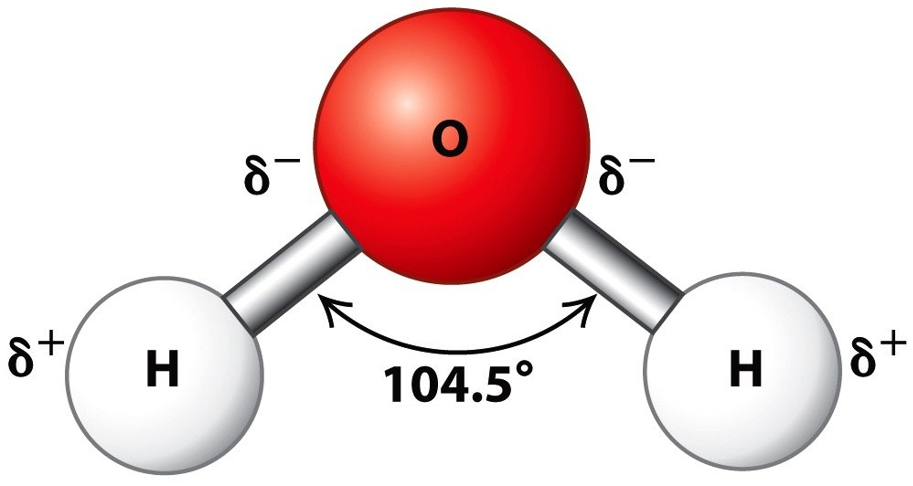
\includegraphics[scale=0.25]{WaterMolecule}
        \caption{Water molecule}
        \label{Water molecule}
\end{center}
\end{figure}
\vspace{0.5cm}

\item Pure water will not conduct electrical current. But when soluble salts such as sodium chloride (NaCl), calcium carbonate (CaCO$_3$) are present in water, water will conduct electricity as these salts ionize - break into its constituent positive and negative charged particles the water, and the charged ions make water to conduct electrical current.
$$NaCl \leftrightarrow Na^+ + Cl^-$$
\item The more ions there are in a solution, the more easily the current flows. The ability to conduct electrical current is called conductivity and can be used to indirectly estimate the amount of total dissolved solids in the water.\\
\item The boiling of water - 100\si{\degree}C or 212\si{\degree}F and its melting/freezing point - 0\si{\degree}C or 32\si{\degree}F is very high  compared to similar molecules and it is the only natural substance found in all three physical states at the temperatures that naturally occur on Earth.
\item Most other substances become more dense as they cool.  However, ice is less dense than water which makes ice float on water.
\item Ice on the water surface insulates the water below preventing it from freezing and allowing for fish and other life form to survive and allows for the movement of animals who live in these cold habitats.
\item As water cools, its density increases upto 4\si{\degree}C after which it gets less dense as it is cooled further.
\item The changing density of water is responsible for turnover of a lake during fall.  When the surface water cools, the cold water becomes more dense than the warm water below so the cold water sinks to the bottom and warm water rises to the top.  When lakes are used as the source water for water treatment plants, turnover can cause abrupt changes in the quality of raw water.
\item It needs a lot of energy to make the water warmer or cooler (high Specific Heat) which allows for keeping the temperature of water bodies such as oceans, rivers, ponds more or less constant despite the heat from the sun.
\item Water molecules stick together well because of its high surface tension - which allows for water to rise up in tubes through capillary action.  This capillary action allows for plants to draw water along with nutrients from the ground.
\end{itemize}


\section{Water use}\index{Water use}
\begin{itemize}
\item Besides it being needed for basic sustenance of all living beings, water is vital element for the world economy and sustenance of the human society in various ways including:
\begin{itemize}
\item As a food source - fishing
\item For commerce - shipping, trade and transportation
\item For recreation - swimming, skiing, surfing etc.
\end{itemize}
\item Breakdown of global freshwater use:\\
70\% is used for agriculture\\
19\% is used by industries, and \\
11\% is for municipal use
\end{itemize}

\section{Water supplies}\index{Water supplies}
\begin{itemize}
\item Civilizations have always formed near water sources - on the banks of rivers. Ancient Egyptians - on the Nile, Mesopotamians in the Fertile Crescent on the Tigris/Euphrates rivers, Ancient Chinese on the Yellow River, and the Ancient India on the Indus.
\item The water on our Earth today is the same water that has been here for nearly 5 billion years.\\
\item Water molecules were formed in interstellar space by chemical reactions between hydrogen molecules and oxygen-bearing molecules such as carbon monoxide and the Earth inherited its water from asteroids and comets crashing into it.
\item The only thing that changes is the form that water takes as it travels through the water cycle.
\item On Earth, water is the only substance that can occur naturally in its three states of matter -  gas, liquid and solids, circulates naturally through its five principal realms:
\begin{itemize}
\item Oceans
\item Atmosphere
\item Lakes and rivers
\item Icecaps and glaciers
\item Underground
\end{itemize}
This is the planetary Water Cycle. \index{Water cycle}
\item Elements of the water cycle include:
\begin{itemize}
\item Transpiration - process by which plants lose water as vapor out of their leaves. 
\item Evaporation - conversion of water in oceans, rives and lakes into vapor by the heat from the sun
\item Evapotranspiration is the combined processes of evaporation and transpiration - the movement of water from oceans or land to the atmosphere.
\item Condensation - cooling of water vapor in the upper layer of earths atmosphere into liquid water in the form of clouds
\item Precipitation - discharge of the water bearing clouds as rain, hail, sleet or snow.
\item Infiltration - movement of water from surface to soil.
\end{itemize} 
\item Life on earth is dependent on the Earth's water cycle \index{Water cycle}
\begin{figure}[]
\begin{center}
\includegraphics[scale=0.8]{Watercycle1}\index{Water cycle}
\caption{Water cycle}
\label{Water cycle}
\textit{(Credit:David Cain/NWS)}
\end{center}
\end{figure}
\item A watershed \index{Watershed} is the area of land, where all of the water that falls in it and drains off of it into to a common outlet which could be a one or combination of water bodies such as a river, lake or underlying groundwater.
\item The natural features including - mountains, trees, shrubs, grasses, and man-made features such as urban area, industries, wastes and water discharges affect the quality of the water in or from the watershed.
\item Watersheds are important sources of drinking water, as well as a habitat for many aquatic species. Healthy watersheds with intact native vegetation and wetlands provide important functions such as water purification, flood control, nutrient recycling, and groundwater recharge.
\item Water covers about 71\% of Earth's surface.  The distribution of Earth's water \index{Distribution of earth's water} is provided in the below table.

% Please add the following required packages to your document preamble:
% \usepackage{multirow}
\begin{table}[ht]
\begin{center}
\begin{tabular}{|l|l|llll}
\hline
\multirow{9}{*}{Fresh water} & \multirow{9}{*}{2.50\%} & \multicolumn{1}{l|}{\multirow{7}{*}{Surface water}} & \multicolumn{1}{l|}{\multirow{7}{*}{1.20\%}} & \multicolumn{1}{l|}{Atmosphere}                & \multicolumn{1}{l|}{3.00\%}  \\ \cline{5-6} 
                             &                         & \multicolumn{1}{l|}{}                               & \multicolumn{1}{l|}{}                        & \multicolumn{1}{l|}{Living things}             & \multicolumn{1}{l|}{0.26\%}  \\ \cline{5-6} 
                             &                         & \multicolumn{1}{l|}{}                               & \multicolumn{1}{l|}{}                        & \multicolumn{1}{l|}{Rivers}                    & \multicolumn{1}{l|}{0.49\%}  \\ \cline{5-6} 
                             &                         & \multicolumn{1}{l|}{}                               & \multicolumn{1}{l|}{}                        & \multicolumn{1}{l|}{Swamps, marshes}           & \multicolumn{1}{l|}{2.60\%}  \\ \cline{5-6} 
                             &                         & \multicolumn{1}{l|}{}                               & \multicolumn{1}{l|}{}                        & \multicolumn{1}{l|}{Soil moisture}             & \multicolumn{1}{l|}{3.80\%}  \\ \cline{5-6} 
                             &                         & \multicolumn{1}{l|}{}                               & \multicolumn{1}{l|}{}                        & \multicolumn{1}{l|}{Lakes}                     & \multicolumn{1}{l|}{20.90\%} \\ \cline{5-6} 
                             &                         & \multicolumn{1}{l|}{}                               & \multicolumn{1}{l|}{}                        & \multicolumn{1}{l|}{Ground ice and permafrost} & \multicolumn{1}{l|}{69.00\%} \\ \cline{3-6} 
                             &                         & \multicolumn{1}{l|}{groundwater}                   & \multicolumn{1}{l|}{30.10\%}                 &                                                &                              \\ \cline{3-4}
                             &                         & \multicolumn{1}{l|}{Glaciers and ice caps}          & \multicolumn{1}{l|}{68.70\%}                 &                                                &                              \\ \cline{1-4}
Other saline   water         & 0.90\%                  &                                                     &                                              &                                                &                              \\ \cline{1-2}
Oceans                       & 96.50\%                 &                                                     &                                              &                                                &                              \\ \cline{1-2}
\end{tabular}
\caption{Distribution of earth's water} \index{Earth's water} \label{Earth's water}
\textit{(From:  Igor Shiklomanov's chapter "Worlds fresh water resources" in Peter H. Gleick (editor), \\1993, Water in Crisis: A guide to the world's Fresh water resources)}
\end{center}
\end{table}

\begin{figure}[]
\begin{center}
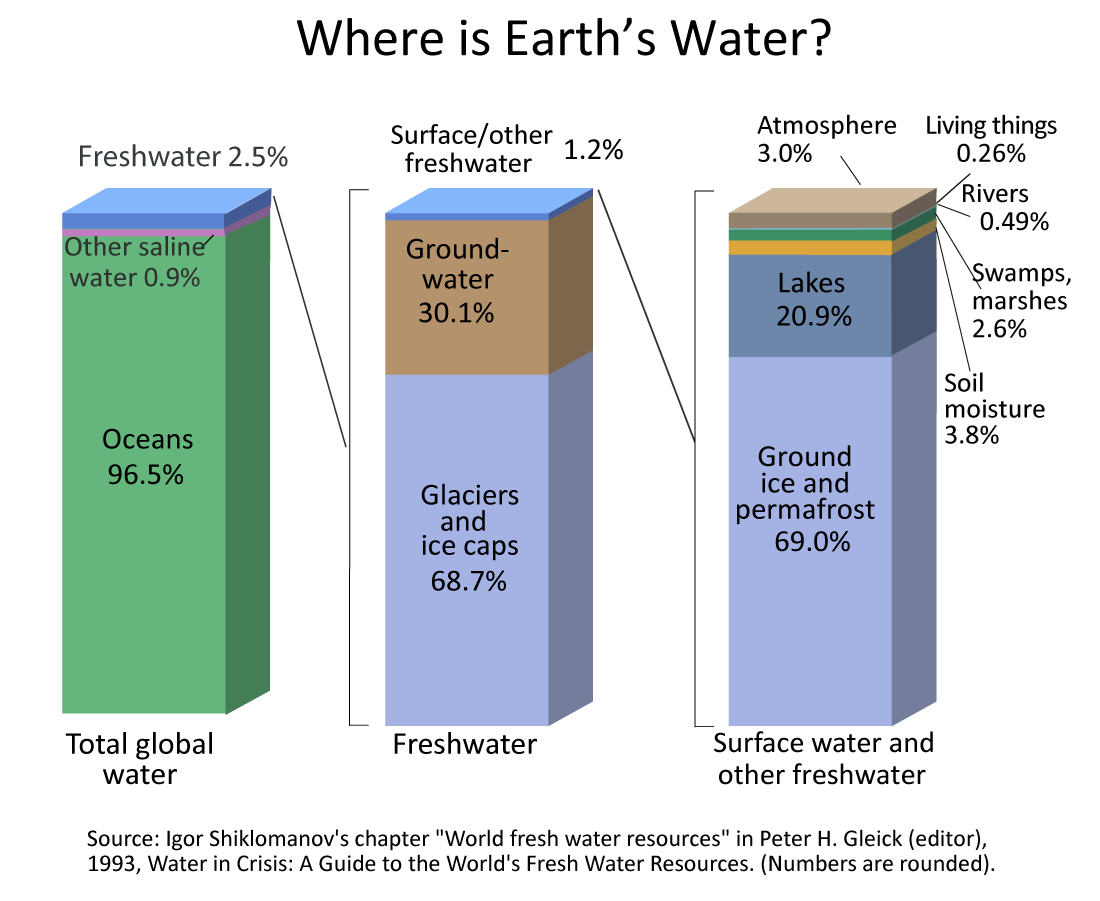
\includegraphics[scale=0.5]{EarthsWater}
\caption{Distribution of earth's water} \index{Distribution of earth's water} \label{Distribution of earth's water}
\textit{(From:  Igor Shiklomanov's chapter "Worlds fresh water resources" in Peter H. Gleick (editor), \\1993, Water in Crisis: A guide to the world's Fresh water resources)}
\end{center}
\end{figure}

\item 97\% of the Earth's water can be found in our ocean and freshwater is only 2.5\% of all the water on earth
\item Most of the fresh water is in form of ice in glaciers, ice caps and permafrost.  
\item A very very small fraction - about 0.006\% of the total water is the freshwater in lakes and rivers.  Most of the remaining freshwater is in groundwater - about 0.75\% of the total water or about 30\% of the total freshwater.
\item Clean water is vital to our health, communities, and economy. 
\item There is no universally accepted definition of “safe drinking water.” Generally speaking, safe drinking water, is defined as the water that does not represent any significant risk to health over a lifetime of consumption.
\item Water scarcity can be caused by a mix of hydrological, infrastructural, political and social issues. 
\item In developing countries, water supply and sanitation related factors cause more than 20 percent of deaths of people under age 14. Nearly
half of all people in developing countries have infections or diseases associated with inadequate water supply and sanitation.
\item Chemical contaminants in drinking water arise including arsenic, fluoride or nitrate, emerging contaminants such as pharmaceuticals, pesticides, per- and polyfluoroalkyl substances (PFASs) and microplastics generate public concern.
\item Microbiologically contaminated drinking water can transmit diseases such as diarrhoea, cholera, dysentery, typhoid and polio and is estimated to cause 485 000 diarrhoeal deaths each year.
\item The amount of water that is available for sustenance including agriculture, sanitation and hygiene is limited in many areas of the world.  Billions of people throughout the world are battling daily against enormous difficulties accessing the most basic services.\\
\item Some 1.1 billion people worldwide lack access to water, and a total of 2.7 billion find water scarce for at least one month of the year.
\item Inadequate sanitation is also a problem for 2.4 billion people.  They are exposed to diseases, such as cholera and typhoid fever, and other water-borne illnesses. Two million people, mostly children, die each year from diarrheal diseases alone.\\
\item Many of the water systems that keep ecosystems thriving and feed a growing human population have become stressed. Rivers, lakes and aquifers are drying up or becoming too polluted to use. More than half the world’s wetlands have disappeared.
\item Climate change is altering patterns of weather and water around the world, causing shortages and droughts in some areas and floods in others, changing large-scale hydrological cycle.\\
\item Historical rates of progress would need to double for the world to achieve universal coverage with basic drinking water services by 2030. 
\item To achieve universal safely managed services, rates would need to quadruple. Climate change, increasing water scarcity, population growth, demographic changes and urbanization already pose challenges for water supply systems. 
\item Re-use of wastewater to recover water, nutrients or energy is becoming an important strategy. 
\item Increasingly countries are using wastewater for irrigation; in developing countries this represents 7\% of irrigated land. While this practice if done inappropriately poses health risks, safe management of wastewater can yield multiple benefits, including increased food production.
\end{itemize}


\section{Water sources}\index{Water sources}
\begin{itemize}
\item Source waters refers to the sources of water - the water bodies or means, which provide water needed for domestic, agricultural and industrial uses.
\begin{figure}[h]
\begin{center}
\includegraphics[scale=0.53]{WaterSources}\\
\captionof{figure}{Water supply sources}%\caption{}
\label{Water supply sources}
\end{center}
\end{figure}
\item Water sources include:
\begin{enumerate}
\item Surface water (for example, a lake, river, or reservoir)
\item Groundwater (for example, an aquifer)
\item Recycled water - also called reused water\\
\end{enumerate}
\end{itemize}
\begin{figure}[h!]
\begin{center}
\includegraphics[scale=0.3]{WaterSupplyIllustration1}\\
\captionof{figure}{Illustration of Southern California water supply systems} \label{Illustration of Southern California water supply systems}
\end{center}
\end{figure}

\begin{figure}[h!]
\begin{center}
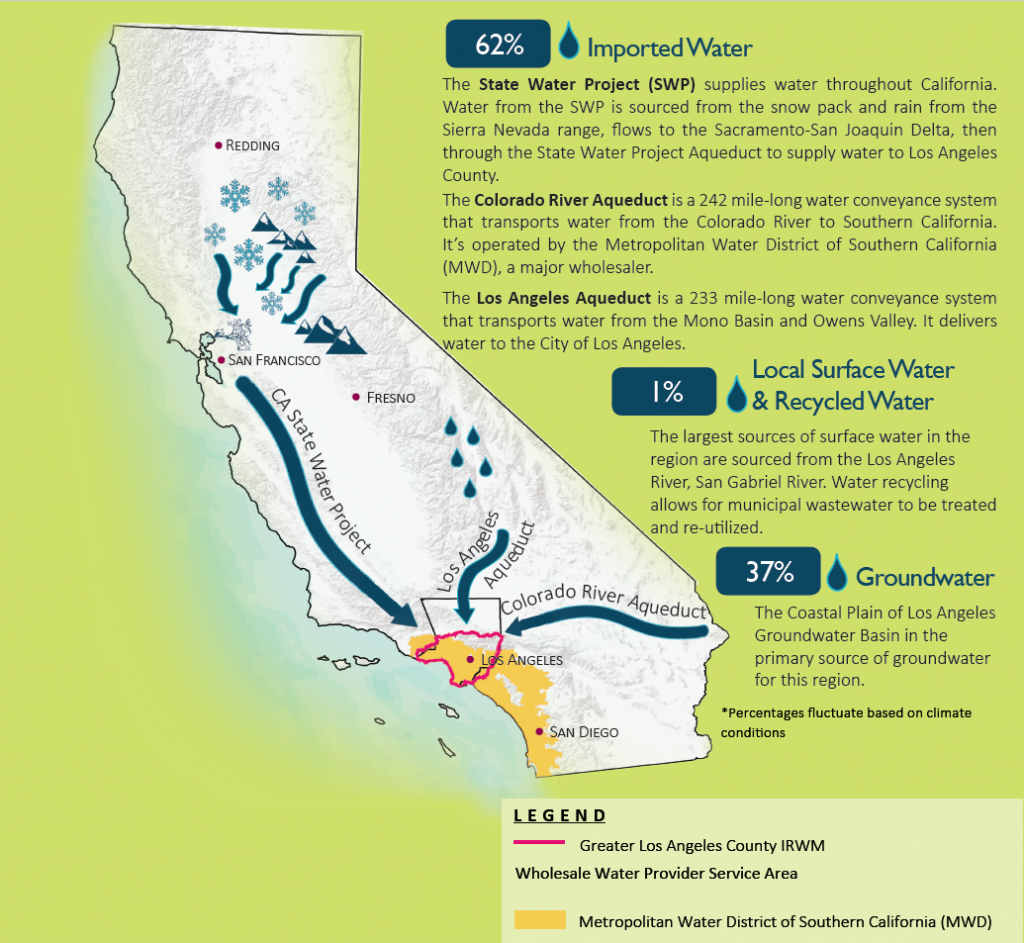
\includegraphics[scale=0.4]{LosAngelesWaterSupply}\\
\captionof{figure}{Los Angeles area source water summary}%\caption{}
\label{Los Angeles area source water summary}
\end{center}
\end{figure}
\subsection{Groundwater}\index{Groundwater}
\begin{itemize}
\item Groundwater is the water found underground in spaces between sand, rock and soil. 
\item Groundwater is stored in aquifers - water-bearing formations underneath the surface that readily transmit water. 
\item \textbf{Aquifers} \index{Aquifer} are underground layers of very porous water-bearing soil or sand with enough groundwater that it can be pumped to the surface and used for drinking water, irrigation, industry, or other uses.
\item Water from precipitation, such as rain or snow, naturally filters through the soil, and is held within the aquifer. 
\item Groundwater can move through the aquifer and resurface through springs and wells.  The rate at which groundwater moves through an aquifer varies depending on the permeability of the layer.
\item Groundwater is extracted from aquifers via well pumping.
\item Groundwater moves from higher elevations to lower elevations and from areas of higher pressure to areas of lower pressure.
\item Groundwater is not stored in huge underground caverns, groundwater fills the pores of the various kinds of rocks that form the earth below us. \textbf{Hydrogeology} is the study of groundwater.
\item The presence of the groundwater depends largely on the geology of a specific area and the variable porosity of the upper portion of the earth’s crust. 

\item Access to groundwater is through:
\begin{enumerate}
\item \textbf{Wells} \index{Wells} - an ordinary well is essentially an a hole in the ground to access the water in the aquifer.
\item \textbf{Artesian Well} - as the groundwater moves in a aquifer, in certain areas of poor permeability, the water is pressurized.  In a well dug in this area, the water level will rise above the top of the aquifer and may even flow onto the land surface - {\textbf{flowing artesian well}}
\item \textbf{Springs} \index{Springs} - which is the flow of groundwater onto the earth's surface through a natural opening.  Springs occur when the contact between an upper aquifer and a lower aquitard intersects the ground surface
\begin{figure}[h]
\begin{tabular}{  m {8 cm}  m {8 cm} } 
\begin{center} \includegraphics[scale=0.6]{GroundWaterSpring} \end{center} & \begin{center}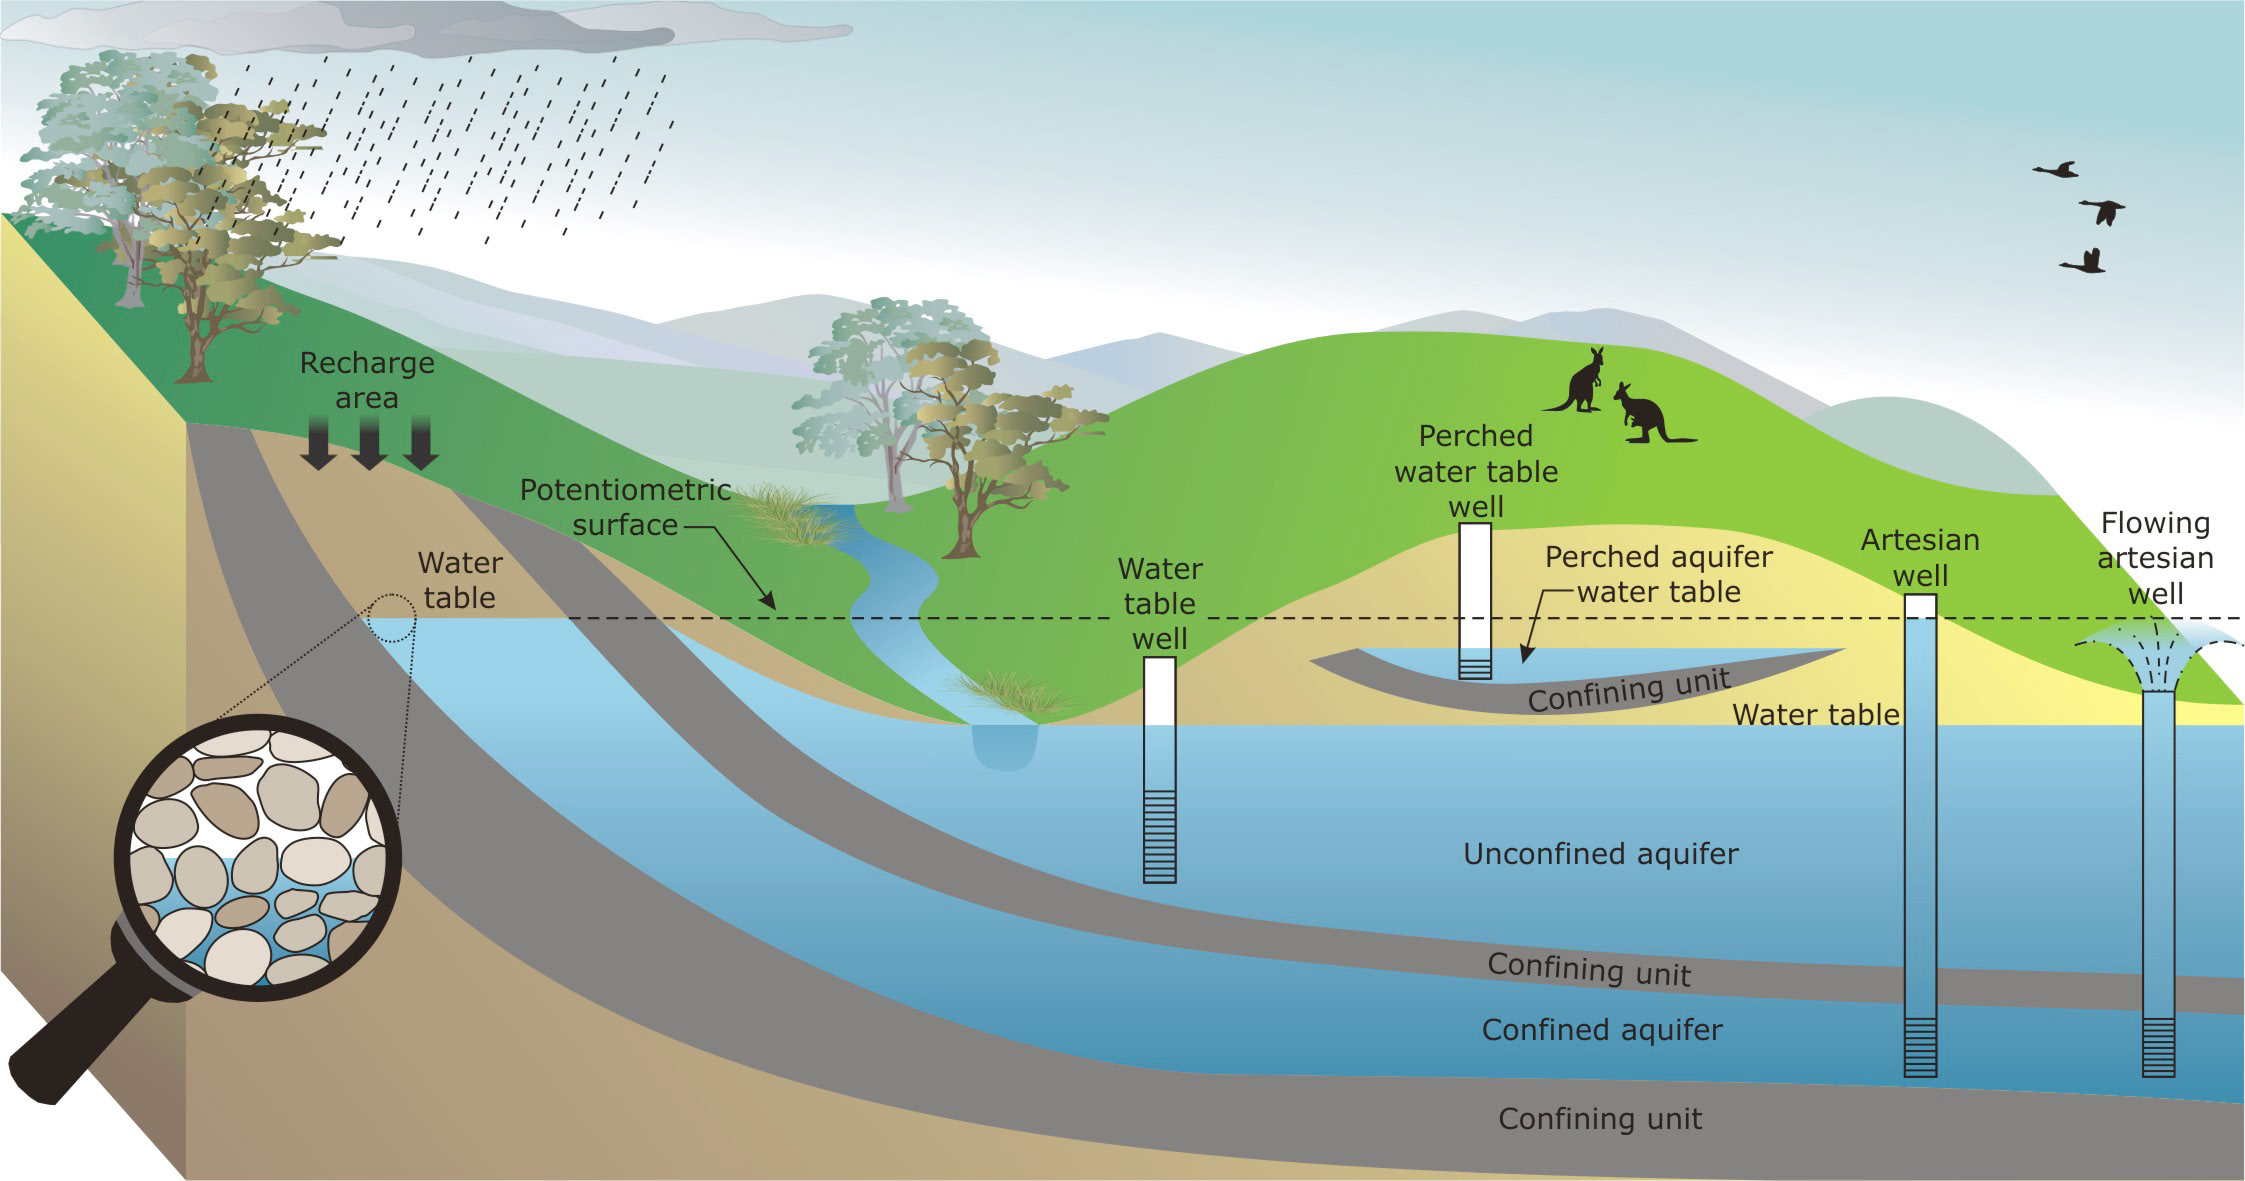
\includegraphics[scale=0.4]{Groundwater1} \end{center}\\
\begin{center} \textbf{Springs} \end{center} & \begin{center}\textbf{Groundwater} \end{center}\\
\end{tabular}\\
\end{figure}
\end{enumerate}
\item There are two general types of aquifers: confined and unconfined. \textbf{Confined Aquifers} \index{Aquifer!Confined and unconfined}have a layer of impenetrable rock or clay above them, while \textbf{Unconfined Aquifers} lie below a permeable layer of soil.
\item The layers of earth which hold the groundwater include a spectrum of layer with porous layer through which the groundwater could through easily in the downward direction, at one end of that spectrum to an \textbf{Aquiclude} which is a geological material through which zero flow occurs.
Then there is the \textbf{Aquitard} \index{Aquifer!Aquiclude, aquitard} in the middle, which is compacted layers of clay, silt or rock that retards the water flow.
\item The replenishment of aquifers by precipitation is called recharging \index{Aquifer!Recharging}. 
\item Aquifers naturally filter groundwater by forcing it to pass through small pores and between sediments, which helps to remove substances from the water. This natural filtration process, however, may not be enough to remove all of the contaminants.
\textbf{Safe yield} \index{Aquifer!Safe yield} is the maximum quantity of water which can be extracted from an aquifer, yet still maintain the supply unimpaired.
\item The \textbf{water table} is the surface of the water level in an unconfined aquifer at which the pressure is atmospheric.  The water table fluctuates due to recharge or outflow from the aquifer,
\item \textbf{Perched water table} is a small water body separated from the main groundwater by a relatively small impermeable stratum.
\item A \textbf{piezometeric surface or a potentiometric surface} \index{Aquifer!Piezometeric surface or potentiometric surface}is an imaginary surface to which the water level would rise if a piezometer - an  instrument used for measuring the pressure of groundwater, is inserted in a well drilled in a confined aquifer.  A piezometeric surface is the water table equivalent of a confined aquifer.
\item Groundwater can become depleted if used at a faster rate than it can be replenished. 
\item Groundwater can become contaminated when an excessive amount of pesticides and herbicides are sprayed on agricultural fields, septic tanks leak, or landfills are improperly lined or managed and toxic materials seep through the soil into the aquifer.
\item Groundwater can be found at nearly every point in the Earth's shallow subsurface to some degree, although aquifers do not necessarily contain fresh water.
\item Most land areas on Earth have some form of aquifer underlying them, sometimes at significant depths. In some cases, these aquifers are rapidly being depleted by the human population.
\item Many parts of the world are heavily dependent on groundwater due to low levels of rainfall.
\item The United States relies on groundwater for 23 percent of its freshwater needs.  In California, that number is significantly higher – groundwater provides nearly 40\% of the water used by California’s farms and cities, and significantly more in dry years.
\end{itemize}

\subsubsection{Water Wells}\index{Water wells}
\textbf{Background}
\begin{itemize}
\item A well is basically a hole in the ground, held open by a pipe (or casing) that extends to an aquifer.
\item A pump draws water from the aquifer for distribution through the plumbing system. 
\item Factors dictating the siting of a well include:
\begin{itemize}
\item Amount of water needed
\item Quality of available water
\item Meet minimum isolation distances required by state rules to ensure safety, and minimize any contamination potential.
\end{itemize}
\item The depth to which wells are constructed is determined by factors including:
\begin{enumerate}
\item depth to groundwater
\item groundwater quality, and 
\item geological conditions at the well site
\end{enumerate}
\end{itemize}
\textbf{Common well terms}\index{Wells!Well terms}:
\begin{itemize}
\item \ul{Static level} \index{Wells!Static level} is the water level in a well when the pump is not operating.
\item \ul{Pumping level} \index{Wells!Pumping level} is the water level in the well when it is producing.
\item Drawdown  \index{Wells!Drawdown} is the difference in elevations between the static level and the pumping level. The amount of water produced is approximately proportional to the drawdown.
\item \ul{Cone of depression}  \index{Wells!Cone of depression} is the depression in the water table formed as the pump draws down the water level.
\item \ul{Zone of influence} \index{Wells!Zone of influence} is the area included in the cone of depression.  Any contamination in this zone will be drawn into the well.
\item \ul{Radius of influence} \index{Wells!Radius of influence} is the farthest distance from the well that the cone
of depression affects the water table.
\item \ul{Specific capacity} \index{Wells!Specific capacity}is the relationship between the yield of a well and the amount of drawdown in the well. It can be expressed as a ratio of the yield, in terms of gallons per minute, to the drawdown in feet. A well producing 100 gpm with a drawdown of 20 feet would have a specific capacity of 5 gpm per foot of drawdown.






%    \begin{minipage}{0.5\textwidth}
%        \centering
%        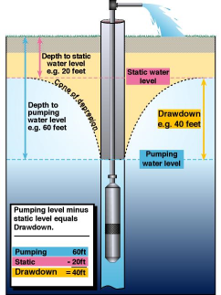
\includegraphics[width=0.75\linewidth, height=0.25\textheight]{WellDrawdownCalc}
%        \caption{Drawdown calculations}
%        \label{fig:prob1_6_1}
%    \end{minipage}








%\begin{figure}[h!]
%\begin{center}
%\includegraphics[scale=0.7]{Welldesign}
%\caption{Well construction}
%\end{center}
%\end{figure}
%\begin{figure}[h!]
%\begin{center}
%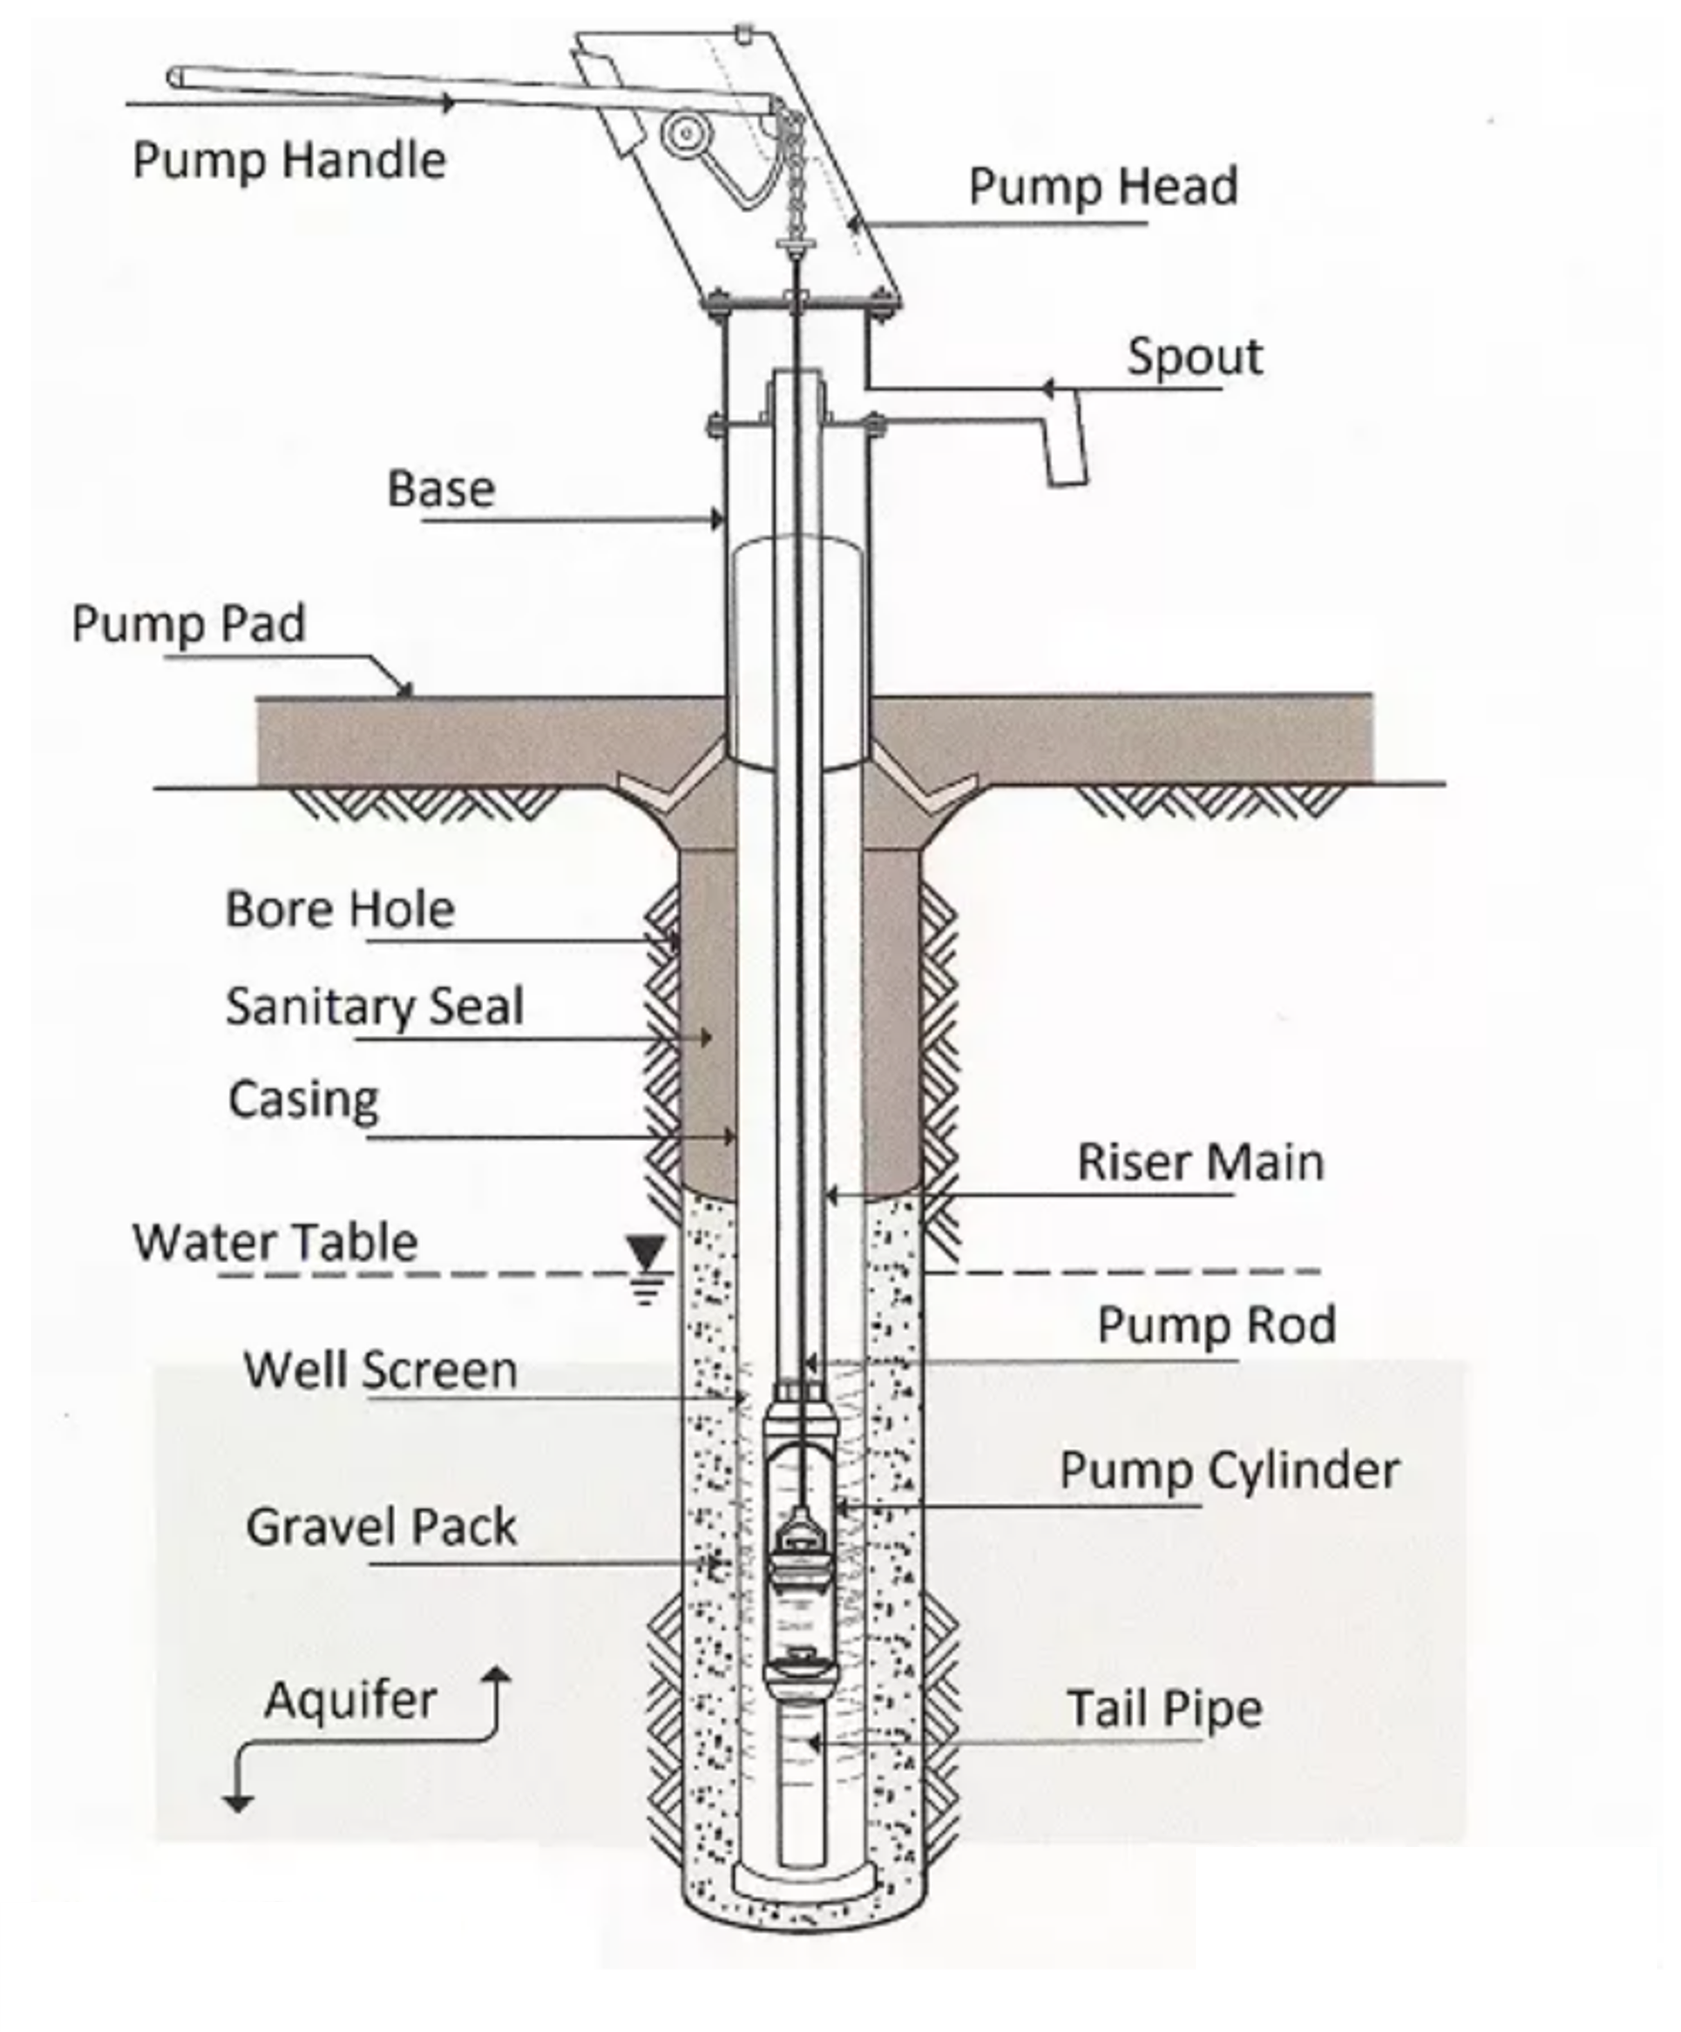
\includegraphics[scale=0.5]{Well}
%\caption{Well calculations}
%\end{center}
%\end{figure}
\item \ul{Recovery time} \index{Wells!Recovery time}is the amount of time required for the aquifer to stabilize at its static water level once pumping has stopped.
\end{itemize}
\begin{figure}[!htb]
    \centering
    \begin{minipage}{0.8\textwidth}
        \centering
        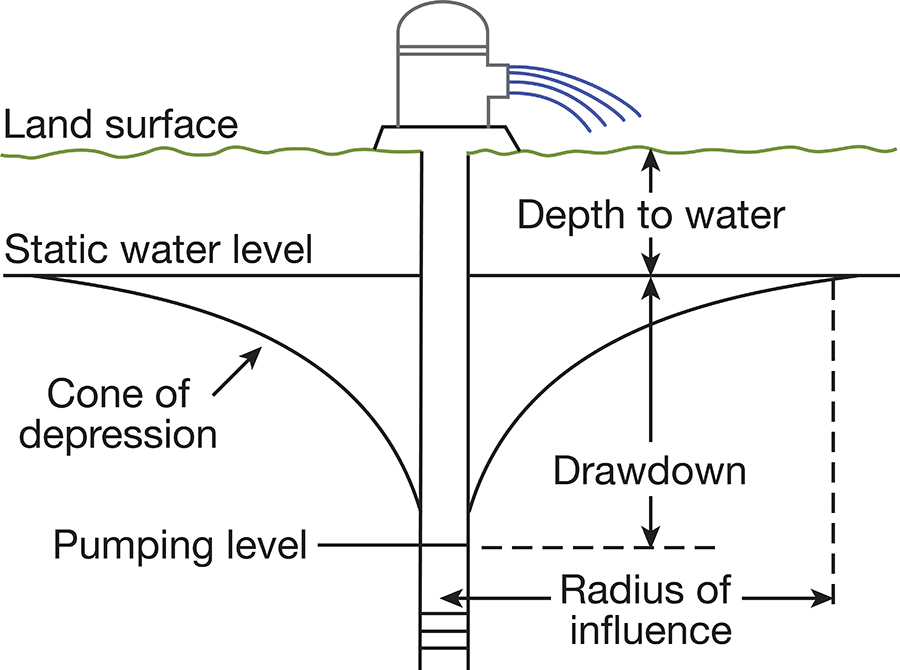
\includegraphics[width=0.6\linewidth, height=0.25\textheight]{WellTermsGraphic2}
        \caption{Well terms}
        \label{Well terms}
    \end{minipage}%
    \end{figure}


\textbf{Well types} \index{Wells!Well types}
\begin{itemize}
\item Wells are classified by method of construction of the well.
\item Well types \index{Wells!Types of wells}include:
\begin{itemize}
\item Dug wells \index{Wells!Types of wells!Dug,driven,drilled wells}:  These wells are typically:
\begin{itemize}
\item large diameter
\item 10-30 ft deep
\item hand-dug to the top layer of the aquifer.  
\item lined with stone or bricks
\end{itemize}
Dug wells levels fluctuate with seasonal variation of water table and has a high risk of contamination from nearby land activities.

\item Driven wells:  These wells are for reaching shallow waters about 30-50 feet deep and are made by driving a small diameter pipe.  Although the well is cased, it has a moderate to high evel of risk of contamination from nearby land activities.

\item Drilled wells:  Drilled well is the most common type of well used by public water systems.  These wells are constructed using a rotary-drilling machine and are hundreds of feet deep.  These wells have a continuous casing, which is commonly six-inches in diameter.  These wells are ideally suited to deep water bearing formations where larger yields are available. This type of well, when properly constructed offers good protection against contamination from the surface.
\end{itemize}

\end{itemize}

\textbf{Well Construction} \index{Wells!Well construction}\\
Elements of well construction include:\\
\begin{itemize}
\item \ul{Borehole} \index{Wells!Wells construction!Borehole} is the narrow shaft drilled to extract water from the aquifer.
item \ul{Well casing} \index{Wells!Well construction!Well casing} is the watertight plastic  or steel tube lining of the borehole.  It is generally 4-6" diameter and it is primarily to protect the borehole from caving in and to prevent surface water from entering the well.  The casing should extend at least 6 to 12 inches above the
well pad, depending on whether the well is located in a well house or out in the open, to prevent standing water from entering the well.
\item \ul{Well screen} \index{Wells!Well construction!Well screen}  is installed on the end of a well casing.  It supports the bore hole, and it reduces the amount of sand that enters the casing and the pump.
\item \ul{Gravel packer} \index{Wells!Well construction!Gravel packer} is a layer of gravel placed around the screen to reduce the amount of fine material from entering the well through the screen.  The gravel packing is usually three times the diameter of the well screen or a minimum of 4" thick.
\item \ul{Grout} \index{Wells!Wells construction!Grout} is cement or bentonite packing around the well casing to protect the well from surface water.  The grout is applied continuously from the surface upto the bottom where the borehole passes into the impermeable layer or upto the gravel packer.
\item \ul{Ground seal} \index{Wells!Well construction!Ground seal}is typically a reinforced concrete slab. This concrete is usually connected to the grout that extends down the well.
\item \ul{Sanitary seal}\index{Wells!Well construction!Sanitary seal} it seals the top of the casing and its primary function is to prevent well contamination.  The type of seal varies depending upon the type of pump being used.  For a well using a submersible pump, the sanitary seal is typically composed of a rubber-like material
placed between two pieces of metal. When bolts are tightened on the sanitary seal, the rubber is compressed and expands to seal against the casing and the pump discharge pipe.
\begin{figure}[h!]
\begin{center}
\includegraphics[scale=0.6]{Welldesign}
\caption{Well construction}
\label{Well construction}
\end{center}
\end{figure}
\end{itemize}
\subsection{Groundwater Under the Direct  Influence  of  Surface  Water}\index{Groundwater under the direct  influence  of  surface  water (GWUDISW)}
\begin{itemize}
\item Groundwater under the direct  influence  of  surface  water (\textbf{GWUDISW}) is the water which may be subject to contamination with pathogenic organisms from surface waters. 
\item GWUDISW is defined as:\\
Any water beneath the surface of the ground with significant occurrence of:\\
\begin{itemize}
\item Insects 
\item Other macroorganisms
\item Algae
\item Large diameter pathogens such as Giardia lamblia
\end{itemize}
\vspace{0.3cm}
or as:\\
\begin{itemize}
\item Any water beneath the surface of the ground with significant and relatively rapid shifts in water characteristics such as:
\begin{itemize}
\item Turbidity
\item Temperature
\item Conductivity, or
\item pH
\end{itemize}
that closely correlates to climatological or surface water conditions.     
\end{itemize}
\end{itemize}

\subsection{Surface water}\index{Surface water}
\begin{itemize}
\item Surface water is water that is open to the atmosphere and results from overland flow. It is also said to be the result of surface runoff. These are two ways of saying the same thing.
\item Examples of surface water include:
\begin{itemize}
\item Streams, Rivers, Lakes
\item Man-made impoundments - Reservoirs
\item Wells drilled next to or in a stream or river
\item Rain catchments
\end{itemize}
\item Surface waters are classified as either:  running waters which include streams, rivers and brooks; and quiescent waters which include lakes and reservoirs.
\
\item  A lake is where surface-water runoff (and maybe some groundwater seepage) have accumulated in a low spot, relative to the surrounding countryside.  Whereas a reservoir is a man-made lake that is created when a dam is built on a river. 
\item The exposure of surface waters to the atmosphere results in exposure to precipitation events, surface water runoff and contamination with micro and macroorganisms resulting from activities in their surrounding areas.

\item Changes in weather cause the natural flow of streams and rivers to vary greatly with time. Periods of excess flows and valley flooding may alternate with low flows or droughts.
\item  The role of water-storage reservoirs, also known as impoundments is to store water during periods of higher flows, thus preventing flood disasters, and then permit gradual release of water during periods of lower flows. 

\item Lakes and reservoirs can be classified into three categories \index{Surface water!Lakes and reservoirs classification} based upon their nutrient content:
\begin{itemize}\index{Eutrophic} \index{Mesotrophic} \index{Oligotrophic}
\item Eutrophic - rich in nutrient
\item Mesotrophic - moderate amount of nutrient 
\item Oligotrophic - little or no nutrient
\end{itemize}
\item In many locations, as the water temperatures decrease with increasing water depth, thermal stratification \index{Lake thermal stratification} - formation of distinct thermal layers, of lakes and reservoirs occur due to temperature related density changes which prevents the vertical mixing of water. 
\begin{enumerate} \index{Epilimnion} \index{Thermocline} \index{Hypolimnion}
\item Epilimnion - Suface layer of warm, light water (mixed by wind)
\item Thermocline or Metalimnion- Middle layer with rapidly changing temperature
\item Hypolimnion - Lowest layer of coldest and densest water. Hypolimnion usually has depletion of dissolved oxygen (DO) leading to fish kills for fish living at that depth.	·
\end{enumerate}

\begin{figure}
\begin{center}
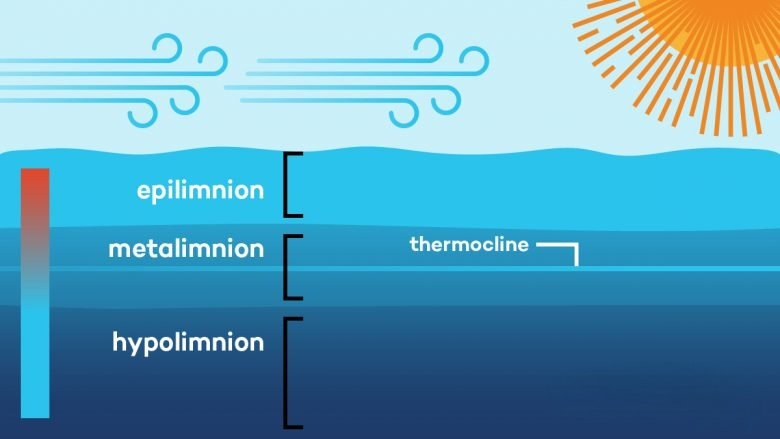
\includegraphics[scale=0.5]{ReservoirStratification}\\
\captionof{figure}{Lake/reservoir stratification}%\caption{}
\label{Lake/reservoir stratification}
\end{center}
\end{figure}
\item Destratification \index{Destratification} - can be natural by change in weather or by means such as aeration or mechanical agitation and mixing.
\item Lake turnover \index{Lake turnover}- During autumn and winter, top layer of water gets colder and denser and
sink to the bottom, water from bottom comes to the top causes the bottom sediments to be stirred	causing high turbidity in the water. It can also cause the heav metals (such as mercury and lead from the bottom of the reservoir become dispersed in the water.

\item Thus, water intakes are located at various levels in the reservoir to get the best possible quality of raw intake water possible at different times of the year.

\end{itemize}

\subsection{Advantages and disadvantages of surface water vs groundwater }\index{Advantages and disadvantages of surface water vs groundwater }
\begin{itemize}
\item Advantages of surface water with respect to groundwater:
\begin{itemize}
\item It is easily located. It takes no sophisticated equipment to find a surface water source.
\item In many parts of the US, considerable data is available on quantity and quality of existing surface water supplies.
\item Surface water is generally softer than groundwater, which makes treatment much simpler.
\end{itemize}
\item Disadvantages of surface water with respect to groundwater:
\begin{itemize}
\item Surface waters can be easily contaminated with microorganisms that cause waterborne diseases and chemicals that enter the stream from surface runoff and upstream discharges.
\item The turbidity of a surface water source often fluctuates with the amount of precipitation. Increases in turbidity increase treatment cost and operator time.
\item The temperature of surface water fluctuates with the ambient temperature. This makes it difficult to produce consistent water quality at a water treatment plant.
\end{itemize}
\item Advantages of groundwater with respect to surface water:\\
\begin{itemize}
\item Groundwater is not as easily contaminated as surface water.
\item The quality of groundwater, while not always as good as would be preferred, is stable throughout the year.
\item Groundwater sources are generally lower in bacteriological count than surface water sources.
\item Groundwater is available in most locations throughout the continental US and Alaska.
\end{itemize}
\item Disadvantages of groundwater with respect to surface water:\\
\begin{itemize}
\item Groundwater usually contains more minerals than surface water, including increased levels of hardness. Because groundwater is in contact longer with minerals, there is more time to bring them into solution.
\item Removal of groundwater normally requires a pump, thus increasing operation cost.
\item Groundwater is more susceptible to long-term contamination from fuel spills.
\item Groundwater supplies often have high levels of iron and manganese, thus increasing treatment cost and/or causing stains on plumbing and the clothing of customers.
\item Wells in the coastal areas are subject to salt water intrusion into the aquifer
and well. This contamination is difficult to predict and costly to treat.
\item Once a groundwater source is contaminated, it is difficult for it to recover. There is no easy way to remove the contaminants. Sources of contamination can be hidden from sight.
\end{itemize}
\end{itemize}
\begin{figure}
\begin{center}
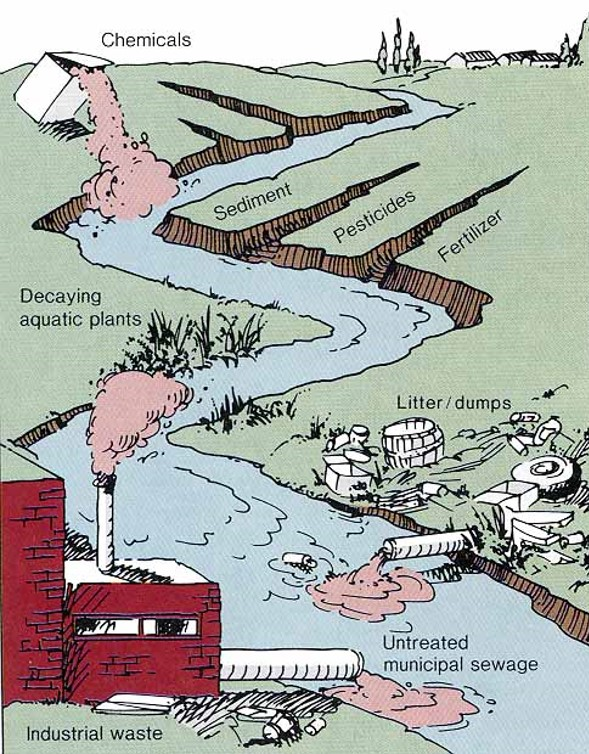
\includegraphics[scale=0.5]{WaterContamination}\\
\captionof{figure}{Sources of water contamination}%\caption{}
\label{Sources of water contamination}
\end{center}
\end{figure}
\subsection{Recycled water}\index{Recycled water}
\begin{itemize}
%\item Within the Water Cycle, there are many subcycles which can be regional or local.
%\item One such cycle is the local cycle which involves water use and reuse.\\
%\begin{figure}
%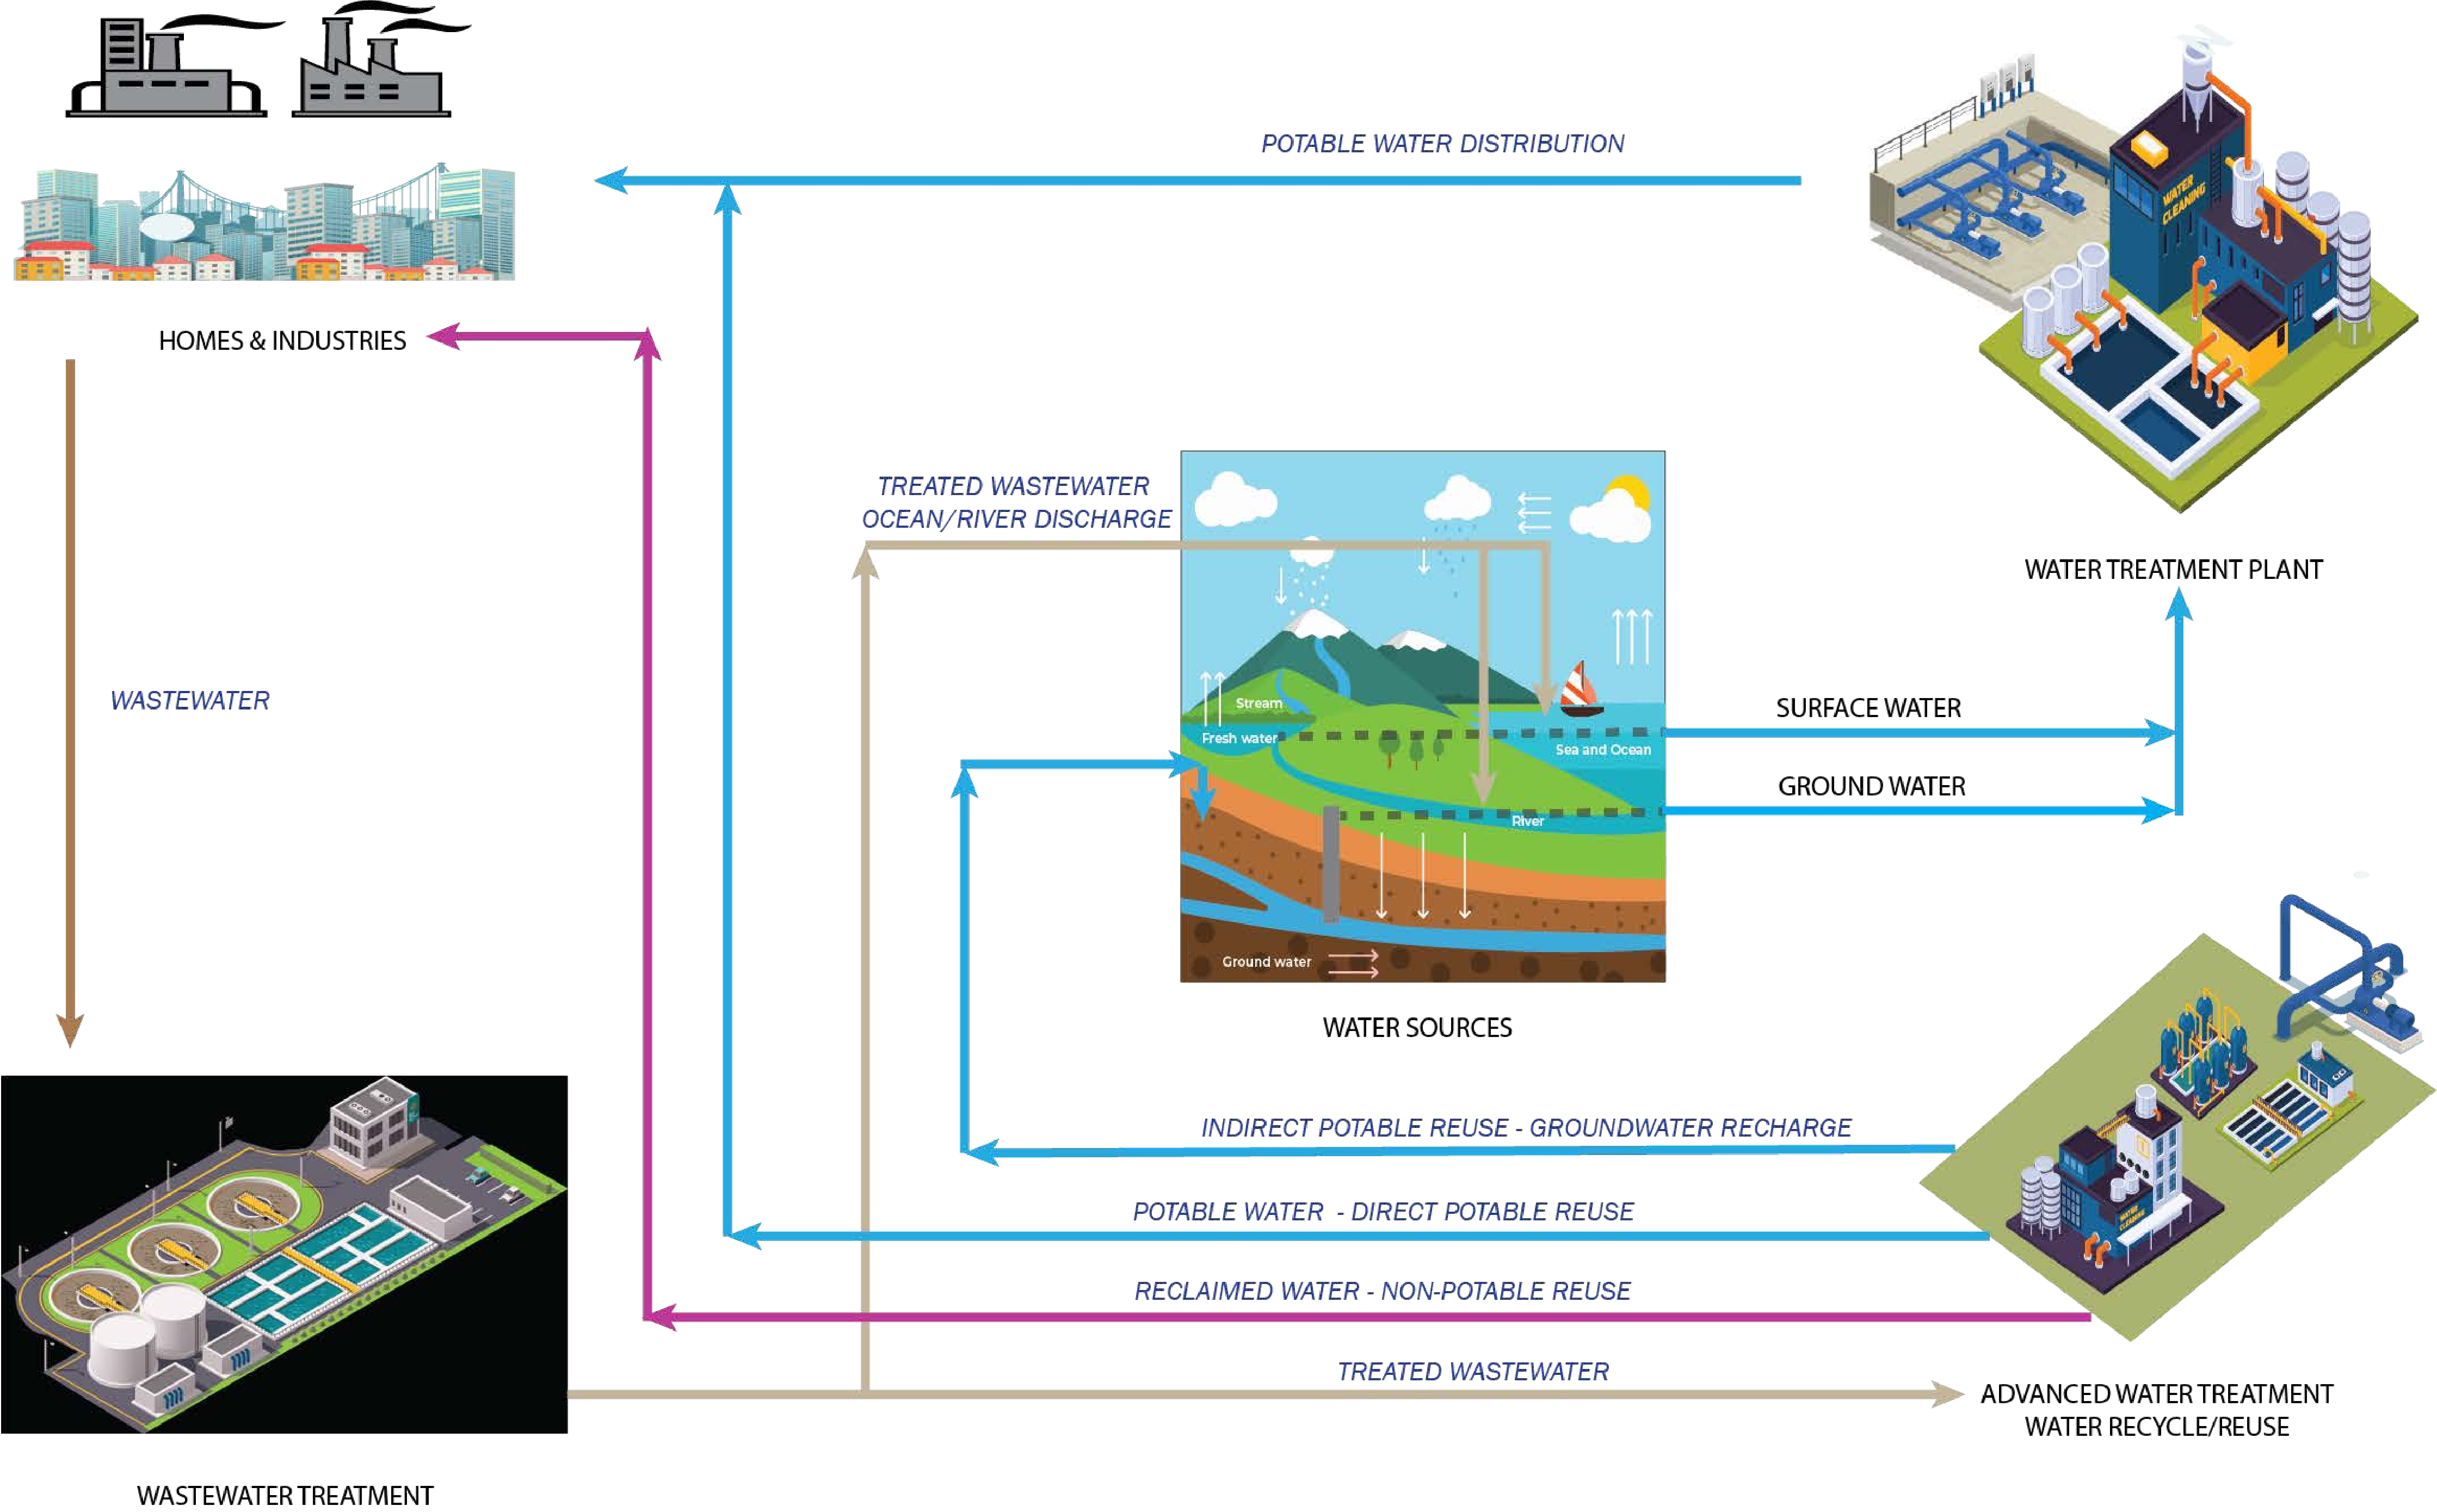
\includegraphics[scale=0.2]{Test4}\\
%\captionof{figure}{Water Use - Reuse Cycle}%\caption{}
%\end{figure}
\item Water reuse (also commonly known as water recycling or water reclamation) reclaims water from a variety of sources then treats and reuses it for beneficial purposes such as agriculture and irrigation, potable water supplies, groundwater replenishment, industrial processes, and environmental restoration.
\item Water reuse can provide alternatives to existing water supplies and be used to enhance water security, sustainability, and resilience.

\item Unplanned or de facto reuse refers to situations in which a source of water is substantially composed of previously-used water. An example of unplanned water reuse occurs when communities draw their water supplies from rivers, such as the Colorado River and the Mississippi River, that receive treated wastewater discharges from communities upstream.
\end{itemize}

\section{Water rights in California}\index{Water rights}
\begin{itemize}
\item If one takes water from a lake, river, stream, or creek, or from underground supplies for a beneficial use, California law requires that person to have a water right. The term “beneficial use” can refer to agricultural, mining, urban, industrial, or environmental uses.
\item In California, water rights law is administered by the State Water Resources Control Board (often called simply the State Water Board). 
\item A water right holder is entitled to a “reasonable” amount of water, which not only considers the purpose for which the water is being used but also the relative consumption of the water with regard to other water users in the system.
\item Two types of water are recognized by law in water with regard to the law: groundwater and surface water.
\item Groundwater is considered a local supply and there is little state regulation of its use,and consequently a state water right permit is not required for use of this water.
\item Primarily, landowners in California are entitled to pump and use a reasonable amount of groundwater from a basin underlying their land to put it to a beneficial, nonwasteful use.
\item The use of surface water is subject to state laws and regulations that control its development and use.
\item Most common surface water rights include:
\begin {enumerate}
\item Riparian rights \index{Water rights!Riparian rights}:\\
\begin{itemize}
\item Riparian rights are rights to the “reasonable and beneficial use of water on land that is adjacent to a watercourse - a lake, river, stream, or creek. 
\item A riparian right allows the landowner to take as much water as can be reasonably and beneficially used on the riparian property. 

\item Riparian owners must share with other riparian owners along the same water body, and they cannot waste water or unreasonably affect public trust resources. 

\end{itemize}

\item{Appropriative Rights} \index{Water rights!Appropriative rights}:\\
\begin{itemize}
\item Appropriative water rights are legal rights to use water from a water source, such as a river or stream, for beneficial purposes.
\item Someone who takes water for use on non-riparian land or who uses water that would not be there under natural conditions on riparian land, appropriates water.
\item These rights are typically granted based on the principle of "first in time, first in right," meaning that the first person or entity to beneficially use the water for a specific purpose has priority over later users. 
\item Appropriative water rights are common in regions where water is scarce and are often subject to regulations and permitting processes to ensure fair and sustainable allocation of water resources.
\item Water right permits and licenses issued by the State Water Board are appropriative water rights.
\item Appropriative water may be stored for later use, or held for diversion and beneficial use.
\end{itemize}

\item Prescriptive Rights \index{Water rights!Prescriptive rights}:\\
\begin{itemize}
\item A prescriptive right is a right that is acquired through adverse possession of someone else’s water right. It is similar to a “squatter’s right” to land.
\item Prescriptive rights originated in the context of conflicts between competing riparian users.
\end{itemize}

\end{enumerate}
\end{itemize}

\chapterimage{QuizCover} % Chapter heading image

\chapter*{Chapter 2 Assessment}
% \textbf{Multiple Choice}
\section*{Chapter 2 Assessment}
\begin{enumerate}[1.]
\item Groundwaters generally have consistent water quality that include\\
a. having a higher total dissolved solids content than surface water\\
b. having a lower mineral content than surface waters\\
c. having lower $\mathrm{pH}$ values than surface waters\\
d. having a higher amount of bacteria than surface waters\\
\item When underground water is under pressure greater than atmospheric pressure and could rise above the its confining space and above the ground level is referred to as a(n)\\
a. aquifer\\
b. anaerobic condition\\
c. artesian effect\\
d. drawdown\\
e. pressure gradient\\
\item The gradual flow or movement of water into and through the pores of the soil is called\\
a. percolation\\
b. run-off\\
c. precipitation\\
d. impermeable flow\\
e. evapotranspiration\\
\item Water that has been used to carry solids away from a home or office into a treatment facility is referred to as\\
a. wastewater or sewage\\
b. potable\\
c. seawater intrusion injection water\\
d. riparian water\\
\item The water right to put it to beneficial use of the surface water adjacent to your land is called water.\\
a. wastewater\\
b. riparian\\
c. filter ripening\\
d. infiltration\\
e. run-off\\
\item The difference between static level and pumping level in a well is called:\\
a. drawdown.\\
b. cone of depression\\
c. zone of saturation\\
d. radius of influence\\
\item Which one of the following best defines the term aquifer?\\
 a. A low lying area where water pools\\
 b. Water-bearing stratum of rock, sand, or gravel\\
 c. Impervious stratum near the ground surface\\
 d. Treated water leaving the water system\\
 \item The height to which water will rise in wells located in an artesian aquifer is called the\\
 a. Pumping water level\\
 b. Water table\\
 c. Piezometric surface\\
 d. Drawdown\\
 e. Radius of influence\\
 \item To prevent the entry of surface contamination into a well is the purpose of\\
 a. The well casing\\
 b. The water table\\
 c. The louvers or slots\\
 d. Well development\\
 e. The annular grout seal\\
 \item An aquifer that is located underneath an aquiclude is called\\
 a. An unconfined aquifer\\
 b. A confined aquifer\\
 c. A water table\\
 d. Unreachable groundwater\\
 e. An Artesian spring\\
 \item The process by which water changes from the gas to the liquid phase is termed\\
 a. Condensation ·\\
 b. Evaporation\\
 c. Percolation\\
 d. Precipitation\\
 e. Runoff\\
 \item The free surface of the water in an unconfined aquifer is known as the\\
 a. Pumping water level\\
 b. Artesian spring\\
 c. Water table\\
 d. Drawdown\\
 e. Percolation\\
 \item The transfer of liquid water from plants and animals on the surface of the earth into water vapor in the atmosphere is called\\
 a. Transpiration\\
 b. Evaporation\\
 c. Condensation\\
 d. Runoff\\
 e. Percolation\\
 \item The elevation of water in the casing of an operating well is called the\\
 a. Piezometric surface\\
 b. Water table\\
 c. Pumping water level\\
 d. Drawdown\\
 e. Radius of influence\\
 \item An aquifer under pressure is often termed\\
 a. Unconfined\\
 b. Pacific\\
 c. Artesian\\
 d. Alluvial\\
 e. Elevated\\
 \item An aquifer is usually composed of\\
a. Sand and gravel\\
b. Clays and silts\\
c. Bedrock\\
d. Large voids in the soil, resembling underground lakes\\
e. None of the above\\
\item Which of the following best defines the term specific capacity?\\
a. Amount of water a given volume of saturated rock or sediment will yield to gravity\\
b. Amount of water a given volume of saturated rock or sediment will yield to pumping\\
c. Rate at which water would flow in an aquifer if the aquifer were an open conduit\\
d. Amount of water a well will produce for each foot of drawdown\\
\item The most common type of well used for public water supply systems is a\\
a. Jetted well\\
b. Driven well\\
c. Drilled well\\
d. Bored well 
\item An aquifer that is underneath a layer of low permeability is known as\\
a. Confined aquifer\\
b. Water Table aquifer\\
c. Unconfined aquifer\\
d. Unreachable groundwater\\
\item What is the middle layer of a stratified lake known as?\\
a. Hypolimnion\\
b. Benthic Zone\\
c. Thermocline\\
d. Epilimnion\\
\item The amount of water that can be pulled from a aquifer without depleting\\
a. Drawdown\\
b. Safe yield\\
c. Overdraft\\
d. Subsidence\\
\end{enumerate}



\part{Chapter 3}
\chapterimage{ChapterImageLaboratory.png} % Chapter heading image

\chapter{Water Quality \& Laboratory Procedures}





% Please add the following required packages to your document preamble:
% \usepackage[normalem]{ulem}
% \useunder{\uline}{\ul}{}
% Please add the following required packages to your document preamble:
% \usepackage[normalem]{ulem}
% \useunder{\uline}{\ul}{}
\begin{table}[H]
\begin{tabular}{| m{1cm} | m{15cm} |}
\hline
\multicolumn{2}{|l|}{\textbf{Expected   Range of Knowledge for Water Properties and Sources}}                                                                          \\ \hline
\multicolumn{2}{|l|}{\textit{Water   Distribution System Operator License Exams}}                                                                                      \\ \hline

D1 & Ability to read   a graduated cylinder                                                            \\ \hline
D1 & Ability to interpret   coliform test results                                                      \\ \hline
D1 & Knowledge of coliform   analysis methods                                                          \\ \hline
D1 & Knowledge of coliform   bacteria types                                                            \\ \hline
D1 & Knowledge of the   definition of pathogenic organisms                                             \\ \hline
D1 & Knowledge of holding   times (e.g. preservatives)                                                 \\ \hline
D1 & Knowledge of water   sampling techniques for bacteriological, organic, and inorganic constituents \\ \hline
D2 & Knowledge of the use   of coliform as a surrogate                                                 \\ \hline
D2 & Ability to   distinguish between presumptive and confirmed results                                \\ \hline
D2 & Knowledge of nitrate   formation in a distribution system                                         \\ \hline
D2 & Knowledge of   potential waterborne diseases                                                      \\ \hline
D2 & Knowledge of the   effects of abnormal pH levels in a distribution system                         \\ \hline
D2 & Knowledge of the   effects of hardness in a distribution system                                   \\ \hline
D2 & Knowledge of the   effects of heterotrophic bacteria in a distribution system                     \\ \hline
D3 & Knowledge of the   galvanic series                                                                \\ \hline
D3 & Knowledge of the   Langelier Index                                                                \\ \hline
D3 & Knowledge of common   inorganic contaminant compounds pH, Conductivity, Hardness, and Turbidity   \\ \hline
D3 & Knowledge of common   organic contaminant compounds                                               \\ \hline
D3 & Knowledge of sources   of inorganic contaminants in a distribution system                         \\ \hline
D3 & Knowledge of sources   of organic contaminants in a distribution system                           \\ \hline
D4 & Ability to interpret a Langelier Index                                                            \\ \hline

\end{tabular}
\end{table}


\newpage



\begin{table}[H]
\begin{tabular}{| m{1cm} |m{15cm} |}
\hline
\multicolumn{2}{|l|}{\textbf{Expected   Range of Knowledge for Water Properties and Sources}}                                                                      \\ \hline
\multicolumn{2}{|l|}{\textit{Water   Treatment Operator License Exams}}                                                                  \\ \hline
T1 & Ability to recognize   abnormal chemical characteristics of water                                 \\ \hline
T1 & Ability to recognize   abnormal odors or colors                                                   \\ \hline
T1 & Knowledge of   chemicals that contribute alkalinity and hardness to water                         \\ \hline
T1 & Knowledge of common   chemical and microbial contaminants in raw water                            \\ \hline
T1 & Knowledge of problems   caused by hard water                                                      \\ \hline
T1 & Knowledge of the   chemical components of groundwater and surface water                           \\ \hline
T1 & Ability to interpret   turbidity information                                                      \\ \hline
T1 & Knowledge of   turbidity causing matter                                                           \\ \hline
T1 & Knowledge of   chemicals that contribute hardness to water                                        \\ \hline
T1 & Ability to recognize   corrosion problems                                                         \\ \hline
T1 & Knowledge of pH   adjustment procedures                                                           \\ \hline
T1 & Knowledge of   corrosion causes                                                                   \\ \hline
T1 & Knowledge of abnormal   taste and odors                                                           \\ \hline
T1 & Knowledge of   chemicals that contribute taste and odor                                           \\ \hline
T1 & Knowledge of taste   and odor treatment processes                                                 \\ \hline
T1 & Ability to recognize   an iron and manganese problem                                              \\ \hline
T1 & Knowledge of health   effects of lead and copper                                                  \\ \hline
T1 & Knowledge of adverse   health effects caused by common contaminants                               \\ \hline
T1 & Ability to collect a   water sample                                                               \\ \hline
T1 & Ability to determine   a proper sampling site                                                     \\ \hline
T1 & Ability to follow   chain of custody                                                              \\ \hline
T1 & Knowledge of   appropriate sample containers and sample sizes                                     \\ \hline
T1 & Knowledge of maximum   holding times                                                              \\ \hline
T1 & Knowledge of proper   sampling and preservation techniques                                        \\ \hline
T1 & Knowledge of well   sampling techniques                                                           \\ \hline
T1 & Knowledge of chemical   hazards                                                                   \\ \hline
T1 & Ability to analyze a   water sample for free and total chlorine                                   \\ \hline
T1 & Ability to read and   interpret a colorimeter                                                     \\ \hline
T1 & Knowledge of approved   analytical procedures for chlorine analysis                               \\ \hline
T1 & Ability to read and   interpret a pH meter                                                        \\ \hline
T1 & Knowledge of acids   and bases                                                                    \\ \hline
T1 & Knowledge of   acceptable water pH range                                                          \\ \hline
T1 & Knowledge of   chemicals that affect the pH of water                                              \\ \hline
T1 & Knowledge of the   effects of pH on water quality                                                 \\ \hline
T1 & Knowledge of the pH   scale                                                                       \\ \hline
T1 & Ability to analyze a   water sample for pH                                                        \\ \hline
T1 & Ability to analyze a   water sample for turbidity                                                 \\ \hline
T1 & Ability to read and   interpret a turbidimeter                                                    \\ \hline
T1 & Knowledge of the   Nephelometric Turbidity Unit (NTU) scale                                       \\ \hline
T1 & Knowledge of   turbidimeter instrumentation                                                       \\ \hline
T1 & Knowledge of   turbidity level requirements                                                       \\ \hline
T1 & Ability to identify   an objectionable taste or odor in water                                     \\ \hline
T1 & Knowledge of   chemicals that contribute taste and odor to water                                  \\ \hline
T1 & Knowledge of the   presence/absence test method                                                   \\ \hline
T1 & Knowledge of approved   analytical procedures for coliform analysis                               \\ \hline
T1 & Knowledge of common   microbial contaminants in raw water                                         \\ \hline
T1 & Ability to interpret   water quality characteristics (hardness, turbidity, pH )                   \\ \hline
\end{tabular}
\end{table}
\newpage



\begin{table}[H]
\begin{tabular}{| m{1cm} |m{15cm} |}
\hline
\multicolumn{2}{|l|}{\textbf{Expected   Range of Knowledge for Water Properties and Sources}}                                                                      \\ \hline
\multicolumn{2}{|l|}{\textit{Water   Treatment System Operator License Exams (Continued)}}                                                                  \\ \hline
T1 & Ability to recognize   abnormal chemical characteristics of water                                 \\ \hline
T2 & Ability to prepare   and calibrate turbidimeter with Primary Standard (Formazin)                  \\ \hline
T2 & Ability to analyze a   water sample for water hardness                                            \\ \hline
T2 & Ability to recognize   abnormal colors in water                                                   \\ \hline
T2 & Knowledge of   Heterotrophic Plate Count (HPC)                                                    \\ \hline
T3 & Knowledge of the   Langelier Index                                                                \\ \hline
T3 & Knowledge of   corrosion control chemical reactions                                               \\ \hline
T3 & Knowledge of iron and   manganese oxidation chemistry                                             \\ \hline
T3 & Knowledge of   chemicals that contribute alkalinity to water                                      \\ \hline
T3 & Ability to use a   titrator                                                                       \\ \hline
T3 & Ability to recognize   a titration endpoint                                                       \\ \hline
T3 & Knowledge of abnormal   alkalinity levels                                                         \\ \hline
T3 & Ability to analyze a   water sample for specific conductance                                      \\ \hline
T3 & Ability to read and   interpret a specific conductance meter                                      \\ \hline
T3 & Knowledge of abnormal   color levels                                                              \\ \hline
T3 & Ability to   distinguish between presumptive and confirmed coliform results                       \\ \hline
T3 & Knowledge of the   multiple tube fermentation method                                              \\ \hline
T3 & Knowledge of the   membrane filtration method                                                     \\ \hline
T4 & Knowledge of the   health effects of fluoride                                                     \\ \hline
T4 & Ability to calculate   a TDS value from a specific conductance reading                            \\ \hline
T4 & Knowledge of EC/TDS   ratio                                                                       \\ \hline
T4 & Ability to calibrate   a specific conductance meter                                               \\ \hline
T4 & Ability to operate an   Ion Specific Electrode (ISE)                                              \\ \hline
T4 & Knowledge of optimal   fluoride level range                                                       \\ \hline
T4 & Knowledge of color   analysis scale                                                               \\ \hline
T4 & Knowledge of true and   apparent color                                                            \\ \hline
T4 & Knowledge of odor   analysis protocol                                                             \\ \hline
\end{tabular}
\end{table}

\newpage
Water occurring in nature will have other elements dissolved or suspended in it. A "contaminant" is a physical, chemical, biological, or radiological substance or matter, in water.  The type and amount of these contaminants will affect the property and safety of that water, if it is to be used as drinking water.  Some drinking water contaminants may be harmful if consumed at certain levels in drinking water while others may be harmless. The presence of contaminants does not necessarily indicate that the water poses a health risk.\\

Contaminants in drinking water can be broadly categorized as:
\begin{itemize}
\item \ul{Chemical contaminants} \index{Chemical contaminants} which may be naturally occurring or man-made elements or compounds. Examples of chemical contaminants include nitrogen, bleach, salts, pesticides, metals, and human or animal drugs.
\item \ul{Biological contaminants} \index{Biological contaminants} which are also refered as micorbes or microbiological contaminants which include bacteria, viruses, protozoa and parasites.
organisms
\item \ul{Radiological contaminants} \index{Radiological contaminants} which are chemical compounds or elements which contain unstable atoms that emit ionizing radiation.  Example of radiological contaminants include, cesium, plutonium and uranium.
\end{itemize}

\section{Organics}\index{Organics}
\begin{itemize}
\item Organics – are carbon based material can originate from lifeforms or can be man-made.
\item Only few carbon compounds such as carbonates, cyanides are not classified as organic.
\item In water they originate from decaying plant and animal life and wastes.
\item Amount present in natural waters is usually low. 
\item Many organic compounds are soluble in water, and surface waters are more prone to contamination by natural organic compounds than are groundwaters.
\item Synthetic organic compounds, such as polychlorinated biphenyls (PCBs), dioxin, and dichlorodiphenyl-trichloroethane (DDT), all of which are toxic, often persist and accumulate because they do not readily break down in natural ecosystems. 
\item Many of the organic compounds found in water are known to cause cancer and birth defects in people. 
\item Organic matter in water is responsible for:
\begin{itemize}
\item Color formation
\item Taste and odor problems
\item Oxygen depletion in streams
\item Interference with water treatment processes, and
\item Formation of halogenated compounds when chlorine is added to disinfect water.
\end{itemize}
\item The quantity of oxygen-consuming organics in water is usually determined by measuring its biochemical oxygen demand (BOD)\index{Organics!Quantification!Biochemical oxygen demand (BOD)}
\item BOD is the amount of dissolved oxygen required by aerobic decomposers to break down the organic materials in a given volume of water over a 5-day incubation period at 20\degree{C} (68\degree{F}).
\end{itemize}

\section{Inorganics} \index{Inorganics}
Inorganic elements do not contain carbon and are not derived from living material. The inorganics include metals, acids, bases, salts, oxides, sulfate, phosphates, etc.
\subsection{Metals}\index{Metals}
\begin{itemize}
\item Iron and Manganese:\\
\begin{itemize}
\item Although iron and manganese are most commonly found metals in groundwaters, surfacewaters may also contain significant amounts at times. 
\item Non-pathogenic bacteria feed on iron and manganese in water to form red-brown (iron) or black-brown (manganese) slime which accumulates on spouts and inside toilet tanks.
\item Iron is a secondary or aesthetic contaminant and dissolved iron gives water a disagreeable metallic taste.
\item An iron concentration of 0.3 mg/l can cause water to turn a reddish brown color and leave reddish brown stains which are very hard to remove.
\end{itemize}
\item Calcium and magnesium: \index{Calcium} \index{Magnesium}\\
\begin{itemize}
\item The metals most often found in the highest concentrations in natural waters are calcium and magnesium. These are usually associated with a carbonate anion and come from the dissolution of limestone rock.
\item Calcium and magnesium are nontoxic and normally absorbed by living organisms more readily than the other metals; therefore, if the water is hard, the toxicity of a given concentration of a toxic metal is reduced. 
\item Conversely, in soft, acidic water, the same concentrations of metals may be more toxic. 
\item In natural water systems, other nontoxic metals are generally found in very small quantities. Most of these will cause taste problems well before they reach toxic levels.
\end{itemize}
\item Heavy metals:\\
\begin{itemize}
\item Even in small quantities, toxic metals including: arsenic, barium, cadmium,chromium, lead, mercury, and silver in drinking water are harmful to humans and other organisms. Arsenic, cadmium, lead and mercury, all cumulative toxins, are particularly hazardous.These particular metals are concentrated by the food chain, thereby posing the greatest danger to organisms near the top of the chain.
\end{itemize}
\end{itemize}
\begin{figure}[]
\begin{center}
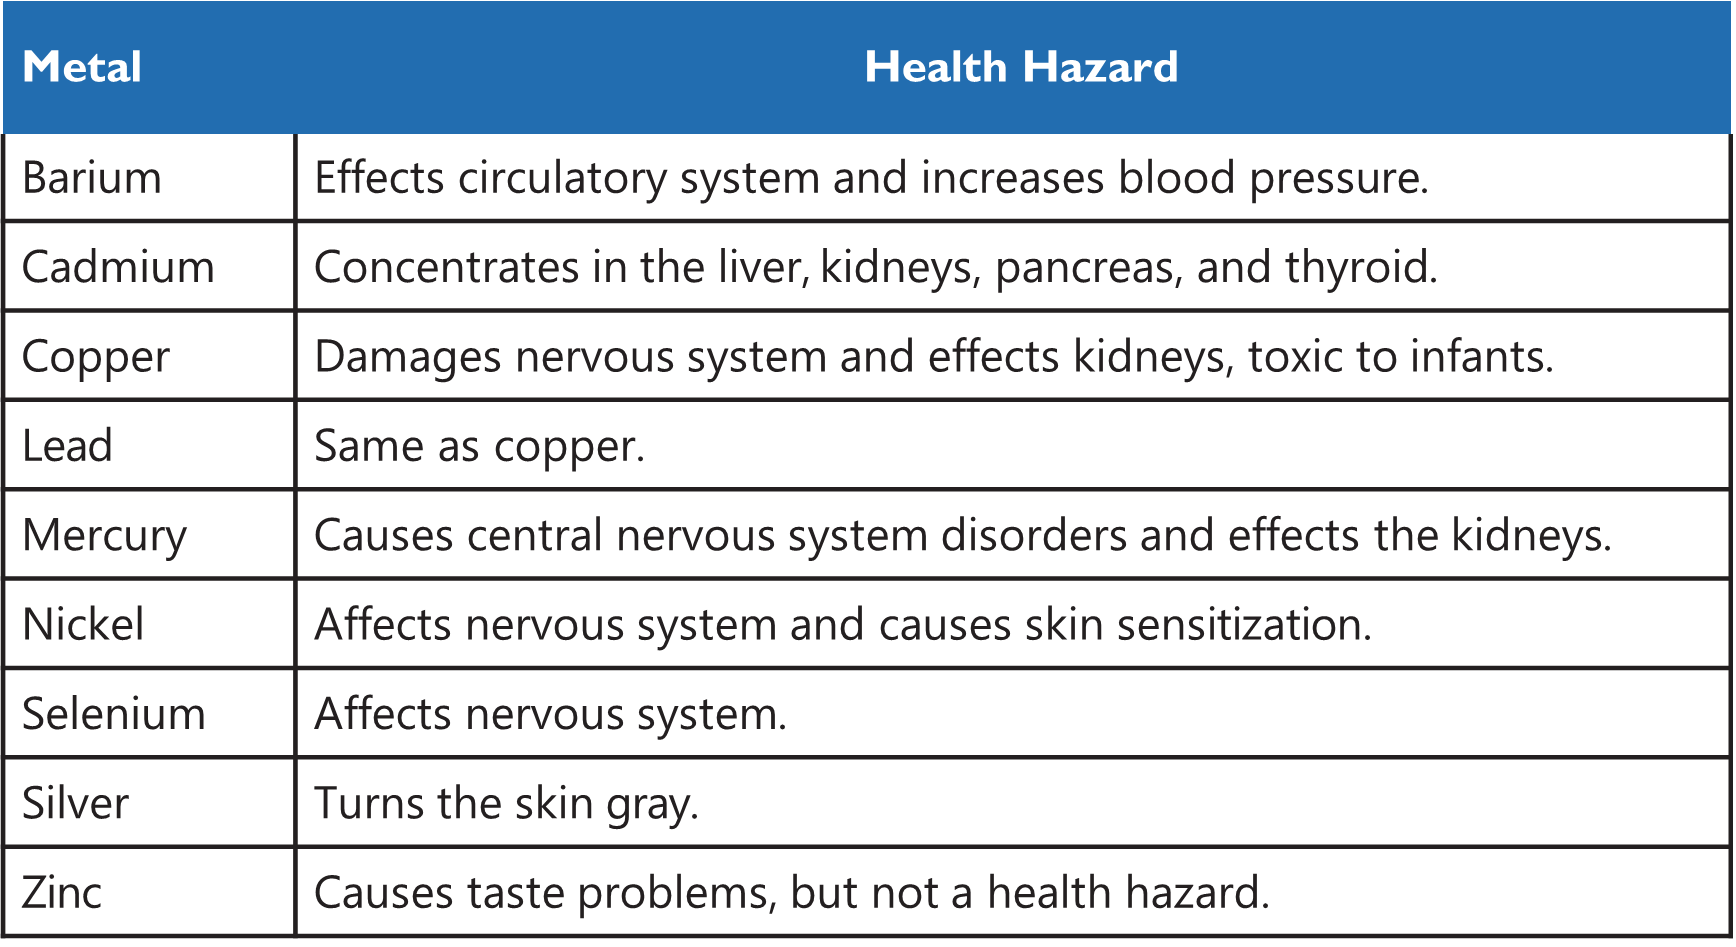
\includegraphics[scale=0.75]{MetalHealthHazard}
\caption{Metals in drinking water - health hazards}\index{Metals!Health hazards}
\end{center}
\end{figure}
\subsection{Salts}\index{Salts}
\begin{itemize}
\item A salt is formed when a metal ion (cation - because it has a positive charge) combines with a nonmetal ion (anion - because it has a negative charge). For instance, when a metal like sodium combines with a non-metal ion like chloride to form sodium chloride, NaCl, or table salt. \index{Anion} \index{Cation}

\item Common metal anions and cations that combine to form salts which are commonly found in drinking water supplies or used in Water treatment are listed in the table below.
\end{itemize}

\begin{table}[h!]    
\begin{center}
     \begin{tabular}{ | m{5cm}  m{5cm} |}
     \hline
           \multicolumn{1}{|c}{} & \multicolumn{1}{c|}{} \\
      \multicolumn{1}{|c}{\textbf{METAL ION (CATION)}} & \multicolumn{1}{c|}{\textbf{NON-METAL ION (ANION)}} \\
            \multicolumn{1}{|c}{} & \multicolumn{1}{c|}{}\\
      Calcium - Ca$^{+2}$ & Carbonate - CO$_3^{\enspace -1}$\\
      Magnesium - Mg$^{+2}$ & Bicarbonate - HCO$_3^{\enspace -1}$\\
      Manganese - Mn$^{+2}$ & Hydroxide - OH$^{-1}$\\
      Iron - Fe$^{+2/+3}$ & Sulfate - SO$_4^{\enspace -2}$\\
      Aluminum - Al$^{+3}$ & Chloride - Cl$^{-1}$\\
      Sodium - Na$^{+1}$ & \\
      Copper - Cu$^{+2/+3}$ & \\
          \hline
                    \end{tabular}
     \caption{Salts constituents}
     \label{Salts constituents}\index{Salts constituents}
     
\end{center}
     \end{table}

\begin{table}[h!]    
\begin{center}
     \begin{tabular}{ | m{5cm}  m{4cm}  m{4cm} |}
     \hline
           \multicolumn{1}{|c}{} & \multicolumn{1}{c}{} & \multicolumn{1}{c|}{}\\
      \multicolumn{1}{|c}{\textbf{CHEMICAL NAME}} & \multicolumn{1}{c}{\textbf{FORMULA}} & \multicolumn{1}{c|}{\textbf{COMMON NAME}}\\
            \multicolumn{1}{|c}{} & \multicolumn{1}{c}{} & \multicolumn{1}{c|}{}\\
      Aluminum sulfate & Al$_2$(SO$_4$)$_3$ & Alum\\
      Calcium oxide & Ca$ $O$ $ $ $ & Quicklime\\
      Calcium hydroxide & Ca$ $(OH$ $)$_2$ & Slaked/hydrated lime\\
      Calcium carbonate & Ca$ $CO$_3$ $ $ & Limestone\\
      Calcium hydroxide & Ca$ $(OH$ $)$_2$ & Slaked/hydrated lime\\
      Magnesium carbonate & Mg$ $(CO$_3$)$_2$ & \\
      Magnesium bicarbonate & Mg$ $(HCO$_3$)$_2$ & \\
      Sodium hydroxide & Na$ $OH$ $ $ $ & Caustic soda\\
      Sodium carbonate & Na$_2$CO$_3$ $ $ & Soda ash\\
      Ferrous sulfate & Fe$ $SO$_4$ $ $ & Copperas \\
      Ferric chloride & Fe$ $Cl$_3$ $ $ & \\
      Ferrous chloride & Fe$ $Cl$_2$ $ $ & \\
      Copper sulfate & Cu$ $SO$_4$ $ $ &\\

          \hline
                    \end{tabular}
     \caption{Salts found in water and/or used in water treatment}
     \label{Salts found in water and/or used in water treatment}\index{Salts found in water and/or used in water treatment}
     
\end{center}
     \end{table}

\subsection{Nutrients}\index{Nutrients}
\begin{itemize}
\item Plant nutrients - nitrogen and phosphorous\index{Nutrients!Nitrogen and phosphorous}, present in water promote growth of plant and algal matter in the receiving waters causing destruction of the normal aquatic life mainly due to oxygen depletion - eutrophication\index{Eutrophication}.
\item Major sources of nitrogen include runoff from animal feedlots, fertilizer runoff from agricultural lands, municipal wastewater discharges, and certain bacteria and blue-green algae than can obtain nitrogen directly from the atmosphere In addition,certain forms of acid rain can also contribute nitrogen to surface waters. Nitrogen in water is commonly found in the form of nitrate (NO$_3^{\enspace-}$) \index{Nitrates}
\item Nitrate in drinking water can lead to serious problems, specifically nitrate poisoning which can lead to death. Bacteria commonly found in the intestinal tract of infants can convert nitrate to highly toxic nitrites (NO$_2^{\enspace-}$). Nitrite can replace oxygen in the bloodstream and result in oxygen starvation, which causes a bluish discoloration of the infant known as infant methemoglobinemia or blue-baby syndrome \index{Infant methemoglobinemia or blue-baby syndrome}.  High nitrate levels may also affect the oxygen-carrying ability of the blood of pregnant women.
\item Nitrifying bacteria present in biological slime in the distribution system convert ammonia and other nitrogen compounds into nitrite (NO$_2$ $^-$) and then nitrate (NO$_3^{\enspace-}$).  This process is called nitrification. \index{Nitrification}
\item Major sources of phosphorous include phosphates in detergents, fertilizers and feedlot runoff, as well as municipal wastewater discharges.
\item Phosphate is added as part of the water treatment for corrosion control and for improving taste and odor by sequestering iron and magnesium.

\end{itemize}

\section{Trace constituents} \index{Trace constituents}
\begin{itemize}
\item Trace Constituents are chemicals found in extremely low concentrations.
\item Trace constituents include:
\begin{itemize}
\item B - Boron
\item Miscellaneous metals
\item Hormones
\item EDCs - Endocrine-disrupting compounds are synthetic and natural compounds that mimic, block, stimulate, or inhibit natural hormones in the endocrine systems of animals, including humans. The origins include pesticides, pharmaceutically active chemicals (PhACs), personal care products (PCPs), herbicides, industrial chemicals, and disinfection byproducts (DBPs).
\item PCPs - Personal Care Products are products such as shampoo, hair conditioner, deodorants, and body lotion.
\item Pharmaceuticals - aspirin, ibuprofen, caffeine, etc.
\item CECs - Constituents of Emerging Concern is a general term applied to constituents that have relatively recently become known as a potential concern and likely have little to no information available to fully comprehend and establish safe and realistic standards, such as PFAS/PFOA \index{PFAS/PFOA}.
\index{Trace constituents!Boron, hormones, EDCs, PCPs, CECs, PFAS/PFOA}
\end{itemize}
\end{itemize}

\section{Radionuclides}\index{Radionuclides}
\begin{itemize}
\item Radioactive materials, also called radionuclides, are both naturally occurring and human-made.

\item Radionuclides such as radium, radon and uranium can get into groundwater and surface waters from natural sources and also potentially from human sources such as active nuclear power plants or other facilities that make or use radioactive substances.

\item When radionuclides break down (decay), they emit radioactive particles such as alpha-particles, beta-particles and gamma-rays radiation which could present a risk to human health.

\item Most water systems have no detectable radionuclide activities, some areas of the United
States have significantly higher levels than the national averages.

\item People who are exposed to relatively high levels of radionuclides in drinking water for long periods may develop serious health problems, such as cancer, anemia, osteoporosis, cataracts, bone growths, kidney disease, liver disease and impaired immune systems.

\item The health risks associated with radionuclides are normally small compared with the risks from microorganisms and chemicals that may be present in drinking-water. 

\item The amount of radionuclides in drinking water is quantified and regulated under the EPA's Radionuclide Rule, by standards based upon both, the radioactivity levels as measured by the radiation of alpha and beta particles and the amount of commonly found radioactive elements - radium and uranium, quantified in terms of their radioactivity.
\item For drinking water, radiation/radioactivity levels is measured as pCi/L (picocuries per liter)\index{Radionuclides!Measurement!picocuries per liter (pCi/L)}
\end{itemize}



\section{Microbial contaminants}\index{Microbial contaminants}
\begin{itemize}
\item Many types of \textbf{pathogenic} - disease-causing germs can be found in contaminated drinking water, including bacteria, viruses and parasites.

\item Common virus in drinking water \index{Pathogens!Viruses} source and their associated diseases include:
\begin{itemize}
\item Adenoviruses - tonsillitis, conjunctivitis, the common cold and other illnesses. 
\item Reoviruses - colds, flu, diarrhea, chicken pox, measles and mumps.
\item polioviruses - polio
\item hepatitis A virus
\end{itemize}

\item Some of the water borne pathogenic bacteria \index{Pathogens!Bacteria} and their associated disease include:
\begin{itemize}
\item Salmonella typhi - Typhoid fever
\item Vibrio cholerae - cholera
\item Yersinia enterocolitica - gastroenteritis
\end{itemize}

\item Common intestinal parasites and their associated disease include \index{Pathogens!Parasites}:
\begin{itemize}
\item Entamoeba histolytica - Amoebic Dysentery.
\item Giardial lamblia (Giardiasis) \index{Pathogens!Parasites!Giardia}.
\item Ascaris lumbricoides (Giant Roundworm).
\item Cryptosporidium (Cryptosporidiosis) \index{Pathogens!Parasites!Cryptosporidium}.
\end{itemize}


\end{itemize}
 



\section{Physicochemical tests} \index{Physicochemical tests}

\begin{itemize}
\item The aesthetic quality \index{Aesthetic quality} aspects of drinking water include: taste, odor, color, turbidity, hardness, and temperature.
\item The aesthetics are generally not health-related. However, consumers can easily detect them, so they can have significant effects on perceptions of water quality and acceptability.
\item These attributes are the source of most complaints to water suppliers and frequently lead consumers to choose home treatment or bottled water.
\end{itemize}
\subsection{Turbidity}\index{Turbidity}
\begin{itemize}
\item Measures cloudiness of water due to suspended particles.
\item Higher turbidity levels are often associated with higher levels of disease-causing microorganisms.
\item Turbidity affects both the acceptability of water to consumers
\item Harmful pollutants such as heavy metals and pesticides are easily absorbed by suspended solids
\item Turbidity affects disinfection as suspended particles in water act as a protective shield for micro-organisms and provide an excellent substrate for bacteria growth.  Higher disinfection doses or contact times are required to ensure adequate treatment.
\item Suspended solids represent a risk for the main water distribution systems, pumps and other equipment where tend to deposit and block pipes and nozzles.
\item Turbidity is an optical measurement of water's ability to scatter and absorb light rather than transmit it in straight lines.  It is commonly measured in the unit of Nephelometric Turbidity Units (\textbf{NTU}). \index{Nephelometric Turbidity Units (NTU)}
\item "Crystal-clear” water has a turbidity of <1 NTU; at 4 NTU and above, water becomes visibly cloudy at 25 NTU it is murky.
\item An average person is able to see turbidity with the naked eye at NTU level of 5 and above.
\item Sources of turbidity:
\begin{enumerate}
\item In source water, turbidity can be attributed to:
\begin{itemize}
\item Inorganic particles released by weathering of rocks, soils and clays
\item Human, livestock and industrial wastes
\item Biological growth (e.g. algae, zooplankton and cyanobacteria) in source waters
\item Natural organic matter including decomposing plant material
\end{itemize}
\item Introduction of turbidity during treatment can be due to:
\begin{itemize}
\item Poor control of treatment chemical dosing (e.g. coagulants, settling aids and pH adjustment chemicals)
\item Precipitates from insoluble components of treatment chemicals, or formed during processes such as pH correction
\item Oxidation products of natural chemicals such as arsenic, iron and manganese
\end{itemize}
\item Turbidity can also be introduced in the distribution system by: \index{Turbidity}
\begin{itemize} 
\item Intrusion of soils and sewage through mains breaks
\item External contamination from backflow or cross connections
\item Resuspension of accumulated silts and sediments, or detachment of corrosion chemicals and scales and detachment of biofilms
\end{itemize}
\end{enumerate}
\item Formazin \index{Formazin} - a chemical, is used for preparing solutions of known turbidities.
\end{itemize}

\subsection{Color}\index{Color}
\begin{itemize}
\item Color may affect the turbidity value but is distinct from turbidity as color is due to organic material that has dissolved into solution, while turbidity consists of tiny particles suspended in the water column.
\end{itemize}

\subsection{Taste and odor}\index{Taste and odor}
\begin{itemize}
\item Odor and taste are useful indicators of water quality even though odor and taste-free water is not necessarily safe to drink nor water with some odors or taste is necessarily harmful.
\item Taste and odors are often grouped with odor because of their common origin factors. 
\item The cause of taste and odor issues can be from water fixtures, plumbing materials, water heaters, water treatment, pressure tanks and/or the source (the well).
\item Taste and odors are generally attributed to the presence of organic and some inorganic chemicals which come from the decaying organic matter, runoffs, industrial wastes, and municipal sewage discharges. 
\item Geosmin and methyl-isoborneol (MIB) are often the cause of earthy-musty odors occurring in fall due to the turnover of lakes and reservoirs.  They are produced by bacteria, particularly actinomycetes and cause odor issues at a very low concentrations.
\item In the groundwater, the tastes and odors can be due to iron, manganese, and hydrogen sulfide (H$_2$S).
\item Often, identifying the exact origin of taste and odor is usually very expensive and often impossible, and removal of the causative substance is even harder.
\item Current methods of measuring taste and odor are still fairly subjective.  Standards related to odor and taste: Chloride, Copper, Foaming Agents, Iron, Manganese pH, Sulfate, Threshold Odor Number (\textbf{TON})\index{Threshold odor number (TON)} which is the greatest dilution of a sample with odor-free water that still yields a just-detectable odor.
\end{itemize}

\subsection{Temperature}\index{Temperature}
\begin{itemize}
\item Temperature affects the solubility of oxygen in water, the rate of bacterial activity, and the rate at which gases are transferred to and from the water.
\item Cool water is generally more palatable than warm water, and temperature will have an impact on the acceptability of a number of other inorganic constituents and chemical contaminants that may affect taste. 
\item High water temperature enhances the growth of microorganisms and may increase problems related to taste, odor, color and corrosion.
\item Water temperature determines, in part, how efficiently certain water treatment processes operate. For example, temperature has an effect on the rate at which chemicals dissolve and react. When water is cold, more chemicals are required for efficient coagulation and flocculation to take place. When water temperature is high, the result may be a higher chlorine demand because of the increased reactivity, as well as an increased level of algae and other organic matter in raw water.
\item Heat is added to surface and groundwater from natural and man-made sources.  Surface waters in particular  are potentially subject to great temperature variations. 
\item Other sources of increased temperatures in running water result from forest clearing and return of irrigation flows to a body of running water.
\end{itemize}

\subsection{Total dissolved solids}\index{Total dissolved solids}
\begin{itemize}
\item Total dissolved solids (\textbf{TDS}) is a part of total solids (\textbf{TS}) in water and are the material remaining in water after filtration.
\item Components of water TDS include:
\begin{itemize}
\item Minerals from rocks and soil as water passes over and through them.
\item Pesticides and herbicides from agricultural runoff
\item Lead and copper from plumbing pipes
\item Chemicals added during water treatment
\item Human and animal wastes
\item Biological decay products
\end{itemize}
\item Water has an equilibrium state with respect to dissolved portion; thus, if water is under saturated, it will aggressively dissolve materials it comes into contact with. Because of this problem, certain soluble substances, typically calcium and magnesium based substances are added post water treatment to minimize its corrosivity effects in the distribution system.
\item Dissolved solids can be removed from water by distillation, electro-dialysis, reverse osmosis, or ion exchange.
\item TDS is measured in mg/L or ppm.  
\item As water will conduct electricity due to the presence of dissolved inorganic ions, higher the concentration of these ions, the higher is the conductivity. Thus, specific conductance \index{Specific conductance} - conductivity measurement, provides a good estimate of the water's TDS.
\item The terms “specific conductance,” “specific electrical conductance,” and
“electrical conductivity” are used interchangeably and its unit of measurement is in Siemens per centimeter (S/cm) or mhos per centimeter (mhos/cm) \index{mhos per centimeter (mhos/cm)} \index{Siemens per centimeter (S/cm)}.
\item The TDS concentration is considered a Secondary Drinking Water Standard, which means that it is not a health hazard.
\item EPA has established a Secondary Drinking Water Standard of a maximum concentration of 500 mg/l of TDS \index{Total dissolved solids!Secondary standard}in drinking water and  recommends treatment when TDS concentrations exceed 500 mg/L, or 500 parts per million (ppm). 
\end{itemize} 

\subsection{pH}\index{pH}	
			pH is a measure of the hydrogen ion (H$^+$) content or the acidity or basicity of a solution.  pH impacts the chemical and microbiological elements of water treatment processes and thus pH measurement and control is critical.
			\begin{itemize}
				\item Pure water dissociates into equal concentration of hydrogen ions and hydroxide ions:\\ 
				      $H_2O \rightarrow H^+ + OH^-$.
				\item The H$^+$ are responsible for acidic properties and the OH$^-$ ions for the basic properties.  
				\item pH is the inverse of H$^+$ concentration; pH increases when the concentration of H$^+$ decreases relative to the concentration of OH-. 
				\item pH scale ranges from 0 – 14. When the concentration of both H$^+$ and OH$^-$ are equal, as in pure water, it is considered neutral and its pH is 7.0.  \item If the pH of a sample solution is below 7.0, the sample is termed acidic and is alkaline or basic if its pH is above 7.0. 
				\item Each change of 1 pH unit represents a 10 fold change in concentration.  For example, a sample with a pH of 2.0 is 1000 times more acidic than a sample with a pH of 5.0.
				
				\item The affects of drinking water pH include:
				\begin{itemize}
				\item Taste and odor impacts.
				\item Solubility and biological availability of chemical constituents such as nutrients - phosphorus, nitrogen, and carbon.
				\item Solubility and toxicity of heavy metals.  Metals tend to be more toxic at lower pH because they are more soluble.
				\end{itemize} 
				\item pH is measured by an electrode that is sensitive only to H$^+$ or using a pH strip which is essentially an adsorbent paper which is pre-impregnated with chemicals which change color under different H$^+$ concentrations.
						
\item \index{pH!pH measurement}It is important to measure pH at the same time as chlorine residual since the efficacy of disinfection with chlorine is highly pH-dependent; where the pH exceeds 8.0, disinfection is less effective. To check that the pH is in the optimal range for disinfection with chlorine (less than 8.0), simple tests may be conducted in the field using comparators such as that used for chlorine residual. With some chlorine comparators, it is possible to measure pH and chlorine residual simultaneously.

\item Alternatively, portable pH electrodes and meters are available. If these are used in the laboratory, they must be calibrated against fresh pH standards at least daily; for field use, they should be calibrated immediately before each test. Results may be inaccurate if the water has a low buffering capacity.
\end{itemize}

\subsection{Alkalinity}\index{Alkalinity}
\begin{itemize}
\item Alkalinity is a measure of the ability of water to neutralize acid, or an expression of its buffering capacity.
\item Constituents of alkalinity are: Bicarbonate – HCO$_3$, Carbonate - CO$_3$ , Hydroxide - OH$^-$
\item Measured in equivalent of mg/L CaCO$_3$
\item Alkalinity levels can be classified as:
\begin{itemize}
\item Low Alkalinity - < 20 mg CaCO$_3$/L
\item Moderate Alkalinity - 20 to 160 mg CaCO$_3$/L
\item High Alkalinity - > 160 mg CaCO$_3$/L
\end{itemize}
\item High alkalinity indicates the scaling (deposit forming) potential and salty taste
\item Low alkalinity implies undersaturation of water (absence of dissolved content) and thus would exhibit higher corrosion potential - tendency to dissolve metals.
\item Alkalinity originates naturally as water moves through rocks dissolving minerals.
\item Alkalinity is important for fish and aquatic life because it protects or buffers against rapid pH changes. In addition, alkalinity levels affect the efficiency of certain water treatment processes, especially the coagulation process.
\end{itemize}


\subsection{Hardness}\index{Hardness}
\begin{itemize}
\item Hardness is due to the presence of multivalent metal ions, which come from minerals dissolved in water.  The dissolution of these minerals is aided by the carbonic acid formed by the dissolution of naturally occurring carbon dioxide in water. 
\item Domestic use of hard water is marked by lack of foam formation with soap solutions due to the formation of a white precipitate (soap scum) instead of producing lather and formation of noticeable limescale in kettles and water heaters.
\item Calcium (Ca) and Magnesium (Mg) \index{Calcium} \index{Magnesium} are the two metals that dissolve the most easily in water. They are considered to be the main cause of hardness.
\item Hardness causing compounds are broken into two groups:\\
\begin{itemize}
\item \ul{Carbonate hardness or temporary hardness} \index{Carbonate hardness or temporary hardness}which is the hardness that can be removed by boiling water.
\begin{itemize}
\item Carbonate hardness is formed when calcium or magnesium combines with a form of alkalinity (carbonate, bicarbonates, or hydroxides.) 
\end{itemize}
\item \ul{Non-carbonate hardness} \index{Hardness!Carbonate hardness} cannot be removed by boiling water.
\begin{itemize}
\item Non-carbonate hardness \index{Hardness!Non-carbonate hardness}is formed when calcium and magnesium combine with anything other than alkalinity. Chlorides and sulfates are the two most common forms of non-carbonate hardness.
\end{itemize}
\end{itemize}
\item Hard water when used in industrial applications forms deposits - scale composed mainly of calcium carbonate (CaCO$_3$), magnesium hydroxide (Mg(OH)$_2$), and calcium sulfate (CaSO$_4$)on the inside surfaces of pipes and heat exchangers. The scale formed restricts the flow of water, heat transfer causing metal boiler components to overheat.
\item Water hardness has not be found to cause adverse health effects in humans.  
\item Generally speaking, groundwaters are harder than surface waters.  In freshwater, the primary ions are calcium and magnesium; however, iron and manganese may also contribute. 
\item Hardness is classified as carbonate hardness or non carbonate hardness. Carbonate hardness is equal to alkalinity but a non-carbonate fraction may include nitrates and chlorides.
\item Hardness of water is determined by titrating with a standard solution of ethylene diamine tetra acetic acid (\textbf{EDTA}) \index{EDTA} which is a complexing agent \index{Hardness!Testing}.
\item Hardness values are expressed as an equivalent amount or equivalent weight of calcium carbonate in mg/l. 
\item Water with a hardness of less than 50 ppm is soft. Above 200 ppm, domestic supplies are usually blended to reduce the hardness value.
\item The \textbf{grain per gallon} \index{grain per gallon} is a unit of water hardness defined as 1 grain (64.8 milligrams) of calcium carbonate dissolved in 1 gallon of water. It translates into 17.1 parts per million (ppm).
\end{itemize}
\textit{Note: Alkalinity and hardness can be seen as two sides of the same coin.  Typical minerals found in water include - CaCO$_3$, Ca(HCO$_3$)$_2$, CaSO$_4$, MgCO$_3$, Mg(HCO$_3$)$_2$ - the cations of these minerals - Ca$^{+2}$ and Mg$^{+2}$ contribute to hardness while the anions - CO$_{3}^{-2}$,SO$_{4}^{-2}$ HCO$_{3}^{-}$ contribute to the alkalinity.  These dissolved minerals are measured as part of the TDS.  Thus, in natural waters - TDS, alkalinity and hardness are typically correlated.}




\subsection{Langelier index}\index{Langelier index}
\begin{itemize}
\item The Langelier Index is an approximate indicator of the degree of saturation of calcium carbonate in water. 
\item It is calculated using the pH, alkalinity, calcium concentration, total dissolved solids, and water temperature of a water sample collected at the tap.
\item The sign and magnitude of the Langelier index show the water’s tendency to form or dissolve scale and thus to inhibit or encourage corrosion:
\begin{itemize}
\item A negative Langelier Index indicates calcium carbonate under-saturation and water will have a higher corrosion potential.
\item Positive Langelier Index indicates  calcium carbonate over-saturation and indicates scaling potential of that water.
\item Water with a Langelier Index of close to zero, indicates water which is not corrosive nor scale forming.
\end{itemize}
\item Langelier index can be utilized to identify the water supply systems' leakage potential.
\end{itemize}

\subsection{Chlorine residual}\index{Chlorine residual}
\begin{itemize}
\item  Chlorine in one form or another is the principal disinfecting agent employed. 
\item An important additional advantage over some other disinfectants is that chlorine leaves a disinfectant residual that assists in preventing recontamination during distribution, transport, and household storage of water. 
\item The absence of a chlorine residual in the distribution system may, in certain circumstances, indicate the possibility of post-treatment contamination.
\item Three types of chlorine residual may be measured: 
\begin{enumerate}
\item \textbf{Free chlorine} \index{Chlorine disinfection!Free chlorine} - the most reactive form, which is the chlorine present as hypochlorite (OCl$^-$), hypochlorous (HOCl) or a combination of the two.  
\item \textbf{Combined chlorine} - the less reactive but more persistent form, consisting of chlorine that is combined with ammonia, nitrogen, or nitrogenous compounds (chloramines). This is the amount of chlorine that has reacted with nitrates and is unavailable for disinfection. 
\item \textbf{Total chlorine}\index{Chlorine disinfection!Total chlorine} - which is the sum of the free and combined chlorine residuals.
\end{enumerate}
\item Free chlorine is unstable in aqueous solution, and the chlorine content of water samples may decrease rapidly, particularly at warm temperatures. Also, exposure to strong light or agitation will accelerate the rate of loss of free chlorine. \textbf{Water samples should be analyzed for free chlorine immediately on sampling and not stored for later testing.}
\item \textbf{DPD} - N,N-diethyl-p-phenylenediamine \index{Chlorine disinfection!Chlorine measurement!DPD}, is a commonly used method of measuring the chlorine residual in water. DPD reacts directly with disinfectants (e.g. chlorine, chloramines etc.) to produce a pink colored solution. The intensity of this colored solution is proportional to the concentration of disinfectant in the sample.
\item Residual chlorine analysis of a water sample is preferably to be conducted immediately, but must be done within 15 minutes of sampling. 
\item Amperometric sensors \index{Chlorine disinfection!Chlorine measurement!Amperometric} are also used for chlorine measurements.  
\item Advantages of amperometric method include:
\begin{itemize}
\item Chemical reagents are not required
\item Sensors are relatively free from interference from color, turbidity, and interference from iron, manganese, nitrate and chromates present in the sample.
\end{itemize}
\end{itemize}

\subsection{Density}\index{Density}
\begin{itemize}
\item Density is defined as the weight of a substance per a unit of its volume. 
\item Density is typically measured in units of lb/ft$^3$, lb/gal, or mg/L. 
\item Density of water = 62.4 lb/ft$^3$ or 8.34 lb/gal.
\end{itemize}

\subsection{Specific gravity}\index{Specific gravity}
\begin{itemize}
\item Specific gravity is a relationship of the density of a particular liquid or solid to water. 
\item Specific gravity for any substance is calculated by dividing the weight of a certain volume of that substance to the weight of the same volume of  water.
\item A substance that is heavier than water will have a specific gravity greater than one and it will sink in water; if the specific gravity is less than one, it will float.
\item Specific gravity has no units. 
\item Specific gravity of water = 1.0 
\end{itemize}

\begin{table}[]
\centering
\begin{tabular}{|l|l|l|}
\hline
\multicolumn{1}{|c|}{\textbf{Substance}} & \multicolumn{1}{|c|}{\textbf{Density} }& \multicolumn{1}{|c|}{\textbf{Specific Gravity}}\\ \hline
Alum (8\% @60°F)                         & 11.1 lbs/gal     & \multicolumn{1}{|c|}{1.33 }                     \\ \hline
Hydrogen peroxide (35\%)                 & 9 lbs/gal        & \multicolumn{1}{|c|}{1.13 }                    \\ \hline
Concrete                                 & 130 lbs/ft$^3$      & \multicolumn{1}{|c|}{2.08 }                      \\ \hline
Iron                                     & 491 lbs/ft$^3$      & \multicolumn{1}{|c|}{7.85 }                     \\ \hline
\end{tabular}
\caption{Density and specific gravity examples}
\end{table}
\section{Microbial testing}\index{Microbial testing}
\begin{itemize}
\item It is not practical to monitor for every pathogen that may potentially be present in drinking water source, thus an “indicator organism approach” to assess the microbiological quality of drinking water is adopted.

\item “Coliform” bacteria-particularly Escherichia coli (better known as E. coli) are used as the indicator organisms.\index{Coliform bacteria}

\item These coliform bacteria originate from feces and indicate fecal contamination and thus serve as an indicator organisms for pathogens of wastewater origin
			\item They are also abundant, potentially less harmful, and easy to detect
\item The methods for water bacteriological tests include:  multiple-tube fermentation (MTF) technique, membrane filtration (\textbf{MF}), Presence - Absence Method,  and quanti-tray testing.  \item When using the MTF and MF methods, it is not possible to exactly quantify the number of bacteria present, a statistical based - Most Probable Number (\textbf{MPN}) approach is utilized\\
\end{itemize}
\subsection{Multiple-tube fermentation (MTF)}\index{Microbial testing!Multiple-tube fermentation (MTF)}
\begin{enumerate}[label={\bfseries Stage \arabic*}]
\item Presumptive Test:
\begin{enumerate}[Step 1.]
\item Multiple-Tube Fermentation (\textbf{MTF}) technique involves adding three volumes – 10 ml, 1 ml and 0.1 ml of the sample, each to a set of five tubes containing Lauryl Tryptose broth and an inverted tube (Durham tube), 
\item The tubes are incubated for 24 hours and after incubation the tubes are checked for positive results.  The Lauryl Tryptose broth produces color and/or turbidity change due to the growth of the target bacteria and the inverted tube collects the gas produced by the bacterial respiration.  
\end{enumerate}
\item Confirmed Test:
\begin{enumerate}[Step 1.]
\item Each positive is innoculated into bacteria specific broth and observed for positive results after incubating the innoculated samples for 24 hours.
\item The number of tubes showing bacterial growth are counted for each volume of sample and using this information the concentrations of organisms in the original sample are established using Statistical Tables.
\end{enumerate}
\item Completed Test:
\begin{enumerate}[Step 1.]
\item An innoculum from the Confirmed positive is streaked on agar plates and incubated
\item The colonies from the agar plate are innoculated on an agar slant and nutrient broth and incubated.
\item The above incubated samples are observed for positive results.
\end{enumerate}
\end{enumerate}
% \begin{landscape}
% \begin{center}
%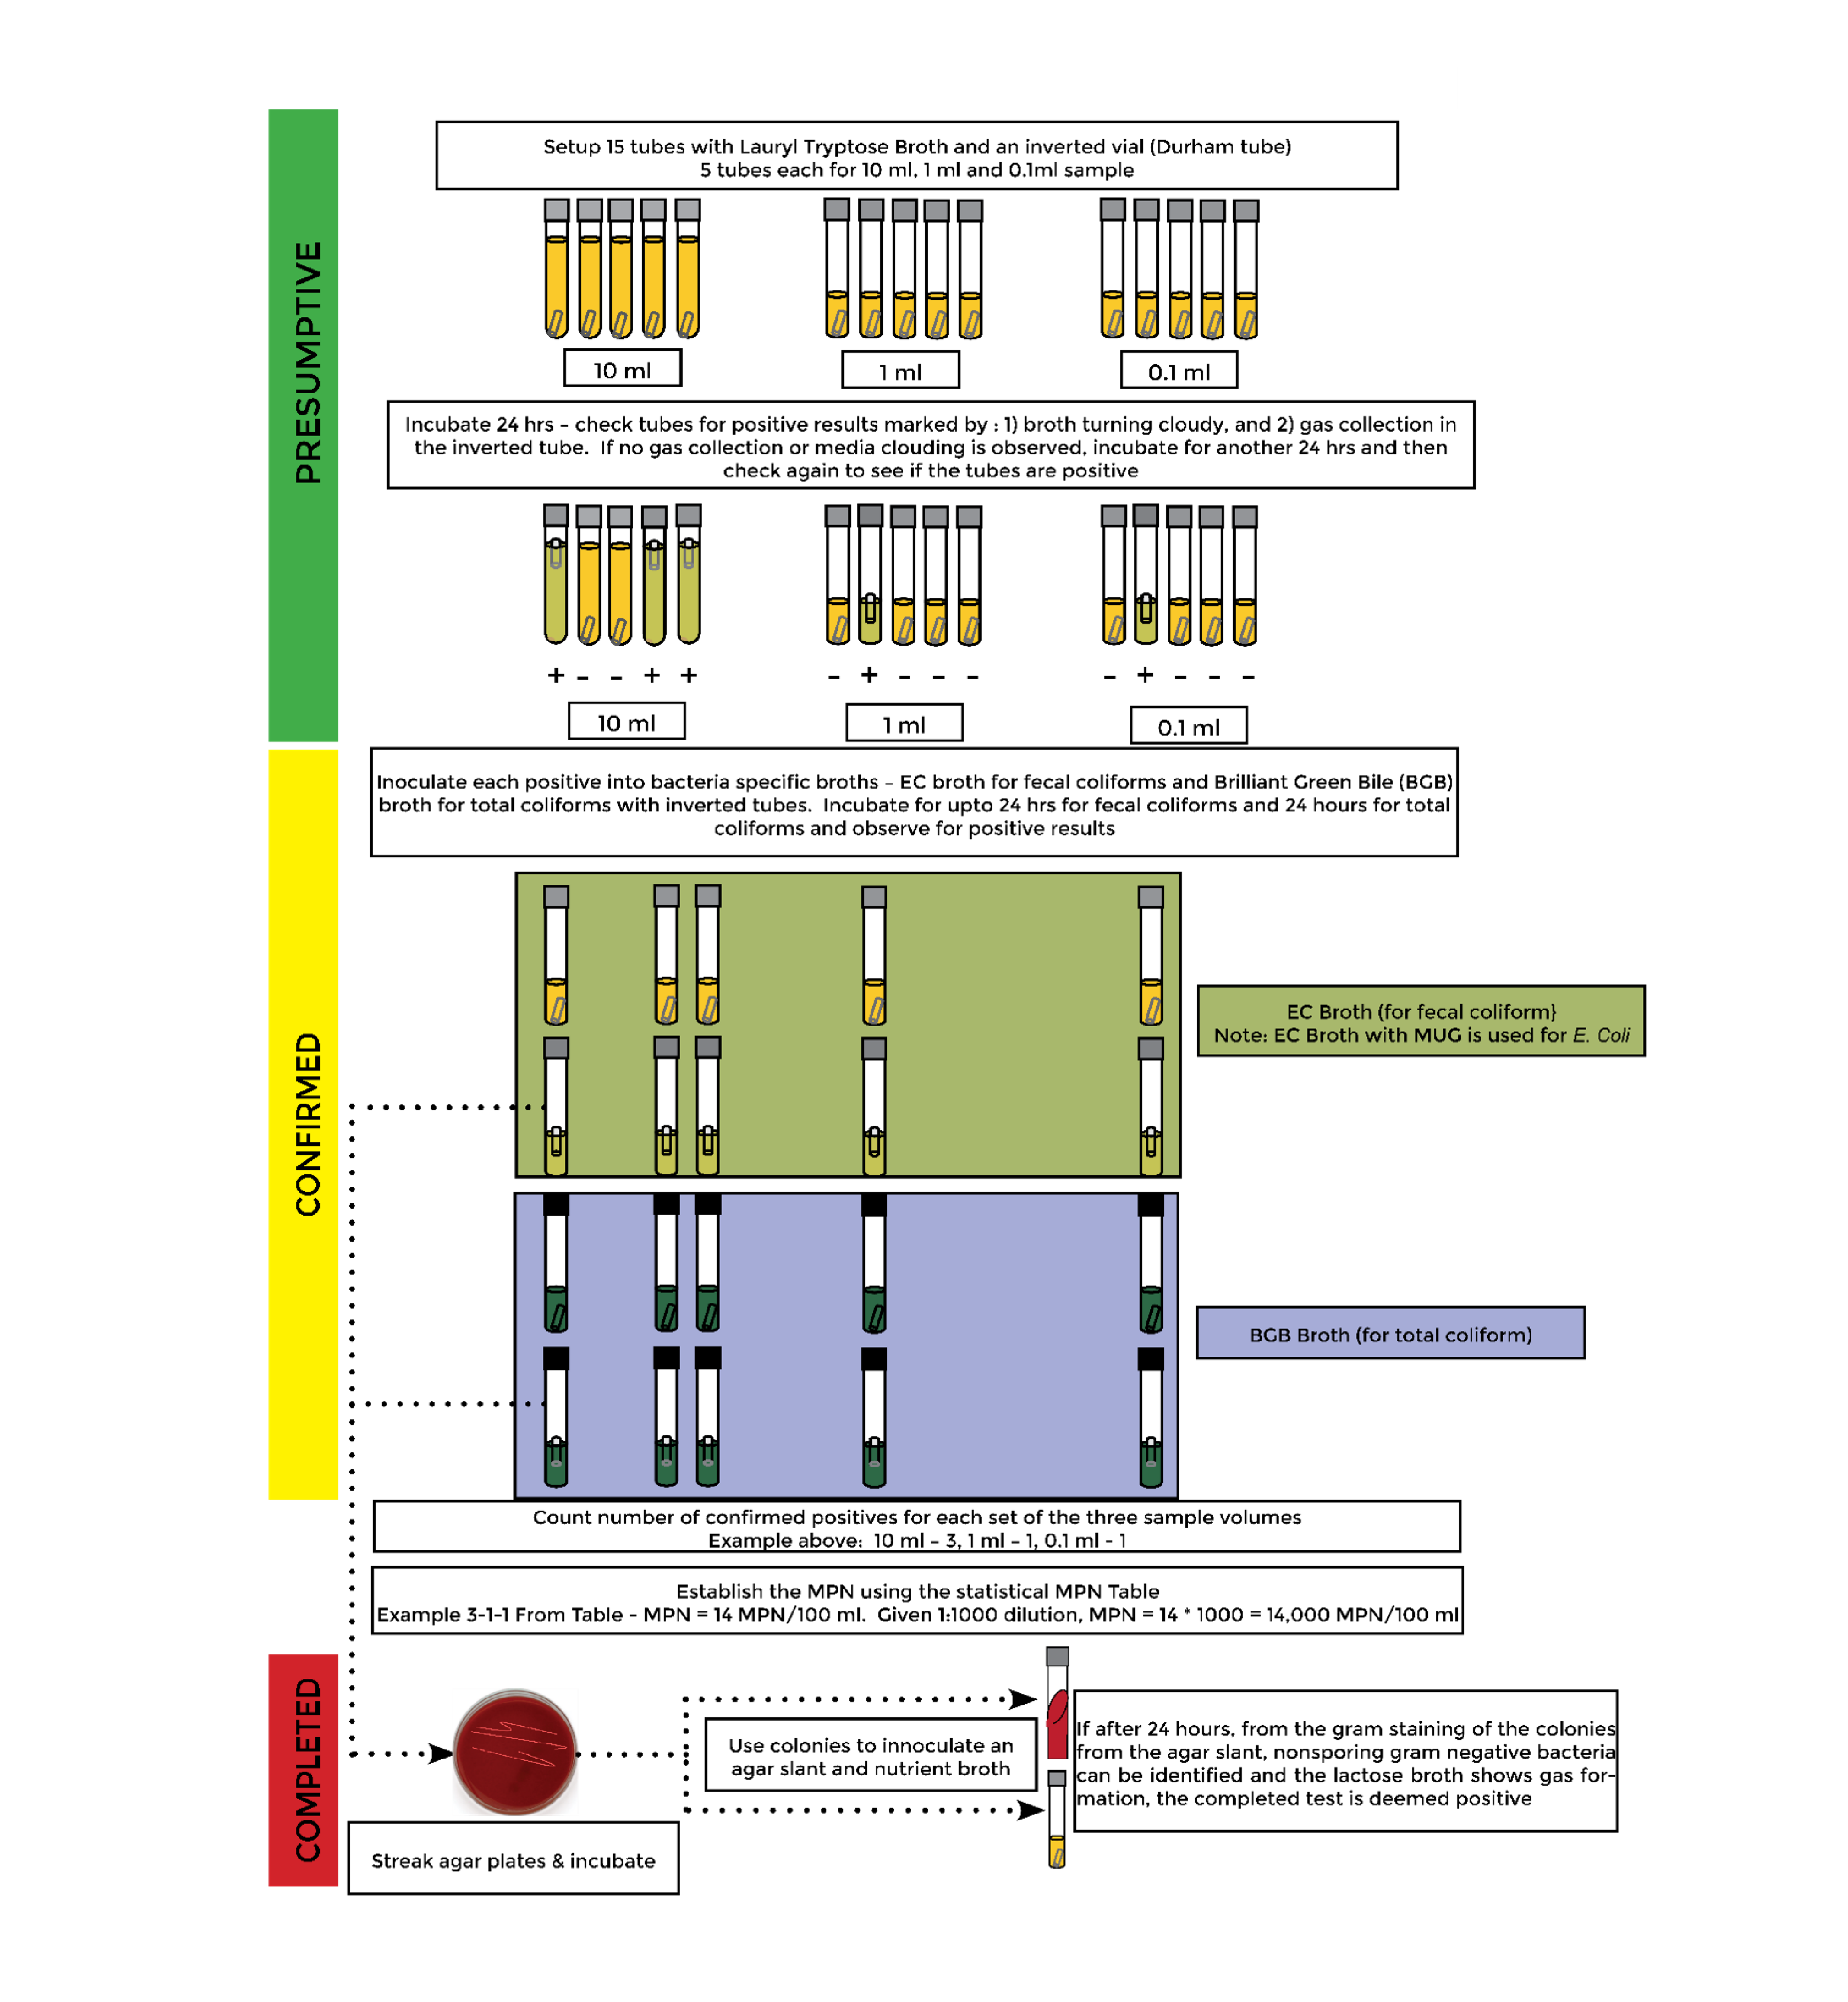
\includepdf[]{WaterMTF.pdf}
%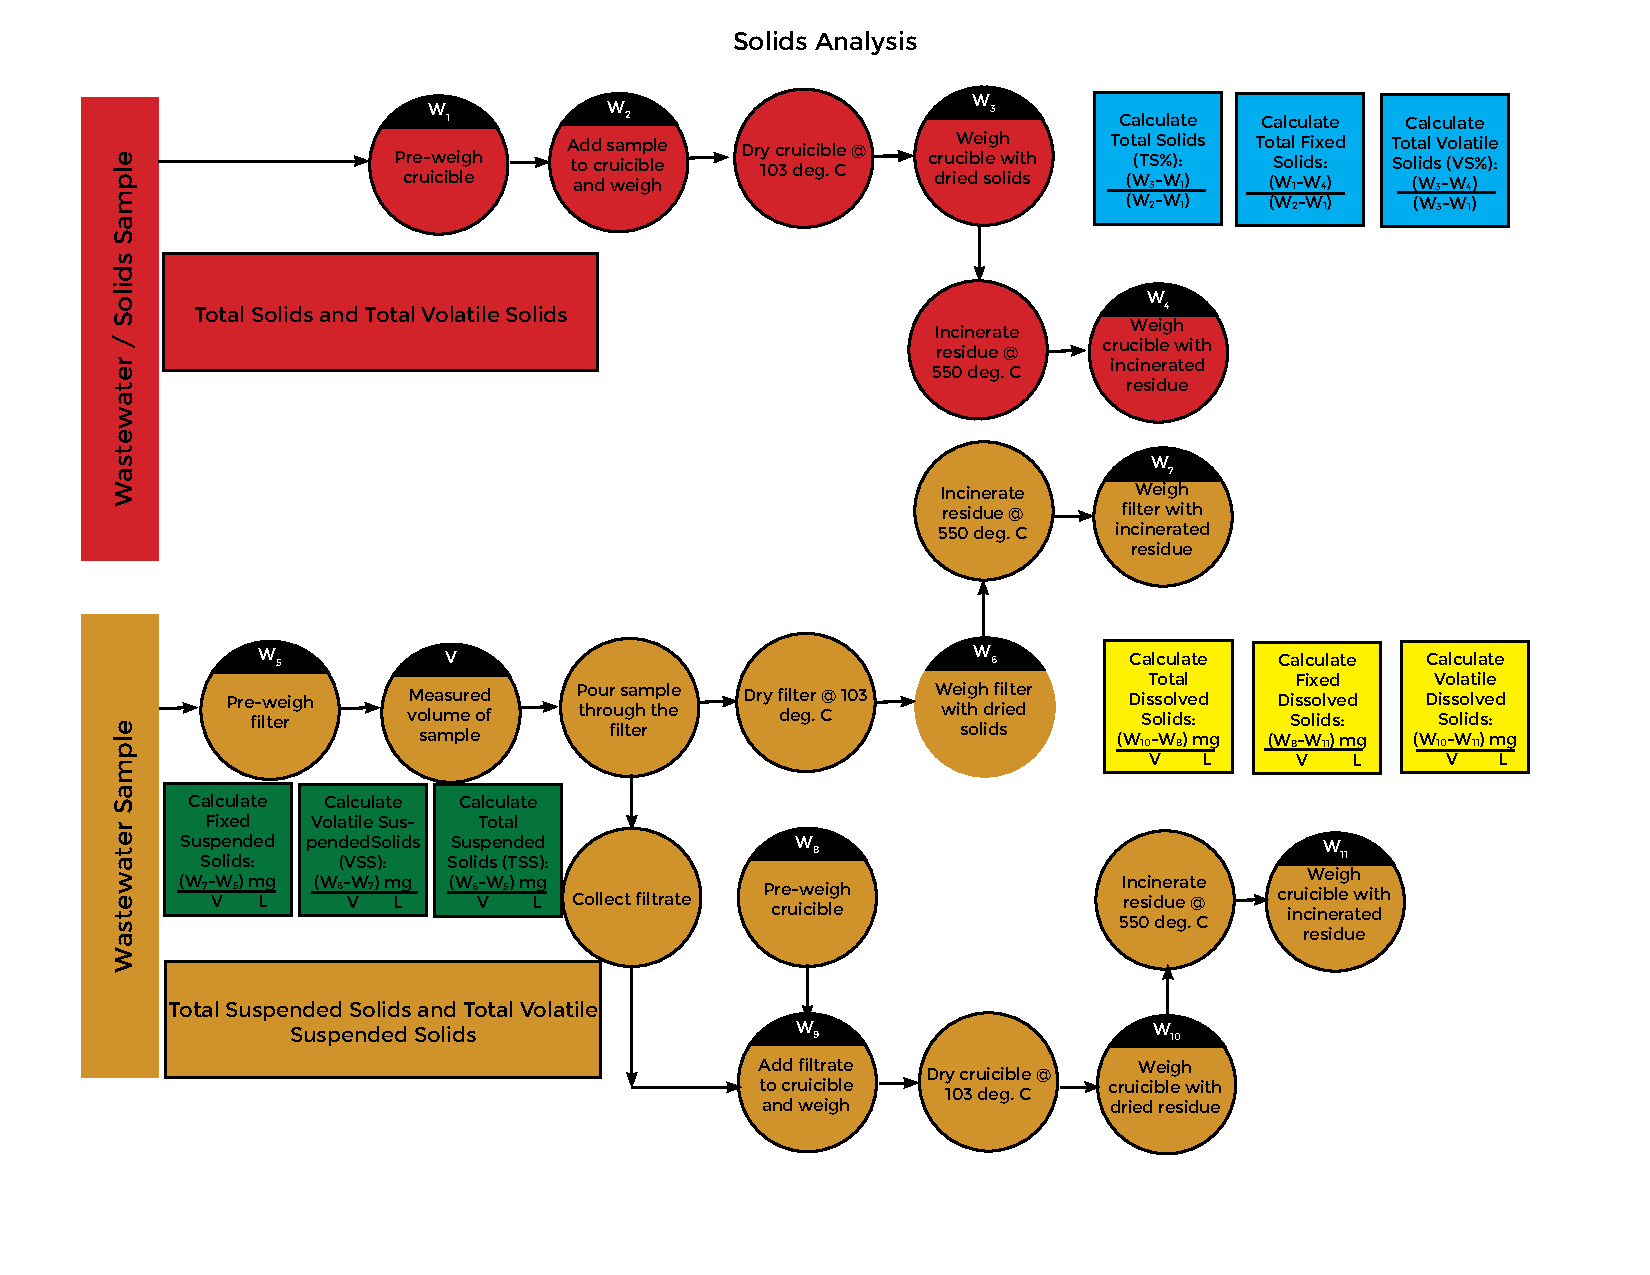
\includegraphics[scale=0.69]{LaboratorySolidsAnalysis4_01.pdf}
% \end{center}
% \end{landscape}
\begin{figure}[H]
\begin{center}
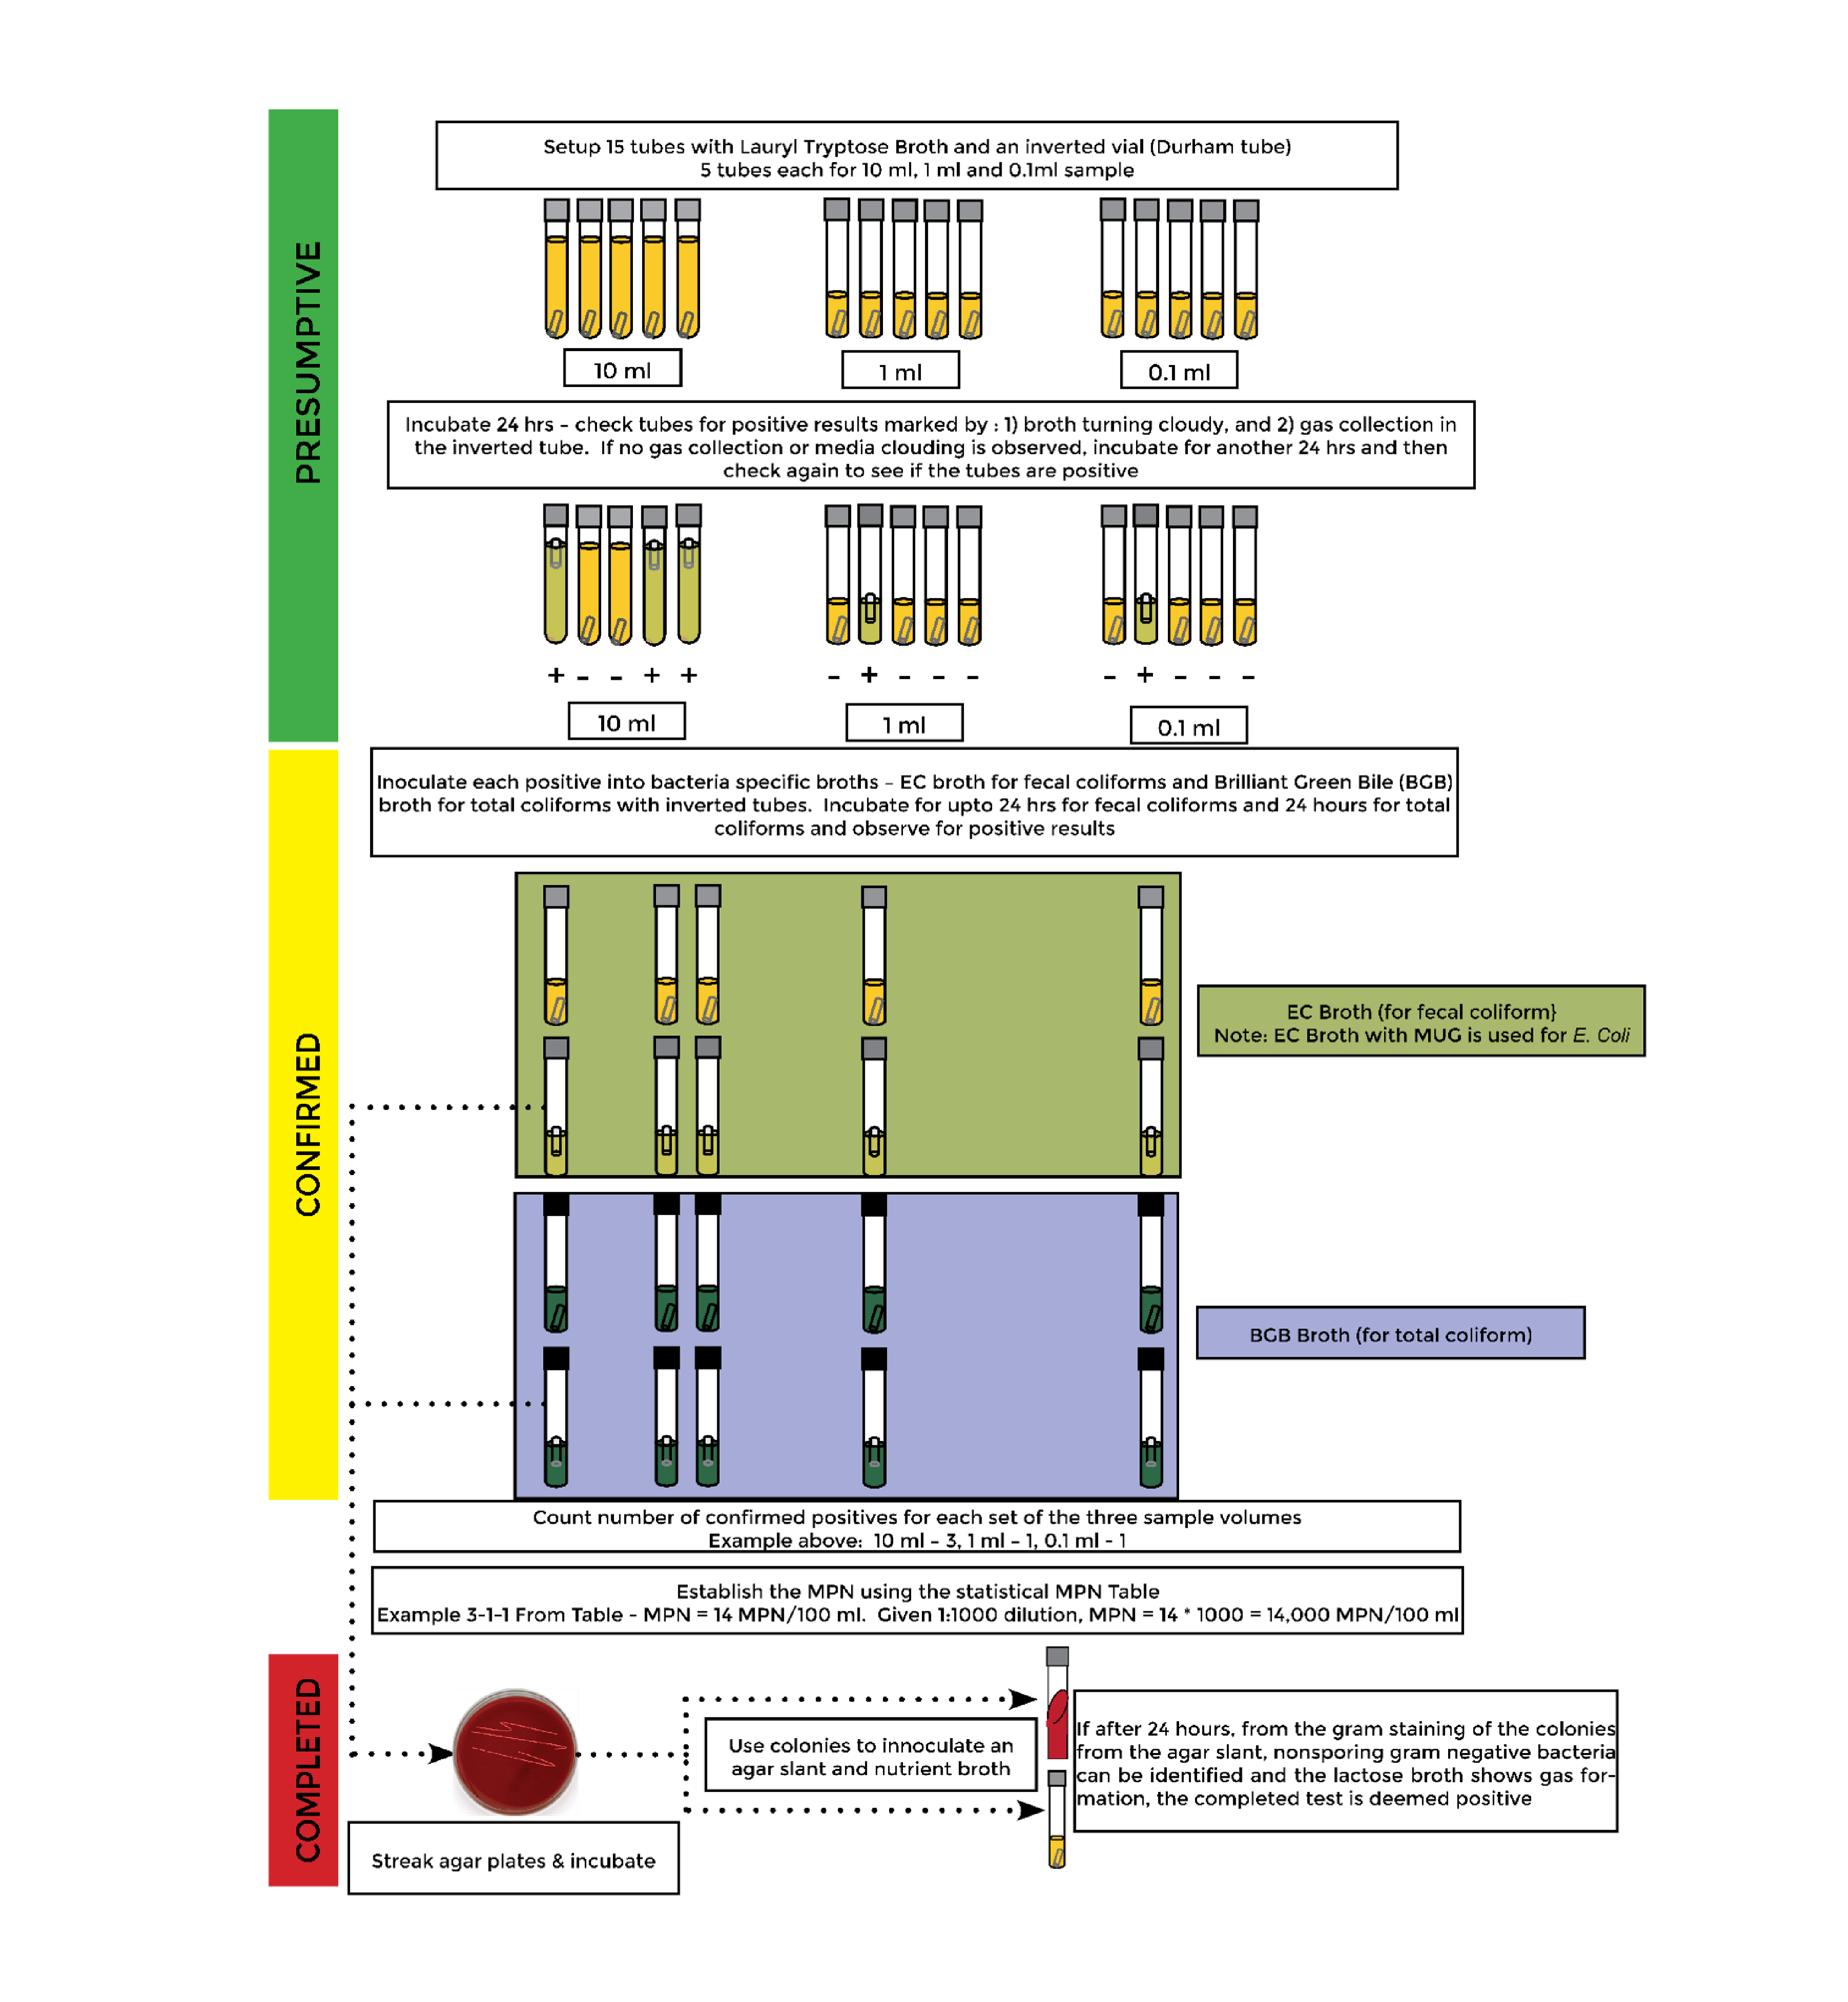
\includegraphics[scale=0.25]{WaterMTF}
\caption{Multiple tube fermentation}
\end{center}
\end{figure}
%\begin{figure}
%\begin{center}
%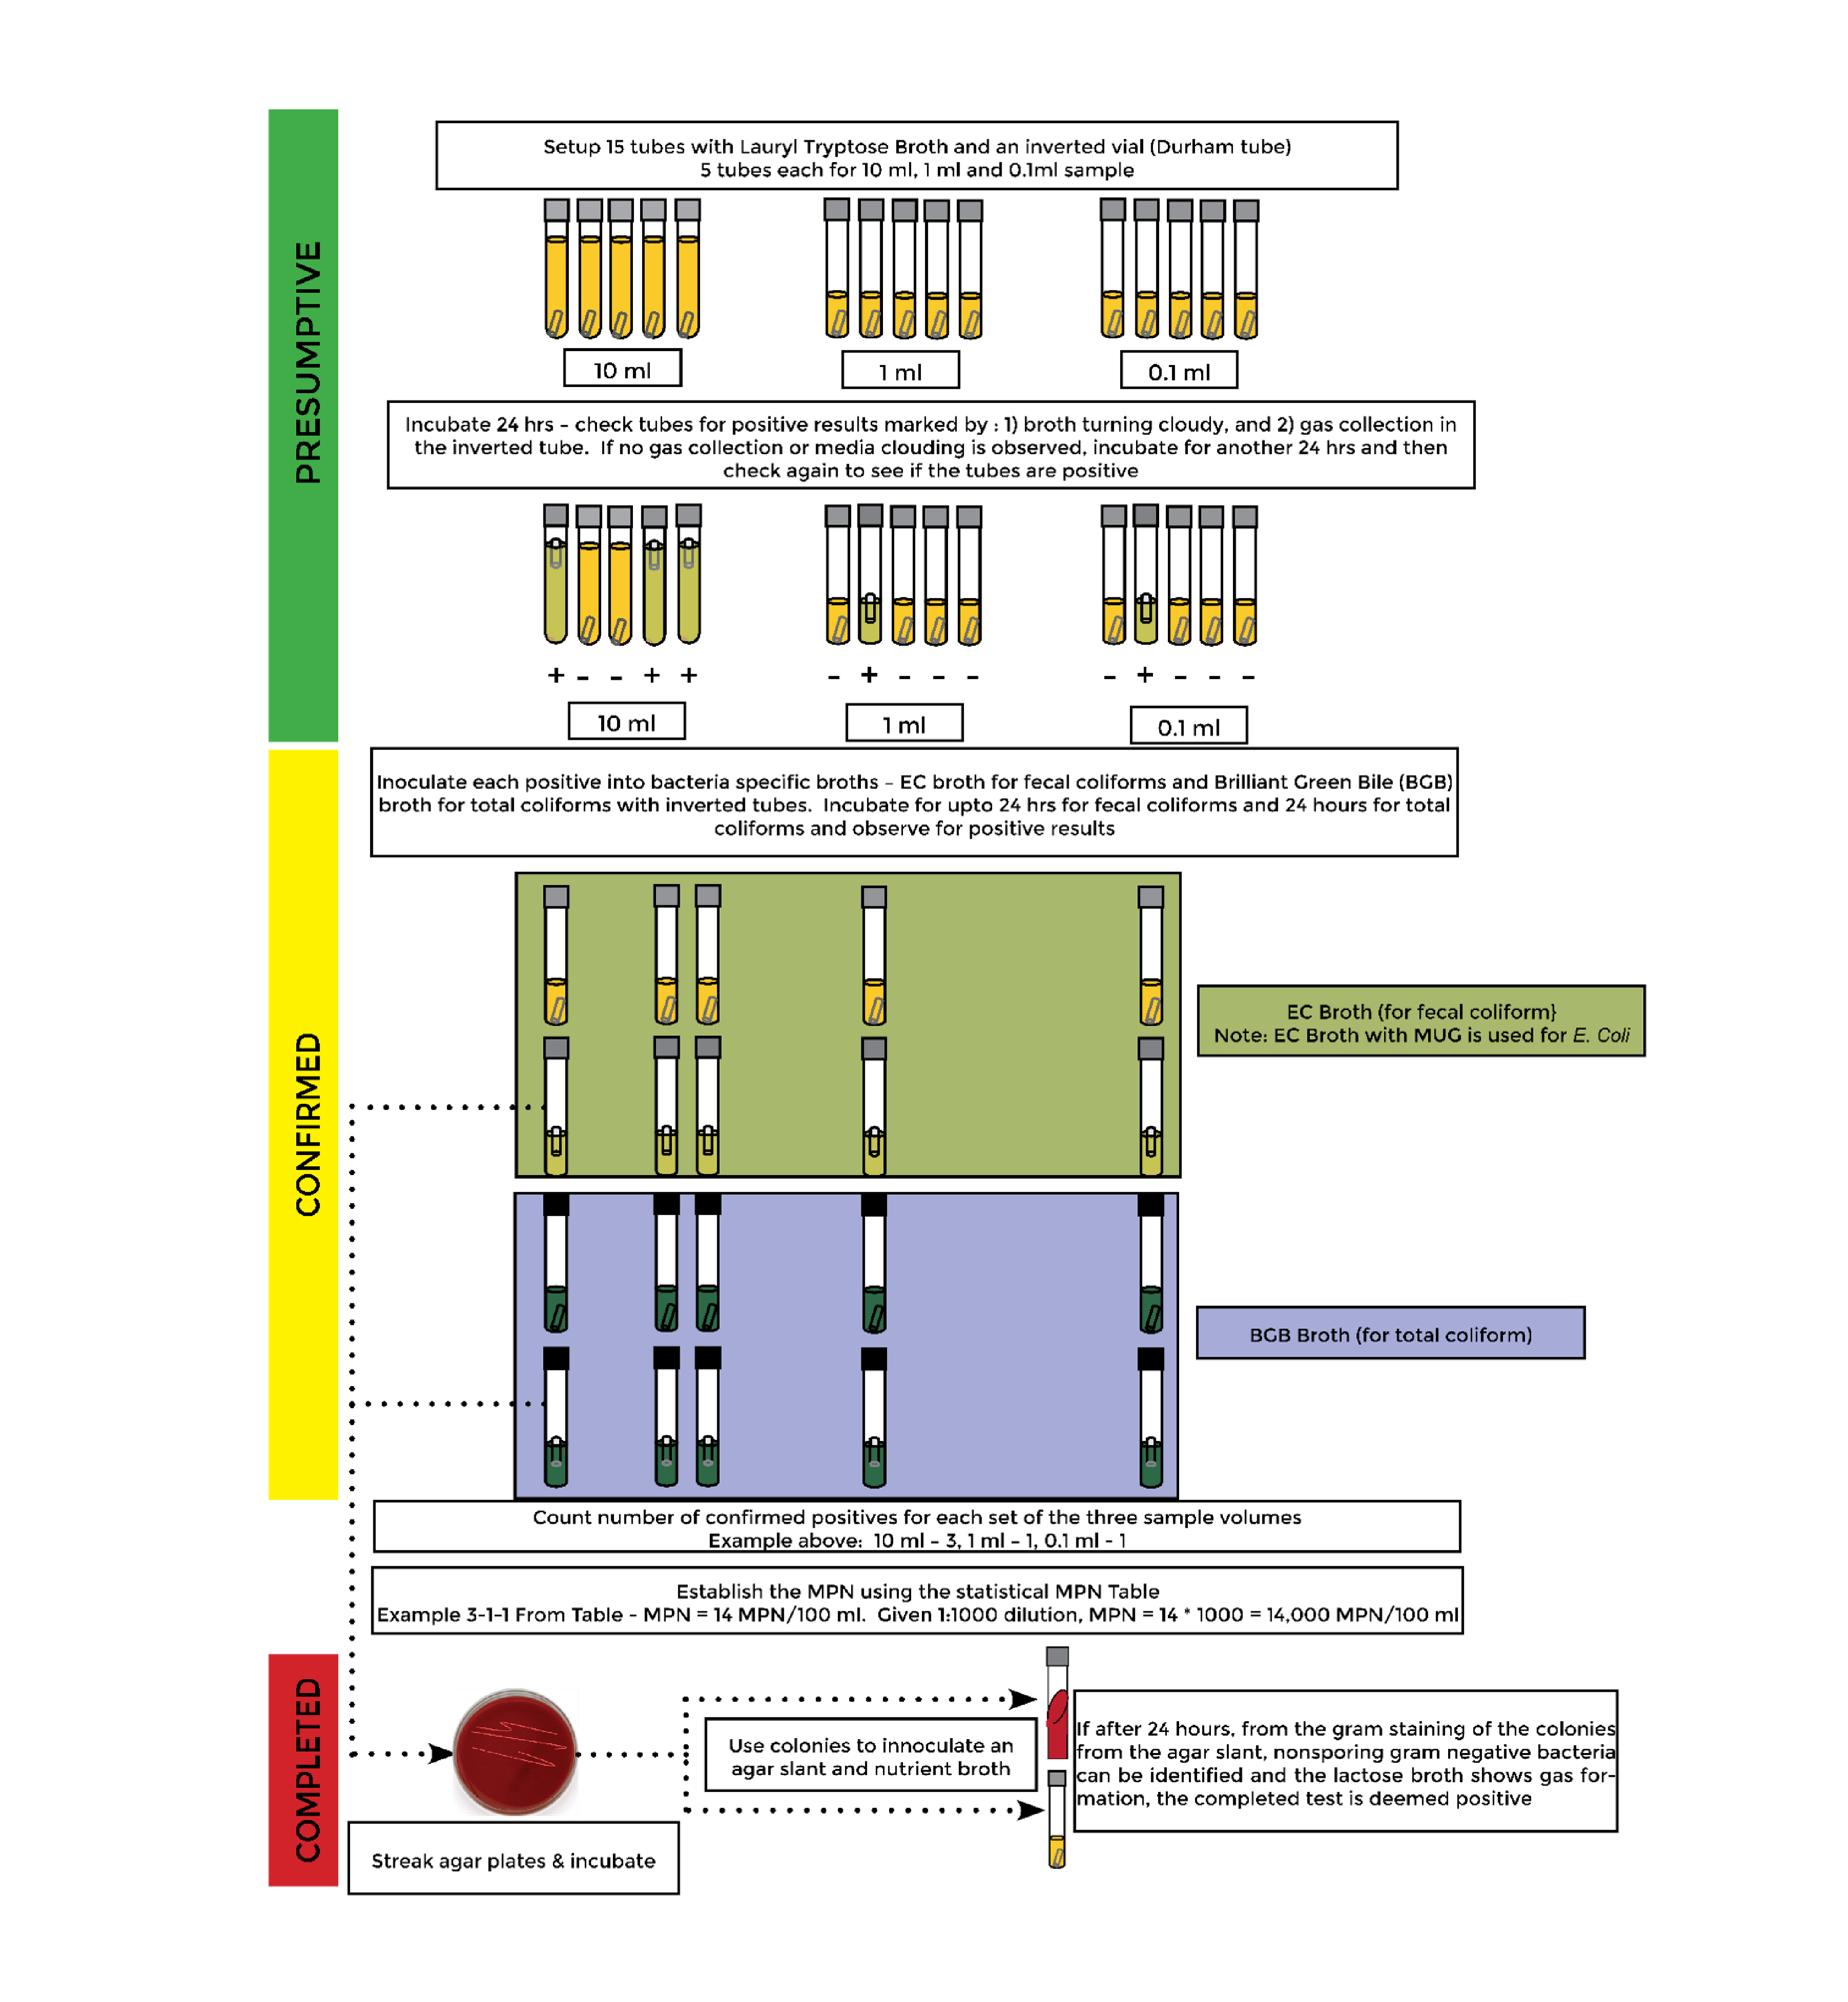
\includegraphics[scale=0.3]{WaterMTF}
%\end{center}
%\end{figure}
\thispagestyle{empty}
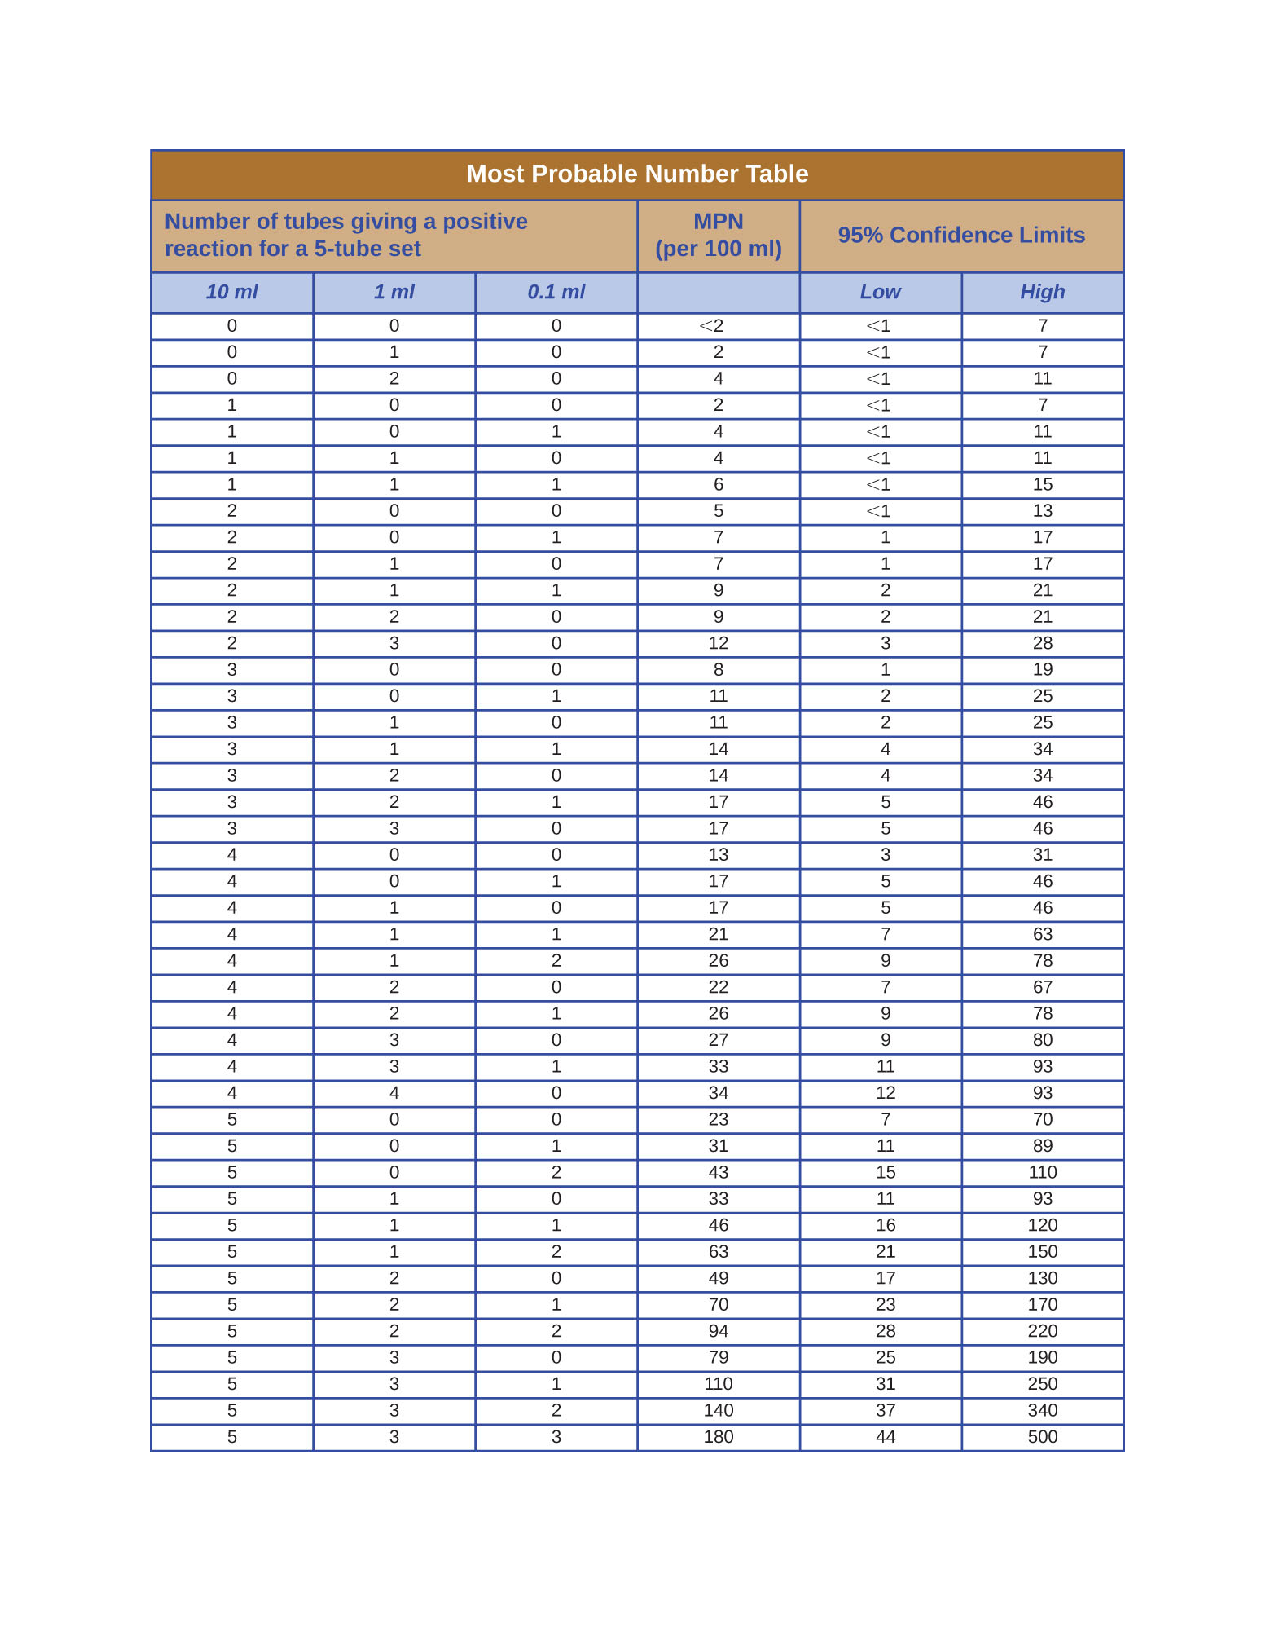
\includepdf[]{MTFTable.pdf}


\newpage

\subsection{Presence - absence (P-A) method}\index{Microbial testing!Presence-absence (P-A) method}
\begin{itemize}
\item Presence - Absence Method below is to assess the presence or absence of bacteria as required by the Revised Total Coliform Rule.
\item The Presence - Absence (P-A) Method for total coliform is based on two premises:
\begin{enumerate}
\item No coliform bacteria should be present in 100 mL of drinking water, and
\item If one viable cell is present it will multiply to give a population of cells that will ferment lactose to produce acid and gas.
\end{enumerate}

\item P-A Method is a simple modification of the multiple tube (MPN) method. P-A broth contains lactose and a pH indicator, which will change from purple to yellow if lactose is fermented and acid is produced. To this P-A broth, the compound \textbf{MUG} has been added. This initially colorless compound can be hydrolyzed by the E. coli to form a compound that fluoresces under long UV light (336 nm). Observing for fluorescence emission using a long-wave (e.g., 365 nm) UV lamp is a sensitive way to confirm the presence of E. coli in water samples.
 
\item The procedure involves addition of 100 ml of sample to 50 ml of sterile P-A broth and then incubating the inoculated broth at 35\degree{C} and inspected after 24 and 48 hours. Upon incubation, a positive result is indicated by the formation of a distinct yellow coloration of the media and/or gas formation which is indicated by foaming of the media upon gentle shaking of the bottle. 

\item Besides the P-A broth, the Colilert test enzymes (used in the above Quanti-Tray test) can be used to test for the Presence-Absence of coliforms.  The colilert enzyme is added to 100 ml water sample in a sterile, non-fluorescing vessel and incubated at 35\degree{C} for 24 h. The results are read at 24 h (before 28 h) and compared against the comparator. If no yellow color, the test is negative, If the sample has a yellow color equal to or greater than the comparator, the presence of total coliforms is confirmed. If yellow, check for blue fluorescence by placing a 6W, 365 nm UV light within 5 inches of the sample. If blue fluorescence is greater or equal to the fluorescence of the comparator the presence of E. coli is confirmed. 
\end{itemize}

\subsection{Heterotrophic plate count (HPC) }\index{Microbial testing!Heterotrophic plate count (HPC)}
\begin{itemize}
\item HPC test - also known as Standard Plate Count is used to measure the overall bacteriological quality of drinking water.
\item  It measures colony formation of heterotrophic bacteria present on culture media. HPC testing indicates the culturable organisms present, which could be as low as 1\% of the total bacteria present. 
\item Heterotrophs are a group of microorganisms including bacteria, molds and yeasts, that use organic carbon sources to grow and can be found in all types of water. Majority of bacteria found in drinking water systems are considered heterotrophs.
\item As all heterotrophic organisms are not pathogens and all pathogens are not heterotrophic, HPC results are not an indicator of water safety.
\item There is no maximum acceptable concentration of HPC in drinking water. However, increases in HPC concentrations above baseline levels are considered undesirable.

\item High HPC counts indicate ideal conditions for bacterial regrowth and should be corrected. Bacterial regrowth can lead to pipe corrosion, encourage slime growth, increase the need for disinfectants, cause foul-tasting water, and harbor secondary respiratory pathogens (ex. Legionella). Thus, HPC can be used as a marker for the underlying causes of some aesthetic problems

\item Methods used for routine testing of heterotrophic bacteria are
\begin{enumerate}
\item Pour plate method: \index{Microbial testing!Heterotrophic plate count (HPC)!Pour plate method}In this method, the liquid sample is poured into the petri dish before the solidification of the agar medium. After solidification, colonies grow both inside and on the surface of the medium.
\item Spread plate method \index{Microbial testing!Heterotrophic plate count (HPC)!Spread plate method}: Here the water sample is spread evenly over the surface of an agar plate medium.  A successful spread plate will have a countable number of isolated bacterial colonies evenly distributed on the plate.
\item Membrane filtration method \index{Microbial testing!Heterotrophic plate count (HPC)!Membrane filtration method}: This test uses a membrane filter is used to capture the bacteria as the water sample is filtered through it.  The filter is placed on an absorbent pad (in a petridish) saturated with a culture medium suitable for heterotrophe growth.
\end{enumerate}

\end{itemize}

\subsection{Other coliform quantification tests}
\ul{Membrane Filtration Method}\index{Microbial testing!Membrane filtration}
Membrane filtration (\textbf{MF}) is a faster way to estimate bacterial populations in water.  In this method, an appropriate sample volume is passed through a membrane filter with a pore size small enough (0.45 micron) to retain the bacteria present. The filter is placed on an absorbent pad (in a petri dish) saturated with a culture medium that is selective for coliform growth. The petri dish containing the filter and pad is incubated, upside down, for 24 hours at the appropriate temperature. After incubation, the colonies that have grown are identified and counted using a low power microscope. A MUG medium is used for E- Coli.  If E. Coli is present, it will make the MUG fluorescent when viewed in UV light. 


\begin{figure}[!htb]
    \centering
       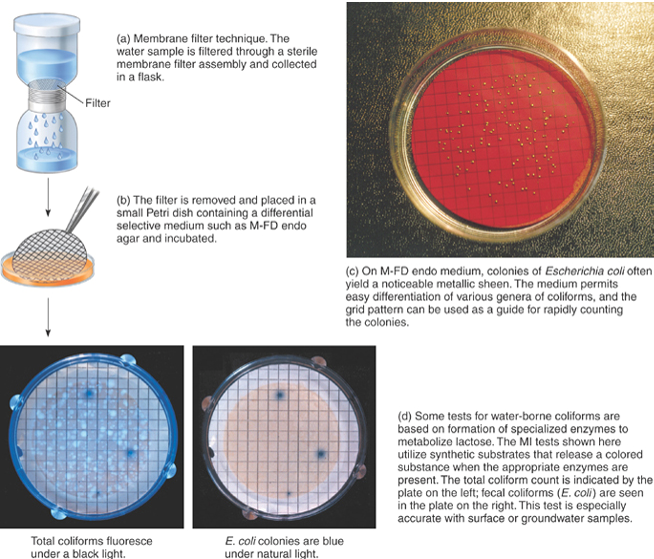
\includegraphics[width=\linewidth]{LaboratoryMembraneFiltration}
        \caption{Multiple tube fermentation}
    \end{figure}
    
\ul{Quanti-trays tests}\index{Microbial testing!Quanti-trays tests}

This test used for the detection and quantification of specific microorganisms is being used increasingly mainly because it is a quicker test than the MTF.  Colilert and Enterolert \index{Microbial testing!Colilert} are the quanti tray based tests for E. Coli and Enterococcus.  This method involve the use of specific enzymes and overcomes the drawbacks of the MTF which include false positives and negatives due to the more generic nature of the media used.
\begin{figure}[!htb]
    \centering
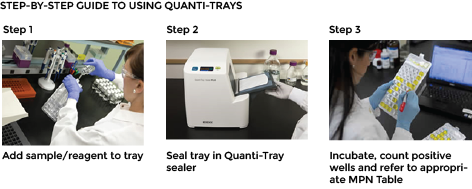
\includegraphics[width=\linewidth]{LaboratoryQuantiTray}
\caption{Quanti-trays test}
\end{figure}

\section{Sampling}\index{Sampling}

		\begin{itemize}
			\item Field or laboratory measurement of a certain parameter is critical in water treatment and distribution operations to obtain information about characteristics of water.
			\item A sample is a small part of the whole representing the whole.  Thus, a sample needs to be such that it truly represents the entire population – which could be either a treatment process stream or what is provided to the end user.
			\item As not all water is analyzed, a sample obtained for analysis must “represent” varying:
			\begin{itemize}
			\item Locations:  Locations should be representative of the majority of their portion of the Distribution System. Unusual locations should be avoided, as they are not indicative of the system as a whole.  Such locations are often monitored, but not as part of the routine plan.

			\item Time periods: Time period samples include:
			\begin{itemize}
			\item Grab: \index{Sampling!Grab} Sample taken in a single moment of time.
			\item Composite: \index{Sampling!Composite} Several portions collected over time and/or space.
			\item Continuous

			\end{itemize}
		\end{itemize}
		\end{itemize}


\subsection{Sampling methods}\index{Sampling!Sampling methods}

\subsubsection{Grab samples}\index{Sampling!Grab samples}
				\begin{itemize}
					\item A grab sample is a sample collected at a specific spot at a site over a short period of time.  
					\item Grab sampling allows for instantaneous analysis of parameters such as pH, dissolved oxygen, chlorine residual, temperature and other parameters which change rapidly with time.
					\item A grab sample represents a snapshot of space and time of a process stream.
					\end{itemize}

\subsubsection{Composite Samples}\index{Sampling!Composite Samples}
				\begin{itemize}
					\item A composite sample is a collection of discrete samples are combined over a certain period or space and therefore represent the average performance of a treatment plant or a process during the collection period.\\  
					\item Composite sampling can be either based on:
					      
					      1. constant time interval (time-proportioned sampling)\index{Sampling!Composite!time-proportioned sampling}\\
					      2. constant volume interval (flow-proportioned sampling), \index{Sampling!Composite!flow-proportioned sampling}and\\
					      3. treatment process space - includes samples taken at different depths \index{Sampling!Composite!depth sampling}\\
					      
					\item Composite samples are typically collected using automated samplers which can be programmed to collect samples at preset time intervals – for time proportional sampling.
					\item Time and space composite samples are collected by adding equal volumes of samples collected from different times or locations.  
					\item Flow proportional composite samples comprise of volume of each subsample based on flow.\\  
				\end{itemize}
	\begin{figure}			
			\begin{center}
				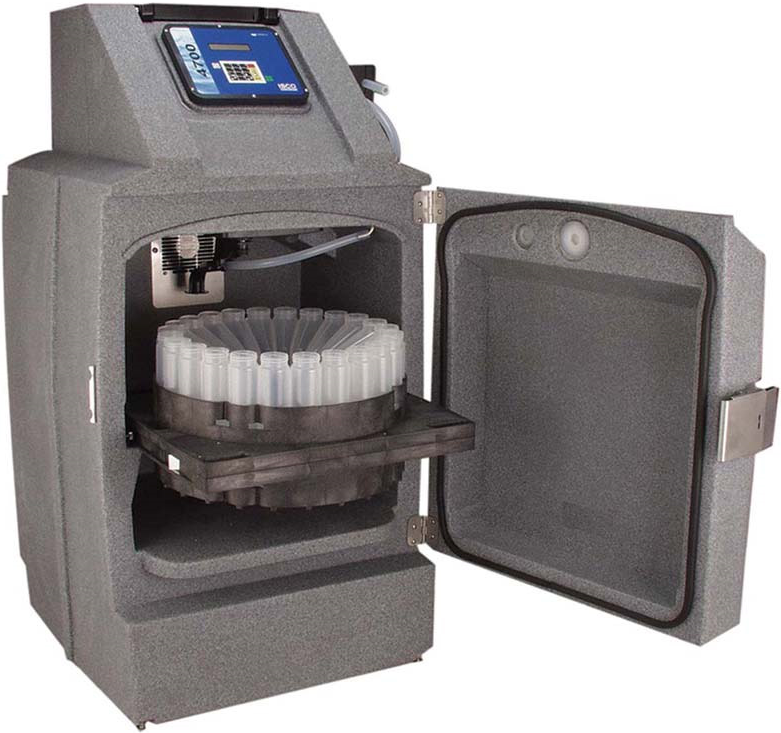
\includegraphics[scale=0.2]{Autosampler} \hspace{2cm} 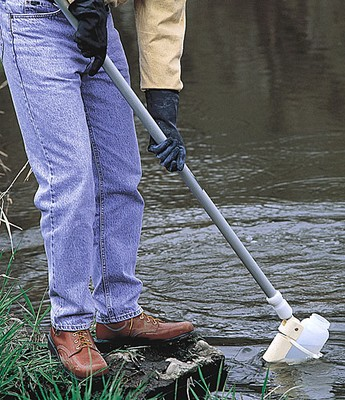
\includegraphics[scale=0.37]{Grabsampler}\\
			\end{center}
			\hspace{2.3cm} Automated Sampler \hspace{2.0cm} \parbox{\textwidth}{Grab Sampling Using a Long Handle Dipper}\\
\end{figure}
\subsection{Sampling precautions and protocols}\index{Sampling!Precautions and protocols}
			\begin{itemize}
				\item Samples should represent the major portion of the process or the process stream and should be taken from places where the mixing is thorough, avoiding dead spots and areas of heavier or lighter loadings. 
				\item The collected sample is invariably exposed to conditions very different from the original source and is subject to change due to chemical and microbiological activity.  
				\item Thus, in order to ensure integrity of sample, sample preservation techniques specific to the analysis to be performed is needed.  
				      \begin{itemize}
				      	\item The preservation technique should not only allow for stabilizing the parameter to be analyzed, it should also not interfere with the analyses.  
				      	\item The common preservation techniques involve use of proper containers, temperature control, addition of chemical preservatives, and observance of the recommended maximum sample holding time.
				      \end{itemize}
				      \item Samples cannot be held indefinitely prior to lab analysis
\item  Laboratories used for testing must be approved by Environmental Laboratory Accreditation Program {ELAP} \index{Environmental Laboratory Accreditation Program (ELAP)} and must use Standard Methods.
\item Chain-of-custody \index{Chain-of-custody}ensures sample integrity from collection to data reporting Important for sample control when litigation is involved Must be under a person’s physical possession, within sight, or secured in a restricted area Receipt and logging of sample at lab Complete documentation from collection to report
\item Sample Containers:
\begin{itemize}
\item Typically plastic or glass
\item Use proper material for analysis
\item Use glass for all organic and odor analyses
\item Use plastic for metals
\item Bacteriological sample containers must be sterile
\end{itemize}
\end{itemize}

\subsection{Microbial sampling}\index{Sampling!Microbial sampling}
\begin{itemize}
\item Always collected as a grab.
\item The sample is obtained from a steady, pencil-width stream from a cold water fixture, only after it has been in a wide open setting and  water to run a minimum of five minutes to flush out the bacteria from the surface. 
\item A clean, sterile borosilicate glass or plastic bottle containing sodium thiosulfate is used. Sodium thiosulfate is added to remove residual chlorine which will kill the microorganisms during transit. If the sample is not preserved or maintained under proper conditions until the test is conducted in the laboratory, the test would provide erroneous results
\item Samples must be refrigerated if they cannot be analyzed within 1 hour of collection
\item Samples must be handled with care to prevent contamination and adverse conditions such as prolonged exposure to direct sunlight
\item Maximum holding time for state or federal permit reporting purposes is 6 hours
\item Number of samples collected depends on number of customers served/and is according to the approved sample siting plan.
\item The volume for coliform compliance sample must be at least 100ml and no more than 120ml. 
\item Sealed and sterilized sampling bottles - typically, 120 ml with 100 ml marked to provide space for air is used.
\item Sodium thiosulfate or some other de-chlorinator \index{Chlorine disinfection!Dechlorination}is pre-added to the sampling bottle. A dechlorinator is critical to ensure any chlorine residual is removed from the sample collected.
\item The faucet is opened to obtain a continuous flow of the size of a pencil, the faucet should not be opened under a strong flow as  that could potentially dislodge loose particles/slime growth in the mains.
\item When the cap is opened to collect the sample, care needs to be taken to ensure the cap is not contaminated.
\item Fill the bottle to the marked fill-line leaving an air gap - do not overfill.
\item The capped bottle should be placed in an iced container and transported to the laboratory as soon as possible.
\item Follow chain-of-custody \index{Chain-of-custody}and send the bottles to the lab with paperwork.
\item In the laboratory, the samples must be kept at 4\degree{C} or 39\degree{F} and must be analyzed preferably within 8 hours and never to exceeding 24 hours.
\item The analytical results shall be reported in terms of the presence or absence of total coliforms and E. coli, in the sample, whichever is appropriate.
\item Monthly sampling results must be submitted to the regulatory agency per established scheduled.
\item Records of bacteriological sampling must be kept for five years \index{Bacteriological sampling records}.
\item Repeat sampling:  If the result is positive a minimum three samples need to be taken, one from the original point, one up-stream and one from downstream of the original sample collection site within 24 hours after the result notification from the laboratory.
\item False positive means that the sample when tested is found to be contaminated but
actually the water is safe.
\item False negative means samples are found to be safe; even though the water is
- unsafe to drink. This can lead to outbreak of diseases and cause customers to lose confidence in their drinking water supplier. This harms the customer. \index{False negative/positive}
\end{itemize}
\newpage
\subsection{Summary of sampling requirements}\index{Sampling!Summary of sampling requirements}\index{Sampling!Preservative}\index{Sampling!Holding time}
\begin{table}[h!]
\begin{tabular}{|p{4cm}|p{3cm}|p{4cm}|p{3cm}|}
\hline
\multicolumn{1}{|c|}{\textbf{Parameter}}                                                   & \multicolumn{1}{c|}{\textbf{Container}}                                            & \multicolumn{1}{c|}{\textbf{Preservative}}                                                                                                                   & \multicolumn{1}{c|}{\textbf{Holding Time}}                          \\ \hline
\begin{tabular}[c]{@{}l@{}}Coliform, total or fecal,\\      in chlorinated water\end{tabular} & \begin{tabular}[c]{@{}l@{}}Sterile container    w/\\      thiosulfate\end{tabular} & Cool   to \textless{}10 °C.  Do not freeze                                                                                                                    & 8   hrs for source water compliance and 30 hours for drinking water \\ \hline
Giardia and   Cryptosporidium                                                              & 10   L plastic container                                                           & Cool   to \textless{}10  °C .  Do not freeze                                                                                                                    & 96   hours                                                          \\ \hline
Alkalinity, turbidity, solids                                                             , fluoride & Plastic or Glass                                                                   & Cool   to \textless{} 4 °C                                                                                                                                             & Method   dependent                                                  \\ \hline
Metals, general                                                                            & Plastic or Glass, Rinsed w/ 1:1 HNO$_3$                                               & Nitric   acid to pH \textless 2                                                                                                                              & 6 Months                                                            \\ \hline
Hardness                                                                           & Plastic or Glass                                                                   & Nitric   acid to pH \textless 2                                                                                                                              & 6 Months                                                            \\ \hline
pH                                                                                         & Plastic or Glass                                                                   & None                                                                                                                                                         & Analyze in 15 min                                                    \\ \hline
Nitrogen and   phosphorous compounds                                                       & Plastic or Glass                                                                   & Sulfuric acid to   pH\textless{}2                                                                                                                            & 28 days                                                             \\ \hline
VOCs, TTHMs                                                                                & Glass bottle                                                                       & Sodium thiosulfate or   ascorbic acid if sample is chlorinated and hydrochloric acid (HCl) to pH \textless 2  and cool to  \textless 4 °C  but do not freeze & 14 days                                                             \\ \hline
\end{tabular}
\caption{Summary of sampling requirements for key parameters}\index{Sampling!Summary of requirements}
\end{table}






\chapterimage{QuizCover} % Chapter heading image

\chapter*{Chapter 3 Assessment}
% \textbf{Multiple Choice}
\section*{Chapter 3 Assessment}
\begin{enumerate}[1.]

\item Hard water contains an abundance of\\
a. sodium\\
b. iron\\
c. lead\\
d. calcium carbonate\\
\item A specific class of bacteria that only inhibit the intestines of warm-blooded animals is referred to as?\\
a. Eutrophic\\
b. Grazing\\
c. Salmonella\\
d. Fecal coliform\\
e. pathogenic\\
\item Water with a pH of 8.0 is considered to be\\
a. acidic\\
b. basic or alkaline\\
c. neutral\\
d. undrinkable\\
\item Over which water quality indicator do operators have the greatest control?\\
a. alkalinity\\
b. pH\\
c. temperature\\
d. turbidity\\
\item Which piece of laboratory equipment is used to titrate a chemical reagent?\\
a. graduated cylinder\\
b. burette\\
c. pipet\\
d. Buchner funnel\\
\item Which pH range is generally accepted as most palatable (drinkable)?\\
a. 6.5 to 8.5\\
b. 4.5 to 6.5\\
c. 8.5 to 9.5\\
d. 9.5 and above\\
e. all of the above\\
\item Which of the following conditions is favorable for the rapid growth of algae?\\
a. plant nutrients\\
b. high $\mathrm{pH}$ and water hardness\\
c. low temperatures and low dissolved oxygen\\
d. high alkalinity and water hardness\\
\item Which of the following is the name given for a turbidity meter that has reflected or scattered light off suspended particles as a measurement?\\
a. Hach colorimeter\\
b. spectrophotometer\\
c. Wheaton bridge\\
d. Nephelometer\\
\item Water hardness is the measure of the concentrations of and dissolved in the water sample.\\
a. iron, manganese\\
b. nitrates, nitrites\\
c. sulfates, bicarbonates\\
d. calcium \& magnesium carbonates\\
e. ferric chlorides and polymers\\
\item The electrical potential required to transfer electrons from one compound or element to another is commonly referred to as\\
a. oxidation-reduction potential (ORP)\\
b. voltage potential $(\mathrm{OHM} / \mathrm{P})$\\
c. resistance-impedance potential\\
d. microMho differential\\
\item Water has physical, chemical, and biological characteristics. Which of the following is a physical characteristic?\\
a. Coliform\\
b. Turbidity\\ 
c. Hardness\\
d. All the above\\
\item Tastes and odors in surface water are most often caused by:\\
a. clays\\
b. hardness\\
c. algae\\
d. coliform bacteria\\
\item Which of the following elements cause hardness in water?\\
a. sodium and potassium\\
b. calcium and magnesium\\
c. iron and manganese\\
d. turbidity and suspended solids\\
\item When measuring for free chlorine residual, which method is the quickest and simplest?\\
a. DPD color comparator\\
b. Orthotolidine method\\
c. Amperometric titration\\
d. 1, 2 nitrotoluene di-amine method\\


\end{enumerate}



\part{Chapter 4}
\chapterimage{Water1.png} % Chapter heading image

\chapter{Drinking Water Regulations}

\begin{table}[H]
\begin{tabular}{| m{1cm} | m{15cm} |}
\hline
\multicolumn{2}{|l|}{\textbf{Expected   Range of Knowledge for Water Properties and Sources}}                                                                          \\ \hline
\multicolumn{2}{|l|}{\textit{Water   Distribution System Operator License Exams}}                                                                                      \\ \hline
D1 & Ability to read   a sample siting plan                                                                                    \\ \hline
D1 & Ability to take a   lead and copper sample                                                                                \\ \hline
D1 & Knowledge of acute   violations                                                                                           \\ \hline
D1 & Knowledge of CDPH   Water Quality regulations                                                                             \\ \hline
D1 & Knowledge of the   definition of MCL                                                                                      \\ \hline
D1 & Knowledge of the   major components of the SDWA                                                                           \\ \hline
D1 & Knowledge of the   purpose of the SDWA                                                                                    \\ \hline
D1 & Knowledge of Total   Coliform Rule reporting requirements                                                                 \\ \hline
D1 & Knowledge of Total   Coliform Rule sampling requirements                                                                  \\ \hline
D1 & Knowledge of when   public notification is required                                                                       \\ \hline
D2 & Ability to   differentiate between a primary and secondary MCL                                                            \\ \hline
D2 & Ability to recognize   MCL violations                                                                                     \\ \hline
D2 & Knowledge of AWWA   disinfection standards                                                                                \\ \hline
D2 & Knowledge of   Disinfection By-Product Rule sampling requirements                                                         \\ \hline
D2 & Knowledge of maximum   disinfectant residual level for chlorine                                                           \\ \hline
D2 & Knowledge of   reporting and recordkeeping requirements                                                                   \\ \hline
D3 & Knowledge of the   relationship between corrosion and lead/copper concentrations                                          \\ \hline
D3 & Knowledge of   Disinfection By-Product Rule MCL requirements                                                              \\ \hline
D3 & Knowledge of   Disinfection By-Product Rule reporting requirements                                                        \\ \hline
D3 & Knowledge of lead and   copper rule reporting requirements                                                                \\ \hline
D3 & Knowledge of lead and   copper sampling requirements                                                                      \\ \hline
D3 & Knowledge of public   notification requirements                                                                           \\ \hline
D3 & Ability to perform   damage assessment and recovery planning                                                              \\ \hline
D3 & Ability to train   personnel on emergency response procedures                                                             \\ \hline
D3 & Knowledge of   non-compliance penalties                                                                                   \\ \hline

\end{tabular}
\end{table}


\newpage



\begin{table}[H]
\begin{tabular}{| m{1cm} |m{15cm} |}
\hline
\multicolumn{2}{|l|}{\textbf{Expected   Range of Knowledge for Water Properties and Sources}}                                                                      \\ \hline
\multicolumn{2}{|l|}{\textit{Water   Distribution System Operator License Exams (Continued)}}                                                                  \\ \hline
D4 & Ability to recognize a lead and copper rule   violation                                                                   \\ \hline
D4 & Knowledge of notification paths (e.g.   newspaper, electronic)                                                            \\ \hline
D4 & Knowledge of required language to use                                                                                     \\ \hline
D5 & Knowledge of Air   Quality Management regulations                                                                         \\ \hline
D5 & Knowledge of O\&M   budget components (e.g. labor, professional services, supplies, energy,   water, capital improvement) \\ \hline
D5 & Knowledge of RWQCB   discharge requirements                                                                               \\ \hline
D5 & Knowledge of the   components of a budget (e.g. revenues, expenditures, risk management,   insurance costs, depreciation) \\ \hline
\multicolumn{2}{|l|}{\textit{Water   Treatment System Operator License Exams }}                                                                  \\ \hline
T1 & Knowledge of   disinfection residual requirements                                                                         \\ \hline
T1 & Knowledge of MCLs and   MRDLs of disinfectants                                                                            \\ \hline
T1 & Knowledge of drinking   water monitoring and reporting requirements                                                       \\ \hline
T1 & Knowledge of drinking   water regulations                                                                                 \\ \hline
T1 & Knowledge of   notification protocol and procedures                                                                       \\ \hline
T1 & Knowledge of NSF   Standards                                                                                              \\ \hline
T1 & Knowledge of operator   certification requirements                                                                        \\ \hline
T1 & Knowledge of Primary   and Secondary Drinking Water Standards                                                             \\ \hline
T1 & Knowledge of public   notification procedures                                                                             \\ \hline
T1 & Knowledge of record   keeping requirements                                                                                \\ \hline
T1 & Knowledge of   California Waterworks Standards                                                                            \\ \hline
T1 & Knowledge of the   Consumer Confidence Report (CCR)                                                                       \\ \hline
T1 & Knowledge of the   Disinfectants and Disinfection Byproduct Rule and amendments                                           \\ \hline
T1 & Knowledge of the   Groundwater Rule                                                                                       \\ \hline
T1 & Knowledge of the Lead   and Copper Rule                                                                                   \\ \hline
T1 & Knowledge of the   Surface Water Treatment Rule and amendments                                                            \\ \hline
T1 & Knowledge of the   Total Coliform Rule and amendments                                                                     \\ \hline
T1 & Ability to research   and interpret Maximum Contaminant Levels (MCLs)                                                     \\ \hline
T2 & Knowledge of   cryptosporidium action plan                                                                                \\ \hline
T2 & Knowledge of pending   regulations                                                                                        \\ \hline
T2 & Knowledge of   performance standards and removal requirements for surface water treatment                                 \\ \hline
T2 & Knowledge of the   Filter Backwash Rule                                                                                   \\ \hline
T2 & Knowledge of routine   sampling requirements                                                                              \\ \hline
T3 & Ability to administer   a regulatory compliance program                                                                   \\ \hline
T3 & Knowledge of permit   requirements for water operations                                                                   \\ \hline
T3 & Knowledge of pump to   waste discharge environmental regulations                                                          \\ \hline
T3 & Knowledge of   regulatory primacy issues                                                                                  \\ \hline
T3 & Knowledge of source   water replenishment processes                                                                       \\ \hline
T3 & Knowledge of the   Sanitary Survey process                                                                                \\ \hline
T4 & Knowledge of the role   of Regional Boards in managing contamination sources                                              \\ \hline
T4 & Knowledge of the   Source Water Assessment Program                                                                        \\ \hline
T4 & Knowledge of the   Watershed Survey process                                                                               \\ \hline
T4 & Knowledge of the   vulnerability assessment process                                                                       \\ \hline
\end{tabular}
\end{table}


\newpage






















\section{Drinking water regulations}\index{Drinking water regulations}
\begin{itemize}
\item Drinking water sources which include surface and groundwater sources have inherent vulnerabilities to contamination and regulations have been established to protect public health and safety.
\item Federal Safe Drinking Water Act (\textbf{SDWA}) \index{Safe Drinking Water Act (SDWA)} enacted in 1974 established national enforceable standards for drinking water quality and to guarantee that public water systems monitor water to ensure that it meets national standards. \\
\item The SDWA prescribes enforceable primary standards for five major categories of drinking water contaminants consisting of Inorganic Chemicals, Organic Chemicals, Radionuclides, Microorganisms, Disinfectants and Disinfection Byproducts.
\item The SDWA delegates responsibility for administering the provisions of
the act to the US Environmental Protection Agency (\textbf{USEPA}) \index{US Environmental Protection Agency (USEPA)}.
\item The enforcement of SDWA requirements is delegated by the USEPA to individual states
\item Individual states are provided the opportunity to set and enforce their own drinking water standards for public water systems if the standards are at a minimum as stringent as EPA's national standards.
\item A \textbf{primacy agency}is the agency with primary responsibility for implementing the SDWA. Most states and the U.S. territories have been approved to exercise primary responsibility in their jurisdictions. Exceptions are the state of Wyoming and the District of Columbia, which are implemented by EPA. 
\item In the SDWA, a \textbf{Public Water System} \index{Public water system}is defined as a system that supplies piped water for human consumption and has \textsl{\underline{at least 15 service connections or serves 25 or more persons for}}\\
\textsl{\underline{60 or more days of the year}}.\\
\textbf{Community Water System}\\
A community water system \index{Public water system!Community water system (CWS)} is a public water system \textsl{\underline{that has 15 or more service}}\\
\textsl{\underline{connections and is used by year-round residents or serves 25 or more residents year round}}.  These include city, county, regulated utilities \textsl{\underline{where people live}}.\\
\textbf{Non-Community Water System} \index{Public water system!Non-community water system (NCWS)} \\
Non-community water system means a public water system that is not a community water system. These are systems \textsl{\underline{with 15 or more connections used by travelers or intermittent users}}\\
\textsl{\underline{at least 60 days of a year or serves a daily average of at least 25 persons at least 60 days a year}}.
A non-community water system can be either:\\
\textbf{Transient Non-Community Water System} \index{Public water system!Transient non-community water system }\\
Include entities like rural gas stations and National parks that provide their own potable water source.  Here most people that consume the water neither reside nor regularly spend time there.\\
\begin{center}
OR\\
\end{center}
\textbf{Non-Transient Non-Community Water System} \index{Public water system!Water systems!Non-transient non-community water system }\\
Non-transient non-community water system means a public water system that is not a community water system and that regularly serves at least \textsl{\underline{25 of the same persons over six months}}\\
\textsl{\underline{per year}}.  These include places schools and businesses that provide their own water and the same people have a regular opportunity to consume the water, but do not reside there.
\item Water systems operated by private homes, groups of fewer than 15 homes using the same well, and summer camps that operate for fewer than 60 days per year are not covered under the purview of the SDWA but are generally under some degree of supervision by a local, area, or state health department.
\item Water treatment standards are set and enforced by the state’s nine regional water quality control boards in consultation with the California Department of Public Health. The nine regional boards are part of the State Water Board.
\end{itemize}

\subsection{National Primary Drinking Water Regulations}\index{National Primary Drinking Water Regulations}
\begin{itemize}
\item National Primary Drinking Water Regulations (\textbf{NPDWR}) \index{Safe Drinking Water Act (SDWA)!National Primary Drinking Water Regulations} is for contaminants – chemicals and microorganisms - found in drinking water and known to present adverse health effects to humans.
\item The contaminants are divided into two groups based upon its effect on human health:
\begin{enumerate}
\item \textbf{Acute} - effects occur within hours or days of the time a person consumes a contaminant
\item \textbf{Chronic} - effects occur over the course of many years after people consume a contaminant at levels over EPA's safety standards. 
\end{enumerate}
\item NPDWR are legally enforceable drinking water standards.  
\item The NPDWR standard can be either:
\vspace{0.3cm}
\begin{enumerate}
\item Maximum Contaminant Levels (\textbf{MCLs}) \index{Maximum contaminant levels (MCLs)} - the maximum permissible level of a contaminant in water which is delivered to any user of a public water system,  or 

\item Treatment technique which is a drinking water treatment requirement typically used when setting an MCL would be too difficult or when compliance with an MCL would be too costly.
\end{enumerate}
\item Additionally, Maximum Contaminant Level Goal (\textbf{MCLG})\index{Maximum contaminant level goal (MCLG)} - the maximum level goal is set at a level where there are no known, or anticipated health effects.  For suspected carcinogens and other similar contaminants, the MCLG is set at zero.
\item Drinking water must be monitored to ensure that it meets all applicable MCLs. Recurring sampling every three-years is stipulated.
\item The 90 Primary Contaminants identified by the EPA are grouped into three major categories:
\begin{enumerate}
\item Chemical contaminants
\begin{itemize}
\item Inorganic chemicals
\begin{itemize}
\item These contaminants are mostly heavy metals. 
\item They may enter the water supply naturally through groundwater formations or from mining runoff and industrial discharges.
\item Nitrates are the only chemical contaminant that represent an immediate health risk. Pregnant mothers and infants under 18 months can develop infant methemoglobinemia, commonly known as “Blue Baby Syndrome” \index{Blue baby syndrome/Infant methemoglobinemia} . The presence of nitrates in the bloodstream reduces oxygen uptake that gives the skin a blue tint.
\end{itemize}
\item Organic chemicals
\begin{itemize}
\item These contaminants include herbicides and insecticides that are primarily used in agriculture applications, organic solvents used in industrial applications, organic by-products of industrial processes, and chemical by- products from chlorination of drinking water.
\item Runoff from agricultural spraying or improper application techniques can be a major source of these contaminants in a surface water supply.
\item Industrial discharges, accidental spills and improper disposal of hazardous wastes can also become sources of contamination.
\item These compounds are grouped together under the headings of Volatile Organic Compounds (\textbf{VOCs}) and Synthetic Organic Compounds (\textbf{SOCs}). 

\item There are currently 21 regulated VOCs and 30 SOCs that must be analyzed.
\end{itemize}
\item The chemical contaminants were promulgated in phases collectively called the Phase II/V Rules or the Chemical Contaminant Rules.
\end{itemize}
\item Radioactive chemicals
\begin{itemize}
\item Most radioactive substances occur naturally in groundwater and in some surface supplies. 
\item Some man-made substances may also enter drinking water supplies from processing facilities, mining areas, and nuclear power plants. 
\end{itemize}

\item Bacteriological contaminants
\begin{itemize}
\item The coliform group of bacteria represents the indicator organisms used in determining bacteriological contamination. Their presence indicates the possibility that some pathogenic (disease causing) organisms may also be present. 
\item A public water system is in violation of the E. coli MCL when any of the following occurs:
\begin{enumerate}
\item The system has an E. coli-positive repeat sample following a total coliform-positive routine sample;
\item The system has a total coliform-positive repeat sample following an E. coli-positive routine sample;
\item The system fails to take all required repeat samples following an E. coli-positive routine sample; or
\item The system fails to test for E. coli when any repeat sample tests positive for total coliform.
\end{enumerate}
\item The MCL is exceeded when 5\% of the required monthly routine (M/R) samples indicate the presence of Coliform bacteria. 
\item The presence of coliform in any sample will require three repeat samples be taken. These repeat samples must be taken within 24 hrs of notification of positive results.
\end{itemize}
\end{enumerate}
\item Turbidity - Measure of the cloudiness of water. 
\begin{itemize}
\item Although turbidity does not represent a health risk by itself, it can shield harmful bacteria from disinfection processes.
\item Turbidity is measured in Nephelometric Turbidity Units (\textbf{NTU}) . 
\item The device used to measure NTU’s is called a nephelometer or turbidimeter.
\end{itemize}
\end{itemize}
\subsection{Secondary Drinking Water Regulations}\index{Secondary Drinking Water Regulations}
\begin{itemize}
\item National Secondary Drinking Water Regulations (\textbf{NSDWRs}) (or secondary standards) are non-enforceable guidelines regulating contaminants that may cause cosmetic effects (such as skin or tooth discoloration) or aesthetic effects (such as taste, odor, or color) in drinking water.
\item NSDWRs are recommended standards and water systems are not required to comply with the established standard. However, states may choose to adopt them as enforceable standards.
\item While secondary standards are not federally enforceable, EPA requires a special notice for exceedance of the fluoride \index{Fluoride!SMCL} secondary contaminant standard of 2.0 mg/L.
\end{itemize}

\vspace{0.3cm}
Summary of the contaminants in the primary and secondary standards is provided in Appendix \ref{appendix:EPAPrimaryandSecondaryContaminantLevels}.

\subsection{Unregulated Contaminant Monitoring Rule}\index{Unregulated Contaminant Monitoring Rule (UCMR)}
\begin{itemize}
\item Unregulated Contaminant Monitoring Rule (\textbf{UCMR}) is established by the EPA to collect data for contaminants that are suspected to be present in drinking water and do not have health-based standards set under the SDWA.
\item Data are collected through UCMR is to support the determination of whether to regulate particular contaminants in the interest of protecting public health. \\
\end{itemize}


\subsection{Community Confidence Reports}\index{Community confidence reports}
Every public water system or community water supplier must provide an annual report, sometimes called a Consumer Confidence Report (CCR), to its customers. The report provides information on local drinking water quality, including the water’s source, contaminants found in the water, and how consumers can help protect their drinking water


\section{Surface Water Treatment Rules}\index{Surface water treatment rules}
\begin{itemize}
\item Surface Water Treatment Rules (\textbf{SWTRs}) are a suite of rules.
\item  SWTR applies to all public water systems (PWSs) using surface water sources or groundwater sources under the direct influence of surface water (GWUDISW) \index{Groundwater under the direct  influence  of  surface  water (GWUDISW)}
\item  GWUDISW is located close enough to nearby surface water to receive direct surface water recharge. Such groundwater source is considered at risk to certain contaminants which are not normally found in true groundwaters, but are often found in surface waters.
\item GWUDISW is also called Subpart H systems. 
\item The purpose of SWTRs is to reduce illnesses caused by pathogens in drinking water. The disease-causing pathogens include Legionella, Giardia lamblia, and Cryptosporidium.  The regulations also protect against contaminants that can form during drinking water treatment.
\item The SWTRs requires water systems to filter and disinfect surface water sources. Some water systems are allowed to use disinfection only for surface water sources that meet criteria for water quality and watershed protection.
\item SWTRs include the following rules:
\end{itemize}

\begin{figure}[H]
\begin{center}
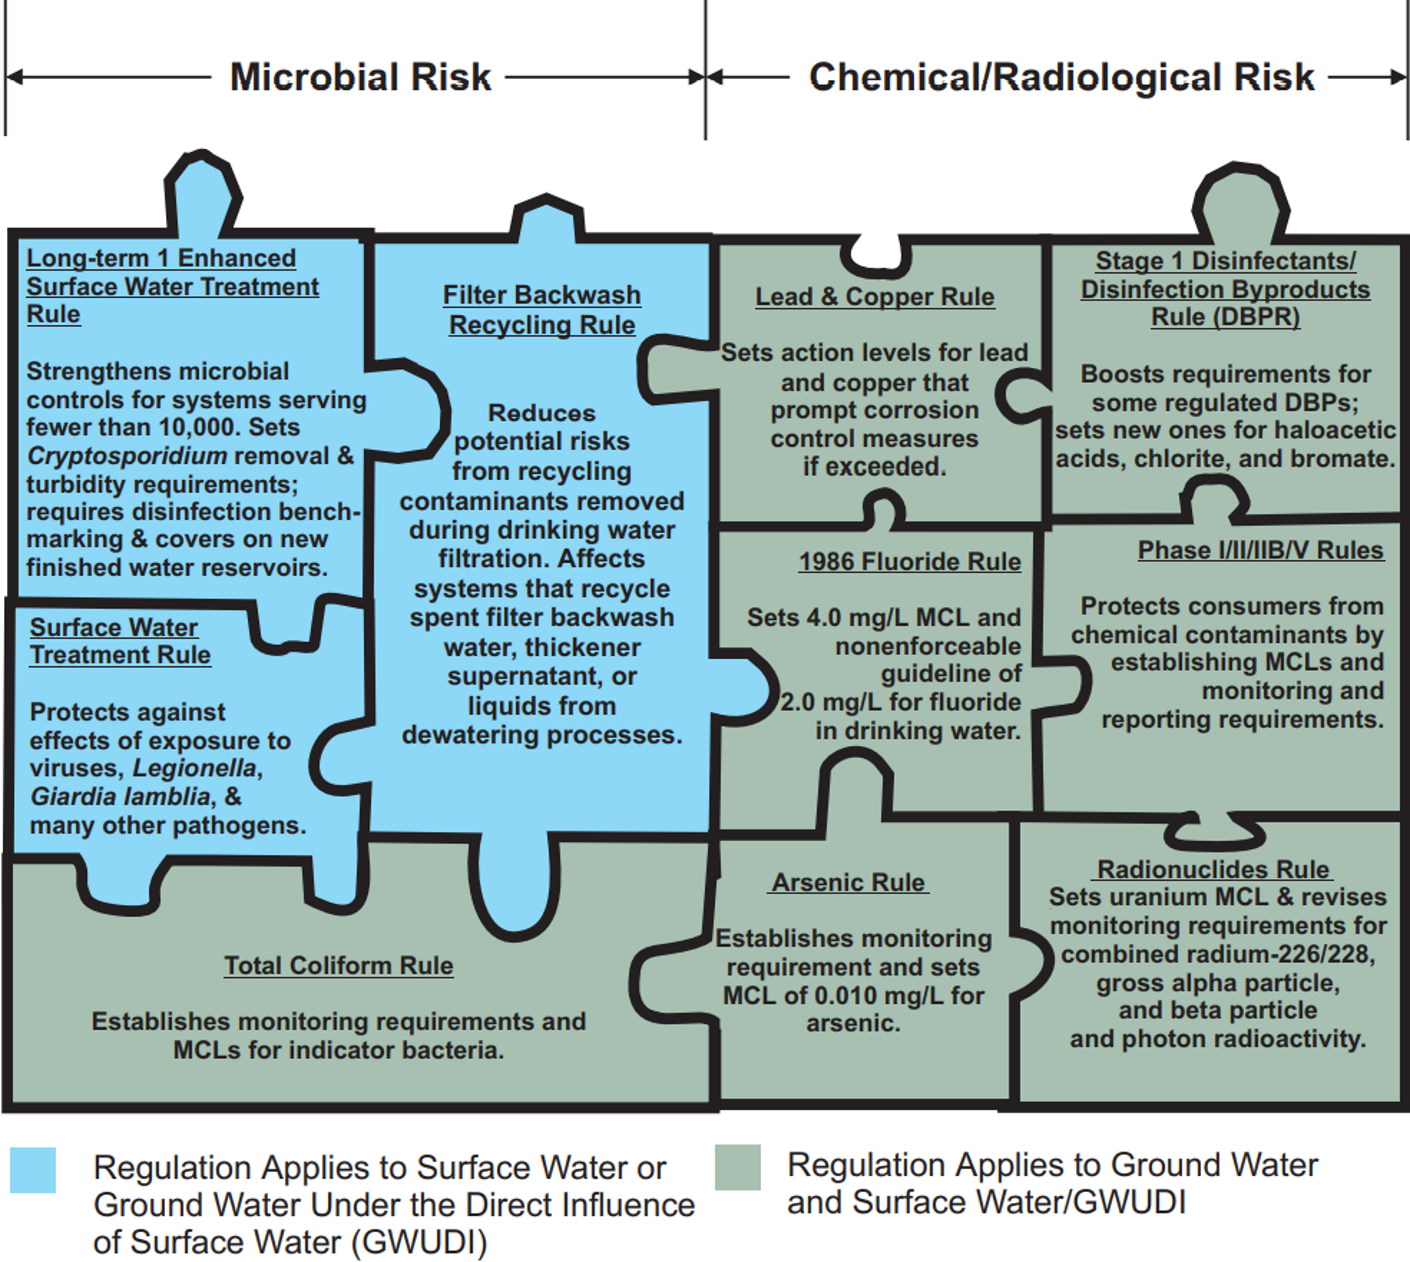
\includegraphics[scale=0.35]{WaterRegulations}
\caption{Summary of water regulations}
\end{center}
\end{figure}

\subsection{Surface Water Treatment Rule}\index{Surface water treatment rule (SWTR)}
\begin{itemize}
\item Adopts a "Multiple Barriers" approach which relies on:
\begin{itemize}
\item \textbf{Pathogen removal} Requires systems to filter unless specific avoidance criteria is met \index{Surface water treatment rule (SWTR)!Pathogen removal}.  
\item \textbf{Pathogen inactivation} \index{Surface water treatment rule (SWTR)!Pathogen inactivation} Requires all systems to disinfect.
\end{itemize}
\item Awards "Credits" for both above. 
\item Requires most water systems to filter and disinfect water from surface water sources or GWUDISW
\item Establishes maximum contaminant level goals (\textbf{MCLGs}) for viruses, bacteria and \textit{Giardia lamblia}
\item Included treatment technique (TT) requirements for filtered and unfiltered systems to protect against adverse health effects of exposure to pathogens


\end{itemize}

\subsection{Interim Enhanced Surface Water Treatment Rule}\index{Interim enhanced surface water treatment rule (IESWTR)}
\begin{itemize}
\item The 1998 Interim Enhanced Surface Water Treatment Rule (\textbf{IESWTR}) increased the level of protection from exposure to Cryptosporidium and other pathogens in drinking water supplies through improvements in filtration at water systems, provided under the original SWTR.
\item IESWTR applies to all public water systems using surface water, or GWUDISW, that serve 10,000 or more persons
\item The SWTR and the Interim ESWTR includes the following general requirements in order to minimize human exposure to microbial contaminants in drinking water:
\end{itemize}

\subsection{Long-Term 1 Enhanced Surface Water Treatment Rule}\index{Long-term 1 enhanced surface water treatment rule (LT1ESWTR)}
\begin{itemize}
\item The Long-Term 1 Enhanced Surface Water Treatment Rule (\textbf{LT1ESWTR}) applies to all public water systems using surface water, or GWUDISW, serving fewer than 10,000  persons
\item The LT1ESWTR builds upon the framework established for systems serving a population of 10,000 or more in the Interim Enhanced Surface Water Treatment Rule (IESWTR). 
\item While there are small differences between the LT1ESWTR and IESWTR, these differences reflect an effort to reduce burden for small systems while still maintaining a comparable level of health protection.
\end{itemize}


\subsection{Long-Term 2 Enhanced Surface Water Treatment Rule}\index{Long-term 2 enhanced surface water treatment rule (LT2ESWTR)}
\begin{itemize}
\item The Long-Term 2 Enhanced Surface Water Treatment Rule (\textbf{LT2ESWTR}) applies to all PWSs that use surface water or GWUDISW
\item Targets additional Cryptosporidium treatment requirements to higher risk systems
\item Requires provisions to reduce risks from uncovered finished water storage facilities
\item Provides provisions to ensure that systems maintain microbial protection as they take steps to reduce the formation of disinfection byproducts
\end{itemize}

\subsection{Requirements under Surface Water Treatment Rules} \index{Surface water treatment rule (SWTR)!Requirements}
\begin{itemize}
\item Utilities are required to achieve at least:
\begin{itemize}
\item 99.9\% removal and/or inactivation of Giardia lamblia cysts (3-log removal)
\item Minimum 99.99\% removal and/or inactivation of viruses (4-log removal)
\item A 2-log removal of Cryptosporidium. 
\end{itemize}

\item Control of Cryptosporidium \index{Control of cyrptosporidium}:
\begin{itemize}
\item The maximum contaminant level goal (MCLG) is set at zero.
\item Filtered systems must physically remove 99\% (2-log) of Cryptosporidium.
\item  Unfiltered systems must update their watershed control programs to  minimize the potential for contamination by Cryptosporidium oocysts
\end{itemize}
\item Removal credit:
\vspace{0.3cm}
\begin{itemize}
\item The level of removal credit given a utility for both Giardia lamblia and viruses is determined by the type of treatment process used. 
\item For a conventional water treatment plant the SWTR provides a 2.5-log removal credit for Giardia lamblia and a 2.0-log removal credit for viruses. 
\item water treatment plants meeting the turbidity performance standard of 0.3 NTU in 95\% of the monthly measurements also get credit for a 2-log reduction in Cryptosporidium.
\end{itemize}
\vspace{0.3cm}
\item Disinfection credit:
\vspace{0.3cm}
\begin{itemize}
\item Disinfection during conventional treatment (assuming all operational criteria and performance standards are met), must achieve 0.5-log inactivation of Giardia lamblia and 2.0-log inactivation of viruses. 
\item As a substitute to actually measuring the inactivation of Giardia lamblia and viruses achieved at a treatment plant, the SWTR established the concept of CT to evaluate inactivation. CT is the product of the concentration of disinfectant remaining at the end of a treatment process (“C” in milligrams per liter) and the contact time in which 10\% of the water passes through the treatment process (“T” or “T10” in minutes). The SWTR provides tables which identify the log removal of both Giardia lamblia and viruses achieved for a calculated CT value based on the type of disinfectant, the water temperature, and pH.
\end{itemize}
\item Turbidity monitoring requirements include:
\begin{itemize}
\item For treatment plants using conventional treatment or direct filtration, a turbidity performance standard for the combined filter effluent (CFE) \index{Combined filter effluent (CFE)} of 1 NTU as a maximum, and 0.3 NTU as a maximum in 95 percent of monthly measurements, based on 4-hour monitoring.
\item Continuous monitoring of individual filter effluent (IFE) \index{Individual filter effluent (IFE)} turbidity in conventional and direct filtration plants and recording of IFE turbidity readings every 15 minutes.
\end{itemize}
\item Reporting and recordkeeping requirements include \index{Surface water treatment rule (SWTR)!Reporting and recordkeeping}:
\begin{itemize}
\item PWSs must report turbidity measurements related to CFE monitoring to the state within 10 days after the end of each month the PWS serves water to the public.

\item PWSs must keep CFE turbidity monitoring records and any other turbidity analyses, with the exception of IFE monitoring records, for at least 5 years. 

\item PWSs must keep records from IFE turbidity monitoring for at least 3 years.
\end{itemize}
\item If a system meets the turbidity performance standard of 0.3 NTU in 95\% of the samples taken each month (never to exceed 1 NTU) than the system gets credit for achieving the 2-log reduction in Cryptosporidium.

\item PWSs using alternative filtration techniques [defined as filtration other than conventional, direct, slow sand, or diatomaceous earth (DE)] must demonstrate to the state the ability to consistently achieve 2-log removal of Cryptosporidium and comply with specific state-established CFE turbidity requirements.


\item The required level of removal/inactivation must occur between the point where the raw water is not longer subject to surface water runoff and the point at which the first customer is served.

\item The disinfectant residual entering the distribution system must not fall below 0.2 mg/L for more than 4 hr during any 24- hr period.

\item A disinfectant residual must be detectable in 95\% of distribution system samples. A heterotrophic plate count (HPC) \index{Heterotrophic plate count} concentration of less than 500 colonies per milliliter can serve as a detectable residual if no residual is measured.

\item Each utility must perform a watershed sanitary survey at least every 5 years.

\end{itemize}
\begin{figure}[H]
\begin{center}
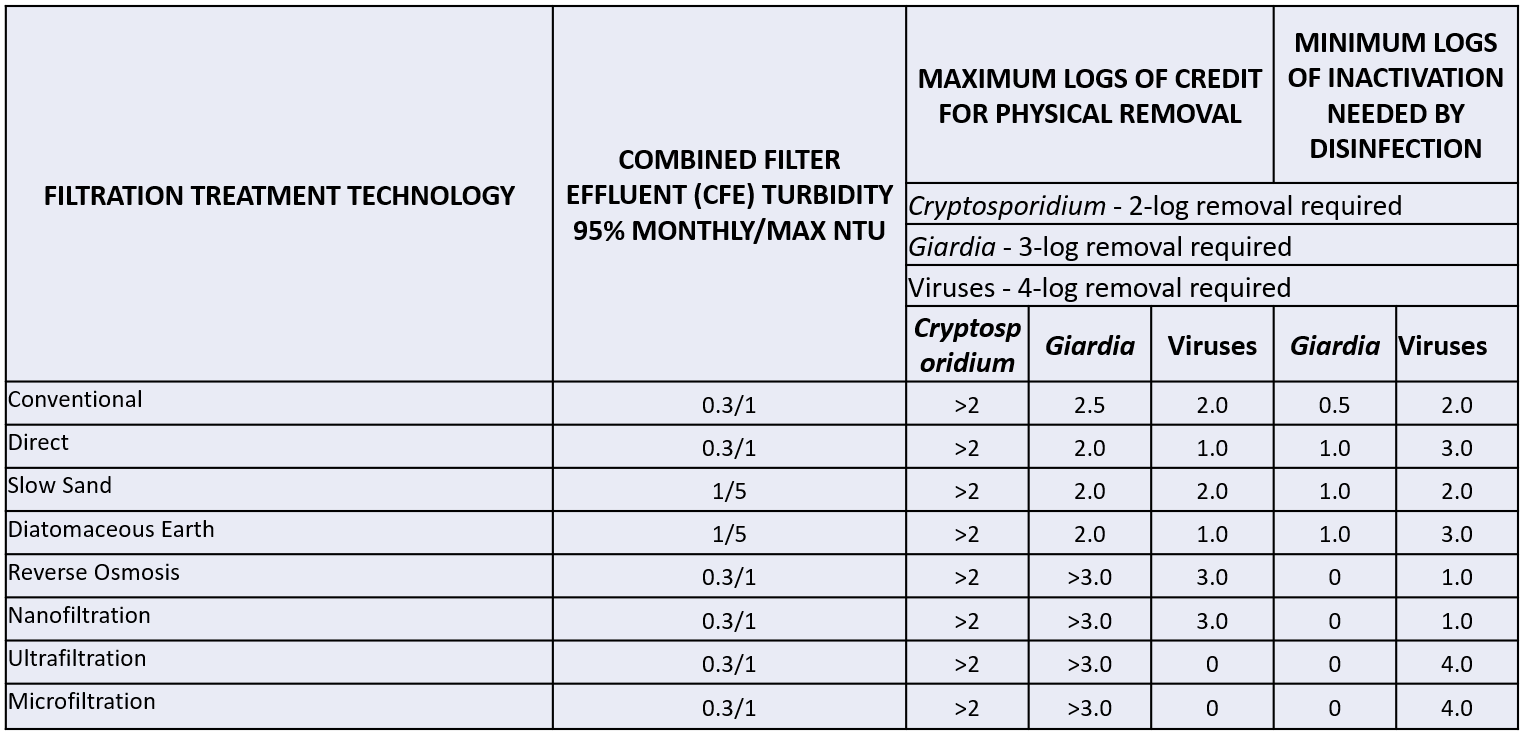
\includegraphics[scale=0.35]{SWTRAutoRemovalCredits}
\caption{SWTR auto removal credits}
\end{center}
\end{figure}


\nopagebreak


\newpage
\thispagestyle{empty}
\begin{landscape}
\begin{table}[h!]
  \centering
\small
\begin{tabular}{|lllll|}
\hline
\rowcolor[HTML]{CBCEFB} 
\multicolumn{2}{|l|}{\cellcolor[HTML]{CBCEFB}TCR/ Nitrate/Nitrite}                                                   & \multicolumn{1}{l|}{\cellcolor[HTML]{CBCEFB}CWS} & \multicolumn{1}{l|}{\cellcolor[HTML]{CBCEFB}NTNCWS} & TNCWS                      \\ \hline
\multicolumn{2}{|l|}{Sanitary Survey}                                                                                & \multicolumn{1}{l|}{Every 3 years}               & \multicolumn{1}{l|}{Every 5 years}                  & Every 5 years              \\ \hline
\multicolumn{2}{|l|}{Total Coliform Bacteria1}                                                                       & \multicolumn{1}{l|}{Monthly}                     & \multicolumn{1}{l|}{Monthly}                        & Monthly                    \\ \hline
\multicolumn{2}{|l|}{Nitrate (NO$_3$)}                                                                                  & \multicolumn{1}{l|}{Quarterly$^2$}                  & \multicolumn{1}{l|}{Quarterly$^2$}                     & Annually                   \\ \hline
\multicolumn{2}{|l|}{Nitrite (NO$_2$)}                                                                                  & \multicolumn{1}{l|}{1 sample record}             & \multicolumn{1}{l|}{1 sample record}                & 1 sample record            \\ \hline
\rowcolor[HTML]{CBCEFB} 
\multicolumn{2}{|l|}{\cellcolor[HTML]{CBCEFB}Reporting}                                                              & \multicolumn{1}{l|}{\cellcolor[HTML]{CBCEFB}CWS} & \multicolumn{1}{l|}{\cellcolor[HTML]{CBCEFB}NTNCWS} & TNCWS                      \\ \hline
\multicolumn{2}{|l|}{}                                                                                               & \multicolumn{1}{l|}{Continuous or grab samples}  & \multicolumn{1}{l|}{Continuous or grab samples}     & Continuous or grab samples \\ \hline
\multicolumn{2}{|l|}{Turbidity}                                                                                      & \multicolumn{3}{l|}{(Frequency determined by population and   filtration type.)}                                                    \\ \hline
\multicolumn{2}{|l|}{Fluoride – if added}                                                                            & \multicolumn{1}{l|}{Daily}                       & \multicolumn{1}{l|}{Daily}                          &                            \\ \hline
\multicolumn{2}{|l|}{}                                                                                               & \multicolumn{1}{l|}{Continuous or grab samples}  & \multicolumn{1}{l|}{Continuous or grab samples}     & Continuous or grab samples \\ \cline{3-5} 
\multicolumn{2}{|l|}{\multirow{-2}{*}{Entry Point Chlorine – if chlorine is added}}                                  & \multicolumn{3}{l|}{(Pop determines how many times a   day chlorine is measured.)}                                                  \\ \hline
\multicolumn{2}{|l|}{Distribution System Chlorine3}                                                                  & \multicolumn{1}{l|}{Monthly}                     & \multicolumn{1}{l|}{Monthly}                        & Monthly                    \\ \hline
\multicolumn{2}{|l|}{Consumer Confidence Report}                                                                     & \multicolumn{1}{l|}{Annually}                    & \multicolumn{1}{l|}{Annually}                       &                            \\ \hline
\rowcolor[HTML]{CBCEFB} 
\multicolumn{2}{|l|}{\cellcolor[HTML]{CBCEFB}Disinfection/Disinfectant Byproducts}                                   & \multicolumn{1}{|l|}{\cellcolor[HTML]{CBCEFB}CWS} & \multicolumn{1}{|l|}{\cellcolor[HTML]{CBCEFB}NTNCWS} & TNCWS                      \\ \hline
\multicolumn{1}{|l|}{}                                                      & \multicolumn{1}{l|}{Pop \textless 500} & \multicolumn{1}{l|}{Annually}                    & \multicolumn{1}{l|}{Annually}                       & Annually                   \\ \cline{2-5} 
\multicolumn{1}{|l|}{}                                                      & \multicolumn{1}{l|}{Pop 500 -   9,999} & \multicolumn{1}{l|}{Quarterly}                   & \multicolumn{1}{l|}{Quarterly}                      & Quarterly                  \\ \cline{2-5} 
\multicolumn{1}{|l|}{\multirow{-3}{*}{Total   Trihalomethanes (TTHM/HAA5)}} & \multicolumn{1}{l|}{Pop 10,000}        & \multicolumn{1}{l|}{Quarterly}                   & \multicolumn{1}{l|}{Quarterly}                      & Quarterly                  \\ \hline
\multicolumn{2}{|l|}{TOC and Alkalinity}                                                                             & \multicolumn{1}{l|}{Monthly2}                    & \multicolumn{1}{l|}{Monthly2}                       &                            \\ \hline
\multicolumn{2}{|l|}{Bromate (Ozone plants only)}                                                                    & \multicolumn{1}{l|}{Monthly}                     & \multicolumn{1}{l|}{Monthly}                        &                            \\ \hline
\rowcolor[HTML]{CBCEFB} 
\multicolumn{2}{|l|}{\cellcolor[HTML]{CBCEFB}Inorganic Chemicals}                                                    & \multicolumn{1}{l|}{\cellcolor[HTML]{CBCEFB}CWS} & \multicolumn{1}{l|}{\cellcolor[HTML]{CBCEFB}NTNCWS} & TNCWS                      \\ \hline
\multicolumn{2}{|l|}{All Primary}                                                                                    & \multicolumn{1}{l|}{Annually}                    & \multicolumn{1}{l|}{Annually}                       &                            \\ \hline
\multicolumn{2}{|l|}{Arsenic}                                                                                        & \multicolumn{1}{l|}{Annually}                    & \multicolumn{1}{l|}{Annually}                       &                            \\ \hline
\multicolumn{2}{|l|}{Asbestos}                                                                                       & \multicolumn{1}{l|}{Once per period}             & \multicolumn{1}{l|}{Once per period}                &                            \\ \hline
\multicolumn{2}{|l|}{Lead and Copper1}                                                                               & \multicolumn{1}{l|}{Every 6 months$^2$}             & \multicolumn{1}{l|}{Every 6 months$^2$}                &                            \\ \hline
\rowcolor[HTML]{CBCEFB} 
\multicolumn{2}{|l|}{\cellcolor[HTML]{CBCEFB}Organic Chemicals}                                                      & \multicolumn{1}{l|}{\cellcolor[HTML]{CBCEFB}CWS} & \multicolumn{1}{l|}{\cellcolor[HTML]{CBCEFB}NTNCWS} & TNCWS                      \\ \hline
\multicolumn{2}{|l|}{Pesticides (SOCs) and Other Organics}                                                           & \multicolumn{1}{l|}{Quarterly$^2$}                  & \multicolumn{1}{l|}{Quarterly$^2$}                     &                            \\ \hline
\multicolumn{2}{|l|}{}                                                                                               & \multicolumn{1}{l|}{Quarterly}                   & \multicolumn{1}{l|}{Quarterly}                      &                            \\ \cline{3-5} 
\multicolumn{2}{|l|}{\multirow{-2}{*}{Volatile Organic Chemicals (VOCs)}}                                            & \multicolumn{1}{l|}{Annually}                    & \multicolumn{1}{l|}{Annually}                       &                            \\ \hline
\rowcolor[HTML]{CBCEFB} 
\multicolumn{2}{|l|}{\cellcolor[HTML]{CBCEFB}Radionuclides}                                                          & \multicolumn{1}{l|}{\cellcolor[HTML]{CBCEFB}CWS} & \multicolumn{1}{l|}{\cellcolor[HTML]{CBCEFB}NTNCWS} & TNCWS                      \\ \hline
\multicolumn{2}{|l|}{Gross Alpha Radioactivity}                                                                      & \multicolumn{1}{l|}{Quarterly}                   & \multicolumn{1}{l|}{}                               &                            \\ \hline
\multicolumn{2}{|l|}{Radium 226, Radium 228, Uranium}                                                                & \multicolumn{1}{l|}{Quarterly}                   & \multicolumn{1}{l|}{}                               &                            \\ \hline

\multicolumn{5}{|l|}{\begin{tabular}[c]{@{}l@{}}$^1$ Number of samples is based on   population.\\     $^2$   May be   reduced if certain criteria are met.\\      $^3$   Distribution point chlorine   test is required at the same time and location as total coliform samples are   collected\\Cycle - 3 years\\ Period – 9 years\end{tabular}}

\\ \hline
\end{tabular}
%
%
%
%
%
%
%
%
%
%\multicolumn{5}{|l|}{1 Number of samples is based   on population. 2 May be   reduced if certain criteria are met.}                                                                                                                                        \\ \hline
%\multicolumn{5}{|l|}{3 Distribution point chlorine   test is required at the same time and location as total coliform samples are   collected.}                                                                                                            \\ \hline
%\multicolumn{5}{|l|}{Cycle – 3 years; Period – 9 years}                                                                                                                                                                                                    \\ \hline
%\end{tabular}
\caption{Sampling and testing schedules for surface water and GUDISW}
%\textit{(Source:Introduction to Small Water Systems - Alaska DEC)}

\end{table}
\end{landscape}

\section{Total Coliform Rule}\index{Total coliform rule (TCR)}
\begin{itemize}
\item The 1989 Total Coliform Rule (\textbf{TCR})promotes surveillance of distribution system water quality targeting fecal matter and/or pathogens.
\item Rule requires collection of monthly samples that are representative of water throughout the distribution system as identified in its approved Sample Siting Plan.
\item For systems serving >1,000 people, number of monthly samples that need to be collected is based upon the population served.  
\item The presence of total coliforms is a warning sign that the system is vulnerable to contamination. It does not necessarily mean that the system is contaminated.
\item If sample is total coliform (TC) positive:
\begin{enumerate}[A.]
\item Conduct follow up testing:
\begin{enumerate}[1.]
\item In the same sample, determine fecal coliform (FC) or E. Coli (EC).
\item Collect a second sample within 24 hours, and reanaylze TC and FC/EC. 
\end{enumerate}
\item The system is not in compliance if:
\begin{enumerate}[i.]
\item The analysis and reanalysis of a given sampling location are TC positive (TC[+]) both times and FC[/EC+] at least one of these times. \textbf{OR}
\item More than 5 percent of all monthly samples for a 12-month period are TC[+].
\end{enumerate}
\end{enumerate}

\end{itemize}

\begin{figure}[]
\begin{center}
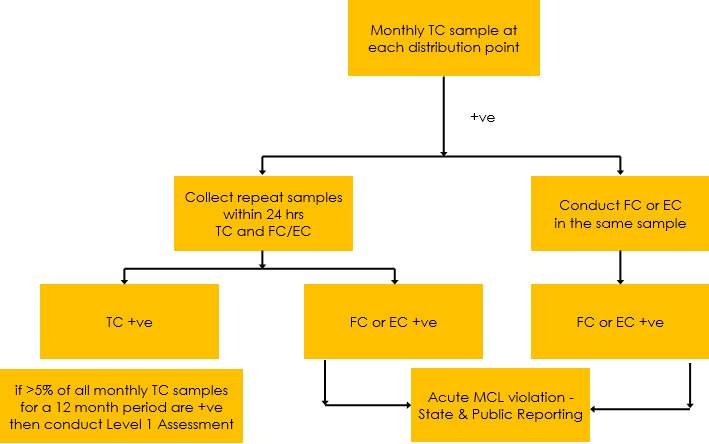
\includegraphics[scale=0.65]{TCRSummary}
\caption{Summary of Total Coliform Rule requirements}
\end{center}
\end{figure}




\subsection{Revised Total Coliform Rule}\index{Revised total coliform rule (RTCR)}
\begin{itemize}
\item The 2013 Revised Total Coliform Rule (\textbf{rTCR})revises the 1989 Total Coliform Rule (\textbf{TCR}) and is applicable to all PSWs. 
\item Establishes a \textbf{zero} MCL and MCLG for EC and eliminated MCLG and MCL for TC.  EC being a more specific indicator of fecal contamination and potentially harmful pathogens than
TC and also many of the organisms detected by total coliform methods are not of fecal origin and do not have any direct public health implication. 
\item The revised rule changes total coliform detection from a MCL to a Treatment Technique
Trigger, requiring the PWS to perform a system review and fix any potential breaches in
the microbiological barriers. Detection of E. coli during sampling indicates the
exceedance of the MCL. These detections also trigger an inspection and correction of any
sanitary defects found. The rTCR also increases monitoring for many systems experiencing compliance issues or that do not have a microbiologically protected source.
\item Requirements for monitoring TC and EC according to a sample siting plan and schedule specific to the PWS.
\item Requires sampling site representative of the entire distribution system.
\item Eliminated TCR's public notification requirements based only on the presence of TC and instead requires public notification when:
\begin{enumerate}
\item When an an EC MCL violation occurs \textbf{OR}
\item When a PWS fails to conduct the required assessment and corrective action.
\end{enumerate}
\item Uses vulnerable PWS to initiate a "find and fix" approach to address fecal contamination that could enter the distribution system.
\item rTCR requires PWS to perform assessments to identify sanitary defects - that could provide a pathway of entry for microbial contamination, or those that indicate failure (existing or potential) of protective barriers against microbial contamination, and subsequently take action to correct them.
\item There are two levels of assessments based on the severity or frequency of the problem:
\begin{enumerate}
\item A Level 1 assessment is required if:
\begin{itemize}
\item For systems taking 40 or more samples per month, the utility exceeds 5.0 percent total coliform-positive samples for the month; or
\item For systems taking fewer than 40 samples per month, the utility has two or more total coliform-positive samples in the same month; or
\item The Utility fails to take every required repeat sample after any single routine total coliform-positive sample.
\end{itemize}

\item Level 2 which is an in-depth examination of the distribution system, water sources, treatment facilities, storage facilities and relevant operational practices at a public water system (PWS) conducted by an assessor - state or state-approved entity. Level 2 assessment is triggered by an E.Coli MCL violation or a second Level 1 assessment in a 12-month period or in two consecutive years.
\item When sanitary defects are identified during a Level 1 or Level 2 Assessment, they should be corrected as soon as possible to protect public health.
\end{enumerate}

\item A public water system will receive a Treatment Technique violation when any of the following occur:
\begin{itemize}
\item Failure to conduct a Level 1 or Level 2 Assessment within 30 days of a trigger.
\item Failure to correct all sanitary defects from a Level 1 or Level 2 Assessment within
30 days of a trigger or in accordance with the state-approved time frame.
\item Failure of a seasonal system to complete state-approved start-up procedures prior to serving water to the public.
\end{itemize}
\end{itemize}

\subsection{Filter Backwash Recycle Rule}\index{Filter backwash recycle rule}
\begin{itemize}
\item Filter Backwash Recycle Rule (\textbf{FBRR})applies to all public water systems using conventional or direct filtration to treat surface water, or GWUDISW, regardless of size
\item Requires PWSs to review their backwash water recycling practices to ensure that they do not compromise microbial control
\item Requires recycled filter backwash water to go through all processes of a system’s conventional or direct filtration treatment. 
\end{itemize}

\section{Groundwater rules}\index{Groundwater rules}
\begin{itemize}
\item The Federal Groundwater Rules (\textbf{GWR}) rule applies to public water systems that use groundwater as a source of drinking water.
\item Goal of the GWR is increased protection against microbial pathogens. 
\item groundwater systems that are at risk of fecal contamination must take corrective action. Corrective action reduces potential illness from exposure to microbial pathogens. The 
\item The GWR relies on four major components:
\begin{enumerate}
\item Routine sanitary surveys of systems that require the evaluation of critical elements of a public water system and the identification of significant deficiencies (e.g., a well located near a leaking septic system);
\item Triggered source water monitoring for a system that (not treating drinking water to remove 99.99 percent (4-log) of viruses) identifies a positive sample during regular Total Coliform monitoring or assessment monitoring (at the option of the state) targeted at high-risk systems
\item Corrective action is required for any system with a significant deficiency or source water fecal contamination; and
\item Compliance monitoring to ensure that treatment technology installed to treat drinking water reliably achieves 99.99 percent (4-log) inactivation or removal of viruses.
\end{enumerate}
\item In California, the Sustainable Groundwater Management Act (\textbf{SGMA})sets a timeline to identify responsible local agencies – which will work as a team – the means to reverse overdrafted conditions in certain areas and to ensure the 127 “high and medium priority” groundwater basins or sub-basins not in overdraft reach sustainability by 2040.
\end{itemize}

\newpage
\thispagestyle{empty}
\begin{landscape}
\begin{table}[h!]
  \centering
\small
\begin{tabular}{|l|l|l|l|l|}
\hline
\rowcolor[HTML]{CBCEFB} 
\multicolumn{2}{|l|}{\cellcolor[HTML]{CBCEFB}\textbf{TCR/ Nitrate/Nitrite}}                                             & \multicolumn{1}{l|}{\cellcolor[HTML]{CBCEFB}\textbf{CWS}}             & \multicolumn{1}{l|}{\cellcolor[HTML]{CBCEFB}\textbf{NTNCWS}}             & \multicolumn{1}{l|}{\cellcolor[HTML]{CBCEFB}\textbf{TNCWS}}             \\ \hline
\multicolumn{2}{|l|}{Sanitary Survey}                                                                                   & Every 5 years                                                        & Every 5 years                                                           & Every 5 years                                                          \\
\multicolumn{2}{|l|}{Total Coliform Bacteria$^1$}                                                                          & Every month                                                          & Every month                                                             & Every quarter                                                          \\
\multicolumn{2}{|l|}{Nitrate (NO3)}                                                                                     & Annually                                                             & Annually                                                                & Annually                                                               \\
\multicolumn{2}{|l|}{Nitrite (NO2)}                                                                                     & 1 sample record                                                      & 1 sample record                                                         & 1 sample record                                                        \\ \hline
\rowcolor[HTML]{CBCEFB} 
\multicolumn{2}{|l|}{\cellcolor[HTML]{CBCEFB}\textbf{Reporting}}                                                        & \multicolumn{1}{l|}{\cellcolor[HTML]{CBCEFB}\textbf{CWS}}             & \multicolumn{1}{l|}{\cellcolor[HTML]{CBCEFB}\textbf{NTNCWS}}             & \multicolumn{1}{l|}{\cellcolor[HTML]{CBCEFB}\textbf{TNCWS}}             \\ \hline
\multicolumn{2}{|l|}{Fluoride – if added}                                                                               & Daily                                                                & Daily                                                                   & Daily                                                                  \\
\multicolumn{2}{|l|}{}                                                                                                  & Continuous or grab samples                                           & Continuous or grab samples                                              & Continuous or grab samples                                             \\
\multicolumn{2}{|l|}{\multirow{-2}{*}{Entry Point Chlorine – if chlorine is added}}                                 & \multicolumn{3}{|l|}{(Pop determines how many times   a day chlorine is measured.)}                                                                                                                                       \\
\multicolumn{2}{|l|}{Distribution Chlorine$^2$ – if chlorine is added}                                                   & Monthly                                                              & Monthly                                                                 &                                                                        \\
\multicolumn{2}{|l|}{Consumer Confidence Report}                                                                        & Annually                                                             &                                                                         &                                                                        \\ \hline
\rowcolor[HTML]{CBCEFB} 
\multicolumn{2}{|l|}{\cellcolor[HTML]{CBCEFB}\textbf{Disinfection/Disinfectant Byproducts}}                         & \multicolumn{1}{l|}{\cellcolor[HTML]{CBCEFB}\textbf{CWS}}             & \multicolumn{1}{l|}{\cellcolor[HTML]{CBCEFB}\textbf{NTNCWS}}             & \multicolumn{1}{l|}{\cellcolor[HTML]{CBCEFB}\textbf{TNCWS}}             \\
                                                                         & Pop \textless 500 – 9,999                  & Annually                                                             & Annually                                                                &                                                                        \\
\multirow{-2}{*}{Total Trihalomethanes$^1$ (TTHM/HAA5)}                   & Pop $\geq$ 10,000                                & Quarterly                                                            & Quarterly                                                               &                                                                        \\ \hline
\multicolumn{2}{|l|}{Bromate (Ozone plants only)}                                                                       & Monthly                                                              & Monthly                                                                 &                                                                        \\ \hline
\rowcolor[HTML]{CBCEFB} 
\multicolumn{2}{|l|}{\cellcolor[HTML]{CBCEFB}Inorganic Chemicals}                                                       & \multicolumn{1}{l|}{\cellcolor[HTML]{CBCEFB}CWS}                      & \multicolumn{1}{l|}{\cellcolor[HTML]{CBCEFB}NTNCWS}                      & \multicolumn{1}{l|}{\cellcolor[HTML]{CBCEFB}TNCWS}                      \\ \hline
\multicolumn{2}{|l|}{All Primary}                                                                                       & Once per period                                                      & Once per period                                                         &                                                                        \\
\multicolumn{2}{|l|}{Arsenic}                                                                                           & Once per period                                                      & Once per period                                                         &                                                                        \\
\multicolumn{2}{|l|}{Asbestos}                                                                                          & Once per cycle                                                       & Once per cycle                                                          &                                                                        \\
\multicolumn{2}{|l|}{Lead and Copper$^1$}                                                                                  & Every 6 months$^3$                                                      & Every 6 months$^3                                                        $ &                                                                        \\ \hline
\rowcolor[HTML]{CBCEFB} 
\multicolumn{2}{|l|}{\cellcolor[HTML]{CBCEFB}\textbf{Organic Chemicals}}                                                & \multicolumn{1}{l|}{\cellcolor[HTML]{CBCEFB}\textbf{CWS}}             & \multicolumn{1}{l|}{\cellcolor[HTML]{CBCEFB}\textbf{NTNCWS}}             & \multicolumn{1}{l|}{\cellcolor[HTML]{CBCEFB}\textbf{TNCWS}}             \\ \hline
\multicolumn{2}{|l|}{Pesticides (SOCs) and Other   Organics}                                                            & Every quarter3                                                       & Every quarter3                                                          &                                                                        \\
\multicolumn{2}{|l|}{}                                                                                                  & Every quarter                                                        & Every quarter                                                           &                                                                        \\
\multicolumn{2}{|l|}{\multirow{-2}{*}{Volatile Organic Chemicals   (VOCs)}}                                             & Annually                                                             & Annually                                                                &                                                                        \\ \hline
\rowcolor[HTML]{CBCEFB} 
\multicolumn{2}{|l|}{\cellcolor[HTML]{CBCEFB}\textbf{Radionuclides}}                                                    & \multicolumn{1}{c}{\cellcolor[HTML]{CBCEFB}\textbf{CWS}}             & \multicolumn{1}{c}{\cellcolor[HTML]{CBCEFB}\textbf{NTNCWS}}             & \multicolumn{1}{c}{\cellcolor[HTML]{CBCEFB}\textbf{TNCWS}}             \\
\multicolumn{2}{|l|}{Gross Alpha Radioactivity}                                                                         & Every quarter                                                        &                                                                         &                                                                        \\
\multicolumn{2}{|l|}{Radium 226, Radium 228, Uranium}                                                                   & Every quarter                                                        &                                                                         &                                                                       
\\ \hline
\multicolumn{5}{|l|}{\begin{tabular}[c]{@{}l@{}}$^1$ Number of samples is based on   population.\\     $^2$   Distribution   point chlorine test is required at the same time and location as total   coliform samples are collected.\\      $^3$   May   be reduced if certain criteria are met.\\      Cycle – 3 years\\      Period – 9 years\end{tabular}}\\
\hline
\end{tabular}
\caption{Sampling and testing schedules for groundwater}
\end{table}
\end{landscape}

\section{Microbial and disinfection byproducts rules}\index{Microbial and disinfection byproducts rules}
\begin{itemize}
\item The Microbial and Disinfection Byproducts Rules (\textbf{MDBPs}) include Stage 1 and Stage 2 Disinfectants and Disinfection Byproducts Rules (\textbf{DBPRs}) 
\item As disinfectants can react with naturally-occurring materials in the water to form byproducts including:
\begin{itemize}
\item Trihalomethanes (THM),
\item Haloacetic acids (HAA),
\item Chlorite, and
\item Bromate.
\end{itemize}
\item The Stage 1 and Stage 2 DBPRs are intended to minimize the public
health risk from DBPs and disinfectants that are used to control pathogens.
\item Under these rules, EPA established:
\begin{itemize}
\item Maximum residual disinfectant levels (MRDLs) \index{Maximum residual disinfectant levels (MRDLs)}for chlorine, chloramines and chlorine dioxide, and
\item  MCLs for DBPs - chlorite, bromate, TTHM and HAA5.
\end{itemize}
\item These Rules apply to all Community Water Systems (\textbf{CWS}) and Non-Transient Non-Community Water Systems (\textbf{NTNCWS}) that add/deliver a primary or residual disinfectant, and TNCWs that use chlorine dioxide. 
\item This Rule does not apply to water systems that use ultraviolet (UV) light.
\item The maximum residual disinfectant levels (\textbf{MRDLs}), and maximum residual disinfectant level goals (\textbf{MRDLGs}) for the three chemical disinfectants are listed in Table \ref{table:DisinfectantMRDLs} \index{Disinfectant MRDLs}.
\item The MCLs for DBPs are listed in Table \ref{table:DBPMCL}.
\begin{table}[]
\begin{center}
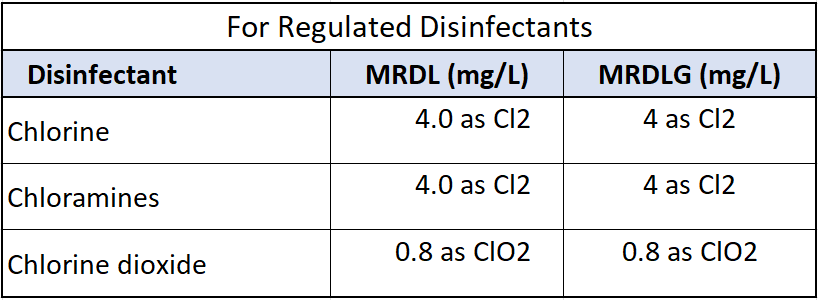
\includegraphics[scale=0.5]{DinfectantMRDLS}
\caption{Disinfectant MRDLs}
\label{table:DisinfectantMRDLs}
\end{center}
\end{table}
\begin{table}[]
\begin{center}
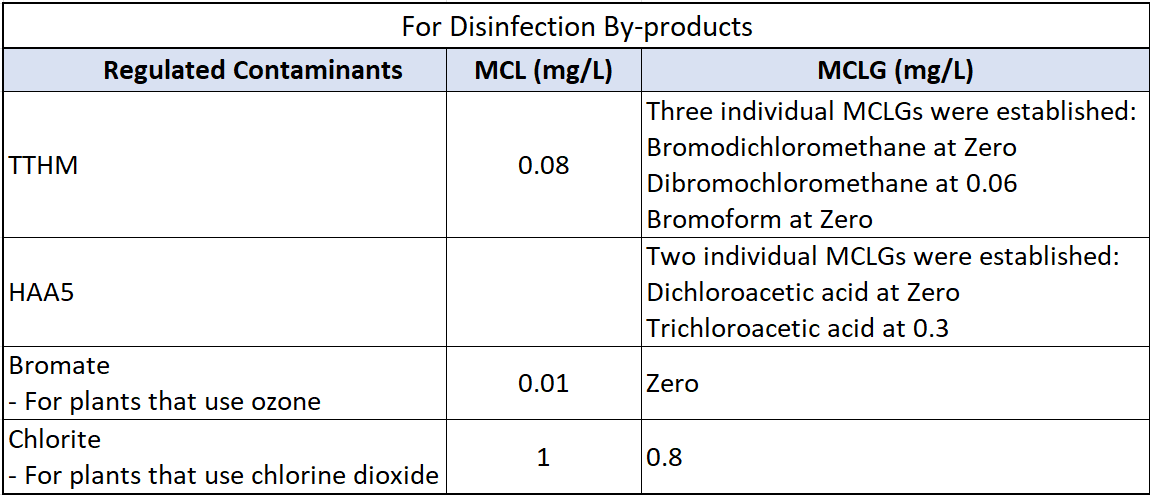
\includegraphics[scale=0.5]{DBPMCLS}
\caption{Disinfectant by-products MCLs}
\label{table:DBPMCL}
\end{center}
\end{table}
\item Compliance is based on a running annual average (RAA) calculated quarterly, locational running annual average (LRAA) calculated quarterly, a single sample result or an average of a selected number of samples, depending on which disinfectant or DBP is being monitored.
\item If the creation of these by-products causes the system to exceed the MCL for Total TTHMs (0.1 mg/l or 100 ppb), the system will be required to change to a different means of disinfection. 
\item Total chlorine residuals are also limited to a maximum of 4.0 mg/l. 
\item The D-DBP rule currently only applies to systems serving a population over 10,000.
\end{itemize}
\section{Other drinking water rules}
\subsection{Lead and Copper Rule}\index{Lead and copper rule}
\begin{itemize}
\item The objective of the 1991 Lead and Copper Rule (\textbf{LCR}) is to control corrosiveness of the finished water in drinking water distribution systems to limit the amount of lead (Pb) and copper (Cu) that may be leached from certain metal pipes and fittings in the distribution system.
\item Applies to all community water systems (CWSs) and non-transient non-community water systems (NTNCWSs)that use groundwater as a source of drinking water.
\item Establishes action level (AL) of 0.015 mg/L for Pb and 1.3 mg/L for Cu based on 90th percentile level of tap water samples.  The rule also establishes an MCLG of \textbf{zero} for lead.
\item The lead action level is a measure of the effectiveness of the corrosion control treatment
in water systems. The action level is not a standard for establishing a safe level of lead in a
home. 
\item Number of samples is based on system size - population served and Systems must conduct monitoring every 6 months unless they qualify for reduced monitoring. 
\item Utilities are required to identify sampling locations and determining initial tap water Pb and Cu levels and also monitor other water quality parameters (WQPs) at these locations to monitor and evaluate the corrosion control characteristics of supplied water.
\item Each utility must complete a survey and evaluate materials that comprise their distribution system, in addition to using other available information, to target homes that are at high risk for Pb/Cu contamination.
\item An AL exceedance is not a violation but can trigger other requirements that include water quality parameter (WQP) monitoring, corrosion control treatment (CCT), source water monitoring/treatment, public education, and lead service line replacement (LSLR).
\item Pb, Cu, and WQPs are initially collected at 6-month intervals.  This frequency can be reduced if action levels are not exceeded and optimal water treatment is maintained.
\item Systems that are in noncompliance and are performing additional corrosion-control activities must continue to monitor at six-month intervals, plus they must collect WQPs from distribution system entry points every two weeks.
\begin{table}[H]
\begin{center}
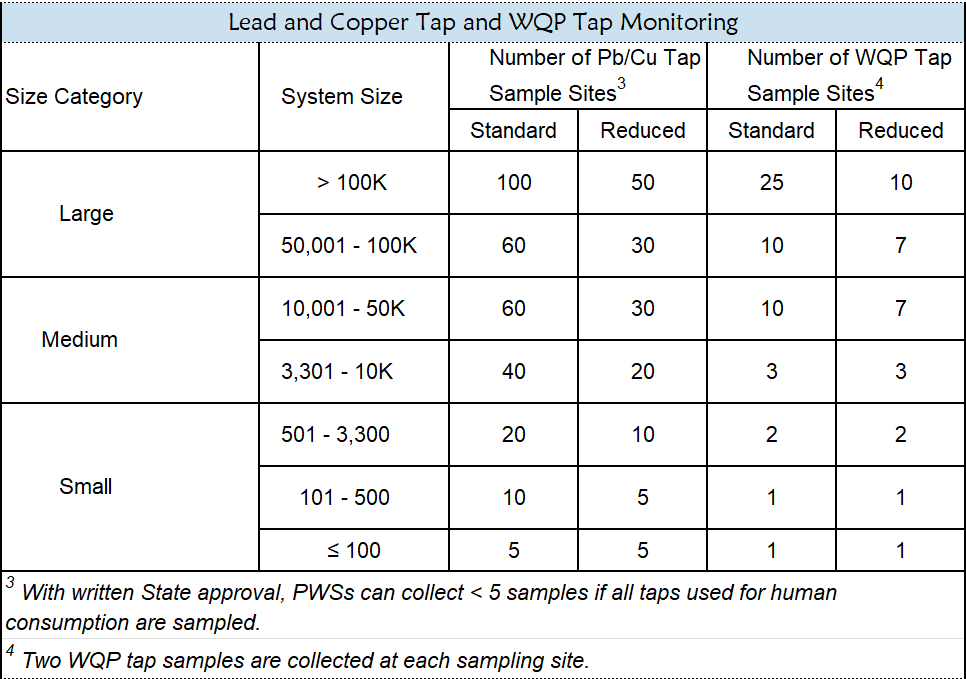
\includegraphics[scale=0.5]{LCRMonitoring}
\caption{Lead and copper tap and WQP tap monitoring}
\end{center}
\end{table}
\end{itemize}

\subsection{Radionuclides Rule}\index{Radionuclides Rule}
\begin{itemize}
\item The 2000 Radionuclide Rule regulates radionuclides in drinking water to protect public health. 
\item Radionuclides are radioactive elements which mostly enters the drinking water source from natural sources.
\item Radiation from radionuclide is known to cause cancer.
\item Radionuclide Rule applies only to Community Water Systems.
\item The rule extablishes the MCLs for radionuclides.
\newpage
\begin{figure}[H]
\begin{center}
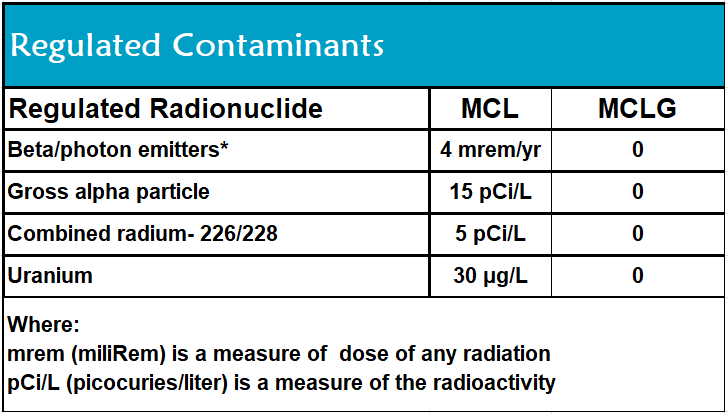
\includegraphics[scale=0.5]{RadionuclideMCL}
\caption{Radionuclide MCLs}
\end{center}
\end{figure}

\item Systems violating the MCL for one of the radionuclide, are required to work with the state to identify and implement options which may include finding a better source of water or blending.
\end{itemize}

\subsection{Arsenic Rule}\index{Arsenic Rule}
\begin{itemize}
\item Arsenic is released to the environment from a variety of natural and anthropogenic
sources. 
\begin{itemize}
\item In the environment, arsenic occurs in rocks, soil, water, air, and in biota.
\item Anthropogenic sources of arsenic relate to its use as wood preservative and in agriculture, livestock, and general industries. 
\end{itemize}
\item There is evidence that associates chronic arsenic ingestion at low concentrations with
increased risk of skin cancer, and that arsenic may cause cancers of the lung, liver, bladder,
kidney, and colon.
\item This rule establishes an Arsenic MCL of 10 ppb.

\end{itemize}
\subsection{Vulnerability assessment} \index{Vulnerability assessment}
\begin{itemize}
\item Under the Public Health Security and Bioterrorism Preparedness and Response Act of 2002,  community water systems that serve populations of greater than 3,300 persons are required to conduct vulnerability assessments.

\item Vulnerability assessments help water systems evaluate susceptibility to potential threats
and identify corrective actions that can reduce or mitigate the risk of serious consequences from
malevolent acts and natural hazards. 
. 

\item Such an assessment for a water system takes into account the vulnerability of the water supply (both ground and surface water), transmission, treatment, and distribution systems. It also considers risks posed to the surrounding community related to attacks on the water system. 

\item An effective vulnerability assessment serves as a guide to the water utility by providing a prioritized plan for security upgrades, modifications of operational procedures, and/or policy changes to mitigate the risks and vulnerabilities to the utility’s critical assets. 

\item Water systems should review their vulnerability assessments periodically to account for changing threats or additions to the system to ensure that security objectives are being met. 


\item Preferably, a vulnerability assessment is "performance-based,” meaning that it evaluates the risk to the water system based on the effectiveness (performance) of existing and planned measures to counteract adversarial actions.
\end{itemize}

\subsection{Public Notification Rule}\index{Public Notification Rule}
\begin{itemize}
\item Public Notification (\textbf{PN}) Rule requires PWS to notify their customers when:
\begin{itemize}
\item If they violate EPA or state drinking water regulations (including monitoring requirements), or 
\item If they provide drinking water that may pose a risk to consumer’s health.
Water systems test regularly for approximately 90 contaminants. The monitoring ensures identification of regulated contaminants at levels which may pose a risk to human health.
\end{itemize}
\item Public notice requirements are divided into three tiers to take into account the seriousness of the violation or situation and of any potential adverse health effects that may be involved.\\
\vspace{0.2cm}
\textbf{Tier 1:} \index{Public Notification Rule!Tiers 1, 2 and 3}\\
\begin{itemize}
\item A Tier 1 notice is required for violations and situations with significant potential to have serious adverse effects on human health as a result of short-term exposure, including but not limited to the following:.
\begin{itemize}
\item Distribution system sample violation when fecal coliform or E. coli are present
\item Failure to test for fecal coliform or E. coli after initial total coliform distribution system sample tests positive.
\item Nitrate, nitrite, or total nitrate and nitrite MCL  violation; failure to take confirmation	sample.
\item Exceedance of maximum allowable turbidity level, if elevated to a Tier 1 notice by primacy agency.
\item Waterborne disease outbreak or other waterborne emergency.
\item Detection of \textit{E. coli}, \textit{enterococci}, or \textit{coliphage} in a groundwater source sample.
\end{itemize}
\item Tier 1 PN is required to be issued as soon as practical but no later than 24 hours after the PWS learns of the violation or situation.
\item The form and manner of Tier 1 PN used must reach all persons served.
\item One or more of the following forms of delivery must be used:
\begin{itemize}
\item Appropriate broadcast media such as radio and television.
\item Posting of the notice in conspicuous locations throughout the area served by the water system;
\item Hand delivery of the notice to persons served by the water system.
\end{itemize}
\item Water suppliers must repeat tier 1 notices at least once every three months or more frequently at the discretion of the Authority, as long as the violation or situation persists.
\end{itemize}
\end{itemize}
\vspace{0.2cm}
\textbf{Tier 2:}
\begin{itemize}
\item Tier 2 PN is required for all violations and situations with potential to have serious adverse effects on human health, including but not limited to:
\begin{itemize}
\item All MCL, MRDL, and treatment technique violations, except where Tier 1 notice is required.
\item Monitoring violations, if elevated to Tier 2 notice by primacy agency.
\item For	ground	water	systems	providing	4-log	treatment	and	conducting	GWR	compliance monitoring, failure to maintain required treatment for more than 4 hours.
\end{itemize}
\item Tier 2 PN is required to be issued as soon as practical, but no later than 30 days after learning of the violation or situation.
\item Community water systems may provide notice by mail or other direct delivery to each customer receiving a bill and to other service connections to which water is delivered by the public water system.
\end{itemize}

\vspace{0.2cm}
\textbf{Tier 3:}\\
\begin{itemize}
\item Tier 3 PN is required for other violations or situations not included in Tier 1 and 2,including but not limited to the ones listed below.
\begin{itemize}
\item All monitoring or testing procedure violations, unless primacy agency elevates to Tier 2, including failure to	conduct	benchmarking	and	profiling	(surface	water	systems)	and	failure	to	develop	a	monitoring	plan	(disinfecting systems).
\item  Special public notice for availability of unregulated contaminant monitoring results.
\item Special	public	notice	for	fluoride	secondary	maximum	contaminant	level	\index{Fluoride!SMCL} exceedance.
\end{itemize}
\item Tier 3 PN is required to be issued within 12 months and repeated annually for unresolved violations.
\item Instead of individual Tier 3 public notices, a community public water system may use its annual Consumer Confidence Report (CCR) for the initial and all repeat notices detailing all violations and situations that occurred during the previous twelve months.
\end{itemize}

\subsection{Sanitary survey} \index{Sanitary survey}
\begin{itemize}
\item Under the SDWA, every primacy agency is required to have a sanitary survey program which evaluates the adequacy of the system’s capability for producing and distributing safe drinking water.
\item A sanitary survey must include the following eight essential elements \index{Sanitary survey!Elements}:
\begin{enumerate}
\item Water source (protection, physical components, and condition)
\item Water treatment
\item Distribution system
\item Finished water storage
\item Pumps, pumping facilities, and controls
\item Monitoring, reporting, and data verification
\item Water system management and operation
\item Operator compliance with state requirements
\end{enumerate}
\item Sanitary surveys are intended to identify deficiencies before they present a public health risk.

\item Significant deficiencies \index{Sanitary survey!Significant deficiency} are serious sanitary deficiencies identified in water systems which  is determined to be causing, or has potential to cause, the introduction of contamination into the water delivered to consumers.
\item PWSs must respond in writing to significant deficiencies identified in sanitary survey reports no later than 45 days after receipt of the report, indicating how and on what schedule the PWS will address significant deficiencies noted in the survey.   
\item Sanitary surveys must be conducted no less than once every three years for community water systems (CWSs) and no less than once every five years for non-community water systems. Primacy agencies may choose to conduct sanitary surveys more frequently than the minimum
requirements.\index{Sanitary survey!Frequency}
\end{itemize}

\subsection{SDWA monitoring, reporting and recordkeeping requirements}\index{SDWA Monitoring, Reporting and Recordkeeping Requirements}
\begin{itemize}
\item A PWS is required to monitor and verify that the levels of contaminants present in the
water do not exceed the MCL. 
\item If a PWS fails to have its water tested as required or fails to report test results correctly to the primacy agency, a monitoring violation occurs.
\item \textbf{Significant Monitoring Violations} \index{Significant monitoring violations} - are defined as any major monitoring violation that occurred during the calendar year of the report. A major monitoring violation, with rare exceptions, occurs when no samples were taken or no results were reported during a compliance period.
\item The Detection Limit for Reporting (DLR) \index{Detection limit for reporting (DLR)}is the detection level set by federal or state regulation for each reportable analyte for reporting.  DLR is the designated minimum level at or above which any analytical finding of a contaminant in drinking water resulting from the mandatory monitoring requirement is to be reported to the State Board.
\item Every Community Water System is required to deliver to its customers a brief annual water quality report \index{Annual water quality report}. This report is to include some educational material, and will provide information on the source water, the level of any detected contaminants, and compliance with drinking water regulations.
\item Significant Consumer Notification Violations \index{Significant consumer notification violations} occurs if a community water system completely failed to provide its customers the required annual water quality report.

\item Record-keeping requirements for a water supplier are summarized in Table \ref{table:Summary of regulatory record-keeping requirements} \\
\begin{table}[h!]
\begin{center}
\begin{tabular}{|l|l|}
\hline
\multicolumn{1}{|c|}{\textbf{Record}} & \multicolumn{1}{c|}{\textbf{Minimum Record   Retention Period}} \\ \hline
Microbiological   analyses            & 5 years                                                         \\ \hline
Turbidity   analyses                  & 5 years                                                         \\ \hline
Chemical   analyses                   & 10 years                                                        \\ \hline
Sanitary   survey documents           & 10 years                                                        \\ \hline
Variances and   exemptions granted    & 5 years                                                         \\ \hline
Tier 1, Tier 2   and Tier 3 Notices   & 3 years                                                         \\ \hline
Level 1 and   Level 2 assessments     & 5 years                                                         \\ \hline
\end{tabular}
\caption{Summary of regulatory record-keeping requirements} \label{table:Summary of regulatory record-keeping requirements}
\end{center}
\end{table}

\item Key elements of SDWA monitoring framework are summarized in Table \ref{table:Summary of SDWA monitoring requirements}
\begin{table}[]


\begin{tabular}{p{2cm}p{2.5cm}p{2.5cm}p{2.5cm}p{2.5cm}|}
\hline
\multicolumn{5}{|c|}{\textbf{Inorganics}}                                                                                                                                                                                                                                                                             
 \\ \hline
\multicolumn{1}{|p{2.5cm}|}{} & 
\multicolumn{1}{p{2.5cm}|}{\textbf{With waiver}} & 
\multicolumn{1}{p{2.5cm}|}{\textbf{$\le$ MCL and no waiver}} & 
\multicolumn{1}{p{2.5cm}|}{\textbf{Reliably   and consistently \textless MCL}} & 
\multicolumn{1}{p{2.5cm}|}{\textbf{\textgreater   MCL or not Reliably and consistently \textless MCL}} 
\\ \hline

\multicolumn{1}{|p{2.5cm}|}{Surface water}           & 
\multicolumn{1}{p{2.5cm}|}{Once every 10 years}  & 
\multicolumn{1}{p{2.5cm}|}{Annual}                                     & 
\multicolumn{1}{p{2.5cm}|}{Annual}                                               & 
\multicolumn{1}{p{2.5cm}|}{Quarterly at each   EPTDS}                                                     
\\ \hline



\multicolumn{1}{|p{2.5cm}|}{groundwater}            &
\multicolumn{1}{p{2.5cm}|}{Once every 10 years}  & 
\multicolumn{1}{p{2.5cm}|}{Triennial}                                   & 
\multicolumn{1}{p{2.5cm}|}{Triennial}  & 
\multicolumn{1}{p{2.5cm}|}{Quarterly at each   EPTDS}              
\\ \hline
\end{tabular}


\begin{tabular}{p{1.5cm}p{2.1cm}p{2.1cm}p{2.1cm}p{2.1cm}p{2.1cm}|}
\hline
\multicolumn{6}{|c|}{\textbf{Volatile Organic Compounds (VOCs)}}                                                                                                                                                                                                                                                                              \\ \hline
\multicolumn{1}{|p{1.5cm}|}{} 
& \multicolumn{1}{p{2.1cm}|}{\textbf{Waiver with vulnerability analysis}} 
& \multicolumn{1}{p{2.1cm}|}{\textbf{\textless Detect and no waiver}} 
& \multicolumn{1}{p{2.1cm}|}{\textbf{\textless Detect after at least three annual samples}} 
& \multicolumn{1}{p{2.1cm}|} {\textbf{Reliably and consistently \textless MCL} }
& \multicolumn{1}{p{2.1cm}|}{\textbf{$\ge$Detect  not Reliably and consistently \textless MCL}} \\ \hline

\multicolumn{1}{|p{1.5cm}|}{Surface water}           
& \multicolumn{1}{p{2.1cm}|}{Once every 10 years}  
& \multicolumn{1}{p{2.1cm}|}{Annual}                                     
& \multicolumn{1}{p{2.1cm}|}{Triennial}                                               
& \multicolumn{1}{p{2.1cm}|} {Annual}
& \multicolumn{1}{p{2.1cm}|}{ Quarterly } \\ \hline

\multicolumn{1}{|p{1.5cm}|}{groundwater}            
& \multicolumn{1}{p{2.1cm}|}{Once every 10 years}  
& \multicolumn{1}{p{2.1cm}|}{Annual}                                   
& \multicolumn{1}{p{2.1cm}|}{Annual}   
& \multicolumn{1}{p{2.1cm}|} {Annual}  
& \multicolumn{1}{p{2.1cm}|} {Quarterly} 
\\ \hline
\end{tabular}


\begin{tabular}{
p{3.225cm}
p{3.225cm}
p{3.225cm}
p{3.225cm}|}
\hline

\multicolumn{4}{|c|}{\textbf{Synthetic Organic Compounds (SOCs)}}                                                                                                                                                                                                                                                                              \\ \hline

\multicolumn{1}{|p{3.225cm}|}{\textbf{Reliably and consistently \textless MCL}} & 
\multicolumn{1}{p{3.225cm}|}{\textbf{\textgreater   Detect or not Reliably and consistently \textless MCL}} &
\multicolumn{1}{p{3.225cm}|}{\textbf{Waiver with Vulnerability Assessment every three years}} & 
\multicolumn{1}{p{3.225cm}|}{\textbf{\textless Detect and no waiver}}
\\ \hline

\multicolumn{1}{|p{3.225cm}|}{Annual}  & 
\multicolumn{1}{p{3.225cm}|}{Quaterly}                                     & 
\multicolumn{1}{p{3.225cm}|}{Triennial}                                               & 
\multicolumn{1}{p{3.225cm}|}{Pop. >3,300 Semiannual Pop. <3,300 Annual}  
\\ \hline
\end{tabular}


\begin{tabular}{p{1.5cm}p{2.1cm}p{2.1cm}p{2.1cm}p{2.1cm}p{2.1cm}|}
\hline
\multicolumn{6}{|c|}{\textbf{Nitrates}}                                                                                                                                                                                                                                                                              \\ \hline
\multicolumn{1}{|p{1.5cm}|}{}
& \multicolumn{1}{p{2.1cm}|} {\textbf{\textless 1/2 MCL} }
& \multicolumn{1}{p{2.1cm}|}{\textbf{Reliably and consistently \textless MCL}} 
& \multicolumn{1}{p{2.1cm}|}{\textbf{$\ge$ 1/2 MCL  OR not Reliably and consistently \textless MCL}} 
& \multicolumn{1}{p{2.1cm}|}{\textbf{After four consecutive quarters \textless 1/2 MCL}} 
& \multicolumn{1}{p{2.1cm}|}{\textbf{$\ge$ 1/2 MCL with last four quarters}}
\\ \hline

\multicolumn{1}{|p{1.5cm}|}{Surface water}           
& \multicolumn{1}{p{2.1cm}|}{Annual}  
& \multicolumn{1}{p{2.1cm}|}{Annual}                                     
& \multicolumn{1}{p{2.1cm}|}{Quarterly}                                               
& \multicolumn{1}{p{2.1cm}|} {}
& \multicolumn{1}{p{2.1cm}|}{} 
\\ \hline

\multicolumn{1}{|p{1.5cm}|}{groundwater}            
& \multicolumn{1}{p{2.1cm}|}{}  
& \multicolumn{1}{p{2.1cm}|}{}                                   
& \multicolumn{1}{p{2.1cm}|}{}   
& \multicolumn{1}{p{2.1cm}|} {Annual}  
& \multicolumn{1}{p{2.1cm}|} {Quarterly} 
\\ \hline
\end{tabular}


\begin{tabular}{
p{3.225cm}
p{3.225cm}
p{3.225cm}
p{3.225cm}|}
\hline

\multicolumn{4}{|c|}{\textbf{Radionuclides}}                                                                                                                                                                                                                                                                              \\ \hline

\multicolumn{1}{|p{3.225cm}|}{\textbf{\textless Detect}} & 
\multicolumn{1}{p{3.225cm}|}{\textbf{$\ge$   Detect and $\le$ 1/2 MCL }} &
\multicolumn{1}{p{3.225cm}|}{\textbf{\textgreater 1/2 MCL and $\le$ MCL}} & 
\multicolumn{1}{p{3.225cm}|}{\textbf{\textgreater MCL }}
\\ \hline

\multicolumn{1}{|p{3.225cm}|}{Every 10 years}  & 
\multicolumn{1}{p{3.225cm}|}{Every 10 years}                                     & 
\multicolumn{1}{p{3.225cm}|}{Triennial}                                               & 
\multicolumn{1}{p{3.225cm}|}{Quarterly}  
\\ \hline
\end{tabular}

\caption{Summary of SDWA monitoring requirements} \label{table:Summary of SDWA monitoring requirements}
\end{table}
\end{itemize}

\newpage
\section{Recycled-water regulations}\index{Recycled-water regulations}
\begin{itemize}
\item Title 22 of California’s Code of Regulations refers to state guidelines for how treated and recycled water is discharged and used.

\item State discharge standards for recycled water and its reuse are regulated by the 1969 Porter-Cologne Water Quality Control Act and the State Water Resources Control Board’s 2019 Water Recycling Policy.\\

\item Title 22 lists 40 specific uses allowed with disinfected tertiary recycled water (such as irrigating parks), 24 specific uses allowed with disinfected secondary recycled water (such as irrigating animal feed and other unprocessed crops), and seven specific uses allowed with undisinfected secondary recycled water (such industrial uses).\\

\item The State Water Board governs the permitting of recycled water projects, develops uniform water recycling criteria and reviews and approves Title 22 engineering reports for recycled water use.\\
\end{itemize}


\section{State and local drinking water regulations}
Individual States are responsible for the oversight and enforcement of the federal standards related to drinking water treatment and distribution.  Each State and even local authorities have the option of adopting more stringent standards, or develop standards regulations for contaminants that the federal government has not acted on (perchlorate is a good example of such a standard). A state cannot set a drinking water standard that is less protective than the US EPA.  A comparison of the Federal and California MCL standards is provided in the following table.
\vspace{0.3cm}


In California, the drinking water treatment and distribution systems are required to be designed, constructed, operated and maintained per the regulations codified under Titles 17 and 22 of the California Code of Regulations (CCR).  A Table of Contents for the Drinking Water Regulations in the CCR is provided in Appendix \ref{appendix:ccrtoc}. 


For chemical contaminants not on the MCL list, California Law establishes the following concentration based standards:
\begin{enumerate}
\item A Public Health Goal (PHG) \index{Public health goal}: PHG is a non-mandatory goals which reflects the risk from long-term exposure to a contaminant at that level. At the PHG level, the contaminant does not pose a significant health risk.  It serves to establish a benchmark concentration level for the state to establish drinking water standard for that chemical. The current list of contaminants with PHG is summarized in Tables ~\ref{table:PHG1}, ~\ref{table:PHG2}, and ~\ref{table:PHG3}.

\item Notification Levels \index{Notification levels}:  Table ~\ref{table:NotificationLevels} summarizes the current Notification Levels.  Drinking water systems are required to issue timely notification whenever a chemical contamination level exceeds the notification level.

\item Response Level \index{Response level}: This level reflects the recommendation for  the drinking water system take the source out of service, if the listed chemical contaminant exceeds the level.   Table ~\ref{table:Responselevels} summarizes the current Response Levels. 
\end{enumerate}


\begin{table}[!htbp]
\begin{tabular}{|m{9cm}|m{5cm}|}
\hline
\multicolumn{1}{|c|}{\textbf{Chemical Name}}                        & \multicolumn{1}{c|}{\textbf{Public Health Goal (mg/L)}} \\ \hline
Alachlor                                                            & 0.004                                                   \\ \hline
Aluminum                                                            & 0.6                                                     \\ \hline
Antimony                                                            & 0.001 (1 ppb)                                           \\ \hline
Arsenic                                                             & 0.000004                                                \\ \hline
Asbestos                                                            & 7 million   fibers/L                                    \\ \hline
Atrazine                                                            & 0.00015                                                 \\ \hline
Barium                                                              & 2                                                       \\ \hline
Bentazon                                                            & 0.2                                                     \\ \hline
Benzene                                                             & 0.00015                                                 \\ \hline
Benzo(a)pyrene                                                      & 0.000007                                                \\ \hline
Beryllium and Beryllium Compounds                                   & 0.001                                                   \\ \hline
Bromate                                                             & 0.0001                                                  \\ \hline
Cadmium                                                             & 0.00004                                                 \\ \hline
Carbofuran                                                          & 0.0007                                                  \\ \hline
Carbon Tetrachloride                                                & 0.0001                                                  \\ \hline
Chlordane                                                           & 0.00003                                                 \\ \hline
Chlorite                                                            & 0.05                                                    \\ \hline
Chlorobenzene                                                       & 0.07                                                    \\ \hline
Chromium-hexavalent                                                 & 0.00002                                                 \\ \hline
Copper                                                              & 0.3                                                     \\ \hline
Cyanide                                                             & 0.15                                                    \\ \hline
Dalapon                                                             & 0.79                                                    \\ \hline
Di(2-ethylhexyl)adipate                                             & 0.2                                                     \\ \hline
Di(2-ethylhexyl)phthalate                                           & 0.012                                                   \\ \hline
1,2-Dibromo-3-chloropropane                                         & 0.000003                                                \\ \hline
1,2-Dibromoethane                                                   & 0.00001                                                 \\ \hline
1,2-Dichlorobenzene                                                 & 0.6                                                     \\ \hline
1,4-Dichlorobenzene                                                 & 0.006                                                   \\ \hline
1,1-Dichloroethane                                                  & 0.003                                                   \\ \hline
1,2-Dichloroethane                                                  & 0.0004                                                  \\ \hline
1,1-Dichloroethylene                                                & 0.01                                                    \\ \hline
1,2-Dichloroethylene, cis                                           & 0.013                                                   \\ \hline
1,2-Dichloroethylene, trans                                         & 0.05                                                    \\ \hline
2,4-Dichlorophenoxyacetic Acid                                      & 0.02                                                    \\ \hline
1,2-Dichloropropane                                                 & 0.0005                                                  \\ \hline
1,3-Dichloropropene                                                 & 0.0002                                                  \\ \hline
Dinoseb                                                             & 0.014                                                   \\ \hline
Diquat                                                              & 0.006                                                   \\ \hline
Endothall                                                           & 0.094                                                   \\ \hline
Endrin                                                              & 0.0003                                                  \\ \hline
Ethylbenzene                                                        & 0.3                                                     \\ \hline
\end{tabular}
\caption{Public health goals levels - Table 1 of 2}
\label{table:PHG1}
\end{table}








\newpage
\begin{table}[]
\begin{tabular}{|m{9cm}|m{5cm}|}
\hline
\multicolumn{1}{|c|}{\textbf{Chemical Name (Contd.)}}                        & \multicolumn{1}{c|}{\textbf{Public Health Goal (mg/L)}} \\ \hline

Fluoride                                                            & 1                                                       \\ \hline
Glyphosate                                                          & 0.9                                                     \\ \hline
Gross Alpha Particle Activity                                       & N/A                                                     \\ \hline
Gross Beta Particle Activity                                        & N/A                                                     \\ \hline

Haloacetic Acids: Dibromoacetic Acid                                & 0.00003                                                 \\ \hline
Haloacetic Acids: Dichloroacetic Acid                               & 0.0002                                                  \\ \hline
Haloacetic Acids: Monobromoacetic Acid                              & 0.025                                                   \\ \hline
Haloacetic Acids: Monochloroacetic Acid                             & 0.053                                                   \\ \hline
Haloacetic Acids: Trichloroacetic Acid                              & 0.0001                                                  \\ \hline
Heptachlor                                                          & 0.000008                                                \\ \hline
Heptachlor Epoxide                                                  & 0.000006                                                \\ \hline
Hexachlorobenzene                                                   & 0.00003                                                 \\ \hline
Lindane                                                             & 0.000032                                                \\ \hline
Hexachlorocyclopentadiene                                           & 0.002                                                   \\ \hline
Lead                                                                & 0.0002                                                  \\ \hline
Mercury (Inorganic)                                                 & 0.0012                                                  \\ \hline
Methoxychlor                                                        & 0.00009                                                 \\ \hline
Methyl Tertiary Butyl Ether                                         & 0.013                                                   \\ \hline
Methylene Chloride (Dichloromethane)                                & 0.004                                                   \\ \hline
Molinate                                                            & 0.001                                                   \\ \hline
Nickel and Nickel Compounds                                         & 0.012                                                   \\ \hline
Nitrate                                                             & 45 (10 as   nitrogen)                                   \\ \hline
Nitrite                                                             & 3 (1 as   nitrogen)                                     \\ \hline
Nitrite and Nitrate                                                 & 10 as nitrogen                                          \\ \hline
n-Nitrosodimethylamine                                              & 0.000003                                                \\ \hline
Oxamyl                                                              & 0.026                                                   \\ \hline
Pentachlorophenol                                                   & 0.0003                                                  \\ \hline
Perchlorate                                                         & 0.001                                                   \\ \hline
Picloram                                                            & 0.166                                                   \\ \hline
Polychlorinated Biphenyls                                           & 0.00009                                                 \\ \hline
Radium-226                                                          & 0.05 pCi/L                                              \\ \hline
Radium-228                                                          & 0.019 pCi/L                                             \\ \hline
Selenium                                                            & 0.03                                                    \\ \hline
Silvex                                                              & 0.003                                                   \\ \hline
Simazine                                                            & 0.004                                                   \\ \hline
Strontium-90                                                        & 0.35 pCi/L                                              \\ \hline
Styrene                                                             & 0.0005                                                  \\ \hline
2,3,7,8-Tetrachlorodibenzo-p-dioxin and related compds. & 0.05   picograms/L (pg/L)                               \\ \hline
1,1,2,2-Tetrachloroethane                                           & 0.0001                                                  \\ \hline
Tetrachloroethylene                                                 & 0.00006                                                 \\ \hline
Thallium                                                            & 0.0001                                                  \\ \hline
Thiobencarb                                                         & 0.042                                                   \\ \hline
Toluene                                                             & 0.15                                                    \\ \hline
Toxaphene                                                           & 0.00003                                                 \\ \hline
1,2,4-Trichlorobenzene                                              & 0.005                                                   \\ \hline
1,1,1-Trichloroethane                                               & 1                                                       \\ \hline
\end{tabular}
\caption{Public health goals levels - Table 2 of 2}
\label{table:PHG2}
\end{table}








\newpage
\FloatBarrier
\begin{table}[!htbp]
\begin{tabular}{|m{9cm}|m{5cm}|}
\hline
\multicolumn{1}{|c|}{\textbf{Chemical Name (Contd.)}}                        & \multicolumn{1}{c|}{\textbf{Public Health Goal (mg/L)}} \\ \hline

1,1,2-Trichloroethane                                               & 0.0003                                                  \\ \hline
Trichloroethylene                                                   & 0.0017                                                  \\ \hline
Trichlorofluoromethane (Freon 11)                                   & 1.3                                                     \\ \hline
1,2,3-Trichloropropane                                              & 7E-07                                                   \\ \hline

Trichlorotrifluoroethane (Freon 113)                                & 4                                                       \\ \hline
Trihalomethanes: Bromodichloromethane                               & 0.00006                                                 \\ \hline
Trihalomethanes: Bromoform                                          & 0.0005                                                  \\ \hline
Trihalomethanes: Chloroform                                         & 0.0004                                                  \\ \hline
Trihalomethanes: Dibromochloromethane                               & 0.0001                                                  \\ \hline
Tritium                                                             & 400 pCi/L                                               \\ \hline
Uranium                                                             & 0.43 pCi/L                                              \\ \hline
Vinyl chloride                                                      & 0.00005                                                 \\ \hline
Xylene                                                              & 1.8                                                     \\ \hline
\end{tabular}
\caption{Public health goals levels - Table 3 of 3}
\label{table:PHG3}
\end{table}
\newpage


\begin{table}[]
\begin{center}
\begin{tabular}{|l|l|}
\hline
\multicolumn{1}{|c|}{\textbf{Chemical}} & \multicolumn{1}{c|}{\textbf{Notification   Level (milligrams per liter)}} \\ \hline
Boron                                   & 1                                                                         \\ \hline
n-Butylbenzene                          & 0.26                                                                      \\ \hline
sec-Butylbenzene                        & 0.26                                                                      \\ \hline
tert-Butylbenzene                       & 0.26                                                                      \\ \hline
Carbon disulfide                        & 0.16                                                                      \\ \hline
Chlorate                                & 0.8                                                                       \\ \hline
2-Chlorotoluene                         & 0.14                                                                      \\ \hline
4-Chlorotoluene                         & 0.14                                                                      \\ \hline
Diazinon                                & 0.0012                                                                    \\ \hline
Dichlorodifluoromethane (Freon 12)      & 1                                                                         \\ \hline
1,4-Dioxane                             & 0.001                                                                     \\ \hline
Ethylene glycol                         & 14                                                                        \\ \hline
Formaldehyde                            & 0.1                                                                       \\ \hline
HMX                                     & 0.35                                                                      \\ \hline
Isopropylbenzene                        & 0.77                                                                      \\ \hline
Manganese                               & 0.5                                                                       \\ \hline
Methyl isobutyl ketone (MIBK)           & 0.12                                                                      \\ \hline
Naphthalene                             & 0.017                                                                     \\ \hline
N-Nitrosodiethylamine (NDEA)            & 0.00001                                                                   \\ \hline
N-Nitrosodimethylamine (NDMA)           & 0.00001                                                                   \\ \hline
N-Nitrosodi-n-propylamine (NDPA)        & 0.00001                                                                   \\ \hline
Perfluorobutanesulfonic acid (PFBS)     & 0.0005                                                                    \\ \hline
Perfluorohexanesulfonic acid (PFHxS)    & 0.000003                                                                  \\ \hline
Perfluorooctanoic acid (PFOA)           & 0.0000051                                                                 \\ \hline
Perfluorooctanesulfonic acid (PFOS)     & 0.0000065                                                                 \\ \hline
Propachlor                              & 0.09                                                                      \\ \hline
n-Propylbenzene                         & 0.26                                                                      \\ \hline
RDX                                     & 0.0003                                                                    \\ \hline
Tertiary butyl alcohol (TBA)            & 0.012                                                                     \\ \hline
1,2,4-Trimethylbenzene                  & 0.33                                                                      \\ \hline
1,3,5-Trimethylbenzene                  & 0.33                                                                      \\ \hline
2,4,6-Trinitrotoluene (TNT)             & 0.001                                                                     \\ \hline
Vanadium                                & 0.05                                                                      \\ \hline
\end{tabular}
\caption{Notification levels} 
\label{table:NotificationLevels}
\end{center}
\end{table}

\newpage
\FloatBarrier

\begin{table}[H]
\begin{center}
\begin{tabular}{|l|l|}
\hline
\multicolumn{1}{|c|}{\textbf{Chemical}} & \multicolumn{1}{c|}{\textbf{Response Level   (Multiples of Notification Level)}} \\ \hline
RDX                                     & 100   times the NL                                                               \\ \hline
TBA                                     & 100   times the NL                                                               \\ \hline
TNT                                     & 100   times the NL                                                               \\ \hline
NDPA                                    & 50   times the NL                                                                \\ \hline
1,4-Dioxane                             & 35   times the NL                                                                \\ \hline
NDMA                                    & 30   times the NL                                                                \\ \hline
NDEA                                    & 10   times the NL                                                                \\ \hline
PFOS and PFOA                           & 100   times Cancer risk*                                                         \\ \hline
PFHxS                                   & 10   times Toxicological endpoint**                                              \\ \hline
All others                              & 10   times the NL                                                                \\ \hline
\end{tabular}
\caption{Response levels} 
\label{table:Responselevels}
\end{center}
\end{table}


\chapterimage{QuizCover} % Chapter heading image

\chapter*{Chapter 4 Assessment}

\section*{Chapter 4 Assessment}
% \textbf{Multiple Choice}
\begin{enumerate}[1.]
\item Primary drinking water standards are set to protect the public from illnesses as a direct result in drinking water that exceeds maximum set levels. Secondary standards were set to alert the public to\\
a. the incidences of local cancer numbers\\
b. dissolved solids in water\\
c. immediate health concerns\\
d. radiological conditions concerning drinking water\\
e. aesthetic issues with drinking water\\
\item A positive fecal coliform test must be reported to the primacy agency within\\
a. 8 hours.\\
b. 12 hours.\\
c. 24 hours.\\
d. 48 hours.\\
\item Which agency sets legal limits on the concentration levels of harmful contaminants in potable water distributed to customers?\\
a. National Primary Drinking Water Regulations\\
b. United States Environmental Protection Agency\\
c. United States Public Health Service\\
d. Occupational Health and Safety Organization\\
\item Which may be substituted for the analysis of residual disinfectant concentration, when total coliforms are also sampled at the same sampling point?\\
a. Heterotrophic plate count (HPC)\\
b. Fecal coliforms\\
c. Giardia lamblia\\
d. Combined chlorine\\
\item What does the acronym MCL stand for?\\
a. Minimum contaminant level\\
b. Micron contaminant level\\
c. Maximum contaminant level\\
d. Milligrams counted last\\
\item How long do sanitary surveys have to be retained for records?\\
a. 3 years\\
b. 5 years\\
c. 7 years\\
d. 10 years\\
\item The most severe water system violation that requires the fastest public notification\\
a. Tier I\\
b. Tier II\\
c. Tier III\\
d. Tier IV
\item The primacy agency may grant a variance or exemption as long as\\
a. The agency is using the Best Available Technology\\
b. There is no threat to public health\\
c. There is never a scenario for a variance or exemption\\
d. Both A. and B.\\
\item A public water system that serves at least 25 people six months out of the year\\
a. Nontransient noncommunity\\
b. Transient noncommunity\\
c. Community public water system\\
d. None of the above\\
\item Regulations based on the aesthetic quality of drinking water\\
a. Primary Standards\\
b. Secondary Standards\\
c. Microbiological Standards\\
d. Radiological Standards\\
\item The lowest reportable limit for a water sample\\
a. $0.5 \mathrm{mg} / 1$\\
b. Zero\\
c. Public health goal\\
d. Detection Level for reporting\\
\item Primary Standards are based on\\
a. Color and Taste\\
b. Aesthetic quality\\
c. Public Health\\
d. Odor\\
\item A disease causing microorganism\\
a. Pathogen\\
b. Colilert\\
c. Pathological\\
d. Turbidity\\
\item According to Surface Water Treatment Rule, what is the combined inactivation and removal for Giardia?\\
a. $1.0 \log s$\\
b. $2.0 \log \mathrm{s}$\\
c. $3.0 \log s$\\
d. 4.0 Logs\\
\item What is the equivalency expressed as a percentage for the SWTR inactivation and removal of viruses?\\
a. $99.9 \%$\\
b. $99.99 \%$\\
c. $99.0 \%$\\
d. $99.999 \%$\\
\item A water agency that takes more than 40 coliform samples must fall under what percentile?\\
a. $10 \%$\\
b. $7 \%$\\
c. $5 \%$\\
d. No positive samples allowable\\
\item The National Primary Drinking Water Regulations apply to drinking water contaminants that may have adverse effects on\\
a. Water color\\
b. Water taste\\
c. Water odor\\
d. Human health\\
\item Which of the following is considered an acute risk to health?\\
a. Two Tier 2 violations\\
b. One Tier 2 violation\\
c. Two Tier 1 violations\\
d. One Tier 1 violation\\
\item Records on turbidity analyses should be kept for a minimum of\\
a. 5 years\\
b. 7 years\\
c. 10 years\\
d. 25 years\\
\item Records on bacteriological analyses should be kept for a minimum of\\
a. 5 years\\
b. 7 years\\
c. 10 years\\
d. 25 years\\

\end{enumerate}



\part{Chapter 5}
\chapterimage{Week3Clarifier1.jpg}
\chapter{Water Treatment}

\begin{table}[H]
\begin{tabular}{| m{1cm} | m{15cm} |}
\hline
\multicolumn{2}{|l|}{\textbf{Expected   Range of Knowledge for Water Properties and Sources}}                                                                          \\ \hline
\multicolumn{2}{|l|}{\textit{Water   Distribution System Operator License Exams}}                                                                                      \\ \hline
D2 & Ability to   recognize normal operation of in-line sensors                                 \\ \hline
D2 & Ability to   troubleshoot a chemical feeder                                                \\ \hline
D2 & Knowledge of analysis   methods                                                            \\ \hline
D2 & Knowledge of chemical   feeder components                                                  \\ \hline
D2 & Knowledge of chemical   feeder types                                                       \\ \hline
D2 & Knowledge of required   reagents and standards                                             \\ \hline
D3 & Knowledge of   corrosion control techniques                                                \\ \hline
D3 & Knowledge of   principles of operation of cathodic protection devices                      \\ \hline
\multicolumn{2}{|l|}{\textit{Water   Treatment Operator License Exams}}                                                                                      \\ \hline
T1 & Ability to calculate   a dosage for a chemical feeder                                      \\ \hline
T1 & Ability to calibrate   and adjust a chemical feeder pump                                   \\ \hline
T1 & Ability to operate a   chemical feeder system                                              \\ \hline
T1 & Ability to replace   components of a chemical feeder system                                \\ \hline
T1 & Ability to set proper   chemical feed rate                                                 \\ \hline
T1 & Knowledge of chemical   feeder calibration and adjustment                                  \\ \hline
T1 & Knowledge of the   components of chemical feeder systems                                   \\ \hline
T1 & Knowledge of the   operation of chemical feeder systems                                    \\ \hline
T1 & Knowledge of basic   unit processes used in treating drinking water                        \\ \hline
T1 & Knowledge of   corrective actions to take when regulations are violated                    \\ \hline
T2 & Knowledge of   pretreatment procedures                                                     \\ \hline
T2 & Knowledge of head   loss effects on filters                                                \\ \hline
T2 & Knowledge of filter   surface washing methods                                              \\ \hline
T2 & Knowledge of   filtration mechanisms (absorption, adsorption)                              \\ \hline
T2 & Ability to choose an   appropriate disinfectant for a specific microbial problem           \\ \hline
\end{tabular}
\end{table}


\newpage



\begin{table}[H]
\begin{tabular}{| m{1cm} |m{15cm} |}
\hline
\multicolumn{2}{|l|}{\textbf{Expected   Range of Knowledge for Water Properties and Sources}}                                                                      \\ \hline
\multicolumn{2}{|l|}{\textit{Water   Treatment Operator License Exams (Continued)}}                                                                  \\ \hline
T2 & Knowledge of   chloramine chemistry                                                        \\ \hline
T2 & Knowledge of   disinfectant byproduct reduction procedures                                 \\ \hline
T2 & Knowledge of   TOC/Disinfection byproduct correlation                                      \\ \hline
T2 & Knowledge of   corrosion reduction methods                                                 \\ \hline
T2 & Knowledge of Best   Available Technology (BAT) for common water contaminants               \\ \hline
T2 & Knowledge of   effective removal techniques for common contaminants                        \\ \hline
T2 & Knowledge of hardness   removal processes                                                  \\ \hline
T2 & Knowledge of the   components of on-line analyzers                                         \\ \hline
T3 & Ability to recognize   and correct problems in gravity filters                             \\ \hline
T3 & Ability to recognize   and correct problems in multimedia filters                          \\ \hline
T3 & Knowledge of backwash   sequencing                                                         \\ \hline
T3 & Knowledge of filter   media types and uses                                                 \\ \hline
T3 & Knowledge of maximum   filtration rates                                                    \\ \hline
T3 & Knowledge of normal   and abnormal filter media conditions                                 \\ \hline
T3 & Ability to calculate   filter media volume and capacity                                    \\ \hline
T3 & Knowledge of iron and   manganese removal techniques                                       \\ \hline
T3 & Knowledge of the   aeration process                                                        \\ \hline
T3 & Knowledge of the   operation of blowers and compressors                                    \\ \hline
T3 & Ability to   discriminate between normal and abnormal operation of blowers and compressors \\ \hline
T3 & Knowledge of the   components of pressure gauges                                           \\ \hline
T3 & Ability to recognize   analytical interferences in on-line analyzers                       \\ \hline
T3 & Ability to repair or   replace defective parts of on-line analyzers                        \\ \hline
T3 & Knowledge of the   operation of on-line analyzers                                          \\ \hline
T3 & Knowledge of the   operation of an electrical generator                                    \\ \hline
T3 & Knowledge of the   components of an electrical generator                                   \\ \hline
T4 & Ability to conduct a   comprehensive performance evaluation of a filter                    \\ \hline
T4 & Ability to operate an   air scour system                                                   \\ \hline
T4 & Ability to perform a   filter assessment surveillance program                              \\ \hline
T4 & Ability to perform a   filter profile analysis                                             \\ \hline
T4 & Ability to recognize   and correct problems in granular activated carbon filters           \\ \hline
T4 & Knowledge of air   scouring systems                                                        \\ \hline
T4 & Knowledge of filter   media replacement requirements and techniques                        \\ \hline
T4 & Knowledge of filter   porosity                                                             \\ \hline
T4 & Ability to choose the   proper corrosion control chemical for a specific problem           \\ \hline
T4 & Knowledge   fluoridation chemicals                                                         \\ \hline
T4 & Knowledge of fluoride   chemistry                                                          \\ \hline
T4 & Knowledge of chemical   oxidation techniques and uses                                      \\ \hline
T4 & Knowledge of granular   activated carbon (GAC)                                             \\ \hline
T4 & Knowledge of nitrate   removal processes                                                   \\ \hline
T4 & Ability to replace   components of blowers and compressors                                 \\ \hline
T4 & Knowledge of the   components of blowers and compressors                                   \\ \hline
\end{tabular}
\end{table}
\newpage





\section{Background}\index{Treatment!Background}
\begin{itemize}
\item Purpose of water treatment is to provide safe drinking water that does not contain objectionable taste, odor or color and provide adequate quantities of water for domestic, commercial, industrial and fire protection needs.

\item All water produced by public water systems must be drinking water quality, even though only about 1\% of water produced is used for drinking and cooking.


\item Water may be treated differently in different communities depending on the quality of the source water that enters the treatment plant. The water that enters the treatment plant is most often either surface water or groundwater. Surface water typically requires more treatment and filtration than groundwater because lakes, rivers, and streams contain more sediment (sand, clay, silt, and other soil particles), germs, chemicals, and toxins than groundwater.

\item Even though U.S. tap water supplies are considered to be among the safest in the world, water contamination can still occur. There are many possible sources of contamination, including:
\begin{itemize}
\item Sewage releases
\item Naturally occurring chemicals and minerals (for example, arsenic, radon, uranium)
\item Local land use practices (for example, fertilizers, pesticides, livestock, concentrated feeding operations)
\item Manufacturing processes (for example, heavy metals, cyanide)
\item Malfunctioning on-site wastewater treatment systems (for example, septic systems)
\item In addition, drinking water that is not properly treated or that travels through an improperly maintained distribution system (pipes) may also create conditions that increase risk of contamination.
\end{itemize}

\item The purpose of water treatment is to condition, modify, or remove undesirable impurities and to provide water that is safe, palatable, and acceptable to users. Some regulations state that if the contaminants listed under the various regulations are found in excess of the Maximum Contaminant Levels (\textbf{MCLs}), the water must be treated to reduce the levels. 

\item Drinking water quality varies from place to place, depending on the condition of the source water from which it is drawn and the treatment it receives, but it must meet U.S. Environmental Protection Agency (\textbf{EPA}) regulations. Community water systems follow the rules set forth by the Safe Drinking Water Act (\textbf{SDWA}).

\item Many states enforce their own drinking water standards that are at least as protective as EPA’s national standards. The SDWA rules include guidelines for drinking water quality, water testing schedules, and water testing methods.

\item The level of treatment and treatment processes used are primarily dependent on the quality - level of contamination of the source water.

\item Generally speaking surface waters contain more contaminants compared to groundwater as surface waters are more exposed to contamination from runoffs etc.  
\item Although groundwaters are succeptible to contamination from seepage and soil percolation, the sediment layers help filter water naturally. 

\item The quantity and quality of surface water supplies vary more than groundwater, particularly seasonally.

\item If we assume that the water source used to feed a typical water supply system is groundwater, which is usually the case in the U.S., a number of common groundwater problems may require water treatment. Among these other problems are: bacteriological contamination, hydrogen sulfide odors, hard water, corrosive water,and iron and manganese.

\item Private wells, which are not regulated by the EPA, supply drinking water to over 15 million homes. Well owners are responsible for keeping their water clean and safe.



\item Some water supplies may contain radionuclides (small radioactive particles), specific chemicals (such as nitrates), or toxins (such as those made by cyanobacteria). Specialized methods to control or remove these contaminants can also be part of water treatment.

\item There are many treatment approaches when it comes to treating a range of problems that can occur in groundwater. Many of these methods use a combination of technologies. When considering the appropriate approach, it is important to note that each site should be treated case by case. Since every site offers a different history, background, and unique landscape. 

\section{Categories of treatment methods}\index{Categories of treatment methods}
Typical treatment methods used can be categorized as:

\begin{enumerate}
\item Biological\\
\begin{itemize}
\item Microbes based biological systems are used for nutrient and organic removals from drinking water
\item Typically the biological processes utilize the fixed biofilm - support medium on which the biomass is attached.
\item Some applications use suspended growth reactors where the biomass is suspended in the water being treated. 
\end{itemize}

\item Chemical\\
\begin{itemize}
\item Chemical oxidants are injected or mixed into groundwater to destroy contaminants upon contact. Chemical oxidants include oxygen gas, ozone, and other liquid chemicals.\\
\end{itemize}
\item Physical\\
Most common physical techniques are:\\
\begin{itemize}
\item Sedimentation:  Involves gravity settling of settleable particles by gravitational force from the water.
\item Filtration involves removal of pollutants by physical processes including straining, adsorbtion and absorption.
\item Dissolved air flotation or Degasification:  Utilizes pressurized air to remove dissolved gases is the process of removing dissolved gases from the water.

\end{itemize}



\end{enumerate}
\vspace{1cm}

\section{Source management}\index{Source management}
\begin{itemize}
\item When options are available, source management implies effectively managing water sources, to ensure the intake of best possible quality of water from a regulatory compliance and treatment optimization perspective.
\item Examples of source management include:
\begin{itemize}
\item For systems using lake or reservoir sources, selecting the optimum depth from which to draw water depending on the water quality during that time of year or for other reasons (e.g. algal bloom,
storm upsets, etc).
\item Systems that have multiple sources may consider blending or alternating surface and ground
water sources to attain the best blended raw water for compliance. If blended prior to treatment, all water must be treated to surface water standards.
\end{itemize}
\end{itemize}

\section{Surface water treatment processes}\index{Surface water treatment processes}
\subsection{Typical surface water treatment process} \index{Typical surface water treatment process}
\begin{enumerate}
\item Water is withdrawn from a lake, reservoir or river at the intake
\item It is screened to remove debris
\item Water then enters the flash mixing tank where coagulants and other chemicals are added
\item Then it is divided into the flocculation basin
\item After flocculation, the water enters the settling basins where solids are removed
\item Filtration then removes particles that are too small to settle by gravity
\item The water is disinfected using some form of chlorine
\item Other chemicals such as fluoride, phosphate corrosion inhibitors or pH adjustment chemicals may be added
\item After a minimum detention time, the water may be pumped to the distribution systems Other processes may occur, such as pre-oxidation or activated carbon treatment.
\end{enumerate}

\begin{figure}[h]
\begin{center}
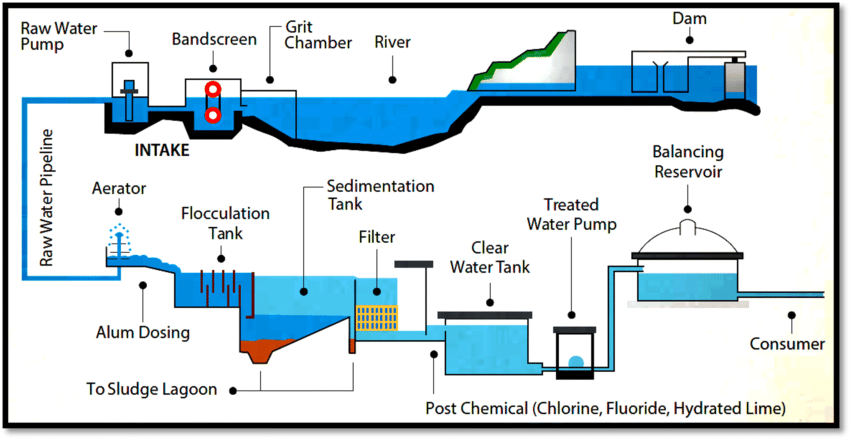
\includegraphics[scale=0.5]{WaterTreatment_9-01}
\caption{Conventional water treatment} \index{Conventional water treatment}
\end{center}
\end{figure}
\subsection{Source water treatment}\index{Source Water Treatment}
\begin{itemize}
\item Source water treatment in reservoirs or lakes includes treatment to contain algae growth.
\item Algal bloom is a sudden large increase in algae caused by weather or by nutrients. 
\item Reasons for controlling algae:
\begin{itemize}
\item Taste and odor problems
\item Shortened filter runs
\item Changes in pH - increases during the day, decreases at night
\item When algae dies, causes depletion of dissolved oxygen (DO)
\item Organic loading which is DBP pre-cursor resulting in TTHMs.
\end{itemize}
\item Algaecide such as blue stone, copper sulfate (CuSO$_4$) is used to control algae. 
\item Action level for copper is 1.3 mg/L·	·

\item Copper sulfate dose is usually specified in terms of pounds/acre. 
\item 5.4 lbs/acre is common dosage - the rate of application is based on the surface area of the reservoir not the volume
\item For water with alkalinify of higher than 150 mg/L, citric acid has to be mixed with CuSO$_4$ for it to be effective
\item Applying far more copper sulfate than necessary is uneconomical and ecologically undesirable. Excessive amounts of copper can kill fish and other bottom organisms, and copper tends to accumulate in bottom sediments. 
\end{itemize}
\subsection{Screening}\index{Screening}
\begin{itemize}
\item River water (the source of water used in our discussion) frequently contains suspended and floating debris varying in size from small rags to logs. Screening is usually the first major step where by large and suspended debris in the source water including sticks, leaves etc. is removed from the water before it enters the plant. 
\item Removing these solids is primarily to prevent damage to downstream equipment including pumps, prevent deposition of this debris in open channels or pipes, or in treatment processes.
\item The most important criteria used in the selection of a particular screening system for are the screen opening size and flow rate. Other important criteria include costs related to operation and equipment, plant hydraulics, debris handling requirements, and operator qualifications and availability. 
\item Depending on the characteristics of the source water, variety of screening devices including trash rakes, bar screens and wire mesh screens may be used. Very small screens can be used to screen out elements including algae in the water.
\item Typical screening devices used include:
\begin{itemize}
\item Trash Screens (Rakes) - used to remove rough or large debris.  The bar spacing in Rakes range from 1.5 to 4 inches.
\item Traveling Water Screens (Bandscreens) - these are placed in a channel of flowing water to remove floating or suspended debris.
\begin{figure}[h]
\begin{center}
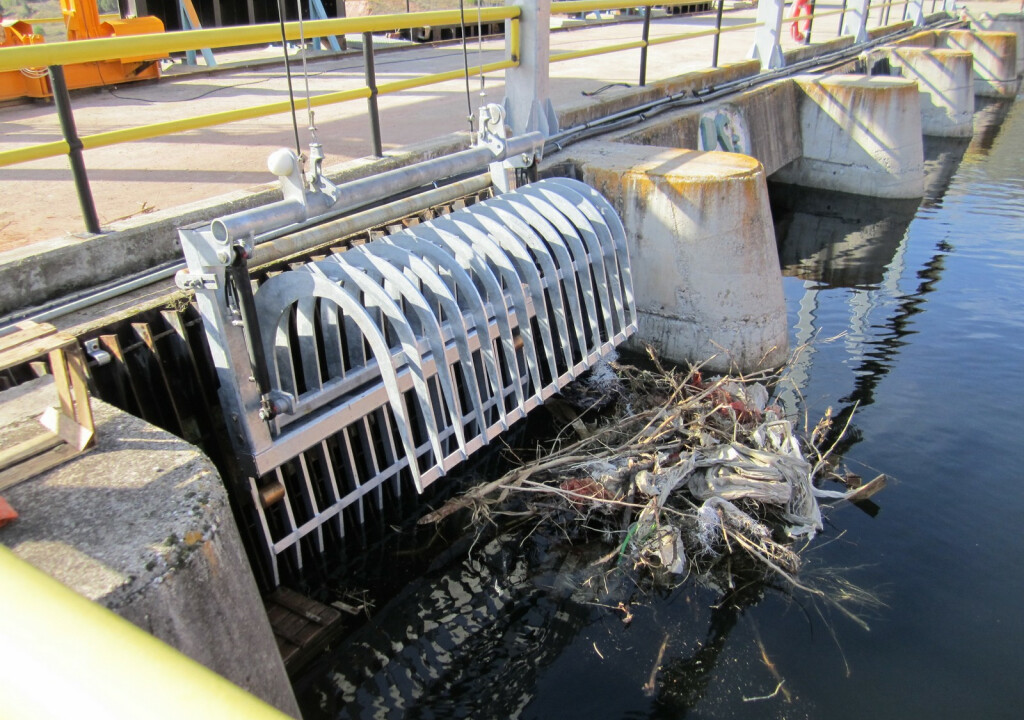
\includegraphics[scale=0.25]{TrashRakes}
\captionof{figure}{Trash rake}
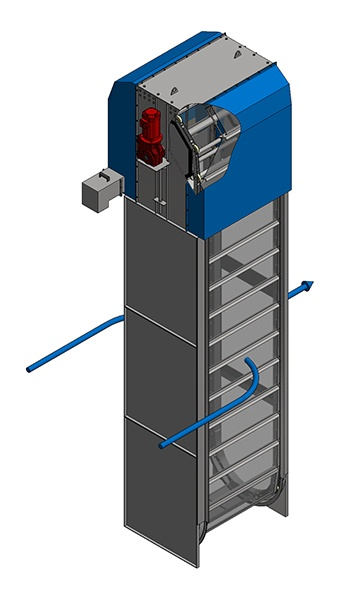
\includegraphics[scale=0.4]{TravellingScreen}
\captionof{figure}{Band screen}
\end{center}
\end{figure}
\end{itemize}

%\begin{center}
%\tcbox{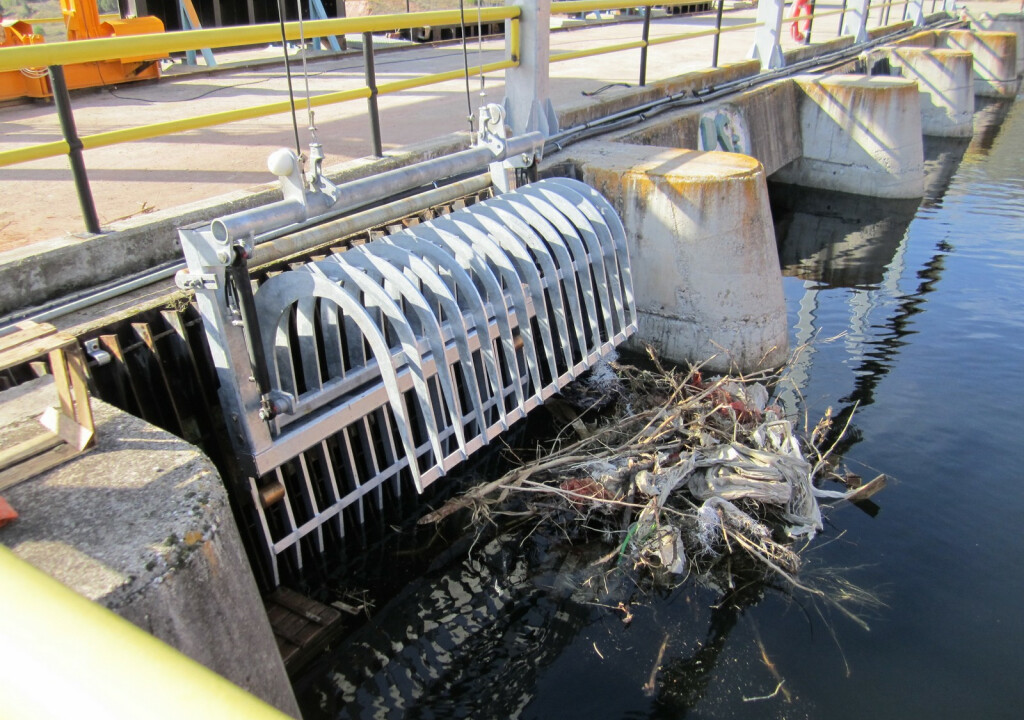
\includegraphics[width=6cm]{TrashRakes}}
%Trash Rakes
%\tcbox{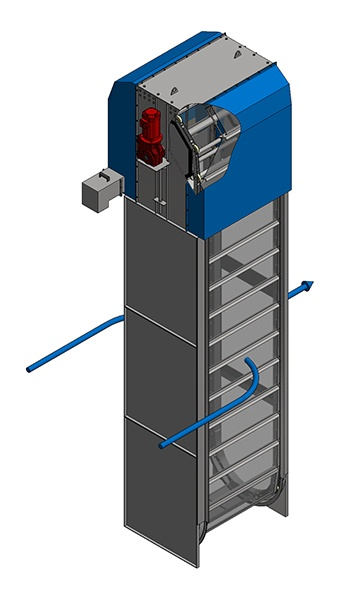
\includegraphics[width=6cm]{TravellingScreen}}
%\end{center}


\end{itemize}

\subsection{Coagulation and flocculation}\index{Coagulation and flocculation}
\begin{itemize}
\item A significant amount of suspended particles in the raw water are too small to be filtered or settled out in the sedimentation basin.  These particles, termed as colloids are non-settleable solids and include organic matter, silt, clay.
\item These particles impart turbidity and color to the water and may harbor pathogens and typically carry a negative electrostatic charge on its surface - negative \textbf{zeta potential}.  The like surface charge on these particles cause electrostatic repulsion (particles keep bouncing off one another) which makes these particles difficult to settle. 
\item Coagulation and flocculation are sequential processes both of which involve chemical addition.
\item For coagulation, either metal salt type coagulant - typically an aluminum salt such as alum or aluminum sulfate or an iron salt such as ferric or ferrous chloride or sulfate, polyaluminum chloride or a organic coagulant such as polyDADMAC or polyamine is used. The coagulant helps coalesce the non-settleable solids into larger particles.
\item Sodium aluminate is often used as an aide to alum coagulation particularly for cold water and during lime softening.
\item Coagulation is affected by changes in the water's pH, alkalinity, temperature, time, velocity and zeta potential.

\item The effectiveness of a coagulant is generally pH dependent. Water with a color will coagulate better at low pH (4.4-6) with alum.

\item Alkalinity is needed to provide anions, such as (OH$^-$) for forming insoluble compounds to precipitate them out. It could be naturally present in the water or needed to be added as hydroxides, carbonates, or bicarbonates.  Generally 1 part alum uses 0.5 parts alkalinity for proper coagulation.

\item The higher the temperature, the faster the reaction, and the more effective is the coagulation. Winter temperature will slow down the reaction rate

\item The coagulation process requires rapid mixing of the water upon the addition of the coagulant followed by a sufficient contact time prior to the flocculation step.
\item The flocculant which is added after the coagulation step is to make even larger, more compact and settleable - \textbf{floc}, from the coagulated solids.
\item Flocculants are typically long chain organic compounds - polymers with charged end groups.  \textbf{anionic polymers} have a negative end group whereas \textbf{nonionic polymers} have balanced - positive and negative end groups.
\item For the floc formed to remain intact, the polymer is gently "folded in" with the coagulated solids.  The flocculation is done in a flocculator which have a detention time of 5 -30 minutes and the water is mixed with the polymer using slow moving paddles.
\item Coagulant aids - chemicals which aid in the coagulation process and strengthening the flow include:
\begin{itemize}
\item Alakalinity enahncers - lime, Soda ash, caustic soda and sodium bicarbonate.
\item Weighting agents - calcimu carbonate and bentonite clay.  These are used in waters which are low in tubidity and high in color which under normal condition would have formed weak, slow settlling floc.
\item Activated sililca - sodium silicate activated by hypochlorous acid is often used as a coagulant aid with alum.
\end{itemize}


\end{itemize}

\item These will usually be used in conjunction with a primary coagulant such as ferric chloride, ferric sulfate, or alum.

\vspace{0.6cm}

\vspace{0.6cm}
\begin{figure}[H]
\includegraphics[scale=.13]{CEPTInitial} \hspace{0.7 cm}\includegraphics[scale=.13]{CEPTCoagulation}\hspace{0.7 cm}
\includegraphics[scale=.13]{CEPTFlocculation}\\
\hspace{0.8cm} \textbf{Untreated Water}\hspace{2.4 cm}\textbf{Coagulation}\hspace{3 cm}\textbf{Flocculation}\\	
\caption{Coagulation-flocculation graphic}
\label{Coagulation-flocculation graphic}
\end{figure}

\item Determining the amount and type of coagulant used changes based on a variety of process conditions and quality of water. For example, a heavy rain will greatly impact the influent, or raw, water in a municipal treatment plant.

\item The jar test is a standard method in which various amounts of coagulant and flocculation times are tested on a raw water sample. There are multiple samples to test before implementation into a larger volume of the water treatment process.

\begin{figure}[h]
\begin{center}
\includegraphics[scale=0.2]{JarTest}
\caption{Jar testing}
\label{table:Jartesting}
\end{center}
\end{figure}	

\end{itemize}
\subsection{Clarification/sedimentation}\index{Clarification/sedimentation}
\begin{itemize}
\item Clarification, or sedimentation, is the third step in conventional water treatment, after coagulation and flocculation and before filtration.
\item In the sedimentation basin the flocculated particles settle out under the influence of gravity.
\item In conventional sedimentation basins the solids drop out (settle) as the water slowly flows across the basin from the influent to effluent end.
\item Sedimentation basins are designed to create conditions in which the water flows very slowly through the basin, with minimal turbulence.
\item Conventional sedimentation basins are typically rectangular or cylindrical concrete or steel vessels which incorporate a horizontal flow of water.
\end{itemize}

			\begin{center}
				\includegraphics[scale=0.9]{RectangularClarifier}\\
				Cross section of a Rectangular Clarifier\\

				\includegraphics[scale=0.1]{Blank}\\
				\includegraphics[scale=0.6]{CircularClarifierAI}\\
				Schematic cross section of a circular clarifier\\
				%\includegraphics[scale=0.1]{Blank}\\
				%\includegraphics[scale=0.65]{CircularClarifier3}\\
				%Cross section of a circular clarifier\\
			\end{center}
				%\includegraphics[scale=0.03]{Blank}\\


\subsubsection{Clarifier Zones}\index{Clarifier Zones}		
	\begin{itemize}
		\item Inlet Zone: is where the water enters the end of a rectangular tank, or the center of a circular or square tank. The Inlet Zone is designed to accomplish two objectives:
			\begin{enumerate}
				\item Reduce the velocity (dissipate 									energy in the incoming water).  This is accomplished by the inlet baffle.
				\item Distribute the flow evenly using baffles in front of the influent baffle.
			\end{enumerate}
				
		\item Settling Zone: This is the largest portion of the tank where the water is flowing very slowly allowing the solids to settle.  The clarifier is said to be short circuiting if 		the velocity of the water is greater in some sections than in others. The water passing through the higher velocity region will have a reduced detention time and settleable solids will carry through with this water as it exits the clarifier.
		\item Sludge Zone: Sludge zone is the bottom of the tank where the 	settled solids collect and compact. Sludge rakes push the sludge to one end or the center of the tank so that it can be pumped out. 
		\item Skimming Zone: The skimming zone is at the surface of the tank for removing scum removing
		lighter solids which float to the surface.  
		\item Outlet Zone: This is the part of the clarifier where the settled water leaves the clarifier.  A channel called the effluent launder collects the effluent flow and directs it to the clarifier effluent piping. Weirs are installed along the edge of the effluent launder channel to skim the water evenly off the surface of the tank. 
		\end{itemize}


\subsection{Filtration}\index{Filtration}
\subsubsection{Process Basics}\index{Process Basics}
\begin{itemize}
\item The SWTR requires the filtration of surface water and groundwater under the direct influence of surface water.
\item Filtration is the mechanical removal of turbidity particles by passing the water through a porous medium, which is either a granular bed or a membrane.
\item The process of filtration involves straining, settling, and adsorption.
\item Filtration does not remove dissolved solids and by itelf is not effective for the removal of bacteria.
\item In filtration, solids are removed physically by:
\begin{itemize}
\item Straining – trapping particles, and 
\item Adsorption.
\end{itemize}
\item The filtration based treatment process can be either:
\begin{enumerate}
\item Conventional - which is a four step treatment process that consists of the treatment steps of coagualation, flocculation, sedimentation and rapid sand filtration.  
\item Direct - where the sedimentation step is omitted. It is for areas with high quality of water and allows for cost and space savings by eliminating the need for sedimentation basins.  
\end{enumerate}
\begin{figure}[H]
\begin{center}
\includegraphics[scale=0.75]{ConventionalFiltration}\\
\captionof{figure}{Conventional filtration}%\caption{}
\label{Conventional filtration}
\end{center}
\end{figure}

\begin{figure}[H]
\begin{center}
\includegraphics[scale=0.75]{DirectFiltration}\\
\captionof{figure}{Direct filtration}%\caption{}
\label{Direct filtration}
\end{center}
\end{figure}
\item Filters can also be classified as:
\begin{itemize}
\item Gravity – open to atmosphere and rely on the depth of water above the filter media to provide
the driving force to pass water through the media.
\item Pressure – utilize a pressure vessel to contain the media and can operate with a much higher driving force to pass water through the media.
\end{itemize}
\item Rapid gravity filters and slow sand filters are the two major types of filters used for water treatment.

\item Rapid filtration has following features that allow it to operate at higher water loading rates:
\begin{enumerate}
\item A filter bed of granular material that has been processed to a more uniform size than typically found in nature.
\item Use of a coagulant to precondition the water, and
\item Mechanical and hydraulic systems to efficiently remove collected solids from the bed.
\end{enumerate}
\item The rapid filtration
cycle consists of two stages: 
\begin{enumerate}
\item Filtration stage, when water flows downward through the filter bed and particles collect within the bed, and 
\item Backwash stage, water flows in the direction opposite to remove the particles that have collected in the filter bed. Efficient removal of collected solids is a key component of rapid filtration systems, so while the backwashing stage is very short compared to the filtration stage, it is a very important part of the filtration cycle.
\end{enumerate}

\item Rapid filtration is classified by the level of pretreatment, as presented in Figure ~\ref{figure:RapidFiltrationbyPretreatmentLevel}. The most important factors that determine the required level of pretreatment are the raw-water quality and the preference and resources of the operating utility.

\begin{figure}[H]
\begin{center}
\includegraphics[scale=0.8]{RapidFiltrationbyPretreatmentLevel1}\\
%\captionof{figure}{Rapid Filtration by Pretreatment Level 0.8}%\caption{}
\end{center}

\caption{Rapid filtration by pretreatment level}  
                \label{figure:RapidFiltrationbyPretreatmentLevel} 
\end{figure}

\item In a slow sand filter there is a  layer - \textbf{Schmutzdecke} that develops on the top and is made up of microrganisms that feed on and break down organic material that is trapped on the surface of the filter. If the source water naturally contain low levels of nutrients, initial nutrient addition may be needed to develop this layer.

\item The Schmutzdecke enhances the particulate removal.  As the Schmutzdecke develops, the filter performance – as measured by the turbidity typically improves as the filter run progresses.

\item Filter media can consist of silica sand, greensand, anthracite coal, activated carbon,
and many other types of media. 
\item Filter media maybe a single media or mixed to provide improved filtration characteristics. 
\item Two most common types of granular media filters include dual-media filters such as anthracite coal and silica sand and tri-media which have anthracite coal, silica sand and fine garnet. 
\item Greensand media which incorporates potassium permanganate and manganese greensand which is the mineral called glauconite coated with manganese oxide.  Manganese greensand is a popular filtration media choice as it removes dissolved iron and manganese, hydrogen sulfide, radium and arsenic. Regeneration of traditional Greensand every six to twelve months with permanganate is recommended.
\item Activated carbon can be used as a topping for silica sand.  The activated carbon  does not only remove solids but also helps adsorb organic contaminants.
\item Pre-coat filters, utilize a slurry of raw water with diatomaceous earth (DE) as a pre-coat on a septum filter media which then captures the turbidity causing particles from raw water.  The filtration process is followed by a backwash cycle to remove the filtered cake buildup.  Precoat filtration is used to remove very small particulate matter, oil particles, and even bacteria from water. This method is practical only for relatively small quantities of water which contain low concentrations of contaminants.

\begin{figure}[H]
\begin{center}
\includegraphics[scale=.6]{RapidSandFilter} \hspace{0.7 cm}\includegraphics[scale=0.6]{SandFilter}\hspace{0.7 cm}\\
\textbf{Rapid Sand}\hspace{5 cm}\textbf{Slow Sand}\\
\vspace{0.8cm}
\includegraphics[scale=0.7]{DiatomaceousEarthFilter}\\
\textbf{Pre-coat - Diatomaceous Earth}\\
%\hspace{0.8cm} \textbf{Rapid Sand}\hspace{2.4 cm}\textbf{Slow Sand}\hspace{3 cm}\textbf{DE}\\	
\caption{Filter types}
\index{Filter types}
\end{center}
\end{figure}

\item Filters can also be classified as:
\begin{itemize}
\item Depth filtration – solids are removed within the granular material.  Example: Rapid granular bed filter
\item Cake filtration – solids are removed on the entering face of the granular material.  Example: Precoat
\end{itemize}
\item The Surface Water Treatment Rule describes five different types of filtration systems: 
\begin{itemize}
\item Conventional treatment
\item Direct filtration
\item Slow sand filtration
\item Diatomaceous earth filtration
\item Alternate filtration technologies such as bag filters and cartridge filters.
\end{itemize}
\item Besides using a filter media, process akin to filtration can also be accomplished using membranes. 
\item A membrane is a thin layer of material that will only allow certain compounds to pass through it. 
\item During operation, permeable components pass through the membrane and impermeable components are retained on the feed side. As a result, the product stream is relatively free of impermeable constituents and the waste stream is concentrated in impermeable constituents.
\item Which material will pass through the membrane is determined by the size and the chemical characteristics of the membrane and the material being filtered.
\item Membranes can be classified into two distinct physicochemical
processes: 
\begin{enumerate}
\item Membrane filtration which encompasses the use of:
\begin{enumerate}
\item Microfiltration (MF)membrane which function like a sieve. MF membrane pore size ranges from 0.1 to 1 micrometer ($\mu$m); therefore, they remove all particles bigger than 1 $\mu$m, including Cryptosporidium oocysts, Giardia cysts and all bacteria., and 
\item Ultrafiltration (UF) membranes which are similar to the microfiltration membranes except the pore size is smaller - 0.003 to 0.1 $\mu$m which removes very small particles including viruses and THM formation precursors.
\item Nanofiltration (NF) membranes which have nanometer (0.001 $\mu$m, or 1 nm) pore size and can remove all the particles above nanometer size - besides removing viruses, cysts, and bacteria they remove some dissolved substances including divalent ions such as Ca$^{+2}$ and Mg$^{+2}$,and are used for softening water and to reduce the concentration of organic matter to control disinfection by-product (DBP) formation.
\end{enumerate}
\item Reverse Osmosis (RO) where preferential diffusion of water through a semipermeable membrane in response to a concentration gradient.  
\begin{itemize}
\item In RO, the feed stream is a solution, or single-phase system, in which the constituents targeted for removal are truly dissolved solutes - ions such as sodium, chloride and dissolved NOM.
\item RO membranes are semipermeable - they function as sieves and selective diffusion membranes due to osmosis, allowing for specific dissolved substances to pass through. 
\item Osmosis is the passage of water through a semipermeable membrane from the lower concentration of the dissolved substances to the higher concentration to equalize the concentration on both sides of the membrane. The force with which water flows through the membrane is called osmotic pressure. The greater the difference in concentration on two sides of the membrane, the higher the osmotic pressure, and faster is the flow. In reverse osmosis, a pressure higher than the osmotic pressure is applied on the higher concentration side to force the water through the membrane in the reverse order. 
\item RO membranes  are used to treat seawater that has total dissolved solids (TDS) in the range of 3.5\% (35,000 mg/L) and other brackish water (TDS up to 3\%).  
\item RO is also capable of removing specific dissolved contaminants - pesticides, arsenic, nitrate, radionuclides.
\end{itemize}
\end{enumerate}

\begin{figure}[H]
\begin{center}
\includegraphics[scale=0.8]{MembraneProcesses}\\
\captionof{figure}{Membrane processes}%\caption{}
\label{Membrane processes}
\end{center}
\end{figure}
%\item Filter media in a rapid sand filter refers to the granular material used to remove particles from the filter influent. 
%\item Typical filter media in a rapid sand filter include sand (of course), and sometimes a “cap” of coal or granular activated carbon (GAC) placed on top of the sand media layer. 
%\item Filters with a sand and coal/carbon cap are referred to as dual media filters. Some rapid sand filters also contain a thin layer of garnet sand. This layer also tends to improve filter performance.  
%\item Filters with a layer of garnet sand are referred to as mixed media filters.
%\item Rapid sand filtration is the most common type of filtration used in water treatment. 
%\item Slow sand filtration is usually a feasible alternative for SWTR compliance only for small water systems with relatively high quality source water.
%\item Also, pre-treatment (example: coagulation/flocculation) and final disinfection are therefore needed. 
%
%
%
%\item Granular Bed and Pre-coat Filters are typically used for surface water treatment
%
%\item Media in Granular Bed filter is comprised of one or a combination of the following:
%\begin{itemize}
%\item Sand
%\item Anthracite
%\item Granular activated carbon
%\end{itemize}
%\item Pre-coat filters use a thin layer of very fine medium such as diatomaceous earth.  Precoat filtration is used to remove very small particulate matter, oil particles, and even bacteria from water. This method is practical only for relatively small quantities of water which contain low concentrations of contaminants.
%
%\item Gravity filters can be operated at different hydraulic rates
%\begin{itemize}
%\item Slow filters
%\item Rapid filters
%\end{itemize}
%


\end{itemize}
%\subsection{Conventional Treatment} \index{Conventional Treatment}
%
%\subsection{Direct Filtration} \index{Direct Filtration}
%
%\subsection{Slow Sand Filtration} \index{Slow Sand Filtration}
%
%Microfiltration membranes function like a sieve. There pore size ranges from 0.1 to 1 micrometer ($\mu$m); therefore, they remove all particles biggerthan 1 $\mu$m, including Cryptosporidium oocysts, Giardia cysts and all bacteria. They are successfully used for water treatment plants with less than12 million gallons per day capacity and low raw water turbidity.
%Ultrafiltration
%Ultrafiltration membranes are similar to the microfiltration membranes except the pore size is 0.003 to 0.1 $\mu$m to remove very small particles. Theyremove all particles bigger than this pore size, including viruses and THM formation precursors. They remove cysts and other pathogens by sixlogs, meaning 99.9999 percent removal. They are more expensive due to the smaller pore size. The finer the pore size, the more effective themembrane, and the more expensive it is.
%Nanofiltration
%Nanofiltration membranes have nanometer (0.001 $\mu$m, or 1 nm) pore size.  They remove all the particles above nanometer size. Besides removingviruses, cysts, and bacteria, they remove some dissolved substances.
%
%Reverse Osmosis
%Reverse osmosis membranes are semipermeable. They function as sieves and selective diffusion membranes due to osmosis, which allows some specific dissolved substances to pass through. Osmosis is the passage of water through a semipermeable membrane from the lower concentration of the dissolved substances to the higher concentration to equalize the concentration on both sides of the membrane. The force with which waterflows through the membrane is called osmotic pressure. The greater the difference in concentration on two sides of the membrane, the higher theosmotic pressure, and faster is the flow. In reverse osmosis, a pressure higher than the osmotic pressure is applied on the higher concentration sideto force the water through the membrane in the reverse order. These membranes will remove all the suspended particles larger than the pore sizeand only selective dissolved substances. These membranes remove substances like sodium, calcium, magnesium, and other metal compounds.They are used to treat seawater that has total dissolved solids (TDS) in the range of 3.5% (35,000 mg/L) and other brackish water (TDS up to 3%).
%
%
%
%
%
%There are common variations of the conventional treatment and direct filtration pro- cesses that can be used to meet regulatory water treatment goals, to improve process efficiency, and to reduce the operational complexity of surface water treatment pro- cesses. These include two-stage filtration and pressure filtration.
%
%
%
%\subsection{Rapid Sand Filters} \index{Rapid Sand Filters}
%
%
%\begin{figure}[H]
%\begin{center}
%\includegraphics[scale=0.8]{MembraneFiltration}\\
%\captionof{figure}{Membrane Filtration 0.8}%\caption{}
%\end{center}
%\end{figure}
%
%\begin{figure}[H]
%\begin{center}
%\includegraphics[scale=0.8]{NanoFilteringSoftening}\\
%\captionof{figure}{Nano Filtering Softening 0.8}%\caption{}
%\end{center}
%\end{figure}
%
%\begin{figure}[H]
%\begin{center}
%\includegraphics[scale=0.8]{SofteningLimeSoda}\\
%\captionof{figure}{Softening Lime-Soda 0.8}%\caption{}
%\end{center}
%\end{figure}
%
%\begin{figure}[H]
%\begin{center}
%\includegraphics[scale=0.8]{FeMnRemovalGroundwater}\\
%\captionof{figure}{FeMnRemovalGroundwater 0.8}%\caption{}
%\end{center}
%\end{figure}
%
%\begin{figure}[H]
%\begin{center}
%\includegraphics[scale=0.8]{GasVOCRemoval}\\
%\captionof{figure}{GasVOCRemoval 0.8}%\caption{}
%\end{center}
%\end{figure}
%
%\begin{figure}[H]
%\begin{center}
%\includegraphics[scale=0.8]{GasVOCRemoval}\\
%\captionof{figure}{GasVOCRemoval 0.8}%\caption{}
%\end{center}
%\end{figure}
%
%
%
%
%

\subsubsection{Operation}\index{Operation}
\begin{itemize}
\item The removal mechanism in filtration involves straining – trapping larger particles and through adsorbtion where particles attach themselves to the filter media
\item Typical Filtration Rates:
\begin{itemize}
\item Slow Sand: 0.05 gpm/ft$^2$ - 3 feet sand
\item Rapid Sand: 2 gpm/ft$^2$ – 3 feet sand
\item Pressure filters: 3 gpm/ft$^2$
\item High Rate: 2-6 gpm/ft$^2$ – various media configurations
\end{itemize}

\item After a period of operation – filter cycle, the filter headloss increases because of the accumulation of the trapped solids.
\item Rapid filters are cleaned by backwashing using an upward, high-rate flow of water

\item Coagulation-flocculation is not required for cake filtration whereas chemical treatment is required for depth filtration.
\item Backwashing involves reversing the flow of water through the filter causing water to travel from the bottom of the filter to the top. 
\item Backwash is done at specific rates in order to most effectively remove the particulate material.  Backwashing process can be augmented by introducing low pressure air into the backwash line.
\item Backwash rates of 12-15 gpm/ft$^2$ or higher are common for sand, and rates for anthracite may range from 8 to 12 gpm/ft$^2$.
\item Wastewater used for the backwash is collected and removed from the filter. 






\item \textbf{Operational Problems}

Two common issues include:

\begin{itemize}

 

%black, blue, brown, cyan, darkgray, gray, green, lightgray, lime, magenta, olive, orange, pink, purple, red, teal, violet, white, yellow.

%\colorbox{declared-color}{text}

%\begin{tcolorbox}[width=\textwidth,colback={red},title={With true corners},outer arc=0mm,colupper=white]   

%   Air binding – vacuum generated due to higher water outflow than inflow causes violent upheaval impacting the media bed, gravel and/or underdrain.

    %\includegraphics[scale=0.5]{frogimage.png}

%\end{tcolorbox}   

\item \textbf{Air Binding} – vacuum generated due to higher water outflow than inflow causes violent upheaval impacting the media bed, gravel and/or underdrain.

 

\item \textbf{Mud balls} – these are formed as a result of inadequate backwashing and can cause the the filter to completely clog-up.

\end{itemize}
\end{itemize}

%\subsubsection{Greensand Filtration}\index{Greensand Filtration}
%\begin{itemize}
%\item 
%\end{itemize}
%\end{itemize}
%\subsubsection{Granulated activated carbon filter}\index{Granulated activated carbon filter}
%\begin{itemize}
%\item Granulated activated carbon filter\\
%\vspace{0.3cm}
%\begin{minipage}{.6\textwidth}
%\begin{itemize}
%\item Granulated Activated Carbon (\textbf{GAC}) filters have a layer of activated carbon on top of anthracite or sand.
%\item Activated carbon adsorbs various contaminants, such as tastes and odor-causing organics, THMs, and synthetic organics. 
%\item GAC is lighter than sand or anthracite and has an effective size of 0.55 to 0.65 mm. \item These filters have the problem of losing some carbon during the backwashing; therefore backwashing is properly controlled to prevent the excessive loss of GAC. 
%\item Commonly, backwashing causes 1 to 6 percent GAC loss per year.
%\item Solids carbon blocks when used in lieu of granular carbon are effective in Cryptosporidium and Giardia removal.
%\end{itemize}
%\end{minipage}
% \begin{minipage}{0.5\textwidth}
%        \centering
%       \includegraphics[scale=0.7]{GAC}
%    \end{minipage}\\
%
%\end{itemize}.

\section{Other treatment processes}
\subsection{Pre-chlorination}\index{Pre-chlorination}
\begin{itemize}
\item Pre-chlorination - chlorine is added to the incoming flow or, instead, added right before filtration.  Benefits of prechlorination include:
\begin{itemize}
\item Elimination of algae and other forms of aquatic life from the water so they won’t cause problems in the later stages of water treatment. 
\item Removal of tastes and odors
\item Control of biological growth throughout the water treatment system, thus preventing growth in the sedimentation tanks (where solids are removed from the water by gravity settling) and the filtration media (the filters through which the water passes after sitting in the sedimentation tanks). 
\item Oxidation of iron, manganese and/or hydrogen sulfide present in the water into a precipitate which can be removed in the sedimentation and filtration steps.
\end{itemize}
\end{itemize}

\subsection{Packed tower air stripping}\index{Packed tower air stripping}
\begin{itemize}
\item Water is sprayed on the top of a packed bed while air is blown at the bottom.
\item The packing provide the interface for the transfer of the contaminants from water into the air phase.
\item Air stripping is for removing:
\begin{itemize}
\item Volatile solids compounds
\item Carbon dioxide
\item Hydrogen sulfide
\item Ammonia
\end{itemize}
\end{itemize}
\begin{figure}[H]
\begin{center}
\includegraphics[scale=0.65]{AirStripping}\\
\captionof{figure}{Air stripper}%\caption{}\\
\end{center}
\end{figure}

\subsection{Aeration}\index{Aeration}
\begin{itemize}
\item In the aeration process the water is either pumped up into the air or allowed to fall over an aeration device

\item Aeration as a water treatment practice is used for the following operations:
\begin{itemize}
\item carbon dioxide reduction (decarbonation)
\item oxidation of iron and manganese found in many well waters (oxidation tower).  During aeration, iron and manganese get oxidized into an insoluble precipitate which is removed during filtration.
\item ammonia and hydrogen sulfide reduction (stripping)
\item Aeration is also an effective method of bacteria control.
\end{itemize}
\item Two general methods may be used for the aeration of water:
\begin{itemize}
\item Water-fall aeration Many variations of the water-fall principle are used for this type of aeration. The simplest configuration employs a vertical riser that discharges water by free fall into a basin.
\item Air diffusion aeration where air is diffused into a receiving vessel containing counter-current flowing water, creating very small air bubbles. This ensures good air-water contact for "scrubbing" of undesirable gases from the water.
\end{itemize}
\end{itemize}


\subsection{Iron and manganese sequestration}\index{Iron and manganese sequestration}
\begin{itemize}
\item Polyphosphates are used for sequestering iron and magnesium. Sequestration is the addition of chemicals to groundwater aimed at controlling problems caused by iron and manganese without removing them.
\item These chemicals are added to groundwater at the well head or at the pump intake before the water has a chance to come in contact with air or chlorine. This ensures that the iron and manganese stays in a soluble form.
\item If the water contains less than 1.0 mg/L iron and less than 0.3 mg/L manganese, using polyphosphates followed by chlorination can be an effective and inexpensive method for mitigating iron and manganese problems. 
\item No sludge is generated in this method. Below these concentrations, the polyphosphates combine with the iron and manganese preventing them from being oxidized. 
\item Any of the three polyphosphates (pyrophosphate, tripolyphosphate, or metaphosphate) can be used.
\item Applying sodium silicate and chlorine simultaneously has also been used to sequester iron and manganese. However, while this technique is reliable in the case of iron treatment, it has not been found to be effective in manganese control.  
\end{itemize}

\subsection{Fluoridation and defluoridation}\index{Fluoridation and defluoridation}
Fluoridation is the use of fluoride in the drinking water. Fluoride is an important component of bones and teeth. Fluoride deficiency causes weaker bones and tooth decay. Too much fluoride causes skeletal and dental fluorosis, resulting in brittle bones and mottled teeth, respectively.  An effective daily dose of fluoride is 0.9 to 1.7 mg/L. A dose less than 0.7 mg/L does not do the job, and more than 4.0 mg/L can cause fluorosis leading to irreversible demineralization of bone and tooth tissues.\\

The U.S. Department of Health and Human Services Agency (HHS) is recommending that water systems practicing fluoridation adjust their fluoride content to 0.7 mg/L, as opposed to the previous temperature-dependent optimal levels ranging from 0.7 mg/L to 1.2 mg/L.\\

EPA has set the maximum contaminant level for fluoride in the drinking water at 4mg/L \index{Fluoride!MCL}. Additionally, a secondary standard of 2.0 mg/L \index{Fluoride!SMCL} is intended as a guideline for an upper boundary level in areas which have high levels of naturally occurring fluoride.\\

Theoretically, any compound that forms fluoride ions in water solution can be used for increasing the fluoride content of a water supply. Most commonly used chemicals for this purpose include:\\
\begin{itemize}
\item Fluorosilicic acid fluorosilicic acid, as hexafluorosilicic acid (H$_2$SiF$_6$) which is a water-based solution used by most water systems in the United States. Fluorosilicic acid is also referred to as hydrofluorosilicate, FSA, or HFS.
\item Sodium fluorosilicate as disodium hexafluorosilicate (Na$_2$SiF$_6$) which is a dry salt additive, dissolved into a solution before being added to water, and
\item Sodium fluoride, a dry salt additive, typically used in small water systems, dissolved into a solution before being added to water.
\end{itemize}



In certain areas that have a naturally high level of fluoride in the groundwater defluoridation may have to occur.  Defluoridation methods include:
\begin{itemize}
\item Precipitation method utilizes chemical such as aluminum salts (i.e. alum) and lime.
\item  Ion-Exchange Methods utilizes different ion-exchange materials studied include bone, bone char and anion and cation exchange resins.
\item  Adsorption method uses chemical and physical adosrbents including activated carbon and alumina (Al$_2$O$_3$).  Activated alumina is used to treat water with fluoride concentrations from 4-20 mg/L in an adsorption process.
\end{itemize}

\subsubsection{Fluoride Dosing Chemicals Safety}
\begin{itemize}
\item Rubber gloves, coveralls, and protective eyewear should be worn when handling fluoride. 
\item Solid forms of fluoride are the most problematic to operators, since inhaling fluoride dust is very dangerous.  A dust collector should be used and a respirator should be worn when handling fluoride powders. 
\item Liquid forms, such as hydrofluosilicic acid, can also be dangerous.  Hydrofluosilicic acid produces poisonous fumes which must be vented and which are irritating to the skin.  The liquid itself can cause burns when allowed to touch skin.
\item The most extreme safety problem when dealing with fluoride is fluoride poisoning, which can be fatal.  However, fluoride poisoning occurs only when a large amount of fluoride - approximately one tablespoon - is ingested.  This is an amount much larger than would normally be inhaled while handling dry fluorides.  \item Accidental ingestion of fluoride chemicals can occur through contaminated food and drink.  The operator should always wash his hands after handling fluoride chemicals and should not eat, drink, or smoke in areas where fluorides are used or stored.\\
\end{itemize}

\subsection{Hardness removal}\index{Hardness removal}
\begin{itemize}
\item In almost every raw water supply, hardness is present as calcium and magnesium bicarbonate - (Ca/Mg)HCO$_3$, often referred to as carbonate hardness or temporary hardness. These compounds result from the action of acidic, carbon dioxide laden rain water on naturally occurring minerals in the earth, such as limestone.

CO$_2$ + H$_2$O = H$_2$CO$_3$\\

H$_2$CO$_3$ + CaCO$_3^-$ = Ca(HCO$_3$)$_2$

\item Hardness may also be present as a sulfate or chloride salt, referred to as noncarbonate or permanent hardness. These salts are caused by mineral acids present in rain water or the solution of naturally occurring acidic minerals.

\item Softening removes hardness and alkalinity making the product water more corrosive.  
\item It may be necessary to add corrosion-inhibiting materials to the finished water to protect the distribution system and prevent possible simultaneous compliance issues with other regulations like the Lead and Copper Rule.
\item Another option is to bypass a portion of water around the softening process and blending the treated and untreated waters are blended to produce an effluent with a total hardness around 50 to 75 mg/L as CaCO$_3$. 

\item Two common methods used to reduce hardness:
\begin{enumerate}
\item Cation exchange:
\begin{itemize}
\item In this process the calcium (Ca$^{+2}$) and magnesium (Mg$^{+2}$) ions that cause water hardness are replaced or exchanged with with a non-hardness ion like sodium. 
\item The exchange medium can be natural “zeolites” or synthetic resin beads that resemble wet sand and hold loosley the sodium ions provided by dissolving sodium chloride salt.
\item As hard water passes through a softener, the calcium and magnesium trade places with sodium ions. 
\item Eventually when the exchange medium becomes coated with calcium and magnesium ions, it must be recharged or regenerated.
\end{itemize}
\item Precipitation Softening
\begin{itemize}
\item Here the water is treated with lime or a combination of lime and soda ash (sodium carbonate, Na$_2$CO$_3$). 
\item These chemicals react with the hardness and natural alkalinity in the water to form insoluble compounds (precipitate) which are removed from the water by sedimentation and, usually, filtration.
\item Waters with moderate to high hardness and alkalinity concentrations (150-500 ppm as CaCO$_3$) are often treated in this fashion.
\begin{itemize}
\item Lime removes bicarbonates - which cause carbonate hardness. 
\item Soda ash is used to remove chemicals that cause non-carbonate hardness.
\end{itemize}
\item The addition of lime as either hydrated lime (calcium hydroxide - Ca(OH)$_2$) or as quicklime (CaO) results in:
\begin{itemize}
\item Increases the pH of water
\item Reaction with calcium bicarbonate Ca(HCO$_3$)$^-$ typically the major source of hardness converting it to CaCO$_3$.  For each molecule of calcium bicarbonate hardness removed, one molecule of lime is used. 
\item As the pH increases further, additional Ca(OH)$_2$ will then react with magnesium bicarbonate Mg(HCO$_3$) ultimately converting it to magnesium hydroxide (Mg(OH)$_2$.  For each molecule of magnesium bicarbonate hardness removed, two molecules of lime are used.
\item Calcium is removed in the 9.0-9.5 pH range and the pH needs to be at least 10.6 to remove magnesium.
\item Both CaCO$_3$ and Mg(OH)$_2$ have limited solubility in water and precipitate out.
\item Because CaCO$_3$ and Mg(OH)$_2$ precipitates are very slightly soluble, some hardness remains in the water--usually about 50 to 85 mg/l (as CaCO$_3$). This hardness level is desirable to prevent corrosion problems associated with water being too soft and having little or no hardness.
\end{itemize}
\item Use of lime along with soda ash  with results in:
\begin{itemize}
\item The magnesium non-carbonate hardness such as Mg(SO$_4$) is converted by lime to Mg(OH)$_2$ and Ca(SO$_4$) - a form of calcium non-carbonate hardness 
\item The calcium non-carbonate hardness - CaSO$_4$ is converted by soda ash to CaCO$_3$.  
\item For each molecule of non-carbonate calcium hardness removed, one molecule of soda ash is used.
\item For each molecule of non-carbonate magnesium hardness removed one molecule of lime plus one molecule of soda ash is used.
\item When water has minimal magnesium hardness, only calcium needs to be removed. Only enough lime and soda ash are added to water to raise pH to between 10.3 and 10.6, and calcium hardness will be removed from the water (but minimal magnesium hardness will be removed).
\item Extra lime addition is required to raise the pH above 10.6 to precipitate Mg(OH)$_2$ out of the water.
\item To improve magnesium reduction, which also improves silica reduction, sodium aluminate is added.  The sodium aluminate provides hydroxyl ion (OH$^-$) needed for improved magnesium reduction, without increasing calcium hardness in the treated water.  Additonal benefits of adding sodium aluminate comes from its formation of aluminum hydroxide which aids floc formation, conditions sludge blanket and helps reduce silica.
\end{itemize}
\item The portion of raw water may be bypassed 
\item Precipitation softening is often done in conjunction with coagulation and flocculation.
\item The precipitate formed is separated in the sedimentation tank as sludge.
\item The high pH, softened water produced is corrosive and \textbf{Recarbonation} \index{Recarbonation} of the softened water using carbon dioxide (CO$_2$) is conducted to lower the pH and thus its corrosivity.  
\item Lime softening produces large quantity of sludge.
\item \textbf{The reaction of quicklime with water leading to the formation of Ca(OH)$_2$ releases large quantity of heat and is dangerous if left uncontrolled.  Also, quicklime should never be stored with alum as the water of hydration in alum will react with quicklime causing an explosion}
\end{itemize}
\end{enumerate}
\end{itemize}

\begin{figure}[]
\begin{center}
\includegraphics[scale=0.48]{PrecipitationSOftening}\\
\captionof{figure}{Precipitation Softening}%\caption{}\\
\label{Precipitation softening}
\end{center}
\end{figure}

\subsection{Corrosion control}\index{Corrosion control}
\begin{itemize}
\item Corrosion is the gradual deterioration or destruction of metal surfaces by chemical and electrochemical processes.
\item As corrosive water stands or seals in pipes or tanks, it leaches metals from the piping, tanks, well casing, or other metal surfaces that water is in contact.
\item Corrosion can happen both from the inside of pipes and fittings and from the outside - because of the action of the external environment - including soils.
\item Lead and copper in service lines and household plumbing leach into the drinking water because of the corrosivity of water. 
\item Lead is a toxic metal that can be harmful to human health even at low exposure levels. Lead is persistent and can bioaccumulate in the body over time. 
\item The corrosivity of water will depend on the material of construction of the distribution system components and characteristics of water - water is less corrosive at higher pH and alkalinity.
\item Corrosion potential of the water on the distribution system components can be mitigated by chemical treatment:
\begin{itemize}
\item Adding alkalinity in the form of lime, soda ash, or caustic soda to make the water stable or slightly scale-forming. 
\item Orthophosphates are added to chemically react with lead and copper atoms forming lead and copper phosphate. The lead and copper phosphate is then electrochemically drawn back down onto the piping surface, where it forms a tough, water-resistant coating on the piping. 
\item Silicate compounds added to water also inhibit corrosion by forming a thin protective films on pipe walls.
\end{itemize}
\end{itemize}
\begin{table}[htp]
\captionsetup{justification=centering}
\scriptsize
\begin{tabular}{|p {2cm}|p {5cm}|p {7cm}|}
\hline
Treatment Method                               & How It Works                                                                                                                                                                                                                                             & What It Removes                                                                                                                                                                                                                                                                                                                                                                                                                                                    \\ \hline
Activated carbon filtration & As water flows through the filter contaminants   adsorb, or stick to, the surface of activated carbon particles.                                                                                                                        & Pesticides; organic compounds such as benzene and   carbon tetrachlo- ride; many odors; bacterial or colloidal iron or tannins when combined with continuous chlorination; radon; lead or copper if equipped   with special media; some other heavy metals in certain cases; chlorine;   chloramines; trihalomethanes. Filters with molded activated carbon blocks will treat Cryptosporidium and Giardia.
 \\ \hline

Reverse osmosis (RO)          &Contaminants are removed by forcing water through a   membrane which has microscopic holes. Water molecules pass through the   membrane but larger particles cannot. The membrane is flushed to remove   trapped contaminants.        & Certain tastes; some pesticides; high chloride content;   fluoride; nitrate; lead, copper, and other heavy metals; arsenic; Cryp tosporidium; viruses.                                                                                                                                                                                                                                                       \\
                                               &                                                                                                                                                                                                                                                          &                                                                                                                                                                                                                                                                                                                                                                                                                                                                    \\ \hline
Ion exchange water softening                   & As water passes through a resin   bed in the softener, calcium and magnesium in the water are exchanged for   sodium or potassium which do not create the nuisance problems associated with   hard water.                                                & Hard water (calcium and   magnesium); dissolved iron; manganese; will treat cadmium, copper and zinc if   operated properly.                                                                                                                                                                                                                                                                                                                                       \\ \hline


Sediment filtration                            & As water passes through a filter   made of sand, filter paper, compressed glass wool or other straining material   suspended particles such as sand, soil or other particles are trapped on   the filter.                                              & Sediment; acidic water when   preceded by soda ash feed; dissolved iron or manganese when preceded by   continuous chlorination, ozonation or aeration; turbidity.                                                                                                                                                                                                                                                                                             \\ \hline


Distillation & Water is heated to create steam which is then condensed to be collected   as treated water. Contaminants removed remain in the heating chamber or boil   off into the atmosphere. & Sediment; high salt content; high total dissolved solids; pesticides if   properly equipped with gas vent; fluoride; nitrate; lead, copper and other   heavy metals; arsenic; bacteria. 
\\ \hline

Aeration                                       & Oxygen is introduced into the water by an aerator. This oxidizes contaminants such as iron and manganese,   causing them to form solids which can then be filtered out of the water.   & Dissolved iron or manganese when followed by sediment filtration; may help reduce rotten egg odor from   dissolved hydrogen sulfide gas; radon.                                                                                                                                                                                                                                                                                                                  \\ \hline

De-Aeration                & Mix air with water to remove dissolved gases from the water. Aeration and                                                                                                                                                                              &Dissolved   hydrogen sulfide gas; radon. De-aeration equipment sometimes are very similar, but are designed for different   treatment goals.                                                                                                                                                   
\\ \hline

Continuous Chlorination       & Chlorine is fed or injected into the water to   kill bacteria and other microbial contaminants, as well as to oxidize iron   and manganese causing them to form solids which can then be filtered out.                             & Dissolved iron or manganese when   followed by sediment filtration; rotten egg odor from dissolved hydrogen   sulfide gas or sulfate-reducing bacteria (followed by activated carbon                                                                                                                                                                                                                                                                              filtration);   bacterial or colloidal iron or tannins when combined with activated carbon   filtration; bacteria; Giardia; viruses.                                                                                                                                                                                                                                                                                                                                \\ \hline 

Ultraviolet (UV) radiation    &As water passes through the system, a special lamp produces ultraviolet   light that kills bacteria and other microbial contaminants.
                                               &                                                                                                                                                                                                                                                          \\ \hline

Ozonation                     & Water enters a system where ozone is produced and mixed with the water,   a chemical form of pure oxygen,                                                                                                                                                                                     & Bacteria; Giardia; Cryptosporidium; viruses;   Ozonation destroys bacteria and other   microbial pathogens and oxidizes compounds such as iron and manganese causing   them to form solids which can then be filtered out using sediment filtration.
\\ \hline

Ultra,   micro, and nano filtration            & As water passes through a   filter, suspended particles are trapped on the filter. Particles removed   depends upon the size of the pores in the filter. Pore sizes from smallest to   largest are nanofiltration, ultra filtration and microfiltration. & Cryptosporidium; Giardia; viruses.                                                                                                                                                                                                                                                                                                                                                                                                                                 \\ \hline
\end{tabular}
\caption{Summary of water treatment methods} \index{Treatment!Summary of water treatment methods}
\label{Summary of water treatment methods}
\end{table}

\section{Best Available Technology (BAT)} \index{Best Available Technology (BAT)}

Below is the summary of BATs - the very best (state-of-the-art) control and treatment measures that have been developed, or are capable of being developed, and that are economically achievable, identified in the California Code of Regulations. 

\subsection{BATs for inorganics} \index{Best Available Technology (BAT)!Inorganics} 

% Please add the following required packages to your document preamble:
% \usepackage[normalem]{ulem}
% \useunder{\uline}{\ul}{}
\begin{table}[H]
\begin{tabular}{|l|l|}
\hline
\multicolumn{1}{|c|}{\textbf{Chemical}} & \multicolumn{1}{c|}{\textbf{Best Available Technologies (BATs)}} \\ \hline
Aluminum                                & 10                                                               \\ \hline
Antimony                                & 2, 7                                                             \\ \hline
Arsenic                                 & 1, 2, 5, 6, 7, 9, 13                                             \\ \hline
Asbestos                                & 2, 3, 8                                                          \\ \hline
Barium                                  & 5, 6, 7, 9                                                       \\ \hline
Beryllium                               & 1, 2, 5, 6, 7                                                    \\ \hline
Cadmium                                 & 2, 5, 6, 7                                                       \\ \hline
Chromium                                & 2, 5, 6$^a$ , 7                                                    \\ \hline
Cyanide                                 & 5, 7, 11                                                         \\ \hline
Fluoride                                & 1                                                                \\ \hline
Mercury                                 & 2 b , 4, 6 $^b$ , 7 b                                               \\ \hline
Nickel                                  & 5, 6, 7                                                          \\ \hline
Nitrate                                 & 5, 7, 9                                                          \\ \hline
Nitrite                                 & 5, 7                                                             \\ \hline
Perchlorate                             & 5, 12                                                            \\ \hline
Selenium                                & 1, 2 $^c$ , 6, 7, 9                                                 \\ \hline
Thallium                                & 1, 5                                                             \\ \hline
\end{tabular}
\end{table}
$^a$ BAT for chromium III (trivalent chromium) only.\\
$^b$ BAT only if influent mercury concentrations <10 $\mu$g/L.\\
$^c$ BAT for selenium IV only.\\

where:\\
1 = Activated Alumina\\
2 = Coagulation/Filtration (not BAT for systems <500 service connections)\\
3 = Direct and Diatomite Filtration\\
4 = Granular Activated Carbon\\
5 = Ion Exchange\\
6 = Lime Softening (not BAT for systems <500 service connections)\\
7 = Reverse Osmosis\\
8 = Corrosion Control\\
9 = Electrodialysis\\
10 = Optimizing treatment and reducing aluminum added\\
11 = Chlorine oxidation\\
12 = Biological fluidized bed reactor\\
13 = Oxidation/Filtration\\

\subsection{BATs for microbiological contaminants} \index{Best Available Technology (BAT)!Microbiological contaminants} 
Best available technology (BAT) (for a public water system serving more than 10,000 persons), affordable technology (for a public water system serving 10,000 or fewer persons), treatment techniques, or other means available for achieving compliance with the E. coli MCL are as follows:\\
(a) Protection of wells from fecal coliform contamination by appropriate placement and construction;\\
(b) Maintenance of a disinfectant residual throughout the distribution system;\\
(c) Proper maintenance of the distribution system including appropriate pipe replacement and repair procedures, main flushing programs, proper operation and maintenance of storage tanks and reservoirs, cross connection control, and continual maintenance of positive water pressure in all parts of the distribution system;\\
(d) Filtration and/or disinfection of approved surface water, in compliance with Section 64650, or disinfection of groundwater, in compliance with Section 64430, using strong oxidants such as chlorine, chlorine dioxide, or ozone; and\\
(e) For a system using groundwater, compliance with the groundwater portion of a Drinking Water Source Assessment and Protection Program.


\subsection{BATs for radionuclides} \index{Best Available Technology (BAT)!Radionuclides} 
% Please add the following required packages to your document preamble:
% \usepackage[table,xcdraw]{xcolor}
% If you use beamer only pass "xcolor=table" option, i.e. \documentclass[xcolor=table]{beamer}
% \usepackage[normalem]{ulem}
% \useunder{\uline}{\ul}{}
\begin{table}[H]
\begin{tabular}{|l|p{8cm}|}
\hline
\textit{Radionuclide} & \textit{Best Available Technology} \\ \hline
Combined radium-226 and radium-228                                       & Ion exchange, reverse osmosis, lime softening                                        \\ \hline
Uranium                                                                   & Ion exchange, reverse osmosis, lime softening, coagulation/filtration                 \\ \hline
Gross alpha particle activity                                             & Reverse osmosis                                                                      \\ \hline
Beta particle and photon radioactivity                                    & Ion exchange, reverse osmosis                                                     \\ \hline
\end{tabular}
\end{table}

\section{Chemical feed systems} \index{Chemical feed systems}
\begin{itemize}
\item Chemical feed systems are designed for automated and precise injection (dosing) of chemicals into the water to be treated. 
\item Chemical feed systems are mainly employed for the following types of water treatment:
\begin{itemize}
\item Disinfection
\item Flocculation and Coagulation
\item Nutrient Removal
\item Sludge Conditioning
\item Alkalinity Supplementation
\item Corrosion Inhibition
\end{itemize}
\item The chemical feed systems is comprised of different components and is typically designed to ensure suitability with the chemical dispensed and the environment.
\item There are three types of chemicals used by chemical feed systems: 
\begin{enumerate}
\item Dry Chemicals: These chemicals are in dry, powdered form. Sodium bicarbonate, calcium hypochlorite, calcium chloride, algaecides, and soda ash are a few popular types of dry chemicals. Dry chemicals may or may not be mixed with liquids.
\item Liquid Chemicals: These are most common form of chemicals used due to the ease of use. Aluminum sulfate or liquid alum, 50\% sodium hydroxide, and caustic soda are a few liquid chemicals used regularly.
\item Gaseous Chemicals: Chlorine gas is widely used in water treatment for disinfection.
\end{enumerate}
\end{itemize}

%\subsection{Key Components of a Chemical Feed System} \index{Chemical feed systems!Components}
\subsection {Types of chemical feed systems}\index{Chemical feed systems!Types}

\begin{itemize}
\item Chemicals are fed into the water stream in different ways based on the required feed rate and feed pump output. 
\item Typically, solid and liquid chemicals can be fed in any of the following ways:
\begin{itemize}
\item Continuous Feed: This system is commonly used for liquid chemicals, which are continuously fed into the water tank. This feed system is commonly employed for deposit control in once-through systems, as well as domestic water chlorination. The continuous feed may be provided by a gravity drip feed, where the feed rate is regulated by a needle valve.
\item Shot/slug Feed: The chemical is shot/slug-fed by an on-off control on a feeder pump. It may also be discharged from a measuring chamber or a calibrated pump. This type of feeding is widely used in bio-oxidation basins or cooling systems with high system volume to blowdown ratio.
\end{itemize}
\item For gaseous chemicals dosing, the following two methods are utilized.
\begin{itemize}
\item Solution Feed: This type of feeding is seen in vacuum-type feeders, where gas is drawn to the piping system by vacuum. If there is any leak in piping then it leads to vacuum loss, and as a result, the system is shut down for supply. The vacuum feeders use ejectors to create a vacuum required for operation.
\item Direct Feed: In this feed, gas is fed into the flow stream to be treated. This involves the direct injection of gas under high pressure. This type of feeding is usually restricted to small applications, which have no regular water supply for solution feed.
\end{itemize}
\end{itemize}

\subsection{Delivery systems}\index{Chemical feed systems!Components!Delivery}
\begin{itemize}
\item Feed pumps carry chemicals for dosing.   
\item \textbf{Metering pumps} are the most common types of feed pumps used for \textbf{liquid} chemical feed systems. Types of chemical metering pumps used in the water industry include:
\begin{itemize}
\item Diaphragm Pumps: 
\begin{itemize}
\item A diaphragm pump consists of one or more pumping chambers alternately filled and discharged by the movement of flexible diaphragms and check valves on the inlet and outlet.
\item The diaphragm pump is composed of the following:
\begin{itemize}
\item A chamber used to pump the fluid
\item A diaphragm or diaphragms operated by either electric or mechanical means
\item Two valve assemblies: a suction valve assembly and a discharge valve assembly
\end{itemize}
\begin{figure}[H]
\begin{center}
\includegraphics[scale=1]{AODDPump}
\vspace{0.2cm}
\caption{Air operated double diaphragm pump} \index{Pump type!Diaphragm pump}
\end{center}
\end{figure}
\item These pumps are widely used to handle mostly all liquid chemicals, as well as sludges and slurries with ease.
\end{itemize}
\item Peristaltic Pumps:
\begin{itemize}
\item These pumps are also known as roller pumps because it uses a set of rollers to pump the fluid. 
\item The chemical fluid to be pumped is contained in a flexible tube, which is positioned inside a pump casing.
\item The rotors equipped with rollers compress the tube, thereby forcing the fluid to move towards the pipe. The pump comes to its original position after the fluid moves out. This whole process is known as peristalsis. 
\item Peristaltic pumps are suited for applications requiring small feed rates of < 0.1 gallons per hour.
\end{itemize}
\begin{figure}[H]
\begin{center}
\includegraphics[scale=0.4]{PeristalticPump}\\
\caption{Peristaltic pump} \index{Pump type!Peristaltic pump}
\end{center}
\end{figure}
\item Other Metering pumps include: Packed Plunger Pumps, Liquid Gravity Feeders and Jet Pumps (Eductors)
\end{itemize}




\item For dry chemicals the following types of feeder systems are used:
\begin{itemize}
\item Volumetric Feeders: These feeders dispense an accurate amount of powdered material. Volumetric feeders are generally used for feeding dry chemicals such as lime slaking, lime feed, clay feed, dry polymer, and so on.
\item Gravimetric Feeders: The feeders feed chemicals by weight. Gravimetric feeders assure accuracy within 1-2\%.
\end{itemize}

\begin{figure}[H]
\begin{center}
\includegraphics[scale=.6]{VolumetricChemicalFeeder} \hspace{0.7 cm}\includegraphics[scale=0.6]{GravimetricChemicalFeeder}\hspace{0.7 cm}\\
\vspace{0.2cm}
\hspace{1 cm}Volumetric Feeder\hspace{5 cm}Gravimetric Feeder\\
\caption{Dry chemical feeders}
\end{center}
\end{figure}


\item Gaseous chemicals are transferred using gas feeders. To ensure safety, particularly when used in an application involving chemical such as chlorine, these gas systems are used under vacuum. To use these systems, special equipment and arrangements need to be done. Self-contained breathing equipment, special containment chorine rooms, chlorine gas detectors, as well as chlorine air room scrubbers are some of the requirements.
\end{itemize}
\subsection {Chemical storage systems}\index{Chemical feed systems!Components!Storage}
Solution tanks are the chemical storage systems used for holding chemical solutions to be fed into the water. There are three types of chemical storage systems used:
\begin{itemize}
\item Bulk Storage: The storage tank of this type can hold liquid chemicals in bulk. The chemicals for treatment are delivered by a carrier or a vendor truck. The tank is usually positioned near the feed system.
\item Semi Bulk Storage: This type of storage is ideal for applications that do not use chemical feeds regularly. Semi bulk storage tanks are designed in such a way that the tanks can be stored easily by stacking above one another when not in use.
\item Drum Storage: This was one of the most popular methods of chemical storage until a few years back. Safe disposal of drums after the end of their lifespan was one of the key challenges faced by users. To avoid this, nowadays, reusable containers - totes are used.
\end{itemize}

\subsection{Accessories}\index{Chemical feed systems!Components!Accessories}

\begin{itemize}
\item Mixers: The job of the mixer is to rapidly disperse the chemical additives to ensure a uniform mixture.  A rapid (or flash) mixer utilizes specifically designed impeller to uniformly disperse and blend chemicals, such as coagulant aids, chlorine, and sulfur dioxide, into the process stream.  Flash mixer can be installed in a tank, process chamber or pipe.
\begin{figure}[H]
\begin{center}
\includegraphics[scale=.4]{FlashMixer1} \hspace{3 cm}\includegraphics[scale=0.27]{FlashMixer2}\\
\vspace{0.2cm}
\hspace{1 cm}In-line Flash Mixer\hspace{4.5 cm}Process Flash Mixer
\caption{Flash mixers}
\end{center}
\end{figure}
\item Timers: Timers used to control the function of mixers, as well as the feeding of chemicals.
\item Alarms: Alarms are typically used as monitoring systems for different components of the chemical dosing system. They can be set to monitor tank levels, chemical feed rates, pump status, and changed operating conditions. Alarms help to reduce damages caused due to dry running or change in operating variables, or some unspecified conditions.
\item Level Gauges: As the name indicates, these devices are used to monitor the level of chemicals in tanks.
\item Control Panels: The control panel may also contain lights that indicate the status of the pumps, various alarm conditions, and hour meters.
\end{itemize}

\subsection {Chemical control systems}\index{Chemical feed systems!Control systems}
Typical types of chemical control systems include:
\begin{itemize}
\item Manual Controls: This is one of the simplest, yet popular controls employed in the water industry. The output of the pump is set manually using dials or knobs, and the pump is put on or off using a manual switch. Sometimes, the power supply on the pump is put on or off for operating or closing the pump.
\item Automatic chemical dosing control instrumentation is usually set up as either a “feed forward” or a “feedback” loop. 
\begin{itemize}
\item An example of a feed forward loop would be a venturi flow meter which is located forward of the chlorine feed point sending a signal to change a chlorine dosage based on a change in flow. 
\item An example of a feedback loop would be a chlorine analyzer located downstream of the chlorine dosage point, changing the chlorine dosage based on a change in residual downstream of the chlorinator.
\end{itemize}
\item On-off Constant Rate Mode: In this type of pump control, the pump on and off is automated. This control is more apt for cooling towers or other similar applications that do not require a continuous or regular feed of chemicals. In short, it is most suitable for controlling acid feed rates at low or high pH setpoints.
\end{itemize}

% \begin{tcolorbox}[breakable, enhanced,
% colframe=blue!25,
% colback=blue!10,
% coltitle=blue!20!black,  
% title= Chapter Assessment]
% \begin{enumerate}
% \item What is the recommended loading rate for copper sulfate for algae control at an alkalinity greater than 50 mg/L?
% \begin{enumerate}
% \item 0.9 lb of copper sulfate per acre of surface area
% \item 1.9 lb of copper sulfate per acre of surface area
% \item 2-4 lb of copper sulfate per acre of surface area
% \item.4 lb of copper sulfate per acre of surface area
% \end{enumerate}

% \item The basic goal for water treatment is to \rule{2cm}{0.3pt}.
% \begin{enumerate}
% \item Protect public health
% \item Make it clear
% \item Make it taste good
% \item Get stuff out
% \end{enumerate}

% \item Greensand can be operated in either \rule{2cm}{0.5pt} regeneration or \rule{2cm}{0.5pt} regeneration modes.
% \begin{enumerate}
% \item Continuous or intermittent
% \item Fast or slow
% \item Hot or cold
% \item Constant or unusual
% \end{enumerate}

% \item The two most common types of chlorine disinfection by-products include:
% \begin{enumerate}
% \item TTHM and HAA5
% \item TTHA of HMM5
% \item Turbidity and color
% \item Chloride and fluoride
% \end{enumerate}

% \item GAC contactors are used to reduce the amount of \rule{2cm}{0.5pt} contaminants in water.
% \begin{enumerate}
% \item Inorganic
% \item Turbidity
% \item Particle
% \item Organic
% \end{enumerate}

% \item List the five types of surface water filtration systems.
% \begin{enumerate}
% \item Bag filtration, cartridge filtration, fine filtration, coarse filtration, media filtration
% \item Conventional treatment, direct filtration, slow sand filtration, diatomaceous earth filtration, membrane filtration
% \item Turbidity filtration, color filtration, bag filtration, fine filtration, media filtration
% \item None of the above
% \end{enumerate}

% \item Describe two primary methods used to control taste and odor?
% \begin{enumerate}
% \item Oxidation and adsorption
% \item Filtration and sedimentation
% \item Mixing and coagulation
% \item Sedimentation and clarification
% \end{enumerate}

% \item The adsorption process is used to remove:
% \begin{enumerate}
% \item Organics or inorganics
% \item Bugs or salts
% \item Organisms or dirt
% \item Color or particles
% \end{enumerate}

% \item The solid that adsorbs a contaminant is called the:
% \begin{enumerate}
% \item Adsorbent
% \item Adsorbate
% \item Sorbet
% \item Rock
% \end{enumerate}

% \item What is a method of reducing hardness?
% \begin{enumerate}
% \item Softening
% \item Hardening
% \item Lightning
% \item Flashing
% \end{enumerate}


% \item Bag and cartridge filters are used to remove which two pathogenic microorganisms?
% \begin{enumerate}
% \item Viruses and giardia
% \item Giardia and cryptosporidium
% \item Viruses and bacteria
% \item None of the above
% \end{enumerate}

% \item The process of cleaning a filter by pumping water up through the filter media is called \rule{2cm}{0.3pt} the filter.
% \begin{enumerate}
% \item Backwashing
% \item Rewashing
% \item Purging
% \item Lifting
% \end{enumerate}

% \item In a typical water treatment plant, alum would be added into the \rule{2cm}{0.3pt} mixer.
% \begin{enumerate}
% \item Speed
% \item Large
% \item Slow
% \item Flash
% \end{enumerate}

% \item When comparing conventional treatment with direct filtration, what process unit is in the conventional treatment plant that is not in the direct filtration plant?
% \begin{enumerate}
% \item Filter
% \item Clarifier
% \item Mixer
% \item Detention
% \end{enumerate}

% \item List the basic processes, in the proper order, for a conventional treatment plant.
% \begin{enumerate}
% \item Coagulation, flocculation, sedimentation, filtration
% \item Flocculation, coagulation, sedimentation, filtration
% \item Filtration, coagulation, flocculation, sedimentation
% \item Coagulation, sedimentation, flocculation, filtration
% \end{enumerate}

% \item The four most common oxidants include:
% \begin{enumerate}
% \item Chlorine, potassium permanganate, ozone, chlorine dioxide
% \item Chlorides, soap, air, coagulants
% \item Air, chemicals, sodium, chloride
% \item Flocculants, coagulants, sediments, granules
% \end{enumerate}

% \item  When operating a filter, one of the operational concerns is the difference between the pressure or head on top of the filter and the pressure or head at the bottom of the filter. This difference is called \rule{2cm}{0.3pt} pressure.
% \begin{enumerate}
% \item Different
% \item Differential
% \item High
% \item Low
% \end{enumerate}

% \item  What type of polymer is used to improve the efficiency of the sedimentation
% process?
% \begin{enumerate}
% \item Cationic
% \item Nonionic
% \item Anionic
% \item All of the above
% \end{enumerate}

% \item A(n) \rule{2cm}{0.3pt} polymer is commonly used as a coagulant.
% \begin{enumerate}
% \item Anionic
% \item Cationic
% \item Nonionic
% \item Ionic
% \end{enumerate}


% \item A(n) \rule{2cm}{0.3pt} polymer is used to enhance flocculation.
% \begin{enumerate}
% \item Anionic
% \item Cationic
% \item Nonionic
% \item Ionic
% \end{enumerate}

% \item Al$_2$(SO$_4$)$_3$ • 18H$_2$O is the chemical formula for:
% \begin{enumerate}
% \item Alum
% \item Iron
% \item Manganese
% \item Lead
% \end{enumerate}

% \item Particles that are less than 1 $\mu$m in size and will not settle easily and are called:
% \begin{enumerate}
% \item Light particles
% \item Colloidal particles
% \item Colored particles
% \item Flat particles
% \end{enumerate}

% \item The sedimentation portion of water treatment is also called a(n):
% \begin{enumerate}
% \item Clarifier
% \item Filter
% \item Adsorber
% \item Water treater
% \end{enumerate}

% \item Slowly agitating coagulated materials is the process of:
% \begin{enumerate}
% \item Flocculation
% \item Coagulation
% \item Sedimentation
% \item Filtration
% \end{enumerate}

% \item The process of decreasing the stability of colloids in water is called:
% \begin{enumerate}
% \item Flocculation
% \item Coagulation
% \item Sedimentation
% \item Clarification
% \end{enumerate}

% \item The chemical oxidation process in water treatment is typically used to aid in the
% removal of :
% \begin{enumerate}
% \item Organic contaminants
% \item Inorganic contaminants
% \item Large contaminants
% \item None of the above
% \end{enumerate}

% \item Flocculation, sedimentation, filtration, and adsorption are \rule{2cm}{0.3pt}
% processes.
% \begin{enumerate}
% \item Physical
% \item Chemical
% \item Biological
% \item Mechanical
% \end{enumerate}

% \item Oxidation, coagulation, and disinfection are \rule{2cm}{0.3pt} processes.
% \begin{enumerate}
% \item Physical
% \item Chemical
% \item Biological
% \item Mechanical
% \end{enumerate}

% \item A precipitate can be formed after which one of the following processes:
% \begin{enumerate}
% \item Oxidation
% \item Flocculation
% \item Filtration
% \item Adsorption
% \end{enumerate}

% \item Water that is safe to drink is called \rule{1cm}{0.5pt}  water.
% \begin{enumerate}
% \item Potable
% \item Palatable
% \item Good
% \item Clear
% \end{enumerate}
% \end{enumerate}
% \end{tcolorbox}
\chapterimage{QuizCover} % Chapter heading image

\chapter*{Chapter 5 Assessment}
% \textbf{Multiple Choice}
\section*{Chapter 5 Assessment}
\begin{enumerate}[1.]
\item What is the purpose of coagulation and flocculation?\\
a. control corrosion\\
b. to kill disease causing organisms\\
c. to remove leaves, sticks, and fish debris\\
d. to remove particulate impurities and suspended matter\\
\item How are filter production (capacity) rates measured?\\
a. Mgd/sq.ft.\\
b. Gpm/sq.ft.\\
c. Gpm\\
d. Mgd\\
\item Why should a filter be drained if it is going to be out-of-service for a prolonged period?\\
a. to allow the media to dry out\\
b. to save water\\
c. to prevent the filter from floating on groundwater levels\\
d. to avoid algal growth\\
\item Which of the following are commonly used coagulation chemicals?\\
a. hypochlorites and free chlorine\\
b. sodium and potassium chlorides\\
c. alum and polymers\\
d. bleach and HTH\\
\item How can an operator tell if a filter is NOT completely cleaned after backwashing?\\
a. the initial headloss is on the high side\\
b. the backwash rate was too slow\\
c. mudballs are NOT present\\
d. backwashing pumping rate is too low\\
\item Flocculation is defined as\\
a. the gathering of fine particles after coagulation by gentle mixing\\
b. clumps of bacteria\\
c. the capacity of water to neutralize acids\\
d. a high molecular weight of compounds that have negative charges\\
\item A multi-barrier water filtration plant that contains a flash mix, a coagulation/flocculation zone, sedimentation, filtration and a clear well is considered to be a\\
a. community special treatment plant\\
b. direct filtration plant\\
c. reverse osmosis plant\\
d. conventional filtration plant\\
e. traditional plant\\
\item The filtration unit process usually\\
a. is located at the beginning of a filtration plant\\
b. follows the coagulation/flocculation/sedimentation processes\\
c. is located after the clear well area\\
d. is located on the plant effluent line after the clearwell\\
\item Filters are generally backwashed when the loss-of-head indicator registers a certain set value, such as 6-ft, or upon a certain time, say 48-hours, or upon a rise in\\
a. alkalinity\\
b. a jar-test result\\
c. turbidity\\
d. temperature\\
\item What is a method of reducing hardness?\\
a. Softening\\
b. Hardening\\
c. Lightning\\
d. Flashing\\
\item The solid that adsorbs a contaminant is called the:\\
a. Adsorbent\\
b. Adsorbate\\
c. Sorbet\\
d. Rock\\
\item The adsorption process is used to remove:\\
a. Organics or inorganics\\
b. Bugs or salts\\
c. Organisms or dirt\\
d. Color or particles\\
\item Describe two primary methods used to control taste and odor?\\
a. Oxidation and adsorption\\
b. Filtration and sedimentation\\
c. Mixing and coagulation\\
d. Sedimentation and clarification\\
\item What is the recommended loading rate for copper sulfate for algae control at an alkalinity greater than $50 \mathrm{mg} / \mathrm{L}$ ?\\
a. 0.9 of copper sulfate per acre of surface area\\
b. 1.9 of copper sulfate per acre of surface area\\
c. 2-4 lb of copper sulfate per acre of surface area\\
d. 5.4 of copper sulfate per acre of surface area\\
\item The basic goal for water treatment is to\\
a. Protect public health\\
b. Make it clear\\
c. Make it taste good\\
d. Get stuff out\\
\item Greensand can be operated in either \rule{1.5cm}{0.5pt} regeneration or \rule{1.5cm}{0.5pt} regeneration modes.\\
a. Continuous or intermittent\\
b. Fast or slow\\
c. Hot or cold\\
d. Constant or unusual\\

\end{enumerate}




\part{Chapter 6}
\chapterimage{uvdisinfectionhero.jpg} % Chapter heading image

\chapter{Disinfection}
\nopagebreak
\begin{table}[H]
\begin{tabular}{| m{1cm} | m{15cm} |}
\hline
\multicolumn{2}{|l|}{\textbf{Expected   Range of Knowledge for Water Properties and Sources}}                                                                          \\ \hline
\multicolumn{2}{|l|}{\textit{Water   Distribution System Operator License Exams}}                                                                                      \\ \hline
D1 & Ability to   measure total chlorine                                                  \\ \hline
D1 & Ability to monitor   and interpret chlorine residual                                 \\ \hline
D1 & Knowledge of causes   of chlorine demand                                             \\ \hline
D1 & Knowledge of contact   time                                                          \\ \hline
D1 & Knowledge of   dechlorination techniques                                             \\ \hline
D1 & Knowledge of the   purpose of disinfection                                           \\ \hline
D1 & Ability to apply   disinfectant                                                      \\ \hline
D1 & Knowledge of water   main disinfectant techniques                                    \\ \hline
D1 & Knowledge of well   disinfection techniques                                          \\ \hline
D2 & Ability to choose the   proper disinfectant technique                                \\ \hline
D2 & Ability to recognize   when breakpoint has been met                                  \\ \hline
D2 & Knowledge of   advantages/disadvantages of chloramination                            \\ \hline
D2 & Knowledge of   chloramine compounds                                                  \\ \hline
D2 & Knowledge of chlorine   analysis techniques                                          \\ \hline
D2 & Knowledge of   disinfectant types and characteristics                                \\ \hline
D2 & Knowledge of factors   affecting chlorine disinfection                               \\ \hline
D2 & Knowledge of the   causes of DBPs                                                    \\ \hline
D2 & Knowledge of the   chlorine curve                                                    \\ \hline
D2 & Knowledge of the   definition of breakpoint chlorination                             \\ \hline
D3 & Ability to calculate   CT                                                            \\ \hline
D3 & Ability to recognize   abnormal levels of DBPs in the water distribution system      \\ \hline
D3 & Knowledge of chlorine   chemistry                                                    \\ \hline
D3 & Knowledge of DBP   compounds                                                         \\ \hline
D3 & Knowledge of DBP   formation                                                         \\ \hline
D3 & Knowledge of DBP   reduction methods                                                 \\ \hline

\end{tabular}
\end{table}

\newpage



\begin{table}[H]
\begin{tabular}{| m{1cm} |m{15cm} |}
\hline
\multicolumn{2}{|l|}{\textbf{Expected   Range of Knowledge for Water Properties and Sources}}                                                                      \\ \hline
\multicolumn{2}{|l|}{\textit{Water   Treatment Operator License Exams}}                                                                  \\ \hline
T1 & Knowledge of   acceptable chlorine residual levels                                   \\ \hline
T1 & Knowledge of   breakpoint chlorination chemistry                                     \\ \hline
T1 & Knowledge of chlorine   chemistry                                                    \\ \hline
T1 & Knowledge of common   chlorine compounds used for disinfection                       \\ \hline
T1 & Knowledge of   disinfectant byproduct formation                                      \\ \hline
T1 & Knowledge of   disinfectant properties and uses                                      \\ \hline
\end{tabular}
\end{table}
\newpage

\section{Background}\index{Disinfection!Background}
\begin{itemize}
\item The primary goal of water treatment is to ensure that the water is safe to drink and does not contain any disease-causing microorganisms. 
\item Disinfection refers to an operation to inactivate the microorganisms in water that can cause an infection or disease. These organisms are collectively referred to as pathogens and include many species of bacteria, fungus, protozoa, worms, viruses, etc.
\item The processes prior to disinfection - sedimentation and filtration, remove a large percentage of bacteria and other microorganisms from the water by physical means.
\item Disinfection \index{Disinfection}is different from sterilization, which is the complete destruction of all organisms which is expensive and unnecessary.
\item Water disinfection can be sub-divided as:
\begin{enumerate}
\item Primary disinfection \index{Disinfection!Primary disinfection}:
\begin{itemize}
\item Kills or inactivates bacteria, viruses, and other potentially harmful organisms in drinking water.
\item Disinfection prevents infectious diseases such as typhoid fever, hepatitis, and
cholera
\item Some disinfectants are more effective than others at inactivating certain
potentially harmful organisms.
\item Disinfection processes vary from water utility to water utility based on their
needs and to meet EPA treatment requirements.
\end{itemize}
\item Secondary disinfection \index{Disinfection!Secondary disinfection}:
\begin{itemize}
\item Maintenance of a disinfectant residual that prevents regrowth of microorganisms in the water distribution system between treatment and consumer.
\item Secondary disinfection maintains water quality by killing potentially harmful
organisms such as those that cause Legionnaire’s disease that may get in water as it moves through pipes.
\item Monochloramine is commonly used as a secondary disinfectant.
\end{itemize}
\end{enumerate}
\item Elements of an "ideal" disinfectant
\begin{itemize}
\item It must act in a reasonable time.
\item It must act as temperature or pH changes.
\item It must be nontoxic.
\item No harmful byproducts.
\item It must not add unpleasant taste or odor.
\item It must be readily available.
\item It must be safe and easy to handle and apply.
\item It must be easy to determine the concentration of.
\item It must be able to provide residual protection.
\item Pathogenic organisms must be more sensitive to the disinfectant than are non-pathogens.
\item It must be capable of being applied continually.
\item Versatile:  effective against all types of pathogens.
\item Fast-acting:  effective within short contact times
\item Robust: effective in the presence of interfering materials including particulates, suspended solids and other organic and inorganic constituents
\item Handy: easy to handle, generate, and apply (nontoxic, soluble, non-flammable, non-explosive)
\item Compatible with various materials/surfaces in WTPs (pipes, equipment)
\item Economical
\end{itemize}
\item In addition to the desirable characteristics of a disinfectant listed above, the disinfectant chosen must be able to kill off or deactivate pathogenic microorganisms by one of several possible methods, including:
\begin{enumerate}
\item Damaging the cell wall
\item Altering the ability to pass food and waste through the cell membrane
\item Altering the cell protoplasm
\item Inhibiting the cells’ conversion of food to energy
\item Inhibiting reproduction
\end{enumerate}
\item Most chemical disinfectants being strong oxidizers, aid the water treatment process by providing other benefits which include:  \begin{itemize}
\item Taste and odor control
\item Oxidize iron and manganese
\item Limit nuisance growths - algae 
\item Reduce mudball formation in filter media
\item Limit anaerobic sludge conditions
\item Improving coagulation
\end{itemize}

\end{itemize}

\section{Chlorination}\index{Chlorination}
\begin{itemize}
\item Despite potential drawbacks, chlorine is the disinfectant of choice.
\item In general, chlorination is effective, relatively inexpensive, and provides effective levels of disinfectant residual for safe distribution. 
\item Chlorine can be applied as:
\begin{itemize}
\item As a gas - elemental chlorine, $\mathrm{Cl}_{2}$:\\
\item Liquid (sodium hypochlorite) 
\item Solid (calcium hypochlorite)\\
each of these forms has advantages and disadvantages.
\end{itemize}
\end{itemize}
\subsection{Chlorine properties}\index{Chlorine properties}
\begin{itemize}
\item Chlorine is a yellowish-green gas at room temperature and atmospheric pressure
\item Chlorine gas can be pressurized and cooled to its liquid form for making it easy to ship and store. 
\item When liquid chlorine is released, it quickly turns into a gas that stays close to the ground (being heavier than air) and spreads rapidly.
\item While it is not explosive or flammable, as a liquid or gas it can react violently with many substances 
\item Chlorine is only slightly soluble in water (0.3 to 0.7\% by weight.) 
\item It has a characteristic disagreeable and pungent odor, similar to chlorine-based laundry bleaches, and is detectable by smell at concentrations as low as 0.2 to 0.4 ppm
\item It is about two and a half times as heavy as air
\item One volume of liquid chlorine yields about 460 volumes of chlorine gas. 
\item Liquid chlorine is amber in color and is about one and a half times as heavy as water 
\item Chlorine is an irritant to the eyes, skin, mucous membranes, and the respiratory system 
\end{itemize}

\subsection{Chlorine storage and safety}\index{Chlorine storage and safety}
\begin{itemize}
	\item Chlorine gas is lethal at concentrations as low as $0.1 \%$ air by volume. In nonlethal concentrations, it irritates the eyes, nasal membranes, and respiratory tract.
	\item Typically for smaller plants chlorine gas is shipped in  pressurized steel cylinders - 150 lb or 2000 lb (ton cylinder) size.  Larger plants may get their chlorine supply in rail tank cars.  \index{Chlorine cylinder}
	\item The daily chlorine usage is typically established based upon the weighing of the chlorine containers.
	\item The withdrawal rates from a chlorine cylinder is based on the temperature of the liquid in the cylinder, and thus the pressure of the gas. 
	\item As chlorine gas is withdrawn from the cylinder, it absorbs the heat from the surroundings.
	\item For low withdrawal rates, heat will be able to be transferred from the surrounding air to the container in time so that there is no drop in temperature or pressure, 
	\item If the chlorine withdrawal is larger, the air will not be able to transfer the heat quickly enough and the temperature (and pressure) of the chlorine will drop, thus resulting in a lower feed rate. 
	\item If high enough and prolonged enough, this can even result in ice formation around the outside of the container, further decreasing the withdrawal rate. 
	\item The most effective way to increase withdrawal rate from a single container is to circulate the surrounding air with a fan. Again, never apply heat to the containers.
	\item The maximum withdrawal rate for 100 or 150-pound cylinders should be limited to 40 pounds per day per cylinder. The maximum withdrawal rate for one-ton containers should be limited to 400 pounds per day per cylinder.
	\item If chlorine gas escapes from a container or system, being heavier than air, it will seek the lowest level in the building or area
	\item Only trained staff with access to proper personal protection equipment (PPE) including self-contained breathing apparatus, should handle the chlorine cylinders and address chlorine leak issues 
	\item When a leak is suspected, it is recommended that ammonia vapors be used to find the source. When ammonia vapor using a rag or brush, is directed at a leak, a white cloud will form. To produce ammonia vapor, a plastic squeeze bottle containing about 5 \% ammonia, aqua ammonia (ammonium hydroxide solution) should be used. A weaker solution such as household ammonia may not be concentrated enough to detect minor leaks
	\item All safety equipment should be located outside of the chlorine room and be easily accessed by all personnel
	\item Small leaks around valve stems can usually be corrected by tightening the packing nut or closing the valve. A leak can also be reduced by removing the chlorine as rapidly as possible
	\item If it cannot be added to the process there are several chemicals which can be used to absorb the chlorine gas. For example, chlorine can be absorbed by using 1$\dfrac{1}{4}$ pounds of caustic soda or hydrated lime, or 3 pounds of soda ash per pound of chlorine. 
	\item If the leaking container can be moved, it should be transported to an outdoors area where minimal harm will occur. Keep the leaking part the most elevated so that gaseous chlorine will leak rather than liquid chlorine.
	\item If the leak is large, all persons in the adjacent area must be warned and evacuated. Only authorized persons equipped with the proper breathing apparatus, and protective measures to the eyes and body should investigate. 
	\item As water is not an efficient absorbent for chlorine and the fact that chlorine reacts with water to form very corrosive hydrochloric acid, never apply water to a leak or consider submerging a chlorine cylinder (for example, in a pond or tank), since it will probably float.
	\item Remember to keep windward of the leak.
	\item As chlorine cylinders pressure increases with temperature, as a safety measure the chlorine cylinders are fitted with fusible plug \index{Chlorine cylinder!Fusible plug} which melts between 158$^o$ and 165$^o$ F.
	\item Keep chlorine cylinder or container emergency repair kits available. Be familiar with their use and location.
	\item Leaks at fusible plugs and cylinder valves requires special handling and emergency equipment. The chlorine supplier must be notified immediately
	\item Pin hole leaks in cylinder walls or ton tanks can usually be stopped by mechanical pressure applications (clamps, turnbuckles, etc.). This only temporary and may require your ingenuity.
	\item Leaking containers cannot be shipped.
	\item In general, daily inspection of all chlorine cylinders will avoid major problems\\
	\item In order to respond to leaks in chlorine containers, kits specific to the size of the container have been developed by the Chlorine Institute \index{Chlorine storage and safety!Emergency kits}.
	\begin{itemize}
	\item Emergency Kit "A" is designed for use with the standard 100 and 150 pound capacity cylinders in chlorine service only. It contains devices and tools to contain leaks in and around the cylinder valve and in the side wall of chlorine cylinders.

\item Emergency Kit "B" is designed for use with the standard chlorine ton container. It contains devices and tools to contain leaks in and around the ton container valves and in the side wall of ton containers.

\item Emergency Kit "C" is designed for use with the standard chlorine tank car, chlorine cargo tank and portable tank in chlorine service.
	\end{itemize}
	
\end{itemize}

\subsection{Forms of chlorine}\index{Chlorination!Forms of chlorine}

\begin{itemize}
	\item Due to safety issues related to the use of chlorine gas, \textbf{hypochlorites} are often used in lieu of chlorine
	\item Types of hypochlorites
	\begin{itemize}
	\item Sodium hypochlorite (NaOCl) comes in a liquid form which contains up to 12.5\% chlorine \index{Chlorination!Forms of chlorine!Sodium hypochlorite (NaOCl)}
	\item Calcium hypochlorite (Ca(OCl)$_2$), also known as High-test Hypochlorite (HTH)\index{Chlorination!Forms of chlorine!Calcium hypochlorite or high-test hypochlorite (HTH)}, is a solid which is mixed with water to form a hypochlorite solution. Calcium hypochlorite is 65-70\% concentrated.
	\end{itemize}
	\item Hypochlorites decompose in strength over time while in storage. Temperature, light, and physical energy can all break down hypochlorites before they are able to react with pathogens in water. 

\end{itemize} 

\subsection{Chlorine reactions related to disinfection}\index{Chlorination!Chlorine reactions}


\textbf{Chlorine reacts with water to form hypochlorous and hydrochloric acids}\\
Cl$_2$ \hspace{0.8cm}	+ \hspace{0.3 cm}	 H$_2$O		\hspace{0.8cm} $\iff$ 
\hspace{0.8cm} HOCl	\hspace{0.8cm}	 +	\hspace{0.8cm}	 HCl \\
chlorine \hspace{0.8cm}	water \hspace{1.8cm}		 hypochlorous acid	\hspace{0.1cm}	 hydrochloric acid\\ 
	\vspace{0.5cm}
	\begin{itemize}
		\item Hypochlorous acid dissociates in water to form the hydrogen and hypochlorite ions\\
 HOCl \hspace{1.8 cm} $\iff$ \hspace{1.8 cm} H$^+$ \hspace{1.8cm} + 	\hspace{0.8cm}OCl$^-$\\ 
hypochlorous acid  \hspace{1.9 cm}      hydrogen ion   \hspace{1.5cm}           hypochlorite ion

		\begin{itemize}
			\item Hypochlorous acid is the most effective form of chlorine available to kill microorganisms
			\item Hypochlorite ions is much less efficient disinfectant
		\end{itemize}

		\item The concentration of hypochlorous acid and hypochlorite ions \index{Chlorination!Chlorine reactions!Hypochlorite ions} \index{Chlorination!Chlorine reactions!Hypochlorous acid}in chlorinated water will depend on the water's pH
		\begin{itemize}
			\item A higher pH facilitates the formation of more hypochlorite ions and results in less hypochlorous acid in the water
		\end{itemize}
		\item A significant percentage of the chlorine is still in the form of hypochlorous acid even between pH 8 and pH 9
		\end{itemize}


\subsection{Factors affecting chlorine disinfection}\index{Chlorination!Factors affecting disinfection}
The disinfection efficiency of chlorine depends on the following factors:\\
\begin{itemize}
	\item pH:  Disinfection is more efficient at a low pH when large quantities of hypochlorous acid are present than at a high pH when hypochlorite ions is the dominant species in the water
	\item Concentration:  Contact Time (CT) \index{Contact Time (CT)}:  For effective chlorine disinfection both sufficient chlorine dosages – concentration (C) as well as contact time (T) are necessary.   Generally both of these factors must be worked out experimentally for a given system
	\item Disinfection activity can be expressed as the product of disinfection concentration (C) and contact time (T) - CT
	\item The same CT values will achieve the same amount of inactivation
	\item Temperature:  Colder temperatures are less favorable for disinfection. 
Proper contacting or mixing or agitation:  This is necessary to make sure that the chlorine applied contacts or reaches the microbial cells
	\item Organic and inorganic material present:  The chlorine used by these organic and inorganic reducing substances including metal ions, organic matter and ammonia, is defined as the chlorine demand.  So that the amount of chlorine that has to be added to wastewater for different purposes will also vary.
\end{itemize}

\subsection{Chlorine application}\index{Chlorination!Chlorine application}
\begin{itemize}
\item Continuous chlorination of systems less than 75 gpm is by the use of a hypochlorinator \index{Chlorination!Chlorine application!Hypochlorinator}where a motor driven pump pulls the hypochlorite solution out of a holding chamber and pumps it into the water to be treated.  Where the pipe from the pump joins the pipe carrying the raw water, the Venturi effect creates a small vacuum and pulls the chlorine solution into the water.
\item For larger system, chlorinators \index{Chlorination!Chlorine application!Chlorinator}- devices which introduce chlorine gas to water using liquid chlorine supplied in steel cylinders are used.
\item In the commonly used Vacuum Chlorinator:
\begin{itemize}
\item Chlorine gas is pulled from the cylinder into the source water by a vacuum created by water flowing through the injector and creating a negative head. 
\item This negative head forces open the pressure regulating valve on the cylinder and allows chlorine gas to flow out of the cylinder and into the chlorinator.
\item Once the gas has entered the chlorinator, the chlorine feed rate is measured using an indicator known as a rotameter
\item Just beyond the rotameter, the chlorine gas flows past a regulating device (a V-notch plug or a valve) which is used to adjust the chlorine feed rate.
\end{itemize}
\begin{figure}[h]
\begin{center}
\includegraphics[scale=0.5]{VacuumChlorinator}\\
\captionof{figure}{Vacuum chlorinator}%\caption{}
\end{center}
\end{figure}
\end{itemize}
\vspace{-2em}
\subsection{Chlorination byproducts}\index{Chlorination!Byproducts}
\begin{itemize}
\item Main drawback of chlorine disinfection is the adverse health effects of the byproducts - Disinfection by-products (\colorbox{pink}{DBPs}) formed from its reaction with certain organic compounds present in the water.
\item  Adverse health effects on humans exposed to DBPs through drinking-water and oral, dermal, and inhalational contact with chlorinated water, include cancers of vital organs.
\item Halogenated trihalomethanes (\colorbox{pink}{THMs}) and haloacetic acids (\colorbox{pink}{HAAs}) are two major classes of disinfection byproducts (DBPs) commonly found in waters disinfected with chlorine. 
\item At the present time, about 90\% of U.S. water utilities use chlorine to disinfect water. Although chlorine has virtually eliminated the risks of waterborne disease such as typhoid fever, cholera, and dysentery, recent studies have shown risks associated with byproducts of chlorine — a reason why water utilities already have been looking at alternative methods for disinfecting water.
\item Approaches for reducing DBPs includes:
\begin{itemize}
\item Avoiding pre-chlorination where chlorine is added to the raw water before coagulation and filtration.
\item Removal of organics using Aeration or adsorption on activated carbon 
\item reevaluating the chlorine dosing to a level which will accomplish the same degree of disinfection with a lower chlorine dosage.
\item Another current approach is using alternative disinfection methods.
\end{itemize}
\end{itemize}

\subsection{Chloroamination}\index{Chloroamination}
			\begin{itemize}
			\item When chlorine is added to water containing ammonia, chlorine reacts with ammonia to form chloramines \index{Chloramines}.
			
\item Water utilities practice chloroamination - practice of utilizing the disinfectant properties of chloramines, by feeding chlorine to the water containing ammonia.
\item Chloramines are not as reactive as chlorine and are not as effective as chlorine as primary oxidizers.  However, chloramines decay rate is much slower than that for chlorine.
\item Chloramine is used as a secondary disinfectant to maintain a disinfectant residual throughout the distribution system so that drinking water remains safe as it travels from the treatment facility to the customer.
\item One-third of all public water systems in the United States use chloramine for residual disinfection.
			
			\item Chloramines are formed by the controlled addition of ammonia to chlorinated water form monochloramine (NH$_2$Cl), often in the recommended chlorine to ammonia ratio of 4.5:1 to prevent nitrification.\\
NH$_3$ + HOCl → NH$_2$Cl + H$_2$O
			
			
			\item Chlorine reacts with ammonia as follows:  When chlorine is added to water containing ammonia:
				\begin{enumerate}
					\item First the free chlorine in contact with ammonia forms monochloramine and water

					$NH_3 + HOCl   \rightarrow NH_2Cl (monochloramine) + H2O$\\
											\begin{itemize}
							\item Monochloramine has disinfection properties\\
							\item Dominates when Cl:N mass ratio is 0 to 5:1\\
							\end{itemize}
					\item Monochloramine reacts further with chlorine to give dichloramine and water\\
					$HOCl + NH_2Cl \rightarrow NHCl_2 + H_2O$\\
					Also, monochloramine auto decomposes into dichloramine\\
					$2NH_2Cl \rightarrow NHCl_2 + NH_3$
						\begin{itemize}
							\item Dichloramine is formed between 5:1 and 7:1 Cl:N mass ratio
							\item Dichloramine is a more effective disinfectant than monochloramine but their use may cause taste and odor problems. Thus the water industry only uses monochloramine as a disinfectant.
						\end{itemize}
						$NH_2Cl + HOCl  \rightarrow NHCl_2 (dichloramine)$\\
						at pH $>$ 7.5, monochloramine is the dominant chloramine species as pH decreases from 7.5, dichloramine becomes the dominant chloramine species increases in the chlorine to nitrogen dose ratio results in corresponding increases of nitrogen trichloride, but only when the pH is $<$ 7.4\\
					\item Formation of nitrogen trichloride from the reaction of chlorine and dichloramine does not typically occur as it is the favored product at low pH - $<$4\\
					$NHCl_2 + HOCl  \rightarrow NCl_3 (nitrogen trichloride)$\\
					\item Additional $free \enspace chlorine \enspace + chloramines \enspace \rightarrow H^+ + H2O + N_2$
				\end{enumerate}
				\item Chloramine levels up to 4 milligrams per liter (mg/L) or 4 parts per million (ppm) are considered safe in drinking water. At these levels, harmful health effects are unlikely to occur.				
				\item Chloramines have disinfection properties albeit much lower than free chlorine (~5\% of free available chlorine) but last much longer in the system than free chlorine. 
				\item Monochloramine is about 2,000 and 100,000 times less effective than free chlorine for the inactivation of E. Coli and rotaviruses, respectively.

\end{itemize}
\subsection{Advantages of chloramines}\index{Chloramines!Advantages}
\begin{itemize}
\item As chloramines do not tend to react with organic compounds, its use can reduce the formation of cancer-causing disinfection byproducts, such as the trihalomethanes and haloacetic acids and also result in fewer taste and odor complaints. 
\item Chloramine being more stable, its residual and thus its disinfectant benefit can persist for several days.
\item Chloramine dosing systems are relatively easy to install and operate. It also is among the less expensive disinfectant alternatives to chlorine.
\end{itemize}
\subsection{Disadvantages of chloramines}\index{Chloramines!Disadvantages}
\begin{itemize}
\item Poorest Disinfection
\item No taste and odor control or other aesthetic quality benefits.
\item Chloramine levels are more difficult to regulate than chlorine levels.  \item Microbes can nitrify \index{Nitrification} free ammonia remaining in the distribution system into nitrates (NO$_3^{\enspace-}$) and nitrite (NO$_2^{\enspace-}$). Nitrates interfere with the oxygen carrying capacity of the blood and is of great concern particularly to newborn babies and pregnant woman.
\end{itemize}			
	\subsection{Breakpoint chlorination}\index{Breakpoint chlorination}		
			Breakpoint chlorination curve provides a graphical representation of the fate of chlorine as it is being added to water containing ammonia and serves as an important tool for systems using chloramination, 
The breakpoint curve can be explained as follows:\\
			\includegraphics[scale=0.24]{BreakpointChlorination}
			\begin{itemize}
				\item Point A is at the beginning of chlorine application
				\item Between Points A and B, the chlorine dosage produces no residual because of an immediate chlorine demand caused by fast-reacting ions from metal salts and H$_2$S.
				\item Point B is the beginning of the reaction between chlorine and ammonia present
				\item Mono and dichloramines are formed between points B and C
				\item Zone 1 - between points A and C, is the combined zone and has mono and dichloramines and ammonia.  Monochloramines is a stable disinfectant while dichloramines is a strong disinfectant but unstable.
				\item After the maximum combined residual is reached (point C), further chlorine doses decrease the residual due to chloramine oxidation to dichloramine, occurring between points C and D.  This is Zone 2 - Breakpoint Zone
				\item Point D represents the breakpoint - the point at which chlorine demand has been satisfied and additional chlorine appears as free residuals
				\item Between points D and E, free available residual chlorine increases in direct proportion to the amount of chlorine applied.  This is Zone 3 which is the free chlorine zone and has hypochlorous acid but no ammonia.
								\item Breakpoint chlorination is the application of sufficient chlorine beyond the chlorine demand to maintain a free available chlorine residual.\\  Theoretically chlorine requirement = Wt. NH$_3$-N x 7.6\\
								In practice (Margin of safety)     = Wt. NH$_3$-N x 10\\
				\item After the breakpoint, free chlorine residuals develop. Free chlorine residuals usually destroy odors, kill microorganisms and oxidize organic matter.

			\end{itemize}
			\begin{itemize}
				\item Factors that affect breakpoint chlorination are initial ammonia nitrogen concentration, pH, temperature, and demand exerted by other inorganic and organic species
				\item Weight ratio of chlorine applied to initial ammonia nitrogen must be 8:1 or greater for the breakpoint to be reached. If the weight ratio is less than 8:1, there is insufficient chlorine present to oxidize the chlorinated nitrogen compounds initially formed
				\item When instantaneous chlorine residuals are required, the chlorine needed to provide free available chlorine residuals may be 20 or more times the quantity of ammonia present. Reaction rates are fastest at pH 7-8 and high temperatures
			\end{itemize}
\subsection{Chlorine dosing terms}\index{Chlorine dosing terms}
\begin{itemize}
\item \textbf{Chlorine dose} \index{Chlorine dosing terms!Chlorine dose} - the amount of chlorine added to the system. It can be determined by adding the desired residual for the finished water to the chlorine demand of the untreated water. Dosage can be either milligrams per liter (mg/L) or pounds per day (lb/day).

\item \textbf{Chlorine Demand} \index{Chlorine dosing terms!Chlorine demand}  - the amount of chlorine consumed by iron, manganese, turbidity, algae, and microorganisms in the water. Because the reaction between chlorine and microorganisms is not instantaneous, demand is relative to time. For instance, the demand 5 minutes after applying chlorine will be less than the demand after 20 minutes. 

\item \textbf{Free chlorine} \index{Chlorine dosing terms!Free chlorine}  - free chlorine refers to all chlorine present in the water as Cl$_2$(g), HOCl(aq) and OCl$^-$(aq).

\item \textbf{Combined residual} \index{Chlorine dosing terms!Combined residual} - is the result of combining free chlorine with nitrogen compounds. Combined residuals are also referred to as chloramines. 

\item \textbf{Total chlorine residual} \index{Chlorine dosing terms!Total chlorine residual} - is the mathematical combination of free chlorine and combined residuals. Total residual can be determined directly with standard chlorine residual test kits.  Residual, like demand, is based on time. The longer the time after dosage, the lower the residual will be, until all of the demand has been satisfied. Residual, like demand, is expressed in $\mathrm{mg} / \mathrm{L}$. The presence of a free residual usually provides a high degree of assurance that the disinfection of the water is complete. 

$$\mathrm{Chlorine Dose} (\mathrm{mg} / \mathrm{L})= \mathrm{Chlorine Demand}+ \mathrm{ Chlorine Residual}$$

\item Theoretically, while microorganisms are killed as the chlorine demand is being satisfied, disinfection is generally the result of chlorine residual or the amount of chlorine remaining after the chlorine demand has been satisfied.
\end{itemize}



\subsection{Contact Time}\index{Contact Time (CT)}
\begin{itemize}
\item Contact time is the amount of time which the chlorine has to react with the microorganisms in the water, which will equal the time between the moment when chlorine is added to the water and the moment when that water is used by the customer.
\item The longer the contact time, the more efficient the disinfection process is. When using chlorine for disinfection a minimum contact time of 30 minutes is required for adequate disinfection.
\item Contact time is just as important as the chlorine residual in determining the efficiency of chlorination.  
\item An operator measures the amount of contact time available at the plant before the water goes out to the public to ensure that $99.9 \%$ of giardia lamblia is either removed with filtration or inactivated with chlorine before the water gets to the public. 
\item The operator compares the contact time at the plant to the CT tables provided by the EPA.
\item As long as the contact time the operator measures at the plant is greater than that required by the EPA, the water passes the disinfection portion of the treatment process.

\item The "baffling efficiency" of a tank is used to determine chlorine contact time in the tank. If the water used to calculate disinfection contact time moves through a storage tank, pressure tank, or pipes too quickly, the situation is called "shortcircuiting". 
\item Some vessels provide better contact time than others do. Water systems can modify reservoirs to improve the baffling efficiency. 
\item In some cases little or no baffling efficiency can be awarded. Pipes with a length to width ratio of 150 or more typically have a baffling efficiency of 100 percent.
\item Table below provides theoretical baffling factors for various baffling conditions and factors.
\begin{table}[h!]
  \includegraphics[width=\linewidth]{BafflingFactors}\index{baffling factors}
    \caption{Theoretical baffling factors}
\end{table}
\end{itemize}
In summary, to calculate CT you must know:

\begin{enumerate}
  \item The contact time (T) for each water system component between the chlorine injection point and where free chlorine is measured before the first customer.

  \item The volume and baffling efficiency of each component.

  \item The peak flow through each component.

  \item The free chlorine residual measured downstream of all the components and upstream of the first customer.

\end{enumerate}
When calculating Contact Time, use the lowest volume of water in the tank under non-emergency/normal operating conditions.

The following steps have been set up to help operators determine contact time.

Step 1: Determine the time available in the basin at peak flow. Multiply the basin volume by the baffling factor and divide by the Peak Hourly Flow to determine the Time portion of the contact time equation.
$$
\text { Time }(\min )=\frac{\text { Basin Volume }(\text { gal }) \mathrm{x} \text { baffling factor }}{\text { Peak Hourly Flow }(\mathrm{gpm})}
$$
Step 2: Determine the contact time available at peak flow. Multiply the Time by your chlorine concentration at peak hourly flow. This is the Contact Time you have available.

Available Contact Time $(\min \mathrm{mg} / \mathrm{L})=$ Time $(\mathrm{min}) \times$ Chlorine concentration $(\mathrm{mg} / \mathrm{L})$

Step 3: Find the required Contact Time (CT) from the tables at peak flow. Determine the CT required by the EPA. You need to do this by looking up the CT from the CT tables provided using your $\mathrm{pH}$, temperature and chlorine concentration.

Step 4: Does your water system meet CT requirements?

Compute the inactivation ratio by dividing the actual contact time by required contact time. If the rateo is greater than 1 , then your water system met its contact time requirements. If you cannot meet contact time, you can either increase your storage volume or increase your disinfectant residual.

Inactivation Ratio $=\dfrac{\text { Actual Contact Time }}{\text { Required Contact Time }}$

\textbf{Example:}
Your campground has a 5,000 gallon steel tank. An engineer has determined that the baffling factor for the tank is $0.3$. The flow of water through the system is determined to be 15 gallons per minute at maximum flow conditions. The pH is $7.0$ and the temperature is 10 Celsius. Determine whether or not your campground meets contact time requirements at $1.5 \mathrm{mg} / \mathrm{L}$ chlorine.

Step 1:
$$
\begin{aligned}
&\text { Time }(\min )=\frac{5,000 \mathrm{gal} \times 0.3}{15 \mathrm{gpm}} \\
&\text { Time }(\min )=100
\end{aligned}
$$
Step 2: Available Contact Time ( $\min \mathrm{mg} / \mathrm{L})=$ Time $(\mathrm{min}) \times$ Chlorine concentration $(\mathrm{mg} / \mathrm{L})$

Available Contact Time $(\min \mathrm{mg} / \mathrm{L})=100 \mathrm{~min} \times 1.5 \mathrm{mg} / \mathrm{L}$

Available Contact Time $(\min \mathrm{mg} / \mathrm{L})=150$

Step 3: Look up the contact time that you need to achieve from the applicable EPA CT Table - Chlorine disinfectant, pH=7.0, 1.5 mg/l chlorine residual and temperature=10$^o$C


\begin{table}[htp]
\begin{center}
\includegraphics[width=\linewidth]{CTValueGiardia10C}\\
\captionof{table}{EPA - CT table }%\caption{}
\end{center}
\end{table}

You will notice under the Chlorine Concentration $(\mathrm{mg} / \mathrm{L})$ column, $1.5 \mathrm{mg} / \mathrm{L}$ is not listed, so use the next lowest chlorine residual, $1.4 \mathrm{mg} / \mathrm{L}$. Look at the table at $1.4 \mathrm{mg} / \mathrm{L}$ and go across to the $\mathrm{pH}=7.0$. The CT required for compliance, from the table, is 58 mg/l-min.

Step 4: Is the inactivation ratio greater than 1 ? Divide 150 by 58 to get 2.6. Since 2.6 is greater than 1 your system did meet the contact time requirements.
$$
\begin{aligned}
&\text { Inactivation Raio }=\frac{150}{58} \\
&\text { Inactivation Raio }=2.6
\end{aligned}
$$
\section{Chlorine dioxide}\index{Chlorine dioxide}
\begin{itemize}
\item Chlorine dioxide, a greenish-yellow gas, produced by reacting sodium chlorite with chlorine or an acid.
\item Because it is explosive under pressure and difficult to transport, it is generated on-site by reacting chlorite with chlorine or hydrochloric acid.  
\item Chlorine dioxide is a strong disinfectant.
\item The efficiency is pH dependent; is is optimum at a pH of 3 to 5.  
\end{itemize}

\subsection{Advantages of chlorine dioxide}\index{Chlorine dioxide!Advantages}
\begin{itemize}
\item Chlorine dioxide has a higher oxidation capacity than most species of chlorine. 
\item It does not hydrolyze to form an acid, and therefore is less corrosive.
\item Unlike chlorine, it acts only by oxidation and does not combine with organic compounds to form environmentally hazardous disinfection by-products.
\item Its effectiveness is not affected by ammonia and pH, and does not produce THMs.
\item Its effectiveness against Giardia and Cryptosporidium is reported as better than chlorine.
\end{itemize}

\subsection{Disdvantages of chlorine dioxide}\index{Chlorine dioxide!Disadvantages}
\begin{itemize}
\item Chlorine dioxide is unstable and reverts to chlorite and therefore it needs to be generated at the site and applied immediately.
\item It is relatively expensive to generate
\item It is explosive at a concentration above 10 percent in the air.
\item It forms chlorites and chlorates which cause an anemic condition in some individuals.
\end{itemize}

\section{Ultraviolet (UV) disinfection}\index{Ultraviolet (UV) disinfection}

\begin{itemize}
	\item UV Disinfection of wastewater is conducted in specially designed reactors fitted with ultraviolet lamps producing energy in the UV-C range (200-400 nm)
	\item The UV lamps produce light photons that attack the microorganisms in wastewater as it flows through the reactor. 
	\item Within only a few seconds of exposure to the UV energy, the DNA of the microorganisms is permanently altered and the bacteria can no longer reproduce or infect those coming in contact with the water. 
	\item UV for wastewater disinfection has been in use for more than 50 years
	\item Increased interest after the discovery in the late 1990's of its remarkable effectiveness against Cryptosporidium parvum and Giardia lamblia - pathogens in surface waters which can find its way into the drinking water supplies
	\item The big advantage of UV disinfection over chlorine and ozone is that UV does not involve chemical use.
	\item The UV dose expressed as $\frac{mJ-sec}{cm^2}$ or $\frac{\mu W-sec}{cm^2}$ is the product of UV intensity (energy per unit surface area) - mJ/$cm^2$ or $\mu$W/$cm^2$ and residence time - sec.  

\end{itemize}

\subsection{Advantages of UV disinfection}\index{Ultraviolet (UV) disinfection!Advantages}
	\begin{itemize}
		\item Very effective against bacteria, fungi, protozoa
		\item Independent on pH, temperature, and other materials in water
		\item Smaller reactor size requirement compared to chlorination
	\end{itemize}
\subsection{Disadvantages of UV disinfection}\index{Ultraviolet (UV) disinfection!Disadvantages}
\begin{itemize}
	\item Suspended solids, slime growth, turbidity, and color present in wastewater will inhibit the effectiveness of UV
	\item No lasting residuals
	\item UV light tends to ionize compounds and break them apart (i.e. nitrate could become nitrite in UV light), causing toxic effects on the effluent.
	\item Expensive
\end{itemize}

\section{Ozonation}\index{Ozonation}
		\begin{itemize}
			\item Ozone ($O_3$) is the triatomic form of oxygen - it is composed of three oxygen atoms.
			\item Under normal conditions ozone is unstable and quickly decomposes to the more stable gaseous oxygen, $O_2$. 
			\item Because of its instability, ozone cannot be stored and thus generated at the point of application. 
			\item Ozone is generated by passing air or oxygen through an electrical discharge - the noticeable clean smell in the air after a thunder and lightning storm is likely due to the formation of ozone due to the lightning bolts passing through the atmosphere.
			\item Ozone is thirteen times more soluble in water than oxygen. 
			\item Ozone is even more effective against some viruses and cysts than chlorine.
			\item It has the added advantage of leaving no taste or odor and is unaffected by pH or the ammonia content of the water. 
			\item When ozone reacts with reduced inorganic compounds and with organic material, an oxygen atom instead of a chloride atom is added to the organics, the end result being an environmentally acceptable compound.
			\item Ozone disinfects 3,100 times faster than chlorine. It has also been found that disinfection occurs within contact times of 3 to 8 seconds.
			\item Viricidal properties of ozone is exhibited at longer contact time of about 5 minutes needed.
			\item Any residual ozone in the effluent of the contactor disappears in a matter of seconds outside the contactor.
		\end{itemize}

\subsection{Advantages of ozonation}\index{Ozonation!Advantages}
	The advantages of ozonation include :
		\begin{itemize}
			\item Reduces colors, phenolics, cyanides, oxygen demanding matter, turbidity and surfactants
			\item Increases dissolved oxygen
			\item Does not produce any significant toxic by-products
			\item Increases suspended solids reduction
		\end{itemize}

\subsection{Disadvantages of ozonation}\index{Ozonation!Disadvantages}
	The disadvantages of ozonation include :
		\begin{itemize}
			\item High capital cost
			\item High electric consumption
			\item Highly corrosive, especially with steel or iron and even oxidizes Neoprene
			\item Ozone promotes formation of bromates and brominated DBPs.
		\end{itemize}

\section{Summary of disinfectants' attributes}\index{Disinfectants' attributes}
\begin{itemize}
\item [\ding{252}] Pathogen Destruction: Ozone > ClO$_2$ > Chlorine >> Chloramines
\item [\ding{252}] Residual Stability: Chloramines > Chlorine > > ClO$_2$ > Ozone
\item [\ding{252}] Other Treatment Benefits: Chlorine > Ozone, \& ClO$_2$ >>  Chloramines
\item [\ding{252}] Disinfection By-Product Yield: Chloramines >> ClO$_2$ Ozone \& Chlorine
\end{itemize}


\chapterimage{QuizCover} % Chapter heading image

\chapter*{Chapter 6 Assessment}
% \textbf{Multiple Choice}
\section*{Chapter 6 Assessment}
\begin{enumerate}[1.]

\item The two most common types of chlorine disinfection by-products include:\\
a. TTHM and HAA5\\
b. TTHA of HMM5\\
c. Turbidity and color\\
d. Chloride and fluoride\\
\item Chlorine gas is times heavier than breathing air\\
a. 2.5\\
b. 20\\
c. 60\\
d. 460\\
\item A commonly used method to test for chlorine residual in water is called the method.\\
a. HTH\\
b. THM\\
c. VOC\\
d. DPD\\
\item When chlorine gas is added to water the pH goes down due to\\
a. chlorine gas producing caustic substances\\
b. two base materials that form\\
c. two acids that form\\
d. caustic soda being formed in the water\\
\item Disinfection by-products are a product of:\\
a. Filtration\\
b. Disinfection\\
c. Sedimentation\\
d. Adsorption\\
\item Chloramine is most effective as a disinfectant.\\
a. Primary\\
b. Secondary\\
c. Third\\
d. First\\
\item Name two methods commonly used to disinfect drinking water other than chlorination.\\
a. Ozone and ultraviolet light\\
b. Soap and agitation\\
c. Filtration and adsorption\\
d. Salt and vinegar\\
\item In order to determine the effectiveness of disinfection, it is desirable to maintain a disinfectant residual of at least $\mathrm{mg} / \mathrm{L}$ entering the distribution system.\\
a. 0.10\\
b. 0.5\\
c. 0.3\\
d. 0.2\\
\item Secondary disinfectants are used to provide a in the distribution system.\\
a. Color\\
b. Chemical\\
c. Smell\\
d. Residual\\
\item Primary disinfectants are used to microorganisms.\\
a. Hurt\\
b. Inactivate\\
c. Burn up\\
d. Evaporate\\
\item The quantity of chlorine remaining after primary disinfection is called a residual.\\
a. Chlorine\\
b. Permaganate\\
c. Hot\\
d. Cold\\
\item The two most common types of chlorine disinfection by-products include:\\
a. TTHM and HAA5\\
b. TTHA of HMM5\\
c. Turbidity and color\\
d. Chloride and fluoride\\
\item In order to determine the effectiveness of disinfection, it is desirable to maintain a disinfectant residual of at least $\mathrm{mg} / \mathrm{L}$ entering the distribution system.\\
a. 0.10\\
b. 0.5\\
c. 0.3\\
d. 0.2\\
\item A \rule{1.5cm}{0.5pt} residual of chlorine is required throughout the distribution system.\\
a. Large\\
b. High\\
c. Trace\\
d. Hot\\
\item The test used to determine the effectiveness of disinfection is called the:\\
a. Coliform bacteria test\\
b. Color test\\
c. Turbidity test\\
d. Particle test\\
\item Name two methods commonly used to disinfect drinking water other than chlorination.\\
a. Ozone and ultraviolet light\\
b. Soap and agitation\\
c. Filtration and adsorption\\
d. Salt and vinegar\\
\item Name the two types of hypochlorites used to disinfect water.\\
a. Chloride and monochloride\\
b. Sodium and calcium\\
c. Ozone and hydroxide\\
d. Arsenic and manganese\\
\item Free chlorine can only be obtained after \rule{1.5cm}{0.5pt} chlorination has been achieved.\\
a. Breakpoint\\
b. Fastpoint\\
c. Softpoint\\
d. Onpoint\\
\item The meaning of the " C" and the " T " in the term CT stands for:\\
a. Concentration and time\\
b. Color and turbidity\\
c. Calcium and tortellini\\
d. Chlorine and turbidity\\
\item Chloramine is most affective as a disinfectant.\\
a. Primary\\
b. Secondary\\
c. Third\\
d. First\\
\item TTHMs and HAA5s can affect:\\
a. Health\\
b. Aesthetics\\
c. Color\\
d. Odor\\

\end{enumerate}




\part{Chapter 7}
\chapterimage{WaterPumpingCover}
\chapter{Pumping Systems}




\begin{table}[H]
\begin{tabular}{| m{1cm} | m{15cm} |}
\hline
\multicolumn{2}{|l|}{\textbf{Expected   Range of Knowledge for Water Properties and Sources}}                                                                          \\ \hline
\multicolumn{2}{|l|}{\textit{Water   Distribution System Operator License Exams}}                                                                                      \\ \hline
D1 & Ability to read   and interpret a pressure gauge                                \\ \hline
D1 & Ability to recognize   abnormal pressure readings (too high or too low)         \\ \hline
D1 & Ability to recognize   abnormal pump operating conditions                       \\ \hline
D1 & Knowledge of pump   types                                                       \\ \hline
D1 & Knowledge of the   relationship between water velocity and water pressure       \\ \hline
D2 & Ability to repair and   replace pump and motor system components                \\ \hline
D2 & Knowledge of   operational principles of a water pump                           \\ \hline
D2 & Knowledge of packing   gland settings                                           \\ \hline
D2 & Knowledge of pump   maintenance procedures                                      \\ \hline
D2 & Knowledge of the   mechanical components of pumps and motors                    \\ \hline
D2 & Knowledge of the   relationship between head loss and friction                  \\ \hline
D3 & Ability to interpret   a pump curve                                             \\ \hline
D3 & Ability to match pump   type to application                                     \\ \hline
D3 & Knowledge of proper   phase balance                                             \\ \hline

\end{tabular}
\end{table}
\newpage



\begin{table}[H]
\begin{tabular}{| m{1cm} |m{15cm} |}
\hline
\multicolumn{2}{|l|}{\textbf{Expected   Range of Knowledge for Water Properties and Sources}}                                                                      \\ \hline
\multicolumn{2}{|l|}{\textit{Water   Distribution System Operator License Exams (Continued)}}                                                                  \\ \hline
D3 & Knowledge of proper   pump alignment                                            \\ \hline
D3 & Knowledge of   recordkeeping requirements                                       \\ \hline
D3 & Knowledge of the   effect of corrosion on head loss                             \\ \hline
D3 & Knowledge of when to   "MEG" a motor                                            \\ \hline
\multicolumn{2}{|l|}{\textit{Water   Treatment Operator License Exams (Continued)}}                                                                  \\ \hline
T1 & Ability to   discriminate between normal and abnormal operation of a water pump \\ \hline
T1 & Knowledge of pump   types and uses                                              \\ \hline
T1 & Knowledge of the   components of a water pump                                   \\ \hline
T1 & Knowledge of the   operation of a water pump                                    \\ \hline
T1 & Knowledge of valve   types and uses                                             \\ \hline
T1 & Ability to replace   components of a water pump                                 \\ \hline
T2 & Knowledge of pump   installation procedures                                     \\ \hline
T3 & Ability to administer   a safety plan                                           \\ \hline
\end{tabular}
\end{table}
\newpage



\section{Background}\index{Pumps!Background}

\begin{itemize}
  \setlength\itemsep{1em}
\item A pump is a device that inputs energy into the water to increase its pressure and/or increase its flow.  Pumps typically convert electrical energy into hydraulic energy of the water.  

\item For water treatment and distribution, pumps are widely used for purposes which include the following:

\begin{itemize}
  \item Remove water from a source, such as a river, lake, reservoir, well, spring, or muskeg pond.

  \item Move water from the treatment plant to the distribution system or reservoir.

  \item Circulate water through a distribution system.

  \item Maintain pressure in the distribution system.

  \item Pump chemicals into the system.

\end{itemize}

\begin{figure}[H]
\begin{center}
\includegraphics[scale=0.7]{PumpTypes1}
\caption{Pump Types}
\end{center}
\end{figure}


\item Pumps can be classified as: 
\begin{enumerate}
\item Rotodynamic pumps:  Here the energy is continuously imparted to the pumped fluid by means of a rotating impeller, propeller or rotor. 



These pumps transfer mechanical energy to the fluid primarily by increasing the fluid kinetic energy. Kinetic energy is then converted into potential energy (pressure) in the discharge collector. 

\vspace{0.2cm}

The most common types of rotodynamic pumps are:
\begin{itemize}
\item Radial (centrifugal)
\item Mixed flow, and 
\item Axial flow (propeller) pumps - vertical turbine pumps.
\end{itemize}

\begin{figure}[H]
\begin{center}
\includegraphics[scale=0.35]{TypesofRotodynamicPumps}
\caption{Types of Rotodynamic Pumps}
\end{center}
\end{figure}

\item Positive-displacement pump: These pumps utilize a mechanical device such as a piston or plunger to pump the fluid.
\end{enumerate}

\end{itemize}
\section{Rotodynamic pumps}\index{Pump type!Rotodynamic pumps}
With this pump, the volume of the liquid delivered for each cycle depends on the resistance offered to flow. A pump produces a force on the liquid that is constant for each particular speed of the pump. Resistance in a discharge line produces a force in the opposite direction. When these forces are equal, a liquid is in a state of equilibrium and does not flow. If the outlet of a non-positive-displacement pump is completely closed, the discharge pressure will rise to the maximum for a pump operating at a maximum speed.
\subsection{Centrifugal pumps}\index{Pump type!Centrifugal pumps}

\begin{itemize}
\item Centrifugal pumps are the most common type of pump used in water systems. 

\item In a centrifugal pump, energy is transferred from the shaft to the impeller and from the impeller to the water.

\item Centrifugal force - the force used to throw the water from the spinning impeller in a centrifugal pump, is the same force that is experienced by the ball when whirled on a string.

\item The centrifugal pump components related to imparting the energy to the water include:

\begin{itemize} 
\item Volute - Also called casing, it surrounds the impeller.  Its spiral-like geometry with an increasing through-flow area, reduces the impeller induced fluid velocity and increases its static pressure. The fluid exiting the casing is then diffused towards the casing discharge.

\item Impeller - A rotating set of vanes designed to impart rotation to a mass of fluid.  flow enters the impeller which is in line with the pump shaft but the flow exits from the impeller perpendicular to the pump shaft.

\begin{figure}[h!]
\begin{tabular}{  m {8cm}  m {8cm}} 
\begin{center} \includegraphics[scale=0.3]{CentrifugalPumpOperatingPrinciple} \end{center} & \begin{center}\includegraphics[scale=0.25]{CentrifugalPumpCase} \end{center} \\
\multicolumn{2}{c}{\textit{Centrifugal Pump Operating Principle}}\index{Centrifugal pumps!Operating principle}                                                                \\\\
\end{tabular}\\
\end{figure}
\item Water being pumped provides cooling to dissipate the heat generated by its moving parts - shaft and impeller.  If the pump is run dry for an extended period of time, the heat generated may severely damage to the pump and greatly limiting its service life.
\end{itemize}

\end{itemize}
\subsubsection{Centrifugal Pump Types}\index{Centrifugal pumps!Types}                                                               
\begin{enumerate}
\item One way to classify impellers is based on the use a or lack of shroud or covering. 
\begin{itemize}
\item Closed impeller: This impeller has a top and bottom shroud and is used in large pumps primarily in clean water pumping application as it is prone to clogging when in contact with solids.
\item Open impeller:  Here the vanes are open on both sides.  Without the shroud support the vanes are weaker and are used in inexpensive pumps for applications without much strain.
\item Semi-open impeller: These impellers have a back wall which adds mechanical strength to the vanes.  These impellers are suited for medium sized pumps with a small amounts of soft solids. 
\end{itemize}
\begin{figure}[h!]
\begin{center}
\includegraphics[scale=0.5]{TypesofImpellers}
\caption{Impeller Types}\index{Centrifugal pumps!Impeller types}   
\end{center}
\end{figure}

\item Classification of centrifugal pumps based upon the configuration of the suction - point of entry of the into the pump:
\begin{itemize}
\item End-suction centrifugal pumps - The most common style of centrifugal pump. The center of the suction line is centered on the impeller eye. End suction centrifugal pumps are further classified as either frame-mounted or close-coupled.





%\begin{figure}[h!]
%\begin{center}
%\includegraphics[scale=0.25]{EndSuctionPump}
%\caption{Centrifugal end-suction pump}
%\end{center}
%\end{figure}

End-suction centrifugal can be classified 

\begin{itemize}
\item Frame mounted: \index{Centrifugal pumps!Frame mounted} These pumps are mounted next to a motor on a common baseplate, with the pump shaft and the motor shaft connected by a flexible coupling. The design includes a bearing housing to prolong the life of the bearings and allows for continuous operation with high radial and thrust loads.

\vspace{0.2cm}

Frame-mounted pumps are commonly used for larger applications, where power ratings are anywhere from 20Hp to 200Hp plus.

%\begin{figure}[h!]
%\begin{center}
%\includegraphics[scale=0.6]{FrameMounted}
%\caption{Frame mounted end-suction pump}
%\end{center}
%\end{figure}
\item Close-coupled:  A close-coupled pump has only one shaft and one set of bearings: the motor shaft and bearings. The pump impeller is placed directly onto the motor shaft. Close-coupled pumps require less space and are less expensive than frame-mounted pumps.


\begin{figure}[h!]
\begin{tabular}{  m {8cm}  m {8cm} } 
\begin{center}\includegraphics[scale=0.27]{FrameMounted} \end{center} & \begin{center} \includegraphics[scale=0.4]{CentrifugalCloseCoupledPump} \end{center}\\
\begin{center} \textbf{Frame Mounted End-Suction Pump} \end{center} & \begin{center}\textbf{Close-Coupled Pump} \end{center}\\
\end{tabular}\\
\end{figure}



%\begin{figure}[h!]
%\begin{center}
%\includegraphics[scale=0.8]{CloseCoupledPump}
%\caption{Close-coupled end-suction pump}
%\end{center}
%\end{figure}
\end{itemize}
\item Split-case centrifugal pumps\index{Centrifugal pumps!Split case}:
\begin{itemize}
\item A centrifugal pump designed so that the volute case is split horizontally.
\item The case divides on a plane that cuts though the eye of the impeller.
\item This design allows easy access to the pump’s internal parts for maintenance.  
\item Split-case pumps are used in high flow applications including water treatment plants for distributing potable water and for fire protection.  
\item Split-case pumps are classied based upon their case design:
\begin{itemize}
\item Radial Split – Radially split pump casing opens perpendicular to the shaft axis and parallel to the impeller.     

\item Axial Split – In this design, the pump casing is spliced into two halves that get separated horizontally, or you can say that parallel to the shaft axis.
\end{itemize} 
\begin{figure}[h!]
\begin{center}
\includegraphics[scale=0.21]{CentrifugalSplitCasePumpRadialAxial}
\caption{Horizontal Split-case pumps Radial and Axial }
\end{center}
\end{figure}
\end{itemize}
\end{itemize}
\end{enumerate}
\newpage
\subsection{Axial-flow pumps}\index{Pump type!Axial-flow pumps}
\begin{figure}[h!]
\begin{center}
\includegraphics[scale=0.08]{AxialFlowPump}
\caption{Axial flow pump}
\end{center}
\end{figure}
\begin{itemize}
\item Utilizes a propeller driven by a sealed motor in a pipe to impart the hydraulic energy.  \item Unlike the centrifugal pumps, the direction of flow is unchanged in axial-flow pumps.
\item The axial flow 
\item Axial flow pumps are characterized by the highest flow rates and lowest discharge pressures.  
Vertical turbine pump - These type of centrifugal pumps are primarily mounted with a  vertical shaft; the motor is commonly mounted above the pump. Vertical turbine pumps are either mixed or axial flow devices.  

\end{itemize}

\subsection{Mixed-flow pumps}\index{Pump type!Mixed-flow pumps}
\begin{itemize}
\item Mixed flow pumps borrow design characteristics from both axial and radial pumps. 
\item Their design includes a diagonally operating impeller that uses centrifugal force to direct the water out of the pump and give it an axial pushing action. 
\item This dual pumping action enables mixed flow pumps to have higher mass flow rate of axial pumps with higher pressure of centrifugal pumps.
\item Therefore, mixed flow pumps are ideal for any application that requires the pumps to operate within the gap left between axial and radial pumps.
\end{itemize}
\section{Positive displacement pump}\index{Pump type!Positive displacement pumps}
\begin{itemize}
\item A positive displacement pump operate by forcing a fixed volume of fluid from inlet pressure section of the pump into the discharge zone of the pump. 
\item Positive displacement pumps are a category of pumps designed to move fluid at a steady rate through a system.
\item These pumps are able to handle viscous fluids, which flow at lower speeds and create more resistance, more efficiently than kinetic (dynamic) pumps.
\item These pumps cannot achieve high flow rates and are typically used not for pumping water.
\item They are used typically for chemical dosing applications including dosing coagulants and flocculants as they are more efficient in applications involving low flows of higher viscosity fluid.
\item Displacement pumps will not change their volume with a change in discharge pressure.
\item It can be classified into two types:
\begin{enumerate}
\item Rotary-type positive displacement pump: 
\begin{itemize}
\item This pump can move the fluid by using a rotating mechanism that creates a vacuum that captures and draws in the liquid. 
\item Rotary positive displacement pump can be classified into two main types:
\begin{itemize}
\item Gear Pump:
\begin{figure}[h]
\begin{center}
\includegraphics[scale=0.4]{GearPumps}
\caption{Gear Pumps}
\end{center}
\end{figure} 
\begin{itemize}
\item This pump provides a constant volume of fluid that passes between the teeth of two meshing gears and the casing.
\item The rotating gears and separation of teeth create a suction that pulls fluid in through the inlet. 
\item The gears then trap the liquid and move it around the casing to the discharge or outlet. \item Each revolution creates consistency in the flow of fluid.
\item There are two main types of rotary gear pumps - internal and external which are differentiated by the way the gear teeth lock together.
\end{itemize}
\item Lobe pump: 
\begin{figure}[h]
\begin{center}
\includegraphics[scale=0.55]{LobePump1}
\caption{Lobe Pump}
\end{center}
\end{figure}
\begin{itemize}
\item Lobe pumps are like gear pumps in that fluid flows around the interior of the casing, but they use lobes instead of the gears with teeth. 
\item The lobes do not touch each other, thus reducing wear, and they are driven by external timing gear which can allow the lobe pump to operate in either direction.
\item Rotary lobe pumps are capable of handling thick fluids that are laden with solids. Their gentle handling of solids works well mixed with low viscosity substances.
\end{itemize}
\item Screw pump: 
\begin{figure}[h]
\begin{center}
\includegraphics[scale=0.25]{ScrewPump}
\caption{Screw pump - Twin-screw type}
\end{center}
\end{figure}
\begin{itemize}
\item Screw pumps and twin-screw pumps use rotating screws to move liquids and solids from one end of the pump to the other. 
\item The turning action creates a spinning motion that pumps material. 
\item The twin-screw pumps are identical to the screw pump, but with a dual screw for more power. \item Screw pumps are capable of high flow rates with very little to no vibration.
\end{itemize}
\end{itemize}
\end{itemize}
\item Reciprocating-type positive displacement pump: 
\begin{itemize}
\item This pump works by the repeated back-and-forth movement (strokes) of either a piston, plunger or diaphragm. 
\item Types of this pump are:
\begin{itemize}
\item Piston pump:  In a piston pump, the first stroke of the piston creates a vacuum, opens an inlet valve, closes the outlet valve and draws fluid into the piston chamber (the suction phase). As the motion of the piston reverses, the inlet valve, now under pressure, is closed and the outlet valve opens allowing the fluid contained in the piston chamber to be discharged (the compression phase). 
\item Plunger pump:  The plunger pump works similar to the piston pump.  The volume of fluid moved by a piston pump depends on the cylinder volume; in a plunger pump it depends on the plunger size. 
\item Diaphragm Pump: A diaphragm pump uses a flexible membrane instead of a piston or plunger to move fluid. By expanding the diaphragm, the volume of the pumping chamber is increased and fluid is drawn into the pump. Compressing the diaphragm decreases the volume and expels some fluid. Diaphragm pumps have the advantage of being hermetically sealed systems making them ideal for pumping hazardous fluids.
\end{itemize}
\begin{figure}[h!]
\begin{center}
\includegraphics[scale=0.6]{ReciprocatingPumpsDesign}
\caption{Reciprocating Pumps Design}
\end{center}
\end{figure}
%
%\begin{center}
%\includegraphics[scale=0.25]{DoubleDiaphragmPump}\\
%\caption{Diaphragm pump - Double diaphragm type}
%\end{center}

\item The cyclic action of reciprocating pumps creates pulses in the discharge with the fluid accelerating during compression and slowing down during the suction phase.
\item Pulsing can be minimized by using two or more pistons, plungers or diaphragms with on in its compression phase whilst the other is in suction.
\item The repeatable and predictable action of reciprocating pumps make them ideal for applications where accurate metering or dosing is required.
\end{itemize}
\end{enumerate}
\end{itemize}

\section{Turbine pumps}\index{Pump type!Turbine pumps}
\begin{itemize}

\item Turbine pumps are centrifugal in nature but have some characteristics of positive displacement. 

\item First, the way they impart energy to the liquid is kinetic (and hence centrifugal) in nature. However, they typically have multiple “stages,” with each stage generating a little incremental pressure. Since each stage is incremental, the risk of cavitation is lower.

\item Clearances are said to be very tight, and hence, the reference to them having some characteristics of positive displacement pumps.

\item They are often used in high head but relatively low-volume applications, such as pumping water a significant height.  Typical applications include wells that are bored to provide agricultural or turf irrigation, or to provide water supply for municipalities that rely on ground water rather than surface water. They are also used to provide plant make-up water and fire water for industrial plants.

\item Mostly due to their compact size and multiple stage capability, their typical application is with clean water (fresh or waste) with minimal solids content. (Their relatively close tolerances cannot long survive abrasive slurries such as drilling muds.)

\item The term “turbine” in the pump name is somewhat of a misnomer, as this pump type has nothing to do with a turbine.

\item The pump end consists of at least one rotating impeller that is attached to a shaft and directs the well water into a diffuser casing called a bowl.

\item This pump is often staged – that is, designed with more than one impeller. Each additional impeller increases the amount of head the pump can produce while the flow remains unchanged.

\item In a staged turbine pump, water enters the pump at the bottom through a bell-shaped part called the suction bell. From there it moves into the first stage impeller, which raises the water’s velocity. The water then enters the diffuser bowl immediately above the impeller, where this high velocity energy is converted into high pressure. The bowl also directs the fluid into the next impeller located immediately above the bowl, and this process continues through all of the stages of the pump. 

\item The two main types of turbine pumps are vertical turbine pumps and submersible turbine pumps.

\item While submersible pumps have the electric motor located underwater at the bottom of the pump, vertical turbine pumps have the motor located above ground, connected via a long vertical shaft to impellers at the bottom of the pump. 

\begin{figure}[h!]
\begin{center}
\includegraphics[scale=0.3]{TurbinePumps}
\caption{Turbine Pumps}
\end{center}
\end{figure}

\end{itemize}

\section{Choosing between positive displacement and centrifugal pumps}\index{Pumps!Choosing between positive displacement and centrifugal pumps}
\begin{itemize}
\item Common Positive Displacement Pump Applications and Handled Fluids:
\begin{itemize}
\item High-viscosity fluids (e.g., chemicals including polymers)
\item High-pressure requirements
\item Low flow rate requirements
\end{itemize}
\item Common Centrifugal Pump Applications and Handled Fluids:
\begin{itemize}
\item Most water pumping applications
\item High-flow applications
\end{itemize}
\end{itemize}

\section{Components of centrifugal pumps}\index{Centrifugal Pumps!Components}


\begin{figure}[h!]
\begin{center}
\includegraphics[scale=0.25]{CentrifugalPumpComponents1}
\caption{Centrifugal Pump Components}\index{Pumps!Centrifugal pump components}
\end{center}
\end{figure}

The mechanical parts of a typical rotodynamic pump include:
\begin{itemize}

\item Wear Rings:\index{Centrifugal Pumps!Components!Wear rings}\\
With closed impellers, the impeller fits very close to the case. As a result, the case is worn by material passing from the high-pressure side to the low-pressure side of the impeller. To protect the case, brass or stainless steel wear rings are inserted into the case which creates the contact area between rotating and stationary parts inside the pump.

\item Volute Case:\index{Centrifugal Pumps!Components!Volute case}\\
Around the impeller is the volute case. The volute case gathers the water thrown from the impeller and directs it in a single direction.

\item Backing Plate:\index{Centrifugal pump components!Backing plate}\\
Behind the volute case is the backing plate. The backing plate seals the back of the volute case area.

\item Stuffing Box:\index{Centrifugal Pumps!Components!Stuffing box}\\
The stuffing box is located at the back of the impeller and around the shaft.   It is attached to, and sometimes part of, the backing plate.  It houses the packing or mechanical seal and is usually referred to as the dry portion of the pump.

\item Shaft:  \index{Centrifugal Pumps!Components!Shaft}\\
The impeller is attached to a shaft. The shaft is often made of steel or stainless steel to support the impeller. The sizes of the shafts must be measured accurately. An undersized shaft may increase pump vibration, reduce bearing life, cause shaft breakage, and shorten the overall pump life. On the other hand, an oversized shaft can unnecessarily increase the pump costs.

\item Shaft Sleeve: \index{Centrifugal Pumps!Components!Shaft sleeve}\\
Usually, a portion of the shaft located below the seals is covered with a shaft sleeve. The shaft sleeve is made of a metal, generally bronze or stainless steel. It is designed to operate with the ability to slide or thread on the shaft. The shaft sleeve is applied to properly position the impeller on the shaft as well as to protect the shaft.

\begin{figure}[hbt!]
\begin{center}
\includegraphics[scale=0.13]{CentrifugalPumpShasftSleeveThreadedtoShaft}
\caption{Shaft sleeve threaded to shaft}
\end{center}
\end{figure}

\item Seals:\\
\begin{itemize}
\item The place where the shaft passes through the casing is the stuffing box must be sealed to prevent the pressurized water from the "wet" end of the pump to escape the rotating shaft in the stuffing box.

\item Typically either a mechanical seal or a packing seal (traditional method) are used for stopping this leakage. 

\item Packing/Mechanical Seals:\index{Centrifugal Pumps!Components!Packing/mechanical seals}\\
Packing and mechanical seals serve the same purpose: they control leakage through the stuffing box. 

\begin{itemize} 
\item Packing:  A packing is composed of some type of fiber, like cotton, and some type of lubricant, like graphite or Teflon. Packing seals are rings of braided, fibrous material.  are housed in a are “stuffed” into a pump stuffing box (or seal chamber), located around the outside diameter of the pump shaft, to reduce the amount of pumped medium that is forced out of the pump along the drive shaft.
\item Mechanical seal:  A mechanical seal is composed of two finely machined surfaces, one hard and one soft, that prevent water from passing. When installing packing, joints should be staggered.
\end{itemize}


%\begin{figure}[h!]
%\begin{tabular}{  m {5cm}  m {5cm} m{5cm}} 
%\begin{center} \includegraphics[scale=0.3]{CentrifugalPumpOperatingPrinciple} \end{center} & \begin{center}\includegraphics[scale=0.25]{CentrifugalPumpCase} \end{center} & \begin{center}\includegraphics[scale=0.18]{CentrifugalPumpStuffingBox} \end{center}\\
%\begin{center} \textbf{Operating Principle} \end{center} & \begin{center}\textbf{Pump Casing} \end{center}  & \begin{center}\textbf{Stuffing Box} \end{center}\\
%\end{tabular}\\
%\end{figure}

\begin{figure}[h!]
\begin{tabular}{  m {5cm}  m {5cm} m{5cm}} 
\begin{center}\includegraphics[scale=0.25]{CentrifugalPumpStuffingBox1} \end{center} & \begin{center} \includegraphics[scale=0.05]{CentrifugalPumpBraidedPacking1} \end{center} & \begin{center}\includegraphics[scale=0.12]{CentrifugalPumpMechanicalSeal} \end{center}\\
\begin{center} \textbf{Stuffing Box} \end{center} & \begin{center}\textbf{ Braided Packing} \end{center}  & \begin{center}\textbf{Mechanical Seal} \end{center}\\
\end{tabular}\\
\end{figure}
\end{itemize}
\item Packing Gland:\index{Centrifugal Pumps!Components!Packing gland}\\
In order to control leakage with packing, pressure must be placed on the packing. This pressure is applied by the packing gland, two pieces of metal at the back of the stuffing box. There should be a slow drip from the stuffing box to show lubrication between the shaft and the packing.

\item Lantern Ring:\index{Centrifugal Pumps!Components!Lantern ring}\\
It is often desirable to lubricate and cool the packing with external water or oil. When water is used, it is called seal water or flush water. The seal water is distributed into the stuffing box through the lantern ring, which is commonly a brass ring with holes that allow the water to easily pass.

\item Gland: \index{Centrifugal Pumps!Components!Gland}The gland is located around the shaft of the pump and bolts to the face of the stuffing box directly on the pump casing.  The gland nut allows the packing material to be compressed to form a watertight seal and prevent leakage of the pumped water.

\item Both, packing seals and mechanical seals, rely on seal water for effective operation. Seal water serves three main purposes: to cool the seal and the shaft, to lubricate the seal and to flush away impurities in the system.

\end{itemize}


\section{Pump maintenance} \index{Pump maintenance}
\begin{itemize}
\item Maintenance strategies can be generally classified as:
\begin{enumerate}
\item Corrective maintenance: 
\begin{itemize}
\item Corrective maintenance is maintenance that is undertaken in response to the equipment failure.
\item It is a reactive maintenance activity and is not focused on prolonging asset life and its practice results in largest pumping system downtime.
\end{itemize}
\item Preventative maintenance:
\begin{itemize}
\item It involves planned and scheduled maintenance activities to help prevent unexpected failures of the equipment. 
\item It also involves predictive maintenance which utilize equipment monitoring over time to monitor the equipment condition.
\item Preventive maintenance tends to extend the lifespan of assets.
\end{itemize}
\end{enumerate}
\item Preventative pump maintenance:\\
\begin{itemize}
\item A pump maintenance program would generally involve a periodic check of the pump performance, an inspection of the wearing parts and lubrication of bearings and joints. 
\item It is good practice to carry out a visual inspection of the pump installation on a daily basis. Spotting an issue early is one of the best methods of trouble shooting and preventing pump breakdown.
\item Most of the things to look out for should be easily visible, these include:
\begin{itemize}
\item Pump seals:
\begin{itemize}
\item Mechanical seals are a wearing part and need to be routinely replaced.
\item Pump packing must be inspected regularly to ensure a steady leak rate of about 10-15 drops per minute.
\item Packing must be monitored daily and may be adjusted as needed to maintain this rate and replaced when it becomes worn or damaged.  
\item The leakage cools and lubricates the packing.  Without leakage, the packing will burn and wear grooves into the shaft and sleeves.
\item When installing new packing, stagger the joints of each packing ring 90 degrees, beginning at twelve o’clock, three o’clock, six o’clock, and then nine o’clock.
\end{itemize}
\item Unusual noise:
\begin{itemize}
\item While a consistent hum when the pump is running is quite normal, abnormal loud noises or a clunking or crunching sound is likely to indicate an issue e.g. worn bearings.
\item A popping sound, particularly if it is near the impeller, could mean the pump is experiencing cavitation which can cause a lot of damage.
\end{itemize}
\item Extreme vibration: A properly installed, well working pump should not overly vibrate, and therefore any level of vibration deemed excessive should be investigated. Common causes include impeller imbalance, damage and misalignment of the pump and motor.
\item Overheating: The pump, motor or bearings getting really hot is not something that should be ignored as it always indicates some form of problem which may include - internal rubbing/wearing of parts, that the wrong power has been put into the pump, the pump has been running against a dead head or that it has been running at a duty it cannot efficiently maintain.
\item Lubrication: Lubricate the motor and pump bearing per manufacturer's guidelines. Be sure not to over lubricate. More bearing damage occurs as a result of over greasing than under greasing.
\item Pump motor meggar testing:
\begin{itemize}
\item Meggar testing assesses the integrity of electrical insulation in the motor.
\item Low resistance is caused by the degradation of the insulation of the windings due to conditions such as overheating, corrosion, or physical damage.
\item Degraded insulation inside the motor leads to insufficient isolation between the conductors or motor windings, which can cause leakages and short circuits, and eventually motor failure.
\item Megger testing involves applying a high-voltage DC potential to the motor's insulation system and measuring the resulting current flow.  
\item It is always good to conduct motor testing at least once every six months.
\end{itemize}
\end{itemize}
\end{itemize}
\end{itemize}

\section{Pump calculations}\index{Pumping!Pump calculations}
\begin{itemize}
\item Pump is a machine used for moving water (and other fluids) through a piping system and raise the pressure of the water.
\item Pumping is accomplished by transforming the input energy - typically from an electric motor or from other sources such as high-pressure air.
\item The pump calculations in this section are for electrically driven rotodynamic pumps.
\item To move water, a pump will need to overcome resistance due its density, gravitational force and friction.
\item This resistance is dependent on:
\begin{itemize}
\item Height the water needs to be raised.  This height of the fluid in a container is referred to as head. 
\item Quantity of water involved
\end{itemize}
\end{itemize}

\subsection{Glossary of pump calculations terms}\index{Pumping!Glossary of pump calculations terms}

\textbf{Force:} \index{Pumping!Force} In the English system force and weight are often used in the same way. The weight of the cubic foot of water is $62.4$ pounds. The force exerted on the bottom of the one foot cube is $62.4$ pounds. If we have two cubes stacked on top of one another, the force on the bottom will be $124.8$ pounds.

\textbf{Pressure:} \index{Pumping!Pressure} Pressure is a force per unit of area, pounds per square inch or pounds per square foot are common expressions of pressure. The pressure on the bottom of our cube is $62.4$ pounds per square foot. It is normal to express pressure in pounds per square inch (psi). This can be accomplished by determining the weight of one square inch of our cube one foot high. Since the cube is 12 inches on each side, the number of square inches on the bottom surface of the cube is $12 \times 12=144 \mathrm{in}^{2}$. Now by dividing the weight by the number of square inches we can determine the weight on each square inch.

\textbf{Head:}  \index{Pumping!Head}Pressure is directly related to the height of a column of fluid. This height is called head or feet of head. Pressure and feet of head head are directly related - \emph{for every one foot of head there is a pressure of $0.433$ psi.}

\vspace{0.2cm}
Thus, $\dfrac{0.433 \enspace psi}{ft \enspace (water \enspace column)}$ or conversely $\dfrac{1 \enspace ft \enspace (water \enspace column)}{2.31 \enspace psi}$\\
\vspace{0.2cm}
\textbf{Note:  This pressure/head will include the height the water pumped and also the head associated with friction losses - energy loss because of the water moving through the pipe and fittings.}\\

\begin{figure}[h]
\begin{tikzpicture}
\path[help lines,step=.2] (0,0) grid (16,6);
\path[help lines,line width=.6pt,step=1] (0,0) grid (16,6);
%\foreach \x in {0,1,2,3,4,5,6,7,8,9,10,11,12,13,14,15,16}
%\node[anchor=north] at (\x,0) {\x};
%\foreach \y in {0,1,2,3,4,5,6}
%\node[anchor=east] at (0,\y) {\y};
\pgfmathsetmacro{\cubex}{3}
\pgfmathsetmacro{\cubey}{3}
\pgfmathsetmacro{\cubez}{3}
\draw(13.5,5,3) -- ++(-\cubex,0,0) -- ++(0,-\cubey,0) -- ++(\cubex,0,0) -- cycle;
\draw(13.5,5,3) -- ++(0,0,-\cubez) -- ++(0,-\cubey,0) -- ++(0,0,\cubez) -- cycle;
\draw(13.5,5,3) -- ++(-\cubex,0,0) -- ++(0,0,-\cubez) -- ++(\cubex,0,0) -- cycle;
\draw (8.7,2.5) node[text width=3cm,align=center]
  {\scriptsize{12"}};
\draw (14.1,3.4) node[text width=3cm,align=center]
  {\scriptsize{12"}};
  \draw (10.9,0.5)node[text width=3cm,align=center]
  {\scriptsize{12"}};
    \draw (2.8,4.8)node[text width=3.8cm,align=left]
  {\small{$Pressure=\dfrac{Force}{Area}$}};
      \draw (2.8,3.1)node[text width=3.8cm,align=left]
  {\small{Pressure exerted by}};
        \draw (2.8,2.8)node[text width=3.8cm,align=left]
  {\small{a 1ft column of water}};
        \draw (5.3,2.9)node[text width=3cm,align=center]
  {\small{$=\dfrac{62.4 \enspace lb}{12 in \enspace x \enspace 12 in}$}};
          \draw (7.3,2.9)node[text width=3cm,align=center]
  {\small{$=0.43 \enspace psi$}};
         \draw (3.45,1.2)node[text width=5cm,align=left]
  {\small{As 1$ft^3$ of water weighs 62.4 lbs}};
\end{tikzpicture}
\end{figure}


The pressure at the bottom of a container is affected only by the height of water in the container and not by the shape or the volume of the container. In the drawing below there are four containers all of different shapes and sizes. The pressure at the bottom of each is the same.

\begin{center}
\includegraphics[scale=0.2]{2022_11_03_65aa625ded296bdfd01fg-17}
\end{center}
The pressure exerted at the bottom of a tank is relative only to the head on the tank and not the volume of water in the tank. For example, below are two tanks each containing 5000 gallons. The pressure at the bottom of each is 22 psi. If half of the water were drained from the tanks the pressure at the bottom of the elevated tank would be $17.3$ psi while the pressure at the bottom of the standpipe would be 11 psi.\\

\begin{center}
\includegraphics[scale=0.25]{2022_11_03_65aa625ded296bdfd01fg-18}
\end{center}

\textbf{Velocity: } \index{Pumping!Velocity} Velocity is the speed that the water is moving along a pipe or through a basin. Velocity is usually expressed in feet per second, $\mathrm{ft} / \mathrm{sec}$.

\textbf{Flow: } Flow is commonly expressed in gallons per minute (gpm) and/or cubic feet per second (cfs). There is a relationship between gallons per minute and cubic feet per second. One cubic foot per second is equal to $448.8$ gallons per minute.

$1 \mathrm{cfs}=448.8 \mathrm{gpm}$

\textbf{Flow Equation; }
The basic equation for determining flow is as follows:

$Q=V \times A$

Where:

$\mathrm{Q}=\operatorname{cfs}\left(\mathrm{ft}^{3} / \mathrm{sec}\right)$

$\mathrm{V}=\mathrm{ft} / \mathrm{sec}$

$\mathrm{A}=\mathrm{ft}^{2}$

\textbf{Static Pressure: } \index{Pumping!Static pressure} Static implies a non-moving condition.  The pressure measured when there is no water moving in a line or the pump is not running is called static $^{32}$ pressure. This is the pressure represented by the gauges on the tanks in the discussion above.

\textbf{Dynamic Pressure/Velocity Head: } \index{Pumping!Dynamic pressure or Velocity head} When water is allowed to run through a pipe and the pressure (called pressure head) measured at various points along the way we find that the pressure decreases the further we are from the sources.  The amount of energy required to bring a fluid from standstill to its velocity. For a given quantity of flow, the velocity head will vary indirectly with the pipe diameter.
\begin{center}
\includegraphics[scale={0.2}]{2022_11_03_65aa625ded296bdfd01fg-18(1)}
\end{center}
\textbf{Headloss: }  \index{Pumping!Headloss} The reason for this reduction in pressure is a phenomenon called headloss. Headloss is the loss of energy (pressure) due to friction. The energy is lost as heat.

If the headloss in a certain pipe is 25 feet, it means the amount of energy required to overcome the friction in the pipe is equivalent to the amount of energy that would be required to lift this amount of water straight in the air 25 feet.

In a pipe, the factors that contribute to headloss \index{Pumping!Factors contributing to headloss} include the following:

\begin{itemize}
  \item Roughness of pipe - If the roughness of a pipe were doubled the headloss would double.

  \item Length of pipe - If the length of the pipe were doubled the headloss would double.

  \item Diameter of pipe - If the diameter of a pipe were doubled the headloss would be cut in half

  \item Velocity of water - If the velocity of the water in a pipe were doubled the headloss would be increased by about four times. It should be apparent that velocity, more than any other single factor, affects headloss. To double the velocity we would have to double the flow in the line.
  
  \item Pumping System Components and Fittings - Each type of fitting has a specific headloss depending upon the velocity of water through the fitting. For instance the headloss though a check valve is two and one quarter times greater than through a ninety degree elbow and ten times greater than the headloss through an open gate valve.

\end{itemize}

\textbf{Static Head: } \index{Pumping!Static head} Static head is the distance between the suction and discharge water levels when the pump is shut off. 

\textbf{Suction Lift: } \index{Pumping!Suction lift}
\begin{itemize}
\item A pump is said to be in a suction lift condition any time the eye (center) of the impeller is above the water being pumped. Suction lift is the distance between the suction water level and the center of the pump impeller. 
\item A suction lift simply means the maximum level of the liquid to be pumped is physically below the centerline of the pump impeller. Most centrifugal pumps can operate with a suction lift if they are primed first. 
\item Primed means the suction line, pump casing and impeller are full of liquid and all of the air or non-condensable gases are removed. 
\item A centrifugal pump cannot “suck” or ‘lift” the liquid into itself. Atmospheric pressure is the force pushing the liquid into the pump for open systems. From this information we can conclude; the maximum suction lift - theoretical lift at sea level with a perfect pump, a perfect liquid and a frictionless leak free system can approach 34 feet (Atmospheric pressure at sea level is 14.7 psia X 2.31 = 34).\\
\item Because a perfect vacuum is never achieved and because some lift is lost to friction in the suction line, the maximum actual suction lift for a positive-displacement pump is approximately 22 ft. 
\item The maximum actual suction lift for a centrifugal pump \index{Centrifugal pump!Maximum suction lift} is approximately 15 ft when pumping water from an open air tank. 
\item Positive-displacement pumps can operate with lower suction pressures or high suction lifts because they can create stronger vacuums. 
\item Suction lift will be greater if the pressure in a closed tank is greater than atmospheric pressure.
\end{itemize}

\textbf{Total Dynamic Head (TDH):} \index{Pumping! Total dynamic head (TDH)} The total energy needed to move water from the center line of a pump (eye of the first impeller of a lineshaft turbine) to some given elevation or to develop some given pressure. This includes the static head, velocity head and the headloss due to friction. 

\textbf{Horsepower: } \index{Pumping!Horsepower} Horsepower is a measurement of the amount of energy required to do work. Motors are rated in horsepower. The horsepower of an electric motor is called brake horsepower. The horsepower requirements of a pump are dependent on the flow and the total dynamic head.  33,000 foot pounds per minute of work is 1 horsepower.  The horsepower output of an electric motor is directly reflected to the amperage that the motor draws. Any increase in horsepower requirements will give a corresponding increase in amperage.

\textbf{Suction Head: } Suction head is the distance between the suction water level and the center of the pump impeller when the pump is in a suction head condition. A pump is said to be in a suction head condition any time the eye (center) of the impeller is below the water level being pumped.

\textbf{Velocity Head: } \index{Pumping!Velocity head} Velocity head is the amount of energy required by the pump and motor to overcome inertia and bring the water up to speed. Velocity head is often shown mathematically as $\mathrm{V}^{2} / 2 \mathrm{~g}$. ( $\mathrm{g}$ is the acceleration due to gravity $-32.2 \mathrm{ft} / \mathrm{sec}^{2}$ ).
\begin{center}
\includegraphics[scale=0.25]{2022_11_03_65aa625ded296bdfd01fg-20}
\end{center}



\textbf{Cavitation: }  \index{Pumping!Cavitation} Cavitation in pumps is the rapid creation and subsequent collapse of air bubbles occuring as a result of the inlet pressure falling below the design inlet pressure or when the pump is operating at a flow rate higher than the design flow rate. This collapse of the air bubbles typically manifests as a pinging or crackling noise.  Cavitation is undesirable because it can damage the impeller, cause noise and vibration, and decrease pump efficiency.
\begin{figure}[h]
\begin{center}
\includegraphics[scale=0.6]{CalculatingStaticHead}\\
\includegraphics[scale=0.6]{PumpHead}\\
\caption{Pumping heads illustration} \index{Pumping!Pumping heads illustration}
\end{center}
\end{figure}


% \begin{tcolorbox}[breakable, enhanced,
% colframe=blue!25,
% colback=blue!10,
% coltitle=blue!20!black,  
% title= Chapter Assessment]
% \begin{enumerate}
% \item Vertical turbine pumps that are used in wells may be oil-lubricated or water-lubricated. Operators should use extreme care not to start any water-lubricated pump before making sure that the:\\
% a.	Valve on discharge side is open.\\
% b. Bearings are dry.\\
% c.	Valve on suction side is closed.\\
% d.	Bearings are wet.

% \item The head against which a pump must operate:\\
% a.	Is the sum of the static head and the head due to friction loss.\\
% b.	Must always be above the  shut-off  head.\\
% c.	Is the static head.\\
% d.	Is the friction head.

% \item What term describes the condition that exists when the source of the water supply is below the  centerline of the  pump?\\
% a.	Pressure  head\\
% b.	Velocity head\\
% c.	Suction lift\\
% d.	Total discharge head

% \item What is the most common use today for a positive-displacement pump?\\
% a.	Raw water intake pump\\
% b.	System booster pump\\
% c.	Chemical feed pump\\
% d.	Filter feed pump

% \item A pumping condition where the eye of the impeller is above the water is called?\\
% a.	Dry Well\\
% b.	Suction Head\\
% c.	Wet Well\\
% d.	Suction Lift

% \item The force used in an End-suction pump is called\\
% a.	Pressure\\
% b.	Centrifugal\\
% c.	Velocity\\
% d.	Kinetic\\

% \item \rule{9mm}{0.5pt} is the loss of energy as a result of friction.\\
% a.	Velocity loss\\
% b.	Headloss\\
% c.	Elevation Loss\\
% d.	Pump Loss
 
% \item As the water travels around the volute towards the discharge line the total energy
% shifts from\\
% a.	High Velocity Head to low PSI
% b.	Low Velocity Head to high PSI
% c.	Low Velocity Head to low PSI 
% d.	High Velocity Head to high PSI

% \item The part that in an End Suction pump that is used to collect the liquid discharged from the impeller is called?\\
% a.	Shaft\\
% b.	Packing\\
% c.	Suction Head\\
% d.	Volute\\

% \item Head is the energy that a body has by virtue of its position or state.\\
% a.	Velocity\\
% b.	Potential\\
% c.	Kinetic\\
% d.	Pressure


% \item An impeller that has no shrouds and used to pump fluid with large objects is called?\\
% a.	Semi-open\\
% b.	Open\\
% c.	Closed\\
% d.	Very-closed
 
% \item A pump station design where the eye of the impeller is submerged in water is called?\\
% a.	Dry Well\\
% b.	Suction Head\\
% c.	Wet Well\\
% d.	Suction Lift


% \item The discharge valve on a 	pump can be closed for short periods of time or during start up.\\
% a.	Piston\\
% b.	Progressive Cavity\\
% c.	Diaphragm\\
% d.	dynamic

% \item Velocity of a pump is measured in:\\
% a.	Inches per second\\
% b.	PSI\\
% c.	Feet per second\\
% d.	Yards per second\\


% \item An impeller that has shrouds on both sides and is used to pump fluid with little or no objects is called?\\
% a.	Semi-open\\
% b.	Open\\
% c.	Closed\\
% d.	Very - closed
 
% \item To change the discharge of displacement you have to change the:\\
% a.	Speed\\
% b.	Discharge valve\\
% c.	Suction valve\\
% d.	Rotation

% \item Which pump component prevents leakage from the pump discharge to the suction?\\
% a.  Lantern ring\\
% b.  Volute\\
% c.  Wear ring\\
% d.  Shaft sleeve

% \item Mechanical seals are being installed in pumps because\\
% a.	packing requires an undesirable leakage that seals eliminate.\\
% b.	seals prevent cross connections with potable water.\\
% c.	seals will take more shaft misalignment than packing.\\
% d.	there is a shortage of good packing available on the market.\\

% \item A major cause of pump and motor shaft coupling wear is:\\
% a.	discharge pressure too high.\\
% b.	low suction pressure.\\
% c.	misalignment between pumps and motor flanges.\\
% d.	worn-out seal.

% \item The discharge rate of a piston-type pump:\\

% a. Is constant as the main drive rpm changes\\

% b. Is constant at a constant speed\\

% c. Varies inversely with the head\\

% d. Varies with the total dynamic head\\

%   \item The flow of electrical current is measured in\\
% a. Amperes\\

% b. Ohms\\

% c. Volts\\

% d. Watts\\


% \item An operator hears a pinging sound coming from the pump. What is the probable cause?\\
% a.	Descaling\\
% b. Cavitation\\
% c. Corrosion \\
% d. Hardness\\

% \item During a routine inspection on a centrifugal pump, the operator notices that the bearings are excessively hot. This is most likely caused by:\\
% a. Over lubrication\\
% b. The speed being too slow\\
% c. A worn impeller\\
% d. A worn packing\\

% \item The-leakage of seal-wateraround-the-packing on a centrifugal pump is required because it acts as a(n)\\

% a. Adhesive\\

% b. Coolant\\

% c. Corrosion inhibitor\\

% d. Scale inhibitor\\

% \item What can happen to a pump if the back pressure on the pump is allowed to drop too low and the pump is operated for a prolonged period of time?

% a. Efficiency would drop off and the pump would heat up

% b. No water would flow

% c. Pump lubricants would disperse more efficiently

% d. Water hammer would occur upstream in the distribution line

% \item At a pumping station equipped with centrifugal pumps, what can cause the discharge pressure to suddenly increase and the discharge quantity to suddenly decrease?\\
% a. A discharge valve was closed\\
% b. A suction valve was closed\\
% c. The pump amperage was decreased\\
% d. The voltage was suddenly increased\\

% \item The difference between water levels upstream and downstream of a pump when it is not in operation is known as the\\

% a. Suction lift\\

% b. Total dynamic head\\

% c. Discharge head\\

% d. Friction loss\\

% e. Total static head\\

% \item Static suction head plus friction suction head plus static discharge head plus friction discharge head is a pump's\\

% a. Pump curve\\

% b. Operating pressure\\

% c. Efficiency

% d. Total dynamic head\\

% e. Velocity head\\

% \item Pumps are primed to\\

% a. Replace air inside the pump with water\\

% b. Seat the valves\\

% c. Wet the packing\\

% d. Provide water for flow testing\\

% e. Overcome positive suction head\\

% \item Backspin is occurring after well shutdown; this indicates\\

% a. A high water table\\

% b. A low water table\\

% c. A confined aquifer\\

% d. A faulty check valve\\

% e. A leak in the sanitary seal\\

  
  
% \item A water seal on a pump serves many purposes, including\\

% a. Acts as a coolant to keep the pump bearing from overheating\\

% b. Keeps gritty material from entering the packing box\\

% c. Keeps the pumps primed\\

% d. Is a reserve water supply\\

% e. Prevents cavitation\\

% \item Enclosed, open, and semi-closed are terms used for the designation and selection of:\\

% a. Impellers\\

% b. Lantern rings\\

% c. Sleeves\\

% d. Stuffing boxes\\

% e. None of the above \\

% \item A device that converts electrical energy into mechanical or kinetic energy is called a\\

% a. Motor\\

% b. Generator\\

% c. Transformer\\

% d. Battery\\

% e. Pump\\

% \item If a pump sounds like it is pumping rocks, the most likely cause is\\
% a. Cavitation\\

% b. Corrosion\\

% c. Over-tightening of the packing gland\\

% d. Misalignment with the motor\\

% e. Irregular wear of the mechanical seal\\

% \item The flow of electrical current is measured in\\
% a. Amperes\\
% b. Volts\\
% c. Watts\\
% d. Ohms\\
% e. Farads\\

%   \item The rotating element in a centrifugal pump is commonly called the\\
% a. Fan\\

% b. Impeller\\

% c. Rotor\\

% d. Volute\\

% e. Stator\\

% \item The purpose of the packing in a centrifugal pump is\\

% a. Comparable to a bearing and is impregnated with lubricant\\

% b. To prevent vibration of the shaft\\

% c. To provide support for the impeller\\

% d. To surround the bearings and lubricate them\\

% e. None of the above\\

%   \item Which of the following is a positive displacement pump?\\
% a. Air lift pump\\
% b. Centrifugal pump\\
% c. Reciprocating pump\\
% d. Turbine pump\\
% e. All of the above

% \item The practical maximum suction lift for a centrifugal pump in good condition is \\

% a. $\quad 0$ feet\\

% b. $\quad 2.31$ feet\\

% c. $\quad 14.7$ feet\\

% d. 20 feet to 25 -feet\\

% e. $\quad 32$-feet to 34-feet

% \end{enumerate}
% \end{tcolorbox}


\chapterimage{QuizCover} % Chapter heading image

\chapter*{Chapter 7 Assessment}

\section*{Chapter 7 Assessment}
% \textbf{Multiple Choice}
\begin{enumerate}[1.]
\item Name the type of valve that is sometimes found on the suction side of a centrifugal pump and is located where the water enters the casing.\\
a. Check valve\\
b. Gate valve\\
c. Altitude valve\\
d. Pressure relief valve\\
e. Foot valve\\
\item After a pump is shut off but continues to run backwards indicates:\\
a. The bearings are failing\\
b. The packing needs tightening\\
c. The main lock nut needs to be tightened\\
d. The check valve is leaking\\
e. A valve on the discharge side of the pump is shut\\
\item Wear rings are installed in a pump to:\\
a. hold the shaft in position\\
b. keep the impeller in place\\
c. keep wear concentrated on economically replaceable part\\
d. wear out the sleeve\\
\item Pump motors draw more power starting than during normal operating conditions because:\\
a. check valves have to be pushed open\\
b. energy is required to get the water moving\\
c. the motor and pump have to start turning\\
d. all of the above\\
\item Head is measured in\\
a. absolute pressure.\\
b. gauge pressure.\\
c. feet.\\
d. foot-pounds.\\
\item To ease installation of impeller wear rings, they can be\\
a. lubricated with a light oil.\\
b. greased with lithium.\\
c. heated.\\
d. cooled.\\
\item Packing is designed to\\
a. add lubricant to the shaft.\\
b. expand and deteriorate with normal use.\\
c. protect the shaft.\\
d. wear and deteriorate with normal use.\\
\item Bearings on a line shaft turbine can be lubricated with\\
a. oil or water.\\
b. grease or oil.\\
c. lithium or grease.\\
d. graphite or grease.\\
\item Packing replacement is usually performed when\\
a. water leakage sprays out of the pump housing.\\
b. no further tightening can be done on the packing gland.\\
c. the packing gland bolts are exposed by more than $2^{1 / 2}$ inches above the nut.\\
d. the packing has completely disintegrated.\\
\item Which is at the top of a stuffing box?\\
a. Packing gland\\
b. Lantern ring\\
c. Mechanical seal\\
d. Seal cage\\
\item Which assembly holds the lantern ring and packing?\\
a. Shaft assembly\\
b. Casing ring assembly\\
c. Packing gland casing\\
d. Stuffing box\\
\item Which of the following prevents the impeller of a pump from turning on the shaft?\\
a. Lock nut on threaded shaft\\
b. Key\\
c. Steel pin\\
d. Caliper pin\\
\item Which device serves the same function as the packing?\\
a. Inline suction gland\\
b. Packing gland\\
c. Mechanical seal\\
d. Lantern seal\\
\item Vertical turbine pumps that are used in wells may be oil-lubricated or water-lubricated. Operators should use extreme care not to start any water-lubricated pump before making sure that the:\\
a. Valve on discharge side is open.\\
b. Bearings are dry.\\
c. Valve on suction side is closed.\\
d. Bearings are wet.\\
\item The head against which a pump must operate:\\
a. Is the sum of the static head and the head due to friction loss.\\
b. Must always be above the shut-off head.\\
c. Is the static head.\\
d. Is the friction head.\\
\item What term describes the condition that exists when the source of the water supply is below the centerline of the pump?\\
a. Pressure head\\
b. Velocity head\\
c. Suction lift\\
d. Total discharge head\\
\item What is the most common use today for a positive-displacement pump?\\
a. Raw water intake pump\\
b. System booster pump\\
c. Chemical feed pump\\
d. Filter feed pump\\
\item A pumping condition where the eye of the impeller is above the water is called?\\
a. Dry Well\\
b. Suction Head\\
c. Wet Well\\
d. Suction Lift\\
\item The force used in an End-suction pump is called\\
a. Pressure\\
b. Centrifugal\\
c. Velocity\\
d. Kinetic\\
\item \_\_ is the loss of energy as a result of friction.\\
a. Velocity loss\\
b. Headloss\\
c. Elevation Loss\\
d. Pump Loss\\
\item As the water travels around the volute towards the discharge line the total energy shifts from\\
a. High Velocity Head to low PSI b. Low Velocity Head to high PSI c. Low Velocity Head to low PSI d. High Velocity Head to high PSI\\
\item The part that in an End Suction pump that is used to collect the liquid discharged from the impeller is called?\\
a. Shaft\\
b. Packing\\
c. Suction Head\\
d. Volute\\
\item Head is the energy that a body has by virtue of its position or state.\\
a. Velocity\\
b. Potential\\
c. Kinetic\\
d. Pressure\\
\item An impeller that has no shrouds and used to pump fluid with large objects is called?\\
a. Semi-open\\
b. Open\\
c. Closed\\
d. Very-closed\\
\item A pump station design where the eye of the impeller is submerged in water is called?\\
a. Dry Well\\
b. Suction Head\\
c. Wet Well\\
d. Suction Lift\\

\end{enumerate}



\part{Chapter 8}
\chapterimage{Water_Distribution1} % Chapter heading image

\chapter{Water Distribution}

\begin{table}[H]
\begin{tabular}{| m{1cm} | m{15cm} |}
\hline
\multicolumn{2}{|l|}{\textbf{Expected   Range of Knowledge for Water Distribution}}                                                                          \\ \hline
\multicolumn{2}{|l|}{\textit{Water   Distribution System Operator License Exams}}                                                                                      \\ \hline
D1 & Knowledge of   basic operation                                                                                 \\ \hline
D1 & Knowledge of start-up   procedures                                                                             \\ \hline
D1 & Ability to flush a   service line                                                                              \\ \hline
D1 & Ability to recognize   a cross-connection                                                                      \\ \hline
D1 & Ability to recognize   a potential backflow hazard                                                             \\ \hline
D1 & Ability to tap a   water main                                                                                  \\ \hline
D1 & Knowledge of   "back-pressure" and "back-siphonage" conditions                                                 \\ \hline
D1 & Knowledge of   "grid," "tree,," "arterial," and "dead   end" water systems                                     \\ \hline
D1 & Knowledge of   available backflow prevention methods                                                           \\ \hline
D1 & Knowledge of   conditions that cause backflow                                                                  \\ \hline
D1 & Knowledge of   equipment used for flushing                                                                     \\ \hline
D1 & Knowledge of   pressure/elevation relationships                                                                \\ \hline
D1 & Knowledge of proper   flushing velocities                                                                      \\ \hline
D1 & Knowledge of service   connection materials and fittings                                                       \\ \hline
D1 & Knowledge of the   impacts of flushing on a distribution system                                                \\ \hline
D1 & Ability to connect   water pipe                                                                                \\ \hline
D1 & Ability to operate a   dewatering pump                                                                         \\ \hline
D1 & Ability to set up a   temporary service line                                                                   \\ \hline
D1 & Knowledge of bedding   techniques                                                                              \\ \hline
D1 & Knowledge of   compaction tools and methods                                                                    \\ \hline
D1 & Knowledge of   excavating techniques                                                                           \\ \hline
D1 & Knowledge of   notification requirements                                                                       \\ \hline
D1 & Knowledge of proper   backfill techniques                                                                      \\ \hline
D1 & Knowledge of proper   flushing procedures                                                                      \\ \hline
\end{tabular}
\end{table}
\newpage






\begin{table}[H]
\begin{tabular}{| m{1cm} |m{15cm} |}
\hline
\multicolumn{2}{|l|}{\textbf{Expected   Range of Knowledge for Water Distribution}}                                                                      \\ \hline
\multicolumn{2}{|l|}{\textit{Water   Distribution System Operator License Exams (Continued)}}                                                                  \\ \hline
D1 & Ability to flush   using a hydrant                                                                             \\ \hline
D1 & Knowledge of hydrant   types                                                                                   \\ \hline
D1 & Knowledge of hydrant   valve operation/testing                                                                 \\ \hline
D1 & Knowledge of   mechanical parts of hydrants                                                                    \\ \hline
D1 & Knowledge of pressure   requirements                                                                           \\ \hline
D1 & Knowledge of proper   hydrant installation                                                                     \\ \hline
D1 & Knowledge of thrust   blocks                                                                                   \\ \hline
D1 & Knowledge of   maintenance recordkeeping                                                                       \\ \hline
D1 & Knowledge of   predictive, preventative, and corrective maintenance                                            \\ \hline
D1 & Ability to   differentiate pipe tap size                                                                       \\ \hline
D1 & Ability to recognize   abnormal operating conditions                                                           \\ \hline
D1 & Ability to recognize   faulty or damaged pipe                                                                  \\ \hline
D1 & Knowledge of   compatible materials                                                                            \\ \hline
D1 & Knowledge of material   compatibility                                                                          \\ \hline
D1 & Knowledge of pipe   connectors and applications                                                                \\ \hline
D1 & Knowledge of pipe   fitting and joining methods                                                                \\ \hline
D1 & Knowledge of pipe   locating methods                                                                           \\ \hline
D1 & Knowledge of pipe   material and applications                                                                  \\ \hline
D1 & Knowledge of pipe   material compatibility                                                                     \\ \hline
D1 & Knowledge of proper   backfill procedures and compaction                                                       \\ \hline
D1 & Knowledge of proper   bedding techniques                                                                       \\ \hline
D1 & Knowledge of proper   joints and fitting applications                                                          \\ \hline
D1 & Knowledge of system   pressure zones                                                                           \\ \hline
D1 & Knowledge of AC pipe   handling procedures                                                                     \\ \hline
D1 & Ability to recognize   a malfunctioning valve                                                                  \\ \hline
D1 & Knowledge of pressure   regulating valve maintenance                                                           \\ \hline
D1 & Knowledge of proper   valve installation                                                                       \\ \hline
D1 & Knowledge of the   principles of operation of valves                                                           \\ \hline
D1 & Knowledge of valve   types and applications                                                                    \\ \hline
D1 & Ability to choose the   correct meter size                                                                     \\ \hline
D1 & Ability to   differentiate meter size                                                                          \\ \hline
D1 & Knowledge of water   meter types and purposes                                                                  \\ \hline
D1 & Knowledge of AWWA   disinfection standards for storage facilities                                              \\ \hline
D1 & Knowledge of AWWA   disinfection standards for water mains                                                     \\ \hline
D1 & Knowledge of AWWA   disinfection standards for wells                                                           \\ \hline
D1 & Knowledge of storage   reservoir disinfection techniques                                                       \\ \hline
D1 & Knowledge of the   causes of water hammer                                       \\ \hline
D1 & Knowledge of the   definition of water hammer                                   \\ \hline
D1 & Knowledge of water   hammer reduction techniques                                \\ \hline
D2 & Ability to recognize   corrosive conditions in distribution systems                                            \\ \hline
D2 & Knowledge of the   causes of corrosion in a distribution system                                                \\ \hline
D2 & Knowledge of the   effect of corrosion in a distribution system                                                \\ \hline
D2 & Knowledge of type and   applications of cathodic protection devices                                            \\ \hline
D2 & Ability to   differentiate between a "trunk" line and a "transmission"   line                                  \\ \hline
D2 & Ability to drain,   clean, and disinfect a storage facility                                                    \\ \hline
D2 & Ability to interpret   map symbols                                                                             \\ \hline
D2 & Ability to recognize   when flushing is required                                                               \\ \hline
\end{tabular}
\end{table}
\newpage




\begin{table}[H]
\begin{tabular}{| m{1cm} |m{15cm} |}
\hline
\multicolumn{2}{|l|}{\textbf{Expected   Range of Knowledge for Water Properties and Sources}}                                                                      \\ \hline
\multicolumn{2}{|l|}{\textit{Water   Distribution System Operator License Exams (Continued)}}                                                                  \\ \hline
D2 & Knowledge of flushing   techniques                                                                             \\ \hline
D2 & Knowledge of map   types                                                                                       \\ \hline
D2 & Knowledge of storage   facility components                                                                     \\ \hline
D2 & Knowledge of storage   facility corrosion control methods                                                      \\ \hline
D2 & Knowledge of the   terms, "peak demand," "peak hour demand," "maximum   daily demand," and "per-capita demand" \\ \hline
D2 & Knowledge of the   types of storage facilities and their applications                                          \\ \hline
D2 & Ability to identify   different soil types                                                                     \\ \hline
D2 & Knowledge of   dewatering techniques                                                                           \\ \hline
D2 & Knowledge of pipe   cleaning procedures                                                                        \\ \hline
D2 & Knowledge of the   causes and effects of tuberculation                                                         \\ \hline
D2 & Knowledge of the fire   hydrant testing program                                                                \\ \hline
D2 & Ability to choose the   correct type of joint                                                                  \\ \hline
D2 & Knowledge of   advantages/disadvantages of pipe materials                                                      \\ \hline
D2 & Knowledge of   allowable leak loss                                                                             \\ \hline
D2 & Knowledge of C-Factor                                                                                          \\ \hline
D2 & Knowledge of factors   affecting leak detection                                                                \\ \hline
D2 & Knowledge of leak   detection methods                                                                          \\ \hline
D2 & Knowledge of proper   disinfection techniques                                                                  \\ \hline
D2 & Knowledge of proper   thrust block uses                                                                        \\ \hline
D2 & Knowledge of proper   thrust restraint                                                                         \\ \hline
D2 & Knowledge of tapping   methods                                                                                 \\ \hline
D2 & Knowledge of tapping   tools/equipment                                                                         \\ \hline
D2 & Knowledge of thrust   restraint requirements                                                                   \\ \hline
D2 & Ability to interpret   SCADA information                                                                       \\ \hline
D2 & Knowledge of   communication techniques                                                                        \\ \hline
D2 & Knowledge of the   components of a SCADA system                                                                \\ \hline
D2 & Knowledge of pressure   ratings                                                                                \\ \hline
D2 & Knowledge of valve   exercise program                                                                          \\ \hline
D2 & Knowledge of   mechanical parts of water meters                                                                \\ \hline
D2 & Knowledge of the   causes of cavitation                                         \\ \hline
D2 & Ability to recognize   the signs of cavitation                                  \\ \hline
D3 & Knowledge of flow   demand requirements                                                                        \\ \hline
D3 & Knowledge of permit   requirements for flushing                                                                \\ \hline
D3 & Ability to choose the   proper cleaning technique                                                              \\ \hline
D3 & Ability to recognize   tuberculation                                                                           \\ \hline
D3 & Knowledge of storage   tank corrosion control measures                                                         \\ \hline
D4 & Ability to calculate a hydraulic gradient                                                                      \\ \hline
D4 & Knowledge of power requirements (e.g.   efficiency)                                                            \\ \hline
D5 & Ability to calculate   annual expenditures                                                                     \\ \hline
D5 & Knowledge of local   water usage patterns                                                                      \\ \hline
D5 & Knowledge of water   rate structures, water rate setting methods                                               \\ \hline
\end{tabular}
\end{table}
\newpage



\begin{table}[H]
\begin{tabular}{| m{1cm} |m{15cm} |}
\hline
\multicolumn{2}{|l|}{\textbf{Expected   Range of Knowledge for Water Properties and Sources}}                                                                      \\ \hline
\multicolumn{2}{|l|}{\textit{Water Treatment Operator License Exams}}                                                                  \\ \hline
T1 & Knowledge of storage   tank disinfection procedures                                                            \\ \hline
T1 & Ability to read and   interpret water meter readings                                                           \\ \hline
T1 & Knowledge of the   components of water meters                                                                  \\ \hline
T1 & Knowledge of the   operation of water meters                                                                   \\ \hline
T1 & Knowledge of water   meter types and uses                                                                      \\ \hline
T1 & Knowledge of head   pressure                                                                                   \\ \hline
T1 & Knowledge of the   operation of pressure gauges                                                                \\ \hline
T1 & Knowledge of basic   SCADA system components                                                                   \\ \hline
T2 & Ability to calibrate   a water meter                                                                           \\ \hline
T2 & Ability to replace   pressure gauges                                                                           \\ \hline
T2 & Ability to calibrate   a pH meter                                                                              \\ \hline
T2 & Ability to determine   normal operation of a SCADA system                                                      \\ \hline
T2 & Ability to administer   a maintenance program                                                                  \\ \hline
T3 & Knowledge of C-factor                                                                                          \\ \hline
T3 & Knowledge of the   cathodic protection process                                                                 \\ \hline
T3 & Knowledge of   corrosion control inhibitors                                                                    \\ \hline
T3 & Ability to develop an   operational site sampling plan                                                         \\ \hline
T3 & Ability to develop an   operations plan                                                                        \\ \hline
T3 & Ability to evaluate   treatment facility performance                                                           \\ \hline
T3 & Knowledge of facility   operation and maintenance                                                              \\ \hline
T3 & Knowledge of   management principles                                                                           \\ \hline
T3 & Knowledge of   principles of supervision                                                                       \\ \hline
T3 & Knowledge of public   relations principles                                                                     \\ \hline
\end{tabular}
\end{table}
\newpage

\section{Introduction}
\begin{itemize}
\item The basic function of a water distribution system is to transport the water from the treatment facility to the customer.
\item In addition, distribution systems may also provide:
\begin{enumerate}
\item Storage 
\item Provide flow and pressure adequate for fire protection
\item Provide a point to sample water to ensure the end user is being provided with water that is safe and meets the regulatory requirements.
\end{enumerate}
\item As the volume of water necessary to fight fires is much greater than domestic and commercial water demand in most communities, the size of water mains, pump station capacity, and storage reservoir volume is determined by fire suppression needs.
\item Distribution systems should provide \textbf{adequate} and \textbf{reliable} water to the customer. 
\item Adequate means:
\begin{itemize}
\item Providing all the water the customer needs at a pressure not less than 20 psi. 
\item Water provided meets the customer's needs for quality.
\end{itemize}
\item Reliable means:
\begin{itemize}
\item Reliable means that customers can expect to obtain all the water they need, anytime they need it. In other words, they can expect that there will be water at the tap. 
\end{itemize}
\item As part of being adequate and reliable, the system must be operated in a way so that the quality of the water does not deteriorate between the treatment facility and the customer.
\item In most communities it is expected that adequate flow, pressure, and storage volume is available for fire prevention
\item The scope of this text is to describe the details of the piped distribution system.
\item Basic components of the piped distribution system includes: pipes, valves, fire hydrants, service connections, and reservoirs. Piped systems may also have pumping stations which are discussed in another Module. 
\item Per Title 22 Regulations, the minimum operating pressure in the water main at the user service line connection should be 20 psi at all times.
\item Characteristics of and ideal distribution system:
\begin{itemize}
\item Sized appropriately to accommodate system flows including fire flows.
\item Minimally impact water quality
\item Provide water at appropriate line pressures.
\item Built with components that are durable and corrosion resistant.
\end{itemize}
\item Primary components of the distribution system include:

\begin{enumerate}
\item Pipelines. which include:
\begin{itemize}
\item Transmission Mains
\item Distribution Mains
\item Service Laterals
\end{itemize}
\item Facilities
\begin{itemize}
\item Storage Structures
\item Pump Stations
\item Pressure Reducing Stations
\end{itemize}
\item Appurtenances
\begin{itemize}
\item Valves
\item Angle Joints
\item Fire Hydrants
\item Meters
\end{itemize}
\end{enumerate}
\end{itemize}


\section{Pipelines}\index{Pipelines}
\begin{itemize}
\item Pipelines are arteries and veins of a water distribution system. 
\item They are in a variety of lengths and sizes and deliver water throughout a wide range of areas.
\item The friction between the inside surface of the pipe and the water flowing through it, provides a resistance to the flow.  This resistance depletes the energy of the flowing water,  and is therefore important to ensure the pipe inside surface is smooth.
\item Besides the pipe, other components of the water distribution system including fittings, bends, valves, expansion joints and any change in direction can also create friction that causes energy/pressure loss.
\item \textbf{"C" factor} \index{Pipelines!C factor} is a measured value which quantifies the smoothness of the interior of a pipe. For most pipe materials C ranges from 60 - 150. A high C value implies less friction or a smoother pipe, greater water carrying capacity, and the smaller the friction or energy losses from water flowing in the pipe. A CPVC pipe has a C factor value of 150 whereas the C factor of a worn/pitted cast iron pipe would be about 60-80.
\item The pipes that carry water from, the treatment plant or the source in the absence of a treatment facility, to the consumer are often categorized from largest to smallest: transmission mains (or trunk), distribution mains, and service lines.
\end{itemize}
\subsection{Transmission mains}\index{Transmission mains}
\begin{itemize}
\item Transmission mains are large diameter pipes, carrying large volumes of water to the distribution system. 
\item Not all water suppliers have transmission mains of this size and some may not travel long distances. 
\item Typically there are no service connections to
customers off transmission mains unless they are smaller in size and are located within a distribution system.
\item Transmission mains are commonly welded steel and ductile iron pipe.
\item All newly installed water mains shall comply with the materials and installation standards of the American Water Works Association (AWWA).
\end{itemize}
\subsection{Distribution mains}\index{Distribution mains}
\begin{itemize}
\item California Code of Regulations require water mains to have a nominal diameter of at least four-inches.  Typical Distribution mains range in size from 6
inches up to 24 inches in diameter. 
\item Unlike transmission mains, distribution mains have customer services connected to them. 
\item Distribution mains are most commonly ductile iron pipe. However, polyvinyl chloride is also extensively used. Asbestos cement pipe is found only in older water systems.

\item Table ~\ref{table:TypesofDistributionSystems} summarizes the advantages and disadvantages of the distribution mains:
\end{itemize}

\subsection{Service lines}\index{Service lines}
\begin{itemize}
\item A service lateral is the pipe that provides water from the water main in the street to a home or business. 
\item For residences this pipe is usually 1 inch in size and runs from the water main into the home where the water meter is installed. 
\item Service lateral is typically connected to the main line through a brass plug valve called a corporation stop \index{Corporation stop}. 
\item A curb stop \index{Curb stop} is a brass plug valve installed at the water meter inside the valve box.  The curb stop is used to shut off the water flow to the user.
\end{itemize}
\begin{figure}[h]
\begin{center}
        \includegraphics[width=0.85\textwidth]{ServiceLateral}
        \caption{Typical service lateral installation}
\end{center}
\end{figure}


\subsection{Distribution network configuration} \index{Distribution network}
\begin{itemize}
\item Distribution network is a system of pipes providing the appropriate quality and quantity of water to a community. 
\item The network construction and layout have to be carefully prepared in order to guarantee enough pressure and ensure hygienically safe water. 
\item Once constructed, maintenance – including repair, leakage control, preventing recontamination, etc. and the operation of pumping stations were gravity pressure is not enough – has to be ensured.
\end{itemize}

The main distribution system network design include:\\
\vspace{1cm}
    \textbf{Dead-end or Tree Distribution System}\index{Distribution network!Dead-end or tree type}\\

    \begin{figure}[H]
        \begin{center}
     \includegraphics[scale=0.47]{DeadEndTreeDistributionSystem}\\
    \end{center}    
    \end{figure}
\begin{itemize}
\item In this type of water distribution system, one main pipeline runs through the center of the community or building, and the sub-mains branch lines off from both sides. The sub-main lines are  divided into several branch lines for service connection to a particular house.\\
\item Advantages:
      \begin{itemize}[leftmargin=*]
        \item Pipe laying is simple and easy.
        \item Fewer cut-off valves are required - lower O\&M costs.
        \item Maintenance done without disrupting flow
      \end{itemize}
\item Disadvantages:
		\begin{itemize}
		        \item Does not maintain satisfactory pressure in high-rise buildings.
        \item As one pipe provides the water to the entire community or building which is quite risky.
        \item High head loss, requires larger diameter piping
        \item System discharge capacity is limited.
        \item A large number of scour valves are required at the dead ends, which need to be opened periodically for the removal of stale water and sediment
        \item Dead-ends can cause water quality problems and require frequent flushing.
		\end{itemize}
		\end{itemize}
		\newpage
\textbf{Ring Distribution System} \index{Distribution network!Ring type}\\
    \begin{figure}[h!]
        \begin{center}
     \includegraphics[scale=0.5]{RingDistributionSystem}\\
    \end{center}    
    \end{figure}
\begin{itemize}
\item In this network, the supply main forms a ring around the distribution area.
\item The branches are connected cross-wise to the mains and also to each other.
\item This system is most reliable for a town with well-planned streets and roads.
\item Advantages:\\
\begin{itemize}
        \item Discharge rate is high, low head losses.
        \item Maintenance can be done without disrupting flow.
        \item No endpoints, minimal stagnation.
\end{itemize}
\item Disadvantages:
\begin{itemize}
        \item The length of pipe laying is more which ultimately leads to higher cost.
        \item Several valves are required to control the flow and discharge of water.
\end{itemize}
\end{itemize}
\vspace{1cm}
\textbf{Grid Iron Distribution System}\index{Distribution network!Grid iron type}\\
    \begin{figure}[h!]
        \begin{center}
     \includegraphics[scale=0.4]{GridIronDistributionSystem}\\
     \end{center}
     \end{figure}
\begin{itemize}
\item Main supply lines run through the center, and sub mains branch off in perpendicular directions. 
\item The branch interconnects the sub-mains. All types of pipes are interconnected - no dead ends.
\item Water can reach any given point from many directions, which allows more flexible operation, particularly for repairs.
\item  It is the most widely used configuration in large municipalities. 
\item Advantages:\\
      \begin{itemize}
        \item Minimal stagnation or sediment deposit.
        \item Water is available at every point with minimum loss of head.
        \item Water is delivered with adequate pressure for firefighting.
        \item During repair, few houses are affected.
      \end{itemize}
\item Disadvantages:\\
       \begin{itemize}
        \item In this system, more cut-off valves are required.
        \item This system requires longer pipe lengths with larger diameters.
        \item The analysis of discharge, pressure, and velocity in the pipes is difficult and cumbersome.
      \end{itemize}
      \end{itemize}

\section{Pipeline protection} \index{Pipelines! Protection}
Following measures are taken to ensure water distribution pipes are properly installed and protected to reduce risks to prevent contamination of the pipeline contents, protect public health and minimize disruption and costs associated with pipeline failures. 

\subsection{Piping material selection}\index{Pipelines! Piping material}
\begin{itemize}
\item The attributes for good pipe materials include:
\begin{itemize}
\item It should have adequate structural strength.

\item Impervious, corrosion-resistant, durable and long, lasting.

\item Cost-effective.

\item Resistance to abrasion.

\item Light weight so that easy to transport and handle.

\item Easy to join, flexible in design, easy to repair and maintain.

\item Environmentally friendly.
\item Ease of locating piping without excavation - pipes with electrical conductive material may be detected using electromagnetic metal detectors whereas pipes made from non-conductive material maybe detected by inducing a signal into the pipe from a valve or hydrant that may be picked up by an above-ground sensor.
\end{itemize}
\item Water distribution pipes material of construction include:
\begin{enumerate}
\item \textbf{Cast iron pipes}
\begin{itemize}
\item Cast iron is the iron made in a foundry via casting - a process that involves melting metal and pouring it into a mold.  It is essentially iron with some carbon in it.  
\item Cast iron typically refers to gray cast iron.  
\item Ductile iron is a type of cast iron but is endowed with higher yield and tensile strength and ductility by the presence of elements including silicon, manganese, magnesium, phosphorus, sulfur, and/or copper.
\item Cast iron pipes attributes:
\begin{itemize}
\item Stable and well suited for high water pressure.
\item  Heavy, which makes them unsuitable for inaccessible places due to transportation problems. 
\item Due to their weight they generally come in short lengths increasing costs for layout and jointing. 
\item Although durable, these pipes are brittle and have a short lifetime. They are subject to cracks and bending from exerted environmental and heavy-traffic pressure, and are susceptible to damage in freezing temperatures caused by expanding ice in the water mains.  
\end{itemize}
\item Ductile iron pipe attributes:
\begin{itemize}
\item Ductile iron pipes are stronger, more durable, and less brittle. 
\item These pipes have more flexibility and are resistant to shocks and vibrations. 
\item Handle freezing temperatures better than cast-iron pipes.
\item Since cast and ductile iron pipes are susceptible to corrosion, a coating is applied to the outside and inside is lined with cement mortar to prevent tuberculation. \index{Tuberculation}
\end{itemize}
\end{itemize}

\item \textbf{Steel pipes}\index{Pipelines! Piping material!Steel}
\begin{itemize}
\item Steel is an alloy of iron and carbon.
\item Steel pipes are comparatively expensive, but they are the strongest and most durable of all water supply pipes. 
\item Steel pipes by the virtue of its strength and being lighter than cast-iron pipes, it is an ideal material choice where large diameters pipes are required.
\item They can withstand high water pressure, come in convenient (longer) lengths than most other pipes and thus incur lower installation/transportation costs.
\item They can also be easily welded and are flexible to some extent can be laid on curves.
\item These pipes offer excellent resistance to internal pressure and pressure surges but are susceptible to atmospheric temperature changes which can cause the pipes to buckle.
\item Steel pipes are often provided with an internal asphalt coating to protect against corrosion.
\end{itemize}

\item \textbf{Galvanized pipes} \index{Pipelines! Piping material!Galvanized}
\begin{itemize}
\item Galvanized steel is made from steel that has been coated with a layer of zinc to protect it from rust and corrosion, while galvanized iron is made from iron that has been coated with a layer of zinc.  
\item The use of galvanized steel or iron as a conveyor for drinking water is problematic where water flow is slow or static for periods of time because it causes rust from internal corrosion. 
\item These pipes may also give an unpalatable taste and smell to the water conveyed under corrosive conditions
\end{itemize}

\item \textbf{Asbestos cement (AC) or Transite pipes} \index{Pipelines! Piping material!Asbestos cement (AC) or Transite}
\begin{itemize}
\item In the early 1900s, asbestos cement pipe was first developed by reinforcing concrete with asbestos.
\item Asbestos gave the pipes increased strength, so they could operate under higher pressures. 
\item These pipes were affordable, durable and easy to handle.
\item In the early 1980s, the EPA banned use of all asbestos-related products.
\item Although these asbestos-lined pipes were discontinued, existing AC pipes were not replaced. 
\item Currently, AC pipes account for over 600,000 miles of the United States and Canada’s water distribution pipes.
\end{itemize}

\item \textbf{Concrete pipes} \index{Pipelines! Piping material!Concrete}
\begin{itemize}
\item Reinforced Concrete Pipe (RCP) is made from concrete reinforced with steel
\item RCP pipes can be used up to the head of 60 in and for higher head pre-stressed concrete can be used.
\item There are pipes that are most durable with usual life of about 75 years.
\item The pipes can be cast at site work and thus there is the reduction in transport charges.
\item Although the initial cost is high, overall maintenance cost is less.
\item Inside surface of the pipe can be made smooth and there is no danger of rusting.
\item Transportation and repairs are difficult.
  \end{itemize} 


\item \textbf{High density polyethylene (HDPE) pipes} \index{Pipelines! Piping material!HDPE}
\begin{itemize}
\item HDPE pipe is a popular choice for water mains because of its durability and non-corrosive qualities.
\item These pipes are highly flexible and resistant to fatigue — they can handle usual pressure and pressure from recurring surges which is common in any water distribution system.
\item HDPE pipes cope with high impact not only from traffic but also from soil movement, making these pipes suitable for earthquake-prone regions.
\item These pipes are invaluable for water mains due to the strong joints fused together with heat and pressure. The joint is stronger that the actual pipe and prevents zero water loss, an important aspect for any efficient water distribution system.
\item HDPE to have pipe walls that are 2½ times as  thick in order to provide equivalent pipe strength and safety factor. This adds significantly to the resources  consumed and the cost of the pipe and appurtenances.
\end{itemize}

\item \textbf{Polyvinyl chloride (PVC) pipes} \index{Pipelines! Piping material!PVC}
\begin{itemize}
\item PVC water pipe is made by extrusion of unplasticized polyvinyl chloride. \item PVC pipes used for water mains comply with the AWWA C-900 standard for PVC pipes. This distinguishes it from other PVC water pipe that has a thinner wall.
\item The material is lightweight and easy to install. 
\item One disadvantage to PVC pipe is installation in contaminated soils, where fuel oils, gasoline, and other organic compounds may permeate the pipe wall.
\end{itemize}
\end{enumerate}
\end{itemize}

\subsection{Pipeline joints and couplings}  \index{Pipelines!Joints}
\begin{itemize}
\item Joints and couplings join individual pipes and to other appurtenances including valves, hydrants etc. together, creating a continuous flow path in the piping systems. 
\item These are designed to provide secure and leak-free connections, ensuring the efficient transfer of fluids or gases and pipe material specific.
\item Typically used joints and couplings:
\begin{enumerate}
\item Mechanical joint (MJ) \index{Pipelines!Joints!Mechanical joint}\\
\begin{minipage}{0.3\textwidth}
\includegraphics[width=1\linewidth]{MechanicalJoint2}
\end{minipage}
\begin{minipage}{0.1\textwidth}
\end{minipage}
\begin{minipage}{0.55\textwidth}
\begin{itemize}
\item Originally developed for use with cast iron and ductile iron water mains.
\item Primarily used for connecting pipes, valves and hydrants.
\item MJ is combined with thrust blocks for a fully restrained installation.
\item Mechanical joint restraints use a flange/gland) with set screws and lug-style clamping devices and a gasket to make a watertight seal.
\end{itemize}
\end{minipage}
\vspace{0.3cm}
\item Rubber ring push-on joint \index{Pipelines!Joints!Rubber ring push-on}\\
\begin{minipage}{0.3\textwidth}
\includegraphics[width=1\linewidth]{RubberRingPushonJoint}
\end{minipage}
\begin{minipage}{0.1\textwidth}
\end{minipage}
\begin{minipage}{0.55\textwidth}
\begin{itemize}
\item Push-on joints are comprised of a special bell with an internal groove, a plain end, and rubber gasket which is seated into the bell's groove.
\item This joint forms a watertight seal.
\item Used with ductile iron pipe installation.
\end{itemize}
\end{minipage}
\vspace{0.3cm}
\item Dresser coupling \index{Pipelines!Joints!Dresser coupling}\\
\begin{minipage}{0.3\textwidth}
\includegraphics[width=1\linewidth]{DresserCoupling1}
\end{minipage}
\begin{minipage}{0.1\textwidth}
\end{minipage}
\begin{minipage}{0.55\textwidth}
\begin{itemize}
\item Dresser coupling joint is a type of mechanical coupling.
\item It is used to join two plain ends of pipes.
\item It consists of a cylindrical sleeve with two serrated ends, which grips the spigot (male end) and socket (female end) of two pipes.
\item Dresser couplings are suitable for joining steel, cast and ductile iron, PVC and HDPE pipes.
\item Dresser couplings create flexible, non-rigid pipeline joints accepting
expansion, contraction, vibration and line deflection.
\end{itemize}
\end{minipage}
\vspace{0.3cm}
\item Bell and spigot joint \index{Pipelines!Joints!Bell and spigot joint}\\
\begin{minipage}{0.3\textwidth}
\includegraphics[width=0.7\linewidth]{BellandSpigotJoint1}
\end{minipage}
\begin{minipage}{0.1\textwidth}
\end{minipage}
\begin{minipage}{0.55\textwidth}
\begin{itemize}
\item A form of joint used on pipes that have an enlarged diameter or bell at one end and a spigot at the other that fits into and is laid in the bell.
\item Used for joining ductile iron and copper pipes.
\end{itemize}
\end{minipage}
\vspace{0.3cm}
\item Flange joint \index{Pipelines!Joints!Flange joint}\\
\begin{minipage}{0.3\textwidth}
\includegraphics[width=0.8\linewidth]{FlangeJoint1}
\end{minipage}
\begin{minipage}{0.1\textwidth}
\end{minipage}
\begin{minipage}{0.55\textwidth}
\begin{itemize}
\item Flanged pipe is generally specified for above ground service where rigid, restrained joints are needed.
\item The main use of flange is to connect pumps, pipes, valves, and other equipment.
\end{itemize}
\end{minipage}
\vspace{0.3cm}
\item Victaulic coupling \index{Pipelines!Joints!Victaulic coupling}\\
\begin{minipage}{0.3\textwidth}
\includegraphics[width=1\linewidth]{Victaulic}
\end{minipage}
\begin{minipage}{0.1\textwidth}
\end{minipage}
\begin{minipage}{0.55\textwidth}
\begin{itemize}
\item In the Victaulic coupling a groove is formed near the ends of the two pipes that are to be joined. A flexible (often rubber) gasket is placed around both pipe ends, connecting them. The metal housing – a sleeve of sorts – is then placed over the gasket and joined pipes and tightened with nuts and bolts.
\item Victaulic couplings now exist that can accommodate most types of piping material, including steel, PVC, HDPE, ductile iron and copper tubing.
\end{itemize}
\end{minipage}
\end{enumerate}
\end{itemize}
\vspace{0.3cm}
\subsection{Water main installation} \index{Water main installation}
\begin{enumerate}
\item Trenching and trench preparation
\begin{itemize}
\item To prevent drinking water contamination from adjacent sewage and other water pipes, drinking water pipes must meet standards Meeting standards to ensure California Code of Regulations, Title 22,
Division 4, Chapter 16, Section 64572 establishes criteria for the separation of new water mains from non-potable pipelines. These standards include:
\begin{itemize}
\item New water mains and new supply lines shall not be installed in the same trench as and \textbf{shall be at least 10 feet horizontally from and one foot vertically above, any parallel pipeline} conveying untreated/treated sewage, disinfected secondary recycled water or hazardous fluids such as fuels, industrial wastes, and wastewater sludge.
\item New water mains and new supply lines shall be installed at \textbf{least 4 feet horizontally from, and one foot vertically above, any parallel pipeline conveying tertiary recycled water, and storm drainage.}
\item New water mains \textbf{shall not be installed within 100 horizontal feet of the nearest edge of any sanitary landfill, wastewater disposal pond, or hazardous waste disposal site, or within 25 horizontal feet of the nearest edge of any cesspool, septic tank, sewage leach field, seepage pit, underground hazardous material storage tank, or groundwater recharge project site.}
\end{itemize}
\item Water main installation begins with excavation which is expensive and dangerous.  Before excavation can begin, the project must be well planned and all safety elements must be considered.
\item All trenching and excavations related safety hazards needs to be mitigated and applicable  To protect the trench and workers from traffic.
\item After the trench is prepared, inspect the pipe for defects, damage, oil, dirt, grease, and/or foreign matter.
\item Any unsound material should be replaced and all foreign matter or dirt should be removed from the interior of the pipe before lowering into the trench.
\item Before lowering the pipe into the trench the trench bottom should be smooth and free of material like large stones or large dirt clods.
\end{itemize}
\item Pipe installation
\begin{itemize}
\item Lower the pipes, and other necessary equipment carefully into the trench.
\item Before connecting the pipe:
\begin{itemize}
  \item Inspect the pipe ends to be sure that no dirt or foreign material is on the joint locations.
  \item Clean the pipe end around the entire circumference from the end spigot to 1 inch above the reference line.
  \item Once the pipe is cleaned, be careful during installation to ensure gravel does not enter into the line.
\item Bedding is a granular material placed in the bottom of a pipe trench to support the pipe. 
\item Types of bedding include pea gravel, sand, and select native soil material.
\item A lack of proper uniform support can lead to “beam” breakage \index{Beam breakage} of the pipe.
\end{itemize}
\item To prevent pipe joints from uncoupling due to thrust forces created in a pipeline where it changes direction, and other damage from internal pressure or water hammer, thrust blocks are used.
\item Thrust blocks are often made of concrete and steel reinforcement rods cast in place or large precast concrete blocks. 
\item It is important that thrust blocks rest against undisturbed soil with sufficient bearing area. 
\item There are standard engineering formulas to determine the thrust exerted within a pipeline and the size of thrust block necessary for a given type of soil.
    \begin{figure}[H]
        \begin{center}
     \includegraphics[scale=1]{ThrustBlocks1}
     \caption{Thrust blocks} \index{Thrust blocks}
    \end{center}    
    \end{figure}
\item After the water main pipe and fittings have been installed in the trench, the excavation must be backfilled with suitable material.
\item Only clean sand or selected soil should be used for the first layer. The bedding around the pipe should be of uniform size and material. Allowing materials of various sizes such as large rocks could cause the pipe to fracture during settlement.
\item The first layer of backfill should be placed equally on both sides of the pipe, up to about the center of the pipe. This material should then be compacted, a process often called haunching.
\item Depending on the area and conditions, generally another layer of backfill is placed over the pipe and again compacted to protect and secure the pipe.
\item The trench needs refilled appropriately. The backfill material should be compacted at 12 inch intervals to minimize settlement.
\item Backfill practices vary depending on type of pipe, local soil conditions and regulatory requirements. Proper backfilling is very important:
\item Improper compaction could result in a lack of proper uniform pipe support which may lead to “beam” breakage of the pipe. 
\item Large backfill material will increase probability of main break
\item After the trench has been backfilled, the new main must be pressure tested to determine whether there are any leaks.
\item The top of the pipe should be buried not less than 1 foot below the frost line. In those locations where frost is not a factor, the depth of cover should be not less than 2-1/2 feet to prevent mechanical damage.
\end{itemize}
\item Pipe disinfection
\begin{itemize}
\item All new sections of water mains must be thoroughly disinfected per AWWA Standard C651-05.
\item Sections of pipes, fittings and valves and other items that will be not disinfected by the filled line must be pre-cleaned and disinfected.
\item To properly disinfect water mains, different methods can be applied. Due to the dangers of chlorine it is advised that the operator choose the best method that suits the facility's needs.
\item The pipe disinfection process involves use of chlorine disinfectant of a specified concentration and time followed by flushing and sampling for bacteriological quality.
\item One or more fire hydrants should be used for flushing so that a velocity of around $5 \mathrm{ft} / \mathrm{s}$ is obtained in the pipe.
\item This velocity should be maintained long enough to allow two or three complete changes of water and for the water to run visibly clean. - Gravel in the line is an indication of improper installation.
\item The highly chlorinated water will probably kill grass, so the flow should be carried to a disposal site through hoses.
\item In some cases, the water may need dechlorinated before it is released to a waterway.

\end{itemize}

\end{enumerate}

\section{Water storage}\index{Water storage}
\begin{itemize}
\item Water  storage reservoir in a water distribution system allows for:
\begin{enumerate}
\item Maintaining water supply pressure - typically maintained by the water level in the storage reservoir.
\item As water demand changes during the day, the water reservoir provides the buffer capacity to meet the demand during peak period.  Allows for leveling out the pumping demands by allowing the pumping system to fill the reservoir to a specific level after which the pumps are shut off, and water is drawn from the reservoir until the level drops to a predetermined point at which time the pumps restart.
\item Providing fire fighting demand which may account for as much as fifty percent of total storage. In addition, fire-fighting demands must be met during main line breaks, power outages, and maximum customer demands.
\item Providing a point to blend different water supplies.
\item Providing ability to supply water during power outages and during maintenance of transmission mains.
\item Providing the detention time for chlorine disinfection to meet the water quality requirements.
\end{enumerate}
\item There are four basic type of storage reservoirs: \index{Water storage!Types of reservoirs}
\begin{enumerate}
\item Underground reservoir
\item Ground level reservoir
\item Elevated reservoirs which include elevated tanks and standpipes
\item Hydropneumatic tanks which are tanks which contain 1/3 air and 2/3 water.  The air in the tank is compressed as the tank fills with water and the pressurized air pushes water out of the tank.
\end{enumerate}
\item Typical material of construction include welded and bolted steel and cast-in-place and pre-stressed concrete.  Some smaller tanks such as the hydropneumatic tank is made from fiberglass.
\item Newly-installed distribution reservoir or distribution reservoir that has been taken out of service for repair or inspection is required to be disinfected and sampled for bacteriological quality in accordance with the American Water Works Association Standard C652-02 \index{Disinfection!AWWA Standard!C652-02 Disinfection of distribution reservoir}. If the results of the bacteriological sampling are positive for coliform bacteria, the reservoir shall be re-sampled for bacteriological quality and the test results shall be submitted to the State Board for review and approval before the reservoir is placed into service.
\begin{figure}[h]
\begin{center}
        \includegraphics[scale=0.3]{ReservoirPiping}
        \caption{Typical reservoir piping}
\end{center}
\end{figure}
\end{itemize}
   \vspace{-2em} 
\section{Valves in water distribution}\index{Valves!In water distribution}
\begin{itemize}
\item  Valves are a critical component of every water systems.
\item Main type of valves used in the water distribution system include:
\begin{enumerate}
\item Flow control and isolation valves
\item Air valves
\item Backflow prevention valves
\end{enumerate}
\item Valves can be classified based upon the movement of the closure element as:
\begin{enumerate}
\item Rotary valve:
\begin{itemize}
\item The stem modes from fully open to fully closed position by rotating 90 degrees. 
\item Rotary valves include:  plug, ball and butterfly valves.
\end{itemize}
\item Linear valves:
\begin{itemize}
\item Also known as multi-turn valves, these have a sliding-stem design that pushes a closure element into an open or closed position.
\item Linear valves include:  globe, gate and check valves.
\item They offer flow control capabilities.
\end{itemize}
\end{enumerate}
\item Valves are used for the following applications:
\begin{itemize}
\item Flow and pressure regulation
\item System isolation
\item Air relief
\item Backflow or cross-connection prevention
\item Pressure reducing and pressure sustaining
\item Controlling levels and preventing overflow in elevated tanks and standpipes - Altitude valves
\item Blowoff and drain valves for removing accumulated sediments from low spots and for dewatering lines and reservoirs.
\item Controlling level of water in tanks and activating controls - Float valves
\end{itemize}
\end{itemize}
%   \vspace{-2em} 
\subsection{Flow-control and isolation valves}\index{Valves!Flow control and isolation}
\begin{itemize}
\item These valves are used for controlling flows or for isolation of pipelines.
\item Valve selection is based upon the application elements including size of pipe and water pressure.
\item Tables ~\ref{table:Valve1} and ~\ref{table:Valve2} summarize the properties and use of the commonly used distribution system valves. 
\end{itemize}
\newpage
\thispagestyle{empty}
   \vspace{-2em} 
\begin{landscape}
\begin{table}
  \centering
  \begin{tabular}{| m{7cm} m{10cm} | m{7cm} | }
    \hline
\multicolumn{2}{c}{Globe Valve} & \multicolumn{1}{c}{Use} \\ \hline
    \begin{minipage}{.5\textwidth}
    \begin{center}
    \hspace{0.5cm}
%    \tcbox[colframe=green!30!black,
%           colback=green!30]{\includegraphics[scale=0.5]{RingDistributionSystem}}    
     \includegraphics[scale=0.35]{GlobeValve1}\\
     \end{center}
    \end{minipage}
    &
  \scriptsize{\begin{itemize}[topsep=5pt, partopsep=0pt]
  \item Linear stroke type valve \item Has a spherical shape of valve body. \item Globe valves have a movable closure that moves up and down inside of the valve body. \item Valve body is divided into two halves by a partition or baffle.  \item A small horizontal disc or plug is the closure member which can move up and down attached to the stem, thus opening or closing the valve. \item The discs in contact with the seat closes the valve. The seat can be damaged by formation of solid deposits. Hence globe valves are suitable only for clean service.
  \end{itemize}}  
    &
    %\begin{minipage}[t]{5cm}
        \vspace{0.4cm}
      \begin{itemize}[leftmargin=*]
      \scriptsize{
       \item Globe valves have higher pressure drops in comparison to other valves.
        \item \textbf{Used for flow and pressure control in large size applications and for isolation in small sizes.  }
        \item The torturous path of the flow through a globe valve causes a larger pressure drop compared to other valves. 
        \item An \textbf{altitude valve} is a type of a globe valve, is used for controlling the level of water in a reservoir.  It opens and closes to fill a high-level tower or tank hydraulically and it functions by sensing the static level of water in the tower.}
      \end{itemize}
    %\end{minipage}
  
    \\ \hline

\multicolumn{2}{c}{Plug Valve} & \multicolumn{1}{c}{Use} \\ \hline
    \begin{minipage}{.3\textwidth}
%    \tcbox[colframe=green!30!black,
%           colback=green!30]{\includegraphics[scale=0.5]{RingDistributionSystem}}    
   \vspace{-2em} 
     \includegraphics[scale=0.4]{PlugValve1.png}\\
    \end{minipage}
    &
  \scriptsize{\begin{itemize}[topsep=5pt, partopsep=0pt]
  \item Rotary stroke type valve \item Valves have a cylindrical or conically tapered "plugs" which can be rotated inside the valve body to control flow through the valve. \item The plugs in plug valves have one or more hollow passageways going sideways through the plug, so that fluid can flow through the plug when the valve is open.
  \end{itemize}}  
    &
    %\begin{minipage}[t]{5cm}
        \vspace{0.4cm}
      \begin{itemize}[leftmargin=*]
      \scriptsize{
        \item The plug valve is the simplest of all valves. \item The movable closure has a hole through which water is permitted to pass. \item $\mathrm{A} 1 / 4$ turn turns the valve from open to closed. \item \textbf{Commonly used as the isolation valves on the customer service lines Corporation Stops.} }
      \end{itemize}
    %\end{minipage}
  
    \\ \hline
\multicolumn{2}{c}{Gate Valve} & \multicolumn{1}{c}{Use}\\ \hline
    \begin{minipage}{.3\textwidth}
%    \tcbox[colframe=green!30!black,
%           colback=green!30]{\includegraphics[scale=0.5]{RingDistributionSystem}}    
   \vspace{-2em} 
     \includegraphics[scale=0.33]{GateValve2.png}\\
    \end{minipage}
    &
            \vspace{0.7cm}
  \scriptsize{\begin{itemize}[topsep=5pt, partopsep=0pt]
  \item Linear stroke type valve \item A gate valve, also known as a sluice valve, is a valve that opens by lifting a barrier (gate) out of the path of the fluid. \item Gate valves require very little space along the pipe axis and hardly restrict the flow of fluid when the gate is fully opened. \item The gate faces can be parallel but are most commonly wedge-shaped (in order to be able to apply pressure on the sealing surface).
  \end{itemize}}  
    &
    %\begin{minipage}[t]{5cm}
        \vspace{0.4cm}
      \begin{itemize}[leftmargin=*]
      \scriptsize{
        \item \textbf{Main application in to isolate sections of mains}
        \item Gate valves are mostly used with larger pipe diameters (from 2" to the largest pipelines) since they are less complex to construct than other types of valves in large sizes. \item Gate valves should not be used to throttle flow as the high velocity of water through a small valve opening can cause cavitation and scour damage to the valve. }
      \end{itemize}
    %\end{minipage}
  
    \\ \hline
   \end{tabular}
\caption{Flow control and isolation valves - Table 1 of 2}
   \label{table:Valve1}  
\end{table}

\end{landscape}

\newpage
\thispagestyle{empty}
\begin{landscape}

   \vspace{-2em} 
\begin{table}
  \centering
  \begin{tabular}{| m{7cm} m{10cm} | m{7cm} | }
    \hline
\multicolumn{2}{c}{Butterfly Valve} & \multicolumn{1}{c}{Use} \\ \hline
    \begin{minipage}{.5\textwidth}
    \begin{center}
%    \tcbox[colframe=green!30!black,
%           colback=green!30]{\includegraphics[scale=0.5]{RingDistributionSystem}}    
     \includegraphics[scale=0.25]{ButterflyValve1}\\
     \end{center}
    \end{minipage}
    &
  \scriptsize{\begin{itemize}[topsep=5pt, partopsep=0pt]
  \item Rotary stroke type valve \item Butterfly valves are a family of quarter-turn rotational motion valves that are used in pipelines to shut-off flow. \item The butterfly valve has a disc gate to stop or throttle fluid flow.   \item When closed, the disc seats against a rubber-like seal set into the valve body.  \item In the closed position, the disc blocks the valve bore while in the open position, the disc is oriented perpendicular to the flow direction to allow flow.
  \end{itemize}}  
    &
    %\begin{minipage}[t]{5cm}
      \begin{itemize}[leftmargin=*]
      \scriptsize{
        \item Butterfly valves offer some restriction to flow, which increases headloss. \item However, they are much easier to open and close in large lines than gate valves. \item The butterfly valve is not 100 \% watertight when closed.  \item Typically used as a shut-off valve and not for regulating flow.}
      \end{itemize}
    %\end{minipage}
  
    \\ \hline

\multicolumn{2}{c}{Ball Valve} & \multicolumn{1}{c}{Use} \\ \hline
    \begin{minipage}{.3\textwidth}
%    \tcbox[colframe=green!30!black,
%           colback=green!30]{\includegraphics[scale=0.5]{RingDistributionSystem}}    
   \vspace{-2em} 
     \includegraphics[scale=0.235]{BallValve2}\\
    \end{minipage}
    &
  \scriptsize{\begin{itemize}[topsep=5pt, partopsep=0pt]
  \item Rotary stroke type valve \item Typically used as a shut-off valve. \item Water flow is controlled through a rotational ball containing a hole through its centre placed in the middle of the valve. \item When the ball’s hole is parallel to the water inlet, water can flow through.  When the hole is rotated a quarter turn - 90\si{\degree} to the pipe the passage is blocked, and water cannot flow through.
    \end{itemize}}  
    &
    %\begin{minipage}[t]{5cm}
        \vspace{0.4cm}
      \begin{itemize}[leftmargin=*]
      \scriptsize{
        \item Ball valves are durable, performing well after many cycles, and reliable, closing securely even after long periods of disuse.  }
      \end{itemize}
    %\end{minipage}
  
    \\ \hline
\multicolumn{2}{c}{Foot Valve} & \multicolumn{1}{c}{Use}\\ \hline
    \begin{minipage}{.3\textwidth}
%    \tcbox[colframe=green!30!black,
%           colback=green!30]{\includegraphics[scale=0.5]{RingDistributionSystem}}    
   \vspace{-2em} 
     \includegraphics[scale=0.35]{FootValve1}\\
    \end{minipage}
    &
  \scriptsize{\begin{itemize}[topsep=5pt, partopsep=0pt]
  \item Linear stroke type valve \item While the pump is running, there’s a constant column of water in the pipe as a result of the suction that’s created. But when the pump is shut off, the suction disappears, the water will flow downward through the pipe because of gravity, back to its original source. The pipe would be left empty of water, instead filled with air.\item Foot valve is a check valve which helps prevent draining of the pump suction pipe after the pump is turned off keeping the pump primed. \item Foot valves open in one direction and close off when the direction of flow is reversed. That means that in an application such as pumping from a well, the water can only be extracted out of the well. 

  \end{itemize}}  
    &
    %\begin{minipage}[t]{5cm}
        \vspace{0.4cm}
      \begin{itemize}[leftmargin=*]
      \scriptsize{
        \item Foot valves are used for suction lift applications, like a well pump. help keep a pump primed therefor stopping your pump from burning out.}
      \end{itemize}
    %\end{minipage}
  
    \\ \hline
   \end{tabular}
   \caption{Flow control and isolation valves - Table 2 of 2} 
      \label{table:Valve2}  
\end{table}

\end{landscape}

\subsection{Air valves}\index{Air valves}

  \begin{itemize}
   \item Air valves are an essential component of the water supply system
\item Air and vacuum formed in water mains may lead to serious operating problems and even some dramatic consequences. Air can enter piping systems in several ways:
\begin{itemize}
\item Empty Pipelines:  Pipelines not in operations are occupied with air. Most of it is evacuated during startup, but some air pockets can remain in the system.
 
\item Dissolved air in water: Depending on the temperature and pressure, water can contain trapped or dissolved air. During fluid flow, it separates from the liquid and can become trapped at the system’s high points. Also, in pipelines conveying sewage, the liquid waste can undergo chemical reactions and evolve into gases that can get trapped in the wastewater system.
 
\item Mechanical equipment: Air can also get into the pipeline through mechanical systems like pumps, pipe joints, valves, etc. Leaks or faulty seals in these components.

\end{itemize}
\item Consequences of air and vacuum in pipelines include:
\begin{itemize}
\item Reduced pumping efficiency: Air in pipelines can reduce the efficiency of the pumping system. The air trapped at the high points of the system blocks flow, increasing the pressure head and thus the energy required for flow to occur.
 
\item Pipeline corrosion: Depending on the pipeline's temperature, oxygen in the trapped air can be a powerful corrosive agent. The oxygen oxidizes the metal gradually, which leads to rusting, blockage, and structural failure of the pipe.
 
\item Faulty metering and instrumentation devices: Air pockets and vacuums can cause problems for flow measuring and control devices. They affect the ability of the devices to accurately measure and control the flow.
 
\item Air hammer: When a trapped air pocket is present in a pipe, pressure builds up around the blockage. The pressure of the water swirling around this blockage sends vibrations throughout the pipe. This vibration, known as an air hammer, can potentially damage the distribution system components.
 
\item Pipe failure: Vacuums can cause catastrophic failures in pipelines. If there is a substantial vacuum, the pipe can collapse inwards due to the pressure difference on both sides of the pipe's walls.
\end{itemize}
\item Table ~\ref{table:Airvalve} summarizes the properties and use of the commonly used distribution system air valves and Figure ~\ref{fig:Airvalve1} provides a schematic of the air valve applications.
\end{itemize}

\newpage
\thispagestyle{empty}
\begin{landscape}
\begin{table}[h!]
  \centering
  \begin{tabular}{| m{7cm} m{10cm} | m{7cm} | }
    \hline
\multicolumn{2}{c}{\scriptsize{Air and vacuum valves}} & \multicolumn{1}{c}{\scriptsize{Use}} \\ \hline
    \begin{minipage}{.5\textwidth}
    \begin{center}
    \hspace{0.5cm}
%    \tcbox[colframe=green!30!black,
%           colback=green!30]{\includegraphics[scale=0.5]{RingDistributionSystem}}    
     \includegraphics[scale=0.25]{AirVacuumValve1}\\
     \end{center}
    \end{minipage}
    &
  \scriptsize{\begin{itemize}[topsep=5pt, partopsep=0pt]
  \item These float operated valves allow the escape of air while the line is being filled. \item Once the line is filled, the pressure in the valve keeps the valve from opening even if air accumulates in the valve. \item When the line is drained and the internal pressure drops below atmospheric, the valve opens, allowing air in preventing a vacuum and possible pipeline collapse. \item These valves are also referred to as air relief valves.
  \end{itemize}}  
    &
    %\begin{minipage}[t]{5cm}
        \vspace{0.4cm}
      \begin{itemize}[leftmargin=*]
      \scriptsize{
        \item Exhausts large quantities of air at system start-up. \item Provides pipeline vacuum protection. \item Admits large quantities of air to prevent loss of pressure during power failures, line breaks and drainage}
      \end{itemize}
    %\end{minipage}
  
    \\ \hline
\multicolumn{2}{c}{\scriptsize{Air Release Valve}} & \multicolumn{1}{c}{\scriptsize{Use}} \\ \hline
    \begin{minipage}{.3\textwidth}
%    \tcbox[colframe=green!30!black,
%           colback=green!30]{\includegraphics[scale=0.5]{RingDistributionSystem}}    
   \vspace{-0.5em} 
     \includegraphics[scale=0.3]{AirReleaseValve3.png}\\
    \end{minipage}
    &
  \scriptsize{Automatic air release valves are installed at the highest points in a pipeline where air naturally collects. Air bubbles enter the valve and displace the liquid inside, lowering the liquid level. When the level drops to where it no longer buoys the float, the float drops. This motion pulls the seat away from the orifice, triggering the valve to open and vent the accumulated air into the atmosphere.
}  
    &
    %\begin{minipage}[t]{5cm}
        \vspace{0.4cm}
      \begin{itemize}[leftmargin=*]
      \scriptsize{
        \item Air is from: the pipeline itself,  air dissolved in the water pumped and drawn in from equipment like pumps, joints etc. \item Prevents pressure surges, water hammer and prevent flow stoppage due to air binding.}
      \end{itemize}
    %\end{minipage}
  
    \\ \hline
\multicolumn{2}{c}{\scriptsize{Combination Valves}} & \multicolumn{1}{c}{\scriptsize{Use}}\\ \hline
    \begin{minipage}{.3\textwidth}
%    \tcbox[colframe=green!30!black,
%           colback=green!30]{\includegraphics[scale=0.5]{RingDistributionSystem}}    
   \vspace{-2em} 
     \includegraphics[scale=0.3]{GateValve2.png}\\
    \end{minipage}
    &
\phantom{\tiny{Phantom}}   \vspace{-1em}
  \scriptsize{\begin{itemize}\setlength\itemsep{1em}
  \item There are two types of combination valves. \begin{enumerate} \item The most common is the combination of air release and vacuum relief often referred to simply as an air vac valve. \item The second combination valve is one designed with two orifices, one for high airflow and one for low airflow.\end{enumerate} \item Combination air vac valves are installed at high points in the line to allow air in and out of the line to reduce problems due to a blockage by air. \item Allowing air when the line may be being emptied prevents the low internal pressure from drawing a joint gasket into the pipe and thus causing a leak..
  \end{itemize}}  
    &
    %\begin{minipage}[t]{5cm}
        \vspace{0.4cm}
      \begin{itemize}[leftmargin=*]
      \scriptsize{
        \item Gate valves are used to shut off the flow of liquids rather than for flow regulation. \item Gate valves are mostly used with larger pipe diameters (from 2" to the largest pipelines) since they are less complex to construct than other types of valves in large sizes. }
      \end{itemize}
    %\end{minipage}
  
    \\ \hline
   \end{tabular}
     \caption{Air valves in water system}
                \label{table:Airvalve} 
\end{table}

\end{landscape}



\thispagestyle{empty}
\begin{landscape}
 \vspace{3cm}
\hspace{1cm}
\begin{figure}
     \includegraphics[scale=1.35]{AirValvesApplication}
     \caption{Summary of air valve applications}
\label{fig:Airvalve1}
     \end{figure}
     \end{landscape}

\subsection{Backflow prevention}\index{Backflow}
\begin{itemize}[itemsep=0.5em,parsep=-0.5em]
\item Backflow means the undesirable reversal of flow of a liquid, gas, or suspended solid into the potable water supply.
\item A backflow preventer is designed to keep this from happening. 
\item Points at which a potable water system connects with a non-potable water system are called cross connections. Such connections occur naturally in appliances such as clothes washers and dishwashers, but they must be carefully designed and installed to prevent backflow. 
\item Back-siphonage:\index{Backflow!Back siphonage}
\begin{itemize}
\item This is when higher pressure fluids, gases, or suspended solids move to an area of lower pressure fluids. A significant drop of pressure in a water delivery system creates a similar suction, pulling possibly undesirable material into the system. The effect is similar to drinking water through a straw. 
\item This is an example of an indirect cross-connection.\index{Backflow!Indirect cross-connection}
\end{itemize}

\item Back-pressure: \index{Backflow!Back-pressure}
\begin{itemize}
\item Occurs when a fluid under a higher pressure from systems like boilers, heat exchanging equipment, power washing equipment, fire sprinklers, or pumps enter potable water piping. This is an example of a \colorbox{green}{direct cross-connection}, with undesirable material being pushed into the system.
\end{itemize}
\item To reduce the risk of contamination, a backflow preventer can be fitted. A backflow preventer is also important when potentially toxic chemicals are used, for instance for commercial/industrial descaling of boilers, or when chemical bleaches are used for residential power washing.
\item Another common location for a backflow preventer is the connection of a fire sprinkler system to a water main, to prevent pressurized water from flowing from the fire suppression system into the public water supply. \index{Backflow!Backflow preventer}
\item Backflow preventers are categorized into three groupings: Assembly, Device or Method. 
\item Tables ~\ref{table:Backflow1} and ~\ref{table:Backflow2} summarize the properties and use of the commonly used backflow devices. 
\end{itemize}

\newpage
\thispagestyle{empty}
\begin{landscape}
\begin{table}[h!]
  \begin{tabular}{|c m{20cm} |}
    \hline
\multicolumn{2}{c}{Air Gap} \index{Backflow!Prevention devices!Air gap}\\ \hline
    \begin{minipage}{.3\textwidth}
    \hspace{1cm}
%    \tcbox[colframe=green!30!black,
%           colback=green!30]{\includegraphics[scale=0.5]{RingDistributionSystem}}    
     \includegraphics[scale=0.16]{AirGap}\\
    \end{minipage}
     &
    \vspace{0.3cm}
    %\begin{minipage}[t]{5cm}
\scriptsize{\begin{itemize}[topsep=5pt, partopsep=0pt]
\item A physical separation between the free-flowing discharge end of a potable water supply pipeline and an open or non-pressure receiving vessel. 
\item Should not be used in an area with dangerous atmosphere.
\item An "approved air gap" shall be at least twice the diameter of the supply pipe measured vertically above the overflow rim of the receiving vessel; in no case less than 1 inch $(2.54 \mathrm{~cm})$.

\textbf{Common Applications - Lethal hazards (raw sewage, recycled water, auxiliary water supply}
\end{itemize}}
\\ \hline

\multicolumn{2}{c}{Atmospheric Vacuum Breaker Assembly (AVB)}\\ \hline \index{Backflow!Prevention devices!Atmospheric vacuum breaker assembly (AVB) }
    \begin{minipage}{.3\textwidth}
%    \tcbox[colframe=green!30!black,
%           colback=green!30]{\includegraphics[scale=0.5]{RingDistributionSystem}}    
     \includegraphics[scale=0.32]{AtmosphericVacuumBreaker(3)}\\
    \end{minipage}
     &
    \vspace{0.3cm}
    %\begin{minipage}[t]{5cm}
\scriptsize{\begin{itemize}[topsep=5pt, partopsep=0pt]
\item Also known as the non-pressure type vacuum breaker, it consists of an air inlet valve, a check seat and an air inlet port(s). (.) The flow of water into the body causes the air inlet valve to close the air inlet port(s). 
\item When the flow of water stops the air inlet valve falls and forms a check valve against backsiphonage. At the same time it opens the air inlet port(s) allowing air to enter and satisfy the vacuum. 
\item A shutoff valve immediately upstream may be an integral part of the assembly, but there shall be no shutoff valves or obstructions downstream. 
\item An atmospheric vacuum breaker is designed to protect against a non-health hazard (i.e., pollutant) or a health hazard (i.e., contaminant) under a back-siphonage condition only.

\textbf{Common Applications - Irrigation systems}


\end{itemize}}
    %\end{minipage}
    
    \\ \hline
\multicolumn{2}{c}{Spill Resistant Vacuum Breaker} \index{Backflow!Prevention devices!Spill resistant vacuum breaker}\\ \hline
    \begin{minipage}{.3\textwidth}
%    \tcbox[colframe=green!30!black,
%           colback=green!30]{\includegraphics[scale=0.5]{RingDistributionSystem}}    
     \includegraphics[scale=0.38]{SpillResitantVacuumBreaker1}\\
    \end{minipage}
     &
    \vspace{0.4cm}
    %\begin{minipage}[t]{5cm}
 \scriptsize{\begin{itemize}[topsep=5pt, partopsep=0pt]
\item Its assembly consists of an independently operating internally loaded check valve and independently operating loaded air inlet valve located on the discharge side of the check valve. 
\item The assembly is to be equipped with a properly located resilient seated test cock, a properly located bleed/vent port, and tightly closing resilient seated shutoff valves attached at each end of the assembly. 
\item This assembly is designed to protect against a non-health hazard(i.e., pollutant) or a health hazard (i.e., contaminant) under a backsiphonage condition only.

\textbf{Common Applications - Irrigation systems}
\end{itemize}}
\\ \hline

\multicolumn{2}{c}{Swing Check Valve} \index{Backflow!Prevention devices!Swing check valve}\\ \hline
    \begin{minipage}{.3\textwidth}
%    \tcbox[colframe=green!30!black,
%           colback=green!30]{\includegraphics[scale=0.5]{RingDistributionSystem}}    
     \includegraphics[scale=0.3]{SwingCheckValve1}\\
    \end{minipage}
     &
    \vspace{0.4cm}
    %\begin{minipage}[t]{5cm}
 \scriptsize{\begin{itemize}[topsep=5pt, partopsep=0pt]
\item The swing check valve consists of a valve body, seat, and disc linked to the hinge. 
\item Upon encountering a specified flow rate, the disc rotates to a horizontal position, enabling forward flow. It returns to the valve seat when the flow stops to prevent backflow. 
\item It provides a simple way to prevent backflow due to back pressure.

\textbf{Common Applications - Pumping systems}
\end{itemize}}
\\ \hline
    %\end{minipage}
\end{tabular}
\caption{Backflow prevention devices - Table 1 of 2}  
                \label{table:Backflow1} 
\end{table}
\vspace{-2em}

\end{landscape}

\thispagestyle{empty}
\begin{landscape}





\begin{table}[h!]
  \begin{tabular}{|c m{20cm} |}
    \hline
\multicolumn{2}{c}{Double Check Valve Assembly} \index{Backflow!Prevention devices!Double check valve assembly}\\ \hline
    \begin{minipage}{.3\textwidth}
    \hspace{1cm}
%    \tcbox[colframe=green!30!black,
%           colback=green!30]{\includegraphics[scale=0.5]{RingDistributionSystem}}    
     \includegraphics[scale=0.35]{DoubleCheckValve1}\\
    \end{minipage}
     &
    \vspace{0.8cm}
    %\begin{minipage}[t]{5cm}
\scriptsize{\begin{itemize}[topsep=5pt, partopsep=0pt]
\item Its assembly is composed of two independently acting, approved check valves, including tightly closing resilient seated shutoff valves attached at each end of the assembly and fitted with properly located resilient seated test cocks.
\item This assembly is used to protect against a non-health hazard (i.e., pollutant)

\textbf{Common Applications - Fire sprinkler systems, non-hazardous irrigation, combi-boilers, non-health hazards}

\end{itemize}}
\\ \hline

\multicolumn{2}{c}{Reduced Pressure Zone Assembly} \index{Backflow!Prevention devices!Reduced pressure zone (RPZ)}\\ \hline
    \begin{minipage}{.3\textwidth}
    \hspace{0.3cm}
%    \tcbox[colframe=green!30!black,
%           colback=green!30]{\includegraphics[scale=0.5]{RingDistributionSystem}}    
     \includegraphics[scale=0.32]{ReducedPressurePrinciple1}\\
    \end{minipage}
     &
    \vspace{0.8cm}
    %\begin{minipage}[t]{5cm}
\scriptsize{\begin{itemize}[topsep=5pt, partopsep=0pt]
\item This assembly includes two independently acting check valves and an intermediate relief valve that opens to the atmosphere if both check valves should fail. \item Also includes properly located resilient seated test cocks and tightly closing resilient seated shutoff valves at each end of the assembly.

\item This is considered suitable for significant hazard applications that is, where the consequence of backflow into the water supply would cause significant harm.
\item They are considered suitable because they prevent both back pressure and back-siphonage, 
\item Its redundant design allows it to provide protection even with two check valves broken
\item  This assembly is not for backflow protection of sewage or reclaimed water.

\textbf{Common Applications – Domestic water and irrigation service protection, health hazards}
\end{itemize}}
\\ \hline
    %\end{minipage}
\end{tabular}
\caption{Backflow prevention devices - Table 2 of 2}  
                \label{table:Backflow2} 
\end{table}

\end{landscape}

\section{Fire hydrants}\index{Fire hydrants}
\begin{itemize}
\item Fire hydrants is a visible connection pint in the water distribution system to provide water at a high flow rates primarily for:
\begin{itemize}
\item Fire fighting
\item  Flushing distribution systems
\item For other utilities, such as street cleaning and sewer cleaning
\end{itemize}
\item Hydrants can be categorized as:
\begin{itemize}
\item Wet barrel \index{Fire hydrants!Wet barrel}
\begin{itemize}
\item Have the operating valve in the nozzle section
of the hydrant and are operated by rotating the operating stem on each of the outlets.
\item These hydrants are used in warm climates where it rarely freezes.
\item Their main advantage is the ease of connecting a second fire truck. 
\item Each discharge port is independently valved.
\end{itemize}
\item Dry barrel \index{Fire hydrants!Dry barrel}
\begin{itemize}
\item These have the operating valve installed below
ground.
\item The hydrant is equipped with a special drain valve that allows the above ground portion to automatically drain when not in use. 
\item The dry barrel
hydrant is widely used in colder climates. 
\item Its main advantage is that it is less
likely to freeze and normally not loose water when hit by a vehicle.
\item The dry-barrel hydrant must always be opened completely and never partially as the partially opened hydrant will allow pressurized flow through the drain valve, which may wash away the soil from the area surrounding the base, or the partially open main valve may trap small stones or other debris between the valve seal and seat.
\end{itemize}
\item A flush hydrant sits flush with the
surface of the ground and is used in airports, on bridges, and other places where the exposure of the hydrants is more of a hazard than the difficulty of connecting to a ground-level hydrant. 
\end{itemize}
\newpage
\end{itemize}
\begin{table}[H]
\begin{center}
        \includegraphics[scale=0.85]{FireHydrantTypes2}
        \caption{Types of fire hydrants}
\end{center}
\end{table}

\section{Water meters}\index{Water meters}
\begin{itemize}
\item \begin{singlespacing}Meters measure, display, and record the amount of water that passes through a distribution system component. \end{singlespacing}

\item Typical applications of meters in a distribution network include:

\begin{itemize}
\item Measuring the amount of water supplied to the system.

\item Measuring the amount of water supplied to a particular area of the system, including through a pump station or control valve.

\item Measuring the amount of water used by a customer, for billing purposes.

\item Monitoring unaccounted-for water in a distribution network.\\

\end{itemize}
\item Table ~\ref{table:Watermeters} summarizes the properties and use of the commonly used distribution system water meters.
\end{itemize}
\vspace{-0.5em}

\begin{table}[h!]
  \centering
  \begin{tabular}{|c m{11cm} |}
    \hline
\multicolumn{2}{c}{Positive Displacement (PD) Meter} \index{Water meters!Positive displacement or nutating disc type}\\ \hline
    \begin{minipage}{.25\textwidth}
    \hspace{1cm}
%    \tcbox[colframe=green!30!black,
%           colback=green!30]{\includegraphics[scale=0.5]{RingDistributionSystem}}    
     \includegraphics[scale=0.08]{PDMeter}
\\
    \end{minipage}
     &
    \vspace{0.3cm}
    %\begin{minipage}[t]{5cm}
      \begin{itemize}[leftmargin=*]

  \item Nutating disc flow meter is the most common types of PD flow meter. A disc mounted to a central ball wobbles (nutates) when fluid enters the chamber, transferring the displaced volume to the register.
  
  \item Commonly used as customer service meters.

  \item Typically has a diameter of 2-inches or less.

  \item Generally used to measure low flow rates.

  \item Have limitations at very high flows.

\end{itemize}
\\ \hline

\multicolumn{2}{c}{Velocity Meter} \index{Water meters!Velocity meter}\\ \hline
    \begin{minipage}{.25\textwidth}
%    \tcbox[colframe=green!30!black,
%           colback=green!30]{\includegraphics[scale=0.5]{RingDistributionSystem}}    
     \includegraphics[scale=0.15]{VelocityMeter}\\
    \end{minipage}
     &
    \vspace{0.3cm}
    %\begin{minipage}[t]{5cm}
      \begin{itemize}[leftmargin=*]

\item Commonly used in pump stations, industrial facilities, and large diameter mains to measure high rates of flow.

  \item Does not accurately measure low flow rates.

  \item Includes the Venturi, Turbine, and Propeller type meters.


\end{itemize}
    %\end{minipage}
    
    \\ \hline

\multicolumn{2}{c}{Compound Meter}\index{Water meters!Compound meter}\\ \hline
    \begin{minipage}{.25\textwidth}
%    \tcbox[colframe=green!30!black,
%           colback=green!30]{\includegraphics[scale=0.5]{RingDistributionSystem}}    
     \includegraphics[scale=0.16]{CompoundMeter}\\
    \end{minipage}
     &
    \vspace{0.4cm}
    %\begin{minipage}[t]{5cm}
      \begin{itemize}[leftmargin=*]

  \item Commonly used to measure flow at apartment complexes, schools, and industries that can typically have high peaks in water use compared with daily averages.

  \item Composite of the displacement and velocity meters.

  \item Used to measure flowrates that vary widely.


\end{itemize}
\\ \hline
    %\end{minipage}

\multicolumn{2}{c}{Electronic Meter}  \index{Water meters!Electronic meter}\\ \hline
    \begin{minipage}{.25\textwidth}
    \hspace{1cm}
%    \tcbox[colframe=green!30!black,
%           colback=green!30]{\includegraphics[scale=0.5]{RingDistributionSystem}}    
     \includegraphics[scale=0.13]{ElectronicMeter}\\
    \end{minipage}
     &
    \vspace{0.8cm}
    %\begin{minipage}[t]{5cm}
      \begin{itemize}[leftmargin=*]



  \item Measures flow magnetically (mag meter) \index{Water meters!Electronic meter!Mag-meter}or sonically.

  \item Highly accurate if properly located.


\end{itemize}
\\ \hline

\multicolumn{2}{c}{Proportional Meter}\\ \hline
    \begin{minipage}{.25\textwidth}
%    \tcbox[colframe=green!30!black,
%           colback=green!30]{\includegraphics[scale=0.5]{RingDistributionSystem}}    
     \includegraphics[scale=0.35]{ProportionalMeter}\\
    \end{minipage}
     &
    \vspace{0.8cm}
    %\begin{minipage}[t]{5cm}
      \begin{itemize}[leftmargin=*]

  \item Measures high flowrates at larger pipes such as fire service lines.
  \item It has a small bypass meter, located parallel to the main pipe which is calibrated to measure the flow through the main pipe.
  \item Does not measure low flows accurately.


\end{itemize}
\\ \hline
    %\end{minipage}
\end{tabular}
\caption{Types of water meters}  
                \label{table:Watermeters} 
\end{table}


\vspace{-2em} 

\section{Distribution system operation and maintenance elements}\index{Distribution system operation and maintenance elements}


\subsection{Maintaining distribution system pressure} \index{Maintaining distribution system pressure}
\begin{itemize}
\item Distribution systems must be maintained under pressure at all times to help ensure that contamination does not enter the system. 
\item In the event that the distribution system is de-pressurized, the water system operator must promptly restore pressure and take corrective action to monitor and restore water quality.  The corrective action should include flushing and disinfection.
\end{itemize}

\subsection{System disinfection program} \index{Disinfection!System disinfection program}
\subsubsection{Disinfecting new and existing wells} \index{Disinfection!Disinfecting new and existing wells}
Well disinfection under the following circumstances should be performed in accordance with the American Water Works Association C654-03 \index{Disinfection!AWWA Standard!C654-03 Disinfection of wells}, and re-sampled for bacteriological quality and the test results shall be submitted to the State Board for review and approval before the well is placed into service: \\
\begin{itemize}
\item A new or repaired well, or a well that has not been in operation for more than three months
\item When coliform bacteria are present in the water
\item After flooding of the well
\item After plumbing installation, e.g. softeners, sinks, filters
\item After casing or pump repairs - submersible types or other
\item When water taste or odor changes, e.g. from iron or sulfur reducing bacteria
\item As part of annual maintenance
\item During startup of seasonal wells
\item Elements of well disinfection include:
\begin{itemize}
\item Disinfection is accomplished using sodium hypochlorite
\item A 50 mg/l chlorine concentration is recommended with a 24-hour contact time
\item Application of bleach through the pump column pipe is preferred over the application using the vent pipe as the chlorine injection point.
\item At the end of the disinfection period, the well is pumped until all evidence of residual is gone.
\end{itemize}
\end{itemize}

\subsubsection{Disinfecting Water Mains} \index{Disinfection!Disinfecting water mains}
\begin{itemize}
\item Disinfection of repaired mains is not required, if the repairs are done with the line full of water and under pressure.
\item Utmost care should be taken to prevent contamination during installation or repairs
\item Valves and fittings must be cleaned during installation. 
\item Sections of pipes, fittings and valves and other items that will not be disinfected by the filled line must be precleaned and disinfected. 
\item Prior to use, newly installed water mains, or water mains that have been taken out of service for maintenance or repair, shall be disinfected and sampled for bacteriological quality in accordance with American Water Works Association Standard C651-05 \index{Disinfection!AWWA Standard!C651-05 Disinfection of water mains}.
\item Crushed HTH tablets be placed in joints and hydrant branches to improve disinfection of spaces that are difficult to chlorinate once filled with water.
\
\item Flushing the mains for atleast 30 minutes at a minimum velocity of 2.5 ft/sec is recommended prior to disinfection
\item Common methods for disinfecting water mains are:\\
\vspace{0.3cm}
\begin{tabular}{ | p {3 cm} | m {3 cm}| m{3 cm} | m{3 cm} |} 
 \hline
\thead{METHOD}&\thead{MAX. CHLORINE\\DOSAGE (mg/l)}&\thead{MINIMUM CONTACT\\TIME (hr)}&\thead{MINIMUM CHLORINE\\RESIDUAL (mg/l)}  \\ 
 \hline
 Continuous & \multicolumn{1}{c|}{50} & \multicolumn{1}{c|}{24} & \multicolumn{1}{c|}{25} \\
 \hline
  Slug & \multicolumn{1}{c|}{500} & \multicolumn{1}{c|}{3} & \multicolumn{1}{c|}{300} \\
 \hline
  Tablet & \multicolumn{1}{c|}{50} & \multicolumn{1}{c|}{24} & \multicolumn{1}{c|}{25} \\
 \hline
\end{tabular}\\
\vspace{0.3cm}
\item Post-disinfection, lines must be flushed until chlorine residual is less than 1 mg/l
\item Bacteriological test - 24-hour membrane filter test is required to be conducted after disinfection and prior to placing the line in service.
\end{itemize}

\subsubsection{Disinfecting Water Storage Tanks} \index{Disinfection!Disinfecting water storage tanks}
\begin{itemize}
\item After the repair/rehabilitation of the water tank is conducted or after the construction of the new tank, prior ot putting the tank in-service, the surfaces of the walls, floor, and operating facilities of the storage facility shall be cleaned thoroughly by use of a high pressure water jet, sweeping, scrubbing, or equally effective means. 

\item After the cleaning, the tank is required to be disinfected and is deemed adequately disinfected and ready for service only if the bacteriological testing results show negative coliform results.

\item AWWA C652-19 \index{Disinfection!AWWA Standard!C652-19 Disinfection of water storage facility} Disinfection of Water Storage Facility is the standard for disinfection of water-storage facilities describes materials, facility preparation, application of disinfectant to interior surfaces of facilities, and sampling and testing for the presence of coliform bacteria, chlorine residual, and acceptable aesthetic water quality. 

\item Acceptable water storage disinfection procedures include:
\begin{enumerate}
\item A new tank can be disinfected by filling the tank to the overflow level with potable water with an initial chlorine concentration of 50 mg/L in the full tank and holding that water for 24 hours.

\item Application of a chlorine solution containing at least 200 mg/L of free available chlorine using either spray equipment or brushes followed by keeping the chlorine solution in contact with the tank surfaces for at least 30 minutes.  The tank is then filled with the distribution system water that is treated with chlorine to provide a residual of atleast 3 mg/l and held for 3-6 hours.  
\end{enumerate}
\item After the disinfection step is completed, the tank is filled with potable water to the overflow level and tested for satisfactory bacteriological quality before placing the tank in service.

\item For the bacteriological testing, two water samples from the tank are to be collected at least 24 hours apart and analyzed by a certified laboratory. The results of these samples must indicate no coliform contamination before the pipe, tanks, or equipment can be utilized as part of the water distribution system. 
\end{itemize}

\subsection{Controlling nitrification} \index{Nitrification!Control in distribution system}
\begin{itemize}
\item Nitrification is a microbial process that converts ammonia and similar nitrogen compounds into nitrite (NO$_2$) and then nitrate (NO$_3$).
\item Nitrification may particularly be an issue in water systems where ammonia is added to form chloramines.
\item The problem is greatest when temperatures are warm and water usage is low.
\item Nitrification control measures include:
\begin{itemize}
\item Optimizing the chloramination process.
\item Reducing the water age by flushing routinely and deep cycling storage tanks.
\item Hard flushing or mechanically pigging the distribution system, and conducting valve maintenance.
\item Replacing aging infrastructure as tuberculation \index{Tuberculation} in older pipes would allow biofilm accumulation.
\item Managing disinfectants in source waters containing chlorine and other sources that contain chloramines by blending.
\item Regular monitoring of the system for nitrification.
\end{itemize}
\end{itemize}



\subsection{System flushing program} \index{System flushing program}
\begin{itemize}
\item Each public water system should flush the water distribution system as necessary to reduce stagnant water and sediment build-up.
\item Biofilm or slime growth along with sediment deposits in the distribution pipes increases the chlorine demand and also negatively affect the water quality.
\item Flushing improves the water quality and also the carrying capacity of the pipes.
\item Flushing is normally practiced after receiving water quality complaints or preemptively during spring to prevent the rapid growth of biofilm during summer.
\item Advance planning elements include: minimizing inconvenience to customers and traffic impacts, public notifications, identifying sections of mains to be flushed and required valving and resource allocations.
\item Unidirectional flushing - where the flushing start point is at or near the source of supply and working outward into the distribution system is usually practiced.
\item A minimum flushing velocity of 2.5 ft/sec is recommended \index{Minimum flushing velocity}.
\item Hydrants are opened for atleast 5 to 10 minutes to stir up deposits.
\item Usually lines are flushed for atleast 30 minutes while ensuring the system pressure of the affected area does not drop below 20 psi.
\item Water samples may be taken at the beginning ad after flushing to determine its effectiveness and to identify need for additional flushing.
\end{itemize}

\subsection{Valves operation and maintenance} \index{Valves!Operation and maintenance}
\begin{itemize}
\item Hydraulic problems associated with improper operation of valves include:
\begin{enumerate}
\item Cavitation \index{Cavitation}
\begin{itemize}
\item Cavitation is a common occurrence in valves used in throttling or modulating service during the last few degrees of closure when the supply pressure is greater than about 100 psig. 
\item Cavitation is the sudden vaporization and violent condensation of a liquid downstream of the valve due to localized low pressure zones. 
\item When flow passes through a throttled valve, a localized low pressure zone forms immediately downstream of the valve. If the localized pressure falls below the vapor pressure of the fluid, the liquid vaporizes (boils) and forms a vapor pocket. As the vapor bubbles flow downstream, the pressure
recovers, and the bubbles violently implode causing a popping or rumbling sound similar to tumbling rocks in a pipe. 
\item The sound of cavitation in a pipeline is unmistakable. 
\item Cavitation can quickly destroy valve internals and even erode through pipe walls.
\item The condensation of the bubbles not only produces a ringing sound, but also creates localized stresses in the pipe walls and valve body that can cause severe pitting.
\item 
\item Cavitation may be prevented by ensuring selection of right size, type and location of the valve.
\begin{figure}[H]
\begin{center}
\includegraphics[scale=0.8]{CavitationinValves}
\caption{Valve cavitation}
\end{center}
\end{figure}
\end{itemize}
\item Water Hammer \index{Water hammer}
\begin{itemize}
\item Water hammer is the result of a pressure surge, or high-pressure shockwave that propagates through a piping system when a fluid in motion is forced to change direction or stop abruptly. 
\item This shockwave is typically characterized by a marked banging or knocking sound on the pipes immediately after a shutoff.
\item Water hammer can occur when an open valve suddenly closes, causing the water to slam into it, or when a pump suddenly shuts down and the flow reverses direction back to the pump. 
\item Since water is incompressible, the impact of the water results in a shock wave that propagates at the speed of sound between the valve and the next elbow in the piping system or within the column of water after the valve.
\item Water hammer, like cavitation, has the potential to cause catastrophic destruction to the distribution system piping.
\item Selecting the correct valve and lengthening the valve closure duration help mitigate water hammer occurrence.
\item Additionally, installation of air relief valves, air chambers - short segment of pipe with an an empty/air filled chamber that cushions shock waves, and water hammer arrestors - comprised of springs and air bladders which operate similarly to air chambers to reduce shock waves downstream of quick closing valves.
\end{itemize}
\end{enumerate}
\item Valves must be maintained in working order.  This necessitates that valves be “exercised” on a routine basis and visually inspected for leaks on a regular basis.
\item Valve information including the following should be readily available:
\begin{itemize}
\item System map showing valve locations and system isolation points
\item Information on valve sizing, direction to open the valve, number of turns, model type and installation date
\end{itemize}
\item Adequate inventory of valves and its replaceable parts need to be maintained to ensure availability .
\item Detailed records of valve inspections and maintenance activities including inspection logs and service requests must be maintained.
\end{itemize}

\subsection{Distribution system map} \index{Distribution system map}
\begin{itemize}
\item Each water system should maintain an accurate map of the distribution system piping and valves. 
\item The map should be sufficiently detailed to enable maintenance personnel to promptly locate facilities for repair or operational purposes.
\item All valves and pipes are shown on the system's "as built" plans.  They are updated as repairs are made.  In addition, the fixed facilities and structures are shown on the map.
\item Comprehensive \index{Distribution system map!Comprehensive map} and plat maps are typically used.
\item A comprehensive map provides an overall view of the entire distribution system.
\item A plat map \index{Distribution system map!Plat map} shows property boundaries and includes roads and location of utilities such as gas lines, access by water and sewer lines, as well as the location of buildings and other infrastructure on the property.\index{Plat map}
\item A map scale which is distance on the map and distance on the ground (actual), allows for showing locations and distances accurately on a sheet of paper of convenient size. \index{Map scale}
\item A map scale is provided on the map as a fraction or a ratio-1/10,000 or 1:10,000. These "representative fraction" scales mean that one unit of measurement on the map 1 inch or 1 centimeter represents 10,000 of the same units on the ground.
\item The scale \index{Distribution system map!Scale}used will be dependent on the size of system and the size of the map.  A commonly used scale for maps used for utilities is 1:600 - 1-inch on the map represents 600 inches or 50 feet (600 feet * 12inches/1 feet) on the ground.
\end{itemize}

\subsection{Distribution system record-keeping} \index{Distribution system record-keeping}
The minimum record keeping requirements include:
\begin{itemize}
\item Date, time and cause of any system pressure loss.
\item Corrective action taken in response to system pressure loss.
\item Distribution system repairs and maintenance: date, location and reason for repairs.
\end{itemize}

\subsection{Water usage records} \index{Water usage records}
\begin{itemize}
\item Each public water system should have production meters and should maintain records on water usage throughout the year. These records are kept for future information.
\end{itemize}

\subsection{Storage tank maintenance} \index{Storage tank maintenance}
\begin{itemize}
\item Water storage tanks should be inspected on a regular basis to ensure that the structure is in satisfactory condition and properly secured. 
\item Records should be maintained of these inspections.  
\item Access hatches should be locked and all openings to the tank should be properly screened.  
\item Roofs should not allow entry of contaminants.
\item The storage tank is visually inspected weekly.  A detailed inspection is done on the tank every four (4) months.  
\item Applying protective coating - painting/coating, the internal and external walls of the tank needs to be conducted periodically.
\item Several tank coating related considerations and precautions include: 
\begin{itemize}
\item Selecting the right paint - paints containing lead, PCBs, trichloroethylene etc. should be avoided.
\item  Ensuring appropriate surface preparation and adequate coatings drying times are provided.
\end{itemize}
\item Periodic, visual inspections and detailed cleaning and internal inspections are required. 

\item Records of the inspections are kept and any problems noted.
\end{itemize}

\subsection{Lead and copper sampling}\index{Sampling!Lead and copper sampling}
\begin{enumerate}
\item Samples are collected at customer's tap usually by the customer.
\item Sample needs to be a first draw sample - not allowing the water to run and NOT flushing out the service line.
\item Sample is collected early in the morning - no water to be used for a minimum of six hours before a sample is collected, no flushing and no opening a faucet.
\item Samples are not be be collected from unoccupied home where water has not been used for over 24 hours.
\item Action level for lead is 0.015 mg/L and copper is 1.30 mg/L. \index{Lead action level} \index{Copper action level}
\item Action level means entailing either service line replacement program or changing water quality parameters, or adding chemicals such as polyphosphate to the water to reduce its corrosion potential.
\end{enumerate}


\subsection{Computer-based controls and monitoring} \index{Computer-based controls and monitoring}
\begin{enumerate}
\item SCADA \index{SCADA}
\begin{itemize}
\item SCADA - Supervisory Control and Data Acquisition is a  useful and now widely used  computer based control system
\item Distribution system components and operational parameters including - pressures, flows, meters, pump speed, wetwell levels, valve positions etc. can be monitored and controlled onsite or from a central location using SCADA.
\item SCADA allows for monitoring system operations to identify excursions of operating equipment from normal operating conditions/ranges and help predict/identify maintenance, repair and replacement requirements.
\end{itemize}
\item Automated Meter Reading \index{Automated Meter Reading}
\begin{itemize}
\item  Automated Meter Reading (AMR) \index{Automated Meter Reading (AMR)}is the communication technology water utilities use to automatically collect water consumption and status data from water meters. 
\item After collection, the meter data is transferred to a database where utilities can monitor and analyze usage, troubleshoot issues and bill customers based on actual consumption, rather than predictions that were often required with bi-monthly or quarterly manual reads.
\end{itemize}
\item Advanced Metering Infrastructure 
\begin{itemize}
\item Advanced metering infrastructure (AMI) \index{Advanced metering infrastructure (AMI)}is an integrated system of water meters, communication networks and data management systems that enables two-way communication between meter endpoints and utilities.  
\item The utility can use the data to improve operational efficiencies and sustainability by effectively monitoring water usage and system efficiency, detecting malfunctions and recognizing irregularities.
\end{itemize}
\end{enumerate}

\subsection{Corrosion control} \index{Corrosion control}
\begin{itemize}
\item Metallic elements of the water distribution system, including pipes and fittings, is subject to corrosion where the metal is converted to its salt or oxide.
\item Corrosion in the water distribution system leads to:

\begin{itemize}
\item Reduced mechanical strength leading to a loss in service life and piping failures - leaks and ruptures.
\item Leaching of toxic metals such as lead and copper into the drinking water
\item Formation and deposition of corrosion by-products in pipes made from material which include iron, leading to:

\begin{itemize}
\item Desposition of corrosion products on the inside surface of the pipe - \textbf{Tuberculation}  \index{Tuberculation} increase the roughness of the pipe, increasing the resistance to water thereby decreasing the water carrying capacity of the pipe and increasing the pumping cost.
\begin{figure}[h]
			      	\begin{center}
			      		\includegraphics[scale=0.07]{Tuberculation.jpg}\\
			      		\caption{Tuberculation}
			      	\end{center}
\end{figure}
\item  Consumer complaints of reddish or reddish-brown water and staining of plumbing fixtures due to the presence of iron oxides.
\end{itemize}

\end{itemize}

\item Corrosion can happen from the outside of the pipe and also from the inside.
\item Corrosion from the outside occurs because of either \textbf{Galvanic Corrosion} \index{Corrosion!Galvanic corrosion} resulting from and electric current flowing between two dissimilar metals which are in direct contact or indirect contact through a conductive environment such as moist soil or due to \textbf{Chemical Corrosion} due to corrosive soil.
\begin{figure}[H]
			      	\begin{center}
			      		\includegraphics[scale=0.5]{ExternalCorrosion.jpg}\\
			      		\caption{External corrosion}
			      	\end{center}
\end{figure} 
\item Corrosion from the inside occurs because of:


\begin{itemize}
\item Water quality parameters which promote corrosion - low pH (acidic water, less than 7.0, but typically in the range of 4.0 to 6.5), low carbonate alkalinity, high oxygen content, high total dissolved solids, and/or high chloride or sulfides
\item Biofilm/slime formed on the inside surface of the pipe by bacteria creates an oxygen depleted environment under the biofilm next to the pipe surface, which in turn leads to the growth of specific types of bacteria that produce by-products corrosive to metals.
\end{itemize}

\item Corrosion control is critical to ensure integrity of the distribution system.
\item Corrosion rates are affected by the quality of water and system components design.
\item Regular inspections and observations provide indications of corrosion activity.
\item Corrosion coupons \index{Corrosion!Corrosion coupons} placed in the system provide quantitative measurement of corrosion.  Coupons are small pieces of the same type of metal as the piping which are inserted into pipes at various locations in the distribution system and are left in place for a period of time after which the amount of metal lost from the coupon due to corrosion can be determined.
\setlength{\floatsep}{-0.5ex plus0.2ex}
\begin{figure}[H]
			      	\begin{center}
			      		\includegraphics[scale=0.12]{CorrosionCoupon}\\
			      		\caption{Corrosion coupon}
			      		\textit{Figure shows how a corrosion coupon is inserted using a transparent pipe}
			      	\end{center}
\end{figure} 
\item Other maintenance and operation elements to control corrosion include:

\begin{itemize}
\item Ensuring integrity of internal and external coatings of pipes and storage tanks
\item Dosing adequate quantities of corrosion inhibitors
\item Protecting the piping from external galvanic corrosion by the installation and proper operation of cathodic protection systems.  A cathodic protection system \index{Corrosion!Cathodic protection} protects a steel pipe from galvanic corrosion by electrically connecting the pipe to a replaceable, highly active metal - anode, which looses its ions and keeps the less active steel pipe from corroding. 
\begin{figure}[H]
			      	\begin{center}
			      		\includegraphics[scale=0.8]{CathodicProtection.jpg}\\
			      		\caption{Cathodic protection}
			      	\end{center}
\end{figure} 

\item Ensuring adequate secondary disinfection and periodic flushing of lines to minimize and remove biofilm/slime growth.
\end{itemize}


\end{itemize}

\chapterimage{QuizCover} % Chapter heading image

\chapter*{Chapter 8 Assessment}

\section*{Chapter 8 Assessment}
% \textbf{Multiple Choice}
\begin{enumerate}[1.]
\item What is the reason for keeping adequate, reliable records in a treatment plant?\\
*a. *to record the plant's effectiveness and because of requirements by regulatory agencies\\
b. to maintain records for cold cases\\
c. in case the IRS wishes to check files for due diligence\\
d. because of homeland security issues and files being available to the public\\
\item Which statement about displacement meters is not correct:\\
a. The most common type of water service meter is the displacement type\\
b. Displacement meters are accurate at low flows\\
c. Excess sediment can cause the meter to stop registering\\
d. Displacement meters have little head loss due to friction\\
e. Displacement meters operated at a rate in excess of its stated capacity can result in excessive wear\\
\item A fire hydrant should be closed slowly to avoid:\\
a. Excessive wear\\
b. Water hammer\\
c. Excessive head loss\\
d. Injury to operator\\
\item The minimum separation between municipal water mains and sanitary sewers for installation in a common trench shall be:\\
a. 5 feet horizontal separation\\
b. $ 10$ feet horizontal separation\\
c. 15 feet horizontal separation\\
d. 25 feet horizontal separation\\
\item To properly disinfect a water main after new construction, you should:\\
a. apply $50 \mathrm{mg} / \mathrm{l}$ chlorine for 24 hours.\\
b. clean the pipe out' with a pig and then disinfect at $10 \mathrm{mg} / 1$ for 24 hours\\
c. use a $10 \%$ solution of calcium chloride\\
$\mathrm{d}$ don't use them main for one week\\
\item When using a dry-barrel fire hydrant, the valve:\\
a. should never be opened completely\\
b. be opened only during the hours of 8AM to 5PM\\
c. be opened to the desired amount of flow\\
d. be opened all the way\\
\item The primary reason for dry barrel-fire hydrants is to:\\
a. allow easy maintenance\\
b. prevent water hammer\\
c. keep the hydrant from freezing\\
d. keep the barrel from rusting\\
\item A centrifugal pump should not be run empty except momentarily because:\\
a. a serious counter pressure could develop and damage the pump casing. b. it is a waste of energy to run a pump without water.\\
c. the excessive end thrust of the shaft would damage the thrust bearing.\\
d. the parts lubricated by water could be damaged.\\
\item Pipes of dissimilar metal should not be connected together because of problems due:\\
a. to scale formation\\
b. corrosion\\
c. water hammer\\
d. the venturi effect\\
\item Which type of valve will prevent the collapse of a pipe?\\
a. Pressure-relief valve\\
b. Needle valve\\
c. Pinch valve\\
d. Air-and-vacuum relief valve\\
\item The correct protective methods for backflow-prevention devices in order of decreasing effectiveness are\\
a. air gap, VB, RPZ, and DCVA.\\
b. air gap, VB, DCVA, and RPZ.\\
c. air gap, RPZ, VB, and DCVA.\\
d. air gap, RPZ, DCVA, and VB.\\
\item The $\mathrm{C}$-value is a measure of a pipe's wall\\
a. smoothness.\\
b. smoothness giving even flow.\\
c. smoothness that retards turbulent flow.\\
d. roughness that retards flow due to friction.\\
\item Which one of the following is a type of joint for ductile iron piping?\\
a. Expansion joint\\
b. Push-on joint\\
c. Bell and spigot with rubber o-ring\\
d. Rubber gasket joint\\
\item Water hammer can be described as\\
a. particle waves.\\
b. acoustic waves.\\
c. rogue waves.\\
d. longitudinal waves.\\
\item Which thrust control is easy to use, especially in locations where existing utilities or structures are numerous?\\
a. Restraining fittings\\
b. Tie rods\\
c. Thrust anchors\\
d. Thrust blocks 
\item The backfill material for a pipe installation should contain enough to allow for thorough compaction.\\
a. moisture\\
b. sand\\
c. gravel\\
d. mixed sizes\\
\item Thrust from a water surge almost always acts pushes against. to the inside surface that it\\
a. vertically\\
b. horizontally\\
c. perpendicular\\
d. vertically and horizontally\\
\item The breaking of a buried pipe when it is unevenly supported is called\\
a. stress breakage.\\
b. shear breakage.\\
c. beam breakage.\\
d. flexural breakage.\\
\item Compression fittings used with copper or plastic tubing seal by means of a\\
a. beveled sleeve.\\
b. compression ring.\\
c. compressed beveled gasket.\\
d. compressed o-rings located at either end of the fitting's beveled neck.\\
\item Which should be installed at a dead-end water main?\\
a. Vacuum valve\\
b. Air valve\\
c. Blowoff valve\\
d. Water quality sampling station\\
\item First draw samples for the analysis of lead and copper water must be collected from taps where the water has stood motionless in the plumbing for at least\\
a. 4 hours.\\
b. 6 hours.\\
c. 8 hours.\\
d. $ 24$ hours.\\
\item According to AWWA Standard C651, disinfection of water mains requires 24-hour exposure to which minimum free chlorine residual?\\
a. $10 \mathrm{mg} / \mathrm{L}$\\
b. $ 25 \mathrm{mg} / \mathrm{L}$\\
c. $50 \mathrm{mg} / \mathrm{L}$\\
d. $100 \mathrm{mg} / \mathrm{L}$\\
\item The tensile strength of a pipe is its ability to\\
a. Stretch or pull without breakage\\
b. Resist internal pressure without breakage\\
c. Resist external pressure without breakage\\
d. Twist or bend without breakage\\
e. Resist heating without breakage\\
\item The lowest point of the inside of a pipe is known as the\\
a Pervert\\
b. Soffit\\
c. Invert\\
d. Curb stop\\
e. None of the above\\
\item A lightweight type of pipe that has a very smooth interior, is essentially corrosion-free, and which is difficult to locate when buried is\\
a. Polyvinyl chloride\\
b. Cast iron\\
c. Ductile iron\\
d. Concrete cylinder\\
e. Steel\\


\end{enumerate}



\part{Chapter 9}
\chapterimage{Week7Safety.png} 
\chapter{Safety}



\begin{table}[H]
\begin{tabular}{| m{1cm} | m{15cm} |}
\hline
\multicolumn{2}{|l|}{\textbf{Expected   Range of Knowledge for Safety}}                                                                          \\ \hline
\multicolumn{2}{|l|}{\textit{Water   Distribution System Operator License Exams}}                                                                                      \\ \hline
D1 & Knowledge of   OSHA/Cal-OSHA safety regulations                                                                                   \\ \hline
D1 & Knowledge of the   components of the Emergency Response Plan                                                                      \\ \hline
D1 & Knowledge of Cal-OSHA   trenching and shoring requirements                                                                        \\ \hline
D1 & Ability to recognize   a confined space                                                                                           \\ \hline
D1 & Knowledge of chemical   handling safety equipment and procedures                                                                  \\ \hline
D1 & Knowledge of confined   space safety equipment and procedures                                                                     \\ \hline
D1 & Knowledge of   electrical safety equipment and procedures                                                                         \\ \hline
D1 & Knowledge of fire   safety equipment and procedures                                                                               \\ \hline
D1 & Knowledge of   hazardous material safety equipment and handling                                                                   \\ \hline
D1 & Knowledge of personal   safety equipment and procedures                                                                           \\ \hline
D1 & Knowledge of safety   regulation requirements (e.g. IIPP)                                                                         \\ \hline
D1 & Knowledge of the   elements of a safety program (e.g. policy statement, training, promotion,   accident investigation, reporting) \\ \hline
D1 & Knowledge of traffic   control procedures                                                                                         \\ \hline
D1 & Knowledge of   trenching safety equipment and procedures                                                                          \\ \hline
D1 & Knowledge of safety   equipment requirements                                                                                      \\ \hline
D3 & Knowledge of   recordkeeping/reporting requirements to OSHA                                                                       \\ \hline
D4 & Ability to develop and implement a safety   plan                                                                                  \\ \hline
\end{tabular}
\end{table}

\newpage



\begin{table}[H]
\begin{tabular}{| m{1cm} |m{15cm} |}
\hline
\multicolumn{2}{|l|}{\textbf{Expected   Range of Knowledge for Safety}}                                                                      \\ \hline
\multicolumn{2}{|l|}{\textit{Water   Treatment Operator License Exams }}                                                                  \\ \hline
T1 & Ability to   demonstrate safe work habits                                                                                         \\ \hline
T1 & Ability to identify   potential safety hazards                                                                                    \\ \hline
T1 & Ability to recognize   unsafe working conditions                                                                                  \\ \hline
T1 & Ability to select and   utilize safety equipment                                                                                  \\ \hline
T1 & Knowledge of   compressed gas safety procedures                                                                                   \\ \hline
T1 & Knowledge of confined   space safety procedures                                                                                   \\ \hline
T1 & Knowledge of   electrical safety                                                                                                  \\ \hline
T1 & Knowledge of   hazardous chemical handling                                                                                        \\ \hline
T1 & Knowledge of   incompatible chemicals                                                                                             \\ \hline
T1 & Knowledge of   lock-out/tag-out procedures                                                                                        \\ \hline
T1 & Knowledge of Material   Safety Data (MSD) sheets                                                                                  \\ \hline
T1 & Knowledge of personal   protective equipment (PPE)                                                                                \\ \hline
T1 & Knowledge of proper   chemical handling techniques                                                                                \\ \hline
T1 & Knowledge of safe   working practices                                                                                             \\ \hline
T1 & Knowledge of the use   of safety equipment                                                                                        \\ \hline
T2 & Knowledge of HAZWOPER   guidelines                                                                                                \\ \hline
T3 & Ability to generate a   written safety plan                                                                                       \\ \hline
\end{tabular}
\end{table}
\newpage


\section{Hazard control approaches}\index{Safety!Hazard control}
\begin{itemize}
\item Treatment plant operators face a variety of workplace safety hazards ranging from physical injuries to hazardous material exposure.  
\item The three principal approaches for hazard control are:
\begin{enumerate}
\item Engineering Controls:  Engineering controls include incorporating safety elements during engineering design and include considerations related to selecting a less hazardous alternatives, establishing  physical barriers and elements related to ventilation.
\item Administrative Controls:  Administrative controls are used to improve safety within the workplace by putting in place policies and rules that reduce the occupational risk faced by workers via altering the way their work is performed.  These include: housekeeping, materials handling and transfer procedures, training, providing facilities to support personal hygiene practices and medical surveillance.
\item Personal Protective Equipment: Personal protective equipment (PPE)\index{Safety!Personal protective equipment (PPE)} is equipment worn to minimize exposure to hazards that cause serious workplace injuries and illnesses.  PPE includes respiratory protection and protective clothing - hard hats, safety
glasses/goggles, work gloves, chemical resistant gloves and safety shoes.

\end{enumerate}
\item The Occupational Safety and Health Administration - OSHA \index{OSHA}, a. Federal Government agency is responsible for establishing and enforcing workplace safety and health regulations.
\end{itemize}


\section{Water treatment hazards}\index{Safety!Water treatment hazards}
\subsection{Hazardous chemicals}\index{Safety!Chemicals}
\begin{itemize}
\item OSHA's Hazardous Waste Operations and Emergency Response (HAZWOPER) \index{HAZPOWER} standards aims to prevent and minimize the possibility of worker injury and illness resulting from potential exposures to hazardous substances.  It requires that employers follow specific work policies, practices, and procedures to protect their workers potentially exposed to hazardous substances.
\item Hazardous chemicals are used throughout water treatment plants and in distribution systems. 
\item To understand the dangers of these chemicals and to take adequate steps OSHA \index{OSHA} requires that the chemical manufacturer, distributor, or importer provide Safety Data Sheets (SDSs) \index{Safety!Safety Data Sheets (SDS)} (formerly MSDSs or Material Safety Data Sheets) for each hazardous chemical to downstream users to communicate information on hazards related to that particular chemical or product.
\item Employers must ensure that the SDSs are available and readily accessible to employees for all hazardous chemicals in their workplace.
\item The SDS includes information such as the properties of each chemical; the physical, health, and environmental health hazards; protective measures; and safety precautions for handling, storing, and transporting the chemical.\\

\end{itemize}


\subsubsection{Effects of Chemical Hazards}\index{Safety!Chemicals!Hazards}

Hazardous chemicals can cause:
\begin{itemize}
\item Headaches, rashes and burns
\item Respiratory problems
\item Lung and liver damage
\item Reproductive damage
\item Cancer
\item Death
\end{itemize} 


\subsubsection{Protection from chemicals}\index{Safety!Chemicals!Protection}
\begin{itemize}
\item NSF/ANSI 61 \index{NSF/ANSI 61 standards} establishes minimum health-effects requirements for the chemical contaminants and impurities that are indirectly imparted to drinking water from products, components and materials used in drinking water systems.
\item NSF/ANSI 61 standards covers specific materials or products that come into contact with drinking water, drinking water treatment chemicals or both. The products and materials covered by the scope of this standard include but aren’t limited to:
\begin{itemize}
\item Protective barrier materials (cements, paints, coatings)
\item Joining and sealing materials (gaskets, adhesives, lubricants)
\item Mechanical devices, including treatment products (water meters, valves, filters)
\item Pipes and related products (pipes, hoses, fittings)
\item Plumbing devices (faucets, drinking fountains)
\item Process media (filter media, ion exchange resins)
\item Nonmetallic potable water materials
\end{itemize}
\item Chemical manufacturers, distributors, or importers are required to provide Safety Data Sheets (SDS) \index{Safety!Safety Data Sheets (SDS)} (formerly MSDSs or Material Safety Data Sheets) for each hazardous chemical to downstream users to communicate information on these hazards.
\begin{itemize}
\item Reading and understanding the associated Safety Data Sheets
\item Wearing appropriate Personal Protective Equipment
\item Implementing safe work practices by:
\begin{itemize}
\item \textbf{NEVER:} Eating, drinking or smoking when working with hazardous chemicals, and washing or storing PPE with personal clothing.
\item \textbf{ALWAYS:}Washing hands, arms and face with soap and water after use, ensuring integrity of PPE before and after use and also very importantly ensuring  readiness to deal with chemical exposure or spill.
\end{itemize}
\end{itemize}
OSHAs SDS Guidance Document in Appendix \ref{appendix:SDS Content - OSHA Guidance} provides detailed information on its structure and contents. A sample SDS is provided in Appendix \ref{appendix:Sample SDS}.
\end{itemize}
\subsubsection{Ensuring chemicals storage compatibility}\index{Safety!Chemicals storage}

Storing incompatible chemicals together could create a hazardous reaction such as the production of toxic gas, accelerated corrosion, or an exothermic reaction - reaction that releases heat, potentially resulting in an explosion and/or fire. 
A table showing chemical compatibility of water treatment related chemicals is provided in Appendix \ref{appendix:Chemical compatibility table}.
\begin{table}[H]
\begin{tabular}{|m{7cm}|m{7cm}|}
\hline
\multicolumn{1}{|c|}{\textbf{Examples of Incompatible Chemicals}}                        & \multicolumn{1}{c|}{\textbf{Hazardous Reactions}} \\ \hline
Powdered activated carbon (PAC) \index{Powdered activated carbon (PAC)}, an adsorption powder, should not be mixed with potassium
permanganate, an oxidizing powder                                                            & Excessive heat generation, with the possibility of
explosion and fire. Note: PAC alone is extremely
combustible 
 \\ \hline
Calcium hypochlorite (HTH), a combination base/oxidizer
should not be exposed to moisture or mixed with
viscous fluid such as oil. & Excessive heat, fire or explosion possible and may
provide an ignition source for combustible materials.
            \\ \hline
Calcium oxide, a strong base available only as a
powder, should not be exposed to moisture & Excessive heat, fire which may provide an ignition source for combustible materials.
 \\ \hline
Calcium oxide cannot be stored with alum & Water of hydration in alum will react with quicklime releasing excessive heat and causing an explosion.
 \\ \hline
\end{tabular}
\caption{Examples of incompatible chemicals}
\label{table:Incompatiblechemicals}
\end{table}

\subsection{Falls}\index{Safety!Falls}
\begin{itemize}
\item Falls are one of the leading causes of injuries and deaths on the job. 
\item Fall protection is a combination of methods and devices used to protect workers from falling off, onto, or through working levels.
\item Working on top of tanks, walkways roofs, and other elevated surfaces more than 4 feet or when working above open tanks or hazardous machinery requires the provision of fall protection.
\item Fall protection methods and devices are typically divided into two categories: 
\begin{itemize}
\item those that prevent falls, and
\item those that arrest falls.
\end{itemize}
\item Examples of fall prevention devices include: rails, guards, guardrails, barriers.  Fall-arrest systems include: safety nets and hole covers.
\item To prevent employees from being injured from falls, OSHA requires employers to provide:
\begin{itemize}
\item Guard every floor hole into which a worker can accidentally walk (using a railing and toe-board or a floor hole cover).
\item A guard rail and toe-board around every elevated open sided platform, floor or runway.
\item Regardless of height, if a worker can fall into or onto dangerous machines or equipment (such as a vat of acid or a conveyor belt) employers must provide guardrails and toe-boards to prevent workers from falling and getting injured.
\item Other means of fall protection that may be required on certain jobs include safety harness and line, safety nets, stair railings and hand rails.
\end{itemize}
\end{itemize}
\begin{center}
\includegraphics[scale=0.8]{SafetyFallProtection1}\hspace{1cm} \includegraphics[scale=0.8]{SafetyFallProtection2}\\
\end{center}
\subsection{Noise}\index{Safety!Noise}
\begin{itemize}
\item Noise as a hazard is sound that is especially loud or impacting. 
\item A water treatment plant has equipment that produces high noise levels both continuously and intermittently. 
\item As such, it is important to be aware of this hazard and to take preventive steps to reduce exposure to damaging noise levels by wearing effective hearing protection and to minimize the duration of the exposure to the noise.
\item OSHA's permissible exposure limit (PEL) is 90 dBA for all workers for an 8 hour day.
\end{itemize}

\subsection{Electrical hazards}\index{Safety!Electrical hazards}
\begin{itemize}
\item The main hazards of working with electricity are: 
\begin{itemize}
\item Electric shock and burns from contact with live parts.
\item Injury from exposure to electrical arcing (when electricity jumps from one circuit to another) fire.
\end{itemize}
\item Ordinary 120V electricity can be fatal; most water facility electrical systems operate at 120 to 400V or more.  
\item All voltages should be considered dangerous and potentially life threatening.  
\item Safe working rules and practices that should be followed when working on electrical systems
\item Before working on an electrical system, perform a job hazard analysis to determine any potential hazards and methods of abating those hazards.
\end{itemize}

\subsection{Trenching \& excavation hazards}\index{Safety!Trenching \& excavation}
\begin{itemize}
\item Trench collapses, or cave-ins, pose the greatest risk to workers’ lives.
\item Potential hazards related to trenching include: falls, falling loads, hazardous atmospheres, and incidents involving mobile equipment including vehicular traffic.
\item OSHA \index{OSHA} standards require, before any worker entry, that employers have a competent person
inspect trenches daily and as conditions change to ensure elimination of excavation hazards. 
\item Key elements related to ensuring trench safety \index{Trench safety}:
\begin{enumerate}
\item Ensure that there's a safe way to enter and exit.
\begin{itemize}
\item Ramps for access/egress must be designed by a competent person and be capable of handling the intended loads.
\item A stairway, ladder or ramp must be provided within 25 lateral feet of employees in trench excavations greater than 4 feet.
\item Ladders should extend a minimum distance of 3 feet past the edge they rest against but not more than 4 feet. 
\end{itemize}
\item Test for atmospheric hazards such as low oxygen, hazardous fumes and toxic gases when > 4 feet deep.  
\item If the environment has the potential for a hardous atmosphere, adequate precautions need to be taken to prevent worker exposure to those conditions.
\item Inspect trenches at the start of each shift and following a rainstorm or
other water intrusion.
\item Keep excavated soil (spoils) \index{Spoils}and other materials at least 2 feet from trench edges. If materials need to be closer than two feet from the edge of the trench, install an effective barrier to prevent them from falling into the excavation.
\item Ensure trenches have cave-in protection.
\begin{itemize}
\item Trenches 5 feet deep or greater require a protective system unless the excavation is made entirely in stable rock.
\item Trenches 20 feet deep or greater require that the protective system be designed by a registered professional engineer.
\item Types of protective systems \index{Safety!Trenching \& excavation!Protective systems}:
\begin{itemize}
\item \textbf{Benching} \index{Safety!Trenching \& excavation!Protective systems!Benching} - excavating the sides of an excavation to form one or a series of horizontal levels or steps.
\item \textbf{Sloping} \index{Safety!Trenching \& excavation!Protective systems!Sloping} - involves cutting back the trench wall at an angle inclined away from the excavation.  A good rule of thumb is to slope the sides of the excavation to an angle not steeper
than 1½:1 (for every foot of depth, the trench must be excavated back 1½ feet). A slope of this gradation is safe for any type of soil.
\begin{figure}[H]
\begin{center}
\includegraphics[scale=0.6]{TrenchSlope}\index{Safety!Trench slope}
\caption{Trench slope}
\end{center}
\end{figure}
\item \textbf{Sheeting} \index{Safety!Trenching \& excavation!Protective systems!Sheeting} - wooden sheets or metal plates are placed against the side of the trench or excavation to hold back the walls. Uprights placed vertically along the face of the trench wall are used to support the sheeting. Stringers or wales are placed horizontally along the uprights in which trench braces are attached to prevent cave-in.  It is most often used in shallow excavations or trenches where there is a risk of soil collapse but where the pressures are not excessively high.
\item \textbf{Shoring} \index{Safety!Trenching \& excavation!Protective systems!Shoring} - requires installing aluminum hydraulic or other types of supports designed to support the walls of a trench. Shoring is essential in deeper excavations or in situations where the excavation walls are unstable or subject to higher pressures. It is also crucial when working near existing structures or in urban environments where the stability of adjacent buildings is a concern.
\item \textbf{Shielding} \index{Safety!Trenching \& excavation!Protective systems!Shielding} -  uses a two-sided, braced box sometimes referred to as a drag shield or trench box, which is open at the top, bottom and ends.
\end{itemize}
\begin{figure}[H]
\begin{center}
\includegraphics[scale=0.6]{TrenchProtection}
\caption{Trench protection systems}
\end{center}
\end{figure}
\end{itemize}
\end{enumerate}
\end{itemize}
\subsection{Rotating and moving equipment}\index{Rotating and moving equipment}

\begin{itemize}
\item All rotating and moving equipment should be guarded. 
\item The best method for preventing machinery-related injuries is through use of equipment guards enforced through engineering and administrative controls.   
\item The best way to prevent this type of injury is to install point-of-operation guards that prevent contact with nip points, pinch points, rotating parts, flying chips, and sparks.
\end{itemize}
\begin{center}
\includegraphics[scale=0.6]{SafetyMachineGuarding}\index{Safety!Machine guarding}\\
\end{center}

\subsection{Heat stress}\index{Safety!Heat stress}
\begin{itemize}
\item Heat stress falls into two categories: heat illness and heat stroke. 
\item Both are serious conditions and should not be taken lightly. 
\item Heat stress can result from: 
\begin{itemize}
\item High temperature and humidity, dehydration from low fluid consumption
\item Direct sun exposure (with no shade) or extreme heat, 
\item Limited air movement (no breeze or wind), 
\item Physical exertion, Use of bulky protective clothing and equipment, 
\item Poor physical condition or ongoing health problems, 
\item Some medications
\item Pregnancy
\end{itemize}
\item Under OSHA regulations, employers are obligated to provide a workplace free of conditions or activities that either the employer or industry recognizes as hazardous and that cause, or are likely to cause, death or serious physical harm to employees when there is a feasible method to abate the hazard. This includes heat-related hazards that are likely to cause death or serious bodily harm.
\item NIOSH \index{National Institute for Occupational Safety and Health (NIOSH)} has published recommendations for employers about how to prevent heat-related illnesses.
\item California's Heat Illness Prevention Standard requires employers to provide training, water, shade, and planning. A temperature of 80°F triggers the requirements. 
\end{itemize} 

\subsection{Fire safety}\index{Safety!Fire safety}
\begin{itemize}
\item Fires are classified based upon the material involved in the fire - Table \ref{table:FireClassification}.  
\item It is very important to note that the fire fighting measures are specific to the material involved and if these measures are not followed, it may aggravate the situation or pose additional safety hazards.
\item Many gasses are explosive when present in certain ratios with oxygen. These ratios are defined by the upper explosive limit(UEL) and the lower explosive limit (LEL). 
\item The minimum concentration of a particular combustible gas or vapor necessary to support its combustion in air is defined as the Lower Explosive Limit (LEL) \index{Safety!Lower explosive limit (LEL)} for that gas. Below this level, the mixture is too “lean” to burn. 
\item The maximum concentration of a gas or vapor that will burn in air is defined as the Upper Explosive Limit (UEL) \index{Safety!Upper explosive limit (UEL)}. Above this level, the mixture is too “rich” to burn.
\item The range between the LEL and UEL is known as the flammable range for that gas or vapor.\\
For example: Methane has an LEL of 5\% and a UEL of 15\% and thus its flammable range is between 5\% and 15\% concentration levels.
\end{itemize}
\begin{table}[h!]
\begin{tabular}{|C{2cm}|p{5.5cm}|p{5.5cm}|}
\hline
%\multicolumn{1}{|c|}{\textbf{CLASSIFICATION}} & \multicolumn{1}{c|}{\textbf{MATERIAL INVOLVED}}                                                                                                                                                                                                                                             & \multicolumn{1}{c|}{\textbf{METHODS FOR EXTINGUISHING \\SMALL   FIRES}}                                                                                                                                                                                       \\ \hline
\multicolumn{1}{|c|}{ \textbf{CLASS}} & \multicolumn{1}{c|}{ \textbf{MATERIAL INVOLVED}} & \multicolumn{1}{c|}{ \textbf{MEASURES TO FIGHT SMALL FIRES} }\\ \hline

CLASS A                                       & This class of fire involves ordinary combustibles  or fibrous material, such as wood, paper, cloth, paper, and some plastics.                                                                                                                                                               & Extinguish with pressurized   water, foam, or multipurpose dry chemical extinguishers. Do not use carbon   dioxide or ordinary dry chemical extinguishers on Class A fires.                                                                                \\ \hline
CLASS B                                       & Class B fire is flammable or   combustible liquids such as gasoline, diesel, kerosene, paint, paint   thinners, and propane.                                                                                                                                                                & Extinguish Class B fires by   removing oxygen, by preventing vapors from reaching ignition sources, or by   inhibiting the chemical chain reaction. Use foam, carbon dioxide, ordinary   dry chemical, multipurpose dry chemical, and halon extinguishers. \\ \hline
CLASS C                                       & A Class C fire is energized   electrical equipment, such as motors, motor controls, switches panel boxes,   and power tools.                                                                                                                                                                & Extinguish Class C fires by   using carbon dioxide, ordinary dry chemical, multipurpose dry chemical, and   halon-free extinguishers.                                                                                                                      \\ \hline
CLASS D                                       & A Class D fire is certain   combustible metals, such as magnesium, titanium, potassium, and sodium. These   metals burn at high temperatures and give off sufficient oxygen to support   combustion. They may react violently with water or other chemicals and must be   handled with care. & Extinguish Class D fires by   using dry powder extinguishers made especially for this type of fire                                                                                                                                                         \\ \hline
\end{tabular}
\caption{Fires classifications}\index{Safety!Fire safety!Fire Classifications}
\label{table:FireClassification}
\end{table}

\section{Safety practices}\index{Safety practices}


\subsection{Lockout-Tagout (LOTO)}\index{Safety!Lockout-Tagout (LOTO)}
\begin{itemize}
\item When conducting routine inspections, repairs and maintenance activities, requires meeting the mandates of OSHAs Lock-Out/Tag-Out (LOTO) program.
\item The LOTO program is designed to prevent injury or fatalities.  
\item It involves preventing an equipment from accidentally starting up and release of all stored energy. 
\item Hazardous energy \index{Safety!Hazardous energy} sources include: 
\begin{itemize}
\item Electrical 
\item Mechanical
\item Hydraulic
\item Pneumatic 
\item Chemical 
\item Thermal  
\item Other energy
\end{itemize}
\item LOTO involves established and documented procedures specific to an equipment or machinery.
\item LOTO typically comprises of:\\
\begin{itemize}
\item Notifying affected employees
\item Stopping and isolating the equipment
\item Releasing stored energy
\item Verification of the isolation and de-energization
\item Placing lock-out devices which use a positive means such as a lock, either key or combination type, to hold an energy isolating device in the safe position and prevent the energizing of a machine or equipment
\item Appropriately tagging the devices to indicate its non-operation and that it may not be operated until the tagout device is removed
\end{itemize}
\end{itemize}
\subsection{Personal protective equipment (PPE)}\index{Safety!Personal protective equipment (PPE)}
\begin{itemize}
\item Employees depend on PPE to protect themselves from hazards and perform daily duties. 
\item PPE includes but is not limited to safety glasses, face shields, hard hats, gloves, foot protection, and durable and disposable chemical-protective clothing. 
\item Respirators and fall protection might also be required.
\item Respirators and fall protection fall under separate OSHA \index{OSHA} standards. The National Institute for Occupational Safety and Health (NIOSH)\index{National Institute for Occupational Safety and Health (NIOSH)} is responsible for testing and approving respirators and providing guidance for their use in occupational settings.\\
\end{itemize}
\subsection{Confined space entry}\index{\index{Safety!Confined space entry}Confined space}
\begin{itemize}
\item OSHA defines a confined space as an area that:
\begin{itemize} 
\item is large enough and so configured that an employee's body can enter and perform assigned work
\item has limited or restricted means for entry or exit; and
\item is not designed for continuous employee occupancy.
\end{itemize}
\item A confined space can be either a permit-required confined space or a non-permit required confined space.
\item A \textbf{permit-required confined space} \index{Permit-required confined space} is one which has one or more of the following characteristics:
\begin{itemize}
\item Contains (or has the potential to contain) a hazardous atmosphere,
\item Contains a material that has the potential for engulfment of an entrant,
\item Has an internal configuration such that an entrant could be trapped or asphyxiated by inwardly converging walls or by a floor which slopes downward and tapers to a smaller cross-section, OR
\item Contains any other recognized serious safety or health hazard.
\end{itemize}
\item A \textbf{non-permit confined space} \index{Non-permit confined space} is defined as a confined space that does not contain any hazard capable of causing death or serious physical harm.
\item At a permit-required confined space where entry is planned, the entry supervisor - person responsible for determining if acceptable entry conditions are present  authorizes entry and oversees entry operations, and for terminating entry as required by this section.
\item Following is required for each each confined space entry:
\begin{enumerate}
\item Evaluate the confined space for hazards including:
\begin{itemize}
\item Atmospheric hazards:
begin{itemize}
\item Flammable gas, vapor, or mist
\item Airborne combustible dust
\item Oxygen concentration below 19.5\% or above 23.5\%
\item Hazardous substances 
\item Engulfment hazards 
\end{itemize}
\item Get a permit, if necessary.
\item Inform employees of the risk
\item Implement safety controls
\item Provide training to each affected employee before they begin their duties.
\end{enumerate}
\end{itemize}
\subsection{Material handling ergonomics}\index{Safety!Material handling ergonomics}
\begin{itemize}
\item Water operators are potentially subject to risk of musculoskeletal injuries associated with handling heavy or unwieldy objects including tools and supplies as part of their daily work routine.
\item The risk and severity of these injuries can be mitigated through utilizing proper ergonomic techniques which include:
\begin{itemize}
\item Use mechanical means (e.g. hand trucks, pushcarts, etc.) when possible for heavier or awkward loads.
\item It is easier and safer to push than to pull.
\item Keep loads as close to the body as possible and do not twist while lifting, carrying, or setting down a load. Nose, shoulders, hips, and toes should all be facing the same direction.
\item Minimize reaching.
\item As a general rule, bend at the knees, not the hips.
\item Get help when needed. Do not lift or carry things you don’t feel comfortable with, no matter how light the load.
\item Plan ahead for all parts of the lift: lifting, carrying, and setting down.
\item Use personal protective equipment where needed, such as gloves with good grip and steel-toed boots where appropriate.
\item Implement rest breaks and job rotation for frequent and/or heavy lifting.
\end{itemize}
\end{itemize}
\chapterimage{QuizCover} % Chapter heading image

\chapter*{Chapter 9 Assessment}

\section*{Chapter 9 Assessment}
% \textbf{Multiple Choice}
\begin{enumerate}[1.]
\item What federal law is designed to protect the safety and health of operators?\\
a. OSHA\\
b. FMLA\\
c. FLSA\\
d. ADEA\\
\item What are the two most important safety concerns when entering a confined space?\\
a. Corrosive chemicals and falls\\
b. Bad odors and claustrophobia\\
c. Extreme air temperatures and slippery surfaces\\
d. Oxygen deficiency and hazardous gases\\
\item Which document provides a profile of hazardous substances?\\
a. CERCLA\\
b. SARA\\
c. CFR\\
d. SDS\\
\item What is the purpose of a pump guard?\\
a. Allows operators to turn off pump in emergency situations\\
b. Notifies operators of excessive temperatures\\
c. Allows operators to pump against a closed discharge valve\\
d. Protects operators from rotating parts\\
\item Atmosphere is considered oxygen deficient when the oxygen level is below\\
a. $21.5 \%$\\
b. $20 \%$\\
c. $19.5 \%$\\
d. $17 \%$\\
\item Employee hazards include\\
a. Noxious or toxic gases or vapors\\
b. Oxygen deficiency\\
c. Physical injuries\\
d. All of the above\\
\item Before entering a permit-required confined space, you must:\\
a. Check the atmosphere with a calibrated gas detector.\\
b. Make notification that personnel are entering the space.\\
c. Lock out and tag out all equipment.\\
d. All of the above.\\
\item When making a sulfuric acid dilution, the appropriate method is:\\
a. Add the water to the acid.\\
b. Add the acid to the water.\\
c. Add both at the same time.\\
d. None of the above.\\
\item When manually lifting any object, be sure to\\
a. Hold it at arm's length.\\
b. Keep your back bent and hold it low.\\
c. Keep it close to your body and use leg strength.\\
d. Keep your knees locked and bend at the waist.\\
\item What is the proper slope of a ladder?\\
a. Every 4 feet up the ladder is 1 foot out from the wall.\\
b. Every 5 feet up the ladder is 1 foot out from the wall.\\
c. Every 6 feet up the ladder is 1 foot out from the wall.\\
d. Every 7 feet up the ladder is 1 foot out from the wall.\\
\item When working on a chemical feed pump, what of the following is not required?\\
a. Nitrile gloves.\\
b. Safety glasses.\\
c. Leather work gloves.\\
d. Full face shield.\\
\item When must the atmosphere of a confined space be tested?\\
a. Only before a worker enters\\
b. Never, if adequate ventilation exists\\
c. Continuously\\
d. Only if welding or painting is being performed\\
\item Some gases in a confined space can be:\\
a. Colorless\\
b. Odorless\\
c. Deadly\\
d. All of the above\\
\item Why should you contact other area companies with underground utilities before starting an underground repair job?\\
a. To determine if there have been recent excavations in that location\\
b. To ask these companies to mark the location of their utilities in the area of the repair job\\
c. To see if they also have excavating to do in the area\\
d. To see if they will help route traffic while you are doing the repair job\\
\item The only acceptable breathing device to wear while handling chlorine leaks is the\\
a. Activated carbon canister type\\
b. Potassium tetroxide canister type\\
c. Self-contained breathing apparatus\\
d. Oxygen supply apparatus\\

\end{enumerate}

\part{Chapter 10}
\chapterimage{MathCover.png}
\chapter{Water Math}




\begin{table}[H]
\begin{tabular}{| m{1cm} | m{15cm} |}
\hline
\multicolumn{2}{|l|}{\textbf{Expected   Range of Knowledge for Water Math}}                                                                          \\ \hline
\multicolumn{2}{|l|}{\textit{Water   Distribution System Operator License Exams}}                                                                                      \\ \hline
D1 & Ability to   calculate flow rates for a storage facility                     \\ \hline
D1 & Ability to calculate   the volume of a storage facility                      \\ \hline
D1 & Knowledge of unit   conversions                                              \\ \hline
D1 & Ability to calculate   flow rates                                            \\ \hline
D1 & Ability to calculate   pipe volumes                                          \\ \hline
D1 & Ability to calculate   the area of a pipe cross-section                      \\ \hline
D1 & Ability to calculate   the surface area of a valve face                      \\ \hline
D1 & Ability to calculate   the volume of a cylinder, rectangle, and square       \\ \hline
D1 & Ability to calculate   the volume of a pipe                                  \\ \hline
D1 & Ability to calculate   the volume of a well, storage reservoir, pipe, trench \\ \hline
D1 & Ability to calculate   the well draw down                                    \\ \hline
D1 & Ability to calculate   total force on a valve                                \\ \hline
D1 & Ability to convert   pressure to feet of head                                \\ \hline
D1 & Ability to convert   units of volume, area, and time                         \\ \hline
D1 & Ability to convert   units of volume, area, pressure, and time               \\ \hline
D1 & Ability to convert   units of volume, pressure and area                      \\ \hline
D1 & Ability to convert   water units                                             \\ \hline
D1 & Ability to calculate   a disinfectant dosage                                 \\ \hline
D1 & Ability to calculate   a dosage                                              \\ \hline
D1 & Ability to calculate   the volume of a storage reservoir                     \\ \hline
D1 & Ability to calculate   the volume of a well                                  \\ \hline
D1 & Ability to calculate   the volume of a trench                                \\ \hline

\end{tabular}
\end{table}

\newpage



\begin{table}[H]
\begin{tabular}{| m{1cm} |m{15cm} |}
\hline
\multicolumn{2}{|l|}{\textbf{Expected   Range of Knowledge for Water Math}}                                                                      \\ \hline
\multicolumn{2}{|l|}{\textit{Water   Distribution System Operator License Exams (Continued)}}                                                                  \\ \hline
D2 & Ability to calculate   pipe capacity                                         \\ \hline
D2 & Ability to calculate   the velocity of water                                 \\ \hline
D2 & Ability to calculate   thrust block size                                     \\ \hline
D2 & Ability to calculate   water velocity                                        \\ \hline
D2 & Ability to convert a   pressure reading to depth of water                    \\ \hline
D2 & Ability to convert a   scale to actual distance                              \\ \hline
D2 & Ability to calculate a water velocity                                        \\ \hline
D2 & Ability to calculate   chlorine/ammonia ratio for chloramination                     \\ \hline
D2 & Ability to calculate   the surface area of the interior walls of a storage reservoir \\ \hline
D3 & Ability to calculate   brake-horsepower                                      \\ \hline
D3 & Ability to calculate   pump efficiency                                       \\ \hline
D3 & Ability to calculate   specific yield of a well                              \\ \hline
D3 & Ability to calculate   the cost of water production                          \\ \hline
D4 & Ability to calculate a water loss rate                                       \\ \hline
D4 & Ability to calculate the cost of pumping   water                             \\ \hline
D4 & Ability to calculate the hydraulic gradient                                  \\ \hline
D4 & Ability to calculate water production costs                                  \\ \hline
\multicolumn{2}{|l|}{\textit{Water   Treatment Operator License Exams}}                                                                  \\ \hline
T1 & Ability to calculate   flow rates and water velocity                         \\ \hline
T1 & Ability to calculate   the volume of water in a storage facility             \\ \hline
T1 & Ability to calculate   well head pressure                                    \\ \hline
T1 & Ability to convert   common water units (e.g. gallons per minute to MGD)     \\ \hline
T1 & Ability to convert   head pressure to water elevation                        \\ \hline
T1 & Ability to convert   units of length, volume, flow and pressure              \\ \hline
T1 & Ability to determine   water level in a storage tank, reservoir, or well     \\ \hline
T1 & Ability to calculate   a chemical dosage                                     \\ \hline
T1 & Ability to calculate   a chemical solution concentration                     \\ \hline
T1 & Ability to calculate   chlorine demand and chlorine residual                 \\ \hline
T1 & Ability to convert   common water units, (gallons per minute to MGD, etc...) \\ \hline
T1 & Ability to determine   water level in a storage tank, reservoir or well      \\ \hline
T1 & Ability to calculate   well drawdown                                                                                              \\ \hline
T1 & Ability to calculate   detention time                                                                                             \\ \hline
T1 & Ability to calculate   well specific capacity                                                                                     \\ \hline
T2 & Ability to calculate   daily filter production                               \\ \hline
T2 & Ability to calculate   filter backwash rate                                  \\ \hline
T2 & Ability to calculate   a CT value                                            \\ \hline
T3 & Ability to perform   blending calculations                                   \\ \hline
T3 & Ability to calculate   a dilution factor                                     \\ \hline
T3 & Ability to mix   chemicals and prepare reagents                              \\ \hline
T3 & Ability to perform   dilutions                                               \\ \hline
T3 & Ability to calculate   a coagulant dose from a jar test                      \\ \hline
T3 & Ability to calculate   a filter-aid dosage                                   \\ \hline
T3 & Ability to calculate   a filtration rate                                     \\ \hline
T3 & Ability to calculate   filter loading rate                                   \\ \hline
T3 & Ability to calculate   percent or log removal of contaminants from water     \\ \hline
T3 & Ability to calculate   the cost of water treatment operations                \\ \hline
\end{tabular}
\end{table}
\newpage










\section{Fractions}\index{Math!Fractions}
\begin{itemize}
\item A fraction is defined as part of whole.  If in a class there are 20 male students and 30 male students, the fraction of male students is $\dfrac{20}{50} or \dfrac{2}{5}$.
\item It is composed of three items: two numbers and a line.
\item The number on the top is called the numerator, the number on the bottom is called the denominator, and the line in between them means to divide. 
$$
\text { Divide } \longrightarrow \dfrac{3}{4} \quad \begin{aligned}
&\text { Numerator } \\
&\text { Denominator }
\end{aligned}
$$
\item A proper fraction is a fraction that has no whole number part and its numerator is smaller than its denominator. An improper fraction is a fraction that has a larger numerator than denominator and it represents a number greater than one.\\
Proper Fraction Examples: $\dfrac{1}{2}$, $\dfrac{5}{8}$, $\dfrac{11}{12}$\\
\vspace{0.2cm}
Improper Fraction Examples: $\dfrac{12}{2}$, $\dfrac{5}{2}$
\item Any whole number can be expressed as a fraction by placing a "1" in the denominator. For example:

2 is the same as $\dfrac{2}{1}$ and 45 is the same as $\dfrac{45}{1}$

\item Only fractions with the same denominator can be added/subtracted, and only the numerators are added/subtracted. For example:
$$
\dfrac{1}{8}+\dfrac{3}{8}=\dfrac{4}{8}  \enspace  \text {and},  \enspace \dfrac{7}{8}-\dfrac{3}{8}=\dfrac{4}{8}
$$

\item A fraction combined with a whole number is called a mixed number. For example:
$$
4 \dfrac{1}{8}, \enspace 16 \dfrac{2}{3}, \enspace  8 \dfrac{3}{4}, \enspace  45  \dfrac{1}{2} \text { and, } 12\dfrac{17}{32}
$$
These numbers are read, four and one eighth, sixteen and two thirds, eight and three fourths, forty-five and one half, and twelve and seventeen thirty seconds.\\
Mized numbers 

\item A fraction can be changed by multiplying the numerator and denominator by the same number. This does not change the value of the fraction, only how it looks. For instance:
$$
\dfrac{1}{2} \text { is the same as } \dfrac{1}{2} * \dfrac{2}{2} \text { which is } \dfrac{2}{4}
$$

\item Steps to convert $\dfrac{17}{4}$ to a mixed number:
\begin{enumerate}[Step 1.]
\item How many times can 4 fit into 17? 4 because 4×4=16.  Thus, 4 becomes the whole number part
\item How much is left over in the numerator? 1 because $17-16=1$.  Thus, 1 becomes the numerator of the fractional part
\item $\dfrac{17}{4} = 4\dfrac{1}{4}$
\end{enumerate}
\vspace{0.2cm}
\item To turn a mixed number into an improper fraction, multiply the whole number part by the denominator and add the numerator. This becomes the new numerator over the original denominator.

Example: Converting 1.5 feet to fraction\\
$1.5ft=1\dfrac{1}{2}$\\
\vspace{0.2cm}
$1\dfrac{1}{2}=\dfrac{1*2+1}{2}=\dfrac{2+1}{2}=\dfrac{3}{2}$
\vspace{0.2cm}
\item A mixed value - say a circumference is given in feet and fraction of feet (say $7 \enspace 3/4$), needs to be converted to a fraction for calculation purposes.
\end{itemize}

%\begin{tcolorbox}[
%colframe=blue!25,
%colback=blue!10,
%coltitle=blue!20!black,  
%title= Practice Problems]
%\begin{enumerate}
%\item Convert 22$\dfrac{1}{4}$ into a fraction
%\item Express 10ft, 6in as a fraction
%\item Express 10ft, 6in as decimal
%\item Add $\dfrac{3}{4}+\dfrac{1}{7}$
%\item Multiply $\dfrac{4}{9}*\dfrac{3}{16}$
%\end{enumerate}
%\end{tcolorbox}


\section{Decimals and powers of ten}\index{Math!Decimals and powers of ten}
\begin{itemize}
\item A decimal is composed of two sets of numbers: the numbers to the left of the decimal are whole numbers, and numbers to the right of the decimal are parts of whole numbers, a fraction of a number.\\

\item The term used to express the fraction component is dependent on the number of characters to the right of the decimal.

\begin{itemize}
  \item The first character after the decimal point is tenths: $0.1$ - tenths

  \item The second character is hundredths: $0.01$ - hundredths

  \item The third character is thousandths: $0.001$ - thousandths
\end{itemize}

\item Powers of 10 notation enables us to work with these very large and small quantities efficiently.
\item In water math, the most common application of this concept is related to parts per million (ppm) or parts per billion (ppb).
\item 1 million - 1,000,000 can be represented as 10$^6$.  Likewise, 1 billion - 1,000, 000,000 can be represented as 10$^9$
\item The sequence of powers of ten can also be extended to negative powers.
\item 1 part per million (1/1,000,000) can be written as 10$^-6$
\end{itemize}



\begin{table}[ht]
\begin{tabular}{|l|l|l|l|l|}
\hline
\multicolumn{1}{|c|}{\textbf{Name}} & \multicolumn{1}{c|}{\textbf{Power}} & \multicolumn{1}{c|}{\textbf{Number}} & \multicolumn{1}{c|}{\textbf{SI symbol}} & \multicolumn{1}{c|}{\textbf{SI prefix}} \\ \hline
one                                 & $10^0$& 1                                    &                                         &                                         \\ \hline
ten                                 & $10^1$                                   & 10                                   & da (D)                                  & deca                                    \\ \hline
hundred                             & $10^2$                                   & 100                                  & h (H)                                   & hecto                                   \\ \hline
thousand                            & $10^3$                                  & 1,000                                & k (K)                                   & kilo                                    \\ \hline
million                             & $10^6$                                   & 1,000,000                            & M                                       & mega                                    \\ \hline
billion                             & $10^9$                                  & 1,000,000,000                        & G                                       & giga                                    \\ \hline
tenth                               & $10^{-1}$                                 & 0.1                                  & d                                       & deci                                    \\ \hline
hundredth                           & $10^{-2}$                                  & 0.01                                 & c                                       & centi                                   \\ \hline
thousandth                          & $10^{-3} $                                 & 0.001                                & m                                       & milli                                   \\ \hline
millionth                           &$10^{-6} $                               & 0.000 001                            & $\mu$                                      & micro                                   \\ \hline
billionth                           & $10^{-9} $                               & 0.000 000 001                        & n                                       & nano                                    \\ \hline
\end{tabular}
\end{table}

%\begin{tcolorbox}[
%colframe=blue!25,
%colback=blue!10,
%coltitle=blue!20!black,  
%title= Practice Problems]
%\begin{enumerate}
%\item Write the equivalent of 10,000,000 as a power of ten
%\item Find the product of $3.4564*10^2$
%\item Find the product of $534.567*10^{-2}$
%\vspace{0.2cm}
%\item Find the value of $\dfrac{165.93}{10^{-2}}$
%\vspace{0.2cm}
%\item Find the value of $0.023*10^4$
%\end{enumerate}
%\end{tcolorbox}

\section{Rounding and significant digits}\index{Math!Rounding and significant digits}

\begin{itemize}
\item Significant digits (also called Significant Figures) are digits which give us useful information about the accuracy of a measurement and are related to rounding.
\item This concept is used to determine the direction to round a number (answer). The basic idea is that no answer can be more accurate than the least accurate piece of data used to calculate the answer.\\
\item Significant digits is the count of the numerals in a measured quantity (counting from the left) whose values are considered as known exactly, plus one more whose value could be one more or one less.\\
\item Rules for determining the number of significant digits:
\begin{enumerate}
\item All nonzero digits are significant:\\
1.234 g has 4 significant figures, and 1.2 g has 2 significant figures.
\item Zeroes between nonzero digits are significant:
1002 kg has 4 significant figures, 3.07 mL has 3 significant figures.
\item Zeroes to the left of the first nonzero digits are not significant; such zeroes merely indicate the position of the decimal point:
\SI{0.001}{\celsius} has only 1 significant figure, 0.012 g has 2 significant figures.
\item Zeroes to the right of a decimal point in a number are significant:
0.023 mL has 2 significant figures, 0.200 g has 3 significant figures.
\item When a number ends in zeroes that are not to the right of a decimal point, the zeroes are not necessarily significant:
190 miles may be 2 or 3 significant figures, 50,600 calories may be 3, 4, or 5 significant figures. The potential ambiguity in the last rule can be avoided by the use of standard exponential, or ”scientific,” notation. For example, depending on whether 3, 4, or 5 significant figures is correct, we could write 50,600 calories as: $5.06*10^4$ calories (3 significant figures) $5.060*10^4$ calories (4 significant figures), or
$5.0600*10^4)$ calories (5 significant figures).
\end{enumerate}
\item Examples of significant figures:
% Please add the following required packages to your document preamble:
% \usepackage[normalem]{ulem}
% \useunder{\uline}{\ul}{}
% Please add the following required packages to your document preamble:
% \usepackage[normalem]{ulem}
% \useunder{\uline}{\ul}{}
\begin{table}[h]
\begin{tabular}{|p{16cm}|}
\hline
\scriptsize{1000 has   one significant digit: only the 1 is interesting (only it tells us anything   specific); we don't know anything for sure about the hundreds, tens, or units   places; the zeroes may just be placeholders; they may have rounded something   off to get this value.                                    } \\ \hline
\scriptsize{1000.0 has five significant   digits: the ".0" tells us something interesting about the presumed   accuracy of the measurement being made; namely, that the measurement is   accurate to the tenths place, but that there happen to be zero tenths.                                                               } \\ \hline
\scriptsize{0.00035 has two significant   digits: only the 3 and 5 tell us something; the other zeroes are   placeholders, only providing information about relative size.                                                                                                                                                    } \\ \hline
\scriptsize{0.000350 has three significant   digits: the last zero tells us that the measurement was made accurate to that   last digit, which just happened to have a value of zero.                                                                                                                                         } \\ \hline
\scriptsize{1006 has four significant   digits: the 1 and 6 are interesting, and we have to count the zeroes, because   they're between the two interesting numbers.                                                                                                                                                          } \\ \hline
\scriptsize{560 has two significant   digits: the last zero is just a placeholder.                                                                                                                                                                                                                                            } \\ \hline
\scriptsize{560. : notice that   "point" after the zero! This has three significant digits, because   the decimal point tells us that the measurement was made to the nearest unit,   so the zero is not just a placeholder.                                                                                                  } \\ \hline
\scriptsize{560.0 has four significant   digits: the zero in the tenths place means that the measurement was made   accurate to the tenths place, and that there just happen to be zero tenths;   the 5 and 6 give useful information, and the other zero is between   significant digits, and must therefore also be counted.} \\ \hline
\end{tabular}
\end{table}
\item Addition and Subtraction\\
\begin{itemize}
\item When you are adding or subtracting a bunch of numbers and need to be concerned with significant figures, first add (or subtract) the numbers given in their entire format, and then round the final answer. When rounding the final answer after adding or subtracting, the answer must be written with the same significant figures as the least accurate decimal place given.\\
\textbf{Example:} 13.214 + 234.6 + 7.0350 + 6.38\\
\begin{itemize}
\item 13.214 + 234.6 + 7.0350 + 6.38 = 261.2290\\
\item 234.6 is only accurate to the tenths place making it the least accurate number. My answer must be rounded to the same place as the least accurate number:\\
\item 261.2290 rounds to 261.2 (one decimal place)\\
\end{itemize}
\end{itemize}
\item Multiplication and Division\\
\begin{itemize}
\item When multiplying or dividing multiple numbers you would do these calculations as normal. When the answer must be written in the appropriate significant figure your answer must round to the same number of significant figures as the least number of significant figures.\\
\textbf{Example 1:}  Simplify, and round, to the appropriate number of significant digits \\
\begin{center}
16.235 x 0.217 x 5\\
\end{center}
\begin{enumerate}[Step 1.]
\item First off, 5 has only one significant figure, thus the final answer needs to be rounded to one significant digit\\
\item 16.235 x 0.217 x 5 = 17.614975\\
\item To round 17.614975 to one digit. I'll start with the 1 in the tens place. Immediately to its right is a 7, which is greater than 5, so 1 is rounded up to 2, and then replacing the 7 with a zero, and dropping the decimal point and everything after it.
\item 17.614975 rounds to 20\\
\end{enumerate}
\textbf{Example 2:}  Simplify, and round, to the appropriate number of significant figures\\
\begin{center}
0.00435 x 4.6
\end{center}
\begin{enumerate}[Step 1.]
\item 4.6 has only 2 significant figures, so the final answer should be rounded to two significant figures.
\item 0.00435 x 4.6 = 0.02001\\
\item 0.02001 would round to 0.020, which has 2 significant figures (0.020). The answer cannot be 0.02, because that value would have only one significant figure.\\
\end{enumerate}
\end{itemize}
\end{itemize}

\begin{itemize}
\item \emph{A number is rounded off by dropping one or more numbers from the right and adding zeroes, if necessary, to maintain the decimal point.} 
\item \emph{If the last figure dropped is 5 or more, increase the last retained figure by 1. If the last digit dropped is less than 5, do not increase the last retained figure.}
\end{itemize}

\section{Working with percent}\index{Math!Percentage}
\begin{itemize}
\item Percent expresses portions of the whole.  
\item The whole is considered as 1 or 100\% and a part of the whole can be expressed as a percent.
\textbf{Example:} If a tank is $1 / 2$ full, we say that it contains $50 \%$ of the original solution.
\item Percentage is written as a whole number with a \% sign after it. 
\item In a calculation, percent is expressed as a decimal. 
\item The decimal form of a percent value is obtained by dividing the percent by 100.\\
 \textbf{Example:} $11 \%$ is expressed as the decimal $0.11$, since $11 \%$ is equal to $11 / 100$. This decimal is obtained by dividing 11 by 100.
\item To determine what percentage a part is of the whole, divide the part by the whole.\\
\textbf{Example:} There are 80 water meters to read, Jim has finished 24 of them. What percentage of the meters have been read?\\
$$24 \div 80=0.30$$\\
The $0.30$ is converted to percent by multiplying the answer by 100.\\
$$0.30 * 100=30 \%$$\\
Thus $30 \%$ of the 80 meters have been read.\\

\item To find the percentage of a number, multiply the number by the decimal equivalent of the percentage given in the problem.\\
\textbf{Example:}\\
What is $28 \%$ of $286 ?$\\

\begin{enumerate}[Step 1.]
\item Change the $28 \%$ to a decimal equivalent:  $$28 \% \div 100=0.28$$
\item Multiply $286 * 0.28=80$\\
Thus $28 \%$ of 286 is 80.
\end{enumerate}

\item To increase a value by a percent, add the decimal equivalent of the percent to " 1 " and multiply it times the number.

\textbf{Example:} A filter bed will expand $25 \%$ during backwash. If the filter bed is 36 inches deep, how deep will it be during backwash?\\

\begin{enumerate}[Step 1.]
\item Change the percent to a decimal.
$$
25 \% \div 100=0.25
$$
\item Add the whole number 1 to this value.
$$
1+0.25=1.25
$$
\item Multiply times the value.
$$
36 \text { in } * 1.25=45 \text { inches }
$$
\end{enumerate}
\end{itemize}



\section{Averages}\index{Math!Averages}
\begin{itemize}
\item Also known as \emph{arithmetic mean}, this value is arrived at by adding the quantities in a series and dividing the total by the number in the series.
\end{itemize}
\textbf{Example Problems:}\\
\begin{enumerate}[1.]
\item Find the average of the following series of numbers: 12,8,6,21,4,5 , 9 , and 12.\\
Adding the numbers together we get 77.\\
There are 8 numbers in this set.\\
Divide 77 by 8.\\

$\dfrac{77}{8}=9.6$ is the average of the set\\

\item Find the average of the set of daily turbidity data - 0.3,0.4,0.3,0.1,and 0.8\\
The total is 1.9.\\
There are 5 numbers in the set.\\
Therefore:
$$
\dfrac{1.9}{5}=0.38, \text { rounding off }=0.4
$$

\end{enumerate}
\section{Ratio and proportion}\index{Math!Ratio and proportion}
\textbf{Ratio:}\\
\begin{itemize}
\item Ratio is used for comparing the size of two or more quantities.
\item Say if there are 10 red cubes and 5 pink marbles in a bag, the ratio $\dfrac{5}{10}$ is the ratio of pink marbles and red cubes.  It can also be represented by 5:10.
\item 5 lbs of chemical in 10 gallons solution is a ratio.  So is 30 miles per gallon.
\item Unlike fractions, ratio does not compare things that have the same units.
\end{itemize}
\textbf{Proportion:}\\
\begin{itemize}
\item Two quantities are said to be in proportion if one changes, the other changes in a specific way.
\item Two quantities are said to be directly proportional, if the \textbf{increase} in one will \textbf{increase} the other value proportionally.  
\begin{itemize}
\item Thus, if two quantities x and y are directly proportional, its ratio $\dfrac{x}{y}$ will be a fixed value. Thus for x$_1$ and y$_1$ different values of x and y respectively will be related by the equation $\dfrac{x}{y}=\dfrac{x_1}{y_1}$.  

\item This relationship is useful for calculating unknown values in water treatment calculations as in the following example: \\
\vspace{0.2cm}
Knowing 200 lbs of bleach is needed to disinfect 5 MG of water at a treatment plant, calculate the lbs of bleach required to disinfect 3.2 MGD flow.\\

\vspace{0.2cm}

The ratio $\dfrac{200 \enspace pounds \enspace bleach}{5 MG}$ or 40 lbs bleach per MG is a constant.  
Using this known proportion the lbs of bleach is needed to disinfect 3.2 MG at this plant can be calculated as follows by setting up the equation as:\\
\vspace{0.2cm}
$\dfrac{40 \enspace pounds \enspace bleach}{MG}=\dfrac{X}{3.2 \enspace MG}$ where X is the unknown lbs of bleach that is required to disinfect the 3.2 MG flow.\\
\vspace{0.2cm}
X can be calculated by cross multiplying the above equation: $X=\dfrac{3.2*40}{1}=128 \enspace lbs \enspace bleach$
\end{itemize}
\item Two quantities are said to be inversely proportional if the \textbf{increase} in one will \textbf{decrease} the other value proportionally.  
\begin{itemize}
\item Thus, if two quantities x and y are inversely proportional, its product $x * \text{y}$ will be a fixed value and different values of x and y respectively will be related by the equation $x *y = x_1 * y_1$.
\item Examples of inversely proportional relationship include:\\
\vspace{0.2cm}
\begin{itemize}
\item Labor hours required to perform a certain task or time required to pump down a wetwell depending on the size of the pump.  An increase in assignment of labor hours will reduce the time required to perform the task 
\item Using a larger pump will reduce the time to pump down the wetwell.  
\item In the Pounds formula:\\
\vspace{0.2cm}
$$lbs \enspace \textbf{or} \enspace \dfrac{lbs}{day}=Concentration\Big(\dfrac{mg}{l}\Big)*8.34*volume(MG) \enspace \textbf{or} \enspace Flow (MGD)$$\\
 
\vspace{0.2cm}

for the same lbs or lbs/day, concentration varies inversely with volume or flow.  Thus, for a certain pounds added, the concentration will go down if the flow increases and vice versa.
\item In the flow equation, Q=V*A, for the same flow (Q), velocity (V) and surface area (A) are inversely related.  If Q is remaining the same, an increase in surface area will reduce the velocity and vice versa.\\

Additionally, for a flow through a pipe as the surface area of the pipe is proportional to the square of the diameter, the velocity in the pipe is inversely proportional to the square of the diameter.\\

\vspace{0.2cm}

For a constant Q:  $V *A = V_1 *A_1$ or $V *D^2 = V_1 *D_1^2$

\end{itemize}
\vspace{0.2cm}


\vspace{0.2cm}

\item Application of inversely proportional relationship in water related calculation can be demonstration with the following example:

If it takes 20 minutes to pump a wet well down with one pump pumping at 125 gpm, then how long will it take if a 200 gpm pump is used?

As this is an inversely proportional relationship ( a larger pump will reduce the time required):\\
\vspace{0.2cm}
$(20 \mathrm{minutes} * 125 \mathrm{gpm})=(X \mathrm{minutes} * 200 \mathrm{gpm})$ \\

where X is the unknown time to pump down the wetwell with the 200 gpm pump.\\
\vspace{0.2cm}
Solving for X: $X=\dfrac{20*125}{200}=12.5 \enspace \mathrm{minutes}$
\end{itemize}
\end{itemize}

\section{Area and volume}\index{Math!Area and volume}
% \section{Area \& Volume}\index{Area \& Volume}

% \begin{snugshade*}
% 	\item \noindent\textsc{Area \& Volume}
% \end{snugshade*}

\begin{center}
\includegraphics[scale=0.5]{Area&VolumeFormula}
\end{center}
\textbf{Example Problems:}\\
\begin{enumerate}[1.]
\item The floor of a rectangular building is 20 feet long by 12 feet wide and the inside walls are 10 feet high. Find the total surface area of the inside walls of this building\\
Solution:\\
% \begin{center}
\begin{tikzpicture}
	%%% Edit the following coordinate to change the shape of your
	%%% cuboid
      
	%% Vanishing points for perspective handling
	\coordinate (P1) at (-7cm,1.5cm); % left vanishing point (To pick)
	\coordinate (P2) at (8cm,1.5cm); % right vanishing point (To pick)

	%% (A1) and (A2) defines the 2 central points of the cuboid
	\coordinate (A1) at (0em,0cm); % central top point (To pick)
	\coordinate (A2) at (0em,-2cm); % central bottom point (To pick)

	%% (A3) to (A8) are computed given a unique parameter (or 2) .8
	% You can vary .8 from 0 to 1 to change perspective on left side
	\coordinate (A3) at ($(P1)!.8!(A2)$); % To pick for perspective 
	\coordinate (A4) at ($(P1)!.8!(A1)$);

	% You can vary .8 from 0 to 1 to change perspective on right side
	\coordinate (A7) at ($(P2)!.7!(A2)$);
	\coordinate (A8) at ($(P2)!.7!(A1)$);

	%% Automatically compute the last 2 points with intersections
	\coordinate (A5) at
	  (intersection cs: first line={(A8) -- (P1)},
			    second line={(A4) -- (P2)});
	\coordinate (A6) at
	  (intersection cs: first line={(A7) -- (P1)}, 
			    second line={(A3) -- (P2)});

	%%% Depending of what you want to display, you can comment/edit
	%%% the following lines

	%% Possibly draw back faces

	\fill[gray!40] (A2) -- (A3) -- (A6) -- (A7) -- cycle; % face 6
	\node at (barycentric cs:A2=1,A3=1,A6=1,A7=1) {\tiny Floor=W*L};
	
	\fill[gray!50] (A3) -- (A4) -- (A5) -- (A6) -- cycle; % face 3
	\node at (barycentric cs:A3=1,A4=1,A5=1,A6=1) {\tiny Wall - W*H};
	
	\fill[gray!10, opacity=0.2] (A5) -- (A6) -- (A7) -- (A8) -- cycle; % face 4
	\node at (barycentric cs:A5=1,A6=1,A7=1,A8=1) {\tiny Wall - L*H};
	
	\fill[gray!10,opacity=0.5] (A1) -- (A2) -- (A3) -- (A4) -- cycle; % f2
	\node at (barycentric cs:A1=1,A2=1,A3=1,A4=1) {\tiny Wall - L*H};
	
	\fill[gray!40,opacity=0.2] (A1) -- (A4) -- (A5) -- (A8) -- cycle; % f5
	\node at (barycentric cs:A1=1,A4=1,A5=1,A8=1) {\tiny Ceiling=W*L};	
	
	\draw[thick,dashed] (A5) -- (A6);
	\draw[thick,dashed] (A3) -- (A6);
	\draw[thick,dashed] (A7) -- (A6);

	%% Possibly draw front faces

	%\fill[orange] (A1) -- (A8) -- (A7) -- (A2) -- cycle; % face 1
	\node at (barycentric cs:A1=1,A8=1,A7=1,A2=1) {\tiny Wall - W*H};
	


	%% Possibly draw front lines
	\draw[thick] (A1) -- (A2);

	\draw[<->] (-1.8,0.38) -- (-1.8,-1.3)node [midway, above=-1.8mm] {\hspace{-1.3cm}\tiny Height=10'};
	\draw[<->] (-1.6,-1.4) -- (-.3,-2.1)node [midway, above=-2.6mm] {\hspace{-1.3cm}\tiny Length=20'};
	\draw[<->] (2.6,-1.13) -- (0.2,-2.2)node [midway, below=.6mm] {\hspace{1.2cm}\tiny Width=12'};
	\draw[thick] (A3) -- (A4);
	\draw[thick] (A7) -- (A8);
	\draw[thick] (A1) -- (A4);
	\draw[thick] (A1) -- (A8);
	\draw[thick] (A2) -- (A3);
	\draw[thick] (A2) -- (A7);
	\draw[thick] (A4) -- (A5);
	\draw[thick] (A8) -- (A5);
	
	% Possibly draw points
	% (it can help you understand the cuboid structure)
%	\foreach \i in {1,2,...,8}
%	{
%	  \draw[fill=black] (A\i) circle (0.15em)
%	    node[above right] {\tiny \i};
%	}
	% \draw[fill=black] (P1) circle (0.1em) node[below] {\tiny p1};
	% \draw[fill=black] (P2) circle (0.1em) node[below] {\tiny p2};
\end{tikzpicture}\\
% \end{center}
2 Walls W*H + 2 Walls L*H= $2*12*10ft^2 + 2*20*10ft^2$\\
$=240+400=\boxed{640ft^2}$\\

2 Walls W*H + 2 Walls L*H + Floor + Ceiling= $2*12*10ft^2 + 2*20*10ft^2 + 2*12*20ft^2$\\
$=240+400+480=\boxed{1,120ft^2}$\\

\item How many gallons of paint will be required to paint the inside walls of a 40 ft long x 65 ft wide x 20 ft high tank if the paint coverage is 150 sq. ft per gallon.  Note:  We are painting walls only.  Disregard the floor and roof areas.\\
Solution:\\
\vspace{0.3cm}
% \begin{center}
\begin{tikzpicture}
	%%% Edit the following coordinate to change the shape of your
	%%% cuboid
      
	%% Vanishing points for perspective handling
	\coordinate (P1) at (-7cm,1.5cm); % left vanishing point (To pick)
	\coordinate (P2) at (8cm,1.5cm); % right vanishing point (To pick)

	%% (A1) and (A2) defines the 2 central points of the cuboid
	\coordinate (A1) at (0em,0cm); % central top point (To pick)
	\coordinate (A2) at (0em,-2cm); % central bottom point (To pick)

	%% (A3) to (A8) are computed given a unique parameter (or 2) .8
	% You can vary .8 from 0 to 1 to change perspective on left side
	\coordinate (A3) at ($(P1)!.8!(A2)$); % To pick for perspective 
	\coordinate (A4) at ($(P1)!.8!(A1)$);

	% You can vary .8 from 0 to 1 to change perspective on right side
	\coordinate (A7) at ($(P2)!.7!(A2)$);
	\coordinate (A8) at ($(P2)!.7!(A1)$);

	%% Automatically compute the last 2 points with intersections
	\coordinate (A5) at
	  (intersection cs: first line={(A8) -- (P1)},
			    second line={(A4) -- (P2)});
	\coordinate (A6) at
	  (intersection cs: first line={(A7) -- (P1)}, 
			    second line={(A3) -- (P2)});

	%%% Depending of what you want to display, you can comment/edit
	%%% the following lines

	%% Possibly draw back faces

	\fill[gray!40] (A2) -- (A3) -- (A6) -- (A7) -- cycle; % face 6
	\node at (barycentric cs:A2=1,A3=1,A6=1,A7=1) {};
	
	\fill[gray!50] (A3) -- (A4) -- (A5) -- (A6) -- cycle; % face 3
	\node at (barycentric cs:A3=1,A4=1,A5=1,A6=1) {\tiny Wall - W*H};
	
	\fill[gray!10, opacity=0.2] (A5) -- (A6) -- (A7) -- (A8) -- cycle; % face 4
	\node at (barycentric cs:A5=1,A6=1,A7=1,A8=1) {\tiny Wall - L*H};
	
	\fill[gray!10,opacity=0.5] (A1) -- (A2) -- (A3) -- (A4) -- cycle; % f2
	\node at (barycentric cs:A1=1,A2=1,A3=1,A4=1) {\tiny Wall - L*H};
	
	\fill[gray!40,opacity=0.2] (A1) -- (A4) -- (A5) -- (A8) -- cycle; % f5
	\node at (barycentric cs:A1=1,A4=1,A5=1,A8=1) {};	
	
	\draw[thick,dashed] (A5) -- (A6);
	\draw[thick,dashed] (A3) -- (A6);
	\draw[thick,dashed] (A7) -- (A6);

	%% Possibly draw front faces

	%\fill[orange] (A1) -- (A8) -- (A7) -- (A2) -- cycle; % face 1
	\node at (barycentric cs:A1=1,A8=1,A7=1,A2=1) {\tiny Wall - W*H};
	


	%% Possibly draw front lines
	\draw[thick] (A1) -- (A2);

	\draw[<->] (-1.8,0.38) -- (-1.8,-1.3)node [midway, above=-1.8mm] {\hspace{-1.3cm}\tiny Height=20'};
	\draw[<->] (-1.6,-1.4) -- (-.3,-2.1)node [midway, above=-2.6mm] {\hspace{-1.3cm}\tiny Length=40'};
	\draw[<->] (2.6,-1.13) -- (0.2,-2.2)node [midway, below=.6mm] {\hspace{1.2cm}\tiny Width=65'};
	\draw[thick] (A3) -- (A4);
	\draw[thick] (A7) -- (A8);
	\draw[thick] (A1) -- (A4);
	\draw[thick] (A1) -- (A8);
	\draw[thick] (A2) -- (A3);
	\draw[thick] (A2) -- (A7);
	\draw[thick] (A4) -- (A5);
	\draw[thick] (A8) -- (A5);
	
	% Possibly draw points
	% (it can help you understand the cuboid structure)
%	\foreach \i in {1,2,...,8}
%	{
%	  \draw[fill=black] (A\i) circle (0.15em)
%	    node[above right] {\tiny \i};
%	}
	% \draw[fill=black] (P1) circle (0.1em) node[below] {\tiny p1};
	% \draw[fill=black] (P2) circle (0.1em) node[below] {\tiny p2};
\end{tikzpicture}\\
% \end{center}
\vspace{0.3cm}
2 Walls W*H + 2 Walls L*H = $2*65*20ft^2 + 2*40*20ft^2= 2,600+1,600=4,200ft^2$\\
$\implies @150\dfrac{ft^2}{gal} \enspace paint \enspace coverage \enspace \rightarrow \enspace \dfrac{4,200\cancel{ft^2}}{150\dfrac{\cancel{ft^2}}{gal}}=\boxed{28 \enspace gallons}$
\vspace{0.3cm}
\item What is the circumference of a 100 ft diameter circular sedimentation tank?\\
\vspace{0.3cm}
Solution:\\
\vspace{0.3cm}
$Circumference=\pi*D=3.14*100ft=\boxed{314ft}$
\vspace{0.3cm}

\item If the surface area of a clarifier is 5,025$ft^2$, what is its diameter?\\
\vspace{0.3cm}
Solution:\\
\vspace{0.3cm}
$Surface \enspace area=\dfrac{\pi}{4}*D^2 \enspace \implies 5025(ft^2)=0.785*D^2 (ft^2)$\\
$\implies D^2=\dfrac{5025}{0.785} \implies D=\sqrt{6401.3}=\boxed{80ft}$
\vspace{0.3cm}

\item How many gallons of water would 600 feet of 6-inch diameter pipe hold, approximately?\\
\vspace{0.3cm}
Solution:\\

\vspace{0.3cm}
% \begin{center}
\begin{tikzpicture}
\draw (0,0) ellipse (0.1cm and 0.3cm);
\draw (10,0) ellipse (0.1cm and 0.3cm);
\draw [-] (0,-0.29) -- (10,-0.29);
\draw [-] (0,0.29) -- (10,0.29);
\draw [<->] (10,-0.28) -- (10,0.28) node [midway, below=-3mm] {\hspace{2.6cm}Diameter=6"};
\draw [<->] (0,-.68) -- (10,-.68)node [midway, below] {\hspace{0.9cm}Length=600'};
\end{tikzpicture}
% \end{center}
\vspace{0.3cm}
$Volume=\dfrac{\pi}{4}D^2*L=0.785*\Big(\dfrac{6}{12}\Big)^2*600\cancel{ft^3}*7.48\dfrac{gallons}{\cancel{ft^3}}=\boxed{881 \enspace gallons}$
\end{enumerate}
%\begin{tcolorbox}[
%colframe=blue!25,
%colback=blue!10,
%coltitle=blue!20!black,  
%title= Practice Problems]
%\begin{enumerate}
%
%\item A 60-foot diameter tank contains 422,000 gallons of water. Calculate the height of water in the storage tank.
%
%\item What is the volume of water in ft$^3$, of a sedimentation basin that is 22 feet long, and 15 feet wide, and filled to 10 feet?
%
%\item What is the volume in ft$^3$ of an elevated clear well that is 17.5 feet in diameter, and filled to 14 feet?
%
%\item What is the area of the top of a storage tank that is 75 feet in diameter?\\
%
%\item  What is the area of a wall $175 \mathrm{ft}$. in length and $20 \mathrm{ft}$. wide?\\
%
%\item  You are tasked with filling an area with rock near some of your equipment. 1 Bag of rock covers 250 square feet. The area that needs rock cover is 400 feet in length and 30 feet wide. How many bags do you need to purchase?\\
%\end{enumerate}
%\end{tcolorbox}

\section{Flow and velocity}\index{Math!Flow and velocity}
\begin{itemize}
\item Flow Rate - Q (volume/time) = velocity (distance or length traveled /time) * surface area
\item Velocity is the speed at which the water is flowing.  It is measured in units of length/time – ft./sec.
\item Velocity of water flowing through can be calculated by dividing the flow rate by area of the flow stream.\\
\vspace{0.5cm}
$$Velocity \enspace \dfrac{length}{time}= \dfrac{flow \enspace rate(\dfrac{volume \enspace or \enspace cubic \enspace length}{time})}{surface \enspace area \enspace in \enspace the \enspace direction \enspace of \enspace flow-square \enspace length}$$
\vspace{0.5cm}
\textbf{For a flow in a channel:}\\
\vspace{0.5cm}
\includegraphics[scale=0.5]{ChannelFlow3}\\

\textbf{For a flow in a pipe:}\\
\vspace{0.5cm}
\includegraphics[scale=0.65]{VelocityinPipe}\\
\vspace{0.5cm}
\end{itemize}
\textbf{Example Problems:}\\
\begin{enumerate}[1.]

\item If a chemical is added in a pipe where water is flowing at a velocity of 3.1 feet per second, how many minutes would it take for the chemical to reach a point 7 miles away?  \\

Note - we want the answer in minutes\\

$$\textrm{Min } = \dfrac{1}{3.1}\dfrac{sec}{ft}*\dfrac{5280ft}{mile}*7 miles*\dfrac{min}{60 sec} = \boxed{199 min}$$
\\

\item Find the flow in cfs in a 6-inch line, if the velocity is 2 feet per second.

Q=Velocity * Area=$\implies Q \big(\dfrac{ft^3}{sec}\big)=2 \dfrac{ft}{sec} * \dfrac{\pi}{4}*(6 \enspace in)^2*\dfrac{ft^2}{144 \enspace in^2}=\dfrac{2*0.785*36}{144}=\boxed{0.4 \dfrac{ft^3}{sec}} $\\
\vspace{0.2cm}

\item A rectangular channel 3 ft. wide contains water 2 ft. deep flowing at a velocity of 1.5 fps.
What is the flow rate in cfs?

\includegraphics[scale=0.5]{ChannelFlow3}\\
$Q=V*A \implies Q = 1.5 \dfrac{ft}{sec}*(3*2)ft^2=\boxed{9\dfrac{ft^3}{sec}}$

\end{enumerate}
\section{Unit conversions}\index{Math!Unit conversions}
\begin{itemize}
\item A conversion is a number that is used to multiply or divide into a measure in order to change the units of the original measure.

\begin{table}[h!]

\begin{center}
    \begin{tabular}{ | p{4cm} |p{8cm}|}
    \hline
    
\textbf{Measure} & \textbf{Units}\\
\hline   
Length  & inches, ft, miles\\
\hline 
Area  & ft$^2$, acres \\
\hline 
Volume & ft$^3$, gallons, acres-ft.\\
\hline 
Density & weight per volume, lbs/ft$^3$, lbs/gallon\\
\hline 
Flow & ft$^3$/min, MGD, acres-ft/day\\
\hline 

	

    \end{tabular}
 \caption{Common units in water calculations}	
    \end{center}

    \end{table}

\item In most instances, the conversion factor cannot be derived. It must be known. Therefore, tables such as the one below are used to find the common conversions.\\
\begin{tabular}{|l|l|}
\hline
Some Common Conversions & Weight \\
\hline
Linear Measurements & $1 \mathrm{ft}^{3}$ of water $=62.4 \mathrm{lbs}$ \\
\hline
1 inch $=2.54 \mathrm{~cm}$ & $1 \mathrm{gal}=8.34 \mathrm{lbs}$ \\
$1 \mathrm{foot}=30.5 \mathrm{~cm}$ & $1 \mathrm{lb}=453.6 \mathrm{grams}$ \\
$1 \mathrm{~meter}=100 \mathrm{~cm}=3.281 \mathrm{feet}=39.4$ inches 1 & $1 \mathrm{~kg}=1000 \mathrm{~g}=2.2 \mathrm{lbs}$ \\
acre $=43,560 \mathrm{ft}^{2}$ & $1 \%=10,000 \mathrm{mg} / \mathrm{l}$ \\
$1 \mathrm{yard}=3 \mathrm{feet}$ & $1 \mathrm{pound}=16 \mathrm{oz} \mathrm{dry} \mathrm{wt}$ \\
 & $1 \mathrm{ft}^{3}=62.4 \mathrm{lbs}$ \\
\hline
Volume & Pressure \\
\hline
$1 \mathrm{gal}=3.78$ liters & $1 \mathrm{ft}$ of head $=0.433 \mathrm{psi}$ \\
$1 \mathrm{ft}=7.48$ gal & $1 \mathrm{psi}=2.31 \mathrm{ft}$ of head \\
$1 \mathrm{~L}=1000 \mathrm{~mL}$ &  \\
$1 \mathrm{gal}=16 \mathrm{cups}$ &  \\
\hline
Flow &  \\
\hline
$1 \mathrm{cfs}=448 \mathrm{gpm}$ &  \\
$1 \mathrm{gpm}=1440 \mathrm{gpd}$ &  \\
\hline
\end{tabular}
\vspace{0.2cm}
\item Common conversions in water related calculations include the following:

\begin{itemize}
  \item gpm to cfs

  \item Million gallons to acre feet

  \item Cubic feet to acre feet

  \item Cubic feet of water to gallons


  \item gpm to MGD 

  \item psi to feet of head

\end{itemize}

\item Steps for unit conversion:\\
\begin{enumerate}[Step 1:]
\item Make sure the original unit is for the same measurement as the converted (desired) unit.  So if the original unit is for area, say in ft$^2$ the converted unit should be another area unit such as in$^2$ or acre but it cannot be gallons as gallon is a unit of volume.\\
Note:  Calculating the weight of a certain volume of water involves the use of density which is the mass per volume -  value in units including lbs/gallon or lbs/$ft^3$\\

\item Write down the conversion formula as:\\

$Quantity \enspace in \enspace converted \enspace unit = Quantity \enspace (\cancel{Original \enspace Unit}) *   Conversion  \enspace Factor \enspace  \dfrac{Conversion \enspace unit}{\cancel{Original \enspace unit}}$\\
\end{enumerate}

\item Note:  If you wish to convert cubic feet of water to pounds, you have to use its density which is the known mass per unit volume.\\
$\dfrac{8.34 \enspace lbs}{gallon}$ or $\dfrac{62.4 \enspace lbs}{ft^3}$\\
$mass \enspace of \enspace water = \cancel{Volume} *   Density  (\dfrac{mass}{\cancel{Volume}})$\\

\end{itemize}

Example Problems:\\
\begin{enumerate}[1.]
\item Convert 1000 $ft^3$ to cu. yards\\

$1000 \cancel{ft^3}*\dfrac{cu.yards}{27\cancel{ft^3}} = 37 cu.yards$

\item Convert 10 gallons/min to $ft^3$/hr\\
Note:  This involves use of two conversion factors - one for converting gallons to cubic feet and another for converting minute to gallons.\\ 
$\dfrac{10 \cancel{gallons}}{\cancel{min}}*  \dfrac{ft^3}{7.48 \cancel{gallons}}  * \dfrac{60 \cancel{min}}{hr}   = \dfrac{80.2ft^3}{hr}$


\item Convert 100,000 $ft^3$ to acre-ft.\\
$100,000 \cancel{ft^3} * \dfrac{acre-ft}{43,560 \cancel{ft^2-ft}} =  2.3 acre-ft$\\

\item Convert 8 $ft^3$ of water to pounds.\\
Here the conversion is from a volume ($ft^3$) to a weight (lbs).  It involves use of a standard correlation of the volume of water to its weight - its density. 

$Weight \enspace of \enspace water \enspace in \enspace lbs=8 \cancel{ft^3} *   62.4  (\dfrac{lbs}{\cancel{ft^3}}) = 499.2 \enspace lbs $\\

\end{enumerate}

\subsection{Temperature conversion}\index{Math!Unit conversions!Temperature conversion}
\begin{itemize}
\item Two scales are commonly used to measure temperature: degrees Fahrenheit (\degree{F}) and degrees Centigrade or Celsius(\degree{C}). 
\item Fahrenheit is the standard scale used in the U.S. and Celsius is the metric scale. 
\item In the Celsius scale, water freezes at 0\degree{C} and boils at 100\degree{C}. In the Fahrenheit scale, water freezes at32\degree{F} and boils at 212\degree{F}. 
\item The following factors can be used when converting from one temperature scale to another:
$$\degree{C} = \dfrac{\degree{F}-32}{1.8}$$

$$\degree{F}=(\degree{C} * 1.8)+32$$
\end{itemize}

\section{Concentration}\index{Math!Concentration}
\begin{itemize}
\item Concentration is typically expressed as mg/l which is the weight of the constituent (mg) in 1 liter of water.
\item As 1 liter of water weighs 1 million mg, a concentration of 1 mg/l implies 1 mg of constituent per 1 million mg of water or one part per million (ppm).   Thus, mg/l and ppm are synonymous.
\item Sometimes the constituent concentration is expressed in terms of percentage.\\
\vspace{6pt}
100\% would mean 1,000,000 mg/l or 1,000,000 ppm\\
\vspace{0.2cm}
$\implies$1\% would be $\dfrac{1,000,000}{100}\textrm{mg/l} = \textrm{10,000 mg/l or 10,000 ppm}$\\
\vspace{0.2cm}

$1\% \enspace concentration = 10,000 \enspace ppm \enspace or \enspace\dfrac{mg}{l}$\\
$0.1\% \enspace concentration = 1,000 \enspace ppm \enspace or \enspace \dfrac{mg}{l}$\\
$0.01\% \enspace concentration = 100 \enspace ppm \enspace or \enspace \dfrac{mg}{l}$\\
$10\% \enspace concentration = 100,000 \enspace ppm \enspace or \enspace \dfrac{mg}{l}$\\
$5\% \enspace concentration = 50,000 \enspace ppm \enspace or \enspace \dfrac{mg}{l}$\\
$12.5\% \enspace concentration = 125,000 \enspace ppm \enspace or \enspace \dfrac{mg}{l}$\\
\end{itemize}

\vspace{0.3cm}

\textbf{Example Problems:}\\
\begin{enumerate}[1.]
\item A chlorine solution was made to have a $4 \%$ concentration. What is the chlorine concentration expressed in $\mathrm{mg} / \mathrm{l}$.?\\

Using the above concept, $4 \%$ is 4 * 10,000 mg/l = 40,000 mg/l\\

\item How many pounds of salt is in 2 gallons of 2\% salt solution?\\
\vspace{0.2cm}
The question is to determine the amount of salt -in lbs, in that 2 gallons of salt solution.\\
\vspace{0.2cm}

2\% implies 20,000mg/l salt solution.\\

\vspace{0.2cm}
We need to convert 20,000 mg/l to lbs/2 gallons.\\
\vspace{0.2cm}
20,000 mg/l is the same as 20,000 ppm which is $\dfrac{20,000 \enspace lbs \enspace salt}{1,000,000 \enspace lbs \enspace salt \enspace solution}$\\
\vspace{0.2cm}
Thus, lbs salt:\\
\vspace{0.2cm}
$\dfrac{20,000 \enspace lbs \enspace salt}{1,000,000 \enspace \cancel{lbs \enspace salt \enspace solution}}*\dfrac{8.34 \cancel{lbs \enspace salt \enspace solution}}{\cancel{gallon}}*2 \cancel{gallons} =0.3 \enspace lbs \enspace salt$
\vspace{0.2cm}
\item How much $65 \%$ calcium hypochlorite is required to obtain 7 pounds of pure chlorine?\\
$65 \%$ implies that in every lb of calcium hypochlorite has $65 \%$ lbs of available chlorine.\\
\vspace{0.2cm}
Therefore, $\dfrac{0.65 \textrm{ lbs available chlorine}}{\textrm{lb of calcium hypochlorite}} $ or conversely $\dfrac{\textrm{lb of calcium hypochlorite}}{0.65 \textrm{ lbs available chlorine}}$\\
\vspace{0.2cm}
$\implies{\textrm{lbs calcium hypchlorite required}}=\dfrac{\textrm{lb of calcium hypochlorite}}{0.65 \cancel{\textrm{ lbs available chlorine}}}*\dfrac{7\cancel{\textrm{ lb of available chlorine}}}{}$\\
\vspace{0.2cm}
$=\boxed{10.8 \textrm{ lbs of calcium hypochlorite with } 65\%\textrm{available chlorine is required}}$
\end{enumerate}
\section{Density and specific gravity}\index{Math!Density and specific gravity}


\subsection{Density}\index{Density}
\begin{itemize}
\item Density is defined as the weight of a substance per a unit of its volume. For example, pounds per cubic foot or pounds per gallon.

\item Here are a few key facts about density:
\begin{itemize}

\item Density is measured in units of lb/ft3, lb/gal, or mg/L. Density of water = 62.4 lb/ft3 = 8.34 lb/gal.
\end{itemize}
\end{itemize}

\subsection{Specific gravity}\index{Specific Gravity}
\begin{itemize}
\item Specific gravity is the ratio of the density of a substance (liquid or solid) to the density water.
\item It is the ratio of the weight of the substance of a certain volume to the weight of water of the same volume.

\item Any substance with a density greater than that of water will have a specific gravity greater than 1.0. Any substance with a density less than that of water will have a specific gravity less than 1.0. 

\item Specific gravity examples:
\begin{itemize}

\item Specific gravity of water = 1.0 
\item Specific gravity of concrete = 2.5 (depending on ingredients)
\item Specific gravity of alum (liquid @ 60°F) = 1.33 
\item Specific gravity of hydrogen peroxide (35\%) = 1.132
\end{itemize}

\item Specific gravity is used in two ways:
\begin{enumerate}
\item To calculate the total weight of a \% solution (either as a single gallon or a drum volume).\\
Total Weight = Drum Vol X SG X 8.34
\item To calculate the “active ingredient” weight of a single gallon or a drum.\\

Active Ingredient Weight within Drum = Drum Volume X SG X 8.34 X \% solution as a decimal. (i.e., Total Weight X \% solution as a decimal)\\

NOTE: Both ways start with solving for the total weight (Drum Vol X SG X 8.34). When solving for “active ingredient” weight, you have to then multiply by \% solution as a decimal.

\end{enumerate}
\end{itemize}
\textbf{Example Problem:}\\
\begin{enumerate}[1.]
\item What is the weight of 5 gallons of a 40\% ferric chloride solution given its specific gravity of 1.43?
$$(8.34 * 1.43) \enspace lbs/gal*5 \enspace gallons = \boxed{59.6 \enspace lbs}$$

The weight of active ferric chloride in the drum will be 59.6*0.4=23.84 lbs (as ferric chloride is 40\% strength)

\end{enumerate}


\section{Contaminant removal efficiency}\index{Math!Contaminant removal efficiency}
\begin{itemize}
\item The removal efficiency of a certain constituent in a treatment process is frequently reported as the percent (\%) removal efficiency.
\item If C$_{In}$ is the concentration of the constituent entering the process and C$_{Out}$ is the concentration of that constituent leaving the process
\tikzstyle{block} = [rectangle, draw, fill=red!40, 
    text width=6em, text centered, rounded corners, minimum height=3em]
\tikzstyle{arrow} = [draw, -latex']
\begin{figure}[!h]
\centering
\begin{tikzpicture}[node distance =1.5cm, auto]
    \draw ++(0,0) node [block] (Process) {Process};
   \node[node distance=1.0in] (dummy_in) [left of=Process] {C$_{In}$};
   \node[node distance=1.0in] (dummy_out) [right of=Process] {C$_{Out}$};
	\node (Removal) [below of=Process, yshift=-0in] {$Removal \enspace Efficiency=RE\% $};
    \path [arrow] (dummy_in)-- (Process)  node [above] {} node [below] {};
    \path [arrow] (Process) -- (dummy_out)  node [above] {} node [below] {};
   \draw[arrow] (Process) -- (Removal);
\end{tikzpicture}
\end{figure}

\item $Removal \enspace Efficiency \enspace (\%) = \dfrac{C_{In}-C_{Out}}{ C_{In}}*100$\\

\item If 10 units of a contaminant are entering a process and 8 units of pollutant are leaving (process removes 2 units), then the process removal rate for that pollutant is (10-8)/10*100=20\%.  In this example the process is 20\% efficient in removing that particular contaminant.

\item For water pathogens including coliforms, viruses and parasites (\textit{Giardia} and \textit{ Crypto}), their removal is expressed in terms of log reduction.  This is because the pathogens entering and exiting the process are quantified as numbers and as these numbers can be very large, their concentrations are expressed in terms of their order of magnitude using their log$_{10}$ value instead of their absolute values.   

\tikzstyle{block} = [rectangle, draw, fill=red!40, 
    text width=6em, text centered, rounded corners, minimum height=3em]
\tikzstyle{arrow} = [draw, -latex']
\begin{figure}[!h]
\centering
\begin{tikzpicture}[node distance =1.5cm, auto]
    \draw ++(0,0) node [block] (Process) {Process};
   \node[node distance=1.0in] (dummy_in) [left of=Process] {log$_{10}$C$_{In}$};
   \node[node distance=1.0in] (dummy_out) [right of=Process] {log$_{10}$C$_{Out}$};
	\node (Removal) [below of=Process, yshift=-0in] {$Removal \enspace Efficiency=log \enspace Reduction $};
    \path [arrow] (dummy_in)-- (Process)  node [above] {} node [below] {};
    \path [arrow] (Process) -- (dummy_out)  node [above] {} node [below] {};
   \draw[arrow] (Process) -- (Removal);
\end{tikzpicture}
\end{figure}
Log Reduction = log$_{10}$C$_{In}$\hspace{0.2cm}-\hspace{0.2cm}log$_{10}$C$_{Out}$.
Thus:\\
1 log removal =90\% removal efficiency\\
2 log removal =99\% removal efficiency\\
3 log removal =99.9\% removal efficiency\\
4 log removal =99.99\% removal efficnecy\\
\end{itemize}
\textbf{Example Problems:}\\
\begin{enumerate}[1.]
\item Calculate the removal efficiency if the C$_{In}$ value of \textit{E. Coli} is 1.00*10$^8$MPN/100ml and C$_{Out}$ is 1.00*10$^5$MPN/100ml.\\
\vspace{0.3cm}
\tikzstyle{block} = [rectangle, draw, fill=red!40, 
    text width=6em, text centered, rounded corners, minimum height=3em]
\tikzstyle{arrow} = [draw, -latex']
\begin{figure}[!h]
\centering
\begin{tikzpicture}[node distance =1.5cm, auto]
    \draw ++(0,0) node [block] (Process) {Process};
   \node[node distance=1.9in] (dummy_in) [left of=Process] {1.00*10$^8$MPN/100ml};
   \node[node distance=1.9in] (dummy_out) [right of=Process] {1.00*10$^5$MPN/100ml};
	\node (Removal) [below of=Process, yshift=-0in] {$Removal \enspace Efficiency(RE\%) or log \enspace Reduction $};
    \path [arrow] (dummy_in)-- (Process)  node [above] {} node [below] {};
    \path [arrow] (Process) -- (dummy_out)  node [above] {} node [below] {};
   \draw[arrow] (Process) -- (Removal);
\end{tikzpicture}
\end{figure}

Using the Removal Efficiency \% Method:\\
\vspace{0.3cm}
$Removal \enspace Efficiency \enspace (\%) = \dfrac{C_{In}-C_{Out}}{ C_{In}}*100=\dfrac{1.00*10^8-1.00*10^5}{1.00*10^8}*100=99.9\%$

\vspace{0.3cm}
Using the log Reduction Method:\\
\vspace{0.3cm}

Log Reduction = log$_{10}$C$_{In}$ \hspace{0.2cm} - \hspace{0.2cm}log$_{10}$C$_{Out}$= log$_{10}$1.00*10$^8$-log$_{10}$1.00*10$^8$=8-5=3

\vspace{0.3cm}



\vspace{0.3cm}
\item What is the \% removal efficiency if the influent concentration is 10 mg/L and the effluent concentration is 2.5 mg/L?\\
\vspace{0.2cm}
$Removal \enspace Rate (\%) = \dfrac{In-Out}{In}*100 \implies \dfrac{10-2.5}{10}*100=\boxed{75\%}$
\end{enumerate}

\section{Pounds formula}\index{Math!Pounds formula}
\begin{itemize}
\item Pounds formula: 
$$lbs \enspace \textbf{or} \enspace \dfrac{lbs}{day}=Concentration\Big(\dfrac{mg}{l}\Big)*8.34*volume(MG) \enspace \textbf{or} \enspace Flow (MGD)$$\\
\item So if the concentration of a particular constituent (in mg/liter) and the volume or flow of water is given, one can calculate the amount of that constituent or using this formula.\\
\textbf{Important notes:}\\
\begin{enumerate}
\item The unit of the constituent loading rate will be in lbs per the unit of time the flow is expressed in.  So if the flow is in MG per day the calculated loading rate will be in lbs/day.  Likewise if the flow value used is in MG per minute, the calculated loading rate will be in lbs/min.
\item If volume is used, the calculated value will be the mass of the constituent in that volume.  If flow is used, the calculated value will be the mass of the constituent in that flow.
\item For the Pound Formula to work, the volume or flow needs to be expressed in MG.  Volume or flows in other units - gallons, $ft^3$ etc. needs to be converted to MG.
\end{enumerate}

\item The formula assumes that all of the material found in water (TSS, BOD, MLSS, Chlorine, etc.) weighs the same as water, that is, $8.34$ pounds per gallon.
\item In the Pounds Formula, there are three variables – lbs, concentration and volume, and one constant - 8.34.  Knowing any of the two variables in the formula, one can calculate the third (unknown) variable by rearranging the equation.\\
\begin{figure}[h]
\begin{tikzpicture}
    \newcommand{\R}{3}

\path[help lines,step=.2] (0,0) grid (16,6);
\path[help lines,line width=.6pt,step=1] (0,0) grid (16,6);
%\foreach \x in {0,1,2,3,4,5,6,7,8,9,10,11,12,13,14,15,16}
%\node[anchor=north] at (\x,0) {\x};
%\foreach \y in {0,1,2,3,4,5,6}
%\node[anchor=east] at (0,\y) {\y};
%-------------CIRCLE-----------------------------------
\draw[black,fill=gray!10] (8,3) circle (\R);
\draw[black, very thick, rotate=0](5,3) -- (11,3);
\draw (8,4.5) node[text width=3cm,align=center]
  {\scriptsize{lbs or lbs/day}};
\draw (6.4,2) node[text width=3cm,align=center]
  {\scriptsize{Concentration\\mg/l}};
\draw (9.7,2) node[text width=3cm,align=center]
  {\scriptsize{Volume(MG)\\Flow(MGD)}};
  \draw (8,1)node[text width=3cm,align=center]
  {\scriptsize{8.34}};
\draw[black, very thick, rotate=0](6.4,0.5) -- (8,3);
\draw[black, very thick, rotate=0](9.6,0.5) -- (8,3);
  \node [circle split,draw,double,fill=red!20] at (4,3)
  {
    % No \nodepart has been used, yet. So, the following is put in the
    % ``text'' node part by default.
    $\div$
    \nodepart{lower} % Ok, end ``text'' part, start ``output'' part
    $=$
  };
  
    \node [circle split,draw,double,fill=red!20] at (5.8,-0.2)
  {
    % No \nodepart has been used, yet. So, the following is put in the
    % ``text'' node part by default.
    \scriptsize{$X$}
    \nodepart{lower} % Ok, end ``text'' part, start ``output'' part
    \tiny{$Multiply$}
  };
  
    \node [circle split,draw,double,fill=red!20] at (10,-0.2)
  {
    % No \nodepart has been used, yet. So, the following is put in the
    % ``text'' node part by default.
    \scriptsize{$X$}
    \nodepart{lower} % Ok, end ``text'' part, start ``output'' part
    \tiny{$Multiply$}
  };
\end{tikzpicture}
\caption{Davidson Pie}
\end{figure}
\vspace{0.2cm}
\item Davidson Pie provides a pictorial reference for calculating any unknown variable.  If for example, if Concentration is unknown, it can be calculated as follows: \\$$Concentration\Big(\dfrac{mg}{l}\Big)=\dfrac{lbs \enspace \textbf{or} \enspace \dfrac{lbs}{day}}{8.34*Volume(MG) \enspace \textbf{or} \enspace Flow (MGD)}$$\\
\vspace{0.2cm}
\item Likewise, if Volume (or Flow) is the unknown variable. it can be calculated as:  \\$$Volume (MG) \enspace or \enspace Flow(MGD)=\dfrac{lbs \enspace \textbf{or} \enspace \dfrac{lbs}{day}}{Concentration\Big(\dfrac{mg}{l}\Big)* \enspace 8.34  }$$
\vspace{0.2cm}
\item Pounds formula is used for:
\begin{itemize}
\item Calculating the quantity in pounds of a particular water constituent entering or leaving a treatment process
\item Calculating the pounds of chemicals to be added\\
\end{itemize}
\end{itemize}

\subsection{Chemical dosing}\index{Math!Chemical dosing}
\begin{itemize}
\item Use lbs formula to calculate the lbs of chemicals required\\
\item Using the calculated lbs chemical required value, calculate the amount of that chemical at the concentration available
\end{itemize}

\textbf{Example Problems:}\\
\begin{enumerate}[1.]
\item If a 5 MGD flow is to be dosed with 25 mg/l of a certain chemical, calculate the lbs/day that chemical required.\\

Solution\\

Applying lbs formula:\\
$\dfrac{lbs}{day}=5 MGD *250\dfrac{mg}{l}*8.34 = \boxed{1,042\dfrac{lbs}{day}}$
\\
\vspace{0.2cm}
\item Calculate the lbs of chemical in 7,500 gallons of 4.5\% active solution of that chemical.\\
Solution\\
Applying lbs formula:\\
$\mathrm{lbs \enspace chemical} = \dfrac{7500}{1,000,000}MG * 4.5*10,000 *8.34 = \boxed{2,815 \enspace lbs}$\\

\vspace{0.2cm}

\item Determine the chlorinator setting (lb/day) required to treat a flow of $4 \mathrm{MGD}$ with a chlorine dose of $5 \mathrm{mg} / \mathrm{l}$.

Chlorine feed rate $(\mathrm{lb} /$ day $)=$ Chlorine $(\mathrm{mg} / \mathrm{l}) *$ Flow $(\mathrm{MGD}) * 8.34 \mathrm{lb} / \mathrm{gal}$

Chlorine feed rate lb/day =$5 \mathrm{mg} / \mathrm{l} * 4 \mathrm{MGD} * 8.34 \mathrm{lb} / \mathrm{gal}=\boxed{167 lb/day}$\\

\item A pipeline that is 12 inches in diameter and $1400 \mathrm{ft}$ long is to be treated with a chlorine dose of $48 \mathrm{mg} / \mathrm{l}$. How many lb of chlorine will this require?\\
\vspace{0.2cm}
Solution:\\
\vspace{0.2cm}
First determine the volume of the pipeline in MG:\\
\vspace{0.2cm}

Pipe Volume $(\mathrm{MG})=0.785 * \mathrm{D}^{2} (\mathrm{ft^2}) * \mathrm{length} (\mathrm{ft}) * \dfrac{7.48 \mathrm{gal}}{ft^3}*\dfrac{MG}{1,000,000 \mathrm{gal}}$\\
\vspace{0.2cm}
$= 0.785 *(1 \mathrm{ft})^{2} * 1400 \mathrm{ft} *\dfrac{7.48 \mathrm{gal}}{ft^3}*\dfrac{MG}{1,000,000 \mathrm{gal}}=0.008221 \mathrm{MG}$\\
\vspace{0.2cm}
Next calculate the amount of chlorine required using pounds formula:\\
\vspace{0.2cm}
Chlorine required (lbs)=Chlorine mg/l * Pipe Volume (MG) * 8.34\\
\vspace{0.2cm}
$\implies 48 \mathrm{mg} / \mathrm{l} * 0.008221 \mathrm{MGD} * 8.34 \mathrm{lb} / \mathrm{gal}=\boxed{3.3 \mathrm{lbs chlorine}}$\\
\vspace{0.2cm}
\item A water sample is tested and found to have a chlorine demand of 1.7mg/l. If the desired chlorine residual is 0.9 mg/l, what is the desired chlorine dose (in mg/l)?\\
\vspace{0.2cm}
Chlorine Dose $(\mathrm{mg} / \mathrm{l})=$ Chlorine Demand $+$ Chlorine Residual$=1.7 \mathrm{mg} / \mathrm{l}+0.9 \mathrm{mg} / \mathrm{l}=\boxed{2.6 \mathrm{mg} / \mathrm{l}}$
\vspace{0.2cm}
\item The chlorine dosage for water is $2.7 \mathrm{mg} / \mathrm{l}$. If the chlorine residual after a 30-minute contact time is found to be $0.7 \mathrm{mg} / \mathrm{l}$, what is the chlorine demand (in $\mathrm{mg} / \mathrm{l}$ )?

Chlorine Demand $=$ Chlorine Dose $-$ Chlorine Residual

Chlorine Demand $=2.7 \mathrm{mg} / \mathrm{l}-0.7 \mathrm{mg} / \mathrm{l} =\boxed{2.0 \mathrm{mg} / \mathrm{l}}$\\
\vspace{0.2cm}
\item How many gallons per day of bleach solution (SG 1.2)containing 12.5\% available chlorine is required to disinfect a 10 MGD flow of water given the required chlorine dosage of 7 mg/l.\\
\begin{enumerate}
\item Calculate the lbs of chlorine required using the lbs formula:\\
\vspace{0.5cm}
=$10 MGD \enspace * \enspace 7 \dfrac{mg}{l} \enspace * \enspace 8.34\enspace=\enspace 583.8 \enspace lbs \enspace chlorine \enspace per \enspace day$\\
\vspace{0.5cm}
\item Calculate the gallons of bleach which will provide the 583.8 lbs chlorine\\
\vspace{0.5cm}
Applying the lbs formula - note that 8.34 * SG will give the actual lbs/gal of bleach.  If SG is not provided, use only 8.34 lbs per gallon:\\
\vspace{0.5cm}
$583.8 \dfrac{lbs \enspace bleach}{day}\enspace=\enspace x \dfrac{gal}{day} \enspace * \enspace 8.34 * 1.2 \dfrac{lbs \enspace bleach}{gal} \enspace * \enspace 0.0125 \dfrac{lbs \enspace chlorine}{lb \enspace bleach} \enspace $\\
\vspace{0.5cm}
$ \implies x \dfrac{gal}{day}\enspace = \enspace \dfrac{583.8}{8.34*1.2*0.125} \enspace = \boxed{467 \dfrac{gal}{day}}$
\end{enumerate}
\vspace{0.3cm}
\textbf{The above problem can be solved directly using the formula below given in the SWRCB Water Treatment Exam Formula Sheet.}\\
\vspace{0.3cm}
 $\textrm{GPD}=\dfrac{\textrm{(MGD)}*\textrm{(ppm or mg/l)}*8.34 \enspace \textrm{lbs/gal}}{\textrm{\% \enspace purity}*\textrm{Chemical \enspace Wt. (lbs/gal)}}$ 
 \vspace{0.3cm}
 $\textrm{GPD}=\dfrac{10*7*8.34}{0.125*(1.2*8.34)}=\boxed{467 \dfrac{\textrm{gal}}{\textrm{day}}}$ 
\end{enumerate}
\section{Blending and dilution calculations}\index{Math!Blending and dilution calculations}
\begin{itemize}
\item Blending and dilution calculations apply to the following scenarios:
\begin{itemize}
\item Blending involves mixing two streams - each with a different concentration of contaminant/chemical, to obtain a certain volume or flow containing the target concentration of contaminant/chemical.  For example: \textit{Finding the correct blend of two source water streams - one with 15 mg/L of iron and other containing  4 mg/L of iron to get a 100 gpm product water containing 8 mg/l of iron.} \textbf{OR}\\
\textit{Calculating the actual combined TDS concentration obtained by mixing two known flows with known TDS concentrations.}
\item Dilution involves makedown of a higher concentration of a chemical to a lower concentration using water as a dilutant.   For example: \textit{How much initial volume of a 4\% polymer solution is needed to make 3500 gallons of polymer at 0.25\% concentration?}\\
\end{itemize}
\item These type of problems are solved using C*V relationship where:
\begin{itemize}
 \item C is the concentration expressed in ppm or mg/l or as \% purity.
 \item V is either the volume or flow.
\item The product - C*V - $\dfrac{\textrm{\textrm{mass}}}{\textrm{volume}/\textrm{flow}}*\textrm{volume/flow} = \textrm{mass}$  
\end{itemize}
\item For blended streams, the sum of the mass from each of the two source streams will equal to the mass in the target stream:

\item Thus, \textbf{for blending calculations}, if:\\

C$_1$ and V$_1$ is the concentration and volume respectively of the one of the sources streams and\\
\vspace{0.2cm}
 C$_2$ and V$_2$ is the concentration and volume respectively of the second source stream, and \\
 \vspace{0.2cm}
C$_3$ and and V$_3$ is the concentration and volume respectively of the target stream\\
\vspace{0.3cm}
The sum of the mass from each of the two source streams will equal to the mass in the target stream:\\
\vspace{0.3cm}
\textbf{C$_1$ * V$_1$ + C$_2$ * V$_2$ =  C$_3$ * V$_3$.}\\
\vspace{0.3cm}
This equation can be manipulated algebraically to calculate anyone of the unknown values in the equation.\\
\vspace{0.2cm}
Also, any of the three volume variables can be expressed as the sum or difference of the other two - , or V$_1$ + V$_2$ = V$_3$ or V$_1$ = V$_3$ - V$_2$ or V$_2$ = V$_T$ - V$_1$\\

\item \textbf{For dilution}, the mass of the target chemical will remain the same, as only water is added to the source (concentrated chemical).
\item Thus, for dilution calculations, if:\\
\vspace{0.2cm}
C$_1$ and V$_1$ is the concentration and volume respectively of the concentrated product used for the dilution, and\\
\vspace{0.2cm}
C$_2$ and V$_2$ is the concentration and volume of the resultant product after dilution with water\\
\vspace{0.2cm}
The mass of the target chemical in the volume of the concentrated product used for dilution will remain the same in the final diluted product:\\
\vspace{0.3cm}
\textbf{C$_1$ * V$_1$ =  C$_2$ * V$_2$.}\\

\end{itemize}
\textbf{Example Problems:}\\
\begin{enumerate}[1.]
\item Two wells are used to satisfy demand during the summer months. One well produces water that contains 22 mg/L of Arsenic. The other well produces water that contains 3 mg/L of Arsenic. If the total demand for water is 400 gpm and the target Arsenic concentration in the finished water is 8 mg/L, what is the highest pumping rate possible for the first well?\\
\vspace{0.3cm}
\textbf{Solution:}\\
C$_1$ * V$_1$ + C$_2$ * V$_2$ =  C$_3$ * V$_3$\\
\vspace{0.3cm}
Thus 22 * V$_{22}$ + 3 * V$_3$ =  8 * V$_8$\\
\vspace{0.3cm}

V$_{22}$ + V$_3$ = V$_8$ = 400 gpm\\
\vspace{0.3cm}
As we want to solve for V$_{22}$, we can express V$_3$ as: V$_3$ = 400-V$_{22}$\\
\vspace{0.3cm}
Thus, 22 * V$_{22}$ + 3 * (400-V$_{22}$) =  8 * 400=3,200\\
\vspace{0.3cm}
22V$_{22}$ + 1200-3V$_{22}$ =  3,200\\
\vspace{0.3cm}
V$_{22}$(22-3) =  2,000\\
\vspace{0.3cm}
V$_{22}$ = $ \dfrac{2,000}{19}=\boxed{105.3 \enspace gpm}$\\
\vspace{0.3cm}
Also, V$_3$=400-105.3=294.7\\
\vspace{0.3cm}

NOTE:  If one does not want to utilize algebraic manipulation, one may memorize the following formula:\\
\vspace{0.3cm}
$V_{1/2}=\dfrac{\lvert C_3 - C_{2/1}\rvert*V_3}{C_1-C_2}$\\
\vspace{0.3cm}
Applying the formula above to Example Problem\\
\vspace{0.3cm}
$V_{22}=\dfrac{\lvert 8 - 3\rvert*400}{22-3}=\boxed{105.3 \enspace gpm}$\\
\vspace{0.3cm}
$V_{3}=\dfrac{\lvert 8 - 22\rvert*400}{22-3}=\boxed{294.7 \enspace gpm}$\\
\vspace{0.3cm}
\item How many gallons of a 4\% polymer solution is required to make a 3,500 gallon batch of 0.25\% polymer solution.\\

\vspace{0.3cm}
Here, we are adding water - which has zero percent of polymer concentration to the 4\% polymer to make a 0.25\% polymer solution.\\
\vspace{0.3cm}
C$_1$ * V$_1$ = C$_2$ * V$_2$\\
\vspace{0.3cm}
C$_{4\%}$ * V$_{4\%}$ =  C$_{0.25\%}$ * V$_{0.25\%}$\\
\vspace{0.3cm}
4 * V$_{4\%}$ =  0.25 * 3,500\\
\vspace{0.3cm}
$\implies V_{4\%} = \dfrac{0.25 \enspace * \enspace 3500}{4}= \boxed{219 \enspace\textrm{gal}} $\\
\vspace{0.3cm}
Take 219 gallons of the 4\% polymer and dilute to 3,500 gallons to give a 0.25\% polymer solution.\\

\end{enumerate}





\section{Force, pressure and head} \index{Math!Force, pressure and head}

\textbf{Force:}  In the English system force and weight are often used in the same way. The weight of the cubic foot of water is $62.4$ pounds. The force exerted on the bottom of the one foot cube is $62.4$ pounds. If we have two cubes stacked on top of one another, the force on the bottom will be $124.8$ pounds.

\textbf{Pressure:} Pressure is a force per unit of area, pounds per square inch or pounds per square foot are common expressions of pressure. 

\textbf{Head:}  Pressure is directly related to the height of a column of fluid. This height is called head or feet of head. Pressure and feet of head head are directly related - \emph{for every one foot of head there is a pressure of $0.433$ psi.}

\vspace{0.2cm}
Thus, $\dfrac{0.433 \enspace psi}{ft \enspace (water \enspace column)}$ or conversely $\dfrac{1 \enspace ft \enspace (water \enspace column)}{2.31 \enspace psi}$\\
\vspace{0.2cm}
Note:  This pressure/head will include the height the water pumped and also the head associated with friction losses - energy loss because of the water moving through the pipe and fittings.\\

\begin{figure}[h]
\begin{tikzpicture}
\path[help lines,step=.2] (0,0) grid (16,6);
\path[help lines,line width=.6pt,step=1] (0,0) grid (16,6);
%\foreach \x in {0,1,2,3,4,5,6,7,8,9,10,11,12,13,14,15,16}
%\node[anchor=north] at (\x,0) {\x};
%\foreach \y in {0,1,2,3,4,5,6}
%\node[anchor=east] at (0,\y) {\y};
\pgfmathsetmacro{\cubex}{3}
\pgfmathsetmacro{\cubey}{3}
\pgfmathsetmacro{\cubez}{3}
\draw(13.5,5,3) -- ++(-\cubex,0,0) -- ++(0,-\cubey,0) -- ++(\cubex,0,0) -- cycle;
\draw(13.5,5,3) -- ++(0,0,-\cubez) -- ++(0,-\cubey,0) -- ++(0,0,\cubez) -- cycle;
\draw(13.5,5,3) -- ++(-\cubex,0,0) -- ++(0,0,-\cubez) -- ++(\cubex,0,0) -- cycle;
\draw (8.7,2.5) node[text width=3cm,align=center]
  {\scriptsize{12"}};
\draw (14.1,3.4) node[text width=3cm,align=center]
  {\scriptsize{12"}};
  \draw (10.9,0.5)node[text width=3cm,align=center]
  {\scriptsize{12"}};
    \draw (2.8,4.8)node[text width=3.8cm,align=left]
  {\small{$Pressure=\dfrac{Force}{Area}$}};
      \draw (2.8,3.1)node[text width=3.8cm,align=left]
  {\small{Pressure exerted by}};
        \draw (2.8,2.8)node[text width=3.8cm,align=left]
  {\small{a 1ft column of water}};
        \draw (5.3,2.9)node[text width=3cm,align=center]
  {\small{$=\dfrac{62.4 \enspace lb}{12 in \enspace x \enspace 12 in}$}};
          \draw (7.3,2.9)node[text width=3cm,align=center]
  {\small{$=0.43 \enspace psi$}};
         \draw (3.45,1.2)node[text width=5cm,align=left]
  {\small{As 1$ft^3$ of water weighs 62.4 lbs}};
\end{tikzpicture}
\end{figure}


The pressure at the bottom of a container is affected only by the height of water in the container and not by the shape or the volume of the container. In the drawing below there are four containers all of different shapes and sizes. The pressure at the bottom of each is the same.

\begin{center}
\includegraphics[scale=0.2]{2022_11_03_65aa625ded296bdfd01fg-17}
\end{center}
The pressure exerted at the bottom of a tank is relative only to the head on the tank and not the volume of water in the tank. For example, below are two tanks each containing 5000 gallons. The pressure at the bottom of each is 22 psi. If half of the water were drained from the tanks the pressure at the bottom of the elevated tank would be $17.3$ psi while the pressure at the bottom of the standpipe would be 11 psi.\\

\begin{center}
\includegraphics[scale=0.25]{2022_11_03_65aa625ded296bdfd01fg-18}
\end{center}

\vspace{0.2cm}

Example Problems:\\
\vspace{0.2cm}

\begin{enumerate}[1.]
\item A reservoir is 40 feet tall. Find the pressure at the bottom of the reservoir.

$40 \mathrm{ft} * 0.433 \mathrm{psi} / \mathrm{ft}=17.3 \mathrm{psi}$

\vspace{0.4cm}

\item Find the height of water in a tank if the pressure at the bottom of the tank is 12 psi.

$12 \mathrm{psi} \div 0.433 \mathrm{psi} / \mathrm{ft}=27.7 \mathrm{ft}$

\vspace{0.4cm}

\item If a pump discharge pressure gauge read 10 psi, the height of the water corresponding to this pressure would be:
$$10 \enspace psi * \dfrac{2.31 \enspace ft}{psi}=23.1 \enspace ft$$\\
\vspace{0.4cm}

 \item Find the force on a 12-inch valve if the water pressure within the line is 60 psi. Express your answer in tons.
\vspace{0.2cm}
Solution:\\
\vspace{0.2cm}
$\textrm{Force}= \textrm{Pressure} \times \textrm{Area}$\\
\vspace{0.3cm}
$\implies 60 \enspace \dfrac{\mathrm{lbs}}{\mathrm{in^2}}*0.785 *(12 \mathrm{in})^2*\dfrac{1 \mathrm{ton}}{2000 \mathrm{lbs}} =\boxed{3.39 \enspace\mathrm{tons}}$
\vspace{0.3cm}
\end{enumerate}

\section{Pumping calculations}\index{Pumping!Pumping calculations}
\begin{itemize}
\item Pump is a machine used for moving water (and other fluids) through a piping system and raise the pressure of the water.
\item Pumping is accomplished by transforming the input energy - typically from an electric motor or from other sources such as high-pressure air.
\item The pump calculations in this section are for electrically driven rotodynamic pumps.
\item To move water, a pump will need to overcome resistance due its density, gravitational force and friction.
\item This resistance is dependent on:
\begin{itemize}
\item Height the water needs to be raised.  This height of the fluid in a container is referred to as head. 
\item Quantity of water involved
\end{itemize}
\end{itemize}

\subsection{Glossary of pump calculations terms}\index{Glossary of Pump Calculations Terms}

\textbf{Static Pressure: } Static implies a non-moving condition.  The pressure measured when there is no water moving in a line or the pump is not running is called static $^{32}$ pressure. This is the pressure represented by the gauges on the tanks in the discussion above.

\textbf{Dynamic Pressure: } When water is allowed to run through a pipe and the pressure (called pressure head) measured at various points along the way we find that the pressure decreases the further we are from the sources.
\begin{center}
\includegraphics[scale={0.2}]{2022_11_03_65aa625ded296bdfd01fg-18(1)}
\end{center}
\textbf{Headloss: }  The reason for this reduction in pressure is a phenomenon called headloss. Headloss is the loss of energy (pressure) due to friction. The energy is lost as heat.

If the headloss in a certain pipe is 25 feet, it means the amount of energy required to overcome the friction in the pipe is equivalent to the amount of energy that would be required to lift this amount of water straight in the air 25 feet.

In a pipe, the factors that contribute to headloss include the following:

\begin{itemize}
  \item Roughness of pipe - If the roughness of a pipe were doubled the headloss would double.

  \item Length of pipe - If the length of the pipe were doubled the headloss would double.

  \item Diameter of pipe - If the diameter of a pipe were doubled the headloss would be cut in half

  \item Velocity of water - If the velocity of the water in a pipe were doubled the headloss would be increased by about four times. It should be apparent that velocity, more than any other single factor, affects headloss. To double the velocity we would have to double the flow in the line.
  
  \item Pumping System Components and Fittings - Each type of fitting has a specific headloss depending upon the velocity of water through the fitting. For instance the headloss though a check valve is two and one quarter times greater than through a ninety degree elbow and ten times greater than the headloss through an open gate valve.

\end{itemize}

\textbf{Static Head: }  Static head is the distance between the suction and discharge water levels when the pump is shut off. 

\textbf{Suction Lift: } Suction lift is the distance between the suction water level and the center of the pump impeller. This term is only used when the pump is in a suction lift condition. A pump is said to be in a suction lift condition any time the eye (center) of the impeller is above the water being pumped.

\textbf{Velocity Head: } The amount of energy required to bring a fluid from standstill to its velocity. For a given quantity of flow, the velocity head will vary indirectly with the pipe diameter.

\textbf{Total Dynamic Head (TDH):}  The total energy needed to move water from the center line of a pump (eye of the first impeller of a lineshaft turbine) to some given elevation or to develop some given pressure. This includes the static head, velocity head and the headloss due to friction. 

\textbf{Horsepower: } Horsepower is a measurement of the amount of energy required to do work. Motors are rated in horsepower. The horsepower of an electric motor is called brake horsepower. The horsepower requirements of a pump are dependent on the flow and the total dynamic head.  33,000 foot pounds per minute of work is 1 horsepower.

\textbf{Suction Head: } Suction head is the distance between the suction water level and the center of the pump impeller when the pump is in a suction head condition. A pump is said to be in a suction head condition any time the eye (center) of the impeller is below the water level being pumped.

\textbf{Velocity Head: } Velocity head is the amount of energy required by the pump and motor to overcome inertia and bring the water up to speed. Velocity head is often shown mathematically as $\mathrm{V}^{2} / 2 \mathrm{~g}$. ( $\mathrm{g}$ is the acceleration due to gravity $-32.2 \mathrm{ft} / \mathrm{sec}^{2}$ ).
\begin{center}
\includegraphics[scale=0.25]{2022_11_03_65aa625ded296bdfd01fg-20}
\end{center}
\textbf{Total Dynamic Head: }  Total dynamic head (TDH) is a theoretical distance. It is the static head, velocity head and headloss required to get the water from one point to another.

The horsepower output of an electric motor is directly reflected to the amperage that the motor draws. Any increase in horsepower requirements will give a corresponding increase in amperage.

\textbf{Cavitation: }  Cavitation in pumps is the rapid creation and subsequent collapse of air bubbles occuring as a result of the inlet pressure falling below the design inlet pressure or when the pump is operating at a flow rate higher than the design flow rate. This collapse of the air bubbles typically manifests as a pinging or crackling noise.  Cavitation is undesirable because it can damage the impeller, cause noise and vibration, and decrease pump efficiency.

\begin{figure}[h]
\begin{center}
\includegraphics[scale=0.6]{CalculatingStaticHead}\\
\includegraphics[scale=0.6]{PumpHead}\\
\end{center}
\end{figure}

\newpage
\subsection{Pumping rate calculations}\index{Math!Pumping!Pumping rate calculations}
\begin{itemize}
\item For calculating volume pumped given the pump flow rate: Multiply the pump flow rate by the time interval\\
\textbf{Make sure:}
\begin{itemize}
\item The time units - in the given time interval and in the pump flow rate match
\end{itemize}
\item For calculating time to pump a certain volume:
\begin{enumerate}[Step 1.]
\item Calculate the total volume pumped
\item Divide the total volume by the pump flow rate
\end{enumerate}
\textbf{Make sure:}
\begin{itemize}
\item The volume units - in the volume that needs to be pumped and in the pump flow rate match
\item The time unit in the pump flow rate needs to be converted to the time unit that you need the answer in
\end{itemize}
\end{itemize}
% \end{enumerate}
\vspace{0.2cm}
\textbf{Example Problems:}\\
\begin{enumerate}[1.]
\item A pump is set to pump 5 minutes each hour. It pumps at the rate of 35 gpm. How many gallons of water are pumped each day?\\
Solution:\\
$\dfrac{35 \enspace gal \enspace sludge}{\cancel{min}}*\dfrac{5 \enspace \cancel{min}}{\cancel{hr}} *\dfrac{24 \enspace \cancel{hr}}{day}=\boxed{\dfrac{4,200 \enspace gallons}{day}}$\\
\vspace{0.5cm}

\item A pump operates 5 minutes each 15 minute interval.  If the pump capacity is 60 gpm, how many gallons are pumped daily?

$\dfrac{60 \enspace gal \enspace sludge}{\xcancel{min}}*\dfrac{5 \enspace \xcancel{min}}{15 \enspace \cancel{min}}*1440\dfrac{\cancel{min}}{day}=\boxed{\dfrac {28,800 \enspace gal \enspace sludge }{day}}$\\
\vspace{0.5cm}

\item Given the tank is 10ft wide, 12 ft long and 18 ft deep tank including 2 ft of freeboard when filled to capacity. How much time (minutes) will be required to pump down this tank to a depth of 2 ft when the tank is at maximum capacity using a 600 GPM pump\\
Solution:\\
\vspace{0.5cm}


\begin{tikzpicture}

\pgfmathsetmacro{\cubexx}{4}
\pgfmathsetmacro{\cubeyy}{1.5}
\pgfmathsetmacro{\cubezz}{2}
\pgfmathsetmacro{\cubex}{4}
\pgfmathsetmacro{\cubey}{0.5}
\pgfmathsetmacro{\cubez}{2}
\pgfmathsetmacro{\cubexxx}{4}
\pgfmathsetmacro{\cubeyyy}{4}
\filldraw [fill=cyan!10!white, draw=black] (0,-\cubey,0) -- ++(-\cubexx,0,0) -- ++(0,-\cubeyy,0) -- ++(\cubexx,0,0) -- cycle ;
\filldraw [fill=cyan!0!white, draw=black] (0,-\cubey,0) -- ++(0,0,-\cubezz) -- ++(0,-\cubeyy,0) -- ++(0,0,\cubezz) -- cycle;
\filldraw [fill=cyan!10!white, draw=black] (0,-\cubey,0) -- ++(0,0,-\cubezz) -- ++(0,-\cubeyy,0) -- ++(0,0,\cubezz) -- cycle;
%\filldraw [fill=cyan!10!white, draw=black] (0,-\cubey,0) -- ++(-\cubexx,0,0) -- ++(0,0,-\cubezz) -- ++(\cubexx,0,0) -- cycle;
%%%\draw (0,-0.5,0) -- ++(-\cubex,0,0) -- ++(0,-\cubey,-\cubez) -- ++(\cubex,0,0) -- cycle;
\draw (-\cubex,0,0) -- ++(0,0,-\cubez) -- ++(0,-\cubey,0) -- ++(0,0,\cubez) -- cycle;
\draw (0,-\cubey,0) -- ++(-\cubex,0,0) -- ++(0,0,-\cubez) -- ++(\cubex,0,0) -- cycle;
\filldraw [fill=white, draw=black] (0,0,0) -- ++(-\cubex,0,0) -- ++(0,-\cubey,0) -- ++(\cubex,0,0) -- cycle ;
\filldraw [fill=white, draw=black] (0,0,0) -- ++(0,0,-\cubez) -- ++(0,-\cubey,0) -- ++(0,0,\cubez) -- cycle;
\filldraw [fill=white, draw=black] (0,0,0) -- ++(0,0,-\cubez) -- ++(0,-\cubey,0) -- ++(0,0,\cubez) -- cycle;
\filldraw [fill=white, draw=black] (0,0,0) -- ++(-\cubex,0,0) -- ++(0,0,-\cubez) -- ++(\cubex,0,0) -- cycle;

%\filldraw [fill=RoyalBlue!10!white, draw=black] (0,-1.5,0) -- ++(-\cubex,0,0) -- ++(0,-\cubey,0) -- ++(\cubex,0,0) -- cycle ;

%\filldraw [fill=RoyalBlue!10!white, draw=black] (0,-1.5,0) -- ++(0,0,-\cubez) -- ++(0,-\cubey,0) -- ++(0,0,\cubez) -- cycle;



%%\draw (0,-0.5,0) -- ++(-\cubex,0,0) -- ++(0,0,-\cubez) -- ++(\cubex,0,0) -- cycle;
%%\filldraw [fill=white, draw=black] (-\cubex,0,0) -- ++(0,0,-\cubez) -- ++(0,-\cubey,0) -- ++(0,0,\cubez) -- cycle;
%%\filldraw [fill=white, draw=black] (0,-\cubey,0) -- ++(-\cubex,0,0) -- ++(0,0,-\cubez) -- ++(\cubex,0,0) -- cycle ;

\draw [<->] (-4,-2.3) -- (0,-2.3) node [midway, below] {12' Long};
\draw [<->] (1,-1.3) -- (1,.2) node [midway, midway] {\hspace{4.5cm}16' Water Depth (Initial)};
\draw [<->] (0.4,-1.62) -- (0.4,-1.1) node [midway, midway] {\hspace{-4.8cm} 2' Water Depth (Final)};
\draw [<->] (1,.8) -- (1,.2) node [midway, midway] {\hspace{2.4cm}2' Freeboard};
\draw [<->] (1,-1.3) -- (0,-2.3) node [midway, midway] {\hspace{2.3cm}10' Wide};
\end{tikzpicture}\\
Volume to be pumped=$12 \enspace ft*10 \enspace ft *(16-2)\enspace ft=1,680ft^3$\\
\vspace{0.3cm}
$\implies \dfrac{1,680\cancel{ft^3}*7.48\dfrac{\cancel{gal}}{\cancel{ft^3}}}{600\dfrac{\cancel{gal}}{min}}=\boxed{21min}$
\end{enumerate}

\subsection{Power requirements for pumping}\index{Math!Pumping!Power requirements for pumping}
\begin{center}
\includegraphics[scale=0.12]{PumpProblem}\\
\end{center}
Where:\\
\begin{itemize}
\item \textbf{Input Hp} is the input power to the motor which produces the \textbf{Output Hp or Brake Hp} - the mechanical power which runs the pump.  
\item The ratio of Output Hp and Input Hp is the motor efficiency - $\eta_m$.
\item The Output Hp is the input power (Brake Hp) to the pump to pump the water.
\item Water Hp is the rate of energy transferred to the water being pumped and can be calculated by the formula:\\
$$\dfrac{\mathrm{H \enspace - \enspace Head \enspace of \enspace water \enspace (ft) \enspace * \enspace Q \enspace - \enspace Flow \enspace (GPM)}}{3,960 \enspace \mathrm{(Conversion \enspace factor \enspace for \enspace converting \enspace GPM-ft \enspace to \enspace Hp)}}$$
\item The ratio of Output Hp and Water Hp is the pump efficiency - $\eta_p$.
\end{itemize}
\subsubsection{Example Problems:}
\begin{enumerate}[1.]


\item 1 MGD is pumped against a 14’ head.  What is the water Hp?  The pump mechanical efficiency is 85\%.  What is the brake horsepower?\\
\vspace{0.4cm}
water Hp = flow * head\\
\vspace{0.4cm}
$\dfrac{1,000,000 \enspace gal}{day}*\dfrac{day}{1440 \enspace min}*14 \enspace ft*\dfrac{Hp}{3,960 \enspace GPM-ft}=\boxed{Water \enspace Hp = 2.46 \enspace Hp}$\\
\vspace{0.4cm}
pump Hp = brake Hp * pump efficiency\\
\vspace{0.4cm}
$Brake \enspace Hp = \dfrac{2.46}{0.85}=\boxed{Brake \enspace Hp=2.89Hp}$\\
\vspace{0.4cm}

\item A flow of 200 gpm  is pumped against a total head of 4.0 feet. The pump is 78\% efficient and the motor' is 90\% efficient. Calculate the input Hp.\\
\vspace{0.4cm}
water Hp = flow * head\\
\vspace{0.2cm}
$200GPM*4ft*\dfrac{Hp}{3,960 GPM-ft}=0.2Hp$\\
\vspace{0.4cm}\includegraphics[scale=0.08]{PumpProblem}\\
water Hp=brake Hp*pump efficiency, and\\
brake Hp=input Hp*motor efficiency\\
Therefore, water Hp=input Hp*motor efficiency*pump efficiency\\
\vspace{0.4cm}
input Hp=$\dfrac{water \enspace Hp}{motor \enspace efficiency*pump \enspace efficiency}=\dfrac{0.2}{0.9*0.78}=\boxed{0.28Hp}$
\vspace{0.2cm}
\end{enumerate}



\section{Well hydraulics calculations} \index{Math!Well hydraulics calculations}

\begin{center}
\includegraphics[scale=0.5]{Well1} \hspace{1cm} \includegraphics[scale=0.6]{WellDrawdownCalc}
\end{center}

The amount of water a well will produce depends mainly on the type of aquifer, well construction, and the depth of the zone of saturation. The annual recharge rate from percolation, along with the ability of the water bearing formation to transmit water to any given point, will also influence well production. The performance of a well can be determined by taking readings of the hydraulic conditions. An operator must be familiar with these terms and definitions*, in order to accurately troubleshoot problems that may be discovered.\\
\vspace{0.3cm}
\textbf{Static level }is the water level in a well when the pump is not operating.\\
\vspace{0.3cm}
\textbf{Pumping level} is the water level in the well when it is producing.\\
\vspace{0.3cm}
\textbf{Drawdown} is the difference in elevations between the static level and the pumping level. The amount of water produced is approximately proportional to the draw-down. For example, increasing the yield by 10\% will increase the drawdown by 10\%. The draw-down that occurs when a well is running is roughly equal to the head loss encountered in moving the water into the well. Water bearing formations of gravel, limestone and course sand will usually provide more water with less draw-down than formations containing fine sand or clay.\\
\vspace{0.3cm}
\textbf{Specific capacity} is the relationship between the yield of a well and the amount of drawdown in the well. It can be expressed as a ratio of the yield, in terms of gallons per minute, to the drawdown in feet. A well producing 100 gpm with a drawdown of 20 feet would have a specific capacity of 5 gpm per foot of draw-down. In this particular case every time the yield is increased by 5 gpm the drawdown will increase by one foot. This relationship will exist until the yield exceeds the aquifer’s ability to deliver water to any single point, When this limit is reached, the draw-down increases dramatically with little or no increase in the yield.\\
\vspace{0.3cm}
\textbf{Cone of depression} is directly related to the drawdown in the well. As the pump draws down the water level, a portion of the aquifer surrounding the well is drained of water. A cone shaped depression is formed in the water table around the well. The shape of the cone will vary depending on the type of formation in which the well is located. A fine sand formation will usually create a steep cone of depression, while a shallow cone is usually found in coarse sand and gravel formations.\\
\vspace{0.3cm}
\textbf{Radius of influence} is the farthest distance from the well that the cone of depression affects the water table. This distance can be determined by sinking test holes around the well and monitoring the water levels in them while the well is pumping.\\
\vspace{0.3cm}
\textbf{Recovery time} is the amount of time required for the aquifer to stabilize at its static water level once pumping has stopped. This can also be determined by monitoring the water levels in the test holes used to determine the radius of influence.\\

\vspace{0.2cm}
\textbf{Example Problems:}\\
\vspace{0.2cm}
\begin{enumerate}[1.]
\item A well is drilled through an unconfined aquifer. The top of the aquifer is 80 feet below grade. After the well was in service for a year, the water level in the well stabilized at 110 feet below grade. What is the drawdown?\\
$\text {Drawdown} =\text { Static Level}-\text { Pumping Level } =80 \mathrm{ft}-110 \mathrm{ft}=30 \mathrm{feet}$

\item A well produces 300 gpm. If the drawdown is 30 feet, find the specific yield.\\
$\text { Specific Yield } =\dfrac{\text { Yield }}{\text { Drawdown }} =\dfrac{300 \mathrm{gpm}}{30 \mathrm{ft}} =10 \mathrm{gpm} / \mathrm{ft}$\\
  \vspace{0.3cm}
\item The specific yield for a well is $10 \mathrm{gpm} / \mathrm{ft}$. If the well produces $550 \mathrm{gpm}$, what is the drawdown?\\
  \vspace{0.3cm}
$\text {Specific Yield }=\dfrac{\text { Yield }}{\text { Drawdown }}\implies 10 \mathrm{gpm} / \mathrm{ft}=\dfrac{550 \mathrm{gpm}}{\text { Drawdown }} \implies \text {Drawdown }= \dfrac{550}{10}=\boxed{55 \mathrm{ft}}$ \\
\item The pumped water level of a well is 400 feet below the surface. The well produces 350 gpm. If the aquifer level is 250 feet below the surface, what is the specific yield for the well?\\
  $\text {Drawdown} =\text { Static Level}-\text { Pumping Level } =400 \mathrm{ft}-350 \mathrm{ft}=50 \mathrm{feet}$\\
  $\text {Specific Yield }=\dfrac{\text { Yield }}{\text { Drawdown }}=\dfrac{350 \mathrm{gpm}}{\text { 50 }}=7 \mathrm{gpm} / \mathrm{ft}$ \\
\end{enumerate}


\section{Sedimentation}\index{Math!Sedimentation}

Sedimentation calculations include the following:
\begin{enumerate}
\item \textbf{Tank Volume}\index{Math!Sedimentation!Tank volume}

For rectangular sedimentation basins use the following equation:

Volume, gal = Length, $\mathrm{ft} *$ Width, $\mathrm{ft} *$ Depth, $\mathrm{ft} * 7.48 \mathrm{gal} / \mathrm{ft}^{3}$

\textbf{Example Problem:}\\
\begin{enumerate}[1.]
\item A sedimentation basin is $25 \mathrm{ft}$ wide by $80 \mathrm{ft}$ long and contains water to a depth of $14 \mathrm{ft}$. What is the volume of water in the basin, in gallons?\\
\vspace{0.2cm}
Volume, gal = Length, $\mathrm{ft} *$ Width, $\mathrm{ft} *$ Depth, $\mathrm{ft} * 7.48 \mathrm{gal} / \mathrm{ft}^{3}$\\
\vspace{0.2cm}
Volume, gal $=80 \mathrm{ft} * 25 \mathrm{ft} * 14 \mathrm{ft} * 7.48 \mathrm{gal} / \mathrm{ft}^{3}$\\
\vspace{0.2cm}
Volume, $\mathrm{gal}=209,440 \mathrm{gal}$\\
\end{enumerate}



For circular clarifiers, use the following equation:

Volume, gal $=0.785 *(\text { Diameter })^{2} *$ Depth, $\mathrm{ft} * 7.48 \mathrm{gal} / \mathrm{ft}^{3}$\\
\vspace{0.2cm}
\textbf{Example Problem:}\\
\begin{enumerate}[1.]
\item A clarifier has a diameter of $25 \mathrm{ft}$ and contains water to a depth of $18 \mathrm{ft}$. What is the volume of water in the basin, in gallons?\\
\vspace{0.2cm}
Volume, gal $=0.785 *(\text { Diameter })^{2} *$ Depth, $\mathrm{ft} * 7.48 \mathrm{gal} / \mathrm{ft}^{3}$\\
\vspace{0.2cm}
Volume, gal $=0.785 *(25 \mathrm{ft})^{2} * 18 \mathrm{ft} * 7.48 \mathrm{gal} / \mathrm{ft}^{3}$\\
\vspace{0.2cm}
Volume, gal $=66,058 \mathrm{gal}$

\end{enumerate}
\item \textbf{Detention Time}\index{Math!Sedimentation!Detention time}\\
Detention time is the length of time that water stays in the sedimentation tank is called the detention time.  It is also the time it takes for a unit volume of water to pass entirely through the clarifier.  Additionally, detention time is also the time it would take to fill an empty clarifier at a given flow rate.\\
$$Clarifier \enspace detention \enspace time \enspace (hr) = 	\dfrac{ Clarifier \enspace volume (cu.ft \enspace or \enspace gal)}{Influent \enspace flow \enspace (cu.ft \enspace or \enspace gal)/hr)}$$
Rectangular clarifier volume = width * length * depth of water\\
Circular clarifier volume = 0.785 * Diameter$^2$ * depth of water\\
Typically volume is calculated in cu. ft and influent flow is given in gallons.  Use 7.48 gal/ft$^3$ conversion factor to convert volume in cu. ft to gallons.\\

\vspace{0.2cm}
\textbf{Example Problems:}\\
\begin{enumerate}[1.]
\item A sedimentation tank has a volume of 137,000 gal. if the flow to the tank is $121,000 \mathrm{gph}$, what is the detention time in the tank, in hours?\\
\vspace{0.2cm}
Detention time (hrs$=\dfrac{\text { Volume of tank, gal }}{\text { Flow rate, gph }}=\dfrac{137,000 \mathrm{gal}}{121,000 \mathrm{gph}} = \boxed{1.1 \mathrm{hr}}$\\
\vspace{0.2cm}
\item A sedimentation basin is 60 ft long by 22 ft wide and has water to a depth of 10 ft. If the flow to the basin is $1,500,000 \mathrm{gpd}$, what is the sedimentation basin detention time?\\
\vspace{0.2cm}
$\text { Detention time, } \mathrm{hr}=\dfrac{\text { Volume of tank, gal }}{\text { Flow rate, } \mathrm{gph}}=\dfrac{\text { Length, } \mathrm{ft} * \text { Width, } \mathrm{ft} * \text { Depth, } \mathrm{ft} * 7.48 \mathrm{gal} / \mathrm{ft}^{3}}{flow \enspace gal/hr}$

\vspace{0.2cm}

Detention Time = $\dfrac{60 ft * 22 ft * 10 ft * \dfrac{7.48 gal}{ft^3}}{\dfrac{1,500,000 gal}{day}* \dfrac{day}{24 hours}}=\boxed{1.6 \enspace hrs}$
\end{enumerate}

\item \textbf{Surface Overflow Rate}\index{Math!Sedimentation!Surface overflow rate}\\
The hydraulic or surface loading rate measures how rapidly water moves through the clarifier.  It is measured in terms of the number of gallons flowing each day through one square foot surface area of the clarifier. 
$$Clarifier \enspace hydraulic \enspace loading \enspace 	\Big(\dfrac{gpd}{ft^2}\Big) =\dfrac{Clarifier \enspace influent 	\enspace flow (gpd)}{Clarifier \enspace surface \enspace area 	(ft^2)}$$ 
		Rectangular clarifier surface area  = width * length\\
		Circular clarifier surface area  = 0.785 * Diameter$^2 $\\
\vspace{0.2cm}

\textbf{Example Problems:}\\
\begin{enumerate}[1.]
\item A circular clarifier has a diameter of 80ft. If the flow to the clarifier is 1800 gpm, what is the surface overflow rate in gpm/sq.ft ?\\
\vspace{0.2cm}
*Remember that the area of a circular clarifier can be determined by $0.785 *$ (Diameter) $^{2}$\\
\vspace{0.2cm}
Surface overflow rate $=\dfrac{\text { Flow, gpm }}{\text { Area, } \mathrm{ft}^{2}}=\dfrac{1800 \mathrm{gpm}}{0.785 *(80 \mathrm{ft})^{2}}=\boxed{0.36 \mathrm{gpm} / \mathrm{ft}^{2}}$\\
\vspace{0.2cm}

\item A sedimentation basin $70 \mathrm{ft}$ by $25 \mathrm{ft}$ receives a flow of $1000 \mathrm{gpm}$. What is the surface overflow rate in gpm/sq. ft ?\\
\vspace{0.2cm}
*Remember that the area of a rectangle can be found by length,ft $\mathrm{x}$ width, $\mathrm{ft}$\\
\vspace{0.2cm}
Surface overflow rate $=\dfrac{\text { Flow, } \mathrm{gpm}}{\text { Area, } \mathrm{ft}^{2}}=\dfrac{1000 \mathrm{gpm}}{70 \mathrm{ft} * 25 \mathrm{ft}}=\boxed{0.6 \mathrm{gpm} / \mathrm{ft}^{2}}$\\
\vspace{0.2cm}
\end{enumerate}
%The measure of average velocity of the water as it travels through a rectangular sedimentation basin is known as mean flow velocity and is calclated by the following equation:
%
%Flow, $\mathrm{ft}^{3} / \min =$ Cross-sectional area, $\mathrm{ft}^{2} \mathrm{x}$ Volume, $\mathrm{ft} / \min ($ or $\mathrm{Q}=\mathrm{AV}$ )

\item \textbf{Weir Loading Rate (Overflow Rate)}\index{Math!Sedimentation!Weir loading/overflow rate}
The weirs at the end of the clarifier allow for the even distribution of the the outlet flow across the entire length of the weir.  An adequate length of weir is needed to ensure smooth and even flow of water over the weirs.  Weir overflow rate measures the number of gallons of water per day (or per minute) flowing over one foot of weir. 

		$Weir \enspace over \enspace flow \enspace rate \Big(\dfrac{gpd \enspace or \enspace gpm}{ft}\Big) =\Big(\dfrac{Clarifier \enspace influent \enspace  flow (gpd)}{Total \enspace effluent 					\enspace weir \enspace length \enspace (ft)}\Big)$
		Circular clarifier weir length = 3.14 * Diameter\\
\textbf{Example Problem:}\\
\begin{enumerate}[1.]
\item  A circular clarifier receives a flow of 3.55 MGD. If the diameter of the weir is $90 \mathrm{ft}$, what is the weir  loading rate in gpm/sq. ft ?\\

		$Weir \enspace over \enspace flow \enspace rate \Big(\dfrac{gpd \enspace or \enspace gpm}{ft}\Big) =\Big(\dfrac{Clarifier \enspace influent \enspace  flow (gpd)}{Total \enspace effluent 					\enspace weir \enspace length \enspace (ft)}\Big)$\\
		\vspace{0.2cm}
		$\dfrac{\dfrac{3.55 MG}{day} * \dfrac{1,000,000 gal}{MG} * \dfrac{day}{1440min}=2,465 \mathrm{gpm}}{3.14 * 90ft}=\boxed{8.7 gpm/ft}$
\end{enumerate}
\end{enumerate}

\section{Filtration}\index{Filtration}
\begin{enumerate}
\item \textbf{Filter Flow Rates}\index{Math!Filtration!Filter flow rates} – the flow rate expressed in gpm can be calculated from the total flow over certain time or vice-versa can be used for determining either the time it would take to process a certain flow or calculate the total flow.\\

 

\textbf{Example Problems:}\\
\begin{enumerate}[1.]
\item A filter box is 20 ft by 30 ft (including the sand area). If the influent valve is shut, the water drops 3 inches per minute. What is the rate of filtration in MGD?\\
\vspace{0.2cm}
Solution:\\
\vspace{0.2cm}

Water passing through the filter - Rate of Filtration (ft$^3$/min) = $600ft^2*\dfrac{3in}{min}*\dfrac{ft}{12in}=\dfrac{150ft^3}{min}$\\
\vspace{0.2cm}
$\implies Rate \enspace of Filtration(MGD)=\dfrac{150\cancel{ft^3}}{\cancel{min}}*\dfrac{7.48\cancel{gal}}{\cancel{ft^3}}*\dfrac{MG}{1,000,000\cancel{gal}}*\dfrac{1440\cancel{min}}{day}=\boxed{1.62MGD}$\\
\vspace{0.2cm}
\item The flow rate through a filter is 4.25 MGD. What is this flow rate expressed as gpm?\\

\vspace{0.2cm}

$Flow rate, gpm=\dfrac{Flow \enspace rate, \enspace gpd}{1440 \enspace min/day}$\\

\vspace{0.2cm}

Note:  We are assuming that the filter operated uniformly over that 24 hour period.\\

\vspace{0.3cm}

$Flow rate, gpm=\dfrac{4.25 \enspace \dfrac{\cancel{MG}}{\cancel{day}} *1,000,000 \enspace \dfrac{gal}{\cancel{MG}}}{1440\dfrac{min}{\cancel{day}}}=\boxed{2,951 \enspace gpm}$

 

\vspace{0.3cm}

\item At an average flow rate of 4000 gpm, how long of a filter run, in hours, would be required to produce 25 MG of filtered water?\\

\vspace{0.2cm}

$Flow \enspace rate \enspace (gpm)=\dfrac{Total \enspace flow \enspace (gal)}{Filter \enspace run \enspace time \enspace (min)}$

\vspace{0.3cm}

$\implies Filter \enspace run \enspace time \enspace (min)=\dfrac{Total \enspace flow \enspace (gal)}{Flow \enspace rate \enspace (gpm)}$\\

\vspace{0.3cm}

$\implies Filter \enspace run \enspace time \enspace (hr)=25 \enspace MG*\dfrac{1,000,000 \enspace \cancel{gal}}{MG}*\dfrac{\cancel{min}}{4,000 \enspace \cancel{gal}}*60 \enspace \dfrac{hr}{\cancel{min}}=\boxed{104 \enspace hrs}$

\end{enumerate}

 

\item \textbf{Filtration Rates}\index{Math!Filtration!Filtration rates} – It is the gallons of water filtered per minute through each square foot of filter area.  It generally ranging from 2 to $10 \mathrm{gpm} / \mathrm{ft}^{2}$.\\

Filtration rate is determined by the following equation:\\
$$
\text { Filtration rate, } \mathrm{gpm} / \mathrm{ft}^{2}=\frac{\text { Flow rate, } \mathrm{gpm}}{\text { Filter surface area, } \mathrm{ft}^{2}}
$$\\


\textbf{Example Problems:}\\
\begin{enumerate}[1.]
\item A filter $28 \mathrm{ft}$ long by $18 \mathrm{ft}$ wide treats a flow of $3.5 \mathrm{MGD}$. What is the filtration rate in gpm/ft ${ }^{2}$ ?\\

\vspace{0.2cm}
\textit{Approach:  The flow will need to be converted to gpm and the surface area calculated in feet.}\\

$\text{Filtration rate, } \mathrm{gpm} / \mathrm{ft}^{2} = 
\dfrac{
\dfrac{3.5 \enspace \cancel{MG}}{ \cancel{day}} * \dfrac{1,000,000 \enspace gal}{\cancel{MG}}
*\dfrac{\cancel{day}}{1440 \mathrm{ min}}}
{28 \enspace ft * 18 \enspace feet}= \boxed{4.8 \enspace gpm/ft^2}$\\
\vspace{0.2cm}

\item A filter is $40 \mathrm{ft}$ long by $20 \mathrm{ft}$ wide. During a test of flow rate, the influent valve to the filter is closed for 6 minutes. The water level drop during this period is 16 inches. What is the filtration rate for the filter in $\mathrm{gpm} / \mathrm{ft}^{2}$ ?\\
\vspace{0.2cm}
\textit{Note:  The volume of the water dropped after the inlet valve was closed would be the filter flow rate.  Since the dimensions to calculate are in feet and inches, the volume needs to be converted from ft$^3$ to gallons}\\
\vspace{0.2cm}
$\text{Filtration rate, } \mathrm{gpm} / \mathrm{ft}^{2} = 
\dfrac{(
40 \mathrm{ ft}*20 \mathrm{ ft} * 16 \mathrm{\cancel{in}}*
\dfrac{ft}{12 \enspace \cancel{in}}
)
\cancel{ft^3}*7.48 \enspace 
\dfrac
{gal}
{\cancel{ft^3}}}
{40 \enspace ft * 20 \enspace feet}= \boxed{1.7\enspace gpm/ft^2}$\\
\end{enumerate}
\item \textbf{Backwashing Rates} \index{Math!Filtration!Backwashing rates} - is the amount of water, in gallons, required for each backwash. This is analogous to the Filter Flow Rate.

\textbf{Example Problem:}\\
\begin{enumerate}[1.]
\item A filter has the following dimensions: $30 \mathrm{ft}$ long by $20 \mathrm{ft}$ wide with a depth of 24 inches of filter media. Assuming that a backwash rate of $15 \mathrm{gal} / \mathrm{ft}^{2} / \mathrm{min}$ is recommended and 10 minutes of backwash is required, calculate the amount of water, in gallons, required for each backwash.\\

\textit{The backwashing rate given in $gal/ft^2/min$ will need to be converted into gallons by multiplying it with the area (to eliminate $ft^2$ and by the backwash time in minutes}\\

$ \text{Backwashing rate (gal)} = 15\dfrac{gal}{\cancel{ft^2}-\cancel{min}}*(30 \mathrm{ ft} * 20 \mathrm{ ft})\cancel{ft^2}*10 \enspace \cancel{min}=\boxed{90,000 \enspace \text{gal}}$\\
\end{enumerate}

\item \textbf{Backwash Rinse Rates} \index{Math!Filtration!Backwashing rinse rates}- it is the upward velocity of the water during backwashing, expressed as in/min rise. To convert from $\mathrm{gpm} / \mathrm{ft}^{2}$ backwash rate to an in/min rise rate, use either of the following equations:

$$\text{ Backwash rinse rate, in/} \mathrm{min}=\frac{\text { Backwash rate, } \mathrm{gpm} / \mathrm{ft}^{2} * 12 \mathrm{in} / \mathrm{ft}}{7.48 \mathrm{gal} / \mathrm{ft}^{3}}$$

\textbf{Example Problems:}\\
\begin{enumerate}[1.]
\item A filter $22 \mathrm{ft}$ long by $12 \mathrm{ft}$ wide has a backwash rate of $3260 \mathrm{gpm}$. What is this backwash rate expressed as a in/min rise?\\
\vspace{0.2cm}
$$\text{ Backwash rinse rate, in/} \mathrm{min}=\frac{\text { Backwash rate, } \mathrm{gpm} / \mathrm{ft}^{2} * 12 \mathrm{in} / \mathrm{ft}}{7.48 \mathrm{gal} / \mathrm{ft}^{3}}$$\\
\vspace{0.2cm}
\textit{Based upon the above formula, the Backwash tate in $gpm/ft^2$ needs to be calculated by dividing the gpm flow by the surface area}\\
\vspace{0.2cm}
$\text{Backwash Rinse Rate, in/} \mathrm{min}=\dfrac{
\Biggl(\dfrac{3260 \mathrm{gpm}}{22 \mathrm{ft} * 12 \mathrm{ft}}\Biggr) \mathrm{gpm} / \mathrm{ft}^{2} * 12 \mathrm{in} / \mathrm{ft}
}
{
7.48 \mathrm{gal} / \mathrm{ft}^{3}
}=\boxed{19.7in/min}$\\
\end{enumerate}

\item \textbf{Percent Product Water Used for Backwashing}\index{Math!Filtration!Percent product water for backwashing} - the equation for percent of product water used for backwashing calculations used is:\\
$$
\text { Backwash water, } \%=\frac{\text { Backwash water, gal }}{\text { Water filtered, gal }} * 100
$$

\textbf{Example Problems:}\\
\begin{enumerate}[1.]
\item A total of $11,400,000$ gal of water was filtered during a filter run. If backwashing used 48,500 gal of this product water, what percent of the product water is used for backwashing?\\
\vspace{0.2cm}
Backwash water, $\%=\dfrac{48,500 \text { gal }}{11,400,000 \text { gal }} * 100 = \boxed{0.43 \%}$
\end{enumerate}
\end{enumerate}

\chapterimage{QuizCover} % Chapter heading image

\chapter*{Chapter Assessment}
\section*{Practice Problems - Fractions}
\begin{enumerate}
\item Convert 22$\dfrac{1}{4}$ into a fraction
\item Express 10ft, 6in into fraction
\item Express 10ft, 6in into decimal
\end{enumerate}

\vspace{1cm}
\section*{Practice Problems - Decimals and Powers of Ten}\index{Math practice!Decimals and powers of ten}
\begin{enumerate}
\item Write the equivalent of 10,000,000 as a power of ten
\item Find the product of $3.4564*10^2$
\item Find the product of $534.567*10^{-2}$
\vspace{0.2cm}
\item Find the value of $\dfrac{165.93}{10^{-2}}$
\vspace{0.2cm}
\item Find the value of $0.023*10^4$
\end{enumerate}
\vspace{1cm}


\section*{Practice Problems - Rounding and Significant Digits}\index{Math practice!Rounding and significant digits}
Round the following to the nearest hundredths (the second place after the decimal).\\
A. $2.4568$\\
B. $27.2534$\\
C. $128.2111$\\
D. $364.8762$\\
E. $354.777777$\\
F. $34.666666$\\
G. $67.33333$\\
\vspace{0.5cm}
Round the following to the nearest tenths (the first place after the decimal).\\
A. $2.4568$\\
B. $27.2534$\\
C. $128.2111$\\
D. $364.8762$\\
E. $354.777777$\\
F. $34.666666$\\
G. $67.33333$


\vspace{0.5cm}

Round the following answers off to the most significant digit.\\

\begin{tabular}{|l|l|l|}
\hline
 & Problem & Accurate Answer \\
\hline
A. & $25.1+26.43$ &  \\
\hline
B. & $128.456-121.4$ &  \\
\hline
C. & $85-7.924328$ &  \\
\hline
D. & $8.564+5$ &  \\
\hline
\end{tabular}

\begin{tabular}{|l|l|l|}
\hline
 & Problem & Accurate Answer \\
\hline
A. & $26.34 \times 124.34567$ &  \\
\hline
B. & $23.58 \times 34.251$ &  \\
\hline
C. & $12,453 / 13.9$ &  \\
\hline
D. & $12,457.92 \times 3$&  \\
\hline
\end{tabular}

\section*{Practice Problems - Totalizing and Averages}\index{Math practice!Totalizing and averages}
\begin{enumerate}

\item Find the average of the following set of numbers:\\
$
\begin{aligned}
&0.2 \\
&0.2 \\
&0.1 \\
&0.3 \\
&0.2 \\
&0.4 \\
&0.6 \\
&0.1 \\
&0.3
\end{aligned}
$
\vspace{0.2cm}
\item The chemical used for each day during a week is given below. Based on these data, what was the average lb/day chemical used during the week?\\

\begin{tabular}{|l|l|}
\hline
Monday & 92 lb/day\\
\hline
Tuesday & 93 lb/day \\
\hline
Wednesday & 98 lb/day\\
\hline
Thursday & 93 lb/day \\
\hline
Friday & 89 lb/day\\
\hline
Saturday & 93 lb/day \\
\hline
Sunday & 97 lb/day\\
\hline
\end{tabular}
\vspace{0.2cm}
\item The average chemical use at a plant is 77 lb/day. If the chemical inventory is 2800 lbs, how many days supply is this?
\vspace{0.2cm}
\item A well pumped for 45 days. The beginning gallon meter reading was 7,456,400 and 45 days later the same meter was 15,154,400. What was the average flow in gallons per day?


\end{enumerate}
\section*{Practice Problems - Percentage}\index{Math practice!Percentage}
\begin{enumerate}
\item $25 \%$ of the chlorine in a 30-gallon vat has been used. How many gallons are remaining in the vat?\\

\item The annual public works budget is $\$ 147,450$. If $75 \%$ of the budget should be spent by the end of September, how many dollars are to be spent? How many dollars will be remaining?

\item A 75 pound container of calcium hypochlorite has a purity of $67 \%$. What is the actual weight of the calcium hypochlorite in the container? \\

\item $3 / 4$ is the same as what percentage?

\item A $2 \%$ chlorine solution is what concentration in $\mathrm{mg} / \mathrm{L}$ ?

\item A water plant produces 84,000 gallons per day. 7,560 gallons are used to backwash the filter. What percentage of water is used to backwash?

\item The average day winter demand of a community is 14,500 gallons. If the summer demand is estimated to be $72 \%$ greater than the winter, what is the estimated summer demand? Demand - When related to use, the amount of water used in a period of time. The term is in reference to the "demand" put onto the system to meet the need of customers.

\item The master meter for a system shows a monthly total of 700,000 gallons. Of the total water, 600,000 gallons were used for billing. Another 30,000 gallons were used for flushing. On top of that, 15,000 gallons were used in a fire episode and an estimated 20,000 gallons were lost to a main break that was repaired that same day. What is the total unaccounted for water loss percentage for the month?

\item Your water system takes 75 coliform tests per month. This month there were 6 positive samples. What is the percentage of samples which tested positive?
\end{enumerate}

\section*{Practice Problems - Ratio and Proportion}\index{Math practice!Ratio and proportion}
\begin{enumerate}
\item It takes 6 gallons of chlorine solution to obtain a proper residual when the flow is 45,000 gpd. How many gallons will it take when the flow is 62,000 gpd?

\item A motor is rated at 41 amps average draw per leg at $30 \mathrm{Hp}$. What is the actual $\mathrm{Hp}$ when the draw is 36 amps? C. 

\item If it takes 2 operators $4.5$ days to clean an aeration basin, how long will it take three operators to do the same job?

\item It takes 3 hours to clean 400 feet of collection system using a sewer ball. How long will it take to clean 250 feet?

\item It takes 14 cups of $\mathrm{HTH}$ to make a $12 \%$ solution, and each cup holds 300 grams. How many cups will it take to make a $5 \%$ solution?

\item A bike travelling at 5 miles/hr completes a journey in 40 minutes. How long would the same journey take if the speed was increased to 8 miles/hr?

\item Water is flowing at a velocity of $1.3 \mathrm{ft} / \mathrm{sec}$ in a 4.0 -in. diameter pipe. If the pipe changes from the 4.0-inch to a 3.0-in. pipe, what will the velocity be in the 3.0-in. pipe?\\

\end{enumerate}
\vspace{1cm}

\section*{Practice Problems - Area and Volume}\index{Math practice!Area and volume}
\begin{enumerate}

\item A 60-foot diameter tank contains 422,000 gallons of water. Calculate the height of water in the storage tank.

\item What is the volume of water in ft$^3$, of a sedimentation basin that is 22 feet long, and 15 feet wide, and filled to 10 feet?

\item What is the volume in ft$^3$ of an elevated clear well that is 17.5 feet in diameter, and filled to 14 feet?

\item What is the area of the top of a storage tank that is 75 feet in diameter?\\

\item  What is the area of a wall $175 \mathrm{ft}$. in length and $20 \mathrm{ft}$. wide?\\

\item  You are tasked with filling an area with rock near some of your equipment. 1 Bag of rock covers 250 square feet. The area that needs rock cover is 400 feet in length and 30 feet wide. How many bags do you need to purchase?\\

\item How many gallons of paint will be required to paint the walls of a 40 ft long x 65 ft wide x 20 ft high tank if the paint coverage is 150 sq. ft per gallon.  Note:  We are painting walls only.  Disregard the floor and roof areas.\\

\item A new 24" diameter pipe is to be installed with a pipe depth, to top of pipe, of 48" and a length of 12,000 feet The trench will be backfilled with sand. The trench walls will be excavated one foot wider than the pipe on each side and six inches below the pipe.  How much excavated material must be hauled away?

\item A chemical feed pump with a 6-inch bore and a 6-inch stroke pumps 60 cycles per minute. Find the pumping rate in gpm.
  

\end{enumerate}
\vspace{1cm}
\section*{Practice Problems - Flow and Velocity}\index{Math practice!Flow and velocity}
\begin{enumerate}

\item Flow in an 8-inch pipe is 500 gpm. What is the average velocity in ft/sec? (Assume pipe is flowing full)

\item A pipeline is 18” in diameter and flowing at a velocity of 125 ft. per minute. What is the flow in gallons per minute?

\item The velocity in a pipeline is 2 ft./sec. and the flow is 3,000 gpm. What is the diameter of the pipe in inches?



\item Find the flow in a 4-inch pipe when the velocity is $1.5$ feet per second.

  \item A 42-inch diameter pipe transfers 35 cubic feet of water per second. Find the velocity in $\mathrm{ft} / \mathrm{sec}$. 
  
  \item A plastic float is dropped into a channel and is found to travel 10 feet in $4.2$ seconds. The channel is $2.4$ feet wide and $1.8$ feet deep. Calculate the flow rate of water in cfs.
  
  \item A channel is 3.25 feet wide and is conveying a a flow of 3.5 MGD. The depth of the water is 8 inches. Calculate the velocity of this flow.\\

\end{enumerate}



\section*{Practice Problems - Unit Conversions}\index{Math practice!Unit conversions}
Convert the following:\\
\begin{enumerate}
\item Convert 1000 $ft^3$ to cu. yards\\

\item Convert 10 gallons/min to $ft^3$/hr\\

\item Convert 100,000 $ft^3$ to acre-ft.\\

\item Find the flow in gpm when the total flow for the day is 65,000 gpd.

\item Find the flow in gpm when the flow is $1.3 \mathrm{cfs}$.

\item Find the flow in gpm when the flow is $0.25 \mathrm{cfs}$.

\item The flow rate through a filter is 4.25 MGD. What is this flow rate expressed as gpm?\\

\item After calibrating a chemical feed pump, you've determined that the maximum feed rate is $178 \mathrm{~mL} /$ minute. If this pump ran continuously, how many gallons will it pump in a full day?

\item A plant produces 2,000 cubic foot of water per hour. How many gallons of water is produced in an 8-hour shift?

\item Change 70 °F to °C

\item Change 4 °C to °F
\end{enumerate}


\section*{Practice Problems - Concentration}\index{Math practice!Concentration}
\begin{enumerate}
\item What is the concentration in mg/l of  4.5\% solution of that substance.\\
\item How many lbs of salt needs to be dissolved in water to make 1 liter of 5\% salt solution?\\
\item An operator mixes 40 lb of lime in a 100-gal tank containing 80 gal of water. What is the percent of lime in the slurry?

\end{enumerate}

\vspace{1cm}
\section*{Practice Problems - Density and Specific Gravity}\index{Math practice!Density and specific gravity}
\begin{enumerate}

\item What is the specific gravity of a 1 ft$^3$ concrete block which weighs 145 lbs?

\item What is the specific gravity of a chlorine solution if 1 (one) gallon weighs 10.2lbs?

\item How much does each gallon of zinc orthophosphate weigh (pounds) if it has a specific gravity of 1.46?

\item How much does a 55 gallon drum of 25\% caustic soda weigh (pounds) if the specific gravity is 1.28?

\end{enumerate}



\section*{Practice Problems - Pounds Formula}\index{Math practice!Pounds formula}
\begin{enumerate}

\item A water treatment plant operates at the rate of 75 gallons per minute. They dose soda ash at 14 mg/L. How many pounds of soda ash will they use in a day?
\item What is the influent plant loading of phosphorus in lbs/day if the plant flow is 4.5 MGD and the influent phosphorous concentration is 1.5 mg/l?\\
\item A water treatment plant uses 8 pounds of chlorine daily and the dose is 17 mg/l. How
many gallons are they producing?
\end{enumerate}

\section*{Practice Problems - Chemical Dosing}\index{Math practice!Chemical dosing}
\begin{enumerate}

\item In order to disinfect a sedimentation basin measuring $20 \mathrm{ft}$ in width, 60 feet in length, and is 10 feet deep to obtain $50 \mathrm{ppm}$ would require how many lbs. of $65 \%$ available $\mathrm{HTH}$ ?\\

\item Determine the chlorinator setting (lb/day) required to treat a flow of $4 \mathrm{MGD}$ with a chlorine dose of $5 \mathrm{mg} / \mathrm{L}$.

\item A pipeline that is 12 inches in diameter and $1400 \mathrm{ft}$ long is to be treated with a chlorine dose of $48 \mathrm{mg} / \mathrm{L}$. How many lb of chlorine will this require?

\item What should the chlorinator setting be (lb/day) to treat a flow of $2.35 \mathrm{MGD}$ if the chlorine demand is $3.2 \mathrm{mg} / \mathrm{L}$ and a chlorine residual of $0.9 \mathrm{mg} / \mathrm{L}$ is desired?

\item A water treatment plant operates at the rate of 75 gallons per minute. They dose soda ash at 14 mg/L. How many pounds of soda ash will they use in a day?

\item A water treatment plant is producing 1.5 million gallons per day of potable water, and uses 38 pounds of soda ash for pH adjustment. What is the dose of soda ash at that plant?

\item A water treatment plant produces 150,000 gallons of water every day. It uses an
average of 2 pounds of permanganate for iron and manganese removal. What is the dose of the
permanganate? 


\end{enumerate}


\section*{Practice Problems - Blending and Dilution}\index{Math practice!Blending and dilution}

\begin{enumerate}
\item Ferric chloride is being added as a coagulant to the raw water entering a plant. Sampling
shows that the concentration of ferric in the raw water is 25 ppm. A quick check of the chemical
metering pump shows that it is operating at a flow rate of 4.3 gpm. If the flow through the water
plant is 800 gpm, what is the concentration of raw chemical in the dosing tank?

\item A water plant is fed by two different wells. The first well produces water at a rate of 600
gpm and contains arsenic at 0.5 mg/L. The second well produces water at a rate of 350 gpm and
contains arsenic at 12.5 mg/L. What is the arsenic concentration of the blended water?
\end{enumerate}

\section*{Practice Problems - Pumping Rates}\index{Math practice!Pumping rates}
\begin{enumerate}
\item How long will it take (hrs) to fill a 2 ac-ft pond if the pumping rate is 400 GPM?

\item A pump is set to pump 5 minutes each hour. It pumps at the rate of 35 gpm. How many gallons of water are pumped each day?\\

\item A pump operates 5 minutes each 15 minute interval.  If the pump capacity is 60 gpm, how many gallons are pumped daily?\\

\item Given the tank is 10ft wide, 12 ft long and 18 ft deep tank including 2 ft of freeboard when filled to capacity. How much time (minutes) will be required to pump down this tank to a depth of 2 ft when the tank is at maximum capacity using a 600 GPM pump\\

\end{enumerate}


\section*{Practice Problems - Pressure, Force and Head Relationship}\index{Math practice!Pressure, force and head relationships}
\begin{enumerate}
  \item A 42-inch main line has a shut off valve. The same line has a 10-inch bypass line with another shut-off valve. Find the amount of force on each valve if the water pressure in the line is 80 psi. Express your answer in tons.\\

  \item A water tank is 15 feet deep and 30 feet in diameter. What is the force exerted on a 6-inch valve at the bottom of the tank?\\

\item A water tank is filled to depth of 22 feet. What is the psi at the bottom of the tank?\\

\item The static pressure in a water main is 85 psi. What elevation of water is needed to provide that kind of pressure?\\

\item The pressure at the top of the hill is 62 psi. The pressure at the bottom of the hill, 60 feet below, is 100 psi. The water is flowing uphill at 120 gpm. What is the friction loss, in feet, in the pipe?\\
\end{enumerate}
\vspace{1cm}

\section*{Practice Problems - Pumping Power Requirements}\index{Math practice!Pumping power requirements}
\begin{enumerate}
  \item If a pump is operating at 2,200 gpm and 60 feet of head, what is the water horsepower? If the pump efficiency is 71\%, what is the brake horsepower?

\item The water horsepower of a pump is $10 \mathrm{Hp}$ and the brake horsepower output of the motor is $15.4 \mathrm{Hp}$. What is the efficiency of the pump?

\item The water horsepower of a pump is $25 \mathrm{Hp}$ and the brake horsepower output of the motor is $48 \mathrm{Hp}$. What is the efficiency of the pump?

\item The efficiency of a well pump is determined to be $75 \%$. The efficiency of the motor is estimated at $94 \%$. What is the efficiency of the well?

\item If a motor is $85 \%$ efficient and the output of the motor is determined to be 10 $\mathrm{BHp}$, what is the electrical horsepower requirement of the motor?

\item The water horsepower of a well with a submersible pump has been calculated at 8.2 WHp. The Output of the electric motor is measured as $10.3 \mathrm{BHp}$. What is the efficiency of the pump?

  \item Water is being pumped from a reservoir to a storage tank on a hill. The elevation difference between water levels is 1200 feet. Find the pump size required to fill the tank at a rate of 120 gpm. Express your answer in horsepower.

  \item A $25 \mathrm{hp}$ pump is used to dewater a lake. If the pump runs for 8 hours a day for 7 days a week, how much will it cost to run the pump for one week? Assume energy costs $\$ 0.07$ per kilowatt hour.

  \item A pump station is used to lift water 50 feet above the pump station to a storage tank. The pump rate is $500 \mathrm{gpm}$. If the pump has an efficiency of $85 \%$ and the motor has an efficiency of $90 \%$, find each of the following: Water Horsepower, Brake Horsepower, Motor Horsepower, and Wire-to-Water Efficiency.


  \item Find the brake horsepower for a pump given the following information: Total Dynamic Head $=75$ feet, Pump Rate $=150$ gpm, Pump Efficiency $=90 \%$, Motor Efficiency $=85 \%$

  \item Water is being pumped from a reservoir to a storage tank on a hill. The elevation difference between water levels is 1200 feet. Find the pump size required to fill the tank at a rate of 120 gpm. Express your answer in horsepower.

\end{enumerate}






\section*{Practice Problems - Well Hydraulics}\index{Math practice!Well hydraulics}
\begin{enumerate}

\item A well yields 2,840 gallons in exactly 20 minutes. What is the well yield in gpm?\\

\item Before pumping, the water level in a well is 15 ft. down. During pumping, the water level is 45 ft. down. The drawdown is:\\


\item A well produces 365 gpm with a drawdown of 22.5 ft.  What is	the specific yield in gallons per minute per foot?\\


\item A well is located in an aquifer with a water table elevation 20 feet below the ground surface. After operating for three hours, the water level in the well stabilizes at 50 feet below the ground surface. The pumping water level is:\\


\item Calculate drawdown, in feet, using the following data:\\
The water level in a well is 20 feet below the ground surface when the pump is not in operation, and the water level is 35 feet below the ground surface when the pump is in operation.\\


\item Calculate the well yield in gpm, given a drawdown of 14.1 ft and a specific yield of 31
gpm/ft.\\

\end{enumerate}


\section*{Practice Problems - Sedimentation}\index{Math practice!Sedimentation}


\begin{enumerate}

\item Calculate the detention time for a sedimentation tank that is 48 feet wide, 210 feet long and 9 feet deep with a flow of 5 MGD.\\

\item  At a 2.5 MGD wastewater treatment plant the primary clarifier has a detention time of 2 hours. How many gallons does this clarifier hold?\\

\item A circular clarifier has a diameter of 80 ft. If the flow to the clarifier is 1800 gpm, what is the surface overflow rate in gpm/ft

\item A sedimentation basin 70 ft by 25 ft receives a flow of 1000 gpm. What is the surface overflow rate in gpm/ft$2$?


\item A circular clarifier receives a flow of 3.55 MGD. If the diameter of the weir is 90 ft, what is the weir loading rate in gpm/ft?
\end{enumerate}


\section*{Practice Problems - Filtration}\index{Math practice!Filtration}

\begin{enumerate}
	\item At an average flow of 4,000 gpm, how long of a filter run in hours would be required to produce 25 MG of filtered water?
	
	\item A filter is $40 \mathrm{ft}$ long by $20 \mathrm{ft}$ wide. During a test of flow rate, the influent valve to the filter is closed for 6 minutes. The water level drop during this period is 16 inches. What is the filtration rate for the filter in $\mathrm{gpm} / \mathrm{ft}^{2}$ ?\\

\item A water treatment plant treats 6.0 MGD with four filters. Each filter use 60,000 gallons per wash. What is the percent backwash at the plant?\\

\item A treatment plant filter washes at a rate of 10,000 GPM. The filter measures 18ft. wide by 24ft. long. What is the rate of rise expressed in inches per minute?\\


\item If a filter measures 20 feet by 30 feet by 7 foot deep and the backwash flow is $3.5 \mathrm{cuft} / \mathrm{sec}$, what is the backwash rate?\\

\end{enumerate}

\part{Chapter Assessment Solutions}
\chapterimage{QuizCover} % Chapter heading image

\chapter{Assessments Solutions}
% \textbf{Multiple Choice}
\section{Chapter 2 - Properties and Sources}\index{Chapter 2}
\begin{enumerate}[1.]
\item Groundwaters generally have consistent water quality that include\\
*a. having a higher total dissolved solids content than surface water\\
b. having a lower mineral content than surface waters\\
c. having lower $\mathrm{pH}$ values than surface waters\\
d. having a higher amount of bacteria than surface waters\\
\item When underground water is under pressure greater than atmospheric pressure and could rise above the its confining space and above the ground level is referred to as a(n)\\
a. aquifer\\
b. anaerobic condition\\
*c. artesian effect\\
d. drawdown\\
e. pressure gradient\\
\item The gradual flow or movement of water into and through the pores of the soil is called\\
*a. percolation\\
b. run-off\\
c. precipitation\\
d. impermeable flow\\
e. evapotranspiration\\
\item Water that has been used to carry solids away from a home or office into a treatment facility is referred to as\\
*a. wastewater or sewage\\
b. potable\\
c. seawater intrusion injection water\\
d. riparian water\\
\item The water right to put it to beneficial use of the surface water adjacent to your land is called water.\\
a. wastewater\\
*b. riparian\\
c. filter ripening\\
d. infiltration\\
e. run-off\\
\item The difference between static level and pumping level in a well is called:\\
*a. drawdown.\\
b. cone of depression\\
c. zone of saturation\\
d. radius of influence\\
\item Which one of the following best defines the term aquifer?\\
 a. A low lying area where water pools\\
 *b. Water-bearing stratum of rock, sand, or gravel\\
 c. Impervious stratum near the ground surface\\
 d. Treated water leaving the water system\\
 \item The height to which water will rise in wells located in an artesian aquifer is called the\\
 a. Pumping water level\\
 b. Water table\\
 *c. Piezometric surface\\
 d. Drawdown\\
 e. Radius of influence\\
 \item What percentage of all the earth's water is readily available as a potential drinking water supply in the form of lakes, rivers, and near-surface groundwater?\\
 a. 97\\
 b. 50\\
 c. 2\\
 d. 1\\
 *e. 0.34\\
 \item To prevent the entry of surface contamination into a well is the purpose of\\
 a. The well casing\\
 b. The water table\\
 c. The louvers or slots\\
 d. Well development\\
 *e. The annular grout seal\\
 \item An aquifer that is located underneath an aquiclude is called\\
 a. An unconfined aquifer\\
 *b. A confined aquifer\\
 c. A water table\\
 d. Unreachable groundwater\\
 e. An Artesian spring\\
 \item The process by which water changes from the gas to the liquid phase is termed\\
 *a. Condensation ·\\
 b. Evaporation\\
 c. Percolation\\
 d. Precipitation\\
 e. Runoff\\
 \item The free surface of the water in an unconfined aquifer is known as the\\
 a. Pumping water level\\
 b. Artesian spring\\
 *c. Water table\\
 d. Drawdown\\
 e. Percolation\\
 \item The transfer of liquid water from plants and animals on the surface of the earth into water vapor in the atmosphere is called\\
* a. Transpiration\\
 b. Evaporation\\
 c. Condensation\\
 d. Runoff\\
 e. Percolation\\
 \item The elevation of water in the casing of an operating well is called the\\
 a. Piezometric surface\\
 b. Water table\\
 *c. Pumping water level\\
 d. Drawdown\\
 e. Radius of influence\\
 \item An aquifer under pressure is often termed\\
 a. Unconfined\\
 b. Pacific\\
 *c. Artesian\\
 d. Alluvial\\
 e. Elevated\\
 \item An aquifer is usually composed of\\
*a. Sand and gravel\\
b. Clays and silts\\
c. Bedrock\\
d. Large voids in the soil, resembling underground lakes\\
e. None of the above\\
\item Which of the following best defines the term specific capacity?\\
a. Amount of water a given volume of saturated rock or sediment will yield to gravity\\
b. Amount of water a given volume of saturated rock or sediment will yield to pumping\\
c. Rate at which water would flow in an aquifer if the aquifer were an open conduit\\
*d. Amount of water a well will produce for each foot of drawdown\\
\item The most common type of well used for public water supply systems is a\\
a. Jetted well\\
*b. Driven well\\
c. Drilled well\\
d. Bored well 
\item An aquifer that is underneath a layer of low permeability is known as\\
*a. Confined aquifer\\
b. Water Table aquifer\\
c. Unconfined aquifer\\
d. Unreachable groundwater\\
\item What is the middle layer of a stratified lake known as?\\
a. Hypolimnion\\
b. Benthic Zone\\
*c. Thermocline\\
d. Epilimnion\\
\item The amount of water that can be pulled from a aquifer without depleting\\
a. Drawdown\\
*b. Safe yield\\
c. Overdraft\\
d. Subsidence\\

\end{enumerate}

\newpage
\section{Chapter 3 - Water Quality and Laboratory Procedures}
\begin{enumerate}[1.]

\item Hard water contains an abundance of\\
a. sodium\\
b. iron\\
c. lead\\
*d. calcium carbonate\\
\item A specific class of bacteria that only inhibit the intestines of warm-blooded animals is referred to as?\\
a. Eutrophic\\
b. Grazing\\
c. Salmonella\\
*d. Fecal coliform\\
e. pathogenic\\
\item Water with a pH of 8.0 is considered to be\\
a. acidic\\
*b. basic or alkaline\\
c. neutral\\
d. undrinkable\\
\item Over which water quality indicator do operators have the greatest control?\\
a. alkalinity\\
b. pH\\
c. temperature\\
*d. turbidity\\
\item Which piece of laboratory equipment is used to titrate a chemical reagent?\\
a. graduated cylinder\\
*b. burette\\
c. pipet\\
d. Buchner funnel\\
\item Which pH range is generally accepted as most palatable (drinkable)?\\
*a. 6.5 to 8.5\\
b. 4.5 to 6.5\\
c. 8.5 to 9.5\\
d. 9.5 and above\\
e. all of the above\\
\item Which of the following conditions is favorable for the rapid growth of algae?\\
*a. plant nutrients\\
b. high pH and water hardness\\
c. low temperatures and low dissolved oxygen\\
d. high alkalinity and water hardness\\
\item Which of the following is the name given for a turbidity meter that has reflected or scattered light off suspended particles as a measurement?\\
a. Hach colorimeter\\
b. spectrophotometer\\
c. Wheaton bridge\\
*d. Nephelometer\\
\item Water hardness is the measure of the concentrations of and dissolved in the water sample.\\
a. iron, manganese\\
b. nitrates, nitrites\\
c. sulfates, bicarbonates\\
*d. calcium \& magnesium carbonates\\
e. ferric chlorides and polymers\\
\item The electrical potential required to transfer electrons from one compound or element to another is commonly referred to as\\
*a. oxidation-reduction potential (ORP)\\
b. voltage potential $(\mathrm{OHM} / \mathrm{P})$\\
c. resistance-impedance potential\\
d. microMho differential\\
\item Water has physical, chemical, and biological characteristics. Which of the following is a physical characteristic?\\
a. Coliform\\
*b. Turbidity\\ 
c. Hardness\\
d. All the above\\
\item Tastes and odors in surface water are most often caused by:\\
a. clays\\
b. hardness\\
*c. algae\\
d. coliform bacteria\\
\item Which of the following elements cause hardness in water?\\
a. sodium and potassium\\
*b. calcium and magnesium\\
c. iron and manganese\\
d. turbidity and suspended solids\\
\item When measuring for free chlorine residual, which method is the quickest and simplest?\\
*a. DPD color comparator\\
b. Orthotolidine method\\
c. Amperometric titration\\
d. 1, 2 nitrotoluene di-amine method\\
\end{enumerate}
\newpage

\section{Chapter 4 - Regulations}
% \textbf{Multiple Choice}
\begin{enumerate}[1.]
\item Primary drinking water standards are set to protect the public from illnesses as a direct result in drinking water that exceeds maximum set levels. Secondary standards were set to alert the public to\\
a. the incidences of local cancer numbers\\
b. dissolved solids in water\\
c. immediate health concerns\\
d. radiological conditions concerning drinking water\\
*e. aesthetic issues with drinking water\\
\item A positive fecal coliform test must be reported to the primacy agency within\\
a. 8 hours.\\
b. 12 hours.\\
*c. 24 hours.\\
d. 48 hours.\\
\item Which agency sets legal limits on the concentration levels of harmful contaminants in potable water distributed to customers?\\
a. National Primary Drinking Water Regulations\\
*b. United States Environmental Protection Agency\\
c. United States Public Health Service\\
d. Occupational Health and Safety Organization\\
\item Which may be substituted for the analysis of residual disinfectant concentration, when total coliforms are also sampled at the same sampling point?\\
*a. Heterotrophic plate count (HPC)\\
b. Fecal coliforms\\
c. Giardia lamblia\\
d. Combined chlorine\\
\item What does the acronym MCL stand for?\\
a. Minimum contaminant level\\
b. Micron contaminant level\\
*c. Maximum contaminant level\\
d. Milligrams counted last\\
\item How long do sanitary surveys have to be retained for records?\\
a. 3 years\\
b. 5 years\\
c. 7 years\\
*d. 10 years\\
\item The most severe water system violation that requires the fastest public notification\\
*a. Tier I\\
b. Tier II\\
c. Tier III\\
d. Tier IV
\item The primacy agency may grant a variance or exemption as long as\\
a. The agency is using the Best Available Technology\\
b. There is no threat to public health\\
c. There is never a scenario for a variance or exemption\\
*d. Both A. and B.\\
\item A public water system that serves at least 25 people six months out of the year\\
*a. Nontransient noncommunity\\
b. Transient noncommunity\\
c. Community public water system\\
d. None of the above\\
\item Regulations based on the aesthetic quality of drinking water\\
a. Primary Standards\\
*b. Secondary Standards\\
c. Microbiological Standards\\
d. Radiological Standards\\
\item The lowest reportable limit for a water sample\\
a. $0.5 \mathrm{mg} / 1$\\
b. Zero\\
c. Public health goal\\
*d. Reporting Detection Level\\
\item Primary Standards are based on\\
a. Color and Taste\\
b. Aesthetic quality\\
*c. Public Health\\
d. Odor\\
\item A disease causing microorganism\\
*a. Pathogen\\
b. Colilert\\
c. Pathological\\
d. Turbidity\\
\item According to Surface Water Treatment Rule, what is the combined inactivation and removal for Giardia?\\
a. $1.0 \log$\\
b. $2.0 \log$\\
*c. $3.0 \log$\\
d. 4.0 Logs\\
\item What is the equivalency expressed as a percentage for the SWTR inactivation and removal of viruses?\\
a. $99.9 \%$\\
*b. $99.99 \%$\\
c. $99.0 \%$\\
d. $99.999 \%$\\
\item A water agency that takes 40 or more of total coliform samples will trigger a monthly MCL violation if more than \rule{1.5cm}{0.5pt} of the samples are determined to be total coliform positive.\\
a. $10 \%$\\
b. $7 \%$\\
*c. $5 \%$\\
d. No positive samples allowable\\
\item The National Primary Drinking Water Regulations apply to drinking water contaminants that may have adverse effects on\\
a. Water color\\
b. Water taste\\
c. Water odor\\
*d. Human health\\
\item Which of the following is considered an acute risk to health?\\
a. Two Tier 2 violations\\
b. One Tier 2 violation\\
c. Two Tier 1 violations\\
*d. One Tier 1 violation\\
\item Records on turbidity analyses should be kept for a minimum of\\
*a. 5 years\\
b. 7 years\\
c. 10 years\\
d. 25 years\\
\item Records on bacteriological analyses should be kept for a minimum of\\
*a. 5 years\\
b. 7 years\\
c. 10 years\\
d. 25 years\\

\end{enumerate}


\newpage
\section{Chapter 5 - Treatment}
\begin{enumerate}[1.]

\item What is the purpose of coagulation and flocculation?\\
a. control corrosion\\
b. to kill disease causing organisms\\
c. to remove leaves, sticks, and fish debris\\
*d. to remove particulate impurities and suspended matter\\
\item How are filter production (capacity) rates measured?\\
a. Mgd/sq.ft.\\
*b. Gpm/sq.ft.\\
c. Gpm\\
d. Mgd\\
\item Why should a filter be drained if it is going to be out-of-service for a prolonged period?\\
a. to allow the media to dry out\\
b. to save water\\
c. to prevent the filter from floating on groundwater levels\\
*d. to avoid algal growth\\
\item Which of the following are commonly used coagulation chemicals?\\
a. hypochlorites and free chlorine\\
b. sodium and potassium chlorides\\
*c. alum and polymers\\
d. bleach and HTH\\
\item How can an operator tell if a filter is NOT completely cleaned after backwashing?\\
a. the initial headloss is on the high side\\
*b. the backwash rate was too slow\\
c. mudballs are NOT present\\
d. backwashing pumping rate is too low\\
\item Flocculation is defined as\\
*a. the gathering of fine particles after coagulation by gentle mixing\\
b. clumps of bacteria\\
c. the capacity of water to neutralize acids\\
d. a high molecular weight of compounds that have negative charges\\
\item A multi-barrier water filtration plant that contains a flash mix, a coagulation/flocculation zone, sedimentation, filtration and a clear well is considered to be a\\
a. community special treatment plant\\
b. direct filtration plant\\
c. reverse osmosis plant\\
*d. conventional filtration plant\\
e. traditional plant\\
\item The filtration unit process usually\\
a. is located at the beginning of a filtration plant\\
*b. follows the coagulation/flocculation/sedimentation processes\\
c. is located after the clear well area\\
d. is located on the plant effluent line after the clearwell\\
\item Filters are generally backwashed when the loss-of-head indicator registers a certain set value, such as 6-ft, or upon a certain time, say 48-hours, or upon a rise in\\
a. alkalinity\\
b. a jar-test result\\
*c. turbidity\\
d. temperature\\
\item What is a method of reducing hardness?\\
*a. Softening\\
b. Hardening\\
c. Lightning\\
d. Flashing\\
\item The solid that adsorbs a contaminant is called the:\\
*a. Adsorbent\\
b. Adsorbate\\
c. Sorbet\\
d. Rock\\
\item The adsorption process is used to remove:\\
*a. Organics or inorganics\\
b. Bugs or salts\\
c. Organisms or dirt\\
d. Color or particles\\
\item Describe two primary methods used to control taste and odor?\\
*a. Oxidation and adsorption\\
b. Filtration and sedimentation\\
c. Mixing and coagulation\\
d. Sedimentation and clarification\\
\item What is the recommended loading rate for copper sulfate for algae control at an alkalinity greater than $50 \mathrm{mg} / \mathrm{L}$ ?\\
a. 0.9 of copper sulfate per acre of surface area\\
b. 1.9 of copper sulfate per acre of surface area\\
c. 2-4 lb of copper sulfate per acre of surface area\\
*d. 5.4 of copper sulfate per acre of surface area\\
\item The basic goal for water treatment is to\\
*a. Protect public health\\
b. Make it clear\\
c. Make it taste good\\
d. Get stuff out\\
\item Greensand can be operated in either \rule{1.5cm}{0.5pt} regeneration or \rule{1.5cm}{0.5pt} regeneration modes.\\
*a. Continuous or intermittent\\
b. Fast or slow\\
c. Hot or cold\\
d. Constant or unusual\\
\end{enumerate}
\newpage
\section{Chapter 6 - Disinfection}
\begin{enumerate}[1.]
\item The two most common types of chlorine disinfection by-products include:\\
*a. TTHM and HAA5\\
b. TTHA of HMM5\\
c. Turbidity and color\\
d. Chloride and fluoride\\
\item Chlorine gas is times heavier than breathing air\\
*a. 2.5\\
b. 20\\
c. 60\\
d. 460\\
\item A commonly used method to test for chlorine residual in water is called the method.\\
a. HTH\\
b. THM\\
c. VOC\\
*d. DPD\\
\item When chlorine gas is added to water the pH goes down due to\\
a. chlorine gas producing caustic substances\\
b. two base materials that form\\
*c. two acids that form\\
d. caustic soda being formed in the water\\
\item Disinfection by-products are a product of:\\
a. Filtration\\
*b. Disinfection\\
c. Sedimentation\\
d. Adsorption\\
\item Chloramine is most effective as a disinfectant.\\
a. Primary\\
b. Secondary\\
c. Third\\
d. First\\
\item Name two methods commonly used to disinfect drinking water other than chlorination.\\
*a. Ozone and ultraviolet light\\
b. Soap and agitation\\
c. Filtration and adsorption\\
d. Salt and vinegar\\
\item In order to determine the effectiveness of disinfection, it is desirable to maintain a disinfectant residual of at least $\mathrm{mg} / \mathrm{L}$ entering the distribution system.\\
a. 0.10\\
b. 0.5\\
c. 0.3\\
*d. 0.2\\
\item Secondary disinfectants are used to provide a in the distribution system.\\
a. Color\\
b. Chemical\\
c. Smell\\
*d. Residual\\
\item Primary disinfectants are used to microorganisms.\\
a. Hurt\\
*b. Inactivate\\
c. Burn up\\
d. Evaporate\\
\item The quantity of chlorine remaining after primary disinfection is called a residual.\\
*a. Chlorine\\
b. Permaganate\\
c. Hot\\
d. Cold\\
\item The two most common types of chlorine disinfection by-products include:\\
*a. TTHM and HAA5\\
b. TTHA of HMM5\\
c. Turbidity and color\\
d. Chloride and fluoride\\
\item In order to determine the effectiveness of disinfection, it is desirable to maintain a disinfectant residual of at least $\mathrm{mg} / \mathrm{L}$ entering the distribution system.\\
a. 0.10\\
b. 0.5\\
c. 0.3\\
*d. 0.2\\
\item A \rule{1.5cm}{0.5pt} residual of chlorine is required throughout the distribution system.\\
a. Large\\
b. High\\
*c. Trace\\
d. Hot\\
\item The test used to determine the effectiveness of disinfection is called the:\\
*a. Coliform bacteria test\\
b. Color test\\
c. Turbidity test\\
d. Particle test\\
\item Name two methods commonly used to disinfect drinking water other than chlorination.\\
a. Ozone and ultraviolet light\\
b. Soap and agitation\\
c. Filtration and adsorption\\
d. Salt and vinegar\\
\item Name the two types of hypochlorites used to disinfect water.\\
a. Chloride and monochloride\\
*b. Sodium and calcium\\
c. Ozone and hydroxide\\
d. Arsenic and manganese\\
\item Free chlorine can only be obtained after \rule{1.5cm}{0.5pt} chlorination has been achieved.\\
*a. Breakpoint\\
b. Fastpoint\\
c. Softpoint\\
d. Onpoint\\
\item The meaning of the " C" and the " T " in the term CT stands for:\\
*a. Concentration and time\\
b. Color and turbidity\\
c. Calcium and tortellini\\
d. Chlorine and turbidity\\
\item Chloramine is most affective as a disinfectant.\\
a. Primary\\
*b. Secondary\\
c. Third\\
d. First\\
\item TTHMs and HAA5s can affect:\\
*a. Health\\
b. Aesthetics\\
c. Color\\
d. Odor\\

\end{enumerate}

\newpage
\section{Chapter 7 - Pumping}

\begin{enumerate}[1.]
\item Name the type of valve that is sometimes found on the suction side of a centrifugal pump and is located where the water enters the casing.\\
a. Check valve\\
b. Gate valve\\
c. Altitude valve\\
d. Pressure relief valve\\
*e. Foot valve\\
\item After a pump is shut off but continues to run backwards indicates:\\
a. The bearings are failing\\
b. The packing needs tightening\\
c. The main lock nut needs to be tightened\\
*d. The check valve is leaking\\
e. A valve on the discharge side of the pump is shut\\
\item Wear rings are installed in a pump to:\\
a. hold the shaft in position\\
b. keep the impeller in place\\
*c. keep wear concentrated on economically replaceable part\\
d. wear out the sleeve\\
\item Pump motors draw more power starting than during normal operating conditions because:\\
a. check valves have to be pushed open\\
b. energy is required to get the water moving\\
c. the motor and pump have to start turning\\
*d. all of the above\\
\item Head is measured in\\
a. absolute pressure.\\
b. gauge pressure.\\
*c. feet.\\
d. foot-pounds.\\
\item To ease installation of impeller wear rings, they can be\\
a. lubricated with a light oil.\\
b. greased with lithium.\\
*c. heated.\\
d. cooled.\\
\item Packing is designed to\\
a. add lubricant to the shaft.\\
b. expand and deteriorate with normal use.\\
c. protect the shaft.\\
*d. wear and deteriorate with normal use.\\
\item Bearings on a line shaft turbine can be lubricated with\\
*a. oil or water.\\
b. grease or oil.\\
c. lithium or grease.\\
d. graphite or grease.\\
\item Packing replacement is usually performed when\\
*a. water leakage sprays out of the pump housing.\\
b. no further tightening can be done on the packing gland.\\
c. the packing gland bolts are exposed by more than $2^{1 / 2}$ inches above the nut.\\
d. the packing has completely disintegrated.\\
\item Which is at the top of a stuffing box?\\
*a. Packing gland\\
b. Lantern ring\\
c. Mechanical seal\\
d. Seal cage\\
\item Which assembly holds the lantern ring and packing?\\
a. Shaft assembly\\
b. Casing ring assembly\\
*c. Packing gland casing\\
d. Stuffing box\\
\item Which of the following prevents the impeller of a pump from turning on the shaft?\\
a. Lock nut on threaded shaft\\
*b. Key\\
c. Steel pin\\
d. Caliper pin\\
\item Which device serves the same function as the packing?\\
a. Inline suction gland\\
b. Packing gland\\
*c. *Mechanical seal\\
d. Lantern seal\\
\item Vertical turbine pumps that are used in wells may be oil-lubricated or water-lubricated. Operators should use extreme care not to start any water-lubricated pump before making sure that the:\\
a. Valve on discharge side is open.\\
b. Bearings are dry.\\
c. Valve on suction side is closed.\\
*d. Bearings are wet.\\
\item The head against which a pump must operate:\\
*a. Is the sum of the static head and the head due to friction loss.\\
b. Must always be above the shut-off head.\\
c. Is the static head.\\
d. Is the friction head.\\
\item What term describes the condition that exists when the source of the water supply is below the centerline of the pump?\\
a. Pressure head\\
b. Velocity head\\
*c. Suction lift\\
d. Total discharge head\\
\item What is the most common use today for a positive-displacement pump?\\
*a. Raw water intake pump\\
b. System booster pump\\
c. Chemical feed pump\\
d. Filter feed pump\\
\item A pumping condition where the eye of the impeller is above the water is called?\\
a. Dry Well\\
b. Suction Head\\
c. Wet Well\\
*d. Suction Lift\\
\item The force used in an End-suction pump is called\\
a. Pressure\\
*b. Centrifugal\\
c. Velocity\\
d. Kinetic\\
\item \rule{1.5cm}{0.5pt} is the loss of energy as a result of friction.\\
a. Velocity loss\\
*b. Headloss\\
c. Elevation Loss\\
d. Pump Loss\\
\item As the water travels around the volute towards the discharge line the total energy shifts from\\
a. High Velocity Head to low psi\\
b. Low Velocity Head to high psi\\
c. Low Velocity Head to low psi\\
*d. High Velocity Head to high psi\\
\item The part that in an End Suction pump that is used to collect the liquid discharged from the impeller is called?\\
a. Shaft\\
b. Packing\\
c. Suction Head\\
*d. Volute\\
\item Head is the energy that a body has by virtue of its position or state.\\
a. Velocity\\
*b. Potential\\
c. Kinetic\\
d. Pressure\\
\item An impeller that has no shrouds and used to pump fluid with large objects is called?\\
a. Semi-open\\
*b. Open\\
c. Closed\\
d. Very-closed\\
\item A pump station design where the eye of the impeller is submerged in water is called?\\
a. Dry Well\\
b. Suction Head\\
*c. Wet Well\\
d. Suction Lift\\

\end{enumerate}
\newpage





\section{Chapter 8 - Distribution}

\begin{enumerate}[1.]
\item What is the reason for keeping adequate, reliable records in a treatment plant?\\
*a. to record the plant's effectiveness and because of requirements by regulatory agencies\\
b. to maintain records for cold cases\\
c. in case the IRS wishes to check files for due diligence\\
d. because of homeland security issues and files being available to the public\\
\item Which statement about displacement meters is not correct:\\
a. The most common type of water service meter is the displacement type\\
b. Displacement meters are accurate at low flows\\
c. Excess sediment can cause the meter to stop registering\\
*d. Displacement meters have little head loss due to friction\\
e. Displacement meters operated at a rate in excess of its stated capacity can result in excessive wear\\
\item A fire hydrant should be closed slowly to avoid:\\
a. Excessive wear\\
*b. Water hammer\\
c. Excessive head loss\\
d. Injury to operator\\
\item The minimum separation between municipal water mains and sanitary sewers for installation in a common trench shall be:\\
a. 5 feet horizontal separation\\
b. 10 feet horizontal separation\\
c. 15 feet horizontal separation\\
d. 25 feet horizontal separation\\
\item To properly disinfect a water main after new construction, you should:\\
*a. apply 50mg/l chlorine for 24 hours.\\
b. clean the pipe out with a pig and then disinfect at $10 \mathrm{mg} / 1$ for 24 hours\\
c. use a 10\% solution of calcium chloride\\
d. don't use them main for one week\\
\item When using a dry-barrel fire hydrant, the valve:\\
a. should never be opened completely\\
b. be opened only during the hours of 8AM to 5PM\\
c. be opened to the desired amount of flow\\
*d. be opened all the way\\
\item The primary reason for dry barrel-fire hydrants is to:\\
a. allow easy maintenance\\
b. prevent water hammer\\
*c. keep the hydrant from freezing\\
d. keep the barrel from rusting\\
\item A centrifugal pump should not be run empty except momentarily because:\\
a. a serious counter pressure could develop and damage the pump casing. b. it is a waste of energy to run a pump without water.\\
c. the excessive end thrust of the shaft would damage the thrust bearing.\\
*d. the parts lubricated by water could be damaged.\\
\item Pipes of dissimilar metal should not be connected together because of problems due:\\
a. to scale formation\\
*b. corrosion\\
c. water hammer\\
d. the venturi effect\\
\item Which type of valve will prevent the collapse of a pipe?\\
a. Pressure-relief valve\\
b. Needle valve\\
c. Pinch valve\\
*d. Air-and-vacuum relief valve\\
\item The correct protective methods for backflow-prevention devices in order of decreasing effectiveness are\\
a. air gap, VB, RPZ, and DCVA.\\
b. air gap, VB, DCVA, and RPZ.\\
c. air gap, RPZ, VB, and DCVA.\\
*d. air gap, RPZ, DCVA, and VB.\\
\item The C-value is a measure of a pipe's wall\\
a. smoothness.\\
b. smoothness giving even flow.\\
c. smoothness that retards turbulent flow.\\
*d. roughness that retards flow due to friction.\\
\item Which one of the following is a type of joint for ductile iron piping?\\
a. Expansion joint\\
*b. Push-on joint\\
c. Bell and spigot with rubber o-ring\\
d. Rubber gasket joint\\
\item Water hammer can be described as\\
a. particle waves.\\
b. acoustic waves.\\
c. rogue waves.\\
d. longitudinal waves.\\
\item Which thrust control is easy to use, especially in locations where existing utilities or structures are numerous?\\
a. Restraining fittings\\
b. Tie rods\\
c. Thrust anchors\\
d. Thrust blocks 
\item The backfill material for a pipe installation should contain enough to allow for thorough compaction.\\
a. moisture\\
*b. sand\\
c. gravel\\
d. mixed sizes\\
\item Thrust from a water surge almost always acts pushes against. to the inside surface that it\\
*a. vertically\\
b. horizontally\\
c. perpendicular\\
d. vertically and horizontally\\
\item The breaking of a buried pipe when it is unevenly supported is called\\
a. stress breakage.\\
b. shear breakage.\\
*c. beam breakage.\\
d. flexural breakage.\\
\item Compression fittings used with copper or plastic tubing seal by means of a\\
*a. beveled sleeve.\\
b. compression ring.\\
c. compressed beveled gasket.\\
d. compressed o-rings located at either end of the fitting's beveled neck.\\
\item Which should be installed at a dead-end water main?\\
a. Vacuum valve\\
b. Air valve\\
*c. Blowoff valve\\
d. Water quality sampling station\\
\item First draw samples for the analysis of lead and copper water must be collected from taps where the water has stood motionless in the plumbing for at least\\
a. 4 hours.\\
b. 6 hours.\\
c. 8 hours.\\
*d. $24$ hours.\\
\item According to AWWA Standard C651, disinfection of water mains requires 24-hour exposure to which minimum free chlorine residual?\\
a. $10 \mathrm{mg} / \mathrm{L}$\\
*b. $25 \mathrm{mg} / \mathrm{L}$\\
c. $50 \mathrm{mg} / \mathrm{L}$\\
d. $100 \mathrm{mg} / \mathrm{L}$\\
\item The tensile strength of a pipe is its ability to\\
*a.Stretch or pull without breakage\\
b. Resist internal pressure without breakage\\
c. Resist external pressure without breakage\\
d. Twist or bend without breakage\\
e. Resist heating without breakage\\
\item The lowest point of the inside of a pipe is known as the\\
a Pervert\\
b. Soffit\\
*c.Invert\\
d. Curb stop\\
e. None of the above\\
\item A lightweight type of pipe that has a very smooth interior, is essentially corrosion-free, and which is difficult to locate when buried is\\
*a. Polyvinyl chloride\\
b. Cast iron\\
c. Ductile iron\\
d. Concrete cylinder\\
e. Steel\\


\end{enumerate}


\newpage
\section{Chapter 9 - Safety}
% \textbf{Multiple Choice}
\begin{enumerate}[1.]
\item What federal law is designed to protect the safety and health of operators?\\
*a. OSHA\\
b. FMLA\\
c. FLSA\\
d. ADEA\\
\item What are the two most important safety concerns when entering a confined space?\\
a. Corrosive chemicals and falls\\
b. Bad odors and claustrophobia\\
c. Extreme air temperatures and slippery surfaces\\
*d. Oxygen deficiency and hazardous gases\\
\item Which document provides a profile of hazardous substances?\\
a. CERCLA\\
b. SARA\\
c. CFR\\
*d. SDS\\
\item What is the purpose of a pump guard?\\
a. Allows operators to turn off pump in emergency situations\\
b. Notifies operators of excessive temperatures\\
c. Allows operators to pump against a closed discharge valve\\
*d. Protects operators from rotating parts\\
\item Atmosphere is considered oxygen deficient when the oxygen level is below\\
a. $21.5 \%$\\
b. $20 \%$\\
*c. $19.5 \%$\\
d. $17 \%$\\
\item Employee hazards include\\
a. Noxious or toxic gases or vapors\\
b. Oxygen deficiency\\
c. Physical injuries\\
*d. All of the above\\
\item Before entering a permit-required confined space, you must:\\
a. Check the atmosphere with a calibrated gas detector.\\
b. Make notification that personnel are entering the space.\\
c. Lock out and tag out all equipment.\\
*d. All of the above.\\
\item When making a sulfuric acid dilution, the appropriate method is:\\
a. Add the water to the acid.\\
*b. Add the acid to the water.\\
c. Add both at the same time.\\
d. None of the above.\\
\item When manually lifting any object, be sure to\\
a. Hold it at arm's length.\\
b. Keep your back bent and hold it low.\\
*c. Keep it close to your body and use leg strength.\\
d. Keep your knees locked and bend at the waist.\\
\item What is the proper slope of a ladder?\\
*a. Every 4 feet up the ladder is 1 foot out from the wall.\\
b. Every 5 feet up the ladder is 1 foot out from the wall.\\
c. Every 6 feet up the ladder is 1 foot out from the wall.\\
d. Every 7 feet up the ladder is 1 foot out from the wall.\\
\item When working on a chemical feed pump, what of the following is not required?\\
a. Nitrile gloves.\\
b. Safety glasses.\\
*c. Leather work gloves.\\
d. Full face shield.\\
\item When must the atmosphere of a confined space be tested?\\
a. Only before a worker enters\\
b. Never, if adequate ventilation exists\\
*c. Continuously\\
d. Only if welding or painting is being performed\\
\item Some gases in a confined space can be:\\
a. Colorless\\
b. Odorless\\
c. Deadly\\
*d. All of the above\\
\item Why should you contact other area companies with underground utilities before starting an underground repair job?\\
a. To determine if there have been recent excavations in that location\\
*b. To ask these companies to mark the location of their utilities in the area of the repair job\\
c. To see if they also have excavating to do in the area\\
d. To see if they will help route traffic while you are doing the repair job\\
\item The only acceptable breathing device to wear while handling chlorine leaks is the\\
a. Activated carbon canister type\\
b. Potassium tetroxide canister type\\
*c. Self-contained breathing apparatus\\
d. Oxygen supply apparatus\\
  \end{enumerate}
  
  \newpage
  \section{Chapter 10 - Math}
  
  
\section*{Practice Problems - Fractions}\index{Math solutions! Fractions}
\begin{enumerate}

\item Convert 22$\dfrac{1}{4}$ into a fraction\\
Solution:\\
$=\dfrac{22*4 + 1}{4}=\boxed{\dfrac{89}{4}}$

\item Express 10ft 6in as a fraction\\
Solution:\\
$6" = 6 in * \dfrac{ft}{12 \enspace in} = \dfrac{6}{12}=\dfrac{1}{2}ft \enspace \implies 10ft 6in = 10\dfrac{1}{2}ft=\dfrac{10*2+1}{2}=\boxed{\dfrac{21}{2}}$\\
$Alternatively: 10 ft \enspace 6" \enspace is \enspace 10 ft \enspace +  \dfrac{6}{12}=\enspace 0.5ft= 10.5 ft \implies 10.5=\dfrac{105}{10} = \dfrac{\cancel{5}*21}{\cancel{5}*2}=\boxed{\dfrac{21}{2}}$
\item Express 10ft, 6in as decimal\\
Solution:\\
$10 ft \enspace 6" \enspace is \enspace 10 +  \dfrac{6}{12}=\enspace 10 ft + \enspace 0.5ft = \boxed{10.5 ft}$
\item Add $\dfrac{3}{4}+\dfrac{1}{7}$\\
For the two fraction $\dfrac{3}{4} \enspace \dfrac{1}{7} $
Lowest common denominator would be 4*7=28\\
\vspace{0.2cm}
Write each of the fractions as a fraction with a denominator of 28 by multiplying with a fraction which equals to 1\\
\vspace{0.2cm}
$\dfrac{3}{4}*\dfrac{7}{7}+\dfrac{1}{7}*\dfrac{4}{4}=\dfrac{21}{28}+\dfrac{4}{28}$\\
\vspace{0.2cm}
As both fractions have a common denominator, the numerators can now be added\\
\vspace{0.2cm}
$\dfrac{21}{28}+\dfrac{4}{28}=\dfrac{21+4}{28}=\boxed{\dfrac{25}{28}}$\\
\item Multiply $\dfrac{4}{9}*\dfrac{3}{16}$\\
Solution:\\
$\dfrac{4}{9}*\dfrac{3}{16} \implies \dfrac{\cancelto{1}{4}}{\cancelto{3}{9}}*\dfrac{\cancelto{1}{3}}{\cancelto{4}{16}}=\boxed{\dfrac{1}{12}}$\\
\end{enumerate}
\section*{Practice Problems - Decimals and Powers of Ten} \index{Math solutions! Decimals and powers of ten}
\begin{enumerate}
\item Write the equivalent of 10,000,000 as a power of ten\\
Solution:\\
$\boxed{10^7}$
\item Find the product of $3.4564*10^2$\\
Solution:\\
$\boxed{345.64}$
\vspace{0.2cm}
\item Find the product of $534.567*10^{-2}$\\
Solution:\\
$\boxed{5.34567}$
\vspace{0.2cm}
\item Find the value of $\dfrac{165.93}{10^{-2}}$\\
Solution:\\
$\boxed{1.6593}$
\vspace{0.2cm}
\item Find the value of $0.023*10^4$\\
Solution:\\
$\boxed{230}$
\end{enumerate}

\section*{Practice Problems - Rounding and Significant Digits} \index{Math solutions! Rounding and significant digits}
Round the following to the nearest hundredths (the second place after the decimal).\\
A. $2.4568$\\
B. $27.2534$\\
C. $128.2111$\\
D. $364.8762$\\
E. $354.777777$\\
F. $34.666666$\\
G. $67.33333$\\
\vspace{0.5cm}
Solution:\\
A. 2.46\\
B. 27.25\\
C. 128.21\\
D. 364.88\\
E. 354.78\\
F. 34.67\\
G. 67.33\\
\vspace{0.5cm}
Round the following to the nearest tenths (the first place after the decimal).\\
A. $2.4568$\\
B. $27.2534$\\
C. $128.2111$\\
D. $364.8762$\\
E. $354.777777$\\
F. $34.666666$\\
G. $67.33333$\\
\vspace{0.5cm}
Solution:\\
A. 2.5\\
B. 27.3\\
C. 128.2\\
D. 364.9\\
E. 354.8\\
F. 34.7\\
G. 67.3

\vspace{0.5cm}

Round the following answers off to the most significant digit.\\

\begin{tabular}{|l|l|l|}
\hline
 & Problem & Accurate Answer \\
\hline
A. & $25.1+26.43$ & 51.5  \\
\hline
B. & $128.456-121.4$ & 7.1  \\
\hline
C. & $85-7.92432$ & 77 \\
\hline
D. & $8.564+5$ &14  \\
\hline
\end{tabular}

\begin{tabular}{|l|l|l|}
\hline
 & Problem & Accurate Answer \\
\hline
A. & $26.34 \times 124.34567$ & 3,275  \\
\hline
B. & $23.58 \times 34.251$ & 807.6 \\
\hline
C. & $12,453 / 13.9$  & 896\\
\hline
D. & $12,457.92 \times 3$ & 40,0000  \\
\hline
\end{tabular}
\section*{Practice Problems - Totalizing and Averages}\index{Math solutions! Totalizing and averages}
\begin{enumerate}
\item Find the average of the following set of numbers:\\
$
\begin{aligned}
&0.2 \\
&0.2 \\
&0.1 \\
&0.3 \\
&0.2 \\
&0.4 \\
&0.6 \\
&0.1 \\
&0.3
\end{aligned}$\\
\vspace{0.2cm}
Solution:\\
\vspace{0.2cm}
$\dfrac{0.2+0.2+0.1+0.3.+0.2+0.4+0.6+0.1+0.3}{9}=\boxed{2.67}$
\vspace{0.2cm}
\item The chemical used for each day during a week is given below. Based on these data, what was the average lb/day chemical used during the week?\\
\vspace{0.2cm}
\begin{tabular}{|l|l|}
\hline
Monday & 92 lb/day\\
\hline
Tuesday & 93 lb/day \\
\hline
Wednesday & 98 lb/day\\
\hline
Thursday & 93 lb/day \\
\hline
Friday & 89 lb/day\\
\hline
Saturday & 93 lb/day \\
\hline
Sunday & 97 lb/day\\
\hline
\end{tabular}\\
\vspace{0.3cm}
Solution:\\
\vspace{0.2cm}
$\dfrac{92+93+98+93+89+93+97}{7}=\boxed{93.6}$
\vspace{0.2cm}
\item The average chemical use at a plant is 77 lb/day. If the chemical inventory is 2800 lbs, how many days supply is this?\\
Solution:\\
$2800 \enspace \cancel{lbs} * \dfrac{day}{77 \enspace \cancel{lb}}=\boxed{36 \enspace days}$\\

\vspace{0.2cm}

\item A well pumped for 45 days. The beginning gallon meter reading was 7,456,400 and 45 days later the same meter was 15,154,400. What was the average flow in gallons per day?
Solution:\\
$ \mathrm{Average \enspace flow} = \dfrac{\mathrm{Total \enspace Flow}}{\mathrm{Number \enspace of \enspace days}}=\dfrac{15,154,400-7,456,400}{45}=\boxed{171,067 \enspace gallons}$

\end{enumerate}

\section*{Practice Problems - Percentage} \index{Math solutions! Percentage}


\begin{enumerate}
\item $25 \%$ of the chlorine in a 30-gallon vat has been used. How many gallons are remaining in the vat?\\
Solution:\\
Amount of chlorine remaining in the vat is 100\%-25\%=75\%\\

Gallons of chlorine remaining in the vat: $30*0.75=\boxed{22.5 \enspace gallons}$


\item The annual public works budget is $\$ 147,450$. If $75 \%$ of the budget should be spent by the end of September, how many dollars are to be spent? How many dollars will be remaining?\\
\vspace{0.2cm}
Solution:\\
Amount to be spent = \$147,450*0.75 = $\boxed{\$110,812.50}$\\
\vspace{0.2cm}
Amount remaining = \$ 147,450 - 110,812.50 = $\boxed{\$36,367.50}$

\item A 75 pound container of calcium hypochlorite has a purity of $67 \%$. What is the actual weight of the calcium hypochlorite in the container? \\
\vspace{0.2cm}
Solution:\\
Note: Calcium Hypochlorite can be written as Ca(OCl)$_2$\\
$75 \cancel{\enspace lbs \enspace Ca(OCl)_2 \enspace - \enspace product \enspace in \enspace container}*\dfrac{0.67 \enspace lbs \enspace Ca(OCl)_2 }{\cancel{lb \enspace Ca(OCl)_2  \enspace - \enspace product \enspace in \enspace container}} = \boxed{50.25 \enspace lbs \enspace Ca(OCl)_2}$\\
\vspace{0.2cm}


\item $3 / 4$ is the same as what percentage?\\
\vspace{0.2cm}
Solution:\\
$\dfrac{3}{4}*100 = \boxed{75\%}$\\
\vspace{0.2cm}

\item A water plant produces 84,000 gallons per day. 7,560 gallons are used to backwash the filter. What percentage of water is used to backwash?\\
\vspace{0.2cm}
Solution:\\
$\dfrac{7560}{84000}*100 = \boxed{9\%}$\\
\vspace{0.2cm}

\item The average day winter demand of a community is 14,500 gallons. If the summer demand is estimated to be $72 \%$ greater than the winter, what is the estimated summer demand? Demand - When related to use, the amount of water used in a period of time. The term is in reference to the "demand" put onto the system to meet the need of customers.\\
\vspace{0.2cm}
Solution:\\
$(1+0.72)*14,500 = \boxed{24,940 gallons}$\\
\vspace{0.2cm}

\item The master meter for a system shows a monthly total of 700,000 gallons. Of the total water, 600,000 gallons were used for billing. Another 30,000 gallons were used for flushing. On top of that, 15,000 gallons were used in a fire episode and an estimated 20,000 gallons were lost to a main break that was repaired that same day. What is the total unaccounted for water loss percentage for the month?\\
\vspace{0.2cm}
Solution:\\
$\Bigg(1-\dfrac{600000+30000+150000+20000}{700000}\Bigg)*100 = \boxed{5\%}$\\
\vspace{0.2cm}

\item Your water system takes 75 coliform tests per month. This month there were 6 positive samples. What is the percentage of samples which tested positive?
\vspace{0.2cm}
Solution:\\
$\dfrac{6}{75}*100 = \boxed{8\%}$\\
\vspace{0.2cm}
\end{enumerate}

\section*{Practice Problems - Ratio and Proportion} \index{Math solutions! Ratio and Proportion}

\begin{enumerate}
\item It takes 6 gallons of chlorine solution to obtain a proper residual when the flow is 45,000 gpd. How many gallons will it take when the flow is 62,000 gpd?\\
\vspace{0.2cm}
Solution:\\
\vspace{0.2cm}
Required gallons of chlorine is directly proportional to the flow being treated.\\
\vspace{0.2cm}
Thus, $\dfrac{6 \enspace gallons}{45,000 \enspace gpd }=\dfrac{X \enspace gallons}{62,000 \enspace gpd}$
\vspace{0.2cm}
Solving for X:\\
\vspace{0.2cm}
$\implies \enspace X=\dfrac{6*62,000}{45,000}=\boxed{8.3 \enspace lbs \enspace bleach}$
\vspace{0.2cm}

\item A motor is rated at 41 amps average draw per leg at $30 \mathrm{Hp}$. What is the actual $\mathrm{Hp}$ when the draw is 36 amps? C. 
\vspace{0.2cm}
Solution:\\
\vspace{0.2cm}
Ampere draw and horsepower (Hp) are directly proportional - when Hp goes up, the ampere draw goes up\\
\vspace{0.2cm}
Thus, $\dfrac{30 \enspace Hp}{41 \enspace Amperes }=\dfrac{X \enspace Hp}{36 \enspace amperes}$
\vspace{0.2cm}
Solving for X:\\
\vspace{0.2cm}
$\implies \enspace X=\dfrac{6*62,000}{45,000}=\boxed{8.3 \enspace lbs \enspace bleach}$
\vspace{0.2cm}
\item If it takes 2 operators $4.5$ days to clean an aeration basin, how long will it take three operators to do the same job?
\vspace{0.2cm}
Solution:\\
\vspace{0.2cm}
Number of operators and the time required to accomplish a certain task are inversely proportional - when more operators are involved, the task will take less time.\\
\vspace{0.2cm}
$(2 \enspace \mathrm{Operators} * 4.5 \enspace \mathrm{days})=(3 \enspace \mathrm{Operators} * X \enspace \mathrm{days})$
\vspace{0.2cm}
Solving for X:\\
\vspace{0.2cm}
$\implies \enspace X=\dfrac{2*4.5}{3}=\boxed{3 \enspace days}$
\vspace{0.2cm}
\item It takes 3 hours to clean 400 feet of collection system using a sewer ball. How long will it take to clean 250 feet?
Solution:\\
\vspace{0.2cm}
The hours to clean and length of system are directly proportional - when length goes up, the hours go up and vice versa\\
\vspace{0.2cm}
Thus, $\dfrac{3 \enspace hours}{400 \enspace feet }=\dfrac{X \enspace hrs}{250 \enspace feet}$
\vspace{0.2cm}
Solving for X:\\
\vspace{0.2cm}
$\implies \enspace X=\dfrac{3*250}{400}=\boxed{1.9 \enspace lbs \enspace hours}$
\vspace{0.2cm}

\item It takes 14 cups of $\mathrm{HTH}$ to make a $12 \%$ solution, and each cup holds 300 grams. How many cups will it take to make a $5 \%$ solution?\\
Solution:\\
\vspace{0.2cm}
The number of HTH cups/grams and percent solution are directly proportional - more cups/grams are required for a higher percent solution.\\
\vspace{0.2cm}
Thus, $\dfrac{14 \enspace cups}{12\% \enspace solution }=\dfrac{X \enspace hrs}{5\% \enspace feet}$
\vspace{0.2cm}
Solving for X:\\
\vspace{0.2cm}
$\implies \enspace X=\dfrac{14*5}{12}=\boxed{5.83 \enspace cups}$
\vspace{0.2cm}

\item A bike travelling at 5 miles/hr completes a journey in 40 minutes. How long would the same journey take if the speed was increased to 8 miles/hr?\\
Solution:\\
\vspace{0.2cm}
The bike speed and the time to complete a journey are inversely proportional - more speed then less time to complete a journey.\\
\vspace{0.2cm}
$(5 \enspace mph * 40 \enspace minutes)=(8 \enspace mph * X \enspace min)$
\vspace{0.2cm}
Solving for X:\\
\vspace{0.2cm}
$\implies \enspace X=\dfrac{5*40}{8}=\boxed{25 \enspace min}$
\vspace{0.2cm}
\item Water is flowing at a velocity of $1.3 \mathrm{ft} / \mathrm{sec}$ in a 4.0-in. diameter pipe. If the pipe changes from the 4.0-inch to a 3.0-in. pipe, what will the velocity be in the 3.0-in. pipe?\\
Solution:\\
\vspace{0.2cm}
This problem is solved here using proportional relationship.  Note:  This is a simpler way of solving compared to the method used to solve the same problem in the Flow - Velocity section.\\
\begin{itemize}
\item Q (Flow) = V (Velocity) * A (Area) $\implies V = \dfrac{Q}{A}$
\item As the flow is the same in both - 4 in and 3 in pipes - Q is a constant, V and A are inversely proportional.
\item Therefore, V$_1$*A$_1$=V$_2$*A$_2$
\item As A=$\dfrac{\pi}{4}*D^2$
\item As $\dfrac{\pi}{4}$ is a constant, V$_1$*D$_1$ $^2$=V$_2$*D$_2$ $^2$ or V$_{4in}$*D${_4in}$ $^2$=V${_3in}$*D${_3in}$ ${^2}$.
\end{itemize}
\vspace{0.2cm}
$(1.3* 4^2)=(X*3^2)$\\
\vspace{0.2cm}
Solving for X:\\
\vspace{0.2cm}
$\implies \enspace X=\dfrac{1.3*4^2}{3^2}=\boxed{2.3 \enspace ft/s}$
\vspace{0.2cm}




\end{enumerate}
\section*{Practice Problems - Area and Volume} \index{Math solutions! Area and volume}
\begin{enumerate}
\item A 60-foot diameter tank contains 422,000 gallons of water. Calculate the height of water in the storage tank.

Volume = Area * Height $\implies Height (ft) =\dfrac{Volume - \cancelto{ft}{ft^3}}{Area \cancel{ft^2}}$\\
\vspace{0.2cm}
\

$ Volume \enspace (ft^3) = \dfrac{\pi}{4}*D^2 * fill height = 0.785*17.5^2 \enspace ft^2 * 14 ft=\boxed{240\enspace ft^3}$


\item What is the volume of water in ft$^3$, of a sedimentation basin that is 22 feet long, and 15 feet wide, and filled to 10 feet?\\

Volume = Length * Width * Height = 22 ft * 15 ft * 10 ft = $\boxed{3300 \enspace ft^3}$\\
\vspace{0.2cm}
$ Volume \enspace (ft^3) = \dfrac{\pi}{4}*D^2 * fill \enspace height = 0.785*17.5^2 \enspace ft^2 * 14 ft=\boxed{240\enspace ft^3}$

\item What is the volume in ft$^3$ of an elevated clear well that is 17.5 feet in diameter, and filled to 14 feet?

Volume = Area * Height\\
\vspace{0.2cm}
$ Volume \enspace (ft^3) = \dfrac{\pi}{4}*D^2 * fill height = 0.785*17.5^2 \enspace ft^2 * 14 ft=\boxed{240\enspace ft^3}$

\item What is the area of the top of a storage tank that is 75 feet in diameter?\\

$Area \enspace (ft^2)= \dfrac{\pi}{4}*D^2= 0.785*75^2 \enspace ft^2=0.785 = \boxed{4416\enspace ft^2}$\\
\vspace{0.2cm}

\item  What is the area of a wall $175 \mathrm{ft}$. in length and $20 \mathrm{ft}$. wide?\\
\vspace{0.2cm}
Solution:\\
\vspace{0.2cm}
Area = $175 * 20 \enspace = \enspace \boxed{3,500 ft^2}$
\vspace{0.2cm}
\item  You are tasked with filling an area with rock near some of your equipment. 1 Bag of rock covers 250 square feet. The area that needs rock cover is 400 feet in length and 30 feet wide. How many bags do you need to purchase?\\

\vspace{0.2cm}
Solution:\\
\vspace{0.2cm}
Area to be covered = 400' * 30' = 12,000 $ft^2$
\vspace{0.2cm}
$\implies 12,000 \enspace \cancel{ft^2} \enspace * \dfrac{Bag}{250 \enspace \cancel{ft^2}}=\boxed{48 \enspace bags}$

\item How many gallons of paint will be required to paint the walls of a 40 ft long x 65 ft wide x 20 ft high tank if the paint coverage is 150 sq. ft per gallon.  Note:  We are painting walls only.  Disregard the floor and roof areas.\\
Solution:\\
\begin{center}
\begin{tikzpicture}
    %%% Edit the following coordinate to change the shape of your
    %%% cuboid
      
    %% Vanishing points for perspective handling
    \coordinate (P1) at (-7cm,1.5cm); % left vanishing point (To pick)
    \coordinate (P2) at (8cm,1.5cm); % right vanishing point (To pick)

    %% (A1) and (A2) defines the 2 central points of the cuboid
    \coordinate (A1) at (0em,0cm); % central top point (To pick)
    \coordinate (A2) at (0em,-2cm); % central bottom point (To pick)

    %% (A3) to (A8) are computed given a unique parameter (or 2) .8
    % You can vary .8 from 0 to 1 to change perspective on left side
    \coordinate (A3) at ($(P1)!.8!(A2)$); % To pick for perspective 
    \coordinate (A4) at ($(P1)!.8!(A1)$);

    % You can vary .8 from 0 to 1 to change perspective on right side
    \coordinate (A7) at ($(P2)!.7!(A2)$);
    \coordinate (A8) at ($(P2)!.7!(A1)$);

    %% Automatically compute the last 2 points with intersections
    \coordinate (A5) at
      (intersection cs: first line={(A8) -- (P1)},
                second line={(A4) -- (P2)});
    \coordinate (A6) at
      (intersection cs: first line={(A7) -- (P1)}, 
                second line={(A3) -- (P2)});

    %%% Depending of what you want to display, you can comment/edit
    %%% the following lines

    %% Possibly draw back faces

    \fill[gray!40] (A2) -- (A3) -- (A6) -- (A7) -- cycle; % face 6
    \node at (barycentric cs:A2=1,A3=1,A6=1,A7=1) {\tiny Floor};
    
    \fill[gray!50] (A3) -- (A4) -- (A5) -- (A6) -- cycle; % face 3
    \node at (barycentric cs:A3=1,A4=1,A5=1,A6=1) {\tiny Wall - W*H};
    
    \fill[gray!10, opacity=0.2] (A5) -- (A6) -- (A7) -- (A8) -- cycle; % face 4
    \node at (barycentric cs:A5=1,A6=1,A7=1,A8=1) {\tiny Wall - L*H};
    
    \fill[gray!10,opacity=0.5] (A1) -- (A2) -- (A3) -- (A4) -- cycle; % f2
    \node at (barycentric cs:A1=1,A2=1,A3=1,A4=1) {\tiny Wall - L*H};
    
    \fill[gray!40,opacity=0.2] (A1) -- (A4) -- (A5) -- (A8) -- cycle; % f5
    \node at (barycentric cs:A1=1,A4=1,A5=1,A8=1) {\tiny Ceiling};  
    
    \draw[thick,dashed] (A5) -- (A6);
    \draw[thick,dashed] (A3) -- (A6);
    \draw[thick,dashed] (A7) -- (A6);

    %% Possibly draw front faces

    %\fill[orange] (A1) -- (A8) -- (A7) -- (A2) -- cycle; % face 1
    \node at (barycentric cs:A1=1,A8=1,A7=1,A2=1) {\tiny Wall - W*H};
    


    %% Possibly draw front lines
    \draw[thick] (A1) -- (A2);

    \draw[<->] (-1.8,0.38) -- (-1.8,-1.3)node [midway, above=-1.8mm] {\hspace{-1.3cm}\tiny Height=20'};
    \draw[<->] (-1.6,-1.4) -- (-.3,-2.1)node [midway, above=-2.6mm] {\hspace{-1.3cm}\tiny Length=45'};
    \draw[<->] (2.6,-1.13) -- (0.2,-2.2)node [midway, below=.6mm] {\hspace{1.2cm}\tiny Width=65'};
    \draw[thick] (A3) -- (A4);
    \draw[thick] (A7) -- (A8);
    \draw[thick] (A1) -- (A4);
    \draw[thick] (A1) -- (A8);
    \draw[thick] (A2) -- (A3);
    \draw[thick] (A2) -- (A7);
    \draw[thick] (A4) -- (A5);
    \draw[thick] (A8) -- (A5);
    
    % Possibly draw points
    % (it can help you understand the cuboid structure)
%   \foreach \i in {1,2,...,8}
%   {
%     \draw[fill=black] (A\i) circle (0.15em)
%       node[above right] {\tiny \i};
%   }
    % \draw[fill=black] (P1) circle (0.1em) node[below] {\tiny p1};
    % \draw[fill=black] (P2) circle (0.1em) node[below] {\tiny p2};
\end{tikzpicture}\\
\end{center}
2 Walls W*H + 2 Walls L*H = $2*65*20ft^2 + 2*45*20ft^2= 2,600+1,800=4,400\cancel{ft^2}$
$\implies @150\dfrac{ft^2}{gal} \enspace paint \enspace coverage \enspace \rightarrow \enspace \dfrac{4,400\cancel{ft^2}}{150\dfrac{\cancel{ft^2}}{gal}}=\boxed{30 \enspace gallons}$
\vspace{0.2cm}
\item A new 24" diameter pipe is to be installed with a pipe depth, to top of pipe, of 48" and a length of 12,000 feet The trench will be backfilled with sand. The trench walls will be excavated one foot wider than the pipe on each side and six inches below the pipe.  How much excavated material must be hauled away?

Solution:\\
\vspace{0.2cm}
\begin{tikzpicture}

\pgfmathsetmacro{\cubexx}{4}
\pgfmathsetmacro{\cubeyy}{2}
\pgfmathsetmacro{\cubezz}{2.5}
\pgfmathsetmacro{\cubex}{4}
\pgfmathsetmacro{\cubey}{0.5}
\pgfmathsetmacro{\cubez}{2.5}
\pgfmathsetmacro{\cubexxx}{1}
\pgfmathsetmacro{\cubeyyy}{4}
\pgfmathsetmacro{\cubezzz}{4}
% \draw[help lines,step=.2] (-4,-5) grid (8,4);
%\draw[help lines,line width=.6pt,step=1] (-4,-2) grid (8,4);
%\foreach \x in {-4,-3,-2,-1,0,1,2,3,4,5,6,7,8}
%\node[anchor=north] at (\x,-2) {\x};
%\foreach \y in {-5,-4,-3,-2,-1,0,1,2,3,4}
%\node[anchor=east] at (-4,\y) {\y};

\filldraw [fill=black!10!white, draw=black] (0,-\cubey,0) -- ++(-\cubexx,0,0) -- ++(0,-\cubeyy,0) -- ++(\cubexx,0,0) -- cycle ;
\filldraw [fill=black!0!white, draw=black] (0,-\cubey,0) -- ++(0,0,-\cubezz) -- ++(0,-\cubeyy,0) -- ++(0,0,\cubezz) -- cycle;
\filldraw [fill=black!10!white, draw=black] (0,-\cubey,0) -- ++(0,0,-\cubezz) -- ++(0,-\cubeyy,0) -- ++(0,0,\cubezz) -- cycle;
\filldraw [fill=black!10!white, draw=black] (0,-\cubey,0) -- ++(-\cubexx,0,0) -- ++(0,0,-\cubezz) -- ++(\cubexx,0,0) -- cycle;
%%%\draw (0,-0.5,0) -- ++(-\cubex,0,0) -- ++(0,-\cubey,-\cubez) -- ++(\cubex,0,0) -- cycle;
%\draw (-\cubex,0,0) -- ++(0,0,-\cubez) -- ++(0,-\cubey,0) -- ++(0,0,\cubez) -- cycle;
\draw (0,-\cubey,0) -- ++(-\cubex,0,0) -- ++(0,0,-\cubez) -- ++(\cubex,0,0) -- cycle;
%\filldraw [fill=white, draw=black] (0,0,0) -- ++(-\cubex,0,0) -- ++(0,-\cubey,0) -- ++(\cubex,0,0) -- cycle ;
%\filldraw [fill=white, draw=black] (0,0,0) -- ++(0,0,-\cubez) -- ++(0,-\cubey,0) -- ++(0,0,\cubez) -- cycle;
%\filldraw [fill=white, draw=black] (0,0,0) -- ++(0,0,-\cubez) -- ++(0,-\cubey,0) -- ++(0,0,\cubez) -- cycle;
%\filldraw [fill=white, draw=black] (0,0,0) -- ++(-\cubex,0,0) -- ++(0,0,-\cubez) -- ++(\cubex,0,0) -- cycle;


\draw (-3.8,-1.4) ellipse (0.2cm and 0.3cm);
\draw (0.5,-1.4) ellipse (0.2cm and 0.3cm);
\draw [-] (-3.8,-1.11) -- (0.5,-1.11);
\draw [-] (-3.8,-1.69) -- (0.5,-1.69);
%\draw [<->] (.535,0.05) -- (0.535,0.515)node [midway, midway] {\hspace{1.4cm}12"};
\draw [<->] (.535,-1.11) -- (0.535,0.05)node [midway, midway] {\hspace{2.4cm}48" cover};
\draw [<->] (.535,-1.65) -- (0.535,-1.1)node [midway, midway] {\hspace{3.4cm}24" pipe diameter};
\draw [<->] (.535,-1.95) -- (0.535,-1.65)node [midway, midway] {\hspace{3.4cm}6" from bottom};
\draw [<->] (-4,-1) -- (0.535,-1)node [midway, above] {1200 ft length};
\draw [<->] (-0.0,-1.8) -- (0.3,-1.5)node [midway, above] {1'};
\draw [<->] (0.66,-1.3) -- (0.95,-0.95)node [midway, above] {1'};
\end{tikzpicture}\\
\vspace{0.2cm}
Total volume to be excavated = Trench Length*Depth*Width\\
\vspace{0.2cm}
= $\Bigg(1200 \cancel{ft} * \Bigg(\dfrac{48}{12} + \dfrac{24}{12} + \dfrac{6}{12}\Bigg)\cancel{ft} * \Bigg(1 + \dfrac{24}{12} + 1\Bigg)\cancel{ft}\Bigg)* \dfrac{cu. yds}{27\cancel{ft^3}}= \boxed{1156 cu. yds}$
%* \Bigg( + \dfrac{24}{12} + \dfrac{6}{12}\Bigg) \cance{ft}$
\vspace{0.2cm}
\item A chemical feed pump with a 6-inch bore and a 6-inch stroke pumps 60 cycles per minute. Find the pumping rate in gpm.

Solution:\\
\vspace{0.2cm}
Total volume pumped = Volume per stroke * cycles per minute\\
$\implies \Bigg(0.785*\Bigg(\dfrac{6}{12}\Bigg)^2*\dfrac{6}{12} \Bigg)\dfrac{\cancel{ft^3}}{\cancel{cycle}} \enspace * \enspace \dfrac{60 \enspace \cancel{cycles}}{min} * \dfrac{7.48 \enspace {gal}}{\cancel{ft^3}}=\boxed{44 \enspace gpm}$

\end{enumerate}

\section*{Practice Problems - Flow and Velocity} \index{Math solutions!Flow and velocity}
\begin{enumerate}

\item Flow in an 8-inch pipe is 500 gpm. What is the average velocity in ft/sec? (Assume pipe is flowing full)\\
Solution:\\
\vspace{0.2cm}

$Flow \enspace(\mathrm{Q})= Velocity \enspace(\mathrm{V})  \times Area \enspace(\mathrm{A}) \implies Q=V*A \implies V=\dfrac{Q}{A}$\\
We need to convert Q which is given in gpm to ft${^3}$/sec and calculate the area of the pipe in ft${^2}$ so velocity can be valculated in ft/sec.\\
\vspace{0.2cm}
$ V \dfrac{ft}{sec} = \dfrac{Q \enspace \dfrac{\cancelto{ft}{ft^3}}{sec}}{A \enspace\cancel{ft}}$\\
\vspace{0.2cm}
Step 1 - Converting Q - 500 gpm to ft${^3}/min$:\\
\vspace{0.2cm}
$\dfrac{500 \enspace \cancel{gallons}}{\bcancel{min}}*\dfrac{ft^3}{7.48 \enspace \cancel{gallon}}*\dfrac{\bcancel{min}}{60 \enspace sec}=1.1\dfrac{ft^3}{sec}$\\
\vspace{0.2cm}
Step 2 - Calculating area in ft${^2}$:\\
\vspace{0.2cm}
$Area \enspace ft^2= \dfrac{\pi}{4}*D^2= 0.785*\Big(\dfrac{8}{12}\Big)^2 \enspace ft^2=0.785*\dfrac{64}{144}=0.349 \enspace ft^2$\\
\vspace{0.2cm}
$\implies V \dfrac{ft}{sec} = \dfrac{ 1.1 ft^3/sec}{0.349 \enspace ft^2} = \boxed{3.2 ft/sec}$\\
\vspace{0.3cm} 


\item A pipeline is 18” in diameter and flowing at a velocity of 125 ft. per minute. What is the flow in gallons per minute?\\
\vspace{0.2cm}
Solution:\\
\vspace{0.3cm}
\includegraphics[scale=0.4]{PipeFlow}\\
\vspace{0.3cm}
$Flow \enspace(\mathrm{Q}) \enspace = Velocity \enspace(\mathrm{V})  \times Area \enspace(\mathrm{A})$\\
\vspace{0.2cm}
As the velocity is given in ft/min, and the area can be calculated in ft$^2$, flow can be calulated in ft$^3$/min and then converted to gal/min.\\
\vspace{0.2cm}

\vspace{0.2cm}
Step 1:  Calculating area in ft${^2}$:\\
\vspace{0.2cm}
$Area \enspace (ft^2)= \dfrac{\pi}{4}*D^2= 0.785*\Big(\dfrac{18}{12}\Big)^2 \enspace ft^2=0.785*\dfrac{324}{144}=0.349 \enspace ft^2$\\
\vspace{0.2cm}

Step 2: Calculate flow in ft$^3$/min:\\

$ Q \enspace ft^3/min = 125 \dfrac{ft}{min}*1.77 \enspace ft^2 = 221.25 \dfrac{ft^3}{min}$\\

\vspace{0.2cm}

Step 3: Convert Q to gallons per minute

\vspace{0.2cm}

$Q=221.25 \dfrac{\cancel{ft^3}}{min}*7.48\dfrac{gal}{\cancel{ft^3}}=\boxed{1655 \dfrac{gal}{min}}$


\item The velocity in a pipeline is 2 ft./sec. and the flow is 3,000 gpm. What is the diameter of the pipe in inches?

Solution:\\
\vspace{0.3cm}
\includegraphics[scale=0.4]{PipeFlow}\\
\vspace{0.3cm}

$Flow \enspace(\mathrm{Q})= Velocity \enspace(\mathrm{V})  \times Area \enspace(\mathrm{A}) \implies Q=V*A \implies A=\dfrac{Q}{V}$\\
We need to convert Q which is given in gpm to ft${^3}$/sec and calculate the area of the pipe in ft${^2}$ given the velocity.\\
From the calculated area of the pipe, the pipe diameter can be calculated.\\
\vspace{0.2cm}
$ A \dfrac{ft}{sec} = \dfrac{Q \enspace \dfrac{\cancelto{ft^2}{ft^3}}{\cancel{sec}}}{V \enspace \dfrac{\cancelto{}{ft}}{\cancel{sec}}}$\\
\vspace{0.2cm}
Step 1 - Converting Q - 3000 gpm to ft${^3}$/sec:\\
\vspace{0.2cm}
$\dfrac{3000 \enspace \cancel{gallons}}{\bcancel{min}}*\dfrac{ft^3}{7.48 \enspace \cancel{gallon}}*\dfrac{\bcancel{min}}{60 \enspace sec}=6.68\dfrac{ft^3}{sec}$\\
\vspace{0.2cm}
Step 2 - Calculating area in ft${^2}$:\\
\vspace{0.2cm}
$\implies A \enspace ft^2 = \dfrac{ 6.68 ft^3/sec}{2 \dfrac{ft}{sec}} = 3.34 ft^2$\\
\vspace{0.3cm} 
$Area \enspace (A)= \dfrac{\pi}{4}*D^2 = 0.785*D^2 \implies D^2=\dfrac{A}{0.785} \implies D=\Big(\dfrac{A }{0.785}\Big)^{\dfrac{1}{2}}$\\
$\implies D=\Big(\dfrac{3.34}{0.785}\Big)^{\dfrac{1}{2}}=\boxed{2 \enspace ft}$\\
\vspace{0.2cm}

\item Find the flow in a 4-inch pipe when the velocity is $1.5$ feet per second.

Solution:\\
$Flow \enspace(\mathrm{Q}) \enspace = Velocity \enspace(\mathrm{V})  \times Area \enspace(\mathrm{A})$\\
\vspace{0.2cm}
The velocity is given in ft/sec and after calculating the area in ft$^2$, flow can be calculated in ft$^3$/min.\\
\vspace{0.2cm}

\vspace{0.2cm}
Step 1:  Calculating area in ft${^2}$:\\
\vspace{0.2cm}
$Area \enspace (ft^2)= \dfrac{\pi}{4}*D^2= 0.785*\Big(\dfrac{4}{12}\Big)^2 \enspace ft^2=0.785*\dfrac{324}{144}=0.087 \enspace ft^2$\\
\vspace{0.2cm}

Step 2: Calculate flow in ft$^3$/min:\\

$ Q \enspace ft^3/min = 1.5 \dfrac{ft}{sec}*0.087 \enspace ft^2 = 0.13 \dfrac{ft^3}{sec}$\\

\vspace{0.2cm}

Q can be converted to a more commonly used gallons per minute unit

\vspace{0.2cm}

$Q=0.13 \dfrac{\cancel{ft^3}}{sec}*7.48\dfrac{gal}{\cancel{ft^3}}*60\dfrac{sec}{\cancel{min}}=\boxed{59 \dfrac{gal}{min}}$
  

  \item A 42-inch diameter pipe transfers 35 cubic feet of water per second. Find the velocity in $\mathrm{ft} / \mathrm{sec}$. 

  Solution:\\
\vspace{0.3cm}
\includegraphics[scale=0.4]{PipeFlow}\\
\vspace{0.3cm}

$Flow \enspace(\mathrm{Q})= Velocity \enspace(\mathrm{V})  \times Area \enspace(\mathrm{A}) \implies Q=V*A \implies V=\dfrac{Q}{A}$\\
Q is already given in ft${^3}$/sec.  We need to first calculate the area of the pipe in ft${^2}$ so velocity can be valculated in ft/sec.\\
\vspace{0.2cm}
$ V \dfrac{ft}{sec} = \dfrac{Q \enspace \dfrac{\cancelto{ft}{ft^3}}{sec}}{A \enspace\cancel{ft^2}}$\\
\vspace{0.2cm}
Step 1 - Calculating area in ft${^2}$:\\
\vspace{0.2cm}
$Area \enspace ft^2= \dfrac{\pi}{4}*D^2= 0.785*\Big(\dfrac{42}{12}\Big)^2 \enspace ft^2=0.785*\dfrac{1764}{144}=9.616 \enspace ft^2$\\
\vspace{0.2cm}
$\implies V \dfrac{ft}{sec} = \dfrac{ 35 ft^3/sec}{9.616 \enspace ft^2} = \boxed{3.6 ft/sec}$\\
\vspace{0.3cm} 

  
  \item A plastic float is dropped into a channel and is found to travel 10 feet in $4.2$ seconds. The channel is $2.4$ feet wide and the water is flowing $1.8$ feet deep. Calculate the flow rate of water in cfs.\\
  \vspace{0.2cm}
  Solution:\\
  
  \vspace{0.2cm}
\includegraphics[scale=0.4]{ChannelFlow3}\\
$Q=V*A \implies V=\dfrac{Q}{A}$\\
\vspace{0.3cm}
  $Flow \enspace(\mathrm{Q})= Velocity \enspace(\mathrm{V})  \times Area \enspace(\mathrm{A})$\\

The speed of the float travelling is the velocity of the water $\implies Velocity = \dfrac{10 \enspace ft}{4.2 \enspace sec}$

Thus flow = $\dfrac{10 \enspace ft}{4.2 \enspace sec} * (2.4*1.8) ft^2 = \boxed{4.32 \dfrac{ft^3}{sec}} $\\

\vspace{0.2cm}

\item A channel is 3.25 feet wide and is conveying a a flow of 3.5 MGD. The depth of the water is 8 inches. Calculate the velocity of this flow.\\
Solution:\\
\vspace{0.2cm}
\includegraphics[scale=0.4]{ChannelFlow3}\\
$Q=V*A \implies V=\dfrac{Q}{A}$\\
\vspace{0.3cm}
$\implies V\dfrac{ft}{s}=\dfrac{3.5\dfrac{\cancel{MG}}{\cancel{day}}*\dfrac{1000000\cancel{gal}}{\cancel{MG}}*\dfrac{ft^{\cancel{3}}}{7.48\cancel{gal}}*\dfrac{\cancel{day}}{(1440*60)s}}{(3.25*0.75)\cancel{ft^2}}=\boxed{2.2\dfrac{ft}{s}}$

\end{enumerate}
\section*{Practice Problems - Unit Conversions} \index{Math solutions! Unit Conversions}
\begin{enumerate}

\item Convert 1000 $ft^3$ to cu. yards\\
Solution:\\
\vspace{0.2cm}
$yds^3=1000ft^3*\dfrac{yd^3}{27 \enspace ft^3}=\boxed{37 \enspace yds^3}$\\
\vspace{0.2cm}

\item Convert 10 gallons/min to $ft^3$/hr\\
Solution:\\
\vspace{0.2cm}
$\dfrac{ft^3}{hr}=10\dfrac{\cancel{gal}}{\cancel{min}}*\dfrac{ft^3}{7.48\cancel{gal}}*\dfrac{60\cancel{min}}{hr}=\boxed{80.2 \dfrac{ft^3}{hr}}$
\vspace{0.2cm}

\item Find the flow in gpm when the flow is $0.25 \mathrm{cfs}$.\\
Solution:\\
\vspace{0.2cm}
$\dfrac{gal}{min}=0.25\dfrac{\cancel{ft^3}}{\cancel{sec}}*\dfrac{7.48gal}{\cancel{ft^3}}*\dfrac{60\cancel{sec}}{min}=\boxed{112.2 \dfrac{gal}{min}}$
vspace{0.2cm}

\item The flow rate through a filter is 4.25 MGD. What is this flow rate expressed as gpm?\\
Solution:\\
\vspace{0.2cm}
$\dfrac{gal}{min}=4.25\dfrac{\cancel{MG}}{\cancel{day}}*\dfrac{1,000,000gal}{\cancel{MG}}*\dfrac{\cancel{day}}{1,440min}=\boxed{2,951 \dfrac{gal}{min}}$
\vspace{0.2cm}

\item After calibrating a chemical feed pump, you've determined that the maximum feed rate is $178 \mathrm{~mL} /$ minute. If this pump ran continuously, how many gallons will it pump in a full day?\\
Solution:\\
\vspace{0.2cm}
$\dfrac{gal}{day}=178\dfrac{\cancel{mL}}{\cancel{min}}*\dfrac{L}{1000\cancel{mL}}*\dfrac{1,440\cancel{min}}{day}=\boxed{119,680 \dfrac{gal}{day}}$


\vspace{0.2cm}
\item A plant produces 2,000 cubic foot of water per hour. How many gallons of water is produced in an 8-hour shift?\\
Solution:\\
\vspace{0.2cm}
$\dfrac{gal}{8-hr \enspace shift}=2,000\dfrac{\cancel{ft^3}}{\cancel{hr}}*\dfrac{7.48gal}{\cancel{ft^3}}*\dfrac{8\cancel{hr}}{8-hr \enspace shift}=\boxed{253.6 \dfrac{gal}{day}}$
\vspace{0.2cm}

\item Change 70 °F to °C\\
Solution:\\
\vspace{0.2cm}
$\degree{C} = \dfrac{\degree{F}-32}{1.8} = \dfrac{70-32}{1.8}=\boxed{21.1\degree{C}}$
\vspace{0.2cm}

\item Change 4 °C to °F\\
Solution:\\
\vspace{0.2cm}
$\degree{F}=(\degree{C} \times 1.8)+32 = (4*1.8)+32=\boxed{39.2\degree{F}}$
\vspace{0.2cm}
\end{enumerate}


\section*{Practice Problems - Concentration} \index{Math solutions! Concentration}
\begin{enumerate}
\item What is the concentration in mg/l of  4.5\% solution of that substance.\\
$\boxed{450,000mg/l}$
\vspace{0.3cm}
\item How many lbs of salt needs to be dissolved in water to make 1 liter of 5\% salt solution?\\
Solution:\\
$5\% \enspace salt \enspace solution \enspace \implies 50,000 \enspace mg/l \enspace salt$\\
To prepare 1 litre of salt solution need to dissolve 50,000 mg or:\\
$50,000 \enspace mg*\dfrac{lb}{453.6 \enspace gms}*\dfrac{gm}{1,000 \enspace mg}=\boxed{0.11 \enspace lb \enspace salt}\enspace$in enough  water to make 1 liter of solution.\\
\vspace{0.3cm}
\item An operator mixes 40 lb of lime in a 100-gal tank containing 80 gal of water. What is the percent of lime in the slurry?\\
\vspace{0.2cm}
Solution:\\
\vspace{0.2cm}
$\Bigg(\dfrac{40 \enspace lbs \enspace lime}{80 \enspace gal \enspace water*8.34\dfrac{lbs}{gal \enspace water}+40\enspace lbs \enspace lime}*\dfrac{1,000,000 \enspace lbs}{million \enspace lbs}\Bigg)ppm*\dfrac{\%}{10,000 \enspace ppm}$\\
\vspace{0.2cm}
$=\boxed{5.7\%}$


\end{enumerate}

\section*{Practice Problems - Density and Specific Gravity} \index{Math solutions! Density and specific gravity}
\begin{enumerate}

\item What is the specific gravity of a 1 ft$^3$ concrete block which weighs 145 lbs?
Solution:\\
Specific gravity is the ratio of the weight of the substance to that of an equal volume of water.\\
As one cu. ft of water weighs 62.43 lbs/cu. ft (8.34 lbs/gal*7.48 gal/cu. ft):\\
Specific gracvity of this concrete block=$\dfrac{145}{62.43}=\boxed{2.3}$
\vspace{0.2cm}

\item What is the specific gravity of a chlorine solution if 1 (one) gallon weighs 10.2lbs?
Solution:\\
\vspace{0.2cm}
Specific gravity is the ratio of the weight of the substance to that of an equal volume of water.\\
As one gallon of water weighs 8.34 lbs: Specific gracvity of this chlorine solution=$\dfrac{10.2}{8.34}=\boxed{1.2}$
\vspace{0.2cm}




\item How much does each gallon of zinc orthophosphate weigh (pounds) if it has a specific gravity of 1.46?\\
\vspace{0.2cm}
Solution:\\
\vspace{0.2cm}
$8.34\dfrac{lb}{gal}*1.46=\boxed{12.18\dfrac{lb}{gal}}$
\vspace{0.2cm}
\item How much does a 55 gallon drum of 25\% caustic soda weigh (pounds) if the specific gravity is 1.28?\\
\vspace{0.2cm}
Solution:\\
\vspace{0.2cm}
$8.34\dfrac{lb}{\cancel{gal}}*1.28*55\cancel{gal}=\boxed{12.18\dfrac{lb}{gal}}$
\vspace{0.2cm}
\end{enumerate}


\section*{Practice Problems - Pounds Formula} \index{Math solutions! Pounds formula}
\begin{enumerate}

\item A water treatment plant operates at the rate of 75 gallons per minute. They dose soda ash at 14 mg/L. How many pounds of soda ash will they use in a day?
\\

\begin{figure}[h]
\begin{tikzpicture}
    \newcommand{\R}{1.5}

\path[help lines,step=.2] (0,0) grid (16,3);
\path[help lines,line width=.6pt,step=1] (0,0) grid (16,3);
%\foreach \x in {0,1,2,3,4,5,6,7,8,9,10,11,12,13,14,15,16}
%\node[anchor=north] at (\x,0) {\x};
%\foreach \y in {0,1,2,3,4,5,6}
%\node[anchor=east] at (0,\y) {\y};
%-------------CIRCLE-----------------------------------
\draw[black,fill=gray!10] (8,3) circle (\R);
\draw[black, very thick, rotate=0](6.5,3) -- (9.5,3);
\draw (8,3.6) node[text width=3cm,align=center]
  {\scriptsize{lbs/day}};
\draw (7.1,2.5) node[text width=3cm,align=center]
  {\tiny{14 mg/l}};
\draw (8.9,2.5) node[text width=3cm,align=center]
  {\tiny{75 GPM}};
  \draw (8,2)node[text width=3cm,align=center]
  {\tiny{8.34}};
\draw[black, very thick, rotate=0](7.2,1.7) -- (8,3);
\draw[black, very thick, rotate=0](8.8,1.7) -- (8,3);
\end{tikzpicture}
\end{figure}
$\dfrac{\mathrm{lbs}}{\mathrm{day}}=\mathrm{Flow}\dfrac{{\mathrm{MG}}}{\mathrm{day}}* \mathrm{Concentration}\dfrac{\mathrm{mg}}{\mathrm{l}}*8.34$
\\
\vspace{0.2cm}
$\dfrac{\mathrm{lbs}}{\mathrm{day}}=75 \dfrac{\cancel{\mathrm{gallons}}}{\cancel{\mathrm{min}}}* 1440\dfrac{\cancel{\mathrm{min}}}{\mathrm{day}}*\dfrac{\mathrm{MG}}{1,000,000 \enspace \cancel{\mathrm{gallons}}}*250\dfrac{\mathrm{mg}}{\mathrm{l}}*8.34 = \boxed{225\dfrac{lbs}{day}}$
\vspace{0.2cm}


\item What is the influent plant loading of phosphorus in lbs/day if the plant flow is 4.5 MGD and the influent phosphorous concentration is 1.5 mg/l?\\
\vspace{0.2cm}
Solution:\\
\vspace{0.2cm}
 \begin{figure}[h!]
\begin{tikzpicture}
    \newcommand{\R}{1.5}

\path[help lines,step=.2] (0,0) grid (16,3);
\path[help lines,line width=.6pt,step=1] (0,0) grid (16,3);
%\foreach \x in {0,1,2,3,4,5,6,7,8,9,10,11,12,13,14,15,16}
%\node[anchor=north] at (\x,0) {\x};
%\foreach \y in {0,1,2,3,4,5,6}
%\node[anchor=east] at (0,\y) {\y};
%-------------CIRCLE-----------------------------------
\draw[black,fill=gray!10] (8,3) circle (\R);
\draw[black, very thick, rotate=0](6.5,3) -- (9.5,3);
\draw (8,3.6) node[text width=3cm,align=center]
  {\scriptsize{? lbs/day}};
\draw (7.1,2.5) node[text width=3cm,align=center]
  {\tiny{1.5 mg/l}};
\draw (8.9,2.5) node[text width=3cm,align=center]
  {\tiny{4.5 MGD}};
  \draw (8,2)node[text width=3cm,align=center]
  {\tiny{8.34}};
\draw[black, very thick, rotate=0](7.2,1.7) -- (8,3);
\draw[black, very thick, rotate=0](8.8,1.7) -- (8,3);
\end{tikzpicture}
\end{figure}


\vspace{0.2cm}
$1.5\dfrac{mg}{l}*4.5MGD*8.34=\boxed{56 \enspace lbs/day}$\\
\vspace{0.2cm}

\item A water treatment plant uses 8 pounds of chlorine daily and the dose is 17 mg/l. How
many gallons are they producing?
\vspace{0.2cm}
Solution:\\
\vspace{0.2cm}
 \begin{figure}[h!]
\begin{tikzpicture}
    \newcommand{\R}{1.5}

\path[help lines,step=.2] (0,0) grid (16,3);
\path[help lines,line width=.6pt,step=1] (0,0) grid (16,3);
%\foreach \x in {0,1,2,3,4,5,6,7,8,9,10,11,12,13,14,15,16}
%\node[anchor=north] at (\x,0) {\x};
%\foreach \y in {0,1,2,3,4,5,6}
%\node[anchor=east] at (0,\y) {\y};
%-------------CIRCLE-----------------------------------
\draw[black,fill=gray!10] (8,3) circle (\R);
\draw[black, very thick, rotate=0](6.5,3) -- (9.5,3);
\draw (8,3.6) node[text width=3cm,align=center]
  {\scriptsize{8 lbs/day}};
\draw (7.1,2.5) node[text width=3cm,align=center]
  {\tiny{17 mg/l}};
\draw (8.9,2.5) node[text width=3cm,align=center]
  {\tiny{? MGD}};
  \draw (8,2)node[text width=3cm,align=center]
  {\tiny{8.34}};
\draw[black, very thick, rotate=0](7.2,1.7) -- (8,3);
\draw[black, very thick, rotate=0](8.8,1.7) -- (8,3);
\end{tikzpicture}
\end{figure}
$\dfrac{\mathrm{lbs}}{\mathrm{day}}=\mathrm{Flow}\dfrac{{\mathrm{MG}}}{\mathrm{day}}* \mathrm{Concentration}\dfrac{\mathrm{mg}}{\mathrm{l}}*8.34 \hspace{0.2cm}$\\
\vspace{0.2cm}
$\implies \mathrm{Flow}\dfrac{{\mathrm{MG}}}{day}=\dfrac{ \dfrac{\mathrm{lbs}}{\mathrm{day}}}{\mathrm{Concentration}\dfrac{\mathrm{mg}}{\mathrm{l}}*8.34}=\dfrac{8 \dfrac{\mathrm{lbs}}{\mathrm{day}}}{17\dfrac{\mathrm{mg}}{\mathrm{l}}*8.34}=0.056425\dfrac{{\mathrm{MG}}}{day}$\\
\vspace{0.2cm}
$0.056425\dfrac{{\mathrm{MG}}}{day}*\dfrac{1,000,000 \enspace \mathrm{Gallons}}{\mathrm{MG}}=\boxed{56,425 \enspace \mathrm{Gallons}}$
\vspace{0.2cm}





\end{enumerate}








\section*{Practice Problems - Chemical Dosing} \index{Math solutions! Chemical dosing}
\begin{enumerate}

\item In order to disinfect a sedimentation basin measuring $20 \mathrm{ft}$ in width, 60 feet in length, and is 10 feet deep to obtain $50 \mathrm{ppm}$ would require how many lbs. of $65 \%$ available $\mathrm{HTH}$ ?\\
a) $5.0 \mathrm{lbs}$\\
b) $41.3 \mathrm{lbs}$\\
c) $37.4 \mathrm{lbs}$\\
*d) $57.6 \mathrm{lbs}$\\

\item Determine the chlorinator setting (lb/day) required to treat a flow of $4 \mathrm{MGD}$ with a chlorine dose of $5 \mathrm{mg} / \mathrm{L}$.

Chlorine feed rate $(\mathrm{lb} /$ day $)=$ Chlorine $(\mathrm{mg} / \mathrm{L}) \times$ Flow $(\mathrm{MGD}) \times 8.34 \mathrm{lb} / \mathrm{gal}$

Chlorine feed rate $(\mathrm{lb} /$ day $)=5 \mathrm{mg} / \mathrm{L} \times 4 \mathrm{MGD} \times 8.34 \mathrm{lb} / \mathrm{gal}$

Chlorine feed rate $(\mathrm{lb} /$ day $)=167 \mathrm{lb} /$ day

\item A pipeline that is 12 inches in diameter and $1400 \mathrm{ft}$ long is to be treated with a chlorine dose of $48 \mathrm{mg} / \mathrm{L}$. How many lb of chlorine will this require?

First determine the gallon volume of the pipeline:

Volume $(\mathrm{gal})=0.785 \times \mathrm{D}^{2} \times$ length $(\mathrm{ft}) \times 7.48 \mathrm{gal} / \mathrm{cu} \mathrm{ft}$

Volume $(\mathrm{gal})=0.785 \times(1 \mathrm{ft})^{2} \times 1400 \mathrm{ft} \times 7.48 \mathrm{gal} / \mathrm{cu} \mathrm{ft}$ Volume $(\mathrm{gal})=8221 \mathrm{gal}$

Next calculate the amount of chlorine required:

Chlorine feed rate $(\mathrm{lb} /$ day $)=$ Chlorine $(\mathrm{mg} / \mathrm{L})$ x Flow $($ MGD) $\times 8.34 \mathrm{lb} / \mathrm{gal}$

Chlorine feed rate $(\mathrm{lb} /$ day $)=48 \mathrm{mg} / \mathrm{L} \times 0.008221 \mathrm{MGD} \times 8.34 \mathrm{lb} / \mathrm{gal}$

Chlorine feed rate $(\mathrm{lb} /$ day $)=3.3 \mathrm{lb}$

\item What should the chlorinator seting be (lb/day) to treat a flow of $2.35 \mathrm{MGD}$ if the chlorine demand is $3.2 \mathrm{mg} / \mathrm{L}$ and a chlorine residual of $0.9 \mathrm{mg} / \mathrm{L}$ is desired?

First, determine the chlorine dosage (in $\mathrm{mg} / \mathrm{L}$ ):

Chlorine Dose $(\mathrm{mg} / \mathrm{L})=$ Chlorine Demand $+$ Chlorine Residual

Chlorine Dose $(\mathrm{mg} / \mathrm{L})=3.2 \mathrm{mg} / \mathrm{L}+0.9 \mathrm{mg} / \mathrm{L}$

Chlorine Dose $(\mathrm{mg} / \mathrm{L})=4.1 \mathrm{mg} / \mathrm{L}$

Next calculate the chlorine dosage (feed rate) in $\mathrm{lb} /$ day:

Chlorine feed rate $(\mathrm{lb} /$ day $)=$ Chlorine $(\mathrm{mg} / \mathrm{L}) \times$ Flow $(\mathrm{MGD}) \times 8.34 \mathrm{lb} / \mathrm{gal}$

Chlorine feed rate $(\mathrm{lb} /$ day $)=4.1 \mathrm{mg} / \mathrm{L} \times 2.35 \mathrm{MGD} \times 8.34 \mathrm{lb} / \mathrm{gal}$

Chlorine feed rate $(\mathrm{lb} /$ day $)=80.4 \mathrm{lb} /$ day

\item A water treatment plant operates at the rate of 75 gallons per minute. They dose soda ash at 14 mg/L. How many pounds of soda ash will they use in a day?
Solution:\\
\vspace{0.2cm}
\begin{figure}[h]
\begin{tikzpicture}
    \newcommand{\R}{1.5}

\path[help lines,step=.2] (0,0) grid (16,3);
\path[help lines,line width=.6pt,step=1] (0,0) grid (16,3);
%\foreach \x in {0,1,2,3,4,5,6,7,8,9,10,11,12,13,14,15,16}
%\node[anchor=north] at (\x,0) {\x};
%\foreach \y in {0,1,2,3,4,5,6}
%\node[anchor=east] at (0,\y) {\y};
%-------------CIRCLE-----------------------------------
\draw[black,fill=gray!10] (8,3) circle (\R);
\draw[black, very thick, rotate=0](6.5,3) -- (9.5,3);
\draw (8,3.6) node[text width=3cm,align=center]
  {\scriptsize{lbs/day}};
\draw (7.1,2.5) node[text width=3cm,align=center]
  {\tiny{14 mg/l}};
\draw (8.9,2.5) node[text width=3cm,align=center]
  {\tiny{75 GPM}};
  \draw (8,2)node[text width=3cm,align=center]
  {\tiny{8.34}};
\draw[black, very thick, rotate=0](7.2,1.7) -- (8,3);
\draw[black, very thick, rotate=0](8.8,1.7) -- (8,3);
\end{tikzpicture}
\end{figure}
$\dfrac{\mathrm{lbs}}{\mathrm{day}}=\mathrm{Flow}\dfrac{{\mathrm{MG}}}{\mathrm{day}}* \mathrm{Concentration}\dfrac{\mathrm{mg}}{\mathrm{l}}*8.34$
\\
\vspace{0.2cm}
$\dfrac{\mathrm{lbs}}{\mathrm{day}}=75 \dfrac{\cancel{\mathrm{gallons}}}{\cancel{\mathrm{min}}}* 1440\dfrac{\cancel{\mathrm{min}}}{\mathrm{day}}*\dfrac{\mathrm{MG}}{1,000,000 \enspace \cancel{\mathrm{gallons}}}*14\dfrac{\mathrm{mg}}{\mathrm{l}}*8.34 = \boxed{12.6\dfrac{lbs}{day}}$
\vspace{0.2cm}

\item A water treatment plant is producing 1.5 million gallons per day of potable water, and uses 38 pounds of soda ash for pH adjustment. What is the dose of soda ash at that plant?\\
Solution:\\
 \begin{figure}[h!]
\begin{tikzpicture}
    \newcommand{\R}{1.5}

\path[help lines,step=.2] (0,0) grid (16,3);
\path[help lines,line width=.6pt,step=1] (0,0) grid (16,3);
%\foreach \x in {0,1,2,3,4,5,6,7,8,9,10,11,12,13,14,15,16}
%\node[anchor=north] at (\x,0) {\x};
%\foreach \y in {0,1,2,3,4,5,6}
%\node[anchor=east] at (0,\y) {\y};
%-------------CIRCLE-----------------------------------
\draw[black,fill=gray!10] (8,3) circle (\R);
\draw[black, very thick, rotate=0](6.5,3) -- (9.5,3);
\draw (8,3.6) node[text width=3cm,align=center]
  {\scriptsize{38 lbs/day}};
\draw (7.1,2.5) node[text width=3cm,align=center]
  {\tiny{? mg/l}};
\draw (8.9,2.5) node[text width=3cm,align=center]
  {\tiny{1.5 MGD}};
  \draw (8,2)node[text width=3cm,align=center]
  {\tiny{8.34}};
\draw[black, very thick, rotate=0](7.2,1.7) -- (8,3);
\draw[black, very thick, rotate=0](8.8,1.7) -- (8,3);
\end{tikzpicture}
\end{figure}
$\dfrac{\mathrm{lbs}}{\mathrm{day}}=\mathrm{Flow}\dfrac{{\mathrm{MG}}}{\mathrm{day}}* \mathrm{Concentration}\dfrac{\mathrm{mg}}{\mathrm{l}}*8.34 \hspace{0.2cm} \implies \mathrm{Concentration}\dfrac{\mathrm{mg}}{\mathrm{l}}=\dfrac{ \dfrac{\mathrm{lbs}}{\mathrm{day}}}{\mathrm{Flow}\dfrac{{\mathrm{MG}}}{\mathrm{day}}*8.34}$
\vspace{0.2cm}
$\mathrm{Concentration}\dfrac{\mathrm{mg}}{\mathrm{l}}=\dfrac{ 38\dfrac{\mathrm{lbs}}{\mathrm{day}}}{1.5\dfrac{{\mathrm{MG}}}{\mathrm{day}}*8.34}=\boxed{3\dfrac{\mathrm{mg}}{\mathrm{l}}}$
\\
\vspace{0.2cm}


\item A water treatment plant produces 150,000 gallons of water every day. It uses an average of 2 pounds of permanganate for iron and manganese removal. What is the dose of the permanganate? \\
 Solution:\\
 \vspace{0.2cm}
 \begin{figure}[h!]
\begin{tikzpicture}
    \newcommand{\R}{1.5}

\path[help lines,step=.2] (0,0) grid (16,3);
\path[help lines,line width=.6pt,step=1] (0,0) grid (16,3);
%\foreach \x in {0,1,2,3,4,5,6,7,8,9,10,11,12,13,14,15,16}
%\node[anchor=north] at (\x,0) {\x};
%\foreach \y in {0,1,2,3,4,5,6}
%\node[anchor=east] at (0,\y) {\y};
%-------------CIRCLE-----------------------------------
\draw[black,fill=gray!10] (8,3) circle (\R);
\draw[black, very thick, rotate=0](6.5,3) -- (9.5,3);
\draw (8,3.6) node[text width=3cm,align=center]
  {\scriptsize{38 lbs/day}};
\draw (7.1,2.5) node[text width=3cm,align=center]
  {\tiny{? mg/l}};
\draw (8.9,2.5) node[text width=3cm,align=center]
  {\tiny{1.5 MGD}};
  \draw (8,2)node[text width=3cm,align=center]
  {\tiny{8.34}};
\draw[black, very thick, rotate=0](7.2,1.7) -- (8,3);
\draw[black, very thick, rotate=0](8.8,1.7) -- (8,3);
\end{tikzpicture}
\end{figure}
$\dfrac{\mathrm{lbs}}{\mathrm{day}}=\mathrm{Flow}\dfrac{{\mathrm{MG}}}{\mathrm{day}}* \mathrm{Concentration}\dfrac{\mathrm{mg}}{\mathrm{l}}*8.34 \hspace{0.2cm} \implies \mathrm{Concentration}\dfrac{\mathrm{mg}}{\mathrm{l}}=\dfrac{ \dfrac{\mathrm{lbs}}{\mathrm{day}}}{\mathrm{Flow}\dfrac{{\mathrm{MG}}}{\mathrm{day}}*8.34}$
\vspace{0.2cm}
$\mathrm{Concentration}\dfrac{\mathrm{mg}}{\mathrm{l}}=
\dfrac{ 2\dfrac{\mathrm{lbs}}{\mathrm{day}}}
{\Bigg(150,000 \dfrac{\cancel{\mathrm{Gallons}}}
{\mathrm{day}}*
\dfrac{\mathrm{MG}}
{1,000,000 \cancel{\enspace \mathrm{Gallons}}}*8.34\Bigg)}
=\boxed{3\dfrac{\mathrm{mg}}{\mathrm{l}}}$

\end{enumerate}


\section*{Practice Problems - Blending and Dilution} \index{Math solutions! Blending and dilution}


\vspace{0.2cm}
\begin{enumerate}
\item Ferric chloride is being added as a coagulant to the raw water entering a plant. Sampling shows that the concentration of ferric in the raw water is 25 ppm. A quick check of the chemical metering pump shows that it is operating at a flow rate of 4.3 gpm. If the flow through the water plant is 800 gpm, what is the concentration of raw chemical in the dosing tank?\\
\vspace{0.2cm}
Solution:\\
\vspace{0.3cm}
\begin{tikzpicture}

\draw [-] (-3.2,4.2) -- (-0.4,4.2);
\draw [->] (-0.2,4) -- (-0.2,1.9);
\draw [->] (-3.2,1.9) -- (4,1.9);
\draw [shift={(-0.4,4)}] plot[domain=0:1.57,variable=\t]({1*0.2*cos(\t r)+0*0.2*sin(\t r)},{0*0.2*cos(\t r)+1*0.2*sin(\t r)});
\draw (-3.1,4.1) node[anchor=north west] {V$_{\tiny{FeCl_3}}$=$4.3 gpm$};
\draw (-3.1,3.6) node[anchor=north west] {C$_{\tiny{FeCl_3}}$ = ?};
\draw (-4.2,4.5) node[anchor=north west] {FeCl$_3$};
\draw (-4.2,2.2) node[anchor=north west] {Water};
\draw (-2.1,1.8) node[anchor=north west] {$800 gpm$};
\draw (0.7,1.8) node[anchor=north west] {C$_2$=25ppm FeCl$_3$};
\draw (0.7,1.3) node[anchor=north west] {V$_2$=4.3+800=804.3 gpm};
\end{tikzpicture}\\
\vspace{0.2cm}
C$_1$ * V$_1$ = C$_2$ * V$_2$ \\
\vspace{0.2cm}
C$_{\tiny{FeCl_3}}$ * V$_{\tiny{FeCl_3}}$  =  C$_2$ * (V$_{\tiny{FeCl_3}}$+V$_{\tiny{Water}}$)\\
\vspace{0.2cm}
C$_{\tiny{FeCl_3}}$ * 4.3 =  25 * (804.3)\\
\vspace{0.2cm}
C$_{\tiny{FeCl_3}}=\dfrac{25 * (804.3)}{4.3}=\boxed{4,676 \enspace \mathrm{ppm} \enspace \mathrm{or} \enspace 0.47\%}$\\
\vspace{0.3cm}
\item A water plant is fed by two different wells. The first well produces water at a rate of 600 gpm and contains arsenic at 0.5 mg/L. The second well produces water at a rate of 350 gpm and contains arsenic at 12.5 mg/L. What is the arsenic concentration of the blended water?\\
\vspace{0.2cm}
Solution:\\
\vspace{0.2cm}
C$_1$ * V$_1$ + C$_2$ * V$_2$ + =  C$_3$ * V$_3$=C$_3$*(V$_1$ + V$_2$)\\
\vspace{0.2cm}
C$_{Well \enspace 1}$ * V$_{Well \enspace 1}$ + C$_{Well \enspace 2}$ * V$_{Well \enspace 2}$ =  C$_{Blend}$ * V$_{Blend}$=C$_{Blend}$*(V$_{Well \enspace1}$ + V$_{Well \enspace 2}$)\\
\vspace{0.3cm}
$\implies C_{Blend}=\dfrac{C_{Well \enspace 1} * V_{Well \enspace 1} + C_{Well \enspace 2} * V_{Well \enspace 2}}{V_{Well \enspace 1} + V_{Well \enspace 2}}=\dfrac{0.5*600+12.5*350}{600+350}=\boxed{4.9 \enspace \textrm{mg/l}}$
\end{enumerate}

\section*{Practice Problems - Pumping Rates} \index{Math solutions!Pumping rates}

\begin{enumerate}
\item How long will it take (hrs) to fill a 2 ac-ft pond if the pumping rate is 400 GPM?\\

 
 \vspace{0.2cm}
 
 $Time \enspace to \enspace fill \enspace(hours)= \dfrac{Volume}{Flow}=\dfrac{2 \enspace \cancel{Ac-ft}*\dfrac{325,851 \enspace \cancel{gallons}}{\cancel{Ac-ft}}}{400 \dfrac{\cancel{gallons}}{\cancel{min}}*\dfrac{60 \enspace\cancel{ min}}{hr}}=\boxed{27 \enspace hours}$\\
 
\item A pump is set to pump 5 minutes each hour. It pumps at the rate of 35 gpm. How many gallons of water are pumped each day?\\
Solution:\\
$\dfrac{35 \enspace gal \enspace sludge}{\cancel{min}}*\dfrac{5 \enspace \cancel{min}}{\cancel{hr}} *\dfrac{24 \enspace \cancel{hr}}{day}=\boxed{\dfrac{4,200 \enspace gallons}{day}}$\\
\vspace{0.5cm}

\item A pump operates 5 minutes each 15 minute interval.  If the pump capacity is 60 gpm, how many gallons are pumped daily?\\

$\dfrac{60 \enspace gal \enspace sludge}{\xcancel{min}}*\dfrac{5 \enspace \xcancel{min}}{15 \enspace \cancel{min}}*1440\dfrac{\cancel{min}}{day}=\boxed{\dfrac {28,800 \enspace gal \enspace sludge }{day}}$\\
\vspace{0.5cm}

\item Given the tank is 10ft wide, 12 ft long and 18 ft deep tank including 2 ft of freeboard when filled to capacity. How much time (minutes) will be required to pump down this tank to a depth of 2 ft when the tank is at maximum capacity using a 600 GPM pump\\
Solution:\\
\vspace{0.5cm}


\begin{tikzpicture}

\pgfmathsetmacro{\cubexx}{4}
\pgfmathsetmacro{\cubeyy}{1.5}
\pgfmathsetmacro{\cubezz}{2}
\pgfmathsetmacro{\cubex}{4}
\pgfmathsetmacro{\cubey}{0.5}
\pgfmathsetmacro{\cubez}{2}
\pgfmathsetmacro{\cubexxx}{4}
\pgfmathsetmacro{\cubeyyy}{4}
\filldraw [fill=cyan!10!white, draw=black] (0,-\cubey,0) -- ++(-\cubexx,0,0) -- ++(0,-\cubeyy,0) -- ++(\cubexx,0,0) -- cycle ;
\filldraw [fill=cyan!0!white, draw=black] (0,-\cubey,0) -- ++(0,0,-\cubezz) -- ++(0,-\cubeyy,0) -- ++(0,0,\cubezz) -- cycle;
\filldraw [fill=cyan!10!white, draw=black] (0,-\cubey,0) -- ++(0,0,-\cubezz) -- ++(0,-\cubeyy,0) -- ++(0,0,\cubezz) -- cycle;
%\filldraw [fill=cyan!10!white, draw=black] (0,-\cubey,0) -- ++(-\cubexx,0,0) -- ++(0,0,-\cubezz) -- ++(\cubexx,0,0) -- cycle;
%%%\draw (0,-0.5,0) -- ++(-\cubex,0,0) -- ++(0,-\cubey,-\cubez) -- ++(\cubex,0,0) -- cycle;
\draw (-\cubex,0,0) -- ++(0,0,-\cubez) -- ++(0,-\cubey,0) -- ++(0,0,\cubez) -- cycle;
\draw (0,-\cubey,0) -- ++(-\cubex,0,0) -- ++(0,0,-\cubez) -- ++(\cubex,0,0) -- cycle;
\filldraw [fill=white, draw=black] (0,0,0) -- ++(-\cubex,0,0) -- ++(0,-\cubey,0) -- ++(\cubex,0,0) -- cycle ;
\filldraw [fill=white, draw=black] (0,0,0) -- ++(0,0,-\cubez) -- ++(0,-\cubey,0) -- ++(0,0,\cubez) -- cycle;
\filldraw [fill=white, draw=black] (0,0,0) -- ++(0,0,-\cubez) -- ++(0,-\cubey,0) -- ++(0,0,\cubez) -- cycle;
\filldraw [fill=white, draw=black] (0,0,0) -- ++(-\cubex,0,0) -- ++(0,0,-\cubez) -- ++(\cubex,0,0) -- cycle;

%\filldraw [fill=RoyalBlue!10!white, draw=black] (0,-1.5,0) -- ++(-\cubex,0,0) -- ++(0,-\cubey,0) -- ++(\cubex,0,0) -- cycle ;

%\filldraw [fill=RoyalBlue!10!white, draw=black] (0,-1.5,0) -- ++(0,0,-\cubez) -- ++(0,-\cubey,0) -- ++(0,0,\cubez) -- cycle;



%%\draw (0,-0.5,0) -- ++(-\cubex,0,0) -- ++(0,0,-\cubez) -- ++(\cubex,0,0) -- cycle;
%%\filldraw [fill=white, draw=black] (-\cubex,0,0) -- ++(0,0,-\cubez) -- ++(0,-\cubey,0) -- ++(0,0,\cubez) -- cycle;
%%\filldraw [fill=white, draw=black] (0,-\cubey,0) -- ++(-\cubex,0,0) -- ++(0,0,-\cubez) -- ++(\cubex,0,0) -- cycle ;

\draw [<->] (-4,-2.3) -- (0,-2.3) node [midway, below] {12' Long};
\draw [<->] (1,-1.3) -- (1,.2) node [midway, midway] {\hspace{4.5cm}16' Water Depth (Initial)};
\draw [<->] (0.4,-1.62) -- (0.4,-1.1) node [midway, midway] {\hspace{-4.8cm} 2' Water Depth (Final)};
\draw [<->] (1,.8) -- (1,.2) node [midway, midway] {\hspace{2.4cm}2' Freeboard};
\draw [<->] (1,-1.3) -- (0,-2.3) node [midway, midway] {\hspace{2.3cm}10' Wide};
\end{tikzpicture}\\
Volume to be pumped=$12 \enspace ft*10 \enspace ft *(16-2)\enspace ft=1,680ft^3$\\
\vspace{0.3cm}
$\implies \dfrac{1,680\cancel{ft^3}*7.48\dfrac{\cancel{gal}}{\cancel{ft^3}}}{600\dfrac{\cancel{gal}}{min}}=\boxed{21min}$

\end{enumerate}



\section*{Practice Problems - Pressure, Force and Head Relationship} \index{Math solutions! Pressure, force and head relationship}
\begin{enumerate}


\item A 42-inch main line has a shut off valve. The same line has a 10-inch bypass line with another shut-off valve. Find the amount of force on each valve if the water pressure in the line is 80 psi. Express your answer in tons.\\
\vspace{0.2cm}
Solution:\\
\vspace{0.2cm}
$\textrm{Force}= \textrm{Pressure} \times \textrm{Area}$\\
\vspace{0.3cm}
Force on the 42-in valve:
\vspace{0.3cm}
$\implies 80 \enspace \dfrac{\mathrm{lbs}}{\mathrm{in^2}}*0.785 *(42 \mathrm{in})^2*\dfrac{1 \mathrm{ton}}{2000 \mathrm{lbs}} =\boxed{3.39 \enspace\mathrm{tons}}$\\
\vspace{0.3cm}
Force on the 10-in valve:
\vspace{0.3cm}
$\implies 80 \enspace \dfrac{\mathrm{lbs}}{\mathrm{in^2}}*0.785 *(10 \mathrm{in})^2*\dfrac{1 \mathrm{ton}}{2000 \mathrm{lbs}} =\boxed{3.39 \enspace\mathrm{tons}}$
\vspace{0.2cm}
\item A water tank is 15 feet deep and 30 feet in diameter. What is the force exerted on a 6-inch valve at the bottom of the tank?\\
\vspace{0.5cm}
$\textrm{Force}= \textrm{Pressure} \times \textrm{Area}$\\
\vspace{0.5cm}
$\implies 15 \enspace\mathrm{ft}* \dfrac{0.433 \enspace \mathrm{psi}}{\mathrm{ft}}*0.785 *(6 \mathrm{in})^2 =\boxed{183 \enspace\mathrm{lbs}}$\\

\item A water tank is filled to depth of 22 feet. What is the psi at the bottom of the tank?\\
 \vspace{0.2cm}
Solution:\\ 
 \vspace{0.2cm}
$
22 \enspace \cancel{ft}*\dfrac{0.433psi}{\cancel{ft \enspace head}}=\boxed{9.5 \text { psi }}
$
  \vspace{0.2cm}
\item The static pressure in a water main is 85 psi. What elevation of water is needed to provide that kind of pressure?\\
 \vspace{0.2cm}
Solution:\\ 
 \vspace{0.2cm}
$
85 \enspace \cancel{psi}*\dfrac{ft \enspace head}{0.433\cancel{psi}}=\boxed{196.3 \text { feet }}
$
 
 \vspace{0.2cm}

\item The pressure at the top of the hill is 62 psi. The pressure at the bottom of the hill, 60 feet below, is 100 psi. The water is flowing uphill at 120 gpm. What is the friction loss, in feet, in the pipe?\\
\vspace{0.2cm}
\begin{tikzpicture}[scale=2]
\draw[ultra thick,-](0.8,0.8) -- (1,0.8)node [at start, below,  black]{\small{}} node [anchor=north west, black]{} node [at start, left, black] (n){};;
\draw[ultra thick,-](-1,0) -- (-0.2,0)node [at start, below,  black]{\small{}} node [anchor=north west, black]{} node [at start, left, black] (n){};;
\draw[ultra thick,-](-0.2,0) -- (0.8,0.8)node [at start, below,  black]{\small{}} node [anchor=north west, black]{} node [at start, left, black] (n){};;
\draw [<->] (1,0) -- (1,0.78) node [midway, midway] {\hspace{1.5cm}60'};
 \node at (-0.5,0.11) {\includegraphics[width=0.5cm]{PressureGuageIcon.png}};
  \node at (1,0.91) {\includegraphics[width=0.5cm]{PressureGuageIcon.png}};

\draw (0,0) .. controls (0.98,1.05) and (1.02,1.05) .. (2,0);
\draw (1.1,1.05) node[anchor=north west] {$Pressure=62psi$};
\draw (-0.65,0.5) node[anchor=north east] {$Flow=120 gpm$};
\draw (-0.65,0.3) node[anchor=north east] {$Pressure=100psi$};
\end{tikzpicture}\\
\vspace{0.2cm}
Total headloss = Headloss due to elevation gain + Headloss due to friction\\
\vspace{0.2cm}
$\implies$ Headloss due to friction = Total headloss - Headloss due to elevation gain\\
\vspace{0.2cm}
Total headloss = $(100 - 62)\enspace \cancel{psi}* \dfrac{ft \enspace head}{0.433\cancel{psi}}=87.8 ft $\\
Headloss due to elevation gain = $60 \enspace ft $\\
$\implies$ Headloss due to friction = $87.8-60=\boxed{27.8 \enspace ft}$\\
\vspace{0.2cm}
\end{enumerate}




\section*{Practice Problems - Pumping Power Requirements} \index{Math solutions!Pumping power requirements}
\begin{enumerate}

\item If a pump is operating at 2,200 gpm and 60 feet of head, what is the water horsepower? If the pump efficiency is 71\%, what is the brake horsepower?\\
\vspace{0.2cm}
Solution:\\
\vspace{0.2cm}
water Hp = flow * head\\
$2,200GPM*60ft*\dfrac{Hp}{3,960 GPM-ft}=\boxed{Water \enspace Hp = 33.3Hp}$\\
\vspace{0.4cm}
pump Hp = brake Hp * pump efficiency\\
$brake \enspace Hp = \dfrac{33.3}{0.71}=\boxed{Brake \enspace Hp=47Hp}$
 \vspace{0.2cm}


\item The water horsepower of a pump is $10 \mathrm{Hp}$ and the brake horsepower output of the motor is $15.4 \mathrm{Hp}$. What is the efficiency of the pump?\\
\vspace{0.2cm}
Solution:\\ 
 \vspace{0.2cm}
 \vspace{0.4cm}\includegraphics[scale=0.08]{PumpProblem}\\
 \vspace{0.2cm}
 \includegraphics[scale=0.32]{PumpingProblemPump}
 $\eta_p=\dfrac{10 \mathrm{BHp}}{15.4 \mathrm{EHp}} \times 100=\boxed{65 \%}$\\
 \vspace{0.2cm}
 
 \item The water horsepower of a pump is $25 \mathrm{Hp}$ and the brake horsepower output of the motor is $48 \mathrm{Hp}$. What is the efficiency of the pump?\\
 Solution:\\
  \vspace{0.2cm}
 \vspace{0.32cm}\includegraphics[scale=0.08]{PumpProblem}\\
 \vspace{0.2cm}
 \includegraphics[scale=0.4]{PumpingProblemPump}
 \vspace{0.2cm}
$\eta_p=\dfrac{25 \mathrm{\enspace Water \enspace Hp}}{48 \mathrm{\enspace brake \enspace Hp}} \times 100=\boxed{52 \%}$
  \vspace{0.4cm}

\item The efficiency of a well pump is determined to be $75 \%$. The efficiency of the motor is estimated at $94 \%$. What is the efficiency of the well?\\
 \vspace{0.2cm}
Solution:\\ 
 \vspace{0.2cm}
$Well \enspace efficiency=\eta_m * \eta_p \implies 0.94 \times 0.75=0.705 \times 100=\boxed{71 \%}$
 \vspace{0.2cm}

 \item If a motor is $85 \%$ efficient and the output of the motor is determined to be 10 $\mathrm{BHp}$, what is the electrical horsepower requirement of the motor?
 \vspace{0.2cm}
Solution:\\ 
 \vspace{0.2cm}
\includegraphics[scale=0.08]{PumpProblem}\\
 \vspace{0.2cm}
 \includegraphics[scale=0.32]{PumpingProblemPump}\\
 \vspace{0.2cm}
$\dfrac{10 \mathrm{BHp}}{0.85}=\boxed{11.8 \mathrm{EHp \enspace or \enspace Input \enspace Hp}}$
 \vspace{0.2cm}

\item The water horsepower of a well with a submersible pump has been calculated at 8.2 WHp. The Output of the electric motor is measured as $10.3 \mathrm{BHp}$. What is the efficiency of the pump?\\
 \vspace{0.2cm}
Solution:\\ 
 \vspace{0.2cm}
\includegraphics[scale=0.08]{PumpProblem}\\
 \vspace{0.2cm}
 \includegraphics[scale=0.32]{PumpingProblempump}\\
 \vspace{0.2cm}
$\eta_p=\dfrac{82 \mathrm{\enspace W \enspace Hp}}{10.3 \mathrm{\enspace BHp}} \times 100=\boxed{79.6 \%}$
 \vspace{0.2cm}
 
 \vspace{0.2cm}


   \item Water is being pumped from a reservoir to a storage tank on a hill. The elevation difference between water levels is 1200 feet. Find the pump size (in Hp) required to fill the tank at a rate of 120 gpm.\\
  \vspace{0.2cm}
\begin{tikzpicture}[scale=1]
\draw (0,0) .. controls (1.98,3.5) and (2.02,3.5) .. (4,0);
\node[cylinder, 
    draw = violet, 
    text = purple,
    cylinder uses custom fill, 
    cylinder body fill = blue!10, 
    cylinder end fill = magenta!40,
    aspect = 0.1, 
    shape border rotate = 90] (c) at (2,3.0) {Storage};
\node[cylinder, 
    draw = violet, 
    text = purple,
    cylinder uses custom fill, 
    %cylinder body fill = magenta!10, 
    %cylinder end fill = magenta!40,
    minimum size = 0.3cm, aspect = 0.1,
    shape border rotate = 90] (c) at (2,3.5) {\hspace{0.25cm}{Water}\hspace{0.25cm}};

  \node at (-3,0.1) {\includegraphics[width=3cm]{PumpIcon.png}};
   \node at (-3,-0.8) {\includegraphics[width=2cm]{WaterReservoirIcon.png}};
   
\draw [ultra thick, -] (-3,-.9) -- (-3,0) node [midway, below] {};
\draw [ultra thick, -] (-3.28,0.63) -- (-3.28,3.1) node [midway, below] {};
\draw [ultra thick, ->] (-3.28,3.1) -- (1.2,3.1) node [midway, below] {};
\draw [ultra thick, ->] (-3.28,3.1) -- (1.2,3.1) node [midway, below] {};
\draw[dashed] (-1.8,-1) -- (2.5,-1);
\draw [<->] (2,-1) -- (2,3.25) node [midway, below] {\hspace{5cm}Elevation difference = 1200 ft};
\draw (0.5,3.7) node[anchor=north east] {$Flow = 120 gpm$};
\end{tikzpicture}\\
\vspace{0.2cm}
Solution:\\
\vspace{0.2cm}
water Hp = flow * head\\
$120GPM*1,200ft*\dfrac{Hp}{3,960 GPM-ft}=\boxed{Water \enspace Hp = 36.4Hp}$\\


\end{enumerate}

\section*{Practice Problems - Well Hydraulics}\index{Math solutions!Well hydraulics}

\begin{enumerate}


\item A well yields 2,840 gallons in exactly 20 minutes. What is the well yield in gpm?\\
Solution:\\
\vspace{0.2cm}
$\dfrac{2,840gal}{20min}=\boxed{142\dfrac{gal}{min}}$


\vspace{0.2cm}
\item Before pumping, the water level in a well is 15 ft. down. During pumping, the water level is 45 ft. down. The drawdown is:\\
Solution:\\
\vspace{0.2cm}
$45-15=\boxed{30 ft}$


\vspace{0.2cm}
\item A well is located in an aquifer with a water table elevation 20 feet below the ground surface. After operating for three hours, the water level in the well stabilizes at 50 feet below the ground surface. Calculate the pumping water level.\\
Solution:\\
\vspace{0.2cm}
$\boxed{50ft}$


\vspace{0.2cm}
\item Calculate drawdown, in feet, using the following data:\\
The water level in a well is 20 feet below the ground surface when the pump is not in operation, and the water level is 35 feet below the ground surface when the pump is in operation.\\
Solution:\\
\vspace{0.2cm}

  $\text {Drawdown} = 35 \mathrm{ft}-20 \mathrm{ft}=\boxed{15ft}$\\


\vspace{0.2cm}
\item Calculate the well yield in gpm, given a drawdown of 14.1 ft and a specific yield of 31 gpm/ft.\\
Solution:\\
\vspace{0.2cm}
  $Specific \enspace Yield \enspace(gpm/ft) =\dfrac{ Yield \enspace(gpm)}{ Drawdown \enspace(ft)}$\\
  \vspace{0.2cm}

  $\implies Yield \enspace(gpm) = Specific \enspace Yield \enspace(gpm/ft)*Drawdown \enspace(ft)=31*14.1=\boxed{437.1 \enspace gpm}$

\end{enumerate}

\section*{Practice Problems - Sedimentation} \index{Math solutions!Sedimentation}

\begin{enumerate}

\item Calculate the detention time for a sedimentation tank that is 48 feet wide, 210 feet long and 9 feet deep with a flow of 5 MGD.\\

\vspace{0.5cm}

Solution: \\
$Clarifier \enspace detention \enspace time \enspace (hr) = 	\dfrac{ Clarifier \enspace volume (cu.ft \enspace or \enspace gal)}{Influent \enspace flow \enspace (cu.ft \enspace or \enspace gal)/hr)}$\\
$Clarifier \enspace detention \enspace time \enspace (hr) = 	\dfrac{(48*210*9)\cancel{ft^3}}{\dfrac{5\cancel{MG}}{\cancel{day}}*\dfrac{10^6\cancel{gal}}{\cancel{MG}}*\dfrac{\cancel{ft^3}}{7.48\cancel{gal}}*\dfrac{\cancel{day}}{24hrs}}=\boxed{3.25hrs}$\\



\item  At a 2.5 MGD wastewater treatment plant the primary clarifier has a detention time of 2 hours. How many gallons does this clarifier hold?\\

\vspace{0.5cm}
Solution:\\
\vspace{0.2cm}
$Clarifier \enspace detention \enspace time \enspace (hr) = 	\dfrac{ Clarifier \enspace volume (gal)}{Influent \enspace flow \enspace (gal/hr)}$\\
\vspace{0.2cm}
$ \implies Clarifier \enspace volume (gal)=Clarifier \enspace detention \enspace time \enspace (hr)*Influent \enspace flow \enspace (gal/hr)$\\
\vspace{0.2cm}
$ \implies Clarifier \enspace volume (gal)= \Big(2 \enspace hrs\Big)*\Big(2.5*10^6 \enspace \dfrac{gal}{day}*\dfrac{day}{24 \enspace hrs}\Big)=\boxed{208,333 \enspace gals}$\\



\vspace{0.5cm}

\item A circular clarifier has a diameter of 80 ft. If the flow to the clarifier is 1800 gpm, what is the surface overflow rate in gpm/ft?\\
\vspace{0.2cm}
Solution:\\

$\mathrm{Surface \enspace overflow \enspace rate}=\dfrac{\mathrm{Flow, \enspace gpm}}{\mathrm{Clarifier \enspace surface \enspace area, \enspace ft}^2}=\dfrac{1,800 \enspace \mathrm{gpm}}{(0.785*80^2 )\mathrm{ft}^2}=\boxed{0.36 \enspace \mathrm{gpm/ft}^2}$

\vspace{0.2cm}
\item A sedimentation basin 70 ft by 25 ft receives a flow of 1000 gpm. What is the surface overflow rate in gpm/ft$2$?\\
\vspace{0.2cm}
Solution:\\
$\mathrm{Surface \enspace overflow \enspace rate}=\dfrac{\mathrm{Flow, \enspace gpm}}{\mathrm{Clarifier \enspace surface \enspace area, \enspace ft}^2}=\dfrac{1,000 \enspace \mathrm{gpm}}{(70 \mathrm{ft} \enspace * 25 \mathrm{ft})\mathrm{ft}^2}=\boxed{0.6 \enspace \mathrm{gpm/ft}^2}$

\vspace{0.2cm}

\item A circular clarifier receives a flow of 3.55 MGD. If the diameter of the weir is 90 ft, what is the weir loading rate in gpm/ft?\\

\vspace{0.2cm}
Solution\\

$\mathrm{Weir \enspace overflow \enspace rate}=\dfrac{\mathrm{Flow, \enspace gpm}}{\mathrm{Weir} \enspace \mathrm{length} \enspace ft}$\\
\vspace{0.3cm}
$\implies \dfrac{ \dfrac{3.55 \enspace \mathrm{MG}}{\mathrm{day}}*\dfrac{1,000,000 \enspace \mathrm{gal}}{\mathrm{MG}}*\dfrac{\mathrm{day}}{1440 \enspace \mathrm{min}}}{ (3.14*90) \enspace \mathrm{ft}}=\boxed{2,465 \enspace  \mathrm{gpm/ft}}$\\
\vspace{0.3cm}
\textit{Note: The concentration and volume (or flow) units need to be the same.  Thus, the gpm flow rate of Line 1 was converted to math the MGD flow rate unit of Line 2.}


\end{enumerate}

\section*{Practice Problems - Filtration} \index{Math solutions!Filtration}


\begin{enumerate}
	\item At an average flow of 4,000 gpm, how long of a filter run in hours would be required to produce 25 MG of filtered water?\\
	\vspace{0.2cm}
	\textbf{Solution}\\
	
	$Flow \enspace rate \enspace (gpm)=\dfrac{Total \enspace flow \enspace (gal)}{Filter \enspace run \enspace time \enspace (min)}$

\vspace{0.3cm}

$\implies Filter \enspace run \enspace time \enspace (min)=\dfrac{Total \enspace flow \enspace (gal)}{Flow \enspace rate \enspace (gpm)}$\\

\vspace{0.3cm}

$\implies Filter \enspace run \enspace time \enspace (hr)=25 \enspace MG*\dfrac{1,000,000 \enspace \cancel{gal}}{MG}*\dfrac{\cancel{min}}{4,000 \enspace \cancel{gal}}*60 \enspace \dfrac{hr}{\cancel{min}}=\boxed{104 \enspace hrs}$
\vspace{0.3cm}
	
	\item A filter is $40 \mathrm{ft}$ long by $20 \mathrm{ft}$ wide. During a test of flow rate, the influent valve to the filter is closed for 6 minutes. The water level drop during this period is 16 inches. What is the filtration rate for the filter in $\mathrm{gpm} / \mathrm{ft}^{2}$ ?\\
	\vspace{0.2cm}
	\textbf{Solution}\\
	
	$\text{Filtration rate, } \mathrm{gpm} / \mathrm{ft}^{2} = 
\dfrac{(
40 \mathrm{ ft}*20 \mathrm{ ft} * 16 \mathrm{\cancel{in}}*
\dfrac{ft}{12 \enspace \cancel{in}}
)
\cancel{ft^3}*7.48 \enspace 
\dfrac
{gal}
{\cancel{ft^3}}}
{40 \enspace ft * 20 \enspace feet}= \boxed{1.7\enspace gpm/ft^2}$\\
	\vspace{0.3cm}
\item A water treatment plant treats 6.0 MGD with four filters. Each filter use 60,000 gallons per wash. What is the percent backwash at the plant?\\
\vspace{0.2cm}
Solution:\\
\vspace{0.2cm}

Backwash water, $\%=\dfrac{60,000*4 \text { gal }}{6,000,000 \text { gal }} \times 100 = \boxed{4 \%}$\\
\vspace{0.3cm}
\item A treatment plant filter washes at a rate of 10,000 GPM. The filter measures 18ft. wide by 24ft. long. What is the rate of rise expressed in inches per minute?\\
\vspace{0.2cm}
Solution:\\
\vspace{0.2cm}

$$\text{ Backwash rinse rate, in/} \mathrm{min}=\frac{\text { Backwash rate, } \mathrm{gpm} / \mathrm{ft}^{2} \times 12 \mathrm{in} / \mathrm{ft}}{7.48 \mathrm{gal} / \mathrm{ft}^{3}}$$

\textit{Based upon the above formula, the Backwash tate in $gpm/ft^2$ needs to be calculated by dividing the gpm flow by the surface area}

$\text{Backwash Rinse Rate, in/} \mathrm{min}=
\dfrac{\Biggl(\dfrac{10,000 \mathrm{gpm}}{18 \mathrm{ft} \times 24 \mathrm{ft}}\Biggr) \times \dfrac{12 \mathrm{in}}{\mathrm{ft}}
}
{
7.48 \mathrm{gal} / \mathrm{ft}^{3}
}=\boxed{37in/min}$\\
\vspace{0.3cm}
\item If a filter measures 20 feet by 30 feet by 7 foot deep and the backwash flow is $3.5 \mathrm{cuft} / \mathrm{sec}$, what is the backwash rate?\\
\vspace{0.2cm}
Solution:\\
\vspace{0.2cm}
Backwash Rate (gpm/sq.ft)=$\dfrac{\dfrac{3.5 \enspace ft^3}{sec}*\dfrac{7.48 \enspace gal}{ft^3}*\dfrac{60 \enspace sec}{min}}{(20*30) \enspace ft^2}=\boxed{\dfrac{2.6 \enspace gpm}{ft}}$

\end{enumerate}

%\part{Index}
%\chapterimage{IndexChapterImage.png}
%\chapterimage{MathCover.png}
\printindex


%-----------------------------------------------------
\part{Appendix}
\chapterimage{AppendixChapterImage} % Chapter heading image

\appendix

\renewcommand{\chaptername}{Appendix A: } % Change the chapter name to Appendix, i.e. "Appendix A: Title", instead of "Chapter A: Title" in the headers

\vfill

\appendix
\chapterimage{AppendixChapterImage} % Chapter heading image


\chapter{Treatment exam - ROK}\label{appendix:Treatment Exam - ROK}
\includepdf[pages={1-11}]{RangeofKnowledgeforTreatmentExam}

\chapter{Distribution exam - ROK}\label{appendix:Distribution Exam - ROK}
\includepdf[pages={1-14}]{RangeofKnowledgeforDistributionExam}

\chapter{Wastewater exams}\label{appendix:Wastewater Exams}
\includepdf[pages={1-5}]{WWExams}

\chapter{Water treatment facilities classification}\label{appendix:Water Treatment Facilities Classification}
\includepdf[pages={1-2}]{CCR64413.1}

%\chapter{California Drinking Water Regulations TOC}\label{appendix:ccrtoc}
%\includepdf[pages={1-12}]{CaliforniaDrinkingWaterRegulationsTOC}

\chapter{Primary and secondary contaminant levels}\label{appendix:EPAPrimaryandSecondaryContaminantLevels}
\includepdf[pages={1-7}]{EPAPrimaryandSecondaryContaminantLevels}

\chapter{CCR drinking water regs - TOC}\label{appendix:CCR Drinking Water Regs - TOC}
\newpage
\includepdf[pages={1-12}]{CaliforniaDrinkingWaterRegulationsTOC}

\chapter{SDS content - OSHA guidance}\label{appendix:SDS Content - OSHA Guidance}
\includepdf[pages=-]{oshasds.pdf}

\chapter{Sample SDS}\label{appendix:Sample SDS}
\includepdf[pages=-]{anhydammoniasds.pdf}

\chapter{Chemical compatibility table}\label{appendix:Chemical compatibility table}
\begin{landscape}
\includepdf[pages=-,angle=90]{CHEMICAL_COMPATIBILITY_TABLE.pdf}
\end{landscape}

%------------------------------------------------
\part{Index}
\chapterimage{IndexChapterImage.png}
%\chapterimage{MathCover.png}
\printindex

\newpage
\hfill
\thispagestyle{empty}
\hfill
\begin{center}
\vspace{4cm}
\fboxsep=4mm%padding thickness
\fboxrule=4pt%border thickness
\fbox{\begin{minipage}[t]{0.49\textwidth}
\vspace{1cm}
\begin{center}\includegraphics[scale=0.1]{SBImage}\end{center}
Shabbir Basrai, PE (Chemical) has an extensive background in the water industry.  Shabbir spent over 30 years as a wastewater process engineer and has taught courses preparing students for the California state water operator license exams for over ten years at a community college and for a Career Technical Education (CTE) program at an adult school. Shabbir is a dedicated advocate for the One Water approach which emphasizes a holistic method to manage all water resources. Recognizing water as a critical yet finite resource for all life forms on earth, he advocates for conservation based, sustainable and integrated water management practices.
\end{minipage}}
\end{center}
\hfill
\newpage
\thispagestyle{empty}
\begin{tikzpicture}[remember picture,overlay]
\node[inner sep=0pt] (background) at (current page.center) {\includegraphics[width=\paperwidth, height=0.9\paperheight]{NationalGeographic.png}};

\end{tikzpicture}
\end{document}

